\documentclass[11pt]{amsart}

\usepackage[T1]{fontenc}
\usepackage{lmodern}
\usepackage[a4paper,hmargin=1.15in,vmargin=1.1in]{geometry}
\usepackage{amssymb,mathrsfs}
\usepackage{graphicx}
\usepackage{booktabs}
\usepackage{longtable}
\usepackage{float}
\usepackage{array}
\usepackage{xcolor}
\usepackage{enumitem}
\usepackage{microtype}
\usepackage[colorlinks=true,linkcolor=black,citecolor=black,urlcolor=black,bookmarks=false]{hyperref}
\usepackage{xurl}
\usepackage{tikz}
\usetikzlibrary{positioning}
\usepackage[capitalise,nameinlink]{cleveref}

\tolerance=2000
\emergencystretch=3em
\hfuzz=1pt
\raggedbottom

\newtheorem{theorem}{Theorem}[section]
\newtheorem{lemma}[theorem]{Lemma}
\newtheorem{proposition}[theorem]{Proposition}
\newtheorem{corollary}[theorem]{Corollary}
\newtheorem{mainthm}{Theorem}
\renewcommand{\themainthm}{\Alph{mainthm}}
\newtheorem*{mainthmE}{Theorem E}
\newtheorem*{mainthmF}{Theorem F}
\theoremstyle{definition}
\newtheorem{definition}[theorem]{Definition}
\theoremstyle{remark}
\newtheorem{remark}[theorem]{Remark}
\numberwithin{equation}{section}

\newcommand{\R}{\mathbb{R}}
\newcommand{\Z}{\mathbb{Z}}
\newcommand{\C}{\mathbb{C}}
\newcommand{\E}{\mathbb{E}}
\newcommand{\N}{\mathbb{N}}
\newcommand{\SU}{\mathrm{SU}}
\newcommand{\SO}{\mathrm{SO}}
\newcommand{\U}{\mathrm{U}}
\newcommand{\g}{\mathfrak{g}}
\newcommand{\Tr}{\operatorname{Tr}}
\newcommand{\ReTr}{\operatorname{Re}\operatorname{Tr}}
\newcommand{\Hess}{\operatorname{Hess}}
\newcommand{\Ric}{\operatorname{Ric}}
\newcommand{\Cov}{\operatorname{Cov}}
\newcommand{\Var}{\operatorname{Var}}
\newcommand{\dist}{\operatorname{dist}}
\newcommand{\ip}[2]{\langle #1,#2\rangle}
\newcommand{\BP}{\mathrm{BP}}
\newcommand{\Lip}{\operatorname{Lip}}


% Single-cube notation, added in revision v2.
\newcommand{\Nat}{\mathbb N}
\newcommand{\TT}{\mathbb T}
\newcommand{\Kspace}{\mathcal K}
\newcommand{\norm}[1]{\lVert#1\rVert}
\newcommand{\abs}[1]{\lvert#1\rvert}
\newcommand{\PSTS}{\textup{PSTS}}
\newcommand{\Zpart}[2]{Z(#1,#2)}
\newcommand{\Zc}{\mathcal Z}
\newcommand{\Zs}[2]{\mathcal Z_{#1}(#2)}
\newcommand{\XT}[2]{X_{#1}(#2)}
\newcommand{\Dexc}[2]{D_{#1}(#2)}
\newcommand{\psiT}[2]{\psi_{#1}(#2)}
\newcommand{\Vol}[1]{V(#1)}
\newcommand{\cube}[1]{(2#1)^3}
\newcommand{\lzero}{\lambda_0}
\newcommand{\Tzero}{T_0}
\newcommand{\tzero}{t_0}
\newcommand{\aN}{a_N}
\newcommand{\betaNp}{\beta_{N,p}}
\newcommand{\betaW}{\beta_W}
\newcommand{\Lp}{L_p}
\newcommand{\Mcirc}{\textup{(M$^\circ$)}}
\newcommand{\Bcirc}{\textup{(B$^\circ$)}}
\newcommand{\dconst}{\frac1{4097}}
\newcommand{\xconst}{\frac1{8192}}
\newcommand{\dconstinl}{1/4097}
\newcommand{\xconstinl}{1/8192}

\begin{document}
\hypersetup{pdftitle={Weak Coupling and the Yang-Mills Mass Gap}}

\title{Weak Coupling and the Yang--Mills Mass Gap}

\author[D. Bhattacharjee]{Deep Bhattacharjee$^{*}$}
\address{Formerly, Electro-Gravitational Space Propulsion Laboratory
(EGSPL), Bhubaneswar, Odisha 751030, India; formerly, University of Calcutta (Heramba Chandra College), 23/49 Gariahat
Road, Golpark, Kolkata 700029, West Bengal, India}
\email{itsdeep@live.com, d.bhattacharjee@erl-forschung.de, egspl@proton.me}
\urladdr{\href{https://orcid.org/0000-0003-0466-750X}{orcid.org/0000-0003-0466-750X}}
\thanks{$^{*}$Corresponding author and head of the project: Deep Bhattacharjee, itsdeep@live.com.}

\author[U. Bhattacharya]{Ushashi Bhattacharya}
\address{Formerly, National Taiwan University, Taipei 106319, Taiwan}
\email{rai.bhattacharya.in@gmail.com}
\urladdr{\href{https://orcid.org/0009-0002-2254-3914}{orcid.org/0009-0002-2254-3914}}

\author[J. M. Lockwood]{James Montgomery Lockwood}
\address{Independent Researcher, San Antonio, USA}
\email{spectralityworkinggroup@gmail.com}

\author[T. Romanov]{Tristan Romanov}
\address{Independent Researcher, San Francisco, CA, USA}
\email{romanov360@gmail.com}

\author[I. J. Sessford]{Ikailo John Sessford}
\address{Ikailo Inc., Whitby, Ontario, Canada}
\email{john@ikailo.com}
\urladdr{\href{https://orcid.org/0009-0002-0150-4027}{orcid.org/0009-0002-0150-4027}}

\author[S. Singha Roy]{Sanjeevan Singha Roy}
\address{Department of Physics, Birla Institute of Technology, Mesra, Ranchi,
Jharkhand 835215, India}
\email{sanjeevan9905@gmail.com}
\urladdr{\href{https://orcid.org/0000-0002-6148-1421}{orcid.org/0000-0002-6148-1421}}

\date{18 November 2026; research revision v2}

\subjclass[2020]{81T25, 81T13, 82B20, 60K35, 81T08. \emph{PACS}: 11.15.Ha, 12.38.Aw, 11.10.Cd}
\keywords{Yang--Mills theory, mass gap, lattice gauge theory}

\begin{abstract}
We prove explicit finite-volume Wilson gaps for every compact simple group and positive coupling. A single-cube bound gives a continuum gap $t_0^{-1}\log(63/32)$ for compatible Wightman limits; that bound remains open along the tuning.
\end{abstract}

\maketitle
\enlargethispage{4pt}
\markboth{D. BHATTACHARJEE ET AL.}{WEAK COUPLING AND THE YANG--MILLS MASS GAP}


\section{Introduction}\label{sec:intro}

The Clay problem asks for a nontrivial quantum Yang--Mills theory on
$\R^4$ for every compact simple gauge group, with Hamiltonian spectrum
in $\{0\}\cup[\Delta,\infty)$ for some $\Delta>0$ \cite{JW06}.
In a Euclidean construction the gauge-invariant Schwinger functions must
satisfy reconstruction axioms \cite{OS73,OS75}. A gap then bounds the
decay of vacuum-subtracted time correlations by $e^{-\Delta t}$ for
observables creating finite-norm states. We use Wilson's lattice theory
\cite{Wil74}: an element $Q_e$ of $G\subset\U(N)$ sits on every link $e$ of the
lattice $a\Z^4$, and a configuration has the weight
$\exp(N\beta\sum_p\ReTr Q_p)$, where $Q_p$ is the ordered product around the
plaquette~$p$.\footnote{This is the normalisation of~\cite{SZZ23}. The
conventional inverse coupling is $\beta_W=N^2\beta$, and for $\SU(2)$,
identified with the unit quaternions, $\beta_W=4\beta$.} Asymptotic freedom
forces the continuum limit $a\to0$ to be taken with $\beta\to\infty$, that is,
at weak coupling.

At small $\beta$ the lattice theory has a unique state, exponential clustering
and a transfer-matrix gap, by convergent expansions \cite{OSei78,Sei82};
Ba{\l}aban's renormalisation group \cite{Bal84a,Bal85a,Bal89b} gives ultraviolet
stability in finite volume at weak coupling (Dimock \cite{Dim13} presents the
method for the scalar $\phi^4$ model in three dimensions), and Magnen, Rivasseau and S\'en\'eor constructed the theory with an
infrared cutoff \cite{MRS93}. No existing result gives a mass gap in physical
units for the four-dimensional continuum theory of the Clay problem.
We prove a strong-coupling lattice gap for every compact simple group.
For isotropic $\SU(2)$ we compute the weak-coupling gap on a fixed free
cube (Theorem~\ref{thm:isotropic-free-box}). On growing boxes,
Theorem~\ref{cl:thm:exterior-mean-curvature} controls the average Wilson
plaquette deficit for every exterior field. Reaching the continuum gap
would require a physical-scale correlation estimate in addition to this
control of the local action.


\noindent\emph{Unequal Wilson couplings.}\enspace
When the spatial and temporal plaquette coefficients are varied separately,
the partition functions admit a direct estimate.
Theorem~\ref{cl:thm:unequal-gap} gives a gap in the gauge-invariant
transfer spectrum uniformly in spatial volume. For $\SU(2)$ it also
allows time to become continuous with a nonzero spatial interaction.
Theorem~\ref{cl:thm:electric-packet} bounds a plaquette correlation
from above and below in that limit. The spatial cutoff remains fixed.

\subsection{The single-cube criterion}
Sections~\ref{sc:sec:psts}--\ref{sc:sec:continuum}
give a sharper one-scale criterion: one cube of spatial side $2T_0$ and
time extent $T_0$ suffices, through the cutoff-free inequality
\[
2\log Z((2T_0)^3,T_0)-\log Z((2T_0)^3,2T_0)\le\frac1{4097}.
\]
If this holds at the actual tuned Wilson couplings with $3\le T_0\le Nt_0$,
the compatible continuum theory has gap at least
$t_0^{-1}\log(63/32)$. Purity conversion, an exchange of lattice directions
and a nonlinear ascent prove this implication without assuming a gap on
the starting cube. They do not prove the displayed inequality at weak
coupling.

The distinction between the theorem and its inputs is essential. Strong
coupling proves a lattice theory in a stated coupling range. The
criterion is valid, conditionally, for each compact gauge group with the
required positive transfer structure. Neither the criterion nor the code
proves its weak-coupling input, constructs nontrivial continuum observables,
or settles the additional flux-sector issues for quotient groups. The
status of the Clay requirements is stated explicitly in
Section~\ref{sc:ssec:clay}.

The Wilson measure itself enters the exact constructions of
Sections~\ref{cl:sec:replica}--\ref{cl:sec:retention}. Two replica cuts
express the cube datum as a signed connected response with an explicit
threshold. A conditional trace factorisation identifies the appropriate
tilted histories. A frustrated central-link field gives a quantitative
obstruction to a global pointwise kernel certificate, while the exact
Wilson Dirichlet form separates retention of a physical excitation from
a lower spectral gap. These identities specify the remaining estimates
without replacing them by independence or a Gaussian approximation.


Section~\ref{cl:sec:fisher} proves that every one-link prefix conditional
of the Wilson vacuum has Poincar\'e constant at most $e^{12b}/3$, independent
of spatial volume. It turns the thermal trace estimate into a bound on
conditional transition scores under squared-likelihood tilted histories.
The conditional comparison includes large fields; the required decay of
those scores along the tuning remains unproved. Proposition~\ref{cl:prop:spectral-mass}
also characterises retention by bounded-energy spectral mass, without
requiring an energy upper bound on the whole unfiltered observable.
Appendix~\ref{cl:app:flow} supplies a support-preserving regularisation
and quantifies the errors that such an observable construction must control.

\subsection{The lattice gap with explicit constants}

Let $G$ be a compact connected Lie group with semisimple Lie algebra,
identified with its image under a faithful unitary representation in $\U(N)$,
and let $\kappa_G>0$ be its least Ricci curvature for the bi-invariant metric
$\ip XY=-\Tr(XY)$. For a simple group $\kappa_G=h^\vee/(2\ell_\rho)$, with $h^\vee$
the dual Coxeter number and $\ell_\rho$ the Dynkin index of the representation;
for $\SU(N)$, $\kappa_G=N/2$.\footnote{For a bi-invariant metric on a compact
Lie group the Ricci curvature is $\operatorname{Ric}(X,X)=-\frac14B(X,X)$
with $B$ the Killing form, $B(X,Y)=\Tr(\operatorname{ad}_X\operatorname{ad}_Y)$.
For $\mathfrak{su}(N)$, $B(X,Y)=2N\Tr(XY)$, so $\operatorname{Ric}(X,X)=
\frac N2\,\ip XX$ in the metric $\ip XY=-\Tr(XY)$ of the defining
representation, which is the value $\kappa_G=N/2$; in general the Killing form
is $2h^\vee$ times the trace form of the adjoint representation and
$2\ell_\rho$ times that of $\rho$, which gives $h^\vee/(2\ell_\rho)$.}

\begin{mainthm}\label{thm:A}
Suppose $N|\beta|<\frac2{29}\kappa_G$. For every gauge-invariant local
observable the expectations in boxes with free boundary converge, along every
exhausting sequence of boxes, to a state $\omega$ that is invariant under the
lattice symmetries; truncated correlations of Lipschitz observables decay at
every rate below
\[
m_G(\beta)=\operatorname{arccosh}\Bigl(1+\frac1{12}\Bigl(\frac{\kappa_G}{N|\beta|}
-\frac{29}2\Bigr)\Bigr)>0 ,
\]
and for $\beta\ge0$ the state is reflection positive and its transfer matrix
has spectral gap $m\ge m_G(\beta)$. For $G=\SU(2)$ the clustering statement holds for
$|\beta_W|<\frac13$; for $0\le\beta_W<\frac13$ the reflection-positive
transfer matrix satisfies $m\ge-\log(3\beta_W)$, with $-\log0=+\infty$.
\end{mainthm}

Two ingredients carry the proof. The first is a gauge: a field of straight
lines on $\Z^4$ that contains exactly one link of every plaquette
(Sec.~\ref{sec:linefield}). Setting these links to the identity loses no
gauge-invariant information, and every remaining link then interacts with
exactly twelve others instead of eighteen. The second is a Hessian bound in
this gauge, $|\Hess S|\le\frac{29}2$ for the action $S=\sum_p\ReTr Q_p$, proved
by a divergence identity and a positivity statement for one plaquette
(Sec.~\ref{sec:curvature}); with the Ricci curvature of $G$ it gives a
Bakry--\'Emery bound \cite{BE85,BGL14} with an explicit decay rate. Without
the gauge no Bakry--\'Emery constant is positive beyond $|\beta_W|=N^2/32$
(Theorem~\ref{thm:fullspace}), so the gauge enlarges the range of every group
by the factor $32/29$ and supplies the rate. The $\SU(2)$ statement combines
the gauge with the sharp Kantorovich modulus $\frac14$ of the von
Mises--Fisher family, proved in Appendix~\ref{app:sharp}, in Dobrushin's
criterion \cite{Dob68,Dob70}.

\subsection{A continuum mass gap from one cube}

The lattice gap of Theorem~\ref{thm:A} is measured in lattice units. A fixed positive lattice gap would diverge in physical units as $a\to0$; the issue for Yang--Mills is that the theorem does not cover the required tuning $\beta\to\infty$. The second result isolates a single
estimate, posed on one scale, that controls the gap in physical units. On a
periodic lattice let $\mathcal P_x$ resample the links of the cube of side $n$
at $x$ from their conditional law under the Wilson measure $\mu$. The
condition $\BP(n,\varpi)$ asks that
\[
\varpi\Var_\mu(f)\le\frac1{n^4}\sum_x\mu\bigl((f-\mathcal P_xf)^2\bigr)
\]
for every gauge-invariant $f$: the dynamics that resamples cubes, each link
at rate one, has spectral gap at least $\varpi$ on gauge-invariant functions.
The condition involves no gauge fixing and no supremum over boundary
conditions.

\begin{mainthm}\label{thm:B}
Let $a_k\to0$ and $\beta_k\ge0$ be couplings, and suppose that there are
$\varpi>0$, $\ell>0$ and integers $n_k\ge2$ with $n_ka_k\le\ell$ such that
$\BP(n_k,\varpi)$ holds for the Wilson measure at $\beta_k$ on all large tori.
Then every continuum limit of the corresponding lattice theories has
Hamiltonian $H$ with $\sigma(H)\subset\{0\}\cup[\Delta,\infty)$,
\[
\Delta=\frac{16\varpi}{625e^2\ell},
\]
and $0$ is a simple eigenvalue; if the limit is nontrivial, $H$ has a mass
gap of at least $\Delta$.\footnote{The constant comes from the finite-speed
bound: the cube chain decorrelates two observables at lattice distance $s$
at the rate $\varpi/(e^2q_nn)$ per unit of $s$, where $q_n=(2+1/n)^4$ is the
number of cubes of side $n$ that meet a given one, divided by $n^4$;
$q_n\le(5/2)^4=625/16$ for $n\ge2$, and $na\le\ell$ converts the lattice rate
into the physical rate $\varpi/(e^2q_n\,na)\ge16\varpi/(625e^2\ell)$. The
factor $e^2$ is the loss in the Poisson tail estimate of Lemma~\ref{lem:speed}.}
\end{mainthm}

The proof (Sec.~\ref{sec:cube}) turns the spectral gap into decay of
covariances through a finite-speed bound for the cube dynamics, at a rate
of order $1/n$ in lattice units, hence of order $1/\ell$ in physical units,
and passes this decay through the Osterwalder--Schrader reconstruction.

\begin{figure}[t]
\centering
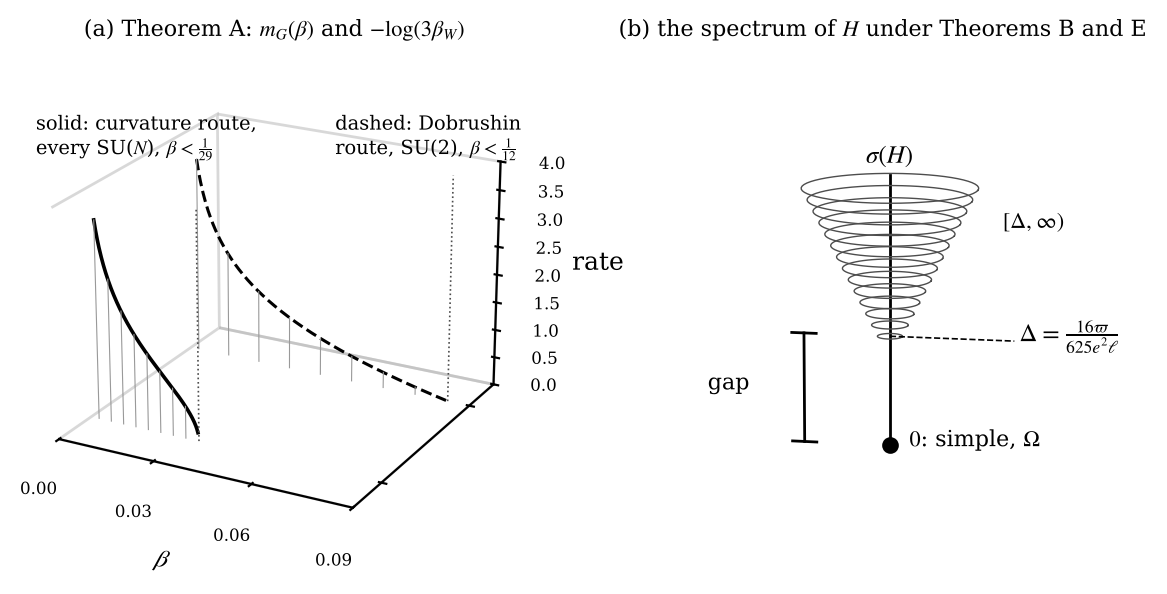
\includegraphics[width=\textwidth]{figures/fig_spectrum.png}
\caption{(a) The rates of Theorem~\ref{thm:A}: the curvature route gives $m_G(\beta)=\operatorname{arccosh}\bigl(1+\frac1{12}(\frac{\kappa_G}{N|\beta|}-\frac{29}2)\bigr)$ for $N|\beta|<\frac2{29}\kappa_G$, which for every $\SU(N)$, where $\kappa_G=N/2$, is the one curve drawn for $\beta<\frac1{29}$; the Dobrushin route for $\SU(2)$ gives $-\log(3\beta_W)=-\log(12\beta)$ for $\beta<\frac1{12}$. (b) The spectrum of the Hamiltonian under Theorems~\ref{thm:B} and~\ref{thm:E}: $0$ is a simple eigenvalue with eigenvector $\Omega$, and the rest of the spectrum lies in $[\Delta,\infty)$ with $\Delta=16\varpi/(625e^2\ell)$.}
\label{fig:spectrum}
\end{figure}

\subsection{The theories constructed on tori}

Theorem~\ref{thm:B} takes the lattice theory to infinite volume before the
lattice spacing is sent to zero. A continuum theory may also be
built in the opposite order: at a fixed physical side $L_p$ of a symmetric
torus the mesh $a_N=1/N$ is sent to zero, with couplings $\beta_{N,p}$, and the
side is sent to infinity afterwards. Section~\ref{sec:bridge} considers any
such construction whose outcome is a mixture, over a compact space $X$ of
phases carrying a measure $\nu$ of full support, of theories $S^\chi$ each
satisfying the Wightman axioms with a unique vacuum; this is hypothesis (W),
stated in full in Definition~\ref{def:WUD}; it is the shape of the
conclusion claimed by the unrefereed Lean~4 construction~\cite{OAI26,YMG26},
on which nothing below depends. At finite side the lattice state
is a thermal state at temperature $1/L_p$, and a decay estimate for its
two-point functions is not what a gap controls, so a gap for such a theory
needs more than (D). Call (U) the hypothesis that the same limit is obtained when the Euclidean time
extent of the torus is sent to infinity first, at each mesh, and
(D$_\ell$) the cube condition $\BP(n_N,\varpi)$ with $n_Na_N\le\ell$ on all
cylinders $(\Z/NL_p\Z)^3\times(\Z/M\Z)$, $M\ge2n_N+4$, at the couplings
$\beta_{N,p}$ of the construction.

\begin{mainthmE}
Under \textup{(W)}, \textup{(U)} and \textup{(D$_\ell$)} the phases $S^\chi$
all coincide, and the Wightman theory of the construction has Hamiltonian
$H$ with $\sigma(H)\subset\{0\}\cup[\Delta,\infty)$, $\Delta=16\varpi/(625e^2
\ell)$, and $0$ a simple eigenvalue.
\end{mainthmE}

This is Theorem~\ref{thm:E}; it is a theorem about the three hypotheses, and
it rests on nothing outside this paper. Two of the hypotheses can be
weakened: (U) may be replaced by the single renormalisation-free statement
(Z) that the partition function of the symmetric torus, divided by the
$NL_p$-th power of the leading eigenvalue of the transfer matrix of the
cylinder of the same side, tends to $1$ (Corollary~\ref{cor:Z}, through a
sharp inequality bounding the thermal correction of any slab observable by
that quantity, Lemma~\ref{lem:thermaldiscrepancy}); and (D$_\ell$) follows
from the slab decorrelation of Theorem~\ref{thm:D} at one physical
separation, since that theorem holds on cylinders
(Corollary~\ref{cor:cylinders}, Proposition~\ref{prop:bridgeM}). Its proof builds the transfer matrix of a
cylinder as a positive integral operator with a strictly positive kernel on
the gauge-invariant slice functions, deduces from the cube condition a gap of
the cylinder's zero-temperature Hamiltonian, carries the decay of the
renormalised two-point functions through the two limits with a constant that
depends only on the test functions, and identifies the limit of the Euclidean
vectors of the lattice theories with the vectors of the Wightman theory; the
triviality of the phase decomposition is a consequence of the same decay.
What Theorem~\ref{thm:E} does not do is prove (D$_\ell$): along the tuning of
the construction the coupling tends to infinity, and the cube condition at
weak coupling is exactly statement (D) of Sec.~\ref{sec:remains}.

\subsection{One bound at one scale}

The hypotheses of Theorem~E can be replaced by a single one that mentions
neither cubes, nor slabs, nor a gap. For a spatial torus $s$ with sides
$s_1,s_2,s_3$ and volume $V(s)$ let $\mathcal Z_s(T)$ be the partition
function of the torus $s\times(\Z/T\Z)$ divided by the $T$-th power of the
leading eigenvalue of the transfer matrix of $s$; it is the trace of the
$T$-th power of the normalised transfer matrix, and $\log\mathcal Z_s(T)$ is
the thermal part of the free energy at inverse temperature $T$. Hypothesis
(B$^{*}$) asks that, at one time extent $T_0$ of a fixed physical size,
\[
\log\mathcal Z_s(T_0)\le\gamma V(s),\qquad 2\gamma(96T_0)^3\le\tfrac1{20},
\]
for the spatial tori whose sides lie between $2T_0$ and $48T_0$.

\begin{mainthmF}
Under \textup{(W)} and \textup{(B$^{*}$)} at one physical time extent $t_0$,
the phases $S^\chi$ coincide and the Wightman theory of the construction has
$\sigma(H)\subset\{0\}\cup[\Delta,\infty)$ with $0$ a simple eigenvalue and
$\Delta\ge0.172/t_0$.
\end{mainthmF}

The full statement is in Section~\ref{ssec:onehyp}. Its proof doubles the
time extent: positivity of the transfer matrix and the exchange of the four
directions of the torus turn the bound at $T_0$ into a smaller bound at
$2T_0$ on a wider family of tori, and the iteration, which decreases doubly
exponentially, produces the gap of every large torus together with~(Z)
(Figure~\ref{fig:ascent}). The hypothesis is equivalent, up to a factor two in $\gamma$, to a finite
inequality between two partition functions,
$Z(s,T_0)^2\le e^{\gamma V(s)}Z(s,2T_0)$, in which no eigenvalue appears
(Proposition~\ref{prop:Bfinite}). It is not proved here at weak coupling,
and it cannot be easy: it contains the lattice mass gap at the scale $T_0$
(Proposition~\ref{prop:Bhard}), and for $\SU(2)$ the gap of a torus of fixed
lattice size closes as the coupling grows (Theorem~\ref{thm:gapcloses}), so
that $T_0$ must grow along the tuning (Corollary~\ref{cor:basescale}).
Appendix~\ref{app:degenerate} shows that the shortcuts which avoid the
renormalised theory, among them the limit of the parallel transporters
themselves, lead to trivial theories (Theorem~\ref{thm:haarlimit},
Proposition~\ref{prop:planar}).

\subsection{Where the cube condition holds}

\begin{mainthm}\label{thm:C}
\begin{enumerate}[label=\textup{(\roman*)},leftmargin=*]
\item At $\beta=0$, $\BP(n,1)$ holds for every $n$. For
$21N|\beta|<\kappa_G$ and $n$ large, $\BP(n,1-\alpha_n)$ holds with
$\alpha_n=N|\beta|(18n-3)/((\kappa_G-21N|\beta|)n^2)\to0$; for $\SU(2)$ the
range is $|\beta_W|<\frac5{18}$, and for $\SU(3)$ it contains
$0\le\beta_W\le0.45$.
\item For the free scalar field of lattice mass $\mu$ in $d$ dimensions the
best constant is
$\varpi=\frac{\mu^2}{n^d}\ip{\mathbf 1}{(-\Delta_D+\mu^2)^{-1}\mathbf 1}$, with
$-\Delta_D$ the Dirichlet Laplacian of the cube, and with $s=n\mu$ (the mass
times the physical size of the cube)
\[
\Bigl(\frac56\Bigr)^d\frac{s^2}{s^2+10d}\le\varpi\le\frac{s^2}{s^2+16d/9}.
\]
\item For $G=\SU(2)$ and $|\beta_W|\le\frac7{20}$, $\BP(n,\varpi)$ holds for
every $n\ge2$ with $\varpi=\frac{106}{1933}\cdot517^{-4}$, independent of $n$
and of the torus, and $\BP(n,1-259/n)$ holds for $n\ge260$. For
$0\le\beta_W\le\frac9{25}$ every torus limit is reflection positive and its
transfer matrix has spectral gap at least $7/(625\cdot2957\,e^2)$.
\end{enumerate}
\end{mainthm}

Part (ii) is the model case of the continuum tuning: the constant is uniform
in the lattice spacing at fixed $m\ell$, and it vanishes as $m\to0$. The cube
condition is therefore a quantitative statement of mass generation at the
scale $\ell$. Part (i) is proved in Sec.~\ref{sec:bpstrong} by the gauge of
Theorem~\ref{thm:A} and a weighted Dobrushin criterion for blocks of links.
No argument built on single-link updates in this gauge passes
$\beta_W=\frac13$ for $\SU(2)$ (Proposition~\ref{prop:methodlimit}). Part
(iii) passes that value by resampling \emph{stars}, the eight links at a
vertex of one parity (Sec.~\ref{sec:stars}): the perturbation of one
plaquette at a vertex enters the law of a star only through the relative
variable of two of its links, and no plaquette is internal to a star.

\subsection{Mass generation at one scale}

Statement (D) below asks for the cube condition along the continuum tuning.
Section~\ref{sec:massgen} reduces it to a hypothesis of a different kind,
closer to physics. Split a box of the lattice, all of whose widths lie
between $2d-1$ and $md-1$, into two outer parts of width $d$ and a middle of
width $d-1$ in one coordinate, fix an arbitrary configuration outside the
box, and let $\rho$ be the maximal correlation between the gauge-invariant
observables of the two outer parts under the conditional law. The hypothesis
$(\mathrm M_{d,m}(c))$ asks that $\rho\le c$ for all such boxes, splittings
and boundary conditions. Along the tuning $d\approx\ell/(2a)$, so this is a
decay of correlations across a slab of physical width about $\ell/2$,
uniform in the boundary condition.

Theorem~\ref{thm:D} proves that $(\mathrm M_{d,m}(c))$ with $c<\frac12$ and $m$
large in terms of $c$ gives $\BP(2d-1,(1-2c)^4/32)$, hence, along the tuning,
statement (D) and the continuum gap $(1-2c)^4/(1250\,e^2\ell)$ in every
nontrivial limit. The proof passes through a gap for the dynamics that
resamples overlapping patches of a box, obtained from the decorrelation of
the slabs by a Markov factorisation, and a finite-size criterion for
gauge-invariant functions in the spirit of those of Knabe~\cite{Kna88} and of
Gosset and Mozgunov~\cite{GM16} for quantum spin systems. The hypothesis also
gives exponential decay of gauge-invariant correlations under every boundary
condition, at rate $\log(1/c)/d$ per lattice spacing
(Proposition~\ref{prop:alldecay}). It holds at strong coupling at fixed $d$ and
$m$, and in two dimensions along the weak-coupling tuning
(Theorem~\ref{thm:twod}). In four dimensions it is not proved.

\subsection{The limits of the methods}

Appendix~\ref{app:obstructions} proves that several natural routes to (D)
cannot work, and locates the threshold of Theorem~\ref{thm:D}.
\begin{enumerate}[label=\textup{(\alph*)},leftmargin=*]
\item \emph{The threshold $\frac12$ is sharp.} For a massless Gaussian chain
the maximal correlation of the slab mechanism equals $\frac12$ exactly, and
the gap of the corresponding block dynamics on $M$ blocks is at most
$16/(3M)$; so no decorrelation constant $c\ge\frac12$ can give a gap uniform in
the size (Proposition~\ref{prop:gausschain}).
\item \emph{Two dimensions.} For $\SU(2)$ in two dimensions the middle slab of
a box integrates out, after an axial gauge, to a convolution power of the
heat kernel, and $(\mathrm M_{d,m}(c))$ holds with
$c=20\,e^{-3g^2(da)^2/4}$, which tends to zero as the physical size of the box
grows (Theorem~\ref{thm:twod}). The same condition for strips one link wide
fails along the tuning: a pinned strip is a Brownian bridge on $\SU(2)$, and
the antipodal boundary condition breaks a global symmetry, with correlation
close to one (Proposition~\ref{prop:strip}).
\item \emph{Curvature.} The Bakry--\'Emery constant of the Wilson measure
without gauge fixing is at most $N/2-16N|\beta|$ (Theorem~\ref{thm:fullspace});
in the gauge of
Theorem~\ref{thm:A} the constant $\frac{29}2$ cannot be replaced by anything
below $\frac{38}3$, and no Bakry--\'Emery argument for the gauge-fixed measure
reaches $|\beta_W|=\frac3{19}$ (Theorem~\ref{thm:slice}). Every smooth
plaquette action, such as an effective action at a coarse scale, obeys a bound
of the same kind (Proposition~\ref{prop:coarse}).
\item \emph{Entropy, covariances and fixed blocks.} Block entropy
factorisation implies the cube condition and so cannot be easier
(Proposition~\ref{prop:entbp}); the link covariances of every gauge-invariant
measure are $\frac14I$ and carry no information on the coupling
(Proposition~\ref{prop:linkcov}); and a single-link spectral gap, or any gap
for blocks of fixed lattice size, with constant $C_k$ satisfying $C_ka_k\to0$,
forces every continuum limit to be trivial
(Proposition~\ref{prop:fixedblocks}).
\item \emph{A gap in the limit is not enough.} If the lattice gaps $m_k$ tend
to zero, a choice of lattice spacings proportional to $m_k$ produces a
nontrivial continuum limit with a mass gap; this limit is kinematic and is not
identified with Yang--Mills theory (Theorem~\ref{thm:gaptuning}). The content
of (D) and (E) is that the gap and the nontriviality hold along the tuning of
asymptotic freedom.
\end{enumerate}

\subsection{What remains}\label{sec:remains}
\enlargethispage{3pt}

Theorems~\ref{thm:A} and~\ref{thm:C}(i), (iii) are strong-coupling theorems.
The Clay problem\footnote{The problem, as formulated by Jaffe and
Witten~\cite{JW06}, asks for a proof that for every compact simple gauge
group $G$ a nontrivial quantum Yang--Mills theory exists on $\R^4$,
satisfying axioms at least as strong as the Wightman axioms, and that it
has a mass gap: the Hamiltonian $H$ of the theory satisfies $\sigma(H)
\subset\{0\}\cup[\Delta,\infty)$ for some $\Delta>0$, with $0$ the simple
eigenvalue of the vacuum. Theorem~\ref{thm:B} and Theorem~\ref{thm:E} give
the second half of this statement, with an explicit $\Delta$, from the
hypotheses named there; the first half, existence, is hypothesis (E), or
(W).} needs the opposite end of the coupling range: the continuum
limit lives at $\beta\to\infty$, which the ranges of these theorems do not
reach. Two
statements would complete the proof of a continuum mass gap, and neither is
proved here:
\begin{enumerate}[label=\textup{(\Alph*)},leftmargin=*]
\setcounter{enumi}{3}
\item $\BP(n_k,\varpi)$ with $n_ka_k\le\ell$ along the asymptotic-freedom
tuning $\beta_k\to\infty$, uniformly in $k$;
\item convergence of the renormalised Schwinger functions to a nontrivial
limit satisfying the Osterwalder--Schrader axioms.
\end{enumerate}
Given (D) and (E), Theorem~\ref{thm:B} gives the mass gap $\Delta\ge
16\varpi/(625e^2\ell)$, and by Theorem~\ref{thm:D} statement (D) follows from
$(\mathrm M_{d_k,m}(c))$ along the tuning with $c<\frac12$. Section~\ref{sec:weak} explains why (D) is the heart of
the matter: by Theorem~\ref{thm:C}(ii) it cannot hold without a dynamically
generated mass, it fails at fixed cube size at weak coupling, and it fails in
the Coulomb phase of the abelian theory, so its proof has to use the
non-abelian structure of $G$ at every scale up to $\ell$. For the theories
built on tori, the statement of the Clay problem reduces, by
Theorem~\ref{thm:E} with the construction of~\cite{OAI26} taken as the
existence input, to (Z) or (U) together with (D$_\ell$), or with the slab
decorrelation $(\mathrm M_{d_N,m}(c))$, $c<\frac12$, at the couplings of the
construction; these remain open, and so does the mass gap. What each of
them asks is located precisely: the slab decorrelation is the maximal
correlation of two layers of a box, a quantity which in the vacuum of a
cylinder equals $e^{-m_{\mathrm{lat}}s}$ exactly, so that only its
uniformity in the boundary condition is missing
(Section~\ref{ssec:layers}), a uniformity that holds at strong coupling in
every box (Proposition~\ref{prop:layersstrong}), can fail at no fixed
box (Proposition~\ref{prop:nolock}), only along the tuning, and is
equivalent, up to constants and a change of scale, to a block Poincar\'e
inequality uniform in the boundary condition
(Section~\ref{ssec:blockgap}); and (Z) is invisible to the correlation
functions, the gap and the positivity that (W) provides, and follows
neither from (U) nor from the slab decorrelation nor from the cube
condition, even taken together (Proposition~\ref{prop:invisible},
Proposition~\ref{prop:ringsM} and Proposition~\ref{prop:ringsBP}), while
it does follow from a bound on the number of states of the cylinder per
unit of physical energy (Proposition~\ref{prop:entropyZ}), holds at
strong coupling (Proposition~\ref{prop:Zstrong}) and holds in two
dimensions along the tuning, where that number is computed exactly
(Proposition~\ref{prop:Ztwod}); no bound of the strong-coupling shape can
reach a tuning with a particle (Proposition~\ref{prop:nofixedrate}), and
(Z) is equivalent in strength to two conditions, the entropy bound at one
physical scale and the vanishing, faster than the inverse side, of the
Casimir defect of the vacuum energy under halving the spatial torus
(Proposition~\ref{prop:Zonescale}, Lemma~\ref{lem:tubes}), so that a proof of
it in four dimensions at weak coupling must count the states below the
cutoff per unit of physical volume at one scale and the low-lying states of
long tubes per unit of length; positivity in the four directions writes
both conditions, and (Z) itself, as doubling defects of the free energies of
finite tori, differences at an absolute precision $O(1)$ in which the
extensive part cancels (Proposition~\ref{prop:Zdoubling}), the gap and the
free energy per site do not control them (Proposition~\ref{prop:ringsfour}),
and the Casimir condition follows from a finite-size bound on the vacuum
energies with an exponential decay in the physical sides, the form a massive
expansion at that scale would take (Proposition~\ref{prop:FSC}). Once
the spectral gap is available on the tori of the halving chain, the
smallness of the Casimir coefficients is not needed at all: (Z) follows
from the data at one scale and a physical Casimir energy below the gap
(Theorem~\ref{thm:gapcasimir}), the Casimir coefficient is itself bounded
by the thermal corrections at aspect ratio one half (Lemma~\ref{lem:dual}),
and what remains of (C) is the exclusion, at every scale, of a branch in
which those corrections grow linearly with the scale
(Proposition~\ref{prop:dichotomy}, Theorem~\ref{thm:Crate}). Positivity alone
makes the thermal corrections at a fixed time extensive once the torus is
cut into pieces much longer than the time, and the gap carries their density
from one time to the double; so when the pressure bound at one scale is
taken on boxes elongated up to twenty-four times with respect to the time,
the gap excludes that branch and gives (Z), (K) and (C) with a rate, with no
hypothesis at a second scale (Theorem~\ref{thm:ascentZ},
Corollary~\ref{cor:branch}), and whether the bound on near-cubic boxes
suffices is a question at one scale that remains open. The free field
calibrates the condition exactly: the physical side times the Casimir defect
converges to an explicit function $c(\mu s)$ of the mass times the scale,
with $c(0)=12.56$, so that a massless field, and the free gluons of the
weak-coupling limit with the multiplicity $2\dim G$, violate (C) at every
scale, while a field of mass $\mu$ satisfies it exactly beyond the scale
$17.7/\mu$ (Theorem~\ref{thm:freelimit}, Corollary~\ref{cor:freeC},
Proposition~\ref{prop:freegluons}); the Casimir condition is a statement about
tori of about eighteen correlation lengths. The slab
hypothesis, for its part, is uniform in the boundary condition by nature:
an exact spin model with a gapped positive transfer matrix and a small
vacuum slab correlation violates it under one boundary condition
(Proposition~\ref{prop:fieldrings}), so the spectrum of the transfer
matrix alone cannot feed Theorem~\ref{thm:D}. The slab correlation is
continuous in the boundary condition, so the hypothesis is an almost sure
bound on a conditional correlation under the torus measure
(Lemma~\ref{lem:rhocont}); in the model it fails at every scale when the
field is strong, and the cube condition itself excludes the bad boundary
state there by a tunnelling function (Proposition~\ref{prop:fieldringsall});
and the patch inequality behind the finite-size criterion is equivalent,
boundary condition by boundary condition, to the local Knabe inequality on
the torus (Proposition~\ref{prop:fibre}).

\begin{figure}[t]
\centering
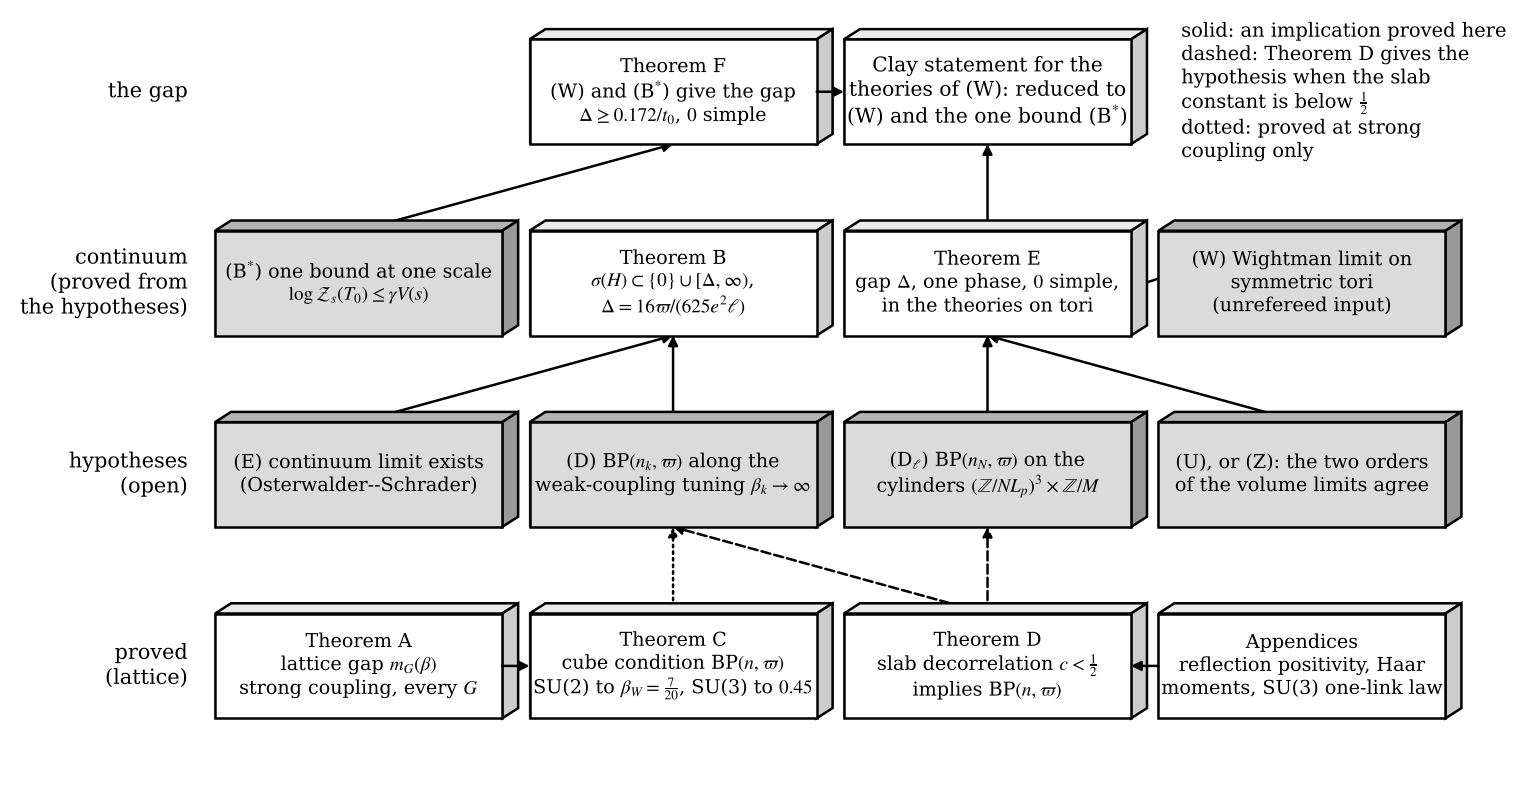
\includegraphics[width=\textwidth]{figures/fig_roadmap.png}
\caption{The logical structure of the paper. White boxes are theorems proved here, grey boxes are hypotheses; solid arrows are implications proved here, the dashed arrows are Theorem~\ref{thm:D}, which yields the cube condition when the slab decorrelation constant is below $\frac12$ (on cylinders by Corollary~\ref{cor:cylinders}), and the dotted arrow records that Theorem~\ref{thm:C} proves the cube condition at strong coupling only. With the construction of~\cite{OAI26} as the existence input (W), the statement of the Clay problem for its theories reduces to (Z) or (U), and to (D$_\ell$) or the slab decorrelation (Theorem~E), and all of these follow from the single bound (B$^{*}$) at one scale (Theorem~F).}
\label{fig:roadmap}
\end{figure}

\subsection{Related work}

Strong-coupling clustering goes back to Osterwalder and Seiler \cite{OSei78}
and Seiler \cite{Sei82}; probabilistic treatments include the survey of
Chatterjee \cite{Chat19}, the Langevin approach of Shen, Zhu and Zhu
\cite{SZZ23}, whose Bakry--\'Emery argument we sharpen, and correlation
decay for finite gauge groups at weak coupling by Adhikari and Cao \cite{AC25}.
In two dimensions the continuum measure is known
\cite{GKS89,Dri89,Lev03}. The transfer matrix of lattice gauge theory is
L\"uscher's \cite{Lus77}, with the temporal gauge and the positivity of the
transfer matrix in Creutz's form~\cite{Cre77}, and the Osterwalder--Schrader reconstruction on the
lattice is due to Osterwalder and Seiler \cite{OSei78}. 
One of us (I.~J.~S.) has formalised in Lean~4 with Mathlib, in a separate
development, without
unproved statements and with only the standard axioms, several ingredients of
the strong-coupling analysis on periodic lattices: the Haar probability on
$\SU(N)$, an infinite-volume Gibbs state obtained as a limit of torus states,
site reflection positivity and the transfer matrix, the Holley--Stroock~\cite{HS87}
comparison, Dobrushin's covariance bounds, and the passage from decay of
correlations to a transfer-matrix gap (one direction of
Proposition~\ref{prop:gapdecay}). For the periodic state it proves a
transfer-matrix gap for every $N$ at $\beta_W<5.9\cdot10^{-5}$, and explicit
single-link heat-bath gaps on boxes of side fifteen for $\SU(2)$ at
$\beta_W\le0.166$ and for $\SU(3)$ at $\beta_W\le0.38$ (the coupling there is
$\beta_W/2$). It also proves, by a Poincar\'e inequality and a light-cone
argument different from Lemma~\ref{lem:speed}, that an ungauged one-cube
influence condition gives a lattice gap of order $1/n$; this is a variant of
the lattice step, Theorem~\ref{thm:decay} and Corollary~\ref{cor:latticegap},
at a smaller rate. The continuum step, the gauge
fixing and the curvature bounds are not part of that development, which shares
with this paper the open hypothesis (D).


\section{Lattice gauge theory and the transfer matrix}\label{sec:lattice}

Write $e_0,\dots,e_3$ for the unit vectors of $\Z^4$, $(x,\mu)$ for the link
from $x$ to $x+e_\mu$, and $Q_{(x,\mu)}^{-1}$ for the variable of the reversed
link. A box $\Lambda$ is a product of four finite intervals, with its set
$E(\Lambda)$ of links and its set $P(\Lambda)$ of plaquettes. For a plaquette
at $x$ in the plane $\mu<\nu$ with links $e_1=(x,\mu)$, $e_2=(x+e_\mu,\nu)$,
$e_3=(x+e_\nu,\mu)$, $e_4=(x,\nu)$, put $Q_p=Q_{e_1}Q_{e_2}Q_{e_3}^*Q_{e_4}^*$.
With $dQ$ the Haar probability measure of $G$, the Wilson measure of a box
with free boundary is
\[
W_\Lambda(dQ)=\frac1{Z_\Lambda}\exp\Bigl(N\beta\sum_{p\in P(\Lambda)}\ReTr
Q_p\Bigr)\prod_{e\in E(\Lambda)}dQ_e ,
\]
and the Wilson measure $\mu_L$ of the torus $\Lambda_L=(\Z/L\Z)^4$ is defined
in the same way with all links and plaquettes of $\Lambda_L$. Both are
invariant under the gauge transformations $Q_{(x,y)}\mapsto g_xQ_{(x,y)}
g_y^{-1}$. A function of finitely many links is a local observable, and it
is gauge invariant if it is invariant under these transformations. For
$\beta\ge0$ the measures are reflection positive for reflections in lattice
hyperplanes through sites and in hyperplanes bisecting links, on boxes
symmetric under the reflection and on tori of even side~\cite{OSei78}.

Let $\omega$ be a state on the gauge-invariant local observables of $\Z^4$
that is invariant under translations and reflection positive in this sense.
The Osterwalder--Schrader construction~\cite{OS73,OS75,OSei78} gives a
Hilbert space $\mathcal H$ with a unit vector $\Omega$, a map $F\mapsto\Psi_F$
from the observables at nonnegative times to $\mathcal H$ with dense range,
and a self-adjoint transfer matrix $0\le\mathbb T\le1$ with $\mathbb T\Omega=
\Omega$ and
\[
\ip{\Psi_F}{\mathbb T^t\Psi_H}=\omega\bigl(\vartheta(\bar F)\,\tau_tH\bigr),
\qquad t\in\Z_{\ge0},
\]
where $\vartheta$ is the time reflection and $\tau_t$ the time translation;
$\Psi_F$ is the class of $F$ for the positive semidefinite form
$\omega(\vartheta(\bar F)H)$, and $\|\Psi_F\|^2\le\omega(|F|^2)$. The
\emph{spectral gap} of $\mathbb T$ is $m$ if its spectrum on $\Omega^\perp$
lies in $[0,e^{-m}]$.

\begin{proposition}\label{prop:gapdecay}
Let $m>0$ and let $\mathcal F$ be a class of gauge-invariant local
observables, supported at nonnegative times, that is dense in $L^2(\omega)$
on each bounded time support. If for every $F\in\mathcal F$ there is
$C_F<\infty$ with
\[
\omega(\vartheta(\bar F)\tau_tF)-|\omega(F)|^2\le C_Fe^{-mt}\qquad(t\ge0),
\]
then $\mathbb T$ has spectral gap at least $m$.
\end{proposition}

\begin{proof}
Put $\Psi'_F=\Psi_F-\ip\Omega{\Psi_F}\Omega$, so that the left side equals
$\ip{\Psi'_F}{\mathbb T^t\Psi'_F}=\int\lambda^t\,d\sigma_F(\lambda)$, with
$\sigma_F$ the spectral measure of $\mathbb T$ at $\Psi'_F$. For $\delta>0$
this is at least $\sigma_F((e^{-m+\delta},1])e^{(-m+\delta)t}$, which exceeds
$C_Fe^{-mt}$ for large $t$ unless $\sigma_F((e^{-m+\delta},1])=0$. So the
spectral projection of $(e^{-m},1]$ annihilates every $\Psi'_F$. These vectors
are dense in $\Omega^\perp$, because $\|\Psi_F\|^2\le\omega(|F|^2)$ and the
class is dense, so the projection vanishes on $\Omega^\perp$.
\end{proof}

The decay of a single two-point function does not suffice: it places only
one spectral measure in $[0,e^{-m}]$, and the density of the class is what
gives the gap.


\section{The line field}\label{sec:linefield}

A \emph{direction field} is a map $\sigma:\Z^4\to\{0,1,2,3\}$; its links
are $F=\{(x,\sigma(x)):x\in\Z^4\}$. At each site put $\pi_x(\mu)=
\sigma(x+e_\mu)$. The plaquette at $x$ in the plane $\{\mu,\nu\}$ contains
\begin{equation}\label{eq:count}
[\sigma(x)\in\{\mu,\nu\}]+[\pi_x(\mu)=\nu]+[\pi_x(\nu)=\mu]
\end{equation}
links of $F$.

\begin{lemma}\label{lem:cycle}
Every plaquette contains exactly one link of $F$ if and only if, at every
site $x$, $\pi_x$ fixes $\sigma(x)$ and permutes the other three directions
cyclically.
\end{lemma}

\begin{proof}
Fix $x$, let $s=\sigma(x)$ and let $R$ be the other three directions. For the
plane $\{s,\nu\}$ the count~\eqref{eq:count} is $1+[\pi_x(s)=\nu]+[\pi_x(\nu)
=s]$, which equals one for all $\nu\in R$ exactly when $\pi_x$ fixes $s$ and
maps $R$ into $R$. For a plane $\{\mu,\nu\}\subset R$ the count is
$[\pi_x(\mu)=\nu]+[\pi_x(\nu)=\mu]$. Draw an arrow $\mu\to\pi_x(\mu)$ whenever
$\pi_x(\mu)\in R\setminus\{\mu\}$; each vertex has at most one outgoing arrow,
and the condition asks for exactly one arrow on each of the three pairs. Three
arrows on three vertices with out-degree at most one give out-degree one
everywhere, and such a tournament is a directed three-cycle.
\end{proof}

From now on $\sigma$ is the field of period two of Table~\ref{tab:sigma} in
Appendix~\ref{app:table}; in each row $\pi_x$ fixes $\sigma(x)$ and is a
three-cycle on the other directions, so every plaquette contains exactly one
link of $F$.\footnote{A field with one link of $F$ at every site and one in
every plaquette can exist only in four dimensions: a site carries
$d(d-1)/2$ plaquettes at which it is the base point and a link lies in
$2(d-1)$ plaquettes, and the two counts agree only for $d=4$.} Call the links
outside $F$ \emph{active} and write $A$ for their set.

\begin{figure}[t]
\centering
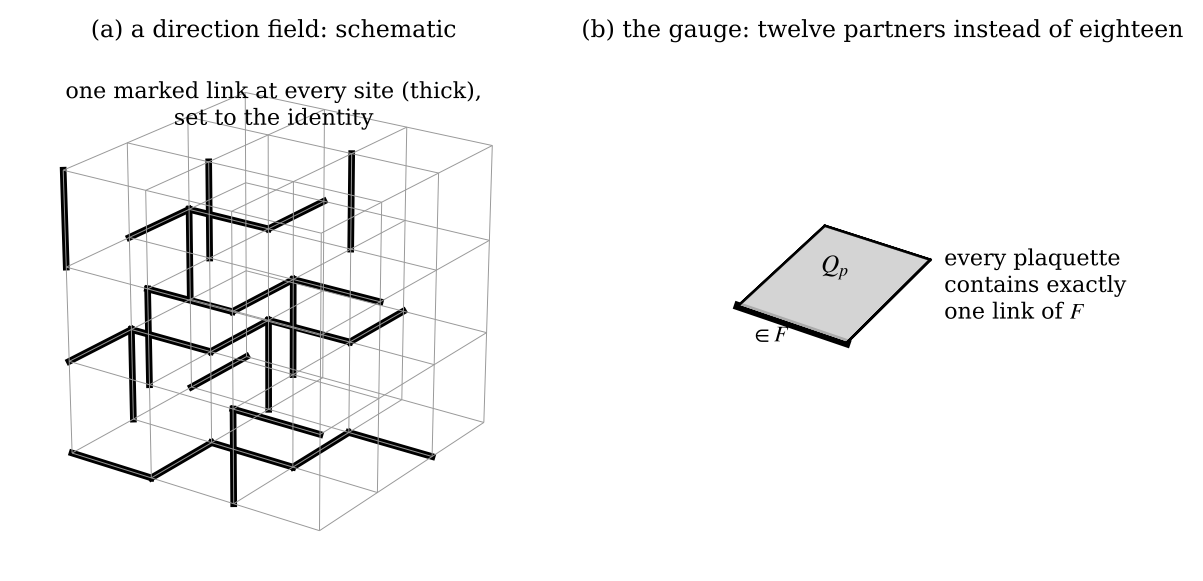
\includegraphics[width=\textwidth]{figures/fig_linefield.png}
\caption{(a) A direction field on a three-dimensional slice, drawn schematically: one marked link at every site (thick), set to the identity by a gauge transformation; the marked links form lines. (b) In this gauge every plaquette contains exactly one link of $F$, so an active link shares a plaquette with twelve other active links instead of eighteen (Lemma~\ref{lem:structure}); the actual field is four-dimensional and is listed in Appendix~\ref{app:table}.}
\label{fig:linefield}
\end{figure}

\begin{lemma}\label{lem:structure}\leavevmode
\begin{enumerate}[label=\textup{(\roman*)},leftmargin=*]
\item $F$ is a disjoint union of bi-infinite straight lines, one through every
site; hence $F\cap E(\Lambda)$ is a forest for every box $\Lambda$.
\item An active link $e=(x,\mu)$ lies in six plaquettes. In four of them the
link of $F$ shares an end point with $e$; in the other two it is opposite to
$e$.
\item Every active link shares a plaquette with exactly twelve other active
links, two in each of its plaquettes, and two links share at most one
plaquette.
\end{enumerate}
\end{lemma}

\begin{proof}
(i) Since $\pi_x$ fixes $\sigma(x)$, $\sigma(x+e_{\sigma(x)})=\sigma(x)$, and since
$\sigma$ has period two, also $\sigma(x-e_{\sigma(x)})=\sigma(x)$. If $(x-e_\nu,\nu)
\in F$, straightness at $x-e_\nu$ gives $\sigma(x)=\nu$, so the incoming link of
$F$ at $x$ is unique and continues the outgoing one. A line meets a box in a
segment.

(ii) A link of $F$ sharing an end point with $e$ is the outgoing or incoming
link of $F$ at $x$, of direction $s=\sigma(x)\ne\mu$, or at $x+e_\mu$, of
direction $t=\pi_x(\mu)\in R\setminus\{\mu\}$. They lie in the two plaquettes of
$e$ in the plane $\{\mu,s\}$ and the two in the plane $\{\mu,t\}$, four distinct
plaquettes as $s\ne t$. In the two plaquettes of the remaining plane
$\{\mu,\rho\}$ the unique link of $F$ touches neither end of $e$, so it is the
opposite link.

(iii) Each plaquette of $e$ contains $e$, one link of $F$ and two other links.
\end{proof}


\section{Gauge fixing and the free-boundary state}\label{sec:state}

For a function $O$ of the links let $O^F$ be $O$ with every link of $F$ set to
the identity.

\begin{lemma}[gauge fixing]\label{lem:gaugefix}
Let $\mu^F_\Lambda$ be the probability measure on $G^{A\cap E(\Lambda)}$ with
density proportional to $\exp(N\beta\sum_{p\in P(\Lambda)}\ReTr Q^F_p)$. For
every gauge-invariant $O$ on $G^{E(\Lambda)}$, $W_\Lambda(O)=\mu^F_\Lambda(O^F)$.
\end{lemma}

\begin{proof}
Each segment of $F\cap E(\Lambda)$ is a path $x_0,\dots,x_k$. Given the
variables on $F$, put $g_{x_0}=1$ and $g_{x_{i+1}}=g_{x_i}Q_{(x_i,x_{i+1})}$
along every segment. The transformed field equals the identity on $F\cap
E(\Lambda)$, and for fixed values on $F$ the map from the active variables to
the transformed ones is a product of translations, which preserve Haar
measure. Gauge invariance of the action and of $O$ gives the claim.
\end{proof}

No holonomy remains because $F\cap E(\Lambda)$ is a forest. The measures
$\mu^F_\Lambda$ are finite-volume versions of the specification $\gamma^F$ on
$G^A$ in which $\gamma^F_e$ resamples an active $Q_e$ from the law with density
proportional to $\exp(N\beta\sum_{p\ni e}\ReTr Q^F_p)$ given the other active
links. Fix a bi-invariant metric $\delta$ on $G$ of diameter $D$ and define the
Kantorovich coefficients
\[
C_{ee'}=\sup\frac{W_1\bigl(\gamma^F_e(\cdot\mid Q),\gamma^F_e(\cdot\mid Q')\bigr)}
{\delta(Q_{e'},Q'_{e'})},
\]
the supremum over configurations that differ only at $e'$; $W_1$ is the
Kantorovich distance~\cite{Vil09}, and $C_{ee'}=0$ unless $e$ and $e'$ share a
plaquette.

\begin{lemma}[comparison]\label{lem:comparison}
Suppose every row and column of $(C_{ee'})$ sums to at most $\alpha<1$, and let
$\lambda>0$ with $\theta=\alpha e^\lambda<1$. Let $S\subset A$ and let $\mu_1,\mu_2$
be probability measures on $G^A$ invariant under $\gamma^F_e$ for $e\notin S$.
Let $T\subset A\setminus S$ be finite, $w_b=e^{-\lambda\dist(b,T)}$ with the
distance of link midpoints, and suppose $\sum_{z\in S}w_z<\infty$. There is a
coupling of $\mu_1$ and $\mu_2$ with $\varrho(b)=\E\,\delta(\sigma_b,\sigma'_b)$
satisfying
\[
\sum_{b\notin S}w_b\varrho(b)\le\frac{\theta D}{1-\theta}\sum_{z\in S}w_z ,
\]
and $\mu_1=\mu_2$ if $S=\emptyset$.
\end{lemma}

\begin{proof}
The couplings form a weakly compact set on which $\Psi(\pi)=\sum_bw_b\E_\pi
\delta(\sigma_b,\sigma'_b)$ is continuous; let $\pi^*$ minimise it. For $e\notin S$
replace $(\sigma_e,\sigma'_e)$ by a sample of an optimal coupling of
$\gamma^F_e(\cdot\mid\sigma)$ and $\gamma^F_e(\cdot\mid\sigma')$, chosen
measurably~\cite[Cor.~5.22]{Vil09}. Both $\mu_i$ are invariant, so this is again
a coupling, and changing the links that enter $\gamma^F_e$ one at a time gives
$\varrho(e)\le\sum_{e'}C_{ee'}\varrho(e')$ by minimality. Multiply by $w_e$ and sum
over $e\notin S$; where $C_{ee'}\ne0$, $w_e\le e^\lambda w_{e'}$, so
$\sum_{e\notin S}w_e\varrho(e)\le\theta[\sum_{e'\notin S}w_{e'}\varrho(e')+D\sum_{z
\in S}w_z]$. If $S=\emptyset$ this forces $\varrho\equiv0$.
\end{proof}

Conditioning on the links of the support of $H$~\cite[Ch.~3]{Kal21} and
applying the lemma to the two conditional measures gives, for the Gibbs
measure $\mu$ of $\gamma^F$, a local $F'$ that is $L$-Lipschitz in each link and
a bounded $H$ with finite support disjoint from that of $F'$,
\begin{equation}\label{eq:decay}
|\Cov_\mu(F',H)|\le\|H\|_\infty L\,\frac{\theta D}{1-\theta}\,|\operatorname{supp}H|\,
e^{-\lambda\dist(\operatorname{supp}F',\operatorname{supp}H)} .
\end{equation}

\begin{proposition}\label{prop:state}
Suppose every row and column of $(C_{ee'})$ sums to at most $\alpha<1$. Then
$\gamma^F$ has a unique Gibbs measure $\mu_F$; for every gauge-invariant local $O$
the limit $\omega(O)=\lim W_\Lambda(O)$ exists along every sequence of boxes
exhausting $\Z^4$ and equals $\mu_F(O^F)$; $\omega$ is invariant under
translations and the hypercubic group; truncated correlations of Lipschitz
gauge-invariant observables decay at every rate below $-\log\alpha$; and for
$\beta\ge0$, $\omega$ is reflection positive and its transfer matrix has
spectral gap at least $-\log\alpha$.
\end{proposition}

\begin{proof}
Gibbs measures exist by compactness and coincide by Lemma~\ref{lem:comparison}
with $S=\emptyset$. Extend $\mu^F_\Lambda$ by Haar measure outside $\Lambda$ and
let $S$ be the set of active links with a plaquette outside $P(\Lambda)$; off $S$
the extended measure is invariant under $\gamma^F_e$. Lemma~\ref{lem:comparison}
with $T$ the support of $O^F$ bounds $|\mu^F_\Lambda(O^F)-\mu_F(O^F)|$ by
$C_TR^3e^{-\lambda R}$, $R$ the distance from $T$ to the complement of $\Lambda$,
for Lipschitz $O$, and uniform approximation handles continuous $O$;
Lemma~\ref{lem:gaugefix} identifies $\mu^F_\Lambda(O^F)$ with $W_\Lambda(O)$. Since
$W_\Lambda(\tau_vO)=W_{\Lambda-v}(O)$ and the limit does not depend on the
exhausting sequence, $\omega$ is invariant; the line field is a device for
computing $W_\Lambda$ and is never moved. Reflection positivity of $W_\Lambda$ on
symmetric boxes passes to the limit. The decay is~\eqref{eq:decay}, since
$\Cov_\omega(O,O')=\Cov_{\mu_F}(O^F,O'^F)$. Lipschitz gauge-invariant functions
are dense in the gauge-invariant part of $L^2(\omega)$ on every support, being
Lipschitz functions on the compact quotient by the gauge group, so
Proposition~\ref{prop:gapdecay} gives the gap.
\end{proof}

\begin{proof}[Proof of Theorem~\ref{thm:A} for $\SU(2)$]
Identify $\SU(2)$ with the unit quaternions and use the chordal metric. For an
active link $e$ and a plaquette $p\ni e$ let $s_p$ be the product of the other
three variables, ordered so that $\operatorname{Re}(Q_es_p)=\frac12\Tr Q_p$, with
links of $F$ equal to one. Since $N\beta\ReTr Q_p=4\beta\ip{Q_e}{\bar s_p}$ in
$\R^4$, the conditional law of $Q_e$ is the von Mises--Fisher law $\nu_b(dx)
\propto e^{\ip xb}dx$ on $S^3$ with $b=4\beta\sum_{p\ni e}\bar s_p$. Moving a
partner $e'$ by $\delta$ moves one staple by an isometric image of that
displacement, hence $b$ by $4|\beta|\delta$, and the sharp
quarter (Theorem~\ref{q-thm:quarter} in Appendix~\ref{app:sharp}), $W_1(\nu_b,\nu_{b'})\le\frac14|b-b'|$, gives
$C_{ee'}\le|\beta|$. By Lemma~\ref{lem:structure}(iii) every row and column has
twelve nonzero entries, so $\alpha\le12|\beta|=3|\beta_W|$, and
Proposition~\ref{prop:state} applies for $|\beta_W|<\frac13$.
\end{proof}

The value $\frac13$ is the end of this argument: at $b=0$ the derivative of
$\nu_b$ has Kantorovich norm exactly $\frac14$, the six staples of an active
link can be arranged with sum zero while one of them moves freely, and so
every row sum of the matrix is exactly $3|\beta_W|$. Without the gauge every
link has eighteen partners, each entry of the matrix is again at most
$|\beta|$, and the same argument stops at $18|\beta|=1$, that is at
$\beta_W=\frac29$.


\section{Curvature in the gauge}\label{sec:curvature}

In this section $G\subset\U(N)$ is closed and connected with Lie algebra $\g$
and the inner product $\ip XY=-\Tr(XY)$. A tangent vector at a field $Q$ is
$v=(X_eQ_e)$ with $X_e\in\g$, and $|v|^2=\sum_e|X_e|^2$. For the plaquette $p$
at $x$ in the plane $\mu<\nu$, with links $e_1,\dots,e_4$ as in
Sec.~\ref{sec:lattice}, transport the vectors to $x$,
\[
Y_1=X_{e_1},\quad Y_2=Q_{e_1}X_{e_2}Q_{e_1}^*,\quad
Y_3=Q_{e_4}X_{e_3}Q_{e_4}^*,\quad Y_4=X_{e_4},
\]
and write $W=Q_p$. Along the geodesics $Q_e(t)=e^{tX_e}Q_e$ the plaquette
variable is $Q_p(t)=e^{tY_1}e^{tY_2}We^{-tY_3}e^{-tY_4}$, and differentiating
twice gives the second derivative of $\ReTr Q_p$,
\begin{equation}\label{eq:fp}
f_p=\sum_{i=1}^4\ReTr(Y_i^2W)+2\ReTr(Y_1Y_2W)+2\ReTr(Y_3Y_4W)
-2\!\!\sum_{i\in\{1,2\},\,j\in\{3,4\}}\!\!\ReTr(Y_iWY_j),
\end{equation}
so that $\Hess S_0(v,v)=\sum_pf_p$ for $S_0=\sum_p\ReTr Q_p$. The
\emph{corner form} of $p$ is
\begin{equation}\label{eq:corner}
c_p=2\ip{Y_1}{Y_4}-2\ip{Y_1}{Y_2}+2\ip{Y_2}{WY_3W^*}-2\ip{Y_3}{Y_4};
\end{equation}
it collects the inner products of the vectors of two links that meet at a
right angle at a corner of $p$.

\begin{lemma}[divergence identity]\label{lem:identity}
On $\Z^4$, or on a box with free boundary, for every field $Q$ and every
square-summable $X$,
\[
\sum_y\Bigl[|D_yX|^2+\sum_\mu\bigl|X_{y,\mu}+Q^*_{y-e_\mu,\mu}X_{y-e_\mu,\mu}
Q_{y-e_\mu,\mu}\bigr|^2\Bigr]=4|X|^2+\sum_pc_p ,
\]
where $D_yX=\sum_\mu[X_{y,\mu}-Q^*_{y-e_\mu,\mu}X_{y-e_\mu,\mu}Q_{y-e_\mu,\mu}]$
is the covariant divergence and terms with a link outside the box are
omitted.
\end{lemma}

\begin{proof}
At a site $y$ let $o_\mu$ be the vector of the outgoing link of direction $\mu$
and $i_\mu$ the transported vector of the incoming one, so that $D_yX=\sum_\mu
(o_\mu-i_\mu)$. Every link is outgoing at one end and incoming at the other, so
the squares $|o_\mu|^2+|i_\mu|^2$, which occur once in $|D_yX|^2$ and once in
$|o_\mu+i_\mu|^2$, add up to $4|X|^2$. The collinear cross term
$-2\ip{o_\mu}{i_\mu}$ of $|D_yX|^2$ cancels the term $+2\ip{o_\mu}{i_\mu}$ of
$|o_\mu+i_\mu|^2$. Every remaining cross term of $|D_yX|^2$ pairs two
perpendicular ends at $y$, and such a pair is a corner of exactly one
plaquette, with the sign and transport of~\eqref{eq:corner}; in a box two
perpendicular ends at $y$ span a plaquette of the box.
\end{proof}

\begin{lemma}[one plaquette]\label{lem:local}
Let $k\in\{1,2,3,4\}$, let $k\pm1$ \textup{(}mod $4$\textup{)} be the
positions adjacent to $k$ and $k+2$ the opposite one. For every $N$, every
$W\in\U(N)$ and all $Y_1,\dots,Y_4\in\mathfrak u(N)$ with $Y_k=0$,
\[
\pm f_p+\tfrac9{10}c_p\le\tfrac{21}{10}\bigl(|Y_{k-1}|^2+|Y_{k+1}|^2\bigr)
+\tfrac54|Y_{k+2}|^2 .
\]
\end{lemma}

\begin{proof}
Replacing $W$ by $-W$ changes the sign of $f_p$ and fixes $c_p$, so the sign
$+$ suffices, and conjugation by a unitary matrix preserves both sides, so we
may take $W=\operatorname{diag}(w_a)$. The difference $\mathcal F$ of the two
sides then splits into a block for each diagonal position $a$, in the real
variables $y_i=-i(Y_i)_{aa}$, and a block for each pair $a\ne b$, in the
complex variables $z_i=(Y_i)_{ab}$, since $(Y_i)_{ba}=-\bar z_i$.
Appendix~\ref{app:blocks} shows that every block is positive definite.
\end{proof}

\begin{theorem}[Hessian bound]\label{thm:hess}
For every closed subgroup $G\subset\U(N)$, every box or $\Z^4$, every field
$Q$ and every tangent vector $v$ that vanishes on the links of $F$,
\[
|\Hess S_0(v,v)|\le\tfrac{29}2|v|^2 .
\]
\end{theorem}

\begin{proof}
Every plaquette has exactly one link of $F$, on which $X$ vanishes, and by
Lemma~\ref{lem:structure}(ii) each active link is adjacent to that link in
four of its plaquettes and opposite to it in two. Summing
Lemma~\ref{lem:local} over the plaquettes,
\[
\sum_p\bigl(\pm f_p+\tfrac9{10}c_p\bigr)\le\bigl(4\cdot\tfrac{21}{10}+2\cdot
\tfrac54\bigr)|X|^2=\tfrac{109}{10}|X|^2 .
\]
By Lemma~\ref{lem:identity}, $\frac9{10}\sum_pc_p=\frac9{10}\Sigma-\frac{36}{10}
|X|^2$ with $\Sigma\ge0$ the left side of that lemma. Hence $\pm\Hess S_0(v,v)
\le(\frac{109}{10}+\frac{36}{10})|X|^2=\frac{29}2|X|^2$; links near the boundary
of a box lie in fewer plaquettes and receive less. Both lemmas concern
vectors in $\mathfrak u(N)$, so the bound holds on every closed subgroup, whose
geodesics $e^{tX}Q_e$ with $X\in\g$ are geodesics of $\U(N)$.
\end{proof}

The factor $\frac9{10}$ lets the divergence identity pay for the corners at
the price $\frac{36}{10}$ while the blocks of one plaquette stay positive.
Without the gauge the Hessian attains the value $16$ (Theorem~\ref{thm:fullspace}).

\begin{lemma}[Ricci curvature]\label{lem:ricci}
Let $G\subset\U(N)$ be closed and connected with simple Lie algebra, and let
$\mathfrak t\subset\g$ be a maximal abelian subalgebra. Write the eigenvalues
of $\operatorname{ad}H$ on $\g\otimes\C$ and of $H$ on $\C^N$, $H\in\mathfrak t$, as
$i\alpha(H)$ and $i\mu(H)$, over the roots $\alpha$ and the weights $\mu$ counted
with multiplicity. Then $\Ric_G=\kappa_G\ip\cdot\cdot$ with
\[
\kappa_G=\frac{\sum_\alpha\alpha(H)^2}{4\sum_\mu\mu(H)^2}=\frac{h^\vee}{2\ell_\rho}
\qquad(0\ne H\in\mathfrak t).
\]
\end{lemma}

\begin{proof}
For a bi-invariant metric $R(X,Y)Z=-\frac14[[X,Y],Z]$ on left-invariant fields
\cite[Sect.~7]{Mil76}, so for an orthonormal basis $(E_i)$,
$\Ric(X,X)=\frac14\sum_i|[X,E_i]|^2=-\frac14\Tr(\operatorname{ad}X)^2$. The
Killing form and $\ip\cdot\cdot$ are invariant and $\g$ is simple, so the
Killing form is $-4\kappa\ip\cdot\cdot$ for a constant $\kappa$, and on
$\mathfrak t$ the two forms are $-\sum_\alpha\alpha(H)^2$ and $\sum_\mu\mu(H)^2$.
For $H$ the coroot of the highest root, $\sum_\alpha\alpha(H)^2=4h^\vee$ and
$\sum_\mu\mu(H)^2=2\ell_\rho$~\cite[Ch.~6]{Kac90}.
\end{proof}

\begin{table}[t]
\caption{The curvature $\kappa_G=h^\vee/(2\ell_\rho)$ in a faithful
representation of least dimension $N$, and the range of Theorem~\ref{thm:A}
for $\beta_W=N^2\beta$.}
\label{tab:groups}
\begin{tabular}{llcccc}
\toprule
Group&$\rho$&$h^\vee$&$\ell_\rho$&$\kappa_G$&$\beta_W<$\\
\midrule
$\SU(N)$, $N\ge2$&$\C^N$&$N$&$1$&$\frac N2$&$\frac{N^2}{29}$\\
$\SO(N)$, $N\ge5$&$\R^N$&$N-2$&$2$&$\frac{N-2}4$&$\frac{N(N-2)}{58}$\\
$\mathrm{Sp}(n)$, $n\ge2$&$\C^{2n}$&$n+1$&$1$&$\frac{n+1}2$&$\frac{2n(n+1)}{29}$\\
$G_2$&$7$&$4$&$2$&$1$&$\frac{14}{29}$\\
$F_4$&$26$&$9$&$6$&$\frac34$&$\frac{39}{29}$\\
$E_6$&$27$&$12$&$6$&$1$&$\frac{54}{29}$\\
$E_7$&$56$&$18$&$12$&$\frac34$&$\frac{84}{29}$\\
$E_8$&$248$&$30$&$60$&$\frac14$&$\frac{124}{29}$\\
\bottomrule
\end{tabular}
\end{table}

For two links $e\ne e'$ of a plaquette $p$ write $\Hess\ReTr Q_p(v,v)=
\sum_{e,e'\in p}H^p_{ee'}(X_e,X_{e'})$ with $H^p_{ee'}(a,b)=H^p_{e'e}(b,a)$. By
\eqref{eq:fp} a mixed block is, after isometric transport, $\pm\ReTr(abW)$ or
$\pm\ReTr(aWb)$, so
\begin{equation}\label{eq:mixed}
|H^p_{ee'}(a,b)|\le|a|\,|b| .
\end{equation}

\subsection{Decay with an explicit rate}

Let $A'$ be a finite set of active links and $P'$ a finite set of plaquettes
whose active links lie in $A'$. Call $S=\sum_{p\in P'}c_p\ReTr Q^F_p$, $0\le
c_p\le1$, \emph{admissible} if $|\Hess S(v,v)|\le\frac{29}2|v|^2$ for $v$
tangent to $G^{A'}$. By Theorem~\ref{thm:hess} the action $S_\Lambda=\sum_{p\in
P(\Lambda)}\ReTr Q^F_p$ of a box is admissible, and so is every convex combination
of admissible actions; by~\eqref{eq:mixed} and Lemma~\ref{lem:structure}(iii)
the mixed blocks of $\Hess S$ have norm at most one and each link has at most
twelve partners. Let $\mu$ have density proportional to $e^{N\beta S}$ on
$G^{A'}$, let $L=\Delta+N\beta\ip{\nabla S}{\nabla\cdot}$ be its Langevin generator,
self-adjoint in $L^2(\mu)$, and $P_t=e^{tL}$. For weights $w>0$ on $A'$ put
$\Gamma^w(f)=\sum_ew_e|\nabla_ef|^2$, with $\nabla_e$ the gradient in the factor of
$e$; $\Gamma$ is the case $w\equiv1$.

\begin{lemma}\label{lem:weighted}
Let $G$ have semisimple Lie algebra, $\lambda\ge0$, $w_e=e^{\lambda d_e}$ with
$|d_e-d_{e'}|\le1$ for partners, and
\[
K_\lambda=\kappa_G-N|\beta|\Bigl(\tfrac{29}2+12\bigl(\cosh\tfrac\lambda2-1\bigr)\Bigr).
\]
Then $\Gamma^w(P_tf)\le e^{-2K_\lambda t}P_t\Gamma^w(f)$ for smooth $f$ and $t\ge0$.
\end{lemma}

\begin{proof}
Put $V=-N\beta S$. On the product $G^{A'}$ the projection to one factor is
parallel and the Ricci tensor is block diagonal, so Bochner's formula
applied factor by factor gives
\[
\tfrac12L\Gamma^w(g)-\Gamma^w(g,Lg)=\sum_ew_e\bigl(|\nabla\nabla_eg|^2+\Ric_G(\nabla_e
g,\nabla_eg)\bigr)+\sum_{e,e'}w_e\Hess V_{ee'}(\nabla_eg,\nabla_{e'}g).
\]
With $u_e=\nabla_eg$, $v_e=\sqrt{w_e}u_e$ and the symmetry of $\Hess V$, the last
sum is
\[
\Hess V(v,v)+\sum_{e\ne e'}\Bigl(\cosh\tfrac{\lambda(d_e-d_{e'})}2-1\Bigr)\Hess
V_{ee'}(v_e,v_{e'}),
\]
since $(w_e+w_{e'})/(2\sqrt{w_ew_{e'}})=\cosh\frac{\lambda(d_e-d_{e'})}2$. The first
term is at least $-\frac{29}2N|\beta||v|^2$; in the second only partners
contribute, each with coefficient at most $\cosh\frac\lambda2-1$ and a block of
norm at most $N|\beta|$, and with twelve partners it is at least
$-12(\cosh\frac\lambda2-1)N|\beta||v|^2$. As $\Ric_G\ge\kappa_G$ and $|v|^2=
\Gamma^w(g)$, the left side is at least $K_\lambda\Gamma^w(g)$. For
$\varphi(s)=P_s\Gamma^w(P_{t-s}f)$ this gives $\varphi'\ge2K_\lambda\varphi$, hence
$\varphi(0)\le e^{-2K_\lambda t}\varphi(t)$.
\end{proof}

\begin{lemma}\label{lem:decayrate}
Suppose $K_\lambda>0$. Let $f,g$ be smooth functions of the links of $A_f$ and
$B_g$, and let $D$ be the graph distance from $A_f$ to $B_g$ in the graph on
$A'$ whose edges join partners. Then
\[
|\Cov_\mu(f,g)|\le\frac{e^{-\lambda D/2}}{K_\lambda}\,\|\nabla f\|_\infty
\sum_{e\in B_g}\|\nabla_eg\|_\infty .
\]
\end{lemma}

\begin{proof}
Lemma~\ref{lem:weighted} with $\lambda=0$ shows that $P_tf\to\mu(f)$ uniformly,
so $\Cov_\mu(f,g)=\int_0^\infty\mu(\Gamma(P_tf,g))\,dt$. Let $d_e$ be the smaller of
$D$ and the graph distance from $e$ to $A_f$; then $w=1$ on $A_f$, $w=e^{\lambda
D}$ on $B_g$, and $\Gamma^w(f)\le\|\nabla f\|_\infty^2$. For $e\in B_g$,
Lemma~\ref{lem:weighted} gives $|\nabla_eP_tf|^2\le e^{-\lambda D}e^{-2K_\lambda t}
\|\nabla f\|_\infty^2$, and integration in $t$ gives the bound.
\end{proof}

\begin{proof}[Proof of Theorem~\ref{thm:A}]
Let $\lambda^*$ solve $K_{\lambda^*}=0$, so that $\lambda^*/2=m_G(\beta)$, and let
$0<\lambda<\lambda^*$. Lemma~\ref{lem:decayrate} with $S=S_\Lambda$ gives
$|\Cov_{\mu^F_\Lambda}(f,g)|\le C_{f,g}e^{-\lambda D/2}$ uniformly in the box. For
boxes $\Lambda\subset\Lambda'$ interpolate $S_s=(1-s)S_\Lambda+sS_{\Lambda'}$, which is
admissible; for smooth $f$ of the active links of $\Lambda$,
\[
\frac d{ds}\mu_s(f)=N\beta\sum_{p\in P(\Lambda')\setminus P(\Lambda)}\Cov_{\mu_s}
\bigl(f,\ReTr Q^F_p\bigr),
\]
with $|\nabla_e\ReTr Q_p|\le\sqrt N$. A plaquette outside $P(\Lambda)$ is at graph
distance at least $R-1$ from the support of $f$, $R$ the distance to the
complement of $\Lambda$, and at most $C(k+1)^4$ plaquettes lie at graph distance
$k$, so $|\mu^F_{\Lambda'}(f)-\mu^F_\Lambda(f)|\le C_fR^4e^{-\lambda R/2}$. The limit
exists along every increasing sequence of boxes, two sequences are compared
through their intersections, and continuous gauge-invariant observables are
uniform limits of smooth ones $e^{\tau\Delta}O$, the heat semigroup commuting
with translations of $G$. With Lemma~\ref{lem:gaugefix} the limit $\omega$ exists;
invariance and reflection positivity follow as in Proposition~\ref{prop:state}.
Since $\Ric_G\ge0$, $e^{\tau\Delta}O$ has the Lipschitz constant of $O$
\cite[Sect.~3.3]{BGL14}, so the decay passes to Lipschitz observables; two links
of a plaquette have times differing by at most one, so observables at time
separation $t$ are at graph distance at least $t-c$, and truncated
correlations decay at every rate below $m_G(\beta)$. Proposition~\ref{prop:gapdecay}
gives the gap.
\end{proof}

The rate behaves like $\log\frac{\kappa_G}{6N|\beta|}$ as $\beta\to0$. The proof
also gives a Poincar\'e inequality with constant $1/(\kappa_G-\frac{29}2N|\beta|)$
for every $\mu^F_\Lambda$, uniformly in the box~\cite[Cor.~5.7.2]{BGL14}.


\section{One cube and the continuum gap}\label{sec:cube}

\emph{Setting.} Let $G\subset\U(N)$ be compact and nontrivial and $\varphi$ a
positive continuous class function on $G$, such as $e^{N\beta\ReTr(\cdot)}$. On
a torus $\Lambda=\prod_{i=1}^4(\Z/L_i\Z)$ with all sides $L_i\ge2n+4$, with
links $E$ and plaquettes $P$, let
\[
\mu(dU)=\frac1Z\prod_{p\in P}\varphi(U_p)\prod_{e\in E}dU_e .
\]
A link $(y,\nu)$ has base point $y$; differences of base points are taken in
$\prod_i(-L_i/2,L_i/2]$ and $|\cdot|_\infty$ is the corresponding distance,
which satisfies the triangle inequality. For $x\in\Lambda$ let $V_x$ be the set
of links with base point in $x+[0,n)^4$; every link lies in exactly $n^4$ of the
$|\Lambda|$ cubes $V_x$. The symmetric torus $\Lambda_L=(\Z/L\Z)^4$, $L$ even, is
the case $L_i=L$, and the cylinders of Section~\ref{sec:bridge} have three equal
sides and a fourth, the Euclidean time, that may differ from them. For $V\subset E$ let
$\partial V$ be the links outside $V$ that share a plaquette with a link of
$V$; the conditional law $\gamma^0_V(\cdot\mid U)$ of $U_V$ given the other links
has density proportional to $\prod_{p\cap V\ne\emptyset}\varphi(U_p)$ and depends
only on $U_{\partial V}$. Let $\mathcal P_xf(U)=\int f\,d\gamma^0_{V_x}(\cdot\mid U)$,
the conditional expectation given the links outside $V_x$, an orthogonal
projection on $L^2(\mu)$, and let $\mathcal A$ be the closed subspace of
gauge-invariant functions. By gauge covariance of $\gamma^0_{V_x}$, $\mathcal P_x$
maps $\mathcal A$ into itself.

\begin{definition}\label{def:bp}
For $n\ge2$ and $\varpi>0$, the condition $\BP(n,\varpi)$ for $\mu$ is
\[
\varpi\Var_\mu(f)\le\frac1{n^4}\sum_{x\in\Lambda}\mu\bigl((f-\mathcal P_xf)^2\bigr)
\qquad\text{for every real }f\in\mathcal A .
\]
\end{definition}

Put $q_n=(2+1/n)^4$, so that $16<q_n\le\frac{625}{16}$ for $n\ge2$, and let
$\mathcal K=|\Lambda|^{-1}\sum_x\mathcal P_x$ be the chain that resamples one
uniformly chosen cube; for $Y\subset\Lambda$ let $\mathcal K_Y=|\Lambda|^{-1}
(\sum_{x\in Y}\mathcal P_x+(|\Lambda|-|Y|)I)$ be the same chain with the moves
outside $Y$ suppressed. Write
$y\rightsquigarrow z$ if $\partial V_z\cap V_y\ne\emptyset$. A link of $\partial
V_z$ has its base point in $z+[-1,n]^4$, so $y\rightsquigarrow z$ implies
$|z-y|_\infty\le n$, and for each $z$ at most $(2n+1)^4=q_nn^4$ points $y$ have
$y\rightsquigarrow z$ (the box $z+[-n,n]^4$ has that many points, as every side
exceeds $2n+1$). For finite $S\subset E$ let $Y_1(S)=\{y:V_y\cap S\ne
\emptyset\}$ and $Y_{j+1}(S)=Y_j(S)\cup\{y:y\rightsquigarrow z\text{ for some }
z\in Y_j(S)\}$, $Y_0(S)=\emptyset$.

\begin{lemma}[finite speed]\label{lem:speed}
Let $f$ be a bounded function of the links of a finite set $S$, let $m_0\ge0$
and $Y=Y_{m_0}(S)$. Then $\mathcal K_Y^tf$ depends only on the links of
$S\cup\bigcup_{y\in Y}\partial V_y$, and for every integer $t\ge0$
\[
\bigl\|\mathcal K^tf-\mathcal K_Y^tf\bigr\|_\infty\le\frac{2|S|}{q_n}\,\|f\|_\infty
\sum_{m>m_0}\frac{(q_n\tau)^m}{m!},\qquad\tau=\frac{tn^4}{|\Lambda|}.
\]
\end{lemma}

\begin{proof}
If $h$ depends only on the links of $W$, then $\mathcal P_xh=h$ when $V_x\cap W=
\emptyset$, and otherwise $\mathcal P_xh$ depends only on the links of $(W\setminus
V_x)\cup\partial V_x$; induction gives the first claim. For the second run two
chains from the same configuration with the same uniformly chosen cubes
$x_1,x_2,\dots$. If $x_s\notin Y$ the first chain resamples $V_{x_s}$ and the
second does nothing; if $x_s\in Y$ and the two configurations agree on
$\partial V_{x_s}$, both receive one common sample, and otherwise they resample
independently. The marginals are the chains $\mathcal K$ and $\mathcal K_Y$. A
link where the configurations differ at time $t$ lies in $V_{x_{s_m}}$ for some
times $s_1<\dots<s_m\le t$ with $x_{s_1}\notin Y$ and $x_{s_l}\rightsquigarrow
x_{s_{l+1}}$, by induction on $t$. If the set of such links meets $S$, then
$x_{s_m}\in Y_1(S)$ and $x_{s_{m-l}}\in Y_{l+1}(S)$, so $m>m_0$. For fixed $m$
there are at most $t^m/m!$ choices of times, $n^4|S|$ of $x_{s_m}$ and $q_nn^4$
of each earlier cube, each sequence having probability $|\Lambda|^{-m}$; the
difference of $f$ is at most $2\|f\|_\infty$.
\end{proof}

For finite $S,S'\subset E$ let $d(S,S')$ be the least $|b-b'|_\infty$ over base
points $b$ of links of $S$ and $b'$ of links of $S'$.

\begin{figure}[t]
\centering
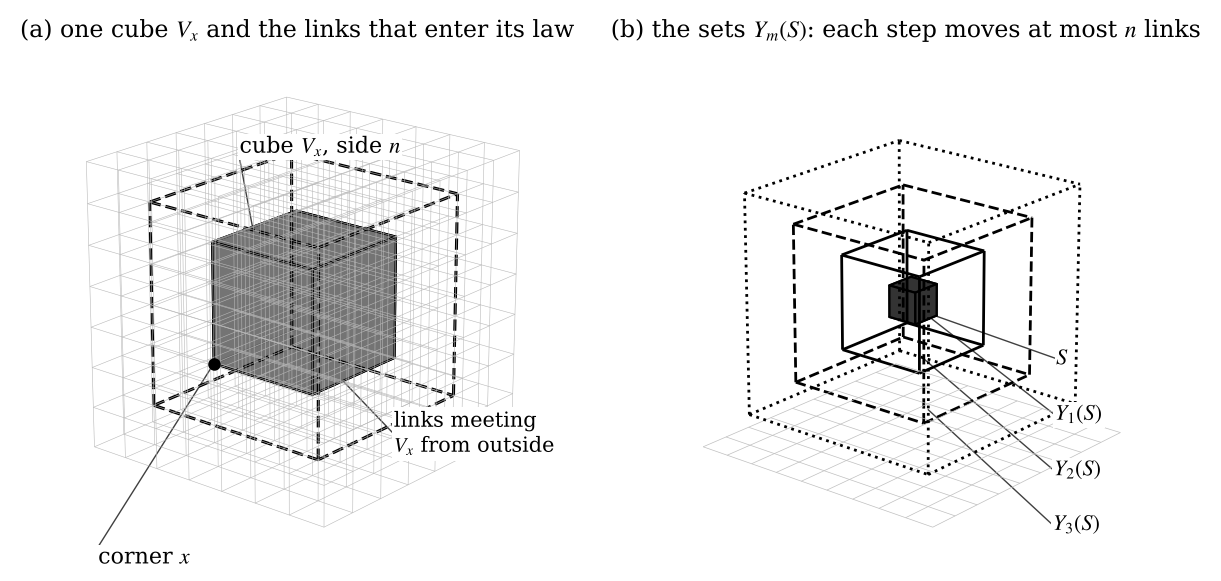
\includegraphics[width=\textwidth]{figures/fig_cube.png}
\caption{(a) The cube $V_x$ of side $n$ at $x$: its links are resampled by $\mathcal P_x$ from their conditional law given the boundary links $\partial V_x$, which lie in the plaquettes meeting $V_x$. (b) Finite speed: starting from a set $S$ of links, the sets $Y_1(S)\subset Y_2(S)\subset Y_3(S)$ of cubes reached by one, two and three steps of the relation $y\rightsquigarrow z$; each step moves the dependence by at most $n$ links in every coordinate, and at most $q_nn^4$ cubes feed one cube (Lemma~\ref{lem:speed}).}
\label{fig:cube}
\end{figure}

\begin{theorem}[decay from one cube]\label{thm:decay}
Suppose $\BP(n,\varpi)$ holds for $\mu$. Then $\varpi\le4$, and for bounded
real $f,g\in\mathcal A$ depending on the links of finite sets $S_f,S_g$ with
$d=d(S_f,S_g)\ge3n-2$,
\[
|\Cov_\mu(f,g)|\le\Bigl(e+\frac{k|S_f||S_g|}{64e^2}\Bigr)\|f\|_\infty\|g\|_\infty\,
e^{-\varpi k/(e^2q_n)},\qquad k=\Bigl\lfloor\frac{d+2}n\Bigr\rfloor-2 .
\]
In particular $|\Cov_\mu(f,g)|\le C(1+d)e^{-\varpi d/(e^2q_nn)}$ for every $d$,
with $C$ depending only on $|S_f|,|S_g|,\|f\|_\infty,\|g\|_\infty$.
\end{theorem}

\begin{proof}
\emph{The bound $\varpi\le4$.} Take $f=\ReTr U_p$ for one plaquette; since
$G\ne\{1\}$, $\ReTr g<N$ for $g\ne1$, and $\mu$ has a positive continuous
density with respect to Haar measure, so $\Var_\mu(f)>0$. Each
$I-\mathcal P_x$ is an orthogonal projection annihilating constants, so
$\mu((f-\mathcal P_xf)^2)\le\Var_\mu(f)$, and it vanishes unless $V_x$ contains
a link of $p$, which happens for at most $4n^4$ points $x$.

\emph{Spectral part.} On the functions of $\mathcal A$ with mean zero, $\mathcal K$
is self-adjoint with $0\le\mathcal K\le I$, and $\BP(n,\varpi)$ reads
$\ip h{(I-\mathcal K)h}\ge\epsilon\|h\|^2$ with $\epsilon=\varpi n^4/|\Lambda|$. So
$\|\mathcal K^Th\|_2\le e^{-\epsilon T}\|h\|_2$, and from
$f-\mu(f)=\mathcal K^T(f-\mu(f))+\sum_{t<T}\mathcal K^t(I-\mathcal K)f$,
\[
\Cov_\mu(f,g)=\ip{\mathcal K^T(f-\mu f)}{g-\mu g}+\sum_{t=0}^{T-1}
\ip{\mathcal K^tf}{(I-\mathcal K)g},
\]
whose first term is at most $e^{-\epsilon T}\|f\|_\infty\|g\|_\infty$.

\emph{Local part.} Let $Z_g=Y_1(S_g)$, so $|Z_g|\le n^4|S_g|$ and $(I-\mathcal K)g=
|\Lambda|^{-1}\sum_{x\in Z_g}(g-\mathcal P_xg)$; if $h$ does not depend on the links of
$V_x$ then $\ip h{g-\mathcal P_xg}=0$. Put $m_0=k-1$ and $Y=Y_{m_0}(S_f)$. A link
of $V_x$, $x\in Z_g$, lying in $S_f$ or in $\partial V_y$ with $y\in Y$ would join
base points of $S_f$ and $S_g$ at distance at most $n(m_0+3)-3\le n\lfloor
(d+2)/n\rfloor-3<d$, which is impossible: if $y\in Y_{m_0}(S_f)$ there is a
chain $y=y_j\rightsquigarrow\dots\rightsquigarrow y_1$, $j\le m_0$, with $y_1
\in Y_1(S_f)$, so $|y-y_1|_\infty\le n(m_0-1)$; a link of $\partial V_y$ has
base point in $y+[-1,n]^4$, a link of $V_{y_1}\cap S_f$ in $y_1+[0,n-1]^4$,
two links of $V_x$ have base points differing by at most $n-1$, and the
triangle inequality gives at most $n(m_0+1)-1\le n(m_0+3)-3$. So $\mathcal K_Y^tf$ does not depend on
the links of $V_x$, $x\in Z_g$, and by Lemma~\ref{lem:speed}
\[
\bigl|\ip{\mathcal K^tf}{(I-\mathcal K)g}\bigr|=\bigl|\ip{\mathcal K^tf-\mathcal K_Y^tf}
{(I-\mathcal K)g}\bigr|\le\frac{4|S_f||S_g|n^4}{q_n|\Lambda|}\|f\|_\infty\|g\|_\infty
\sum_{m\ge k}\frac{(q_n\tau_t)^m}{m!}.
\]
Summing over $t<T$ with $\tau=Tn^4/|\Lambda|$, the second term is at most
\[
\frac{4|S_f||S_g|\tau}{q_n}\,\|f\|_\infty\|g\|_\infty\sum_{m\ge k}
\frac{(q_n\tau)^m}{m!}.
\]

\emph{Choice of $T$.} Take $T=\lfloor k|\Lambda|/(e^2q_nn^4)\rfloor$, so that
$z=q_n\tau\le k/e^2$ and $\epsilon T\ge\varpi k/(e^2q_n)-1$, using $\varpi\le4$
and $|\Lambda|\ge4n^4$. Since $k!\ge(k/e)^k$, $\sum_{m\ge k}z^m/m!\le(ez/k)^ke^z\le
e^{-k(1-e^{-2})}$, and $\tau/q_n\le k/(256e^2)$. As $\varpi/(e^2q_n)<1-e^{-2}$,
both terms are bounded as stated. For the second form use $k>d/n-3$, and for
$d<3n-2$ the trivial bound $\|f\|_\infty\|g\|_\infty$.
\end{proof}

A \emph{torus limit} at $\beta$ is a state $\omega$ on the gauge-invariant local
functions of $\Z^4$ with $\omega(O)=\lim_j\mu_{L_j}(O)$ along some $L_j\to\infty$;
by compactness every sequence has a subsequence along which one exists.

\begin{corollary}[lattice gap]\label{cor:latticegap}
Let $\beta\ge0$ and suppose $\BP(n,\varpi)$ holds for $\mu_L$ for all $L$ in an
infinite set of even integers $L\ge2n+4$. Then every torus limit along this
set is invariant under translations, reflection positive, and its transfer
matrix has spectral gap at least
\[
m_n=\frac{\varpi}{e^2q_nn}\ge\frac{16\varpi}{625e^2n}.
\]
\end{corollary}

\begin{proof}
Translation invariance and reflection positivity are identities and
inequalities among finitely many local functions of $\mu_L$~\cite{OSei78}, and
pass to $\omega$. For a continuous gauge-invariant $F$ at positive times the
supports of $\vartheta(\bar F)$ and $\tau_tF$ are at distance $d$ with $|d-t|\le
c_F$, and Theorem~\ref{thm:decay} on $\Lambda_L$ gives $|\Cov_{\mu_L}(\vartheta(\bar
F),\tau_tF)|\le C_F(1+t)e^{-m_nt}$ uniformly in $L$. In the limit
$|\omega(\vartheta(\bar F)\tau_tF)-|\omega(F)|^2|\le C_F(1+t)e^{-m_nt}$, and
Proposition~\ref{prop:gapdecay}, applied with every $m<m_n$, gives the gap.
\end{proof}

\subsection{The continuum limit}

Let $a_k\to0$ be lattice spacings with $a_k=2^{-k}a_0$, and $\beta_k$ couplings.
Let $\omega_k$ be lattice states with transfer matrices $\mathbb T_k$ on spaces
$\mathcal H_k$ with vacua $\Omega_k$. Let $\mathcal T$ be a complex vector space of
test functions on $\R^4$ supported in $\{t>0\}$, and for each $k$ let $f\mapsto
O_k(f)$ be a linear map to gauge-invariant local observables at positive
times; the example is $O_k(f)=Z_k\sum_xa_k^4f(a_kx)\Phi(x)$ with a local field
$\Phi$ and a renormalisation constant $Z_k$.

\begin{definition}\label{def:limit}
A \emph{continuum limit} of $(\omega_k,O_k)$ is a Hilbert space $\mathcal H$ with
a unit vector $\Omega$, a self-adjoint $H\ge0$ with $H\Omega=0$, and a linear
map $\psi:\mathcal T\to\mathcal H$ with dense range such that for all
$f,g\in\mathcal T$ and dyadic $\tau\ge0$
\[
\ip{\psi(f)}{e^{-\tau H}\psi(g)}=\lim_k\omega_k\bigl(\vartheta(\overline{O_k(f)})
\,\tau_{\tau/a_k}O_k(g)\bigr),\qquad
\ip\Omega{\psi(f)}=\lim_k\omega_k(O_k(f)),
\]
over the $k$ with $\tau/a_k\in\Z$. It is \emph{nontrivial} if $\mathcal H\ne\C
\Omega$.
\end{definition}

The Osterwalder--Schrader reconstruction produces such a limit from
convergent renormalised Schwinger functions satisfying the
axioms~\cite{OS73,OS75}; the definition records only what is used below.

\begin{proof}[Proof of Theorem~\ref{thm:B}]
Let $\omega_k$ be torus limits at $\beta_k$ along the tori on which
$\BP(n_k,\varpi)$ holds. By Corollary~\ref{cor:latticegap}, $\mathbb T_k$ has gap
at least $16\varpi/(625e^2n_k)$ on $\Omega_k^\perp$. For $f\in\mathcal T$ put
$O=O_k(f)$ and $\varphi_k=\Psi_O-\omega_k(O)\Omega_k$. For dyadic $\tau$ and $k$
large, $t=\tau/a_k$ is an integer and $16\varpi t/(625e^2n_k)\ge\Delta\tau$ since
$n_ka_k\le\ell$, so
\[
\omega_k\bigl(\vartheta(\bar O)\tau_tO\bigr)-|\omega_k(O)|^2=\ip{\varphi_k}{\mathbb T_k^t
\varphi_k}\le e^{-\Delta\tau}\|\varphi_k\|^2 .
\]
Both sides converge by Definition~\ref{def:limit}: with $\varphi=\psi(f)-\ip\Omega
{\psi(f)}\Omega$, $\ip\varphi{e^{-\tau H}\varphi}\le e^{-\Delta\tau}\|\varphi\|^2$. These
vectors form a subspace dense in $\Omega^\perp$, and the inequality extends to
$\Omega^\perp$ and to all $\tau\ge0$ by continuity. For $\varphi\in\Omega^\perp$ with
spectral measure $\mu_\varphi$ of $H$ this says $\int e^{-\tau E}d\mu_\varphi(E)\le e^{-\Delta
\tau}\mu_\varphi([0,\infty))$ for all $\tau$, which forces $\mu_\varphi([0,\Delta-\eta])=0$
for every $\eta>0$. So $0$ is a simple eigenvalue and the spectrum on
$\Omega^\perp$ lies in $[\Delta,\infty)$, and is not empty if $\Omega^\perp\ne\{0\}$.
\end{proof}

The proof uses the cube condition only through the decay of two-point
functions of gauge-invariant observables, and the constant $\Delta$ depends on
$\varpi$ and $\ell$ alone.

\section{The bridge to a constructed continuum theory}\label{sec:bridge}

Theorem~\ref{thm:B} takes the lattice states first to infinite time extent
and only then to the continuum. A construction of a continuum theory may
proceed in a different order: on a symmetric torus of physical side $L_p$
the lattice spacing is sent to zero, and the side is sent to infinity
afterwards. The state at finite side is a thermal state at
temperature $1/L_p$, and its two-point functions carry contributions of
pairs of excited states that no single estimate on one scale controls
(Remark~\ref{rem:thermal}). This section proves that the cube condition on
cylinders, together with the hypothesis that the order of the two volume
limits does not matter, gives every theory constructed in this way, whose
outcome satisfies the Wightman axioms phase by phase, the mass gap of
Theorem~\ref{thm:B}, and that it forces the phase decomposition to be
trivial. No property of any particular construction is used: the three
hypotheses below are the whole input. Throughout, $G\subset\U(N)$ is a compact
simple group and the Wilson weight is $\exp(N\beta\sum_p\ReTr Q_p)$.

\subsection{Continuum families}\label{ssec:families}

For integers $L,M\ge2$ let $\Lambda_{L,M}=(\Z/L\Z)^3\times(\Z/M\Z)$ be the
cylinder with spatial side $L$ and time period $M$, with Wilson measure
$\mu_{L,M}$ at coupling $\beta$; $\Lambda_{L,L}=\Lambda_L$ is the symmetric
torus. A site is $(\vec x,t)$, a link is spatial or temporal, the time slice
$E_t$ is the set of spatial links with base time $t$, and the slab $[t,t']$
is the set of links with both ends at times in $[t,t']$.

\begin{definition}[continuum family]\label{def:family}
A continuum family consists of lattice spacings $a_N=1/N$, physical sides
$L_p\in\N$ with $L_p\to\infty$, couplings $\beta_{N,p}\ge0$, a countable set
$V$ of \emph{tokens}, and for every $N,p$ and $v\in V$ a complex function
$\Phi^{N,p}_v(x,Q)$ of a site $x$ of $\Lambda_{NL_p,M}$ and a configuration
$Q$, defined for every $M$ by the same formula, such that
\begin{enumerate}[label=\textup{(F\arabic*)},leftmargin=*]
\item $\Phi^{N,p}_v(x,\cdot)$ is continuous, gauge invariant, and depends only on
the links in $x+R_v$ for a finite set $R_v\subset\Z^4$ independent of $N,p$;
\item $\Phi^{N,p}_v(x+y,Q)=\Phi^{N,p}_v(x,\tau_{-y}Q)$ for every site $y$;
\item there is an involution $v\mapsto v^\vartheta$ of $V$ with
$\Phi^{N,p}_{v^\vartheta}(x,Q)=\overline{\Phi^{N,p}_v(\vartheta x,\vartheta Q)}$,
where $\vartheta$ is the reflection $t\mapsto-t$ of the time coordinate,
acting on configurations by $(\vartheta Q)_{(x,i)}=Q_{(\vartheta x,i)}$ for
spatial links and $(\vartheta Q)_{(x,0)}=Q_{(\vartheta x-e_0,0)}^{-1}$.\footnote{The
temporal link $(x,0)$ runs from $x$ to $x+e_0$; its image under $\vartheta$
runs from $\vartheta x$ to $\vartheta x-e_0$, which is the link
$(\vartheta x-e_0,0)$ traversed backwards, whence the inverse. With this
convention $\vartheta$ maps plaquette variables to plaquette variables of
the reflected plaquette, up to conjugation and inversion, so the Wilson
action and the Haar measure are invariant and $\vartheta$ is a measure
preserving involution of every $\Lambda_{L,M}$ with $M$ even, and of the
infinite cylinder.}
\end{enumerate}
\end{definition}

The insertions may carry renormalisation constants depending on $N$; no
bound on $\sup|\Phi^{N,p}_v|$ uniform in $N$ is assumed. For $m\ge1$ let
$D_m\subset(\R^4)^m$ be the open set of configurations of $m$ pairwise
distinct points, and let $\mathcal T_m$ be the complex-valued
$C^\infty$ functions with compact support in $D_m$; a \emph{cluster} is a
pair $(\mathbf v,t)$ with $\mathbf v\in V^m$ and $t\in\mathcal T_m$. For a
cluster supported in the box $(-L_p/2,L_p/2)^3\times(-M/(2N),M/(2N))$ the
lattice smear on $\Lambda_{NL_p,M}$ is
\begin{equation}\label{eq:smear}
S_{N,p,M}(\mathbf v,t)=a_N^{4m}\sum_{x_1,\dots,x_m}t(a_Nx_1,\dots,a_Nx_m)\,
\mu_{NL_p,M}\Bigl(\prod_{i=1}^m\Phi^{N,p}_{v_i}(x_i,\cdot)\Bigr),
\end{equation}
the sum over sites, with $a_Nx$ read in the box. Two clusters
$(\mathbf v,t)$, $(\mathbf v',t')$ with $t\in\mathcal T_m$, $t'\in\mathcal
T_{m'}$ have the product cluster $(\mathbf v\mathbf v',t\otimes t')$ when
$t\otimes t'$ is supported in $D_{m+m'}$. The reflected cluster is
$(\mathbf v^\vartheta,\Theta\bar t)$ with $(\Theta\bar t)(x_1,\dots,x_m)=
\overline{t(\vartheta x_1,\dots,\vartheta x_m)}$, and $\tau_\sigma t(x)=
t(x-\sigma e_0)$ is the translate by the Euclidean time $\sigma$. By (F3)
the smear of the reflected cluster is the lattice expectation of
$\vartheta\bar F$ when that of $(\mathbf v,t)$ is the expectation of $F$.

\begin{definition}[hypotheses on the family]\label{def:WUD}
Let $\ell>0$, $\varpi>0$ and $n_N\ge2$ with $n_Na_N\le\ell$.
\begin{enumerate}[label=\textup{(\Alph*)},leftmargin=*]
\item[\textup{(W)}] \emph{Wightman limit on symmetric tori.} There are a compact
metric space $X$ of \emph{phases} with a Borel probability measure $\nu$ of
full support, and for every $\chi\in X$ and every cluster a number
$S^\chi(\mathbf v,t)=\int t\,S^\chi_{\mathbf v}$ with $S^\chi_{\mathbf v}$ a
smooth function on $D_m$, continuous in $\chi$ at every point of $D_m$, such
that for every cluster
\[
\lim_{p\to\infty}\lim_{N\to\infty}S_{N,p,NL_p}(\mathbf v,t)=\int_X S^\chi(\mathbf v,t)
\,d\nu(\chi),
\]
with $\chi\mapsto S^\chi(\mathbf v,t)$ $\nu$-integrable, the inner limit along
$N$ in an arithmetic progression and the outer along a sequence of $p$, and
for $\nu$-almost every $\chi$ the functions
$S^\chi_{\mathbf v}$ are the Schwinger functions of a Wightman theory with
a unique vacuum, in the sense of Lemma~\ref{lem:wightman} below, in which
the field of $v^\vartheta$ is the adjoint of the field of $v$.
\item[\textup{(U)}] \emph{Order of the volume limits.} For every $N,p$ and
every cluster, $S^0_{N,p}(\mathbf v,t)=\lim_{M\to\infty}S_{N,p,M}(\mathbf v,t)$
satisfies
\[
\lim_{p\to\infty}\lim_{N\to\infty}S^0_{N,p}(\mathbf v,t)=\int_XS^\chi(\mathbf v,t)
\,d\nu(\chi)
\]
along the same progression and sequence.
\item[\textup{(D$_\ell$)}] \emph{The cube condition on cylinders.} For all large
$N$ and $p$ and every $M\ge2n_N+4$, $\BP(n_N,\varpi)$ holds for $\mu_{NL_p,M}$
at coupling $\beta_{N,p}$.
\end{enumerate}
\end{definition}

The limit in (U) exists by Lemma~\ref{lem:transfer}(v) below; (U) asserts
that the volume limit does not depend on whether the time extent is sent to
infinity before or after the lattice spacing. Hypothesis (W) lists what a
construction by scaling limits on symmetric tori delivers when it succeeds:
a fixed finite stencil for every insertion, gauge invariance, convergence of
the separated smears first in the mesh and then in the volume, a phase
measure of full support, continuity of the separated correlations in the
phase, and a Wightman theory with a unique vacuum for every phase, whose
Schwinger functions at Euclidean points are the phase correlations. The
reflection property (F3) and the identification of $v^\vartheta$ with the
adjoint field hold when the insertions are real and reflection symmetric, as
for Hermitian fields built from plaquettes. Hypothesis (U) is one instance
of the uniqueness of the volume limit, which such a construction need not
provide. A construction of this kind, for every compact simple group, is
claimed in the Lean~4 development~\cite{OAI26}, assessed in~\cite{YMG26};
neither is a refereed publication, the theorem below does not depend on
them, and they are cited only as the source of the shape of (W).

\begin{figure}[t]
\centering
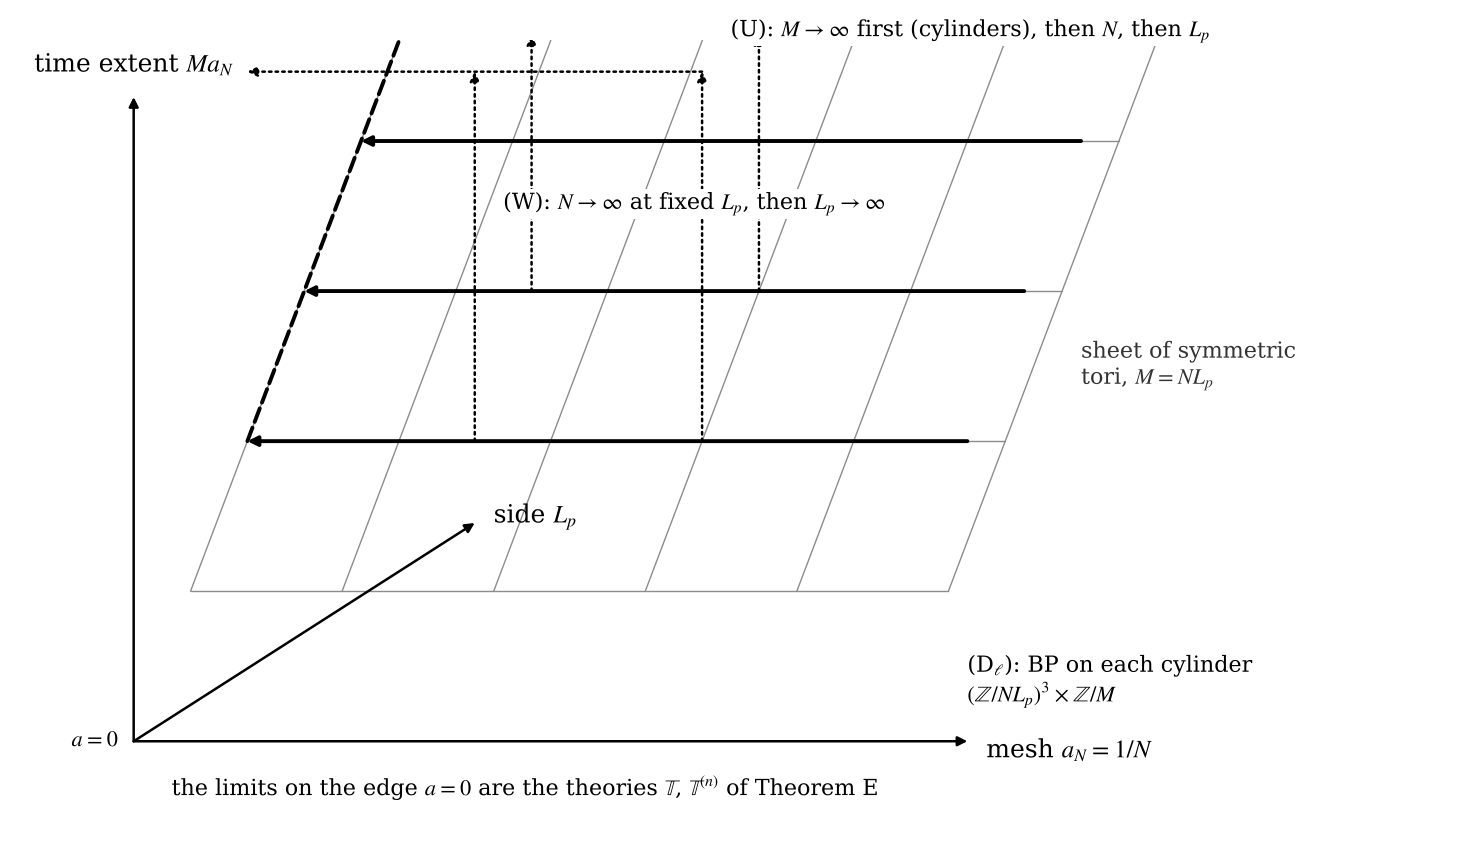
\includegraphics[width=\textwidth]{figures/fig_limits.png}
\caption{The two orders of the volume limits, in the space of mesh $a_N$, physical side $L_p$ and physical time extent $Ma_N$. The symmetric tori of (W) lie on the sheet where the time extent equals the side: the mesh is sent to zero at fixed $L_p$ along the sheet, then $L_p\to\infty$ along $a=0$ (solid and dashed arrows). The zero-temperature order sends the time extent to infinity first, on the cylinders where (D$_\ell$) is assumed, then the mesh, then the side (dotted arrows). Hypothesis (U), or its consequence of (Z) in Corollary~\ref{cor:Z}, is the statement that the two routes have the same end point.}
\label{fig:limits}
\end{figure}

\setcounter{mainthm}{4}
\begin{mainthm}[the bridge]\label{thm:E}
Let a continuum family satisfy \textup{(W)}, \textup{(U)} and
\textup{(D$_\ell$)}. Then $S^\chi$ does not depend on $\chi$, and the
Wightman theory of \textup{(W)} has Hamiltonian $H$ with
\[
\sigma(H)\subset\{0\}\cup[\Delta,\infty),\qquad\Delta=\frac{16\varpi}{625e^2\ell},
\]
with $0$ a simple eigenvalue.
\end{mainthm}
\setcounter{mainthm}{3}

The proof uses (W) only through the phase structure, the continuity in
$\chi$, the integrability of the phase correlations and the Wightman
property of the phases; the limit on symmetric tori enters through (U), or
through the weaker hypothesis (Z) of Section~\ref{ssec:thermalvacuum},
which implies the form of (U) that the proof needs. None of (W), (U), (Z)
or (D$_\ell$) is established in this paper for any four-dimensional family:
Theorem~\ref{thm:C} gives the cube condition at fixed strong coupling,
whereas (D$_\ell$) asks for it with $\varpi$ fixed and $n_N\le\ell N$ along
the couplings $\beta_{N,p}$ of a construction.

The proof occupies the rest of the section: the transfer matrix of a
cylinder (Sec.~\ref{ssec:transfermatrix}), its gap from the cube condition
(Sec.~\ref{ssec:cylindergap}), decay of the renormalised two-point functions
at zero temperature with a constant that survives the limit
(Sec.~\ref{ssec:zerotemp}), the Euclidean vectors of a Wightman theory
(Sec.~\ref{ssec:euclid}), and the assembly (Sec.~\ref{ssec:assembly}).

\subsection{The transfer matrix of a cylinder}\label{ssec:transfermatrix}

Fix $L$ and $\beta$. Let $\mathcal K=L^2(G^{E_0},\prod dQ_e)$ be the square
integrable functions of the spatial links of one time slice. For
configurations $Q,Q'$ of a slice and a family $U=(U_{\vec x})$ of temporal
link variables put
\[
S_s(Q)=\sum_{p\subset E_0}\ReTr Q_p,\qquad
S_0(Q,U,Q')=\sum_{\vec x,\,i}\ReTr\bigl(Q_{(\vec x,i)}U_{\vec x+e_i}
Q'^{\,*}_{(\vec x,i)}U^*_{\vec x}\bigr),
\]
the sums over the spatial plaquettes of the slice and over the timelike
plaquettes between two consecutive slices, and define the kernel
\begin{equation}\label{eq:transferkernel}
\mathbb T(Q,Q')=\int_{G^{(\Z/L\Z)^3}}\exp\Bigl(N\beta\bigl[\tfrac12S_s(Q)+\tfrac12S_s(Q')
+S_0(Q,U,Q')\bigr]\Bigr)\prod_{\vec x}dU_{\vec x}.
\end{equation}
For a function $F$ of the links of the slab $[0,w]$, $w\ge1$, let $\hat F$
be the operator on $\mathcal K$ with kernel
\begin{equation}\label{eq:slabkernel}
\begin{aligned}
\hat F(Q_0,Q_w)=\int&F(Q_0,U^{(0)},Q_1,\dots,U^{(w-1)},Q_w)\\
&\times\prod_{t=0}^{w-1}e^{N\beta[\frac12S_s(Q_t)+\frac12S_s(Q_{t+1})+S_0(Q_t,U^{(t)},Q_{t+1})]}
\prod_{t=1}^{w-1}dQ_t\prod_{t=0}^{w-1}dU^{(t)},
\end{aligned}
\end{equation}
and for $w=0$ let $\hat F$ be multiplication by $F$. Gauge transformations
$g=(g_{\vec x})$ of the slice act unitarily on $\mathcal K$ by $(R_gf)(Q)=
f(g\cdot Q)$.

\begin{lemma}[transfer matrix]\label{lem:transfer}
\begin{enumerate}[label=\textup{(\roman*)},leftmargin=*]
\item $\mathbb T$ is a self-adjoint Hilbert--Schmidt operator with a
continuous strictly positive kernel; its largest eigenvalue $\lambda_0>0$ is
simple, with a continuous eigenfunction $\Omega_0>0$, and every eigenfunction
with nonzero eigenvalue is gauge invariant. Every other eigenvalue has
modulus less than $\lambda_0$.
\item For $M\ge2$ the partition function of $\Lambda_{L,M}$ is $\Tr\mathbb T^M$.\footnote{The
spatial plaquettes of the slice $t$ carry weight $\frac12$ in each of the two
kernels $\mathbb T(Q_{t-1},Q_t)$ and $\mathbb T(Q_t,Q_{t+1})$, so they carry the
full Wilson weight exactly once around the cycle of $M$ slices, and the
temporal plaquettes between the slices $t$ and $t+1$ appear in $S_0(Q_t,
U^{(t)},Q_{t+1})$ only; the trace integrates over the $M$ slices and the
$M$ families of temporal links, which are all the links of $\Lambda_{L,M}$.}
\item Let $F$ be a bounded measurable function of the slab $[0,w]$ and $H$ one
of the slab $[0,w']$, and let $s\ge w$ and $M\ge s+w'$. Then
\[
\mu_{L,M}(F\,\tau_sH)=\frac{\Tr(\hat F\,\mathbb T^{s-w}\hat H\,\mathbb T^{M-s-w'})}
{\Tr\mathbb T^M}.
\]
\item The function $\vartheta\bar F$ is a function of the slab $[-w,0]$, and
for $s\ge0$ and $M\ge s+w+w'$
\[
\mu_{L,M}\bigl(\vartheta\bar F\,\tau_sH\bigr)=\frac{\Tr(\hat F^*\,\mathbb T^{s}
\hat H\,\mathbb T^{M-s-w-w'})}{\Tr\mathbb T^M}.
\]
\item For every bounded measurable function $F$ of a slab the limit
$\mu^0_{L}(F)=\lim_{M\to\infty}\mu_{L,M}(F)$ exists, and with $\Psi_F=
\lambda_0^{-w}\hat F\Omega_0$ and $\mathbb R=\mathbb T/\lambda_0$,
\[
\mu^0_L(\vartheta\bar F\,\tau_sH)=\ip{\Psi_F}{\mathbb R^s\Psi_H},\qquad
\mu^0_L(H)=\ip{\Omega_0}{\Psi_H}\qquad(s\ge0).
\]
\item If $F$ is gauge invariant then $R_g\hat F=\hat FR_g$ for every $g$.
\item If $\beta\ge0$ then $\mathbb T\ge0$ as an operator on $\mathcal K$.
\end{enumerate}
\end{lemma}

\begin{proof}
(i) The integrand of~\eqref{eq:transferkernel} is continuous and positive on
a compact space, so the kernel is continuous and strictly positive, and
$\mathbb T$ is Hilbert--Schmidt. Replacing $U_{\vec x}$ by $U_{\vec x}^{-1}$,
which preserves Haar measure, and using $\ReTr A=\ReTr A^*$ with the
cyclicity of the trace turns $S_0(Q,U,Q')$ into $S_0(Q',U,Q)$, so the kernel
is symmetric and $\mathbb T$ is self-adjoint. A simultaneous gauge
transformation $Q\mapsto g\cdot Q$, $Q'\mapsto g'\cdot Q'$ is absorbed by
$U_{\vec x}\mapsto g_{\vec x}^{-1}U_{\vec x}g'_{\vec x}$, so
$\mathbb T(g\cdot Q,g'\cdot Q')=\mathbb T(Q,Q')$; hence $\mathbb Tf$ is gauge
invariant for every $f$, and an eigenfunction with nonzero eigenvalue, being
in the range of $\mathbb T$, is gauge invariant and continuous. By Jentzsch's\footnote{Jentzsch's
theorem~\cite{Jen12}, in the form of~\cite[Ch.~V, \S6]{Sch74}: an integral
operator on $L^2(X,m)$, with $m$ a finite measure on a compact space $X$ and
a continuous kernel $k(x,y)>0$ everywhere, is compact, its spectral radius
$\lambda_0>0$ is an eigenvalue, simple, with an eigenfunction that is
strictly positive, and every other eigenvalue has modulus strictly less
than $\lambda_0$. Here $X=G^{E_0}$ with the product Haar measure, and the
kernel~\eqref{eq:transferkernel} is positive because the integrand is.}
theorem~\cite{Jen12}, in the form of~\cite[Thm.~V.6.6]{Sch74}, a compact
operator with a strictly positive kernel has its spectral radius as a simple
eigenvalue, with an almost everywhere positive eigenfunction, and every other
eigenvalue has smaller modulus; $\Omega_0=\lambda_0^{-1}\mathbb T\Omega_0$ is
continuous and strictly positive.

(ii) Write the Wilson weight of $\Lambda_{L,M}$ as the product over $t\in\Z/M\Z$
of $\exp(N\beta[\frac12S_s(Q_t)+\frac12S_s(Q_{t+1})+S_0(Q_t,U^{(t)},Q_{t+1})])$:
every spatial plaquette of slice $t$ appears with weight $\frac12$ in the
factors $t-1$ and $t$, and every timelike plaquette once. Integrating the
temporal links gives the kernel of $\mathbb T$ between consecutive slices, and
the integral over the slices is the trace of the $M$-fold product.

(iii) With the same factorisation, the slab $[0,w]$ contributes
$\hat F(Q_0,Q_w)$ after integrating its interior slices and temporal links,
the slab $[s,s+w']$ contributes $\hat H(Q_s,Q_{s+w'})$, and the remaining
$s-w$ and $M-s-w'$ factors contribute the powers of $\mathbb T$; when $s=w$
the shared slice $Q_w=Q_s$ is the integration variable of the composition
$\hat F\hat H$.

(iv) Under $\vartheta$ a temporal link from time $t$ to $t+1$ becomes the
link from $-t$ to $-t-1$, traversed backwards, which is the inversion in
(F3); the timelike plaquette weight is invariant, as in (i). So
$\vartheta\bar F$ is the function of the slab $[-w,0]$ whose kernel, in the
variables $(Q_{-w},Q_0)$, is $\overline{\hat F(Q_0,Q_{-w})}=\hat F^*(Q_{-w},Q_0)$.
Now apply (iii) to the slabs $[-w,0]$ and $[s,s+w']$.

(v) Let $P_0$ be the projection on $\Omega_0$ and $\mathbb R=\mathbb T/\lambda_0=
P_0+\mathbb S$ with $\|\mathbb S\|<1$ by (i). Since $\mathbb T^2$ is trace
class, $\|\mathbb S^{k}\|_1\le\|\mathbb S^2\|_1\|\mathbb S\|^{k-2}\to0$, so
$\Tr(A\mathbb R^{M-c})/\Tr\mathbb R^M\to\ip{\Omega_0}{A\Omega_0}$ for every
bounded $A$ and fixed $c$. Apply this to (iii) with $H=1$ for the existence of
the limit and to (iv) for the formula: $\Tr(\hat F^*\mathbb T^s\hat H
\mathbb T^{M-s-w-w'})/\Tr\mathbb T^M\to\lambda_0^{-s-w-w'}\ip{\Omega_0}
{\hat F^*\mathbb T^s\hat H\Omega_0}$.

(vi) The kernel~\eqref{eq:slabkernel} is invariant under simultaneous gauge
transformations of all slices of the slab, by the invariance of $F$ and the
substitution of (i) for the temporal links, so $\hat F(g\cdot Q_0,g\cdot Q_w)=
\hat F(Q_0,Q_w)$.

(vii) Put $f(g)=e^{N\beta\ReTr g}$ on $G$ and $c=N\beta\ge0$. Since $\ReTr g=
\frac12(\chi(g)+\overline{\chi(g)})$ with $\chi=\Tr$ the character of the
defining representation,
\[
f=\sum_{a,b\ge0}\frac{(c/2)^{a+b}}{a!\,b!}\,\chi^a\bar\chi^{\,b},
\]
uniformly on $G$, and $\chi^a\bar\chi^{\,b}$ is the character of
$(\C^N)^{\otimes a}\otimes(\overline{\C^N})^{\otimes b}$, a sum of irreducible
characters with nonnegative integer coefficients. Hence $f=\sum_\lambda
f_\lambda\chi_\lambda$ with $f_\lambda\ge0$, and as $\chi_\lambda(x^{-1}y)=
\sum_{a,b}\overline{D^\lambda_{ab}(x)}D^\lambda_{ab}(y)$ in a unitary basis,
$f(x^{-1}y)$ is a positive definite kernel on $G$; so is $f(xy^{-1})=
f(y^{-1}x)=f(x^{-1}y)$, by conjugation invariance and $\ReTr g=\ReTr g^{-1}$. By Schur's product theorem\footnote{The
entrywise product of two positive semidefinite matrices $(a_{ij})$,
$(b_{ij})$ is positive semidefinite, because it is the principal submatrix
of the tensor product $(a_{ij}b_{kl})$ on the diagonal pairs $(i,i)$, and the
tensor product of positive semidefinite matrices is positive semidefinite.
Applied to finite sections of continuous kernels this shows that the
product of positive definite kernels is positive definite.} the
kernel $K(Q,Q')=\prod_{e\in E_0}f(Q_eQ_e'^{\,*})$ is positive definite on
$G^{E_0}$, and being continuous it defines a nonnegative Hilbert--Schmidt
operator $K$ on $\mathcal K$. The substitution $Q'\mapsto U\cdot Q'$,
$(U\cdot Q')_{(\vec x,i)}=U_{\vec x}Q'_{(\vec x,i)}U^*_{\vec x+e_i}$, turns
$S_0(Q,U,Q')$ into $\sum\ReTr(Q_{(\vec x,i)}(U\cdot Q')^*_{(\vec x,i)})$, so
\[
\mathbb T=D\Bigl(\int K\circ R_{U}^{\,-1}\ \prod_{\vec x}dU_{\vec x}\Bigr)D
=D\,K\,\Pi\,D=D\,\Pi K\Pi\,D,
\]
where $D$ is multiplication by $e^{N\beta S_s/2}$, $\Pi=\int R_U\,dU$ is the
orthogonal projection on the gauge-invariant functions, and $K$ commutes with
every $R_g$ because $K(g\cdot Q,g\cdot Q')=K(Q,Q')$. Thus $\mathbb T=
(K^{1/2}\Pi D)^*(K^{1/2}\Pi D)\ge0$.
\end{proof}

The state $\mu^0_L$ is the zero-temperature state of the cylinder of
spatial side $L$: by (v) it is the expectation in the vector $\Omega_0$ of
the time-ordered products of slab operators, and $\mu_{L,M}$ is the
corresponding thermal state at temperature $1/M$.

\begin{figure}[t]
\centering
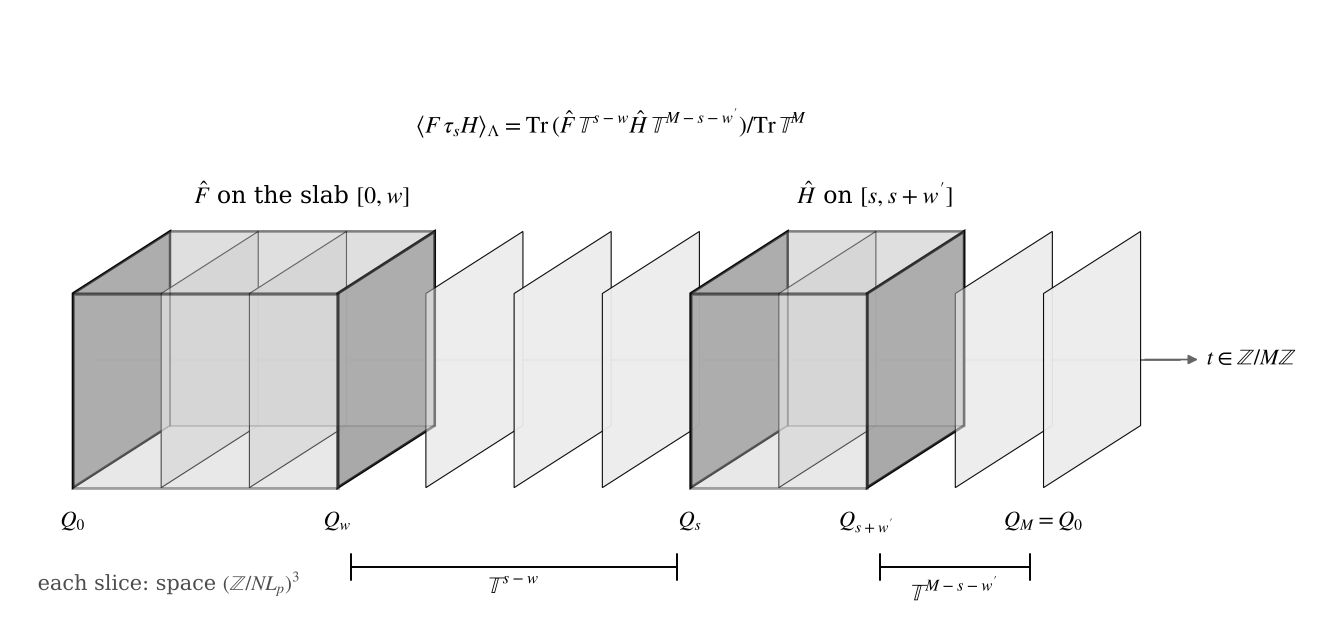
\includegraphics[width=\textwidth]{figures/fig_transfer.png}
\caption{The cylinder $\Lambda_{L,M}$ sliced in time. A function $F$ of the slab $[0,w]$ becomes the integral operator $\hat F$ on the slice space $\mathcal K$, a function $H$ of the slab $[s,s+w']$ becomes $\hat H$, and the time steps between the slabs are powers of the transfer matrix $\mathbb T$; the trace formula is Lemma~\ref{lem:transfer}(iii), and the reflected form, with $\hat F^*$, is Lemma~\ref{lem:transfer}(iv).}
\label{fig:transfer}
\end{figure}

\subsection{The gap of the transfer matrix from the cube condition}
\label{ssec:cylindergap}

\begin{proposition}[cylinder gap]\label{prop:cylindergap}
Let $n\ge2$, $\varpi>0$, $L\ge2n+4$, and suppose $\BP(n,\varpi)$ holds for
$\mu_{L,M}$ for every $M\ge2n+4$. Then every eigenvalue $\lambda\ne\lambda_0$ of
$\mathbb T$ satisfies
\[
\frac{|\lambda|}{\lambda_0}\le e^{-m_n},\qquad m_n=\frac{\varpi}{e^2q_nn}.
\]
\end{proposition}

\begin{proof}
Let $F$ be a real continuous gauge-invariant function of the slice $E_0$
with $|F|\le1$, depending on a set $S$ of links, and let $s\ge3n-2$ be
even. On $\Lambda_{L,M}$ with $M\ge2s$ the functions $F$ and $\tau_sF$ depend
on links whose base points differ by $s$ in time, so $d(S,\tau_sS)=s$; as
$s\ge3n-2$ and $n\ge2$, $M\ge2s\ge6n-4\ge2n+4$, so all sides of
$\Lambda_{L,M}$ are at least $2n+4$, $\BP(n,\varpi)$ holds for $\mu_{L,M}$,
and Theorem~\ref{thm:decay} gives
\[
\bigl|\mu_{L,M}(F\,\tau_sF)-\mu_{L,M}(F)^2\bigr|\le
\Bigl(e+\frac{k|S|^2}{64e^2}\Bigr)e^{-\varpi k/(e^2q_n)},\qquad
k=\Bigl\lfloor\frac{s+2}n\Bigr\rfloor-2 ,
\]
uniformly in $M$. Let $M\to\infty$: by Lemma~\ref{lem:transfer}(v) with
$w=w'=0$ and $\vartheta\bar F=F$, the left side becomes
$\ip{F\Omega_0}{\mathbb R^sF\Omega_0}-\ip{\Omega_0}{F\Omega_0}^2=
\sum_{j\ge1}r_j^s|\ip{\phi_j}{F\Omega_0}|^2$, where $(\phi_j)_{j\ge0}$ is an
orthonormal eigenbasis of $\mathbb T$ with real eigenvalues $\lambda_j=r_j
\lambda_0$, $\phi_0=\Omega_0$. As $s$ is even every term is nonnegative, and
$s/n-3<k\le s/n$, so for each $j\ge1$
\[
|r_j|^s\,|\ip{\phi_j}{F\Omega_0}|^2\le\Bigl(e+\frac{(s/n)|S|^2}{64e^2}\Bigr)
e^{3\varpi/(e^2q_n)}e^{-m_ns}.
\]
Letting $s\to\infty$ through even values gives $|r_j|\le e^{-m_n}$ whenever
$\ip{\phi_j}{F\Omega_0}\ne0$ for some such $F$. It remains to see that the
vectors $F\Omega_0$, $F$ real, span a dense subspace of the gauge-invariant
part of $\mathcal K$, which contains every $\phi_j$ with $\lambda_j\ne0$ by
Lemma~\ref{lem:transfer}(i). Let $h$ be gauge invariant and square
integrable. Since $\Omega_0$ is continuous, strictly positive and gauge
invariant, $h/\Omega_0$ is gauge invariant and square integrable for the
finite measure $\Omega_0^2\prod dQ_e$, and the continuous gauge-invariant
functions are dense in that space, because averaging a continuous
approximant over the compact gauge group preserves the approximation. If
$F_k\to h/\Omega_0$ there, then $\|F_k\Omega_0-h\|_{\mathcal K}\to0$; the real
and imaginary parts of $F_k$ are real continuous gauge-invariant functions.
\end{proof}

The proposition needs the cube condition on cylinders of every time period
and fixed spatial side: on a single symmetric torus the two-point function
of a bounded observable at separation $s\le M/2$ contains the thermal terms
$r_i^{M-s}r_j^{s}$, and a bound of the form $Ce^{-ms}$ for $s\le M/2$ at one
value of $M$ only gives $r_1\le e^{-m}(Cz)^{2/M}$ with $z=\Tr\mathbb R^M$, which tends to $e^{-m}$
as $M\to\infty$ at fixed coupling but not along a tuning in which the
coupling changes with $M$.

\subsection{Decay of renormalised two-point functions at zero temperature}
\label{ssec:zerotemp}

\begin{lemma}[gap to decay, with a surviving constant]\label{lem:gaptodecay}
Suppose every eigenvalue $\lambda\ne\lambda_0$ of $\mathbb T$ satisfies $|\lambda|
\le e^{-m}\lambda_0$. Let $F$ and $H$ be bounded measurable functions of the
slabs $[0,w]$ and $[0,w']$, let $\Psi'_F=\Psi_F-\ip{\Omega_0}{\Psi_F}\Omega_0$,
and put $C_F(s)=\mu^0_L(\vartheta\bar F\,\tau_sF)-|\mu^0_L(F)|^2=
\ip{\Psi'_F}{\mathbb R^s\Psi'_F}\ge0$. Then for all integers $s\ge s_1\ge0$,
\[
\bigl|\mu^0_L(\vartheta\bar F\,\tau_sH)-\overline{\mu^0_L(F)}\,\mu^0_L(H)\bigr|
\le e^{-m(s-s_1)}\sqrt{C_F(s_1)\,C_H(s_1)} .
\]
\end{lemma}

\begin{proof}
By Lemma~\ref{lem:transfer}(v) the left side is $|\ip{\Psi'_F}{\mathbb R^s
\Psi'_H}|$, since $\mathbb R\Omega_0=\Omega_0$ and $\Psi'_F\perp\Omega_0$. By
Lemma~\ref{lem:transfer}(vii), $\mathbb R\ge0$, so $\mathbb R^{s_1/2}$ is
defined by the functional calculus, and $\mathbb R^{s}=\mathbb R^{s_1/2}\,
\mathbb R^{s-s_1}\,\mathbb R^{s_1/2}$. The subspace $\Omega_0^\perp$ is
invariant under $\mathbb R$, on which $\|\mathbb R\|\le e^{-m}$, so the
Cauchy--Schwarz inequality gives $|\ip{\Psi'_F}{\mathbb R^s\Psi'_H}|\le
e^{-m(s-s_1)}\|\mathbb R^{s_1/2}\Psi'_F\|\,\|\mathbb R^{s_1/2}\Psi'_H\|$, and
$\|\mathbb R^{s_1/2}\Psi'_F\|^2=\ip{\Psi'_F}{\mathbb R^{s_1}\Psi'_F}=C_F(s_1)$.
\end{proof}

The point of the lemma is the constant. For a renormalised cluster the
norms $\|\Psi_F\|$, the suprema $\|F\|_\infty$ and the variances of $F$ under
the lattice measure diverge as $N\to\infty$, so the covariance bound of
Theorem~\ref{thm:decay} is useless for such $F$; the quantity $C_F(s_1)$ is
the connected two-point function of the cluster with its reflection at the
positive separation $s_1$, which under (U) converges to a Schwinger function
at separated points.

\subsection{Euclidean vectors of a Wightman theory}\label{ssec:euclid}

Let $(\mathcal H,\Omega,U)$ carry a Wightman theory in the sense
of~\cite[Ch.~3]{SW64}: a unitary representation $U(a,\Lambda)$ of the
Poincar\'e group with energy--momentum $P$ satisfying the spectrum condition
$\sigma(P)\subset\overline{V_+}$, a unique invariant unit vector $\Omega$,
and operator-valued tempered distributions $\Phi_v$, $v\in V$, on a common
dense invariant domain containing $\Omega$, covariant under $U$ and local,
with $\Omega$ cyclic for the polynomials in the fields, and with
$\Phi_{v^\vartheta}(f)=\Phi_v(\bar f)^*$ on the domain. Let $H=P^0\ge0$. We use
the metric $p\cdot z=p^0z^0-\vec p\cdot\vec z$ and $U(a)=e^{iP\cdot a}$, and the
forward tube
\[
\mathfrak T_m=\bigl\{z\in(\C^4)^m:\ \operatorname{Im}z_1\in V_+,\
\operatorname{Im}(z_{j+1}-z_j)\in V_+\ (1\le j<m)\bigr\}.
\]
A Euclidean point $x=(x_1,\dots,x_m)\in(\R^4)^m$ with times $0<\tau_1<\dots<
\tau_m$ corresponds to $\hat x=((i\tau_1,\vec x_1),\dots,(i\tau_m,\vec x_m))
\in\mathfrak T_m$.

\begin{lemma}[Euclidean vectors]\label{lem:wightman}
\begin{enumerate}[label=\textup{(\roman*)},leftmargin=*]
\item For $\mathbf v\in V^m$ there is a holomorphic function $\Psi_{\mathbf v}:
\mathfrak T_m\to\mathcal H$ whose boundary value as $\operatorname{Im}z\to0$
inside the tube is the vector-valued distribution $\Phi_{v_1}(x_1)\cdots
\Phi_{v_m}(x_m)\Omega$.
\item For a cluster $(\mathbf v,t)$ with $t$ supported in the configurations
with $0<\tau_1<\dots<\tau_m$, the vector $\psi(\mathbf v,t)=\int t(x)
\Psi_{\mathbf v}(\hat x)\,dx$ satisfies $\ip\Omega{\psi(\mathbf v,t)}=
\int t\,S_{\mathbf v}$ and, for $\sigma\ge0$ and a second such cluster,
\[
\ip{\psi(\mathbf v,t)}{e^{-\sigma H}\psi(\mathbf v',t')}=\int(\Theta\bar t\otimes
\tau_\sigma t')\,S_{\mathbf v^\vartheta\mathbf v'},\qquad
\mathbf v^\vartheta=(v_1^\vartheta,\dots,v_m^\vartheta),
\]
where $S_{\mathbf u}$ are the Schwinger functions, defined as follows. The
vacuum expectation $W_{\mathbf u}(x)=\ip\Omega{\Phi_{u_1}(x_1)\cdots
\Phi_{u_k}(x_k)\Omega}$ is the boundary value of a function
$W_{\mathbf u}(\zeta)$ holomorphic in the difference tube
\[
\mathfrak T'_k=\bigl\{\zeta\in(\C^4)^k:\ \operatorname{Im}(\zeta_{j+1}-\zeta_j)
\in V_+\ (1\le j<k)\bigr\},
\]
and $S_{\mathbf u}(x)=W_{\mathbf u}(\hat x)$ when $\tau_1<\dots<\tau_k$,
extended to the configurations with distinct times by permutation
symmetry.
\item The vectors $\psi(\mathbf v,t)$ of (ii), over all $m\ge1$, $\mathbf v$
and $t$, together with $\Omega$, span a dense subspace of $\mathcal H$.
\end{enumerate}
\end{lemma}

\begin{proof}
(i) The map $(f_1,\dots,f_m)\mapsto\Phi_{v_1}(f_1)\cdots\Phi_{v_m}(f_m)\Omega$
is multilinear and separately continuous from $\mathcal S(\R^4)^m$ to
$\mathcal H$, hence jointly continuous, and extends to a continuous linear map
$f\mapsto\Psi_{\mathbf v}(f)$ on $\mathcal S(\R^{4m})$ by the nuclear
theorem. Write $x_j=x_1+\xi_1+\dots+\xi_{j-1}$. Since $\Phi_{v_j}(x_j)\cdots
\Phi_{v_m}(x_m)\Omega=U(x_j)\Phi_{v_j}(0)\Phi_{v_{j+1}}(x_{j+1}-x_j)\cdots\Omega$
in the sense of distributions, the Fourier transform of $\Psi_{\mathbf v}$ in
the variable $x_1$ is supported in $\overline{V_+}$, and so is its Fourier
transform in each $\xi_j$, by the spectrum condition applied to the vector
to the right of $U(\xi_j)$. For every $\chi\in\mathcal H$ the scalar
distribution $\ip\chi{\Psi_{\mathbf v}(\cdot)}$ therefore has Fourier
transform supported in the closed convex cone $\overline{V_+}^{\,m}$ in these
variables, so it is the boundary value of a function holomorphic in
$\mathfrak T_m$~\cite[Thm.~2-8]{SW64}; the family of these distributions over
$\|\chi\|\le1$ is bounded in $\mathcal S'$, so the holomorphic functions are
uniformly bounded on compact subsets of the tube, and they define a weakly,
hence strongly, holomorphic $\Psi_{\mathbf v}:\mathfrak T_m\to\mathcal H$ with
$\ip\chi{\Psi_{\mathbf v}(z)}$ equal to these continuations.

(ii) The vacuum expectation $W_{\mathbf u}$ is translation invariant, and the
argument of (i) applied to the differences shows that it is the boundary
value of a function holomorphic in $\mathfrak T'_k$; for $x$ with increasing
times, $\hat x\in\mathfrak T'_k$ and $W_{\mathbf u}(\hat x)=\ip\Omega{\Psi_{\mathbf u}
(\hat x)}$ when the times are positive, by (i) and translation invariance, so
the first identity holds. For the second, let $z\in\mathfrak T_m$ and $z'\in
\mathfrak T_{m'}$. The function $(z,z')\mapsto\ip{\Psi_{\mathbf v}(z)}{
\Psi_{\mathbf v'}(z')}$ is antiholomorphic in $z$ and holomorphic in $z'$, and
by $\Phi_{v^\vartheta}(f)=\Phi_v(\bar f)^*$ its boundary value is the
distribution $W_{\check{\mathbf v}^\vartheta\mathbf v'}(x_m,\dots,x_1,y_1,\dots,
y_{m'})$, $\check{\mathbf v}^\vartheta=(v_m^\vartheta,\dots,v_1^\vartheta)$. The
map $(z,z')\mapsto(\bar z_m,\dots,\bar z_1,z'_1,\dots,z'_{m'})$ sends
$\mathfrak T_m\times\mathfrak T_{m'}$ into $\mathfrak T'_{m+m'}$: the
imaginary parts of the consecutive differences are $\operatorname{Im}(z_{j+1}
-z_j)$, $\operatorname{Im}z_1+\operatorname{Im}z'_1$ and $\operatorname{Im}
(z'_{j+1}-z'_j)$, all in $V_+$. Two functions holomorphic in $(\bar z,z')$ on
this product of tubes with the same distributional boundary
value coincide~\cite[Ch.~2]{SW64}, so
\[
\ip{\Psi_{\mathbf v}(z)}{\Psi_{\mathbf v'}(z')}=W_{\check{\mathbf v}^\vartheta\mathbf v'}
(\bar z_m,\dots,\bar z_1,z'_1,\dots,z'_{m'}).
\]
Next, $U(a)\Psi_{\mathbf v'}(z')=\Psi_{\mathbf v'}(z'+a)$ for real $a$ by
covariance; both sides are holomorphic in $a$ on the tube
$\operatorname{Im}a\in V_+$ with these boundary values, the left by the
spectrum condition and the right because $z'+a\in\mathfrak T_{m'}$, so they
agree there, and $e^{-\sigma H}\Psi_{\mathbf v'}(\hat y)=\Psi_{\mathbf v'}
(\widehat{\tau_\sigma y})$. At the Euclidean points $z=\hat x$, $z'=
\widehat{\tau_\sigma y}$ one has $\bar z_j=\widehat{\vartheta x_j}$, and the
times $-\tau_m<\dots<-\tau_1<\sigma+\tau'_1<\dots$ increase, so
\[
\ip{\Psi_{\mathbf v}(\hat x)}{e^{-\sigma H}\Psi_{\mathbf v'}(\hat y)}
=S_{\check{\mathbf v}^\vartheta\mathbf v'}(\vartheta x_m,\dots,\vartheta x_1,
\tau_\sigma y_1,\dots,\tau_\sigma y_{m'}).
\]
Integrate against $\bar t(x)t'(y)$ and substitute $u_i=\vartheta x_{m+1-i}$;
the permutation symmetry
\[
S_{\check{\mathbf v}^\vartheta\mathbf v'}(u_m,\dots,u_1,y)=S_{\mathbf v^\vartheta
\mathbf v'}(u_1,\dots,u_m,y)
\]
turns the result into $\int\overline{t(\vartheta u_1,\dots,\vartheta u_m)}\,
(\tau_\sigma t')(y)\,S_{\mathbf v^\vartheta\mathbf v'}(u,y)\,du\,dy$, which is
the claim.

(iii) Let $\chi\perp\Omega$ and $\chi\perp\psi(\mathbf v,t)$ for all clusters
of (ii). Then the
holomorphic function $\ip\chi{\Psi_{\mathbf v}(z)}$ vanishes on the open
subset $\{\hat x\}$ of the totally real submanifold $\{(i\tau_j,\vec x_j)\}
\cap\mathfrak T_m$, which has real dimension $4m$; after the complex-linear
change of coordinates $z^0_j\mapsto-iz^0_j$ this is an open subset of
$\R^{4m}$, so the function vanishes on the connected tube. Its boundary
value $\ip\chi{\Phi_{v_1}(x_1)\cdots\Phi_{v_m}(x_m)\Omega}$ then vanishes as a
distribution, for all $m$ and $\mathbf v$, so $\chi$ is orthogonal to the
polynomials in the fields applied to $\Omega$, which are dense, and to
$\Omega$ itself.
\end{proof}

\subsection{Proof of Theorem~\ref{thm:E}}\label{ssec:assembly}

\emph{Step 1: the lattice inequality.} Fix $N$ and $p$ large, put $L=NL_p$,
$n=n_N$ and $a=a_N$, and let $\mathbb T$ be the transfer matrix of the
cylinder of side $L$ at coupling $\beta_{N,p}$. Since $n_N\le\ell N$, one has
$L\ge2n_N+4$ as soon as $L_p\ge2\ell+1$ and $N\ge4$, which holds for $p$ and
$N$ large; so by (D$_\ell$) and Proposition~\ref{prop:cylindergap},
$\mathbb T$ has gap $m_n=\varpi/(e^2q_nn)$. Let $(\mathbf v,t)$ and
$(\mathbf v',t')$ be clusters with $t,t'$ supported in configurations whose
times lie in $(\delta,\omega)$, $0<\delta<\omega$, and let $\rho\ge0$ be such
that $R_v\subset\Z^3\times[-\rho,\rho]$ for the finitely many tokens $v$ of
$\mathbf v,\mathbf v'$, a link being in $x+R_v$ when its base point is. For
$N>\rho/\delta$ a site $x$ with $t(ax)\ne0$ has time $x^0\in(\delta N,\omega
N)$, so the links of $x+R_v$ have end points at times in $[x^0-\rho,x^0+\rho
+1]\subset[0,\lceil\omega N\rceil+\rho]$; hence the lattice functions
\[
F=a^{4m}\sum_xt(ax)\prod_i\Phi^{N,p}_{v_i}(x_i,\cdot),\qquad
H=a^{4m'}\sum_yt'(ay)\prod_j\Phi^{N,p}_{v'_j}(y_j,\cdot)
\]
are bounded, gauge invariant, and depend on the links of the slab
$[0,w]$ with $w=\lceil\omega N\rceil+\rho$. Let $\sigma\ge\sigma_1\ge1$ be integers.
Lemma~\ref{lem:gaptodecay} with $s=\sigma N$, $s_1=\sigma_1N$ gives
\begin{equation}\label{eq:latticeineq}
\bigl|\mu^0_L(\vartheta\bar F\,\tau_{\sigma N}H)-\overline{\mu^0_L(F)}\mu^0_L(H)\bigr|
\le e^{-m_nN(\sigma-\sigma_1)}\sqrt{C_F(\sigma_1N)C_H(\sigma_1N)},
\end{equation}
and $m_nN=\varpi/(e^2q_nna)\ge\Delta$ because $na\le\ell$ and $q_n\le625/16$.
Each quantity in~\eqref{eq:latticeineq} is a zero-temperature smear $S^0_{N,p}$
of a cluster: by (F3), $\vartheta\bar F=a^{4m}\sum_y(\Theta\bar t)(ay)\prod_i
\Phi^{N,p}_{v_i^\vartheta}(y_i,\cdot)$, and by (F2), $\tau_{\sigma N}H=a^{4m'}
\sum_y(\tau_\sigma t')(ay)\prod_j\Phi^{N,p}_{v'_j}(y_j,\cdot)$ since $\sigma N
\in\Z$; so $\mu^0_L(\vartheta\bar F\,\tau_{\sigma N}H)$ is the smear of
$c_1=(\mathbf v^\vartheta\mathbf v',\Theta\bar t\otimes\tau_\sigma t')$,
$\mu^0_L(F)$ and $\mu^0_L(H)$ those of $c_2=(\mathbf v,t)$ and $c_3=(\mathbf v',
t')$, and $C_F(\sigma_1N)$ is the smear of $c_4=(\mathbf v^\vartheta\mathbf v,
\Theta\bar t\otimes\tau_{\sigma_1}t)$ minus $|S^0_{N,p}(\mathbf v,t)|^2$. The product clusters are supported in
$D_{m+m'}$ because reflected and translated times are separated by at least
$2\delta$.

\emph{Step 2: the limit.} Let $N\to\infty$ along the progression and then
$p\to\infty$ along the sequence of (W). By (U) every smear
in~\eqref{eq:latticeineq} converges to the $\nu$-average of the corresponding
phase correlation. Writing $\bar S(\cdot)=\int_XS^\chi(\cdot)\,d\nu$ and
$\bar S^c(t,t';\sigma)=\bar S(\mathbf v^\vartheta\mathbf v',\Theta\bar t
\otimes\tau_\sigma t')-\overline{\bar S(\mathbf v,t)}\,\bar S(\mathbf v',t')$,
\begin{equation}\label{eq:limitineq}
|\bar S^c(t,t';\sigma)|\le e^{-\Delta(\sigma-\sigma_1)}\sqrt{\bar S^c(t,t;\sigma_1)
\,\bar S^c(t',t';\sigma_1)}
\end{equation}
for all integers $1\le\sigma_1\le\sigma$, the right side being nonnegative as a
limit of nonnegative numbers.

\emph{Step 3: the phases coincide.} For $\nu$-almost every $\chi$ the phase is
a Wightman theory, and by Lemma~\ref{lem:wightman}(ii) its own connected
function $S^{\chi,c}(t,t;\sigma)=\|e^{-\sigma H_\chi/2}\psi_\chi'\|^2\ge0$, with
$\psi'_\chi=\psi_\chi(\mathbf v,t)-\ip{\Omega_\chi}{\psi_\chi(\mathbf v,t)}
\Omega_\chi$. Hence
\[
\bar S^c(t,t;\sigma)=\int_XS^{\chi,c}(t,t;\sigma)\,d\nu(\chi)+\operatorname{Var}_\nu
\bigl(S^\chi(\mathbf v,t)\bigr)\ge\operatorname{Var}_\nu\bigl(S^\chi(\mathbf v,t)\bigr),
\]
the variance being finite because $|S^\chi(\mathbf v,t)|^2\le\|\psi_\chi
(\mathbf v,t)\|^2=S^\chi(\mathbf v^\vartheta\mathbf v,\Theta\bar t\otimes t)$ is
$\nu$-integrable by (W); while by~\eqref{eq:limitineq} with $t'=t$ the left
side tends to $0$ as $\sigma\to\infty$. So $S^\chi(\mathbf v,t)=\bar S(\mathbf v,t)$
for $\nu$-almost every $\chi$, for every cluster whose times are ordered in
some $(\delta,\omega)$. Fix $m$, $\mathbf v\in V^m$ and the open set
$\mathcal O=\{0<\tau_1<\dots<\tau_m\}\subset D_m$, and a countable set
$\mathcal D\subset C^\infty_c(\mathcal O)$ such that every $t\in C^\infty_c
(\mathcal O)$ is a uniform limit of elements of $\mathcal D$ supported in a
fixed compact subset of $\mathcal O$. As $V$ is countable, there is a
$\nu$-null set $X_1$ such that for $\chi\notin X_1$ the phase is a Wightman
theory and $S^\chi(\mathbf v,t)=\bar S(\mathbf v,t)$ for all $m$, $\mathbf v$
and $t\in\mathcal D$. For $\chi,\chi'\notin X_1$ the continuous function
$S^\chi_{\mathbf v}-S^{\chi'}_{\mathbf v}$ integrates to $0$ against every
$t\in\mathcal D$, hence against every $t\in C^\infty_c(\mathcal O)$, hence
vanishes on $\mathcal O$; by translation invariance in time and the
permutation symmetry of the Schwinger functions it vanishes at every
configuration with distinct times, and by continuity on $D_m$. Fix $\chi_0
\notin X_1$. For $x\in D_m$ the set $\{\chi:S^\chi_{\mathbf v}(x)=
S^{\chi_0}_{\mathbf v}(x)\}$ is closed by (W) and contains $X\setminus X_1$,
which is dense because $\nu$ has full support and $\nu(X_1)=0$; so it is
$X$. Thus $S^\chi=S^{\chi_0}$ for every $\chi$, $\bar S=S^{\chi_0}$, and
\eqref{eq:limitineq} holds for the Schwinger functions of the Wightman theory
of (W), call it $(\mathcal H,\Omega,H)$.

\emph{Step 4: the spectrum.} By Lemma~\ref{lem:wightman}(ii),
\eqref{eq:limitineq} with $t'=t$ reads, for the vector $\psi'=\psi(\mathbf v,t)
-\ip\Omega{\psi(\mathbf v,t)}\Omega\perp\Omega$,
\[
\ip{\psi'}{e^{-\sigma H}\psi'}\le e^{-\Delta(\sigma-\sigma_1)}\ip{\psi'}{e^{-\sigma_1H}\psi'}
\qquad(\sigma\ge\sigma_1\ge1\text{ integers}).
\]
If $\kappa$ is the spectral measure of $H$ at $\psi'$ and $0<\eta<\Delta$,
then $e^{-\sigma(\Delta-\eta)}\kappa([0,\Delta-\eta])\le e^{-\Delta(\sigma-\sigma_1)}
\kappa([0,\infty))$, so $\kappa([0,\Delta-\eta])\le e^{\Delta\sigma_1}\|\psi'\|^2
e^{-\eta\sigma}\to0$. Hence the spectral projection $E_H([0,\Delta-\eta])$
annihilates $\psi'$, that is $E_H([0,\Delta-\eta])\psi(\mathbf v,t)=
\ip\Omega{\psi(\mathbf v,t)}\Omega$, for every cluster with ordered times in
some interval $(\delta,\omega)$; every cluster of Lemma~\ref{lem:wightman}(ii)
is of this form. These vectors and $\Omega$, for which the identity is
trivial, span a dense subspace by Lemma~\ref{lem:wightman}(iii), so
$E_H([0,\Delta-\eta])$ is the projection on $\C\Omega$ for every $\eta>0$:
the spectrum of $H$ lies in $\{0\}\cup[\Delta,\infty)$ and $0$ is simple.
\qed

\begin{remark}[why the symmetric order needs \textup{(U)}]\label{rem:thermal}
On the symmetric torus the thermal two-point function of a slab function is
\[
\mu_{L,L}(\vartheta\bar F\,\tau_sF)=\frac{\lambda_0^{-2w}}{\Tr\mathbb R^L}
\sum_{i,j}r_i^{L-s-2w}r_j^{s}|\ip{\phi_j}{\hat F\phi_i}|^2,
\]
a sum of exponentials $e^{-s(E_j-E_i)}$ in which both signs of $E_j-E_i$
occur. It is convex, symmetric about $s=L/2-w$ when $\hat F$ is self-adjoint,
and it is not the Laplace transform of a positive measure on $[0,\infty)$
unless the terms with $i\ge1$ vanish. Those terms are bounded, by the log-convexity of
$\theta\mapsto\Tr(\mathbb T^{\theta}A\mathbb T^{1-\theta}A^*)$, by the
two-point functions at adjacent separation, but no bound on their sum that
is uniform in $N$ follows from the gap of $\mathbb T$ alone: it would require
a bound on $\sum_{i\ge1}r_i^{L}$, the thermal partition function of the
torus relative to its vacuum, uniformly in the lattice spacing, which is a
statement about the density of states up to the cutoff. Hypothesis (U)
replaces that estimate by the statement that the two orders of the volume
limits agree, and nothing in Theorem~\ref{thm:E} uses more. The next
subsection shows that the estimate is also sufficient: a bound on
$\sum_{i\ge1}r_i^L$ alone, hypothesis (Z) below, implies the form of (U)
that the proof uses.
\end{remark}

\begin{figure}[t]
\centering
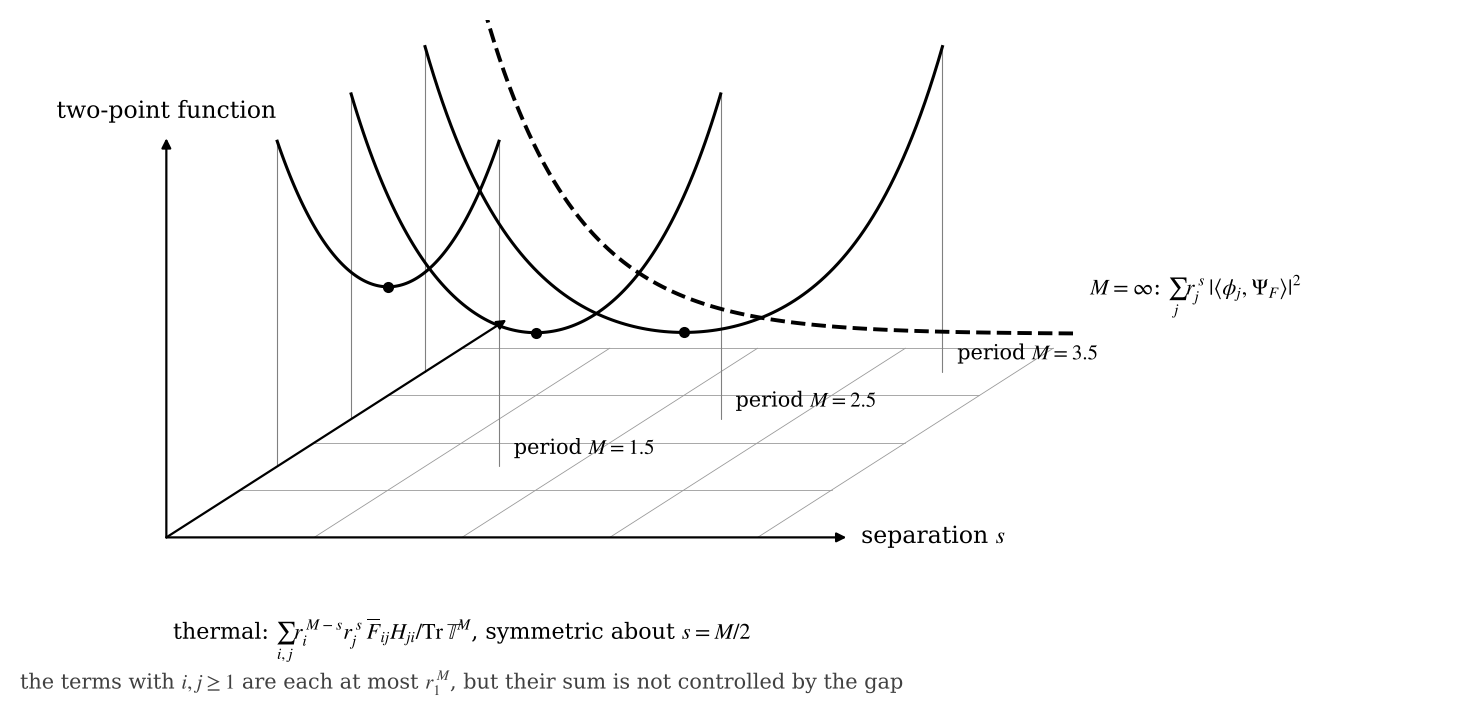
\includegraphics[width=\textwidth]{figures/fig_thermal.png}
\caption{Two-point functions of one slab observable on cylinders of physical period $M$ and at zero temperature ($M=\infty$), for one excited level of $\mathbb R$: the thermal function contains the terms $r_i^{M-s}r_j^{s}$ with both signs of $E_j-E_i$ and is symmetric about $s=M/2$ (Remark~\ref{rem:thermal}), while the zero-temperature function is the Laplace transform of a positive measure, which is what Lemma~\ref{lem:gaptodecay} uses. The terms with $i,j\ge1$ are each at most $r_1^{\,M}$, but their number is not controlled by the gap; Lemma~\ref{lem:thermaldiscrepancy} bounds their total by $\mathcal Z_L(M)-1$.}
\label{fig:thermal}
\end{figure}

\subsection{Thermal states against the vacuum}\label{ssec:thermalvacuum}

Fix $L$ and $\beta$, let $\mathbb T$, $\lambda_0$, $\Omega_0$ and $\mathbb R=
\mathbb T/\lambda_0$ be as in Lemma~\ref{lem:transfer}, and for $M\ge2$ put
\[
\mathcal Z_L(M)=\Tr\mathbb R^M=\frac{Z(\Lambda_{L,M})}{\lambda_0^M}\ \ge1,
\]
the partition function of $\Lambda_{L,M}$ relative to the vacuum of the
cylinder. By Lemma~\ref{lem:transfer}(i),(ii), $\lambda_0=\lim_{M\to\infty}
Z(\Lambda_{L,M})^{1/M}$, so $\mathcal Z_L(M)$ is determined by the Wilson
partition functions alone and involves no insertion.\footnote{In the
language of statistical mechanics, $-\log\lambda_0$ is the ground-state
energy of the cylinder Hamiltonian $H_L=-\log\mathbb T$ restricted to the
range of $\mathbb T$, $\log Z(\Lambda_{L,M})=\log\Tr e^{-MH_L}$ is minus $M$
times the free energy at temperature $1/M$, and $\log\mathcal Z_L(M)=
\log\Tr e^{-M(H_L-E_0)}$ is the thermal correction to the free energy, which
vanishes at zero temperature. Hypothesis (Z) is the statement that this
correction tends to zero when the temperature $1/L_p$ does, uniformly in
the mesh; for a theory with a gap $\Delta$ and finitely many states per
unit of energy and volume one expects $\mathcal Z-1$ of order
$L_p^4e^{-\Delta L_p}$.}

\begin{lemma}[thermal discrepancy]\label{lem:thermaldiscrepancy}
Let $G$ be a bounded measurable complex function of the slab $[0,w]$,
$w\ge0$, and let $M\ge2w+2$. Then $C_M(G)=\mu_{L,M}(\vartheta\bar G\,G)-
|\mu_{L,M}(G)|^2\ge0$, and
\[
\bigl|\mu_{L,M}(G)-\mu^0_L(G)\bigr|^2\le\bigl(\mathcal Z_L(M)-1\bigr)\,C_M(G),
\qquad
\mu^0_L(\vartheta\bar G\,G)\le\mathcal Z_L(M)\,\mu_{L,M}(\vartheta\bar G\,G).
\]
\end{lemma}

\begin{proof}
By Lemma~\ref{lem:transfer}(i),(vii) there is an orthonormal basis
$(\phi_i)_{i\ge0}$ of $\mathcal K$ of eigenvectors of $\mathbb R$, with
$\phi_0=\Omega_0$, $\mathbb R\phi_i=r_i\phi_i$, $r_0=1$ and $0\le r_i<1$
for $i\ge1$ (the eigenvectors for the nonzero eigenvalues completed by a
basis of $\ker\mathbb T$). Since $\mathbb T$ is Hilbert--Schmidt, $\mathbb R^k$ is
trace class for $k\ge2$, and $\mathcal Z_L(M)=\sum_ir_i^M=1+\varepsilon$ with
$\varepsilon=\sum_{i\ge1}r_i^M\ge0$.

Put $X=\lambda_0^{-w}\hat G$. For $w=0$ this is multiplication by $G$; for
$w\ge1$ the weights in~\eqref{eq:slabkernel} are positive and with $G=1$
they give the kernel of $\mathbb T^w$, so $|\hat G(Q,Q')|\le\|G\|_\infty
\mathbb T^w(Q,Q')$ and $\hat G$ is Hilbert--Schmidt. In both cases $X$ is
bounded, and $X\mathbb R^{M-w}$, $X^*X\mathbb R^{M-2w}$ are trace class because
$M-2w\ge2$. Lemma~\ref{lem:transfer}(iii) with $H=1$, $w'=0$, $s=w$,
Lemma~\ref{lem:transfer}(iv) with $F=H=G$, $s=0$, and
Lemma~\ref{lem:transfer}(v) give, with $X_{ii}=\ip{\phi_i}{X\phi_i}$,
\begin{equation}\label{eq:thermaltraces}
\begin{gathered}
\mathcal Z_L(M)\,\mu_{L,M}(G)=\sum_ir_i^{M-w}X_{ii},\qquad
\mu^0_L(G)=X_{00},\\
\mathcal Z_L(M)\,\mu_{L,M}(\vartheta\bar G\,G)=\sum_ir_i^{M-2w}\|X\phi_i\|^2.
\end{gathered}
\end{equation}
The term $i=0$ of the second identity is $\|X\Omega_0\|^2=\mu^0_L(\vartheta
\bar G\,G)$ by Lemma~\ref{lem:transfer}(v), which gives the second
inequality of the lemma.

Let $c=X_{00}$ and $G'=G-c$. The constant $c$ on the slab $[0,w]$ has
operator $c\,\mathbb T^w$, so $X'=\lambda_0^{-w}\hat G'=X-c\,\mathbb R^w$ and
$X'_{00}=0$, while $D=\mu_{L,M}(G)-\mu^0_L(G)=\mu_{L,M}(G')-\mu^0_L(G')=
\mu_{L,M}(G')$. By~\eqref{eq:thermaltraces} for $G'$, the Cauchy--Schwarz
inequality over $i\ge1$ with the weights $r_i^{M-w}=r_i^{M/2}r_i^{M/2-w}$, and
$|X'_{ii}|\le\|X'\phi_i\|$,
\begin{multline*}
\mathcal Z_L(M)\,|D|=\Bigl|\sum_{i\ge1}r_i^{M/2}\,r_i^{M/2-w}X'_{ii}\Bigr|
\le\varepsilon^{1/2}\Bigl(\sum_{i\ge1}r_i^{M-2w}\|X'\phi_i\|^2\Bigr)^{1/2}\\
\le\varepsilon^{1/2}\bigl(\mathcal Z_L(M)\,\mu_{L,M}(\vartheta\bar G'G')\bigr)^{1/2}.
\end{multline*}
The torus measure is invariant under $\vartheta$, so $\mu_{L,M}(\vartheta
\bar G)=\overline{\mu_{L,M}(G)}$, and expanding the product,
\begin{align*}
\mu_{L,M}(\vartheta\bar G'G')&=\mu_{L,M}(\vartheta\bar G\,G)-2\Re\bigl(\bar c\,
\mu_{L,M}(G)\bigr)+|c|^2\\&=C_M(G)+|\mu_{L,M}(G)-c|^2=C_M(G)+|D|^2 .
\end{align*}
Hence $|D|^2\le\frac{\varepsilon}{1+\varepsilon}\bigl(C_M(G)+|D|^2\bigr)$,
that is $|D|^2\le\varepsilon\,C_M(G)$. Finally $C_M(G)=\mu_{L,M}\bigl(
\vartheta\overline{G''}\,G''\bigr)$ with $G''=G-\mu_{L,M}(G)$, by the same
expansion, and the second identity of~\eqref{eq:thermaltraces} applied to
$G''$ shows that this is nonnegative.
\end{proof}

The inequality is sharp: for $\mathcal K=\C^2$, $\mathbb R=\operatorname{diag}(1,r)$,
$w=0$ and $G=\operatorname{diag}(x_0,x_1)$ one has $D=r^M(x_1-x_0)/(1+r^M)$,
$\mathcal Z-1=r^M$ and $C_M=r^M(x_1-x_0)^2/(1+r^M)^2$, so $|D|^2=(\mathcal Z-1)C_M$.
The lemma uses no gap, and no bound on $G$ beyond boundedness at fixed $N$:
the renormalisation constants of the insertions cancel between the two
sides. Conversely, no bound on the thermal correction follows from the gap
and operator norms alone: for $m>0$, $M\ge1$ and $c\in(0,1)$, let
$d=\lceil ce^{mM}/(1-c)\rceil$, $r=(c/((1-c)d))^{1/M}\le e^{-m}$, $\mathbb R=
\operatorname{diag}(1,r,\dots,r)$ on $\C^{1+d}$ and $X=I-P_{\Omega_0}$; then
$\Tr(X\mathbb R^M)/\Tr\mathbb R^M=dr^M/(1+dr^M)=c$ while $\ip{\Omega_0}{X\Omega_0}
=0$. The quantity $\mathcal Z_L(M)-1$ is therefore exactly the missing
information of Remark~\ref{rem:thermal}.

\begin{definition}\label{def:Zw}
For a continuum family put $\mathcal Z_{N,p}=\mathcal Z_{NL_p}(NL_p)$ at coupling
$\beta_{N,p}$, the partition function of the symmetric torus
$\Lambda_{NL_p}$ relative to the vacuum of the cylinder of the same spatial
side.
\begin{enumerate}[leftmargin=*]
\item[\textup{(Z)}] \emph{Vacuum dominance on the symmetric torus.}
$\displaystyle\lim_{p\to\infty}\limsup_{N\to\infty}\bigl(\mathcal Z_{N,p}-1\bigr)=0$,
the limits along the progression and the sequence of \textup{(W)}.
\item[\textup{(U$_w$)}] \emph{Weak order of the volume limits.} For every
cluster,
\[
\lim_{p\to\infty}\limsup_{N\to\infty}\Bigl|S^0_{N,p}(\mathbf v,t)
-\int_XS^\chi(\mathbf v,t)\,d\nu(\chi)\Bigr|=0 .
\]
\end{enumerate}
\end{definition}

Hypothesis (U) implies (U$_w$); (U$_w$) does not require the inner limit of
$S^0_{N,p}$ to exist. Hypothesis (Z) is one number per $(N,p)$, with no
insertion and no renormalisation: it says that the free energy of the
symmetric torus is its time extent times the free energy per unit time of
the cylinder, up to $o(1)$, uniformly in the mesh. For a gapped theory with
finite thermodynamics one expects $\mathcal Z_{N,p}-1$ of order
$L_p^4e^{-\Delta L_p}$; (Z) is not proved here for any four-dimensional
family.

\begin{proposition}[vacuum dominance gives the order of the limits]
\label{prop:ZgivesU}
Let a continuum family satisfy \textup{(W)}. Let $(\mathbf v,t)$ be a cluster
with $t$ supported in configurations whose times lie in $(-T_0,T_0)$, put
$\sigma_0=\lceil T_0\rceil+1\in\N$, $t_0=\tau_{\sigma_0}t$, and let
$c^\vartheta=(\mathbf v^\vartheta\mathbf v,\Theta\bar t_0\otimes t_0)$.
Then for all $p$ with $L_p>4T_0+6$ and all large $N$,
\begin{equation}\label{eq:SminusS0}
\bigl|S_{N,p,NL_p}(\mathbf v,t)-S^0_{N,p}(\mathbf v,t)\bigr|^2\le
(\mathcal Z_{N,p}-1)\Bigl(S_{N,p,NL_p}(c^\vartheta)-\bigl|S_{N,p,NL_p}(\mathbf v,t)
\bigr|^2\Bigr).
\end{equation}
Consequently \textup{(W)} and \textup{(Z)} imply \textup{(U$_w$)}.
\end{proposition}

\begin{proof}
\emph{Translation.} Since $\sigma_0N\in\Z$, the translation by $\sigma_0N$
time steps is a bijection of the sites of every $\Lambda_{NL_p,M}$. By (F2)
and the invariance of $\mu_{NL_p,M}$ and of $\mu^0_{NL_p}$ under lattice
translations, $S_{N,p,M}(\mathbf v,t_0)=S_{N,p,M}(\mathbf v,t)$ and
$S^0_{N,p}(\mathbf v,t_0)=S^0_{N,p}(\mathbf v,t)$, the box reading being
consistent because $t$, $t_0$ and $\Theta\bar t_0$ are supported in the box
when $L_p>4T_0+6$. The times of $t_0$ lie in $(1,\omega)$ with
$\omega=2T_0+2$.

\emph{Slab function.} Let $\rho$ bound the time extent of the stencils $R_v$,
and let $N>\rho$ be so large that $NL_p\ge2(\lceil\omega N\rceil+\rho)+2$,
which is possible since $L_p>2\omega$. The lattice function
$G=a^{4m}\sum_xt_0(ax)\prod_i\Phi^{N,p}_{v_i}(x_i,\cdot)$ is bounded, by (F1)
and compactness, and depends on the slab $[0,w]$ with $w=\lceil\omega N
\rceil+\rho$; moreover $S_{N,p,NL_p}(\mathbf v,t)=\mu_{NL_p,NL_p}(G)$,
$S^0_{N,p}(\mathbf v,t)=\mu^0_{NL_p}(G)$, and by (F3), as in Step~1 of
Section~\ref{ssec:assembly}, $\mu_{NL_p,NL_p}(\vartheta\bar G\,G)=
S_{N,p,NL_p}(c^\vartheta)$; the cluster $c^\vartheta$ is supported in $D_{2m}$
since reflected and original times are separated by at least $2$, and in
the box. Lemma~\ref{lem:thermaldiscrepancy} with $L=M=NL_p$
gives~\eqref{eq:SminusS0}.

\emph{Limit.} By (W) applied to $c^\vartheta$ and to $(\mathbf v,t)$, the
second factor on the right of~\eqref{eq:SminusS0} converges as $N\to\infty$,
for every large $p$, to a number $k_p$, and $k_p\to\int_XS^\chi(c^\vartheta)
\,d\nu-|\int_XS^\chi(\mathbf v,t)\,d\nu|^2<\infty$. Hence
$\limsup_N|S^0_{N,p}-S_{N,p,NL_p}|\le(\limsup_N(\mathcal Z_{N,p}-1))^{1/2}
k_p^{1/2}$, which tends to $0$ as $p\to\infty$ by (Z); since
$\lim_p\lim_NS_{N,p,NL_p}(\mathbf v,t)=\int_XS^\chi(\mathbf v,t)\,d\nu$ by (W),
(U$_w$) follows.
\end{proof}

\begin{corollary}\label{cor:Z}
The proof of Theorem~\ref{thm:E} remains valid with \textup{(U)} replaced
by \textup{(U$_w$)}. Hence a continuum family satisfying \textup{(W)},
\textup{(Z)} and \textup{(D$_\ell$)} has the conclusion of
Theorem~\ref{thm:E}: $S^\chi$ does not depend on $\chi$, and
$\sigma(H)\subset\{0\}\cup[\Delta,\infty)$ with $\Delta=16\varpi/(625e^2\ell)$
and $0$ simple.
\end{corollary}

\begin{proof}
Step~1 is a statement at fixed $N,p$ and uses only (D$_\ell$). In Step~2
write $x_{N,p}(c)=S^0_{N,p}(c)$ and $x(c)=\int_XS^\chi(c)\,d\nu$ for a
cluster $c$; by (U$_w$), $\eta_p(c)=\limsup_N|x_{N,p}(c)-x(c)|\to0$. The
quantities in~\eqref{eq:latticeineq} are $A_{N,p}=x_{N,p}(c_1)-\overline{
x_{N,p}(c_2)}x_{N,p}(c_3)$, $B_{N,p}=x_{N,p}(c_4)-|x_{N,p}(c_2)|^2\ge0$ and
the analogous $C_{N,p}\ge0$ for $t'$, with $c_1,\dots,c_4$ the clusters of
Step~1; let $A$, $B$, $C$ be the same expressions in $x$. From
$|yy'-zz'|\le|y-z||y'|+|z||y'-z'|$ and the boundedness of the $x_{N,p}$ along
the progression (they converge up to $\eta_p$), $\limsup_N|A_{N,p}-A|\le
\eta_p$, and similarly for $B$ and $C$, with $\eta_p\to0$. Hence $B,C\ge
-\eta_p$ for every large $p$, so $B,C\ge0$, and
\[
|A|\le\limsup_N|A-A_{N,p}|+e^{-\Delta(\sigma-\sigma_1)}\limsup_N\sqrt{B_{N,p}
C_{N,p}}\le\eta_p+e^{-\Delta(\sigma-\sigma_1)}\sqrt{(B+\eta_p)(C+\eta_p)},
\]
using $e^{-m_nN(\sigma-\sigma_1)}\le e^{-\Delta(\sigma-\sigma_1)}$. Letting
$p\to\infty$ gives~\eqref{eq:limitineq}; Steps~3 and~4 use
only~\eqref{eq:limitineq} and (W). The second statement follows from
Proposition~\ref{prop:ZgivesU}.
\end{proof}

\begin{lemma}\label{lem:Zmonotone}
$M\mapsto\mathcal Z_L(M)-1=\sum_{i\ge1}r_i^M$ is nonincreasing and
log-convex on $\{M\ge2\}$. If every eigenvalue $\lambda\ne\lambda_0$ of
$\mathbb T$ satisfies $|\lambda|\le e^{-m}\lambda_0$, then $\mathcal Z_L(M)-1
\le e^{-m(M-M')}(\mathcal Z_L(M')-1)$ for $M\ge M'\ge2$. In particular, under
\textup{(D$_\ell$)}, for integers $2\le b\le L_p$ and large $N$,
\[
\mathcal Z_{N,p}-1\le e^{-\Delta(L_p-b)}\bigl(\mathcal Z_{NL_p}(bN)-1\bigr).
\]
\end{lemma}

\begin{proof}
Each $r_i\in[0,1)$ for $i\ge1$, and a sum of exponentials $\sum_ie^{M\log r_i}$
is nonincreasing and log-convex in $M$. Under the gap, $r_i^M\le
e^{-m(M-M')}r_i^{M'}$. By Proposition~\ref{prop:cylindergap} and
(D$_\ell$), $m=m_{n_N}$ with $m_{n_N}N\ge\Delta$, as in Step~1 of
Section~\ref{ssec:assembly}.
\end{proof}

Thus (Z) follows from a bound on the relative partition function at the
higher temperature $1/b$ that grows slower than $e^{\Delta(L_p-b)}$.
Hypothesis (D$_\ell$) can likewise be replaced by the slab decorrelation of
Theorem~\ref{thm:D}, through its form on cylinders.

\begin{proposition}[the bridge from the slab decorrelation]\label{prop:bridgeM}
Let a continuum family satisfy \textup{(W)} and \textup{(U)}, or \textup{(W)}
and \textup{(Z)}, with the inner limits along the progression $\{N_0+kP\}$.
Let $K_0$ be a prime not dividing $P$, let $\mathcal N=\{N_0+kP\}\cap K_0\Z$,
and for $N\in\mathcal N$ put $d_N=N/K_0$ and $n_N=2d_N-1$, so that $n_Na_N<
\ell=2/K_0$. Suppose there are $0\le c<\frac12$ and $m\ge4$ with $m-1\ge
148/(1-2c)^4$ such that $(\mathrm M_{d_N,m}(c))$ holds for the Wilson weight
at $\beta_{N,p}$ for all large $N\in\mathcal N$ and all large $p$. Then the
conclusion of Theorem~\ref{thm:E} holds with
\[
\Delta=\frac{(1-2c)^4K_0}{2500\,e^2}.
\]
\end{proposition}

\begin{proof}
Since $K_0\nmid P$, the congruence $N_0+kP\equiv0\pmod{K_0}$ has a solution,
and $\mathcal N$ is an arithmetic progression of difference $K_0P$, a
subsequence of the original one; so (W) and (U), or (Z), hold along it with
the same limits. For $N\ge2K_0$ one has $d_N\ge2$ and $n_Na_N=(2N/K_0-1)/N<
\ell$; also $d_N\mid NL_p$, and $NL_p\ge2md_N$ once $K_0L_p\ge2m$. By
Corollary~\ref{cor:cylinders}, $\BP(n_N,\varpi)$ with $\varpi=(1-2c)^4/32$
holds for $\mu_{NL_p,M}$ for every $M\in d_N\Z$ with $M\ge2md_N$, and each
such $M$ is at least $2n_N+4$. In the proof of Theorem~\ref{thm:E},
(D$_\ell$) enters only in Step~1, through Proposition~\ref{prop:cylindergap},
whose proof uses $\BP(n,\varpi)$ on $\Lambda_{L,M}$ for $M\ge2s$ and then
lets $M\to\infty$, a limit that exists along every sequence by
Lemma~\ref{lem:transfer}(v); so the cylinders with $M\in d_N\Z$ suffice, and
$\mathbb T$ has gap $m_n=\varpi/(e^2q_nn)$. Steps~2 to~4 are unchanged, or
replaced by Corollary~\ref{cor:Z} under (Z). The gap is $16\varpi/(625e^2
\ell)=(1-2c)^4K_0/(2500e^2)$.
\end{proof}

The proposition replaces the cube condition on cylinders by the slab
decorrelation at the physical separation $(d_N-1)a_N\approx1/(2K_0)$,
uniform in the boundary condition, which is the form in which
Section~\ref{sec:weak} discusses the remaining hypothesis; none of (W), (U),
(Z) or $(\mathrm M_{d_N,m}(c))$ along a tuning is proved here. What
the cube condition does not give is a bound of this kind: (Z) is a statement
per unit of physical volume, while Theorem~\ref{thm:decay} controls each
local term of $\log\mathcal Z$ by a constant per lattice link or block,
with sup-norm factors that grow with $N$. Whether (U) implies (Z) is not
known to us; whether (Z) holds for Yang--Mills is open, and nothing in this
subsection bears on (W) or on (D$_\ell$). Section~\ref{ssec:layers} shows
what $(\mathrm M_{d_N,m}(c))$ asks beyond the gap it produces: computed in
the vacuum of the cylinder instead of under an arbitrary boundary
condition, the same maximal correlation equals $e^{-m_{\mathrm{lat}}s}$
exactly (Proposition~\ref{prop:vacuumlayers}).

Two facts delimit what a proof of (Z) can use. The first is that (Z) is
not determined by the data that (W) and the gap provide: the correlation
functions of the observables at every period and at zero temperature, the
gap, the positivity of the transfer operator and the uniqueness of its
leading eigenvector. The second is that the agreement of the two orders of
limits for all local correlations, hypothesis (U), does not imply (Z) in the
class of reflection-positive lattice models with a gapped transfer matrix.

\begin{proposition}[decoupled sectors]\label{prop:invisible}
Let $\mathbb R\ge0$ be a self-adjoint operator on a separable Hilbert space
$\mathcal K$ with $\mathbb R^2$ of trace class, such that $1$ is a simple
eigenvalue of $\mathbb R$ with unit eigenvector $\Omega$ and
$\|\mathbb R|_{\Omega^\perp}\|\le e^{-m}$. Let $d\ge1$, $0<\rho\le e^{-m}$,
$\tilde{\mathcal K}=\mathcal K\otimes\C^{d+1}$, $\tilde{\mathbb R}=\mathbb R
\otimes\operatorname{diag}(1,\rho,\dots,\rho)$, $\tilde\Omega=\Omega\otimes
e_0$, and $\tilde A=A\otimes I$ for a bounded operator $A$ on $\mathcal K$.
Then $\tilde{\mathbb R}$ has the same properties, with the same $m$, and for
all $M\ge2$, all bounded $A_1,\dots,A_k$ and all integers $s_i\ge0$ with
$\sum_is_i=M$,
\begin{gather*}
\frac{\Tr(\tilde A_1\tilde{\mathbb R}^{s_1}\cdots\tilde A_k\tilde{\mathbb R}^{s_k})}
{\Tr\tilde{\mathbb R}^M}=\frac{\Tr(A_1\mathbb R^{s_1}\cdots A_k\mathbb R^{s_k})}
{\Tr\mathbb R^M},\\
\ip{\tilde\Omega}{\tilde A_1\tilde{\mathbb R}^{s_1}\cdots\tilde A_k\tilde\Omega}
=\ip{\Omega}{A_1\mathbb R^{s_1}\cdots A_k\Omega},
\end{gather*}
while $\Tr\tilde{\mathbb R}^M=(1+d\rho^M)\Tr\mathbb R^M$.
\end{proposition}

\begin{proof}
Write $D=\operatorname{diag}(1,\rho,\dots,\rho)$ and $B=A_1\mathbb
R^{s_1}\cdots A_k\mathbb R^{s_k}$. The operator $\tilde A_1\tilde{\mathbb
R}^{s_1}\cdots\tilde A_k\tilde{\mathbb R}^{s_k}$ equals $B\otimes D^M$, and
$\Tr(B\otimes D^M)=\Tr B\,\Tr D^M$ with $\Tr D^M=1+d\rho^M$; the case $k=1$,
$A_1=I$ gives the last identity, and the quotient of the two cancels the
factor $1+d\rho^M$. Since $De_0=e_0$, the vector $\tilde\Omega$ satisfies
$\tilde A_1\tilde{\mathbb R}^{s_1}\cdots\tilde A_k\tilde\Omega=
(A_1\mathbb R^{s_1}\cdots A_k\Omega)\otimes e_0$, which gives the second
identity. The
spectrum of $\tilde{\mathbb R}$ is the set of products of eigenvalues of
$\mathbb R$ and of $D$; as $\rho<1$ the eigenvalue $1$ arises only as
$1\cdot1$, so it is simple with eigenvector $\tilde\Omega$, and every other
eigenvalue is at most $\max(e^{-m},\rho)=e^{-m}$. Positivity and the trace
class property of $\tilde{\mathbb R}^2$ are inherited.
\end{proof}

Every quantity that enters (W), (U), the decay statements of
Section~\ref{ssec:cylindergap}, the reflection positivity and the uniqueness
of the vacuum is of one of the two forms in the proposition, and is the same
for $\mathbb R$ and for $\tilde{\mathbb R}$, whereas $\Tr\tilde{\mathbb
R}^M-1=(1+d\rho^M)\Tr\mathbb R^M-1$ can be made as large as one wishes by
the choice of $d$. For the Wilson transfer matrix the Hilbert space is fixed,
$\mathcal K=L^2(G^{E_0})$, so the proposition does not refute the
implication from (W) and (D$_\ell$) to (Z); it says that a proof of (Z) must use
something that sees all of $\mathcal K$, such as the completeness of the
gauge-invariant functions of a slice, and not only the correlations of the
tokens, the gap and the positivity.

The second fact is an example. Let $s\in\{\pm1\}$ be a spin on each site of
$\Lambda_{L,M}$ with weight $\exp(J\sum_{\vec x}\sum_ts_{\vec x,t}
s_{\vec x,t+1})$, $J>0$: $L^3$ independent Ising rings in the time
direction, a translation-invariant and reflection-positive lattice model.
Its transfer matrix is $\mathbb T_1^{\otimes L^3}$ with $\mathbb T_1=
\bigl(\begin{smallmatrix}e^J&e^{-J}\\e^{-J}&e^J\end{smallmatrix}\bigr)$, of
eigenvalues $2\cosh J$ and $2\sinh J$; so $\lambda_0=(2\cosh J)^{L^3}$, the
gap of $\mathbb R$ is $m=-\log\tanh J$, and
\[
\mathcal Z_L(M)=\bigl(1+\tanh^MJ\bigr)^{L^3}=\bigl(1+e^{-mM}\bigr)^{L^3}.
\]
Take $L=M=NL_p$ and tune $J$ so that $m=\Delta/N$, a physical gap $\Delta$.
For two spins on one ring at time distance $t$, $\mu_{L,M}(s_0s_t)=
(\tanh^tJ+\tanh^{M-t}J)/(1+\tanh^MJ)$ and $\mu^0_L(s_0s_t)=\tanh^tJ$, so
the two differ by at most $2e^{-m(M-t)}=2e^{-\Delta(L_p-t/N)}$, and the
correlations of local observables factor over the rings: the two orders of
the limits agree for every local observable, uniformly in $N$, with an error
$O(e^{-\Delta L_p})$ at fixed physical times. Yet $\mathcal Z_{N,p}-1\ge
L^3\tanh^MJ=N^3L_p^3e^{-\Delta L_p}\to\infty$ as $N\to\infty$ for every $p$.
So a gap together with the agreement of the two orders of limits for all
local correlations does not give (Z); (Z) is a bound on the number of
states below the cutoff per unit of physical volume, and in this example
that number is $N^3L_p^3$. The example says nothing about Yang--Mills; it shows what a proof of
(Z) must contain. It also satisfies the slab decorrelation hypothesis of
Section~\ref{sec:massgen}, in the exact form of Definition~\ref{def:M}
below, uniformly in the mesh, so that hypothesis is blind to (Z) as well.
Two lemmas on maximal correlations give this.\footnote{The maximal
correlation of two random variables $X$, $Y$ with finitely many values is
$\rho(X;Y)=\sup E[fg]$ over $f$ a function of $X$ and $g$ a function of $Y$
with $Ef=Eg=0$ and $Ef^2=Eg^2=1$, the supremum of the empty set being $0$;
this is Definition~\ref{def:rho} below with the sites in place of the links
and no gauge group. If $T:L^2(\sigma(X))\to L^2(\sigma(Y))$ is the
conditional expectation $f\mapsto E[f\mid Y]$, then $T\mathbf 1=\mathbf 1$,
$T^*g=E[g\mid X]$, and $T$ maps the orthogonal complement of the constants
into itself, so $\rho(X;Y)$ is the norm of $T$ on that complement, which is
the second largest singular value of $T$ when $T$ has rank at least two and
$0$ otherwise.}

\begin{lemma}[maximal correlation of independent pairs]\label{lem:tensorrho}
Let $(X_k,Y_k)$, $1\le k\le K$, be pairs of random variables with finitely
many values, the pairs independent of one another, and $X=(X_1,\dots,X_K)$,
$Y=(Y_1,\dots,Y_K)$. Then $\rho(X;Y)=\max_k\rho(X_k;Y_k)$.
\end{lemma}

\begin{proof}
With $T_k:f\mapsto E[f\mid Y_k]$ on $L^2(\sigma(X_k))$ and $T:f\mapsto
E[f\mid Y]$ on $L^2(\sigma(X))=\bigotimes_kL^2(\sigma(X_k))$, the independence
of the pairs gives $E[\prod_kf_k(X_k)\mid Y]=\prod_kE[f_k(X_k)\mid Y_k]$, and
the product functions span, so $T=\bigotimes_kT_k$. A tensor product of
singular value decompositions is a singular value decomposition, so the
singular values of $T$ with multiplicity are the products
$\prod_k\sigma_{j_k}(T_k)$ of singular values of the factors, each
$\sigma_1(T_k)=1$ with the constants as singular vectors. The product with
every $j_k=1$ is $1$; every other product has some $j_k\ge2$ and is at most
$\sigma_{j_k}(T_k)\le\max_k\sigma_2(T_k)$, and this value is attained. So
$\sigma_2(T)=\max_k\sigma_2(T_k)$, which is the claim by the footnote.
\end{proof}

\begin{lemma}[two blocks of a chain]\label{lem:chainblocks}
Let $J>0$, $\kappa=\tanh J$, $n\ge2$, $a,b\in\{\pm1\}$, and let
$(s_0,\dots,s_{n-1})\in\{\pm1\}^n$ have the law with weight
$\exp\bigl(J(as_0+\sum_{j<n-1}s_js_{j+1}+s_{n-1}b)\bigr)$, a chain whose two
boundary spins are fixed. Split $\{0,\dots,n-1\}$ into consecutive blocks
of lengths $n_-\ge1$, $w\ge0$, $n_+\ge1$, let $A$ be the spins of the first
block and $B$ those of the last, and put $p=\kappa^{n_-}$, $y=\kappa^{w+1}$,
$q=\kappa^{n_+}$. Then, whatever $a$ and $b$,
\[
\rho(A;B)=y\sqrt{\frac{(1-p^2)(1-q^2)}{(1-y^2q^2)(1-p^2y^2)}}\ \le\
y=\kappa^{w+1}.
\]
For $n_-=n_+=d$ and $w=d-1$ the value is $x/(1+x^2)$ with $x=\kappa^d$.
\end{lemma}

\begin{proof}
Let $u=n_--1$ and $v=n_-+w$, the last spin of $A$ and the first of $B$. The
weight is a product of nearest-neighbour factors, so the law is Markov:
for a function $f$ of $A$, $E[f\mid s_u,\dots,s_{n-1}]=E[f\mid s_u]=:\tilde
f$, and for a function $g$ of $B$, $E[g\mid s_0,\dots,s_v]=E[g\mid
s_v]=:\tilde g$. For $f,g$ centred of unit norm, $E[fg]=E[\tilde fg]=
E[\tilde f\tilde g]$, and $\tilde f=\alpha(s_u-Es_u)$, $\tilde g=\beta(s_v-
Es_v)$ with $\alpha^2\Var s_u\le1$ and $\beta^2\Var s_v\le1$, so
$|E[fg]|\le|\Cov(s_u,s_v)|/\sqrt{\Var s_u\Var s_v}$, with equality for the
normalised spins themselves. Hence $\rho(A;B)$ is the correlation
coefficient of $s_u$ and $s_v$. Write $T_1=\bigl(\begin{smallmatrix}e^J&
e^{-J}\\e^{-J}&e^J\end{smallmatrix}\bigr)=\lambda_+P_++\lambda_-P_-$ with
$\lambda_\pm=2\cosh J,\,2\sinh J$, $P_\pm$ the projections onto $(1,\pm1)/
\sqrt2$, and $S=\operatorname{diag}(1,-1)$, which exchanges the two
eigenvectors. The vector of the spin value $a$ is $(|{+}\rangle+a|{-}\rangle)/
\sqrt2$. The partition function is $\langle a|T_1^{n+1}|b\rangle=\frac12
(\lambda_+^{n+1}+ab\lambda_-^{n+1})$, and inserting $S$ at the positions
$u$, $v$, at distances $n_-$ from the left end, $w+1$ from each other and
$n_+$ from the right end, gives, with $D=1+ab\,pyq$,
\[
Es_u=\frac{ap+byq}{D},\qquad Es_v=\frac{apy+bq}{D},\qquad
E[s_us_v]=\frac{y+ab\,pq}{D}.
\]
Then $D^2\Cov(s_u,s_v)=(y+abpq)(1+abpyq)-(ap+byq)(apy+bq)=y(1-p^2)(1-q^2)$,
$D^2\Var s_u=(1-p^2)(1-y^2q^2)$ and $D^2\Var s_v=(1-q^2)(1-p^2y^2)$, both
positive, which gives the formula; the inequality holds because $1-p^2\le
1-p^2y^2$ and $1-q^2\le1-y^2q^2$. For $p=q=y=x$ the root is
$(1-x^2)/(1-x^4)=1/(1+x^2)$.
\end{proof}

\begin{proposition}[the rings satisfy the slab hypothesis]\label{prop:ringsM}
For the Ising rings with $\kappa=\tanh J$ and $m=-\log\kappa$, for every box
$Q$, every exterior configuration $\omega$ and every splitting $Q=Q_-\cup
Q_0\cup Q_+$ in a coordinate $i$ with widths $n_-$, $w$, $n_+$, the maximal
correlation of Definition~\textup{\ref{def:rho}}, read with sites in place of
links and no gauge group, is $\rho^\omega(Q_-,Q_+)=0$ when $i$ is a spatial
coordinate, and when $i$ is the time coordinate it is the value of
Lemma~\textup{\ref{lem:chainblocks}}, at most $e^{-m(w+1)}$, for every
$\omega$. In particular $(\mathrm M_{d,m}(c))$ of
Definition~\textup{\ref{def:M}} holds for all $d\ge2$ and $m\ge4$ with
$c=x/(1+x^2)<\frac12$, $x=e^{-md}$, and $(\mathrm M^*_w(e^{-m(w+1)}))$ holds
for every $w\ge1$. Along the tuning $m=\Delta/N$ with $d=d_N$ as in
Proposition~\textup{\ref{prop:bridgeM}}, $x=e^{-\Delta d_N/N}$ and $c$ are
independent of $N$.
\end{proposition}

\begin{proof}
Under the law of the spins of $Q$ given $\omega$ the rings are independent,
and the segment of a ring inside $Q$ has the law of
Lemma~\ref{lem:chainblocks} with the two boundary spins read from $\omega$,
since the conditional law of a segment of a nearest-neighbour chain given
the other spins depends only on the two adjacent ones. If $i$ is spatial,
$Q_-$ and $Q_+$ meet disjoint sets of rings, so a function of one is
independent of a function of the other and $\rho^\omega=0$. If $i$ is the
time coordinate, $Q_-$ and $Q_+$ consist, ring by ring, of the first and
last blocks of the segment with $w$ spins between them;
Lemma~\ref{lem:tensorrho} and Lemma~\ref{lem:chainblocks} give the value,
the same for every ring. For $(\mathrm M_{d,m}(c))$ take $n_-=n_+=d$,
$w=d-1$.
\end{proof}

The rings also satisfy the cube condition of Definition~\ref{def:bp}, read
with sites in place of links, $\mathcal P_x$ being the conditional
expectation given the spins off $x+[0,n)^4$. The proof runs a chain of
windows around each ring, and the chain lemma of Section~\ref{sec:massgen}
is needed in a cyclic form.

\begin{lemma}[cyclic chain]\label{lem:cyclicchain}
Let $K\ge3$ and let $Q_u$, $u\in\Z/K\Z$, be orthogonal projections on a real
Hilbert space with $Q_uQ_{u'}=Q_{u'}Q_u$ whenever $u'\notin\{u-1,u,u+1\}$ and
$Q_uQ_{u+1}+Q_{u+1}Q_u\ge-c_u(Q_u+Q_{u+1})$, where $c_u\ge0$ and
$c_{u-1}+c_u\le2c<1$ for every $u$. Then $H=\sum_uQ_u$ satisfies
$H^2\ge(1-2c)H$, and $\ip g{Hg}\ge(1-2c)\|g\|^2$ for every $g\perp\ker H$.
\end{lemma}

\begin{proof}
$H^2=\sum_uQ_u+\sum_{u'\ne u}Q_uQ_{u'}$, the second sum over ordered pairs. As
$K\ge3$, the $2K$ ordered pairs $(u,u\pm1)$ are distinct and contribute
$\sum_u(Q_uQ_{u+1}+Q_{u+1}Q_u)\ge-\sum_u(c_{u-1}+c_u)Q_u\ge-2cH$; every other
ordered pair is a product of commuting projections, hence nonnegative. So
$H^2\ge(1-2c)H$, and the spectrum of $H\ge0$ lies in $\{0\}\cup[1-2c,\infty)$.
\end{proof}

\begin{proposition}[the rings satisfy the cube condition]\label{prop:ringsBP}
Let $d\ge2$, $n=2d-1$, $\kappa=\tanh J$, and for $1\le s\le2d-1$ put
\[
\rho_s=\kappa^{2d-s}\,\frac{1-\kappa^{2s}}{1-\kappa^{4d}},
\]
the value of Lemma~\ref{lem:chainblocks} for two blocks of length $s$
separated by $2d-1-s$ spins; $\rho_s$ increases with $s$, and $\rho_d=
x/(1+x^2)=c$ with $x=\kappa^d$. For $M\ge4d$ let $K=\lfloor M/d\rfloor$,
$r_M=\lceil(M-Kd)/K\rceil$ and $c_M=\rho_{d+r_M}$; thus $c_M=c$ when $d\mid
M$, $r_M\le1$ when $M\ge d(d-1)$, and always $c_M\le\kappa^{(3d-3)/4}$. If
$L\ge2d-1$, $M\ge4d$ and $c_M<\frac12$, then for every real $f\in
L^2(\mu_{L,M})$
\[
\frac{d\,(1-2c_M)}{2d-1}\Var(f)\le\frac1{n^4}\sum_{x\in\Lambda_{L,M}}
\mu_{L,M}\bigl((f-\mathcal P_xf)^2\bigr),
\]
that is, $\BP(2d-1,\varpi_M)$ holds with $\varpi_M=d(1-2c_M)/(2d-1)\ge\frac12
(1-2c_M)$. In particular $\BP(2d-1,(1-2c)d/(2d-1))$ holds whenever $d\mid M$,
for every $J>0$; and if $2\kappa^{(3d-3)/4}<1$, then $\BP(2d-1,\frac12(1-2
\kappa^{(3d-3)/4}))$ holds on every cylinder with $M\ge4d$.
\end{proposition}

\begin{proof}
\emph{One ring.} Fix a ring, a periodic chain of length $M$, and for
$w\in\Z/M\Z$ let $P_w$ be the conditional expectation given the spins off
$[w,w+n)$. Choose $s_0,\dots,s_{K-1}\in\{d+\lfloor j/K\rfloor,d+\lceil j/K
\rceil\}$, $j=M-Kd$, with $\sum_us_u=M$, so that $d\le s_u\le d+r_M\le2d-1$,
as $r_M\le\lceil(d-1)/4\rceil\le d-1$; put $w_0=0$, $w_{u+1}=w_u+s_u$,
$R_u=[w_u,w_u+n)$ and $Q_u=I-P_{w_u}$, $u\in\Z/K\Z$, $K\ge4$. Two windows
$R_u,R_{u'}$ with $u'\notin\{u,u\pm1\}$ are separated by at least $2d-n=1$
site on each side, so no bond joins them; given the other spins they are
conditionally independent, and $Q_u$, $Q_{u'}$ commute, as in
Lemma~\ref{lem:fcommute}(i). For an adjacent pair let $Q=R_u\cup R_{u+1}$, of
length $s_u+n\le4d-2\le M-2$, and let $\mathcal N$ be the functions of the
spins $\eta$ off $Q$. For $x\in\operatorname{ran}P_{w_u}\ominus\mathcal N$
and $y\in\operatorname{ran}P_{w_{u+1}}\ominus\mathcal N$ one has
$E[x\mid\eta]=E[y\mid\eta]=0$, and given $\eta$ the spins of $Q$ have the law
of Lemma~\ref{lem:chainblocks} with the two neighbours of $Q$ as boundary
spins, $x$ being a function of the last block $R_{u+1}\setminus R_u$ and $y$
of the first block $R_u\setminus R_{u+1}$, both of length $s_u$, with the
overlap of length $n-s_u$ between them. Hence $|E[xy\mid\eta]|\le\rho_{s_u}
E[x^2\mid\eta]^{1/2}E[y^2\mid\eta]^{1/2}$, and by the Cauchy--Schwarz
inequality $|\ip xy|\le\rho_{s_u}\|x\|\|y\|$. Lemma~\ref{lem:friedrichs} gives
$Q_uQ_{u+1}+Q_{u+1}Q_u\ge-\rho_{s_u}(Q_u+Q_{u+1})$ with $\rho_{s_u}\le c_M$,
and Lemma~\ref{lem:cyclicchain} gives $\sum_u\ip g{Q_ug}\ge(1-2c_M)\|g\|^2$
for $g\perp\ker H$. If $Hg=0$ then $g=P_{w_u}g$ for every $u$; the windows
cover the ring, and the Fubini argument of Lemma~\ref{lem:constant} shows
that $g$ is constant. The translated chains $\{R_u+a\}_u$, $a\in\Z/M\Z$,
satisfy the same bound, and each window occurs in exactly $K$ of them;
summing over $a$,
\[
\sum_{w\in\Z/M\Z}\ip g{(I-P_w)g}\ge\frac MK(1-2c_M)\|g\|^2\ge d\,(1-2c_M)
\|g\|^2\qquad(g\perp\mathbf1).
\]

\emph{The product.} $\mu=\bigotimes_k\mu_k$ over the $L^3$ rings and
$L^2(\mu)=\bigotimes_kL^2(\mu_k)$. For a set $A$ of rings let $\mathcal H_A=
\bigotimes_{k\in A}L^2_0(\mu_k)\otimes\bigotimes_{k\notin A}\R\mathbf1$; these
subspaces are orthogonal, $f=\sum_Af_A$ and $\Var f=\sum_{A\ne\emptyset}
\|f_A\|^2$. The cube at $x$ meets the rings of a set $F_x$ of $n^3$ spatial
sites in the window $w_x=x_4$, and under $\mu$ the conditional law of its
spins given the others is the product of the one-ring conditional laws, so
$\mathcal P_x=\bigotimes_{k\in F_x}P^{(k)}_{w_x}\otimes I$. Each $P^{(k)}_w$
fixes $\mathbf1$ and is self-adjoint, so it preserves $L^2_0(\mu_k)$; hence
$\mathcal P_x$ preserves each $\mathcal H_A$ and acts there as $\bigotimes_{k
\in A\cap F_x}Q^{(k)}_{w_x}\otimes I$ with $Q^{(k)}_w=P^{(k)}_w|_{L^2_0}$,
$0\le Q^{(k)}_w\le I$. For positive contractions $Q_1\otimes Q_2\le Q_1
\otimes I$, since $Q_1\otimes(I-Q_2)\ge0$; so for $g\in\mathcal H_A$, a ring
$k_0\in A$ and every $x$ with $k_0\in F_x$, $\ip g{(I-\mathcal P_x)g}\ge\ip g
{(I-Q^{(k_0)}_{w_x}\otimes I)g}$, while the other $x$ contribute $\ge0$. As
$L\ge n$, each window $w$ is the window of exactly $n^3$ cubes with $k_0\in
F_x$, and the one-ring bound in the factor $k_0$ gives $\sum_x\ip g{(I-
\mathcal P_x)g}\ge n^3d(1-2c_M)\|g\|^2$. Since every $I-\mathcal P_x$ is an
orthogonal projection preserving the decomposition,
$\sum_x\mu((f-\mathcal P_xf)^2)=\sum_A\sum_x\ip{f_A}{(I-\mathcal P_x)f_A}\ge
n^3d(1-2c_M)\Var f$, which is the claim, as $n^4\varpi_M=n^3d(1-2c_M)$. The
last assertions follow from $\sup_{M\ge4d}c_M\le\kappa^{(3d-3)/4}$, which
holds because $\rho_s\le\kappa^{2d-s}$ and $r_M\le\lceil(d-1)/4\rceil$.
\end{proof}

Along the tuning $\kappa=e^{-\Delta/N}$ with $d=d_N=N/K_0$ and $L=NL_p$ as
in Proposition~\ref{prop:bridgeM}, the proposition gives $\BP(n_N,\frac12
(1-2c))$ with the $N$-independent $c=e^{-\Delta/K_0}/(1+e^{-2\Delta/K_0})<
\frac12$ on every cylinder with $d_N\mid M$, $M\ge4d_N$, the cylinders used
in the proof of that proposition; and since $\kappa^{(3d_N-3)/4}=e^{-3\Delta
/(4K_0)}e^{3\Delta/(4N)}$, if $K_0<3\Delta/(4\log2)$ it gives, for all large
$N$ and every $M\ge4d_N$, $\BP(n_N,\varpi)$ with a fixed $\varpi>0$: this is
hypothesis (D$_\ell$) of Definition~\ref{def:WUD} with $\ell=2/K_0$. So the
rings satisfy, uniformly in the mesh, the agreement of the two orders of the
limits for every local observable, the slab hypothesis $(\mathrm M_{d,m}(c))$
with $c<\frac12$ and $(\mathrm M^*_w(c))$, the cube condition (D$_\ell$), the
physical gap $\Delta$ with a simple leading eigenvalue, translation invariance
and reflection positivity; and (Z) fails. The only hypotheses of
Theorem~\ref{thm:E} they do not satisfy are (W), which has no meaning for
them, and (Z) itself.

So in the class of reflection-positive lattice models with a gapped
transfer matrix and a unique vacuum, neither the agreement of the two
orders of the limits for all local observables, nor the slab hypothesis,
nor the cube condition, nor all of them together, imply (Z): the maximal correlation of a product of independent
systems does not see the number of factors
(Lemma~\ref{lem:tensorrho}), while $\mathcal Z_L(M)-1$ is a trace, which
does. The same lemma shows that the slab hypothesis taken in the time
direction, under exterior configurations or under the periodic measure
itself and uniformly in the period, holds for the rings and does not give
(Z) either. In this model the boundary condition lowers the layer
correlation: by Lemma~\ref{lem:chainblocks} it is at most the vacuum value
$e^{-m(w+1)}$ for every $\omega$, with equality only as the outer blocks
grow.

Two positive statements delimit the hypothesis from the other side: a
bound on the density of states gives (Z), and (Z) holds at strong coupling,
with the mechanism visible. For a continuum family let
$r_0=1>r_1\ge r_2\ge\dots$ be the eigenvalues of $\mathbb R$ on the cylinder
of side $NL_p$ at coupling $\beta_{N,p}$, counted with multiplicity, let
$\varepsilon_i=-N\log r_i\in(0,\infty]$ for $i\ge1$ be the excitation
energies in physical units, and let $\mathcal N_{N,p}(\varepsilon)$ be the
number of $i\ge1$ with $\varepsilon_i\le\varepsilon$, which is finite since
$\mathcal N_{N,p}(\varepsilon)\le e^{2\varepsilon/N}(\mathcal Z_{NL_p}(2)-1)$.

\begin{proposition}[an entropy bound gives vacuum dominance]
\label{prop:entropyZ}
Suppose that $\varepsilon_i\ge\Delta>0$ for all $i\ge1$ and all large $N,p$,
as under \textup{(D$_\ell$)} by Proposition~\textup{\ref{prop:cylindergap}},
and that there are $\delta\in(0,1]$ and $p_0$ such that
\begin{equation}\label{eq:entropy}
\mathcal N_{N,p}(\varepsilon)\le e^{(1-\delta)L_p\varepsilon}\qquad
\text{for all }\varepsilon>0,\ p\ge p_0\text{ and all large }N.
\end{equation}
Then $\mathcal Z_{N,p}-1\le\delta^{-1}e^{-\delta\Delta L_p}$ for $p\ge p_0$
and large $N$, and \textup{(Z)} holds. A bound $\mathcal N_{N,p}(\varepsilon)
\le\exp\bigl(C(L_p^3\varepsilon^3)^{1/4}\bigr)$ implies~\eqref{eq:entropy}
as soon as $L_p\Delta\ge(C/(1-\delta))^4$.
\end{proposition}

\begin{proof}
$\mathcal Z_{N,p}-1=\sum_{i\ge1}r_i^{NL_p}=\sum_{i\ge1}e^{-L_p\varepsilon_i}=
\int_{[\Delta,\infty)}e^{-L_p\varepsilon}\,d\mathcal N_{N,p}(\varepsilon)$.
Integrating by parts on $[\Delta,E]$, the boundary term at $E$ is at most
$e^{-\delta L_pE}$ by~\eqref{eq:entropy} and tends to $0$, so
\[
\mathcal Z_{N,p}-1=L_p\int_\Delta^\infty e^{-L_p\varepsilon}\mathcal N_{N,p}
(\varepsilon)\,d\varepsilon\le L_p\int_\Delta^\infty e^{-\delta L_p
\varepsilon}\,d\varepsilon=\delta^{-1}e^{-\delta\Delta L_p}.
\]
For the last claim, $C(L_p^3\varepsilon^3)^{1/4}\le(1-\delta)L_p\varepsilon$
is $(L_p\varepsilon)^{1/4}\ge C/(1-\delta)$, which holds for $\varepsilon\ge
\Delta$ under the stated condition.
\end{proof}

The display in the proof shows that (Z) is exactly the statement
\[
\lim_{p\to\infty}\limsup_{N\to\infty}L_p\int_\Delta^\infty e^{-L_p\varepsilon}
\,\mathcal N_{N,p}(\varepsilon)\,d\varepsilon=0 ,
\]
that is, the number of states of the cylinder with
physical energy at most $\varepsilon$ must grow slower than $e^{L_p
\varepsilon}$, uniformly in the mesh. A relativistic theory with finitely
many species has entropy of order $(L_p^3\varepsilon^3)^{1/4}$ and satisfies
\eqref{eq:entropy} with room; the rings violate it, since there $\mathcal
N_{N,p}(\Delta)=N^3L_p^3$. States of energy of the order of the cutoff,
$\varepsilon\sim N$, are harmless, their number being at most
$e^{cN^3L_p^3}$ by the bound before the proposition and their weight
$e^{-cNL_p}$; what \eqref{eq:entropy} excludes is a multiplicity growing with
the lattice volume at physical energies, a flat band up to the cutoff. The
gap fixes $\inf_i\varepsilon_i$ and nothing else, and by
Proposition~\ref{prop:invisible} the multiplicities are invisible to every
correlation function, so \eqref{eq:entropy} is a hypothesis on the whole of
$\mathcal K$.

At strong coupling the bound holds, by a polymer expansion of the partition
function. Let $G\subset\U(N)$, $c_0=\int_Ge^{N\beta\ReTr g}\,dg$, and for a
plaquette $p$ let $f_p=e^{N\beta\ReTr Q_p}/c_0-1$, so that $\|f_p\|_\infty
\le\epsilon(\beta)=e^{2N^2\beta}-1$ since $|\ReTr g|\le N$. On $\Lambda_{L,M}$
with $L,M\ge3$, and on the infinite cylinder $C_L=(\Z/L\Z)^3\times\Z$, two
distinct plaquettes share at most one link, a link lies in six plaquettes,
so a plaquette has at most $20$ neighbours sharing a link with it, and the
base points of two such plaquettes differ by at most one in each
coordinate. A \emph{polymer} is a finite nonempty set $\gamma$ of plaquettes
that is connected for this neighbour relation; two polymers are
incompatible if they share a link; the activity of $\gamma$ is
$z(\gamma)=\int\prod_{p\in\gamma}f_p\prod_{e\in E(\gamma)}dQ_e$, the integral
over the links of $\gamma$.

\begin{lemma}[polymers]\label{lem:polymers}
\begin{enumerate}[label=\textup{(\roman*)},leftmargin=*]
\item $Z(\Lambda_{L,M})=c_0^{6L^3M}\,\Xi$, where $\Xi=\sum\prod_iz(\gamma_i)$
is the sum over families of pairwise compatible polymers, the empty family
contributing $1$.
\item $z(\gamma)=0$ unless every link of $\gamma$ lies in at least two of its
plaquettes; such a $\gamma$ has at least five plaquettes; and
$|z(\gamma)|\le\epsilon(\beta)^{|\gamma|}$.
\item The number of polymers of $k$ plaquettes containing a given plaquette
is at most $400^{k-1}$.
\item The base times of a polymer of $k$ plaquettes form an interval of at
most $k$ consecutive values.
\end{enumerate}
\end{lemma}

\begin{proof}
(i) $\prod_p(1+f_p)=\sum_{S}\prod_{p\in S}f_p$ over subsets $S$ of the
plaquettes; the integral of $\prod_{p\in S}f_p$ factorises over the
connected components of $S$, which share no link, and the families of
components are exactly the families of pairwise compatible polymers.
(ii) If a link $e$ lies in exactly one plaquette $p$ of $\gamma$, integrate
$Q_e$ first: $Q_e\mapsto Q_p$ is a composition of translations of $G$ and
possibly an inversion, which preserve Haar measure, so $\int f_p\,dQ_e=
\int_Ge^{N\beta\ReTr g}dg/c_0-1=0$. If every link of $\gamma$ lies in two of
its plaquettes, each plaquette shares each of its four links with another
plaquette of $\gamma$ and at most one link with any given one, so it has at
least four neighbours in $\gamma$. The bound on $z$ is the bound on
$\|f_p\|_\infty$. (iii) A polymer $\gamma\ni p$ with $k$ plaquettes has a
spanning tree in its neighbour graph, and a depth-first traversal of the
tree from $p$ is a closed walk of length $2(k-1)$ in a graph of maximal
degree $20$ that visits every plaquette of $\gamma$; distinct polymers give
distinct walks, and there are at most $20^{2(k-1)}$ walks. (iv) Neighbouring
plaquettes have base times differing by at most one.
\end{proof}

The cluster expansion of $\log\Xi$ is the theorem of Koteck\'y and
Preiss~\cite{KP86}.\footnote{Let $\mathcal P$ be a finite set of polymers
with a symmetric reflexive incompatibility relation $\not\sim$, activities
$z:\mathcal P\to\C$, and $\Xi=\sum\prod_iz(\gamma_i)$ over families of
pairwise compatible polymers. If $a,d:\mathcal P\to[0,\infty)$ satisfy
$\sum_{\gamma'\not\sim\gamma}|z(\gamma')|e^{a(\gamma')+d(\gamma')}\le
a(\gamma)$ for every $\gamma$, then $\log\Xi=\sum_Xw(X)$, the absolutely
convergent sum over clusters, that is, multisets $X=\{\gamma_1,\dots,
\gamma_n\}$ whose incompatibility graph is connected, of $w(X)=
\frac1{n!}\phi^T(\gamma_1,\dots,\gamma_n)\prod_iz(\gamma_i)$ with $\phi^T$
the Ursell coefficient, and $\sum_{X\not\sim\gamma}|w(X)|e^{d(X)}\le
a(\gamma)$ for every $\gamma$, where $d(X)=\sum_id(\gamma_i)$ and $X\not\sim
\gamma$ means that some $\gamma_i\not\sim\gamma$ \cite[Theorem~1]{KP86}.
The union of the polymers of a cluster is connected, and $w(X)$ depends
only on which subsets of that union are polymers, which pairs share a
link, and the activities.} Take $a(\gamma)=|\gamma|$ and $d(\gamma)=
d\,|\gamma|$ with $e^{1+d}=1/(800\,\epsilon(\beta))$, which needs
$\epsilon(\beta)\le1/(800e)$. A polymer incompatible with $\gamma$ contains
one of the at most six plaquettes through one of the at most $4|\gamma|$
links of $\gamma$, so by Lemma~\ref{lem:polymers}(ii),(iii), with
$u=400\,\epsilon(\beta)e^{1+d}=\frac12$,
\[
\sum_{\gamma'\not\sim\gamma}|z(\gamma')|e^{(1+d)|\gamma'|}\le24|\gamma|
\sum_{k\ge5}400^{k-1}\bigl(\epsilon(\beta)e^{1+d}\bigr)^k=24|\gamma|\,
\frac{u^5}{400(1-u)}=\frac{24}{6400}\,|\gamma|\le|\gamma| .
\]
So the expansion converges on every $\Lambda_{L,M}$ and on every finite
time interval of $C_L$, where the incidence counts are the same or smaller,
and the weights $W(S)=\sum_{X:\,\bigcup\gamma_i=S}w(X)$ of a connected
plaquette set $S$ do not depend on the lattice containing $S$. Summing the
bound over the finite intervals, for every plaquette $p$ of $\Lambda_{L,M}$
or of $C_L$,
\begin{equation}\label{eq:KPbound}
\sum_{S\ni p}|W(S)|\,e^{d|S|}\le1,\qquad
\log Z(\Lambda_{L,M})=6L^3M\log c_0+\sum_{S\subset P(\Lambda_{L,M})}W(S),
\end{equation}
the second by Lemma~\ref{lem:polymers}(i) and the regrouping of the
absolutely convergent cluster sum by supports.

\begin{lemma}[winding]\label{lem:winding}
Let $\pi:C_L\to\Lambda_{L,M}$ be the covering by the time translations by
multiples of $M\ge3$, and let $S\subset P(\Lambda_{L,M})$ be connected with
$|S|\le M-1$. Then every connected component $\tilde S$ of $\pi^{-1}(S)$ is
finite, $\pi$ maps $\tilde S$ bijectively onto $S$ preserving which subsets
are polymers and which pairs share a link, so that $W(\tilde S)=W(S)$; the
components are the translates $\tilde S+nM$, $n\in\Z$, and exactly one of
them has its least base time in $[0,M)$. Conversely every finite connected
$\tilde S\subset P(C_L)$ with $|\tilde S|\le M-1$ and least base time in
$[0,M)$ arises in this way from $S=\pi(\tilde S)$.
\end{lemma}

\begin{proof}
$\pi$ is injective on the six plaquettes through a link and on any set of
plaquettes whose base times lie in $M$ consecutive values. If $\tilde p\in
\pi^{-1}(S)$ and $q\in S$ shares the link $e$ with $\pi(\tilde p)$, the lift
$\tilde e$ of $e$ in $\tilde p$ lies in a unique plaquette $\tilde q$ with
$\pi(\tilde q)=q$, and $\tilde q$ is a neighbour of $\tilde p$; so every
component of $\pi^{-1}(S)$ maps onto $S$. If a component were infinite, its
base times would form an infinite interval by Lemma~\ref{lem:polymers}(iv)
and connectedness, hence contain $M$ consecutive values, whose plaquettes
have distinct images, giving $|S|\ge M$. So $\tilde S$ is finite; a finite
set is not invariant under a nonzero translation, so $\tilde S\cap(\tilde
S+nM)=\emptyset$ for $n\ne0$, and two plaquettes of $\tilde S$ with the
same image, which differ by such a translation, coincide: $\pi$ is
injective on $\tilde S$. If $\pi(\tilde p)$ and $\pi(\tilde q)$ share a
link, the lift of $\pi(\tilde q)$ adjacent to $\tilde p$ lies in $\tilde S$
and has the same image as $\tilde q$, hence equals $\tilde q$; so sharing a
link, and with it connectedness of subsets, is preserved, and two links of
plaquettes of $\tilde S$ with the same image coincide. The activities are
preserved because they are Haar integrals over the links of the subset of
functions of its plaquette variables. Any other component contains a lift
$\tilde p+nM$ of $\pi(\tilde p)$ and so equals $\tilde S+nM$; the least base
times of the translates run through one residue class modulo $M$. For the
converse, $S=\pi(\tilde S)$ is connected with $|S|\le M-1$, and the component
of $\pi^{-1}(S)$ containing $\tilde S$ maps bijectively onto $S$ while
$\tilde S$ already maps onto $S$, so the two are equal.
\end{proof}

\begin{proposition}[vacuum dominance at strong coupling]\label{prop:Zstrong}
Let $G\subset\U(N)$, $\beta\ge0$ with $800e\,\epsilon(\beta)<1$, where
$\epsilon(\beta)=e^{2N^2\beta}-1$, and $L,M\ge3$. Then
\[
0\le\log\mathcal Z_L(M)\le6L^3(M+1)\bigl(800e\,\epsilon(\beta)\bigr)^M .
\]
In particular a continuum family whose couplings satisfy $\sup_{N,p}
\beta_{N,p}=\beta_0$ with $800e\,\epsilon(\beta_0)<1$ satisfies \textup{(Z)},
with $\mathcal Z_{N,p}-1\to0$ as $N\to\infty$ for every $p$.
\end{proposition}

\begin{proof}
Split the sum in~\eqref{eq:KPbound} according to $|S|\le M-1$ or $|S|\ge M$.
By Lemma~\ref{lem:winding} and the invariance of $W$ under time translation
on $C_L$, the first part equals $M\,A_{L,M}$, where $A_{L,M}=\sum W(\tilde
S)$ over the connected $\tilde S\subset P(C_L)$ with least base time $0$ and
$|\tilde S|\le M-1$. For the second part, each $S$ with $|S|\ge M$ is
counted once for each of its plaquettes when one sums over $p$, so
\[
\sum_{|S|\ge M}|W(S)|\le\sum_{p\in P(\Lambda_{L,M})}\ \sum_{S\ni p,\,|S|\ge M}
\frac{|W(S)|}{|S|}\le\frac{6L^3M}{M}\,e^{-dM}\sup_p\sum_{S\ni p}|W(S)|e^{d|S|}
\le6L^3e^{-dM}
\]
by~\eqref{eq:KPbound}. Let $a_L=\sum W(\tilde S)$ over all connected
$\tilde S\subset P(C_L)$ with least base time $0$; the sum converges
absolutely, since every such $\tilde S$ contains one of the $6L^3$
plaquettes of base time $0$, and the same count gives $|A_{L,M}-a_L|\le
6L^3e^{-dM}$. Hence $M^{-1}\log Z(\Lambda_{L,M})\to6L^3\log c_0+a_L$, and as
$\lambda_0=\lim_MZ(\Lambda_{L,M})^{1/M}$ by Lemma~\ref{lem:transfer}(i),(ii),
$\log\lambda_0=6L^3\log c_0+a_L$. Therefore
\[
\log\mathcal Z_L(M)=\log Z(\Lambda_{L,M})-M\log\lambda_0=M(A_{L,M}-a_L)+
\sum_{|S|\ge M}W(S),
\]
of modulus at most $6L^3(M+1)e^{-dM}$ with $e^{-d}=800e\,\epsilon(\beta)$;
and $\log\mathcal Z_L(M)\ge0$ because $\mathcal Z_L(M)=\Tr\mathbb R^M\ge1$.
For a family with $L=M=NL_p$ the exponent is $6N^3L_p^3(NL_p+1)(800e\,
\epsilon(\beta_0))^{NL_p}\to0$.
\end{proof}

The proposition shows where $\log\mathcal Z_L(M)$ comes from: the connected
plaquette sets with at least $M$ plaquettes, the surfaces that wind around
the time circle, each of weight $(C\beta)^M$ and with $L^3$ positions per
unit of time. This is the exact counterpart of the rings, $\mathcal Z-1
\approx L^3e^{-mM}$ with $e^{-m}=\tanh J$. At strong coupling the lattice
gap $m=-\log(C\beta)$ is of order one in lattice units and $L^3e^{-mM}=
N^3L_p^3(C\beta)^{NL_p}\to0$; along a tuning with a physical gap, $m=
\Delta/N$, the same expression is $N^3L_p^3e^{-\Delta L_p}$, and (Z) asks
that the entropy of the winding surfaces be counted per unit of physical,
not lattice, volume. The constant $1/(800e)$ is far below the range of
Theorem~\ref{thm:A} and is not optimised; no fixed coupling reaches the
continuum, so the proposition gives (Z) for no continuum family of
Yang--Mills theory, and (Z) at weak coupling remains open.

The constant can be improved by a factor of about twenty-four, and the
rate in $M$ by a factor four, by using what the winding surfaces are;
this is as far as the expansion goes, and the proposition after it shows
that no bound of this shape, at any fixed coupling, can reach a continuum
family. Call a set $S$ of plaquettes \emph{closed} if every link of $S$
lies in at least two plaquettes of $S$; for a set $S$ of plaquettes of
$\Lambda_{L,M}$ or of $C_L$ let $S_t$ be the set of its temporal plaquettes
with base time $t$.

\begin{lemma}[closed polymers]\label{lem:closedpolymers}
Let $L\ge4$ and $M\ge4$.
\begin{enumerate}[label=\textup{(\roman*)},leftmargin=*]
\item If $\int_G\Tr g\,dg=0$, which holds for $G=\SU(N)$, then
$\|f_p\|_\infty\le\epsilon'(\beta)=e^{N^2\beta}-1$.
\item A closed polymer has at least six plaquettes.
\item The number of polymers of $k$ plaquettes containing a given plaquette
is at most $(20e)^{k-1}$.
\item If $S$ is closed and $S_t\ne\emptyset$, then $|S_t|\ge4$.
\end{enumerate}
\end{lemma}

\begin{proof}
(i) Put $x=N^2\beta$ and $X=\ReTr g/N\in[-1,1]$, so that $\int X\,dg=0$ and
$c_0=\int e^{xX}dg$. By Jensen's inequality $c_0\ge1$, and by convexity
$e^{xX}\le\frac{1+X}2e^{x}+\frac{1-X}2e^{-x}$, so $c_0\le\cosh x$. Hence
$f_p\le e^{x}/c_0-1\le e^x-1$ and $-f_p\le1-e^{-x}/\cosh x=\tanh x\le x\le
e^x-1$.

(ii) Let $\gamma$ be closed and $p\in\gamma$, with links $\ell_1,\dots,
\ell_4$, $\ell_1$ and $\ell_3$ opposite. Each $\ell_i$ lies in a plaquette
$q_i\in\gamma$ other than $p$, and $q_i\ne q_j$ for $i\ne j$ because two
distinct plaquettes share at most one link; so $|\gamma|\ge5$. If
$|\gamma|=5$ then $\gamma=\{p,q_1,\dots,q_4\}$, and each of the three links
of $q_i$ other than $\ell_i$ lies in some $q_j$ with $j\ne i$, no two of them
in the same $q_j$; so $q_1$ and $q_3$ share a link. Let $p$ be spanned at
the site $x$ by the directions $i$ and $j$, with $\ell_1$ the link in the
direction $i$ at $x$ and $\ell_3$ the one at $x+e_j$. The plaquette $q_1$
is spanned by $\ell_1$ and a direction other than $+e_j$, so the $j$-th
coordinates of its sites lie in $\{x_j-1,x_j\}$, and those of $q_3$ lie in
$\{x_j+1,x_j+2\}$; as the side in the direction $j$ is at least $4$, the two
sets are disjoint modulo it and $q_1$, $q_3$ share no site. So $|\gamma|\ge
6$, and the boundary of a cube attains it.

(iii) The neighbour graph of the plaquettes has degree at most $20$. Fix
for every polymer a spanning tree of its neighbour graph, and lift the tree
of a polymer $\gamma\ni p$ to the universal cover of the neighbour graph
rooted at $p$, a tree in which the root has $20$ children and every other
vertex at most $19$; the lift is a subtree with $k$ vertices containing the
root, and it determines $\gamma$ by projection. Let $t_k$ be the number of
subtrees with $k$ vertices containing the root of the tree in which the
root has $\Delta$ children and every other vertex $\Delta-1$. Its generating
function $R(x)=\sum_kt_kx^k$ satisfies $R=x(1+A)^{\Delta}$ with $A=x(1+A)^{
\Delta-1}$, and Lagrange inversion gives
$t_k=\frac{\Delta}{k-1}\binom{(\Delta-1)k}{k-2}$ for $k\ge2$. With $\binom
nm\le(en/m)^m$ and $(1+\frac2{k-2})^{k-2}\le e^2$,
$t_k\le\frac{\Delta}{k-1}\,e^2\bigl(e(\Delta-1)\bigr)^{k-2}\le
\frac{e}{k-1}(e\Delta)^{k-1}\le(e\Delta)^{k-1}$ for $k\ge4$, and $t_1=1$,
$t_2=\Delta$, $t_3=\binom{\Delta}2+\Delta(\Delta-1)\le(e\Delta)^2$
directly. Subtrees of the cover with more children at the root bound the
subtrees of the actual neighbour graph, so the count is at most $t_k\le
(20e)^{k-1}$.

(iv) A vertical link between the times $t$ and $t+1$ lies in temporal
plaquettes of base time $t$ only, so each vertical link of a plaquette of
$S_t$ lies in at least two plaquettes of $S_t$, and each plaquette of $S_t$
contains exactly two vertical links, at the sites $\vec x$ and $\vec x+e_i$
of the slice. The graph whose vertices are the vertical links of the
plaquettes of $S_t$ and whose edges are the plaquettes of $S_t$ is then a
subgraph of the spatial lattice $(\Z/L\Z)^3$ of minimal degree at least
$2$, so it contains a cycle, of length at least $4$ since that lattice has
girth $4$ for $L\ge4$. Hence $|S_t|\ge4$.
\end{proof}

\begin{proposition}[the strong-coupling range]\label{prop:Zstrongsharp}
Let $G\subset\U(N)$, let $\epsilon'(\beta)=e^{N^2\beta}-1$ if $\int_G\Tr g\,dg
=0$ and $\epsilon'(\beta)=\epsilon(\beta)$ otherwise, and let $\beta\ge0$ with
$24e^2\epsilon'(\beta)\le1$. Then for $L,M\ge4$
\[
0\le\log\mathcal Z_L(M)\le6L^3(M+1)\bigl(24e^2\epsilon'(\beta)\bigr)^{4M}.
\]
For $G=\SU(2)$ the condition is $\beta\le\frac14\log(1+1/(24e^2))=1.405\times
10^{-3}$, that is $\beta_W=4\beta\le5.62\times10^{-3}$, against $\beta\le
5.74\times10^{-5}$ in Proposition~\ref{prop:Zstrong}.
\end{proposition}

\begin{proof}
By Lemma~\ref{lem:polymers}(ii) only closed polymers have nonzero activity,
and a closed polymer has at least six plaquettes by
Lemma~\ref{lem:closedpolymers}(ii); its activity is at most $\epsilon'^{\,
|\gamma|}$ by Lemma~\ref{lem:closedpolymers}(i). Take $a(\gamma)=|\gamma|$
and $d(\gamma)=d|\gamma|$ with $e^{d}=1/(24e^2\epsilon')\ge1$, so that $v=
20e\,\epsilon'e^{1+d}=\frac56$. A polymer incompatible with $\gamma$ contains
one of the at most $24|\gamma|$ plaquettes through a link of $\gamma$, so by
Lemma~\ref{lem:closedpolymers}(iii)
\[
\sum_{\gamma'\not\sim\gamma}|z(\gamma')|e^{(1+d)|\gamma'|}\le24|\gamma|
\sum_{k\ge6}(20e)^{k-1}\bigl(\epsilon'e^{1+d}\bigr)^k=\frac{6}{5e}\,
\frac{v^6}{1-v}\,|\gamma|\le0.89\,|\gamma|,
\]
and \eqref{eq:KPbound} holds with this $d$, on $\Lambda_{L,M}$ and on the
finite intervals of $C_L$. The support $S$ of a cluster is a union of closed
polymers, hence closed and connected. Call $S\subset P(\Lambda_{L,M})$
\emph{wrapping} if $S_t\ne\emptyset$ for every $t\in\Z/M\Z$; by
Lemma~\ref{lem:closedpolymers}(iv) a wrapping $S$ has $|S|\ge4M$. If $S$ is
not wrapping, pick $t^*$ with $S_{t^*}=\emptyset$ and lift every plaquette
of $S$ to its preimage in $C_L$ with base time in $[t^*+1,t^*+M]$. A
vertical link between the times $t$ and $t+1$ lies in temporal plaquettes of
base time $t\ne t^*$ only, whose lifts have base time $t$; a spatial link at
time $t$ lies in spatial plaquettes at time $t$, lifted to the
representative of $t$ in $[t^*+1,t^*+M]$, in temporal plaquettes of base
time $t$, absent if $t\equiv t^*$ and otherwise lifted to that
representative, and in temporal plaquettes of base time $t-1$, lifted to
the representative of $t-1$ in $[t^*,t^*+M-1]$, which is in $[t^*+1,t^*+M-
1]$ since $S_{t^*}=\emptyset$, with their top at the representative of $t$.
So the plaquettes of $S$ through a link lift to plaquettes through one
lifted link, the lift $\tilde S$ is connected and closed, $\pi:\tilde S\to
S$ preserves which pairs share a link in both directions and which subsets
are polymers, and $W(\tilde S)=W(S)$ as in Lemma~\ref{lem:winding}; a
connected set does not cross an empty layer, so a different choice of $t^*$
gives a time translate of $\tilde S$, and the lifts of $S$ are the translates
$\tilde S+nM$, exactly one of which has least base time in $[0,M)$. The
base times of the temporal plaquettes of a connected set form an interval,
because a spatial plaquette at time $t$ shares links with temporal
plaquettes of base times $t-1$ and $t$ only; so $\tilde S$ has its temporal
base times in at most $M-1$ consecutive values. Conversely a finite
connected closed $\tilde S\subset P(C_L)$ whose temporal base times lie in
at most $M-1$ consecutive values, or which has no temporal plaquette, has
all its base times in $M$ consecutive values, projects bijectively onto a
non-wrapping $S$ with the same structure, and $\pi(\tilde S)_{t_0-1}=
\emptyset$ for $t_0$ its least temporal base time. Hence, with the time
translation invariance of $W$ on $C_L$, the non-wrapping part of the sum
in~\eqref{eq:KPbound} is $M A'_{L,M}$, where $A'_{L,M}=\sum W(\tilde S)$ over
the connected closed $\tilde S\subset P(C_L)$ with least base time $0$ and
temporal base times in at most $M-1$ consecutive values. Let $a_L=\sum
W(\tilde S)$ over all connected closed $\tilde S\subset P(C_L)$ with least
base time $0$, as in the proof of Proposition~\ref{prop:Zstrong}; a set
counted in $a_L$ and not in $A'_{L,M}$ has at least $M$ nonempty temporal
layers, each with at least four plaquettes by
Lemma~\ref{lem:closedpolymers}(iv), which holds on $C_L$ with the same
proof, so $|\tilde S|\ge4M$ and $|A'_{L,M}-a_L|\le6L^3e^{-4dM}$
by~\eqref{eq:KPbound}. The wrapping part is at most $\sum_p\sum_{S\ni p,\,
|S|\ge4M}|W(S)|/|S|\le\frac{6L^3M}{4M}e^{-4dM}$. As $\log\lambda_0=6L^3\log
c_0+a_L$,
\[
\log\mathcal Z_L(M)=M(A'_{L,M}-a_L)+\sum_{S\ \mathrm{wrapping}}W(S)
\]
has modulus at most $(6M+\tfrac32)L^3e^{-4dM}\le6L^3(M+1)e^{-4dM}$, and
$\log\mathcal Z_L(M)\ge0$ as before. For $\SU(2)$, $N^2\beta=4\beta$ and
$\int\Tr g\,dg=0$.
\end{proof}

\begin{proposition}[no fixed rate along a tuning]\label{prop:nofixedrate}
Suppose that along a continuum family there are $C,m>0$ with
$\log\mathcal Z_{NL_p}(M)\le CN^3L_p^3Me^{-mM}$ for all $M\ge4$ and all
large $N$ and $p$, as Proposition~\ref{prop:Zstrongsharp} gives whenever
$24e^2\epsilon'(\sup\beta_{N,p})<1$. Then the smallest excitation energy
$\varepsilon_1=-N\log r_1$ of the cylinder, in physical units, satisfies
$\varepsilon_1\ge Nm$ for all large $N$ and $p$. So no bound of this shape
holds along a tuning on whose cylinders some excitation has bounded
physical energy: along such a tuning (Z) must be reached with a rate of
order $1/N$ in lattice units, and the entropy of the winding surfaces must
be counted per unit of physical volume.
\end{proposition}

\begin{proof}
$r_1^M\le\mathcal Z_{NL_p}(M)-1\le e^{\log\mathcal Z}-1\le2\log\mathcal Z$
once $\log\mathcal Z_{NL_p}(M)\le1$, which holds for large $M$. So
$-M\varepsilon_1/N\le\log(2CN^3L_p^3M)-mM$; divide by $M$ and let $M\to
\infty$.
\end{proof}

\subsection{The thermal hypothesis at one scale}\label{ssec:onescale}

Hypothesis (Z) is a statement about tori whose four sides all grow with
$p$. Positivity of the transfer matrix in each of the four directions
reduces it to two statements: one at a single physical scale, where the
state count of Proposition~\ref{prop:entropyZ} is needed, and one about
ground-state energies only, which carries the growth of the volume. The
construction of Lemma~\ref{lem:transfer} uses neither that the slice is a
cube nor that the direction is the time axis: for a torus $\Lambda(n_1,n_2,
n_3,n_4)=\prod_\mu\Z/n_\mu\Z$ with all $n_\mu\ge3$ and each direction $\mu$,
the same kernel on the links of a transverse slice $\prod_{\nu\ne\mu}\Z/n_\nu
\Z$ defines a self-adjoint Hilbert--Schmidt operator $\mathbb T^{(\mu)}$
with a simple largest eigenvalue, nonnegative when $\beta\ge0$, with
$Z(n_1,n_2,n_3,n_4)=\Tr(\mathbb T^{(\mu)})^{n_\mu}$ for the partition
function $Z$, which is symmetric in its arguments because the Wilson weight
and the Haar measure are invariant under a relabelling of the axes. For a
spatial torus $\vec\ell=(\ell_1,\ell_2,\ell_3)$ with all $\ell_i\ge3$ let
$\mathbb T_{\vec\ell}$ be the time transfer matrix, $E_0(\vec\ell)=-\log
\lambda_0(\vec\ell)$ its vacuum energy, $\mathbb R=\mathbb T_{\vec\ell}/
\lambda_0(\vec\ell)$, and for $M\ge2$
\[
\mathcal Z_{\vec\ell}(M)=\Tr\mathbb R^M=Z(\vec\ell,M)\,e^{ME_0(\vec\ell)},
\qquad D_{\vec\ell}(M)=\mathcal Z_{\vec\ell}(M)-1=\sum_{i\ge1}r_i^M\ge0,
\]
so that $\mathcal Z_L(M)=\mathcal Z_{(L,L,L)}(M)$; throughout this subsection
$\beta\ge0$, so that all the transfer matrices are nonnegative. Since $\int_G
\ReTr g\,dg\ge0$ and each plaquette variable is Haar distributed when one of
its links is integrated, Jensen's inequality gives $Z\ge1$ and $E_0\le0$.

\begin{lemma}[cutting a side]\label{lem:cutside}
Let $\beta\ge0$. For $n_1',n_1''\ge3$ and $n_2,n_3,n_4\ge3$,
\[
Z(n_1'+n_1'',n_2,n_3,n_4)\le Z(n_1',n_2,n_3,n_4)\,Z(n_1'',n_2,n_3,n_4),
\]
and likewise in every direction; and $D_{\vec\ell}(M'+M'')\le D_{\vec\ell}
(M')\,D_{\vec\ell}(M'')$ for $M',M''\ge2$.
\end{lemma}

\begin{proof}
With the eigenvalues $\lambda_i\ge0$ of $\mathbb T^{(1)}$, $\sum_i\lambda_i^{a
+b}\le\bigl(\sum_i\lambda_i^a\bigr)\bigl(\sum_i\lambda_i^b\bigr)$, the sums
being finite for $a,b\ge2$ because $\mathbb T^{(1)}$ is Hilbert--Schmidt;
the second claim is the same inequality for $\sum_{i\ge1}r_i^{M'+M''}$.
\end{proof}

\begin{proposition}[halving]\label{prop:halving}
Let $\ell_i=\ell_i'+\ell_i''$ with $\ell_i',\ell_i''\ge3$ for $i=1,2,3$, let
$\mathcal S$ be the eight tori $(\ell_1^a,\ell_2^b,\ell_3^c)$ with $a,b,c\in
\{\prime,\prime\prime\}$, and let $M=M'+M''$ with $M',M''\ge2$. Then
\[
\kappa(\vec\ell):=E_0(\vec\ell)-\sum_{s\in\mathcal S}E_0(s)\ge0
\quad\text{and}\quad
\log\bigl(1+D_{\vec\ell}(M)\bigr)\le M\kappa(\vec\ell)+\sum_{s\in\mathcal S}
D_s(M')\,D_s(M'') .
\]
\end{proposition}

\begin{proof}
Lemma~\ref{lem:cutside} in the direction $1$, then in the direction $2$ on
both factors, then in the direction $3$, gives $Z(\vec\ell,M)\le\prod_{s\in
\mathcal S}Z(s,M)$ for every $M\ge2$. Taking $M$-th roots and $M\to\infty$,
$\lambda_0(\vec\ell)\le\prod_s\lambda_0(s)$ by
Lemma~\ref{lem:transfer}(i),(ii), which is $\kappa(\vec\ell)\ge0$.
Multiplying the inequality by $e^{ME_0(\vec\ell)}=e^{M\kappa(\vec\ell)}
\prod_se^{ME_0(s)}$ gives $1+D_{\vec\ell}(M)\le e^{M\kappa(\vec\ell)}\prod_s
(1+D_s(M))$; take logarithms, use $\log(1+x)\le x$ and
Lemma~\ref{lem:cutside} for $D_s(M)$.
\end{proof}

The defect $\kappa(\vec\ell)$ is the vacuum energy of the spatial torus
minus the vacuum energies of its eight halves, the extensive part
cancelling exactly; in physical units it is a Casimir energy. Fix $(N,p)$,
the coupling $\beta_{N,p}$ and $n_0=NL_p$, and put $m_j=\lfloor n_02^{-j}
\rfloor$, so that $m_j\in\{2m_{j+1},2m_{j+1}+1\}$ and both $\lfloor n/2\rfloor$
and $\lceil n/2\rceil$ lie in $\{m_{j+1},m_{j+1}+1\}$ when $n\in\{m_j,m_j+1\}$.
Let
\begin{align*}
d_j&=\max\bigl\{D_{\vec\ell}(M):\ell_1,\ell_2,\ell_3,M\in\{m_j,m_j+1\}\bigr\},\\
\eta_j&=(m_j+1)\max\bigl\{\kappa(\vec\ell):\ell_i\in\{m_j,m_j+1\}\bigr\},
\end{align*}
the halving in $\kappa$ being $\ell_i=\lfloor\ell_i/2\rfloor+\lceil\ell_i/2
\rceil$. Proposition~\ref{prop:halving} with $M'=\lfloor M/2\rfloor$,
$M''=\lceil M/2\rceil$ gives, whenever $m_{j+1}\ge3$,
\begin{equation}\label{eq:halvingrecursion}
d_j\le\exp\bigl(\eta_j+8d_{j+1}^2\bigr)-1 .
\end{equation}

\begin{lemma}[contraction]\label{lem:halvingcontraction}
If $d_{j+1}\le\frac1{10}$ and $\eta_j\le\frac1{70}$, then $d_j\le\frac1{10}$
and $d_j\le0.84\,d_{j+1}+1.05\,\eta_j$.
\end{lemma}

\begin{proof}
$y=\eta_j+8d_{j+1}^2\le\frac1{70}+\frac2{25}<0.0943$, and by convexity
$e^y-1\le y\,(e^{0.0943}-1)/0.0943\le1.049\,y$, with $e^{0.0943}-1=0.0989
\le\frac1{10}$; and $8d_{j+1}^2\le0.8\,d_{j+1}$.
\end{proof}

For a physical scale $s\ge1$ put, at the coupling $\beta_{N,p}$,
\begin{align*}
D_0(N,p;s)&=\sup\bigl\{D_{\vec\ell}(M):\ell_1,\ell_2,\ell_3,M\in[\lfloor Ns
\rfloor,2Ns+1]\bigr\},\\
\eta(N,p;s)&=\sup\bigl\{(m+1)\kappa(\vec\ell):\ell_i\in\{m,m+1\},\ m\ge Ns
\bigr\};
\end{align*}
$\eta(N,p;s)$ is nonincreasing in $s$, and $(m+1)\kappa(\vec\ell)$ is the
physical side of the torus times the physical Casimir defect $N\kappa$.

\begin{proposition}[(Z) from one scale]\label{prop:Zonescale}
Suppose that there are $s_0\ge1$, $p_0$ and $N_0(p)$ such that for $p\ge
p_0$ and $N\ge N_0(p)$
\begin{enumerate}[leftmargin=*]
\item[\textup{(Z$_0$)}] $D_0(N,p;s_0)\le\frac1{10}$, and
\item[\textup{(C)}] $\eta(N,p;s_0)\le\frac1{70}$, and moreover
$\displaystyle\lim_{s\to\infty}\limsup_{p\to\infty}\limsup_{N\to\infty}
\eta(N,p;s)=0$.
\end{enumerate}
Then the family satisfies \textup{(Z)}.
\end{proposition}

\begin{proof}
Fix $p\ge p_0$ with $L_p\ge2s_0$ and $N\ge\max\{N_0(p),3\}$, and let $J$ be
the least $j$ with $m_j<2Ns_0$; then $J\ge1$, $m_J=\lfloor m_{J-1}/2\rfloor
\ge\lfloor Ns_0\rfloor\ge3$, and $2^J>L_p/(2s_0+1)$. The sides and periods in
$d_J$ lie in $\{m_J,m_J+1\}\subset[\lfloor Ns_0\rfloor,2Ns_0+1]$, since $m_J<
2Ns_0$ is an integer, so $d_J\le D_0(N,p;s_0)\le\frac1{10}$;
for $j<J$, $m_j\ge2Ns_0$, so $\eta_j\le\eta(N,p;s_0)\le\frac1{70}$ and
\eqref{eq:halvingrecursion} applies. By Lemma~\ref{lem:halvingcontraction},
downwards from $j=J-1$, $d_j\le\frac1{10}$ and $d_j\le0.84d_{j+1}+1.05
\eta_j$ for all $j<J$, so
\[
\mathcal Z_{N,p}-1=D_{(n_0,n_0,n_0)}(n_0)\le d_0\le\frac{0.84^J}{10}+1.05
\sum_{j<J}0.84^j\eta_j .
\]
For $j<J$, $m_j\ge n_02^{-j}-1\ge n_02^{-j-1}$ because $n_02^{-j-1}\ge
m_j/2\ge1$, so $\eta_j\le\eta(N,p;L_p2^{-j-1})$. Given $\varepsilon>0$
choose, by (C), a scale $s$ with $\limsup_p\limsup_N\eta(N,p;s)<\varepsilon$,
then $j_0$ with $0.84^{j_0}<\varepsilon$. For $p$ so large that $L_p2^{-j_0}
\ge s$, splitting the sum at $j_0$ and using that $\eta$ is nonincreasing in
the scale,
\[
\mathcal Z_{N,p}-1\le\frac{0.84^J}{10}+\frac{1.05}{0.16}\,\eta(N,p;s)+
\frac{1.05}{70\cdot0.16}\,0.84^{j_0}\le\frac{0.84^J}{10}+6.6\,\eta(N,p;s)+
\frac{\varepsilon}{10}.
\]
Take $\limsup_N$, then $\limsup_p$, using $J\to\infty$: the result is at most
$6.7\varepsilon$, and $\varepsilon$ was arbitrary.
\end{proof}

The entropy bound~\eqref{eq:entropy} is thus needed at one physical scale
only, through (Z$_0$); the passage from the scale $s_0$ to the scale
$L_p\to\infty$, where the rings fail and where the count per unit of
physical volume is decisive, is carried entirely by (C), a statement about
ground-state energies and not about the excited spectrum. The constants
$\frac1{10}$ and $\frac1{70}$ are not optimised. Condition (C) has an exact
expression as a deficit per unit length of long tubes.

\begin{lemma}[deficits of tubes]\label{lem:tubes}
Let $b,c\ge3$ and $e(b,c)=\lim_{M\to\infty}E_0(b,c,M)/M$, a limit in
$(-\infty,0]$ that exists because $M\mapsto E_0(b,c,M)$ is superadditive by
Lemma~\ref{lem:cutside} and nonpositive, and for $\ell\ge3$ let
$\zeta(\ell;b,c)=\ell\,e(b,c)-E_0(\ell,b,c)$, which is nonnegative. Write
$\mathcal Z^{(1)}_{(b,c,M)}(\ell)=\Tr(\mathbb R^{(1)})^\ell$ for the relative
partition function of the transfer matrix in the direction $1$ on the
transverse torus $(b,c,M)$.
\begin{enumerate}[label=\textup{(\roman*)},leftmargin=*]
\item $\zeta(\ell;b,c)=\lim_{M\to\infty}M^{-1}\log\mathcal Z^{(1)}_{(b,c,M)}
(\ell)$.
\item For $\ell=\ell'+\ell''$ with $\ell',\ell''\ge3$,
\begin{align*}
0&\le E_0(\ell,b,c)-E_0(\ell',b,c)-E_0(\ell'',b,c)=\zeta(\ell';b,c)+\zeta(\ell''
;b,c)-\zeta(\ell;b,c)\\
&\le\lim_{M\to\infty}\frac{\log\mathcal Z^{(1)}_{(b,c,M)}(\ell')+\log
\mathcal Z^{(1)}_{(b,c,M)}(\ell'')}{M}.
\end{align*}
\item $\kappa(\vec\ell)$ is a sum of seven differences of the form \textup{(ii)},
one in the direction $1$, two in the direction $2$ and four in the direction
$3$, so $\kappa(\vec\ell)\le14\max\zeta(\ell^\pm;b,c)$, the maximum over the
tubes whose cross-section $(b,c)$ has sides in $\{\ell_i',\ell_i'',\ell_i\}$
and whose length $\ell^\pm$ is one of the halves.
\end{enumerate}
\end{lemma}

\begin{proof}
(i) By the symmetry of $Z$, $Z(\ell,b,c,M)=\Tr(\mathbb T^{(1)})^\ell=
e^{-\ell E_0(b,c,M)}\mathcal Z^{(1)}_{(b,c,M)}(\ell)$, while $M^{-1}\log Z(\ell,
b,c,M)\to-E_0(\ell,b,c)$ by Lemma~\ref{lem:transfer}(i),(ii) for the time
transfer matrix on the slice $(\ell,b,c)$; divide by $M$ and let $M\to\infty$.
(ii) The identity is (i) three times. The ratio $\mathcal Z^{(1)}(\ell')
\mathcal Z^{(1)}(\ell'')/\mathcal Z^{(1)}(\ell)=(\sum_ir_i^{\ell'})(\sum_i
r_i^{\ell''})/\sum_ir_i^{\ell}$, with $r_0=1$, lies between $1$ and
$\mathcal Z^{(1)}(\ell')\mathcal Z^{(1)}(\ell'')$. (iii) Telescope
$E_0(\ell_1,\ell_2,\ell_3)-\sum_{\mathcal S}E_0$ by halving first $\ell_1$,
then $\ell_2$ in both halves, then $\ell_3$ in the four quarters, and bound
each of the seven terms by (ii), dropping $-\zeta(\ell;b,c)\le0$.
\end{proof}

So (C) follows from a bound on the deficit $\zeta$ of a tube of physical
cross-section $s\times s$ and length $s$, per unit of physical length, that
is $o(1/s)$: by (i), $\zeta$ is the growth rate of the relative partition
function of a long tube at inverse temperature $\ell$, an entropy of the
tube per unit of its length. For a theory with a mass gap $\Delta$ one
expects the Casimir defect to be of order $e^{-\Delta s}$, far below what
(C) asks; what the rings show is that (Z$_0$) is where they fail, since
their $\kappa$ vanishes identically while $D_{\vec\ell}(M)=(1+e^{-mM})^{
\ell_1\ell_2\ell_3}-1$ exceeds $\frac1{10}$ at every physical scale. The
one-scale condition (Z$_0$) in turn follows from a gap and a pressure bound
at that scale.

\begin{proposition}[(Z$_0$) from a gap and a pressure bound]\label{prop:Zzero}
Suppose that for some $s_0\ge1$, $\Delta>0$, $c\ge0$ and all large $p$ and
$N$, on every spatial torus with sides in $[\lfloor Ns_0\rfloor,2Ns_0+1]$ at
the coupling $\beta_{N,p}$: \textup{(a)} every eigenvalue $\lambda\ne
\lambda_0$ of the time transfer matrix satisfies $|\lambda|\le e^{-\Delta/N}
\lambda_0$, and \textup{(b)} $\log\mathcal Z_{\vec\ell}(\lfloor Ns_0/2\rfloor)
\le c$. If $s_0>\frac2\Delta(c+\log10)$ then \textup{(Z$_0$)} holds at the
scale $s_0$ for all large $N$.
\end{proposition}

\begin{proof}
Let $M\in[\lfloor Ns_0\rfloor,2Ns_0+1]$ and $M_1=\lfloor Ns_0/2\rfloor$, so
$M-M_1\ge\lfloor Ns_0\rfloor-\lfloor Ns_0/2\rfloor\ge(Ns_0-1)/2$. By
Lemma~\ref{lem:Zmonotone} and (a), $D_{\vec\ell}(M)\le e^{-\Delta(M-M_1)/N}
D_{\vec\ell}(M_1)$, and $D_{\vec\ell}(M_1)\le e^{c}-1<e^c$ by (b); so
$D_{\vec\ell}(M)\le e^{c-\Delta s_0/2+\Delta/(2N)}$, which is at most
$\frac1{10}$ once $N\ge\Delta/(\Delta s_0-2c-2\log10)$.
\end{proof}

Condition (b) is a bound on the physical pressure of the box of side $s_0$
at the temperature $2/s_0$, uniform in the mesh, and (a) is the gap on the
tori of that side; hypothesis (D$_\ell$) gives (a) on the cylinder of side
$NL_p$ only, so on the smaller tori it is a separate assumption unless the
cube condition is assumed there too. Neither (Z$_0$) nor (C) is proved here
for Yang--Mills theory at weak coupling: by Lemma~\ref{lem:tubes} the second
is a bound on the low-lying state count of long tubes per unit length, and
the first is the entropy bound at one scale.

Positivity in the four directions turns (Z), (Z$_0$) and condition (b) into
statements about partition functions of finite tori alone, with no transfer
matrix, vacuum energy or infinite cylinder left in them.

\begin{lemma}[doubling]\label{lem:doubling}
Let $\mathbb T\ge0$ be a self-adjoint Hilbert--Schmidt operator with a
simple largest eigenvalue $\lambda_0>0$, let $\mathbb R=\mathbb T/\lambda_0$
have the eigenvalues $1=r_0>r_1\ge r_2\ge\dots\ge0$, and for $M\ge2$ let
$Z(M)=\Tr\mathbb T^M$, $\mathcal Z(M)=\Tr\mathbb R^M$ and $\psi(M)=2\log
Z(M)-\log Z(2M)$. Then
\[
\log\mathcal Z(M)\le\psi(M)\le2\log\mathcal Z(M),\qquad
\log\mathcal Z(M)=\sum_{k\ge0}2^{-k-1}\psi(2^kM),
\]
and neither constant in the first display can be improved.
\end{lemma}

\begin{proof}
From $Z(M)=\lambda_0^M\mathcal Z(M)$, $Z(M)^2/Z(2M)=\mathcal Z(M)^2/
\mathcal Z(2M)$. The sums $\sum_ir_i^M$ are finite for $M\ge2$, and since
$0\le r_i<1$ for $i\ge1$, $1\le\mathcal Z(2M)=1+\sum_{i\ge1}r_i^{2M}\le1+
\sum_{i\ge1}r_i^M=\mathcal Z(M)$; dividing gives the two inequalities. For
the series put $F_k=\log Z(2^kM)$. Then $\sum_{k<K}2^{-k-1}(2F_k-F_{k+1})=
F_0-2^{-K}F_K$, and $2^{-K}F_K=M\log\lambda_0+2^{-K}\log\mathcal Z(2^KM)$
with $0\le\log\mathcal Z(2^KM)\le\log\mathcal Z(M)$, so the partial sums tend
to $F_0-M\log\lambda_0=\log\mathcal Z(M)$. For the constants take $\mathbb R=
\operatorname{diag}(1,r,\dots,r)$ with $q$ entries equal to $r$, so that
$\psi/\log\mathcal Z=2-\log(1+qr^{2M})/\log(1+qr^M)$: at fixed $q$ and $r
\uparrow1$ the ratio tends to $1$, and at fixed $M$, $q=\lceil r^{-3M/2}
\rceil$ and $r\downarrow0$ one has $qr^M\to\infty$, $qr^{2M}\to0$ and the
ratio tends to $2$.
\end{proof}

For a spatial torus $\vec\ell$ and $M\ge2$ put $\psi_{\vec\ell}(M)=2\log
Z(\vec\ell,M)-\log Z(\vec\ell,2M)$; for a torus $n=(n_1,n_2,n_3,n_4)$ with
all $n_\mu\ge3$ let $|n|=n_1n_2n_3n_4$, $f(n)=|n|^{-1}\log Z(n)$ its free
energy per site, and
\[
\delta(n)=16\log Z(n)-\log Z(2n)=16|n|\bigl(f(n)-f(2n)\bigr).
\]
Both are unchanged when $Z(n)$ is multiplied by $e^{a|n|}$ for a constant
$a$, a vacuum-energy counterterm, since $|(\vec\ell,2M)|=2|(\vec\ell,M)|$ and
$|2n|=16|n|$. By the symmetry of $Z$, the relative partition function of the
transfer matrix in the direction $\mu$ on the transverse torus $t$ is
$\mathcal Z_t(m)=Z(n)e^{mE_0(t)}$, $n$ being the torus with side $m$ in the
direction $\mu$ and $t$ transverse to it; it is the quantity written
$\mathcal Z^{(1)}$ in Lemma~\ref{lem:tubes}.

\begin{proposition}[(Z) and (Z$_0$) as doubling defects]\label{prop:Zdoubling}
Let $\beta\ge0$.
\begin{enumerate}[label=\textup{(\roman*)},leftmargin=*]
\item $\log\mathcal Z_{\vec\ell}(M)\le\psi_{\vec\ell}(M)\le2\log\mathcal
Z_{\vec\ell}(M)$ for $M\ge2$. Hence \textup{(Z)} holds if and only if
\[
\lim_{p\to\infty}\limsup_{N\to\infty}\bigl(2\log Z(\Lambda_{NL_p})-\log
Z(NL_p,NL_p,NL_p,2NL_p)\bigr)=0;
\]
\textup{(Z$_0$)} holds at the scale $s_0$ whenever $\psi_{\vec\ell}(M)\le
\log\frac{11}{10}$ for all $\ell_1,\ell_2,\ell_3,M\in[\lfloor Ns_0\rfloor,
2Ns_0+1]$; and condition \textup{(b)} of Proposition~\ref{prop:Zzero} holds
with the constant $c$ whenever $\psi_{\vec\ell}(\lfloor Ns_0/2\rfloor)\le c$
on those tori and $Ns_0\ge4$.
\item For every torus $n$ with all $n_\mu\ge3$,
\begin{align*}
8\log\mathcal Z_{(n_1,n_2,n_3)}(n_4)\le\delta(n)&\le16\log\mathcal
Z_{(n_1,n_2,n_3)}(n_4)+8\log\mathcal Z_{(n_1,n_2,2n_4)}(n_3)\\
&\quad+4\log\mathcal Z_{(n_1,2n_3,2n_4)}(n_2)+2\log\mathcal
Z_{(2n_2,2n_3,2n_4)}(n_1).
\end{align*}
Hence \textup{(Z$_0$)} holds at $s_0$ if $|n|\,(f(n)-f(2n))\le\frac12\log
\frac{11}{10}$ for all $n$ with $n_\mu\in[\lfloor Ns_0\rfloor,2Ns_0+1]$, and
\textup{(Z)} holds if
\[
\lim_{p\to\infty}\limsup_{N\to\infty}(NL_p)^4\bigl(f(\Lambda_{NL_p})-
f(\Lambda_{2NL_p})\bigr)=0 .
\]
\end{enumerate}
\end{proposition}

\begin{proof}
(i) is Lemma~\ref{lem:doubling} for $\mathbb T_{\vec\ell}$: $1+D_{\vec\ell}
(M)=\mathcal Z_{\vec\ell}(M)\le e^{\psi_{\vec\ell}(M)}\le\frac{11}{10}$ on the
range of (Z$_0$), $\log\mathcal Z_{\vec\ell}(\lfloor Ns_0/2\rfloor)\le\psi_{
\vec\ell}(\lfloor Ns_0/2\rfloor)\le c$ for (b), and for (Z) the two
inequalities at $\vec\ell=(n_0,n_0,n_0)$, $M=n_0=NL_p$ show that $\log
\mathcal Z_{N,p}$ and $\psi$ tend to $0$ together in the iterated limits,
$\mathcal Z_{N,p}-1\to0$ being the same as $\log\mathcal Z_{N,p}\to0$.
(ii) Let $n^{(0)}=n$, $n^{(1)}=(n_1,n_2,n_3,2n_4)$, $n^{(2)}=(n_1,n_2,2n_3,
2n_4)$, $n^{(3)}=(n_1,2n_2,2n_3,2n_4)$ and $n^{(4)}=2n$, and $F=\log Z$.
Expanding,
\[
16F(n)-F(2n)=\sum_{j=0}^{3}2^{3-j}\bigl(2F(n^{(j)})-F(n^{(j+1)})\bigr),
\]
and the $j$-th bracket doubles the side in the direction $4-j$ with the
transverse torus $t_j$ equal to $(n_1,n_2,n_3)$, $(n_1,n_2,2n_4)$, $(n_1,2n_3,
2n_4)$, $(2n_2,2n_3,2n_4)$ in turn; by Lemma~\ref{lem:doubling} for the
transfer matrix in that direction it lies in $[\log\mathcal Z_{t_j}(n_{4-j}),
2\log\mathcal Z_{t_j}(n_{4-j})]$. All brackets being nonnegative, the lower
bound keeps $j=0$ alone and the upper bound sums the four. For $n=(\vec\ell,
M)$ in the range of (Z$_0$), $\log\mathcal Z_{\vec\ell}(M)\le\delta(n)/8=2|n|
(f(n)-f(2n))\le\log\frac{11}{10}$; at $n=\Lambda_{n_0}$, $\log\mathcal Z_{N,p}
\le2n_0^4(f(n_0)-f(2n_0))$.
\end{proof}

In (i) the upper bound $Z(\vec\ell,2M)\le Z(\vec\ell,M)^2$ is positivity
(Lemma~\ref{lem:cutside}) and the lower bound is $\mathcal Z_{\vec\ell}(2M)
\ge1$: positivity gives no lower bound on $Z(\vec\ell,2M)/Z(\vec\ell,M)^2$
that does not contain $\mathcal Z$ itself, which is why halving descends in
scale only and Proposition~\ref{prop:halving} needs $\kappa$, that is (C),
to ascend. In (ii) the thermal correction at one scale is bounded by free
energies per site of two finite tori, $n$ and $2n$, but by their
\emph{difference} at the precision $|n|^{-1}=(Ns_0)^{-4}$ per site, an
absolute precision $O(1)$ in the total: the extensive part and every
counterterm cancel exactly, and what is left is the finite-size part of the
free energy. The gap and the limit of the free energy per site do not
control it; the example is the model of Proposition~\ref{prop:ringsM} made
symmetric in the four directions.

\begin{proposition}[symmetrised rings]\label{prop:ringsfour}
Let $\Delta>0$, $r=e^{-\Delta/N}$ and $K=\operatorname{artanh}r$. On the
torus $\Lambda(n)$ place at every site $x$ and for every direction $\mu$ a
spin $\sigma^\mu_x\in\{\pm1\}$, with the uniform a priori measure and the
weight $\prod_{x,\mu}e^{K\sigma^\mu_x\sigma^\mu_{x+e_\mu}}$, an Ising ring on
every lattice line. Then:
\begin{enumerate}[label=\textup{(\roman*)},leftmargin=*]
\item $Z(n)=(\cosh K)^{4|n|}\prod_{\mu}(1+r^{n_\mu})^{|n|/n_\mu}$, so that
$f(n)=4\log\cosh K+\sum_\mu n_\mu^{-1}\log(1+r^{n_\mu})$ converges to $4\log
\cosh K$ as $\min_\mu n_\mu\to\infty$, for every $N$;
\item in every direction the transfer matrix between consecutive slices is
self-adjoint, nonnegative and of finite rank, with a simple largest
eigenvalue $\lambda_0$ and every other eigenvalue at most $e^{-\Delta/N}
\lambda_0$: condition \textup{(a)} of Proposition~\ref{prop:Zzero} holds with
the gap $\Delta$ on every torus and for every $N$;
\item $D_{\vec\ell}(M)=(1+r^M)^{\ell_1\ell_2\ell_3}-1$, so that for every
$s\ge1$
\[
D_0(N,p;s)\ge\lfloor Ns\rfloor^3e^{-\Delta(2s+1/N)}\quad\text{and}\quad
|n|\bigl(f(n)-f(2n)\bigr)\ge\tfrac12\lfloor Ns\rfloor^3\log\bigl(1+
e^{-\Delta(2s+1/N)}\bigr)
\]
for $n$ with sides in $[\lfloor Ns\rfloor,2Ns+1]$; both tend to infinity with
$N$.
\end{enumerate}
\end{proposition}

\begin{proof}
(i) A periodic ring of length $m$ with the uniform a priori measure has
partition function $2^{-m}\Tr A^m$ with $A=\bigl(\begin{smallmatrix}e^K&
e^{-K}\\e^{-K}&e^K\end{smallmatrix}\bigr)$, of eigenvalues $2\cosh K$ and
$2\sinh K$, so it equals $\cosh^mK\,(1+\tanh^mK)=\cosh^mK\,(1+r^m)$; there
are $|n|/n_\mu$ rings of length $n_\mu$ in the direction $\mu$, and the
species are independent. (ii) Take the direction $4$, the others by
symmetry, and a transverse torus $t$. The variables of a slice are the
$\sigma^\nu_x$, $x\in t$, all $\nu$; the rings in the direction $4$ couple
consecutive slices through $\prod_{x\in t}\frac12A(\sigma^4_x,\sigma'^4_x)$,
and the spins $\sigma^i_x$, $i\le3$, interact inside their slice only, with
a weight $w(\sigma^{\rm sp})>0$, which is split as $w^{1/2}(\sigma^{\rm sp})
w^{1/2}(\sigma'^{\rm sp})$ between the two kernels. The transfer matrix is
therefore $(\frac12A)^{\otimes|t|}\otimes|w^{1/2}\rangle\langle w^{1/2}|$, a
nonnegative operator of finite rank whose nonzero eigenvalues are $\|w^{1/2}
\|^2(\cosh K)^{|t|}r^k$ with multiplicity $\binom{|t|}k$, $0\le k\le|t|$: the
largest, $k=0$, is simple and the others are at most $r\lambda_0$. (iii) By
(ii), $\mathcal Z_{\vec\ell}(M)=\sum_k\binom{|\vec\ell|}kr^{kM}=(1+r^M)^{
|\vec\ell|}$. With $\ell_i=\lfloor Ns\rfloor$ and $M=\lfloor2Ns+1\rfloor$,
$r^M\ge e^{-\Delta(2s+1/N)}$ and $(1+x)^k-1\ge kx$. For the second bound,
by (i), $|n|(f(n)-f(2n))=\sum_\mu(|n|/n_\mu)\bigl(\log(1+r^{n_\mu})-\frac12
\log(1+r^{2n_\mu})\bigr)$, each term is at least $\frac12(|n|/n_\mu)\log(1+
r^{n_\mu})$ because $1+r^{2n_\mu}\le1+r^{n_\mu}$, and the term $\mu=4$ with
$n_4\le2Ns+1$ and $|n|/n_4\ge\lfloor Ns\rfloor^3$ gives the claim.
\end{proof}

So a family may have nonnegative transfer matrices in all four directions,
a uniform physical gap on every torus, and a free energy per site that
converges, and still violate (Z$_0$) at every physical scale by a factor of
order $N^3$: no bound on $D_0(N,p;s_0)$ in terms of the gap and the
infinite-volume free energy per site exists, and the hypothesis of
Proposition~\ref{prop:Zdoubling}(ii), the finite-size difference of the
free energies of $n$ and $2n$, is the quantity that separates the gauge
theory, if (Z$_0$) holds for it, from this model. Condition (C), in turn,
follows from a finite-size bound on the vacuum energies of the spatial tori
with the extensive part subtracted. Write $V(\vec\ell)=\ell_1\ell_2\ell_3$
and $\sigma_*(\vec\ell)=\sum_{i=1}^3e^{-m_*\ell_i/N}$.

\begin{proposition}[(C) from a finite-size bound]\label{prop:FSC}
Let $m_*>0$, $K\ge0$, $s_*\ge1$, and suppose that at the coupling
$\beta_{N,p}$ there is a number $f_{N,p}$ such that
\begin{equation}\label{eq:FSzero}
\bigl|E_0(\vec\ell)+f_{N,p}V(\vec\ell)\bigr|\le KN^{-4}V(\vec\ell)\,
\sigma_*(\vec\ell)
\end{equation}
for every spatial torus with all $\ell_i\ge Ns_*$. Then for $N\ge\max\{m_*,
3/s_*\}$ and $s\ge\max\{2s_*+1,8/m_*\}$,
\[
0\le\eta(N,p;s)\le6eK\,s^4e^{-m_*s/2},
\]
so that, if~\eqref{eq:FSzero} holds with $K$ and $m_*$ independent of $p\ge
p_0$ and $N\ge N_0(p)$, \textup{(C)} holds at every $s_0\ge\max\{2s_*+1,
8/m_*\}$ with $6eKs_0^4e^{-m_*s_0/2}\le\frac1{70}$. If the four-dimensional
form
\begin{equation}\label{eq:FS}
\bigl|\log Z(\vec\ell,M)-f_{N,p}V(\vec\ell)M\bigr|\le KN^{-4}V(\vec\ell)M
\bigl(\sigma_*(\vec\ell)+e^{-m_*M/N}\bigr)
\end{equation}
holds for all $\vec\ell$ with $\ell_i\ge Ns_*$ and all $M\ge Ns_*$, then
$0\le\log\mathcal Z_{\vec\ell}(M)\le KN^{-4}V(\vec\ell)M\bigl(2\sigma_*(\vec
\ell)+e^{-m_*M/N}\bigr)$ there; in particular $\log\mathcal Z_{N,p}\le7KL_p^4
e^{-m_*L_p}$ once $L_p\ge s_*$, and~\eqref{eq:FS} with constants independent
of $N$ and $p$ gives \textup{(Z)} directly.
\end{proposition}

\begin{proof}
Put $w(\vec\ell)=E_0(\vec\ell)+f_{N,p}V(\vec\ell)$. Since $V(\vec\ell)=
\prod_i(\ell_i'+\ell_i'')=\sum_{s\in\mathcal S}V(s)$ exactly, the terms in
$f_{N,p}$ cancel in $\kappa$: $\kappa(\vec\ell)=w(\vec\ell)-\sum_{s\in
\mathcal S}w(s)$, so $|\kappa(\vec\ell)|\le KN^{-4}\bigl(V(\vec\ell)\sigma_*
(\vec\ell)+\sum_sV(s)\sigma_*(s)\bigr)$. Let $\ell_i\in\{m,m+1\}$ with $m\ge
Ns$. The halves have sides at least $\lfloor m/2\rfloor\ge(m-1)/2\ge(Ns-1)/2
\ge Ns_*$ because $s\ge2s_*+1$, and $Ns_*\ge3$; so~\eqref{eq:FSzero} applies
to $\vec\ell$ and to every $s\in\mathcal S$, with $\sigma_*\le3e^{-m_*(m-1)/
(2N)}$, and $\sum_sV(s)=V(\vec\ell)\le(m+1)^3$. Hence
\[
(m+1)\kappa(\vec\ell)\le6K\Bigl(\frac{m+1}N\Bigr)^4e^{-m_*(m-1)/(2N)}=
6Ke^{m_*/N}x^4e^{-m_*x/2},\qquad x=\frac{m+1}N\ge s .
\]
For $N\ge m_*$, $e^{m_*/N}\le e$; and $x\mapsto x^4e^{-m_*x/2}$ decreases on
$x\ge8/m_*$, since for $x\ge y\ge8/m_*$ one has $e^{m_*(x-y)/2}\ge e^{4(x-y)/
y}\ge(1+(x-y)/y)^4=(x/y)^4$. So the supremum over $m\ge Ns$ is at most $6eK
s^4e^{-m_*s/2}$; nonnegativity is Proposition~\ref{prop:halving}. For the
last part, $\log\mathcal Z_{\vec\ell}(M)=\bigl(\log Z(\vec\ell,M)-f_{N,p}V(
\vec\ell)M\bigr)+Mw(\vec\ell)$. Dividing~\eqref{eq:FS} by $M$ and letting
$M\to\infty$, with $M^{-1}\log Z(\vec\ell,M)\to-E_0(\vec\ell)$ by
Lemma~\ref{lem:transfer}(i),(ii), gives~\eqref{eq:FSzero}, so $|Mw(\vec\ell)|
\le KN^{-4}V(\vec\ell)M\sigma_*(\vec\ell)$, and~\eqref{eq:FS} bounds the
first bracket. On the symmetric torus $V(\vec\ell)M=n_0^4$, $n_0/N=L_p$ and
$2\sigma_*+e^{-m_*M/N}=7e^{-m_*L_p}$.
\end{proof}

Bound~\eqref{eq:FSzero} says that the vacuum energy of a spatial torus is
extensive up to a term exponentially small in its physical sides, with a
rate $m_*$ and a prefactor $K$ in physical units; a bound of the same shape
without the decay, $|E_0(\vec\ell)+f_{N,p}V(\vec\ell)|\le KN^{-4}V(\vec\ell)$,
gives only $(m+1)\kappa(\vec\ell)\le2Kx^4$, which satisfies (C) at no scale.
The decay in the sides is the mass; so (C), like (Z$_0$) and like the slab
hypothesis, is a statement at a fixed physical scale about a theory which
is not free there, and the finite-size bound~\eqref{eq:FSzero} is the form
in which a massive expansion of the theory at that scale would deliver it.
None of the three is proved here for Yang--Mills theory in four dimensions.

At strong coupling the bound~\eqref{eq:FS} holds on every torus, with the
rate $4d$ per lattice spacing of Proposition~\ref{prop:Zstrongsharp}, so
that every hypothesis of Proposition~\ref{prop:Zonescale} is satisfied
there and the one-scale reduction closes on itself in that range. Write
$\Lambda(n)=\Lambda(n_1,n_2,n_3,n_4)$, call a plaquette spanned by the
directions $\mu$ and $\nu$ a \emph{$\mu$-plaquette} with base
$\mu$-coordinate the $\mu$-coordinate of its base point, and for a
plaquette set $S$ let $S^{(\mu)}_t$ be its $\mu$-plaquettes of base
$\mu$-coordinate $t$; $S$ \emph{wraps in $\mu$} if $S^{(\mu)}_t\ne\emptyset$
for every $t\in\Z/n_\mu\Z$.

\begin{proposition}[the finite-size bound at strong coupling]\label{prop:FSstrong}
Let $G$, $\epsilon'$, $\beta$ and $d$ be as in
Proposition~\ref{prop:Zstrongsharp}, with $24e^2\epsilon'(\beta)\le1$ and
$e^{-d}=24e^2\epsilon'(\beta)$. There is a number $f(\beta)$ such that for
every torus with all $n_\mu\ge4$
\[
\bigl|\log Z(\Lambda(n))-f(\beta)\,|n|\bigr|\le3|n|\sum_{\mu=1}^4\frac{e^{-4d
n_\mu}}{n_\mu}\le\frac34\,|n|\sum_{\mu=1}^4e^{-4dn_\mu}.
\]
Consequently $|E_0(\vec\ell)+f(\beta)V(\vec\ell)|\le\frac34V(\vec\ell)\sum_i
e^{-4d\ell_i}$ for all $\ell_i\ge4$; for $\ell_i\in\{m,m+1\}$ with $m\ge8$,
$0\le(m+1)\kappa(\vec\ell)\le\frac92(m+1)^4e^{-2d(m-1)}$; and $0\le\log
\mathcal Z_{\vec\ell}(M)\le\frac{21}4V(\vec\ell)M\,e^{-4d\min\{\ell_1,\ell_2,
\ell_3,M\}}$ for all $\ell_i,M\ge4$. Hence along every family with
$\sup_{N,p}\beta_{N,p}\le\beta_0$ and $24e^2\epsilon'(\beta_0)<1$, both
clauses of \textup{(C)} and \textup{(Z$_0$)} at every scale hold, with
$\eta(N,p;s)$ and $D_0(N,p;s_0)$ tending to zero as $N\to\infty$ uniformly
in $p$.
\end{proposition}

\begin{proof}
The proofs of Lemma~\ref{lem:polymers}, of Lemma~\ref{lem:closedpolymers}
and of the Koteck\'y--Preiss condition in
Proposition~\ref{prop:Zstrongsharp} use only the local incidences of the
lattice and sides at least $4$, so they hold verbatim on $\Lambda(n)$: with
$W$ the weights of the closed connected supports,
\[
\log Z(\Lambda(n))=6|n|\log c_0+\sum_{S\subset P(\Lambda(n))}W(S),\qquad
\sum_{S\ni p}|W(S)|e^{d|S|}\le1
\]
for every plaquette $p$; the same argument in every finite box of $\Z^4$
gives weights $W(\tilde S)$ independent of the box, and by monotone
convergence the same bound for every plaquette $\tilde p$ of $\Z^4$. In the
direction $\mu$ the proof of Lemma~\ref{lem:closedpolymers}(iv) gives
$|S^{(\mu)}_t|\ge4$ whenever $S$ is closed and $S^{(\mu)}_t\ne\emptyset$,
on $\Lambda(n)$ and on $\Z^4$: the $\mu$-links from the coordinate $t$ to
$t+1$ lie in $\mu$-plaquettes of base $\mu$-coordinate $t$ only, each such
plaquette contains two of them, so by closedness the graph on the transverse
sites whose edges are the plaquettes of $S^{(\mu)}_t$ has minimal degree at
least $2$ and contains a cycle, of length at least $4$, the girth of
$\Z^3$ and of a three-torus with sides at least $4$. So a support wrapping
in $\mu$ has $|S|\ge4n_\mu$, and
\[
\sum_{S\ \text{wrapping}}|W(S)|\le\sum_\mu\sum_p\sum_{S\ni p,\ |S|\ge4n_\mu}
\frac{|W(S)|}{|S|}\le6|n|\sum_\mu\frac{e^{-4dn_\mu}}{4n_\mu}.
\]
Let $S$ be a connected support wrapping in no direction, choose $t^*_\mu$
with $S^{(\mu)}_{t^*_\mu}=\emptyset$ for each $\mu$, let $B=\prod_\mu\{t^*_\mu
+1,\dots,t^*_\mu+n_\mu\}\subset\Z^4$, on whose sites the covering $\pi:\Z^4
\to\Lambda(n)$ is a bijection, and lift each plaquette of $S$ to the
plaquette with the lifted base point. A plaquette of $S$ spanned by $\mu$
and $\nu$ with base $x$ has base $\mu$-coordinate $x_\mu\not\equiv t^*_\mu$
and base $\nu$-coordinate $x_\nu\not\equiv t^*_\nu$, so all its corners lift
into $B$. Let $e$ be a link of $S$ in the direction $\nu$ with tail $x$;
every plaquette of $S$ through $e$ is a $\nu$-plaquette of base
$\nu$-coordinate $x_\nu$, so $x_\nu\not\equiv t^*_\nu$ and the lift $\tilde e$
of $e$ from the lift $\tilde x$ of $x$ has both ends in $B$, and such a
plaquette has base $x$ or $x-e_\mu$ for some $\mu\ne\nu$, in the second case
with base $\mu$-coordinate $x_\mu-1\not\equiv t^*_\mu$, so that the lift of
its base is $\tilde x-e_\mu$; hence the plaquettes of $S$ through $e$ lift to
plaquettes through $\tilde e$. On plaquettes and links with corners in $B$
the covering is injective. So the lift $\tilde S$ is connected and closed,
$\pi:\tilde S\to S$ preserves in both directions which pairs share a link
and which subsets are polymers, and the activities, Haar integrals over the
links of the subset, correspond; thus $W(\tilde S)=W(S)$ as in
Lemma~\ref{lem:winding}, and the sites of $\tilde S$ have $\mu$-extent at
most $n_\mu-1$. A connected set does not cross an empty layer, so another
choice of the $t^*_\mu$ gives a translate of $\tilde S$ by a period, and
for a fixed lift $\tilde p$ of $p\in S$ exactly one lift of $S$ contains
$\tilde p$. Conversely a finite connected closed $\tilde S\subset P(\Z^4)$
whose sites have $\mu$-extent at most $n_\mu-1$ for every $\mu$ lies in a
translate of such a box $B$, so it projects bijectively onto a connected
closed $S$ with the same structure, and $S$ wraps in no direction because
the $\mu$-plaquettes of $\tilde S$ have base $\mu$-coordinates in an
interval of length at most $n_\mu-1$. For $\tilde S$ connected the base
$\mu$-coordinates of its $\mu$-plaquettes form an interval $[u,v]$, since a
plaquette at the coordinate $t$ not spanned by $\mu$ shares links with
$\mu$-plaquettes of base $\mu$-coordinates $t-1$ and $t$ only, and all sites
of $\tilde S$ have $\mu$-coordinates in $[u,v+1]$, or all the same
$\mu$-coordinate if $\tilde S$ has no $\mu$-plaquette; so a $\mu$-extent at
least $n_\mu$ forces at least $n_\mu$ nonempty layers $\tilde S^{(\mu)}_t$
and $|\tilde S|\ge4n_\mu$. Writing the non-wrapping part of the sum as
$\sum_p\sum_{S\ni p}W(S)/|S|$ and lifting through a fixed $\tilde p$ over
$p$, it equals $\sum_p(a(\tilde p)-T(\tilde p))$, where $a(\tilde p)=\sum_{
\tilde S\ni\tilde p}W(\tilde S)/|\tilde S|$ over all finite connected closed
$\tilde S\subset P(\Z^4)$, absolutely convergent, and $T(\tilde p)$ is the
part of that sum over the $\tilde S$ with some $\mu$-extent at least
$n_\mu$, so that $|T(\tilde p)|\le\sum_\mu e^{-4dn_\mu}/(4n_\mu)$. By the
translation invariance of $W$ on $\Z^4$, $a(\tilde p)=a_o$ depends on the
orientation $o$ of $p$ only, and each of the six orientations has $|n|$
plaquettes; with $f(\beta)=6\log c_0+\sum_oa_o$ the two error terms add up
to $12|n|\sum_\mu e^{-4dn_\mu}/(4n_\mu)$, and $e^{-4dn_\mu}/n_\mu\le e^{-4d
n_\mu}/4$.

For the consequences, divide the bound on $Z(\vec\ell,M)$ by $M$ and let
$M\to\infty$, as in the proof of Proposition~\ref{prop:FSC}: $|E_0(\vec\ell)
+f(\beta)V(\vec\ell)|\le\frac34V(\vec\ell)\sum_ie^{-4d\ell_i}$. For
$\ell_i\in\{m,m+1\}$, $m\ge8$, the sides of $\vec\ell$ and of its halves are
at least $h=\lfloor m/2\rfloor\ge4$, so with $V(\vec\ell)=\sum_sV(s)$,
$\kappa(\vec\ell)\le\frac34\cdot2V(\vec\ell)\cdot3e^{-4dh}\le\frac92(m+1)^3
e^{-2d(m-1)}$. For $\log\mathcal Z_{\vec\ell}(M)=(\log Z(\vec\ell,M)-f(\beta)
V(\vec\ell)M)+M(E_0(\vec\ell)+f(\beta)V(\vec\ell))$ the two bounds give
$\frac34V(\vec\ell)M(2\cdot3+1)e^{-4d\min\{\ell_i,M\}}$. Along the family,
$\epsilon'$ increases with $\beta$, so $d\ge d_0=-\log(24e^2\epsilon'(\beta_0))
>0$; then $\eta(N,p;s)\le\sup_{m\ge Ns}\frac92(m+1)^4e^{-2d_0(m-1)}$, and on
the range of (Z$_0$), $\log(1+D_0(N,p;s_0))\le\frac{21}4(2Ns_0+1)^4e^{-4d_0
\lfloor Ns_0\rfloor}$; both tend to zero as $N\to\infty$, uniformly in $p$.
\end{proof}

So in the range of Proposition~\ref{prop:Zstrongsharp} the hypotheses of
Proposition~\ref{prop:Zonescale} hold and (Z) follows from it a second
time, with the rate $4d$ per lattice spacing, a physical mass $4dN\to\infty$:
this is the situation that Proposition~\ref{prop:nofixedrate} excludes
along a tuning with a particle, and what~\eqref{eq:FSzero} asks there is the
same bound with a rate per unit of physical length. In two dimensions the
bound is empty: for every compact $G$ the transfer matrix of a circle of
$L$ sites has $\lambda_0=b_0^L$ by Proposition~\ref{prop:Ztwod}(i), so
$E_0(L)=-L\log b_0$ exactly, the Casimir defect $\kappa$ vanishes
identically, and (Z) is a one-scale statement there, which is why its proof
along the tuning in Appendix~\ref{app:obstructions} needs no halving.

\emph{The gap against the Casimir defect.} Proposition~\ref{prop:Zonescale}
carries the passage from the scale $s_0$ to the scale $L_p$ by the Casimir
coefficients alone, and asks them to be small, $\eta\le\frac1{70}$, and to
tend to zero. Both demands disappear once the spectral gap is available on
the tori of the halving chain: the gap gains a factor $e^{-\Delta/N}$ for
each unit of time, the cut costs the factor $e^{M_1\kappa}$ over half the
period, and the recursion contracts as soon as the physical Casimir energy
$N\kappa$ lies below the gap. The Casimir coefficient is moreover bounded by
thermal data at the same scale, which closes the circle with
Proposition~\ref{prop:halving} and shows exactly what positivity alone
cannot do. Throughout, $n_0$, $m_j$, $d_j$, $\eta_j$ and $J$ are as before
Proposition~\ref{prop:Zonescale}, $L_j=\{m_j,m_j+1\}$, so that $L_j\cap
L_{j+1}=\emptyset$ when $m_{j+1}\ge2$, and $m_j+1\le2m_{j+1}+2$. A
\emph{mixed torus of level $j$} is a spatial torus $t=(t_1,t_2,t_3)$ with
every $t_i\in L_j\cup L_{j+1}$; $\mathcal S_j$ denotes their set, and
$L_j^3\subset\mathcal S_j$. The \emph{level-$j$ halving} of $t$ cuts every
side $t_i\in L_j$ into $\lfloor t_i/2\rfloor+\lceil t_i/2\rceil$ and leaves
the sides in $L_{j+1}$ uncut; its pieces, at most eight, form the set
$\mathcal P(t)$ and have all their sides in $L_{j+1}$. The partial defect
is $\kappa_p(t)=E_0(t)-\sum_{s\in\mathcal P(t)}E_0(s)$, which is
$\kappa(t)$ for $t\in L_j^3$, and we put
\[
X_j=\max\bigl\{\log\mathcal Z_t(\tau):t\in\mathcal S_j,\ \tau\in L_{j+1}
\bigr\},\qquad
K_j=\max\bigl\{(m_j+1)\kappa_p(t):t\in\mathcal S_j\bigr\}\ \ge\eta_j .
\]
When $m_{j+1}\ge3$, Lemma~\ref{lem:cutside} applied to the sides in $L_j$
gives $Z(t,\tau)\le\prod_{s\in\mathcal P(t)}Z(s,\tau)$ for every $\tau\ge2$,
hence, exactly as in the proof of Proposition~\ref{prop:halving},
$\kappa_p(t)\ge0$ and
\begin{equation}\label{eq:partialhalving}
\log\mathcal Z_t(\tau)\le\tau\kappa_p(t)+\sum_{s\in\mathcal P(t)}\log
\mathcal Z_s(\tau)\qquad(t\in\mathcal S_j,\ \tau\ge2).
\end{equation}
Since $Z$ is symmetric in its four arguments, for a $4$-torus $n$ and a
direction $\mu$ with transverse $3$-torus $u$,
\begin{equation}\label{eq:transverse}
\log Z(n)=-n_\mu E_0(u)+\log\mathcal Z_u(n_\mu),
\end{equation}
by the definition of $\mathcal Z_u$: the relative partition function in the
direction $\mu$ is the one of $u$ regarded as a spatial torus.

\begin{lemma}[finite-time duality]\label{lem:dual}
Let $t\in\mathcal S_j$ with $m_{j+1}\ge3$, and let $M\ge3$.
\begin{enumerate}[label=\textup{(\roman*)},leftmargin=*]
\item With $\Phi(t,M)=\sum_{s\in\mathcal P(t)}\log Z(s,M)-\log Z(t,M)\ge0$,
\[
M\kappa_p(t)=\Phi(t,M)+\log\mathcal Z_t(M)-\sum_{s\in\mathcal P(t)}\log
\mathcal Z_s(M).
\]
\item Cutting the sides of $t$ that lie in $L_j$ one direction after another,
$\Phi(t,M)$ is a sum over the $2^k-1\le7$ single cuts, $k$ the number of such
sides, and each single cut, which halves a side $a+b\in L_j$ of the current
torus into $a,b\in L_{j+1}$ and has the transverse torus $u$ formed by its
two other current sides and $M$, contributes at most $\log\mathcal Z_u(a)+
\log\mathcal Z_u(b)$.
\item $m_{j+1}\kappa_p(t)\le15X_j$, and therefore
\[
K_j\le30\Bigl(1+\frac1{m_{j+1}}\Bigr)X_j .
\]
In particular $(m+1)\kappa(\vec\ell)\le30(1+1/m')X$ for every $\vec\ell\in
\{m,m+1\}^3$ with $m'=\lfloor m/2\rfloor\ge3$, where $X$ is the largest
$\log\mathcal Z_t(\tau)$ over spatial tori $t$ with sides in $\{m,m+1,m',
m'+1\}$ and $\tau\in\{m',m'+1\}$.
\end{enumerate}
\end{lemma}

\begin{proof}
(i) $\log Z(t,M)=-ME_0(t)+\log\mathcal Z_t(M)$, and the same for every
$s\in\mathcal P(t)$; subtract and use the definition of $\kappa_p$. That
$\Phi\ge0$ is Lemma~\ref{lem:cutside}. (ii) The cutting of $t$ proceeds in
one direction, then in a second direction on both pieces, then in a third
on all four, so $\Phi(t,M)$ is the sum of $1+2+4$ single-cut defects when
$k=3$, and of fewer when $k<3$. By~\eqref{eq:transverse} a single cut of a
torus $n$ with $n_\mu=a+b$ has the defect $\log\mathcal Z_u(a)+\log\mathcal
Z_u(b)-\log\mathcal Z_u(a+b)\le\log\mathcal Z_u(a)+\log\mathcal Z_u(b)$,
because $\mathcal Z\ge1$. (iii) Take $M=m_{j+1}\in L_{j+1}$. Every
transverse torus $u$ in (ii) has its sides in $L_j\cup L_{j+1}$, so $u\in
\mathcal S_j$, and $a,b\in L_{j+1}$: each of the at most fourteen terms is
at most $X_j$, and $\log\mathcal Z_t(m_{j+1})\le X_j$ as well; the sum
$\sum_s\log\mathcal Z_s(M)\ge0$ in (i) is dropped. Finally $(m_j+1)/
m_{j+1}\le(2m_{j+1}+2)/m_{j+1}$. For the last claim apply this with
$m_j=m$, so that $L_{j+1}=\{m',m'+1\}$.
\end{proof}

Lemma~\ref{lem:dual} is the converse of~\eqref{eq:partialhalving}: the
ground-state quantity $\kappa$ is bounded by the thermal corrections at
aspect ratio $\frac12$ and at the same scale, with no limit $M\to\infty$. In
the notation of Proposition~\ref{prop:Zonescale}, $\eta(N,p;s)\le30(1+
\frac2{Ns-2})\sup_{m\ge Ns}X(m)$ whenever $\lfloor Ns/2\rfloor\ge3$, where
$X(m)$ is the quantity of (iii), so that (C) follows from vacuum dominance
at aspect ratio $\frac12$ at all scales. The two bounds together read
$K_j\le30.6X_j$ and $X_j\le\frac12K_j+8X_{j+1}$, up to terms of order
$1/m_{j+1}$: the product of the coefficients is $15>1$, so positivity
alone does not make the recursion contract, and indeed for a massless
field nothing decays. The spectral gap supplies the missing factor.

\begin{theorem}[(Z) from one scale, a gap, and a Casimir energy below the
gap]\label{thm:gapcasimir}
Fix $(N,p)$ with $L_p\ge2s_0$ and $\lfloor Ns_0\rfloor\ge3$, and let
$\Delta>0$ and $\theta\in(0,1]$ with $\theta\Delta s_0\ge\log(10\cdot1.1^8)
=3.0651\ldots$. Suppose that
\begin{enumerate}[leftmargin=*]
\item[\textup{(G)}] for $0\le j<J$ and every $\vec\ell\in L_j^3$, every
eigenvalue $\lambda\ne\lambda_0$ of $\mathbb T_{\vec\ell}$ satisfies
$|\lambda|\le e^{-\Delta/N}\lambda_0$;
\item[\textup{(Z$_0$)}] $d_J\le\frac1{10}$, which holds when $D_0(N,p;s_0)
\le\frac1{10}$;
\item[\textup{(K)}] for $0\le j<J$ and every $\vec\ell\in L_j^3$,
$(m_j+1)\kappa(\vec\ell)\le(1-\theta)\Delta m_j/N$.
\end{enumerate}
Then $d_j\le1.1^8e^{-\theta\Delta m_j/(2N)}\le\frac1{10}$ for $0\le j<J$,
and in particular
\[
\mathcal Z_{N,p}-1\le2.144\,e^{-\theta\Delta L_p/2}.
\]
If \textup{(G)}, \textup{(Z$_0$)} and \textup{(K)} hold with fixed $s_0$,
$\Delta$, $\theta$ for all $p\ge p_0$ and $N\ge N_0(p)$, the family
satisfies \textup{(Z)}.
\end{theorem}

\begin{proof}
Downward induction on $j<J$, the hypothesis being $d_{j+1}\le\frac1{10}$,
which for $j+1=J$ is (Z$_0$). Let $\vec\ell\in L_j^3$ and $M\in L_j$, and put
$M_1=\lfloor M/2\rfloor\in L_{j+1}$, so that $M_1\ge m_{j+1}\ge m_J\ge3$,
$M-M_1=\lceil M/2\rceil\ge m_j/2$ and $M_1\le(m_j+1)/2$. By (G) and
Lemma~\ref{lem:Zmonotone}, $D_{\vec\ell}(M)\le e^{-\Delta(M-M_1)/N}
D_{\vec\ell}(M_1)$. By~\eqref{eq:partialhalving} with $t=\vec\ell$, whose
eight halves have their sides in $L_{j+1}$, and the time $M_1\in L_{j+1}$,
\[
1+D_{\vec\ell}(M_1)\le e^{M_1\kappa(\vec\ell)}\prod_{s\in\mathcal P(\vec\ell)}
\bigl(1+D_s(M_1)\bigr)\le e^{M_1\kappa(\vec\ell)}(1+d_{j+1})^8\le1.1^8
e^{M_1\kappa(\vec\ell)} .
\]
Hence, by (K),
\begin{align*}
D_{\vec\ell}(M)&\le1.1^8\exp\Bigl(-\frac{\Delta m_j}{2N}+\frac{(m_j+1)
\kappa(\vec\ell)}2\Bigr)\\
&\le1.1^8\exp\Bigl(-\frac{\Delta m_j}{2N}+\frac{(1-\theta)\Delta m_j}{2N}
\Bigr)=1.1^8e^{-\theta\Delta m_j/(2N)} .
\end{align*}
As $m_j\ge2Ns_0$ for $j<J$, this is at most $1.1^8e^{-\theta\Delta s_0}\le
\frac1{10}$. At $j=0$, $\mathcal Z_{N,p}-1=D_{(n_0,n_0,n_0)}(n_0)\le d_0$ and
$m_0=NL_p$; and $1.1^8=2.1436\ldots$. The last statement follows by
letting $N\to\infty$, then $p\to\infty$.
\end{proof}

Neither the quadratic term of~\eqref{eq:halvingrecursion} nor
Lemma~\ref{lem:halvingcontraction} is used: the factor $(1+d_{j+1})^8$ need
only stay bounded. Condition (K) is the exact threshold of the argument,
the gain $e^{-\Delta m_j/(2N)}$ of the gap over half the period against the
cost $e^{M_1\kappa}$ of the cut, and it allows $(m+1)\kappa$ to grow like
$(1-\theta)\Delta s$ with the physical side $s$. Only (Z$_0$) on the tori of
$L_J$ is used, a subset of the window of Proposition~\ref{prop:Zonescale}.

\begin{corollary}\label{cor:gapbridge}
\begin{enumerate}[label=\textup{(\roman*)},leftmargin=*]
\item Suppose \textup{(G)} and \textup{(Z$_0$)} hold and $\eta(N,p;2s_0)\le
H$ for some $H\ge0$, with $\Delta s_0\ge\frac H2+3.0651$. Then \textup{(K)}
holds with $\theta=1-H/(2\Delta s_0)$, and $\mathcal Z_{N,p}-1\le2.144\,
e^{-(\Delta s_0-H/2)L_p/(2s_0)}$. With the first clause of \textup{(C)},
$H=\frac1{70}$, the condition is $\Delta s_0\ge3.0723$, and the limit clause
of \textup{(C)} is not needed.
\item Let a continuum family satisfy \textup{(W)} and \textup{(D$_\ell$)},
the latter for all $N\ge N_*$, $p\ge p_*$, and suppose that $L_p=2^p$ and
that $\beta_{N,p}=\beta_N$ does not depend on $p$ for $p\ge p_*$. Let
$\Delta_E=16\varpi/(625e^2\ell)$, and suppose there are $r_0\ge p_*$ with
$2^{r_0}\ge\ell+1$, $\theta\in(0,1]$ with $\theta\Delta_E2^{r_0}\ge3.0651$,
and $N_1$ such that for all $N\ge N_1$, with $c=N2^{r_0}$,
\begin{enumerate}[leftmargin=*]
\item[\textup{(Z$_0^{\rm dy}$)}] $D_{(c,c,c)}(c)\le\frac1{10}$, and
\item[\textup{(K$^{\rm dy}$)}] $N\kappa(N2^r,N2^r,N2^r)\le(1-\theta)\Delta_E$
for all $r>r_0$, the halving being into the eight cubes of side $N2^{r-1}$.
\end{enumerate}
Then $\limsup_{N\to\infty}(\mathcal Z_{N,p}-1)\le2.144\,e^{-\theta\Delta_E
2^{p-1}}$ for $p>r_0$, so \textup{(Z)} holds and the family has the
conclusion of Theorem~\ref{thm:E} by Corollary~\ref{cor:Z}. Condition
\textup{(Z$_0^{\rm dy}$)} holds for all $N\ge N_*$ as soon as
$\log\mathcal Z_{(c,c,c)}(c/2)\le c_b$ with $\Delta_E2^{r_0}\ge2(c_b+\log10)$.
\end{enumerate}
\end{corollary}

\begin{proof}
(i) For $j<J$, $m_j\ge2Ns_0$, so $(m_j+1)\kappa(\vec\ell)\le\eta_j\le
\eta(N,p;2s_0)\le H$, while $(1-\theta)\Delta m_j/N\ge(1-\theta)2\Delta s_0
=H$; and $\theta\Delta s_0=\Delta s_0-H/2\ge3.0651$. Apply
Theorem~\ref{thm:gapcasimir}; with $H=\frac1{70}$, $\frac1{140}+3.0651<
3.0723$.

(ii) Fix $p>r_0$ and $N\ge\max\{N_*,N_1,2\}$, put $c_j=N2^{p-j}$ and $J=p-
r_0$, so that $c_j=2c_{j+1}$: the chain is exact and consists of cubes. For
$j<J$, $p'=p-j$ lies in $(r_0,p]$, so $p'\ge p_*$ and $c_j=NL_{p'}$; by
(D$_\ell$) at $p'$, $\BP(n_N,\varpi)$ holds for $\mu_{c_j,M}$ at
$\beta_{N,p'}=\beta_N$ for all $M\ge2n_N+4$, and $c_j\ge N2^{r_0+1}\ge
2(\ell+1)N\ge2n_N+4$ because $n_N\le\ell N$ and $N\ge2$. By
Proposition~\ref{prop:cylindergap} the cube $c_j$ has the gap $e^{-m_{n_N}}$
with $m_{n_N}N\ge\Delta_E$, as in Step~1 of Section~\ref{ssec:assembly}.
Write $d_j=D_{(c_j,c_j,c_j)}(c_j)$; then $d_J\le\frac1{10}$ by
(Z$_0^{\rm dy}$), and the computation in the proof of
Theorem~\ref{thm:gapcasimir}, with $M=c_j$, $M_1=c_{j+1}=c_j/2$ and the
eight halves all equal to the cube $c_{j+1}$, gives
\begin{align*}
d_j&\le e^{-\Delta_Ec_j/(2N)}\bigl(1.1^8e^{c_{j+1}\kappa(c_j)}-1\bigr)\le
1.1^8\exp\Bigl(-\frac{c_j}{2N}\bigl(\Delta_E-N\kappa(c_j)\bigr)\Bigr)\\
&\le1.1^8e^{-\theta\Delta_E2^{p-j-1}}\le\tfrac1{10}
\end{align*}
by (K$^{\rm dy}$) at $r=p-j>r_0$ and $2^{p-j-1}\ge2^{r_0}$. At $j=0$ this is
the bound on $\mathcal Z_{N,p}-1$, and (Z) follows since $\theta\Delta_E
2^{p-1}\to\infty$. For the last claim, $c$ is even, the cube $c=NL_{r_0}$ has
the gap by (D$_\ell$) at $p'=r_0$, and Lemma~\ref{lem:Zmonotone} from the
time $c/2$ to the time $c$ gives $D_{(c,c,c)}(c)\le e^{-\Delta_E2^{r_0}/2}
(e^{c_b}-1)<e^{c_b-\Delta_E2^{r_0}/2}\le\frac1{10}$.
\end{proof}

For such a family the conclusion of Theorem~\ref{thm:E} thus follows from
\textup{(W)}, \textup{(D$_\ell$)}, a pressure bound at one physical scale
$2^{r_0}$, namely a thermal correction at the temperature $2^{1-r_0}$
bounded by a constant uniformly in $N$, and the Casimir energy of the
dyadic cubes above that scale below the gap that \textup{(D$_\ell$)}
provides; no hypothesis on non-cubic tori enters. The scale is large,
$2^{r_0}\ge3.0651\cdot625e^2\ell/(16\theta\varpi)$, about $885\ell/(\theta
\varpi)$, because $\Delta_E\ell$ is about $0.0035\varpi$. What (K$^{\rm dy}$)
asks at every scale above $2^{r_0}$ is made precise by the following
dichotomy: given the gap on the mixed tori and small thermal corrections at
the previous scale, the thermal correction at a scale is either
exponentially small or at least linear in the scale, and nothing lies
between.

\begin{lemma}[convex alternative]\label{lem:convexalt}
Let $A,b>0$, $B\ge1$ and $x\ge0$ with $x\le A(Be^{bx}-1)$. If $x\le x_*=
b^{-1}\log\bigl(1/(2AbB)\bigr)$, then $x\le2A(B-1)$.
\end{lemma}

\begin{proof}
From $1-e^{-bx}\le bx$ one has $e^{bx}-1\le bx\,e^{bx}$, and $ABb\,e^{bx}\le
ABb\,e^{bx_*}=\frac12$; so $x\le A(B-1)+AB(e^{bx}-1)\le A(B-1)+\frac x2$.
\end{proof}

\begin{proposition}[dichotomy of the thermal corrections]\label{prop:dichotomy}
Let $j\ge0$ with $m_{j+2}\ge3$, suppose that every $t\in\mathcal S_j$ has
the gap $e^{-\Delta/N}$ in the sense of \textup{(G)}, and that $X_{j+1}\le
x$. Put $a_j=\Delta(m_j-1)/(4N)$ and
\[
b_j=\frac{30\,(m_j+2)(m_{j+1}+1)}{4\,(m_j+1)\,m_{j+1}},\qquad b_j\le7.8\ \text{once}\
m_{j+1}\ge50 .
\]
Then $X_j\le e^{-a_j}\bigl(e^{b_jX_j+8x}-1\bigr)$, and consequently either
\[
X_j\le2e^{-a_j}\bigl(e^{8x}-1\bigr)\qquad\text{or}\qquad X_j>\frac{a_j-
\log(2b_j)-8x}{b_j}.
\]
\end{proposition}

\begin{proof}
Let $t\in\mathcal S_j$, $\tau\in L_{j+1}$ and $\tau_2=\lfloor\tau/2\rfloor
\in L_{j+2}$, so that $\tau_2\ge m_{j+2}\ge3$, $\tau-\tau_2=\lceil\tau/2
\rceil\ge m_{j+1}/2\ge(m_j-1)/4$ and $\tau_2\le(m_{j+1}+1)/2\le(m_j+2)/4$.
By the gap and Lemma~\ref{lem:Zmonotone}, $\log\mathcal Z_t(\tau)\le D_t
(\tau)\le e^{-a_j}D_t(\tau_2)$. By~\eqref{eq:partialhalving} at the time
$\tau_2$, $\log\mathcal Z_t(\tau_2)\le\tau_2\kappa_p(t)+\sum_{s\in\mathcal P
(t)}\log\mathcal Z_s(\tau_2)$, where every $s$ lies in $L_{j+1}^3\subset
\mathcal S_{j+1}$ and $\tau_2\in L_{j+2}$, so that each of the at most eight
terms is at most $X_{j+1}\le x$; and by Lemma~\ref{lem:dual}(iii),
$\tau_2\kappa_p(t)\le\frac{m_j+2}{4(m_j+1)}K_j\le b_jX_j$. Hence $D_t
(\tau_2)\le e^{b_jX_j+8x}-1$, and the maximum over $t$ and $\tau$ gives the
inequality. The alternative is Lemma~\ref{lem:convexalt} with $A=e^{-a_j}$,
$B=e^{8x}$ and $b=b_j$. For the bound on $b_j$, $m_{j+1}\ge50$ gives $m_j\ge
100$, and $\frac{30}4\cdot\frac{102}{101}\cdot\frac{51}{50}<7.8$.
\end{proof}

In physical terms, with $s=m_j/N$, the thermal correction of a mixed torus
of side about $s$ at the temperature about $2/s$ is either of order
$e^{-\Delta s/4}$ or at least about $\Delta s/31$. Excluding the second
branch at every scale is exactly what (K) asks beyond the gap and the data
at one scale, and it yields (C) itself, with a rate.

\begin{theorem}[(C) with a rate]\label{thm:Crate}
Fix $N$, $p$ and a chain with $n_0$ arbitrary, and let $\lfloor Ns_0\rfloor
\ge6$, $\theta\in(0,1]$ and $\Delta>0$ with $\theta\Delta(s_0/2-1/(4N))\ge
\log(10e^{0.8})=3.1025\ldots$. Suppose that
\begin{enumerate}[leftmargin=*]
\item[\textup{(G$'$)}] every $t\in\mathcal S_j$, $0\le j<J$, has the gap
$e^{-\Delta/N}$;
\item[\textup{(X$_0$)}] $X_J\le\frac1{10}$;
\item[\textup{(K$'$)}] $(m_j+1)\kappa_p(t)\le(1-\theta)\Delta(m_j-4)/N$ for
$0\le j<J$ and $t\in\mathcal S_j$.
\end{enumerate}
Then for $0\le j<J$
\[
X_j\le e^{0.8}e^{-\theta\Delta(m_j-1)/(4N)}\le\tfrac1{10},\qquad
K_j\le30e^{0.8}\Bigl(1+\frac1{m_{j+1}}\Bigr)e^{-\theta\Delta(m_j-1)/(4N)} .
\]
If \textup{(G$'$)} holds for all spatial tori with sides at least $\lfloor
Ns_0\rfloor$, \textup{(X$_0$)} holds in the form $\log\mathcal Z_t(\tau)\le
\frac1{10}$ for all $t$ with sides in $[\lfloor Ns_0/2\rfloor,2Ns_0+1]$ and
$\tau\in[\lfloor Ns_0/2\rfloor,Ns_0+1]$, and \textup{(K$'$)} holds for every
$m\ge2Ns_0$ in place of $m_j$, then for $s\ge2s_0$ with $Ns\ge200$
\[
\eta(N,p;s)\le67.5\,e^{-\theta\Delta(s-1/N)/4},
\]
so that \textup{(C)} holds at every scale $s_1\ge\max\{2s_0,\,4\log(70\cdot
67.5)/(\theta\Delta)+1/N\}$ when these hypotheses hold for all large $p$
and $N$ with fixed constants.
\end{theorem}

\begin{proof}
Downward induction with the hypothesis $X_{j+1}\le\frac1{10}$, which for
$j+1=J$ is (X$_0$); note $m_{j+2}\ge m_{J+1}\ge\lfloor Ns_0/2\rfloor\ge3$. As
in the proof of Proposition~\ref{prop:dichotomy}, for $t\in\mathcal S_j$ and
$\tau\in L_{j+1}$, $\log\mathcal Z_t(\tau)\le e^{-\Delta(m_j-1)/(4N)}\exp
(\tau_2\kappa_p(t)+0.8)$, and by (K$'$)
\[
\tau_2\kappa_p(t)\le\frac{(m_j+2)(m_j-4)}{4(m_j+1)}\cdot\frac{(1-\theta)
\Delta}N\le\frac{(1-\theta)\Delta(m_j-2)}{4N},
\]
because $(m+2)(m-4)\le(m+1)(m-2)$. So $X_j\le e^{0.8}e^{-\theta\Delta(m_j-1)
/(4N)}$, which is at most $\frac1{10}$ because $(m_j-1)/(4N)\ge s_0/2-1/
(4N)$ for $m_j\ge2Ns_0$; Lemma~\ref{lem:dual}(iii) gives the bound on $K_j$.
For the uniform statement apply this to the chain with $n_0=m$ for each
$m\ge\max\{Ns,2Ns_0\}$: then $j=0$, $\mathcal S_0\supset\{m,m+1\}^3$ with
$\kappa_p=\kappa$, every side occurring in $\mathcal S_j$ for $j<J$ is at
least $m_J\ge\lfloor Ns_0\rfloor$, the tori of $\mathcal S_J$ with the times
of $L_{J+1}$ lie in the stated window, and (K$'$) holds along the chain. So
$(m+1)\kappa(\vec\ell)\le30e^{0.8}(1+1/\lfloor m/2\rfloor)e^{-\theta\Delta
(m-1)/(4N)}$, with $30e^{0.8}(1+1/99)<67.5$ for $m\ge200$ and $(m-1)/(4N)
\ge(s-1/N)/4$.
\end{proof}

Given (G$'$) and (X$_0$), condition (K$'$) can be replaced by the exclusion
of the large branch, $X_j\le(a_j-\log(2b_j)-0.8)/b_j$ for $j<J$: by
Proposition~\ref{prop:dichotomy} then $X_j\le2(e^{0.8}-1)e^{-a_j}<2.452\,
e^{-a_j}\le\frac1{10}$ whenever $a_j\ge3.1997$, and the induction runs as
before. That exclusion allows the thermal correction at aspect ratio
$\frac12$ to grow linearly with the scale, about $\Delta s/31$, where the
expected size is $e^{-\Delta s/4}$; whether positivity, the gap on all
spatial tori with sides at least $\lfloor Ns_0\rfloor$ and $X_J\le\frac1{10}$
at one scale already exclude it is taken up in Section~\ref{ssec:ascent}:
with the one-scale datum taken on boxes elongated up to twenty-four times
with respect to the time, the gap excludes it (Corollary~\ref{cor:branch}),
and whether $X_J\le\frac1{10}$ itself suffices is a question at one scale
that remains open there. For product systems,
$Z(n)=\exp\sum_\mu(|n|/n_\mu)\varphi(n_\mu)$ with $\varphi(n)=\log\Tr
\mathsf t^n$ for a nonnegative matrix $\mathsf t$ of largest eigenvalue $\mathsf t_0$, of which Proposition~\ref{prop:ringsfour} is the case $\mathsf t=\binom{e^K\ e^{-K}}{e^{-K}\ e^K}$, the transverse factors
cancel in $\mathcal Z$, $\log\mathcal Z_{\vec\ell}(M)=V(\vec\ell)\psi(M)$
with $\psi(n)=\log\Tr(\mathsf t/\mathsf t_0)^n$, and the gap propagates the
smallness of $\psi$ from $s_0$ to every larger scale, so no example arises
there; an example would need excitations whose degeneracy appears only
above a scale. In this form the content of (C), beyond the gap and the
data at one scale, is a single a priori bound at aspect ratio $\frac12$,
and the recursion of Theorem~\ref{thm:gapcasimir} shows that it is the
physical Casimir energy against the gap, not the smallness of the Casimir
coefficient, that decides (Z).

\subsection{The pressure bound at one scale}\label{ssec:pressure}

Corollary~\ref{cor:gapbridge}(ii) reduces the base of the dyadic chain,
condition (Z$_0^{\rm dy}$), to a single bound: with $s=2^{r_0}$, $c=Ns$ and
$h=c/2$,
\begin{equation}\label{eq:pressureX}
X_N(s):=\log\mathcal Z_{(c,c,c)}(h)\le c_b\qquad\text{uniformly in }N,
\end{equation}
the thermal correction of the cube of physical side $s$ at the temperature
$2/s$. At fixed $N$ it is finite, since $h\ge2$ and the transfer matrix is
Hilbert--Schmidt; its whole content is the uniformity in $N$. This
subsection places it among the other hypotheses. Positivity and symmetry
express it, up to a thermal term that the gap controls, through the vacuum
energy of a tube of cross-section $s\times s$ (Proposition~\ref{prop:exchange});
it is implied by none of (D$_\ell$), (K$^{\rm dy}$), the gap, positivity and
symmetry, and it is not necessary for (Z) (Proposition~\ref{prop:pressrings});
it is equivalent to the extensivity of two tori up to a constant
(Proposition~\ref{prop:pressequiv}); it holds in two dimensions along the
tuning (Proposition~\ref{prop:presstwod}); and for the free field it is
computed exactly in Theorem~\ref{thm:pressfree}, with the threshold $\mu s>
5.21$ for the clause of Corollary~\ref{cor:gapbridge}(ii). Taken on
elongated boxes, it is the one datum from which, with the gap, (Z) follows
with no condition at a second scale (Section~\ref{ssec:ascent}). Throughout,
$\beta\ge0$, all sides are at least $3$, and $\mathcal Z_t(m)$ denotes the
relative partition function of the transfer matrix on the transverse torus
$t$ at the time $m$, as after Lemma~\ref{lem:doubling}; by the symmetry of
$Z$, $E_0(\ell_1,\ell_2,\ell_3)=-\lim_MM^{-1}\log Z(\ell_1,\ell_2,\ell_3,M)$
is symmetric in the three sides.

\begin{lemma}[convexity in a side]\label{lem:pressconvex}
Fix all sides but one. Then:
\begin{enumerate}[label=\textup{(\roman*)},leftmargin=*]
\item $n_\mu\mapsto\log Z(n)$ is convex and subadditive on the integers
$\ge3$;
\item $\ell\mapsto E_0(\ell,b,c)$ is concave and superadditive, and $\ell
\mapsto\zeta(\ell;b,c)$ of Lemma~\ref{lem:tubes} is convex and nonincreasing,
on the integers $\ge3$;
\item $M\mapsto\log\mathcal Z_{\vec\ell}(M)$ is convex and nonincreasing on
the integers $\ge2$.
\end{enumerate}
\end{lemma}

\begin{proof}
(i) By the symmetry of $Z$, $\log Z(n)=\log\sum_i\lambda_i^{n_\mu}$ with the
eigenvalues $\lambda_i\ge0$ of the transfer matrix in the direction $\mu$,
the sum being finite for $n_\mu\ge2$; a logarithm of a sum of exponentials
of linear functions of $n_\mu$ is convex, and subadditivity is
Lemma~\ref{lem:cutside}. (ii) $E_0(\ell,b,c)=-\lim_MM^{-1}\log Z(\ell,b,c,M)$
by Lemma~\ref{lem:transfer}(i),(ii) for the time transfer matrix on the slice
$(\ell,b,c)$; by (i) in the direction of $\ell$ it is a pointwise limit of
concave functions of $\ell$, and second differences pass to the limit.
Superadditivity is Lemma~\ref{lem:tubes}(ii), and $\zeta(\ell;b,c)=\ell e(b,c)
-E_0(\ell,b,c)$ is then convex. It is nonincreasing because by
Lemma~\ref{lem:tubes}(i) it is a limit of $M^{-1}\log\mathcal Z_{(b,c,M)}
(\ell)$, and $\mathcal Z_{(b,c,M)}(\ell)=\sum_ir_i^\ell$ with $0\le r_i\le1$
is nonincreasing in $\ell$. (iii) is the same for $\log\sum_ir_i^M$.
\end{proof}

\begin{proposition}[exchange of directions]\label{prop:exchange}
Let $b,c,h\ge3$ and let $t=(b,c)$ be the cross-section.
\begin{enumerate}[label=\textup{(\roman*)},leftmargin=*]
\item On the torus with sides $(b,c,2h,h)$,
\[
\log\mathcal Z_{(b,c,2h)}(h)=\log\mathcal Z_{(b,c,h)}(2h)+h\,\delta,\qquad
\delta=E_0(b,c,2h)-2E_0(b,c,h)=2\zeta(h;t)-\zeta(2h;t),
\]
and $\zeta(h;t)\le\delta\le2\zeta(h;t)$.
\item For integers $\ell>\tau\ge3$, $\zeta(\tau;b,c)\le\log\mathcal Z_{(b,c,
\ell)}(\tau)/(\ell-\tau)$.
\item For the cube, $b=c=2h$, with $X=\log\mathcal Z_{(c,c,c)}(h)$ and $Y=
\log\mathcal Z_{(c,c,h)}(c)\ge0$,
\[
Y+h\,\zeta(h;c,c)\le X\le Y+2h\,\zeta(h;c,c),\qquad\zeta(h;c,c)\le X/h .
\]
In physical units, with $c=Ns$, $h=Ns/2$ and $\mathsf f(s)=N\zeta(Ns/2;Ns,Ns)$,
the vacuum energy of the spatial torus $(Ns,Ns,Ns/2)$ relative to the
infinite tube of cross-section $s\times s$, per unit of physical length,
this reads $\frac s2\mathsf f(s)\le X-Y\le s\,\mathsf f(s)$.
\item If every eigenvalue $\lambda\ne\lambda_0$ of the time transfer matrix
of the spatial torus $(c,c,h)$ satisfies $|\lambda|\le e^{-\Delta/N}\lambda_0$,
then $Y\le e^{-\Delta s/2}\bigl(\mathcal Z_{(c,c,h)}(h)-1\bigr)$.
\end{enumerate}
\end{proposition}

\begin{proof}
(i) By~\eqref{eq:transverse} in the direction of length $h$, whose
transverse torus is $(b,c,2h)$, and in the direction of length $2h$, whose
transverse torus is $(b,c,h)$,
\[
\log Z(b,c,2h,h)=-hE_0(b,c,2h)+\log\mathcal Z_{(b,c,2h)}(h)=-2hE_0(b,c,h)+
\log\mathcal Z_{(b,c,h)}(2h),
\]
which is the identity. Lemma~\ref{lem:tubes}(ii) with $\ell'=\ell''=h$ gives
$\delta=2\zeta(h;t)-\zeta(2h;t)$, and $0\le\zeta(2h;t)\le\zeta(h;t)$ by
Lemma~\ref{lem:pressconvex}(ii).

(ii) Let $k\ge1$. Lemma~\ref{lem:cutside} in the third direction gives
$Z(b,c,k\ell,\tau)\le Z(b,c,\ell,\tau)^k$, and~\eqref{eq:transverse} in the
direction of length $\tau$ gives $\log Z(b,c,m,\tau)=-\tau E_0(b,c,m)+\log
\mathcal Z_{(b,c,m)}(\tau)$ for every $m$. By Lemma~\ref{lem:tubes}(i) along
$M=k\ell$ and the definition of $e(b,c)$,
\begin{align*}
\zeta(\tau;b,c)&=\lim_{k\to\infty}\frac{\log Z(b,c,k\ell,\tau)+\tau E_0(b,c,k
\ell)}{k\ell}\le\frac{\log Z(b,c,\ell,\tau)}\ell+\tau e(b,c)\\
&=\frac{\log\mathcal Z_{(b,c,\ell)}(\tau)}\ell+\frac\tau\ell\,\zeta(\ell;b,c).
\end{align*}
Since $\zeta(\ell;b,c)\le\zeta(\tau;b,c)$, this gives $(1-\tau/\ell)\zeta(\tau;
b,c)\le\ell^{-1}\log\mathcal Z_{(b,c,\ell)}(\tau)$.

(iii) is (i) with $b=c=2h$ and (ii) with $\ell=c$, $\tau=h$, so that $\ell-\tau
=h$; multiply by $N$ for the physical form. (iv) Lemma~\ref{lem:Zmonotone}
from the time $h$ to the time $c$ gives $D_{(c,c,h)}(c)\le e^{-\Delta(c-h)/N}
D_{(c,c,h)}(h)$, and $\log(1+D)\le D$.
\end{proof}

So $X\ge Y$ always, and the excess $X-Y$ is, up to a factor $2$, the
physical tube energy $s\,\mathsf f(s)$, a ground-state quantity of the same
kind as the Casimir defect $\kappa$: by Lemma~\ref{lem:tubes}(iii), $\kappa(c)
\le14\max\zeta$ over tubes of the same cross-sections. The pressure
bound~\eqref{eq:pressureX} implies $s\,\mathsf f(s)\le2c_b$; conversely $s\,
\mathsf f(s)\le t$ and $Y\le y$ give $X\le t+y$, and (iv) controls $Y$ by the
thermal correction of the smaller torus $(c,c,h)$ at the time $h$, with the
factor $e^{-\Delta s/2}$. What these inequalities do not give is smallness:
Proposition~\ref{prop:halving} with $M=h$ gives $X(c)\le h\kappa(c)+8\log(1+
D_{(h,h,h)}(h))$, which under the gap on the cube $h$ reduces the bound at
the scale $s$ to the same bound at the scale $s/2$ with the factor $8$,
the volume count of the rings; and iterating (i)--(iv) gives an exponential
tower with no gain below the gap scale. That no combination of positivity,
symmetry, the gap, (D$_\ell$) and (K$^{\rm dy}$) can succeed is shown by
the rings. The cube condition for the symmetrised rings is proved first.

\begin{proposition}[the symmetrised rings satisfy the cube condition]
\label{prop:symBP}
Let $d\ge2$, $n=2d-1$, $K>0$, $\kappa=\tanh K$, and let $\mu$ be the measure of
Proposition~\ref{prop:ringsfour} on a torus whose four sides are at least
$4d$; let $c_m$ be the quantity of Proposition~\ref{prop:ringsBP} for a ring
of length $m$, and $c_*$ its maximum over the four sides. Let $\mathcal P_x$ be
the conditional expectation given the spins at the sites off $x+[0,n)^4$. If
$c_*<\frac12$, then for every real $f\in L^2(\mu)$
\[
\frac{d\,(1-2c_*)}{2d-1}\Var f\le\frac1{n^4}\sum_x\mu\bigl((f-\mathcal P_xf)^2
\bigr),
\]
that is, $\BP(2d-1,\varpi)$ holds with $\varpi=d(1-2c_*)/(2d-1)\ge\frac12(1-
2c_*)$, read with sites in place of links as in Proposition~\ref{prop:ringsBP};
in particular $\BP(2d-1,\frac12(1-2\kappa^{(3d-3)/4}))$ holds whenever
$2\kappa^{(3d-3)/4}<1$.
\end{proposition}

\begin{proof}
The weight factorises over the lattice lines: the ring of species $\nu$ along
a line in the direction $\nu$ is a periodic Ising chain of length equal to
the side $m_\nu$, and the rings are independent, so $L^2(\mu)=\bigotimes_k
L^2(\mu_k)$ over all rings $k$. The one-ring part of the proof of
Proposition~\ref{prop:ringsBP} uses only the chain and its length $m\ge4d$:
for $g\perp\mathbf1$ in $L^2(\mu_k)$, $\sum_{w\in\Z/m\Z}\ip g{(I-P^{(k)}_w)g}
\ge d(1-2c_m)\|g\|^2\ge d(1-2c_*)\|g\|^2$, $P^{(k)}_w$ being the conditional
expectation given the spins of the ring off the window $[w,w+n)$. The cube
$x+[0,n)^4$ meets, for each $\nu$, exactly the $n^3$ rings of species $\nu$
whose lines pass through its projection transverse to $\nu$, each in the
window $[x_\nu,x_\nu+n)$, and these rings are distinct because every side
exceeds $n$; by independence the conditional law of the spins of the cube
given the others is the product of the one-ring window laws, so $\mathcal P_x
=\bigotimes_{k\in F_x}P^{(k)}_{w_x(k)}\otimes I$ with $|F_x|=4n^3$. The product
part of the proof of Proposition~\ref{prop:ringsBP} now applies word for
word: decompose $f=\sum_Af_A$ into the orthogonal spaces $\mathcal H_A$, fix
$g\in\mathcal H_A$ and a ring $k_0\in A$; a given window $w$ of $k_0$ is the
window $w_x(k_0)$ of exactly $n^3$ cubes, namely $x_\nu=w$ and $n$ choices of
each of the three transverse coordinates, so $\sum_x\ip g{(I-\mathcal P_x)g}
\ge n^3d(1-2c_*)\|g\|^2$, and summing over $A$ gives the claim, as $n^4\varpi
=n^3d(1-2c_*)$. The last statement is $c_m\le\kappa^{(3d-3)/4}$ for $m\ge4d$.
\end{proof}

\begin{proposition}[the pressure bound against the other hypotheses]
\label{prop:pressrings}
Fix $s=2^{r_0}$ and put $c=Ns$, $h=c/2$, $X_N=\log\mathcal Z_{(c,c,c)}(h)$.
\begin{enumerate}[label=\textup{(\roman*)},leftmargin=*]
\item The time rings of Proposition~\ref{prop:ringsBP}, with $\tanh J=e^{-
\Delta/N}$ and $L_p=2^p$, satisfy \textup{(D$_\ell$)} with $\ell=2/K_0$ for
every $K_0<3\Delta/(4\log2)$, with a coupling independent of $p$; their
Casimir defect vanishes identically, so \textup{(K$^{\rm dy}$)} holds for
every $\theta\in(0,1]$; all their transfer matrices are nonnegative, the
spatial ones of rank one, and the time one has the gap $e^{-\Delta/N}$ on
every torus. Yet
\[
X_N=c^3\log\bigl(1+e^{-\Delta s/2}\bigr)\ge\tfrac12N^3s^3e^{-\Delta s/2}\to
\infty,\qquad D_{(c,c,c)}(c)=\bigl(1+e^{-\Delta s}\bigr)^{c^3}-1\to\infty .
\]
\item The symmetrised rings of Proposition~\ref{prop:ringsfour}, with $r=e^{-
\Delta/N}$, are symmetric in the four directions, positive, and have the gap
$e^{-\Delta/N}$ on every torus in every direction; by
Proposition~\ref{prop:symBP} they satisfy \textup{(D$_\ell$)} as in \textup{(i)}
for $L_p\ge4/K_0$. Yet $X_N=c^3\log(1+e^{-\Delta s/2})\to\infty$, and they
violate \textup{(K$^{\rm dy}$)}: with $\varphi(m)=\log(1+r^m)$,
\[
\kappa(2h,2h,2h)=12h^2\bigl(2\varphi(h)-\varphi(2h)\bigr)\ge12h^2\varphi(h),
\]
so $N\kappa(N2^r,N2^r,N2^r)\ge6N^34^{r-1}e^{-\Delta2^{r-1}}\to\infty$ for every
fixed $r$.
\item The symmetrised rings with $r=e^{-E_N/N}$, $E_N=(4/s)\log N$, are
symmetric and positive, have the gap $e^{-E_N/N}\le e^{-\Delta/N}$ for every
fixed $\Delta$ once $N\ge e^{\Delta s/4}$, satisfy \textup{(D$_\ell$)} with
$\varpi=\frac14$, $\ell=2/K_0$ and any $K_0\ge1$ for large $N$, and
\[
\sup_{r>r_0}N\kappa(N2^r,N2^r,N2^r)\le\frac{24\cdot4^{r_0}}N,\quad
D_{(c,c,c)}(c)\le e^{s^3/N}-1,\quad\mathcal Z_{N,p}-1\le e^{L_p^3N^{3-4L_p/s}}-1
\]
for $N\ge2$, so \textup{(K$^{\rm dy}$)} holds for every $\theta<1$,
\textup{(Z$_0^{\rm dy}$)} holds, and $\mathcal Z_{N,p}-1\to0$ as $N\to\infty$
for every $p$ with $L_p>3s/4$, which is \textup{(Z)}; while
\[
\tfrac12s^3N\le X_N=N^3s^3\log\bigl(1+N^{-2}\bigr)\le s^3N\to\infty .
\]
\end{enumerate}
\end{proposition}

\begin{proof}
(i) The cube condition is the paragraph after Proposition~\ref{prop:ringsBP}.
For the time rings $Z(\vec\ell,M)=\bigl(\cosh^MJ\,(1+r^M)\bigr)^{V}$ with $V=
\ell_1\ell_2\ell_3$ and $r=\tanh J$, by the computation of
Proposition~\ref{prop:ringsfour}(i) for one species; so $E_0(\vec\ell)=-V\log
\cosh J$ is exactly additive under halving, $\kappa\equiv0$, and
$\mathcal Z_{\vec\ell}(M)=(1+r^M)^V$, which is the formula for $X_N$ and
$D_{(c,c,c)}(c)$ with $r^{h}=e^{-\Delta s/2}$, $r^c=e^{-\Delta s}$; the lower
bound is $\log(1+y)\ge y/2$ for $0\le y\le1$. The time transfer matrix is the
tensor product over the $V$ sites of the chain matrix, with the eigenvalues
$\cosh^VJ\,r^k$, $0\le k\le V$, so the gap is $r=e^{-\Delta/N}$; a spatial
transfer matrix couples no two slices and equals $|w^{1/2}\rangle\langle w^{1/2}|$
as in the proof of Proposition~\ref{prop:ringsfour}(ii), nonnegative of rank
one.

(ii) Positivity, symmetry and the gap are Proposition~\ref{prop:ringsfour}(ii),
and $\mathcal Z_{\vec\ell}(M)=(1+r^M)^V$ is its part (iii). Along the tuning
$d_N=\lfloor N/K_0\rfloor$, $n_N=2d_N-1\le\ell N$, Proposition~\ref{prop:symBP}
needs all four sides at least $4d_N$, which holds for $NL_p\ge4N/K_0$ and $M
\ge2n_N+4=4d_N+2$, and $c_*\le\kappa^{(3d_N-3)/4}=e^{-\Delta(3d_N-3)/(4N)}\to
e^{-3\Delta/(4K_0)}<\frac12$ when $K_0<3\Delta/(4\log2)$, so $\varpi$ is
bounded below for large $N$. From Proposition~\ref{prop:ringsfour}(i),
$E_0(\vec\ell)=-\lim_MM^{-1}\log Z(\vec\ell,M)=-4V\log\cosh K-\sum_{i\le3}(V/
\ell_i)\varphi(\ell_i)$, since $M^{-1}\log(1+r^M)^V\to0$; with $V=8h^3$ for the
cube $2h$ and $V=h^3$ for its eight halves, $\kappa(2h,2h,2h)=-12h^2\varphi(2h)+
24h^2\varphi(h)$, and $\varphi(2h)\le\varphi(h)$. With $h=N2^{r-1}$,
$12Nh^2\varphi(h)\ge6Nh^2r^h=6N^34^{r-1}e^{-\Delta2^{r-1}}$.

(iii) Now $r^h=N^{-2}$ and $r^c=N^{-4}$, so $X_N=c^3\log(1+N^{-2})$ and $D_{(c,
c,c)}(c)=(1+N^{-4})^{N^3s^3}-1\le e^{s^3/N}-1$, using $\frac y2\le\log(1+y)\le
y$. For $h=N2^{r-1}$ with $r=r_0+1+k$, $k\ge0$, one has $r^h=N^{-4\cdot2^k}$
and, by (ii),
\[
N\kappa(2h,2h,2h)\le24Nh^2r^h=24\cdot4^{r_0}\,4^kN^{3-4\cdot2^k}\le\frac{24\cdot
4^{r_0}}N\,4^k\,2^{-4(2^k-1)}\le\frac{24\cdot4^{r_0}}N,
\]
because $N^{4-4\cdot2^k}\le2^{-4(2^k-1)}$ for $N\ge2$ and $2k+4\le4\cdot2^k$.
On the symmetric torus, $\mathcal Z_{N,p}=(1+r^{NL_p})^{N^3L_p^3}$ with
$r^{NL_p}=N^{-4L_p/s}$, and $(1+y)^V\le e^{Vy}$. The gap $e^{-E_N/N}$ is at
most $e^{-\Delta/N}$ once $E_N\ge\Delta$. For (D$_\ell$), $c_*\le e^{-E_N(3d_N
-3)/(4N)}\to0$ because $E_N\to\infty$ and $(3d_N-3)/(4N)\to3/(4K_0)$; so
eventually $c_*\le\frac14$ and $\varpi\ge\frac14$ by Proposition~\ref{prop:symBP},
whose side conditions hold as in (ii).
\end{proof}

Part (i) shows that in Corollary~\ref{cor:gapbridge}(ii) the pressure bound is
not implied by (D$_\ell$), (K$^{\rm dy}$), positivity and the gap, (W) having no
meaning for a spin model; there (Z) fails too, as it must. Part (ii) adds the
symmetry in the four directions. Part (iii) shows that the pressure bound is
not necessary: (Z$_0^{\rm dy}$), (K$^{\rm dy}$), (D$_\ell$) and (Z) all hold
while $X_N\to\infty$. The mechanism is a band of $N^3s^3$ states at the
physical energy $E_N=(4/s)\log N$, invisible at aspect ratio one, where
$c^3e^{-E_Ns}=s^3/N$, and divergent at aspect ratio $\frac12$, where $c^3e^{-E_N
s/2}=s^3N$. In a symmetric product system with a fixed gap $\Delta$ both $X_N$
and $N\kappa$ grow like $N^3$, as in (ii); whether a symmetric system with a
fixed gap, (K$^{\rm dy}$) and $X_N\to\infty$ exists is not decided here. By
Proposition~\ref{prop:invisible} a proof of the pressure bound for the gauge
theory must use the completeness of the gauge-invariant slice functions; by
Proposition~\ref{prop:exchange} it is equivalent, up to the thermal term $Y$,
to a bound $s\,\mathsf f(s)\le2c_b$ on the physical tube energy at one scale.

\begin{proposition}[one-scale equivalent form]\label{prop:pressequiv}
Let $c\ge4$ be even and, for $f\in\R$, $g_f(M)=\log Z(c,c,c,M)-fc^3M$.
\begin{enumerate}[label=\textup{(\alph*)},leftmargin=*]
\item If $|g_f(M)|\le A$ for $M\in\{c/2,c\}$ and some $f$, then $X=\log
\mathcal Z_{(c,c,c)}(c/2)\le3A$.
\item With $f=-E_0(c,c,c)/c^3$, $g_f(M)=\log\mathcal Z_{(c,c,c)}(M)\in[0,X]$
for every $M\ge c/2$.
\end{enumerate}
So the pressure bound~\eqref{eq:pressureX} holds uniformly in $N$ if and only
if the two tori $(c,c,c,c/2)$ and $(c,c,c,c)$ are extensive up to a constant,
$|\log Z(n)-f_N|n||\le A$, with one common density $f_N$, which may depend on
$N$, and a constant $A$ independent of $N$.
\end{proposition}

\begin{proof}
(a) By Lemma~\ref{lem:doubling} for the time transfer matrix of the cube,
$X\le\psi_{(c,c,c)}(c/2)=2\log Z(c,c,c,c/2)-\log Z(c,c,c,c)=2g_f(c/2)-g_f(c)
\le3A$, the terms $fc^3M$ cancelling because the second torus has twice the
volume of the first. (b) is~\eqref{eq:transverse} and
Lemma~\ref{lem:pressconvex}(iii).
\end{proof}

\begin{corollary}[stability bounds at one scale]\label{cor:pressuv}
Suppose that for all large $N$ there are $e_N\in\R$ and constants $E_-\le E_+$
independent of $N$ with
\[
E_-\,v(n)\le\log Z(n)-e_N|n|\le E_+\,v(n),\qquad v(n)=|n|/N^4,
\]
for the two tori $n=(c,c,c,c/2)$ and $n=(c,c,c,c)$ at the coupling $\beta_N$.
Then $X_N\le(E_+-E_-)s^4$ for all large $N$, and under the other hypotheses of
Corollary~\ref{cor:gapbridge}(ii) its conclusion follows as soon as $\Delta_E
2^{r_0}\ge2\bigl((E_+-E_-)16^{r_0}+\log10\bigr)$. For $E=E_+-E_->0$ a real
$s>0$ with $\Delta_Es\ge2(Es^4+\log10)$ exists only if $\Delta_E^4\ge\frac
{4096}{27}(\log10)^3E>1852\,E$.
\end{corollary}

\begin{proof}
With $g(M)=\log Z(c,c,c,M)-e_Nc^3M$, $g(c/2)\le E_+s^4/2$ and $g(c)\ge E_-s^4$,
so $X_N\le2g(c/2)-g(c)\le(E_+-E_-)s^4$ by the proof of
Proposition~\ref{prop:pressequiv}(a); then apply the last clause of
Corollary~\ref{cor:gapbridge}(ii). For the last statement put $s_*=(\Delta_E/
8E)^{1/3}$ and $s=ts_*$: $\Delta_Es-2Es^4=\Delta_Es_*(t-t^4/4)\le\frac34
\Delta_Es_*$, since $\frac34-t+\frac{t^4}4=\frac14(t-1)^2(t^2+2t+3)\ge0$; so
$2\log10\le\frac34\Delta_Es_*$ is necessary, and raising it to the third power
gives $8(\log10)^3\le\frac{27}{64}\Delta_E^3\cdot\Delta_E/(8E)$.
\end{proof}

The hypothesis of the corollary is a statement at one torus shape and one
physical scale, with no decay rate, much weaker than the finite-size
condition (FS) of Proposition~\ref{prop:FSC}; no such bound is proved here
for the Wilson action at weak coupling. Its constants must depend on the
shape, since for the six free gluon modes $\log Z-e|n|$ tends to the
Stefan--Boltzmann value $\frac{\pi^2}{15}\alpha^{-3}$ as the aspect ratio
$\alpha$ of the time extent to the side tends to $0$, and the scale
it asks for, $2/s\le\Delta_E/(c_b+\log10)$, is a temperature below the gap,
where the theory is not weakly coupled. In two dimensions the bound holds at
every scale.

\begin{proposition}[the pressure bound in two dimensions]\label{prop:presstwod}
Let $G=\SU(2)$, $\beta=\kappa N^2$ with a fixed $\kappa>0$, and $\gamma=\kappa_0
\min\{3/(8\kappa),\frac12\}$ as in Proposition~\ref{prop:Ztwod}(iii). For all
$N\ge1$ and all $L,M\ge2$,
\[
\log\mathcal Z_L(M)\le-\log\bigl(1-e^{-\gamma LM/(2N^2)}\bigr);
\]
in particular $\log\mathcal Z_{Ns}(Ns/2)\le-\log(1-e^{-\gamma s^2/4})$ for every
$N$.
\end{proposition}

\begin{proof}
By Proposition~\ref{prop:Ztwod}(i), $\mathcal Z_L(M)-1=\sum_{j\ge1/2}(b_j/b_0)^
{LM}$, and by part (iii)(a) of that proposition, which is a statement about
$b_j/b_0$ at $\beta=\kappa N^2$ alone, $-\log(b_j/b_0)\ge\gamma j/N^2$ for all
$j\in\frac12\N$ and $N\ge1$. Hence $\mathcal Z_L(M)-1\le\sum_{m\ge1}e^{-\gamma
mLM/(2N^2)}=(e^{\gamma LM/(2N^2)}-1)^{-1}$, and $\log(1+(e^y-1)^{-1})=-\log(1-
e^{-y})$.
\end{proof}

In two dimensions every energy is proportional to the side and $\kappa\equiv0$,
so this is a one-scale statement at every scale; it says nothing about four
dimensions. The free field, where every quantity of this subsection is
explicit, is treated in Theorem~\ref{thm:pressfree}: there the pressure bound
holds uniformly in $N$ at every mass $\mu>0$ and every scale, with the limit
$F(\mu s)$ of $X_N$, and the clause of Corollary~\ref{cor:gapbridge}(ii) holds
exactly when $\mu s>5.2063$, against $\mu s>2.4851$ for (Z$_0^{\rm dy}$) itself
and $\mu s>17.71$ for the Casimir condition (C).

\subsection{Extensivity of the thermal corrections and the ascent in time}
\label{ssec:ascent}

The paragraph after Theorem~\ref{thm:Crate} left open whether positivity,
the gap and data at one scale exclude the large branch of
Proposition~\ref{prop:dichotomy}. The obstruction was quantitative: in
Lemma~\ref{lem:dual} the pieces of a halving have the size of the scale and
the time is half of it, so a cut costs as much as the thermal correction it
is meant to control, and the coefficient $15$ does not contract. The cost
of a cut is a tube deficit per unit length times the time, and the deficit
per unit length is a density of thermal correction divided by the length of
the tube on which it is measured (Proposition~\ref{prop:exchange}(ii)).
Cutting into pieces much longer than the time therefore costs a small
fraction of the thermal correction, and positivity alone then makes the
thermal correction extensive, with a density controlled by boxes of bounded
size. The gap carries this density from one time to the double time, at a
fixed box size where the total correction is of order one, and the two steps
alternate. The result is that (Z), (K$'$) and (C) with a rate follow from
the gap and from a single bound at one scale, the pressure bound of
Section~\ref{ssec:pressure} taken on boxes elongated up to twenty-four
times with respect to the time, and that nothing at more than one scale is
used. Throughout, $\beta\ge0$ and all sides are at least~$3$, as in
Section~\ref{ssec:pressure}; $V(t)=t_1t_2t_3$.

For a spatial torus $t$ and integers $T\ge3$ and $P\ge2T$, the
\emph{cut of mesh $P$} of $t$ is defined as follows. A side $n\ge2P$, written
$n=qP+r$ with $q\ge2$ and $0\le r<P$, is cut into $q-1$ pieces of length
$P$ and one piece of length $P+r<2P$; a side $n<2P$ is not cut. The cuts
are made in the direction $1$, then in the direction $2$ on every slab, then
in the direction $3$ on every column. The pieces form the set $\mathcal
P^{[P]}(t)$, and $\kappa^{[P]}(t)=E_0(t)-\sum_{s\in\mathcal P^{[P]}(t)}
E_0(s)$ is the defect of the cut. If all sides of $t$ are at least $2T$,
then all pieces have their sides in $[2T,2P)$ and $\sum_sV(s)=V(t)$. For
a bound $S\ge2P$ put
\[
f_S(T)=\max\Bigl\{\frac{\log\mathcal Z_t(T)}{V(t)}:\ t\ \text{has all its
sides in }[2T,S]\Bigr\},
\]
a maximum over a finite set of nonnegative numbers.

\begin{lemma}[the cost of a cut of mesh $P$]\label{lem:cutcost}
Let $T\ge3$, $P\ge2T$, $S\ge2P$, and let $t$ have all its sides in
$[2T,S]$. Then $\kappa^{[P]}(t)\ge0$,
\[
\log\mathcal Z_t(T)\le T\kappa^{[P]}(t)+\sum_{s\in\mathcal P^{[P]}(t)}\log
\mathcal Z_s(T)\qquad\text{and}\qquad\kappa^{[P]}(t)\le\frac{12\,f_S(T)\,
V(t)}P .
\]
\end{lemma}

\begin{proof}
All pieces have sides at least $2T\ge6$, so repeated use of
Lemma~\ref{lem:cutside} gives $Z(t,\tau)\le\prod_sZ(s,\tau)$ for every $\tau
\ge2$; letting $\tau\to\infty$ gives $\kappa^{[P]}(t)\ge0$, and multiplying by
$e^{TE_0(t)}=e^{T\kappa^{[P]}(t)}\prod_se^{TE_0(s)}$ and taking logarithms
gives the first inequality, exactly as for~\eqref{eq:partialhalving}.

The defect $\kappa^{[P]}(t)$ is the sum of the defects of the single cuts,
by telescoping. A single cut acts on a current torus with sides $A,B,C$,
after relabelling the axes, and splits $A$ into $a$ and $A-a$ with $a\in
[P,2P)$ and $A-a\ge P$, since what remains contains at least one piece. By
Lemma~\ref{lem:tubes}(ii) its defect is at most $\zeta(a;B,C)+\zeta(A-a;B,
C)$, and since $a,A-a\ge P\ge T$ and $\zeta$ is nonincreasing in its first
argument (Lemma~\ref{lem:pressconvex}), this is at most $2\zeta(T;B,C)$.
Proposition~\ref{prop:exchange}(ii) with $\ell=2T$ and $\tau=T$ gives
\[
\zeta(T;B,C)\le\frac{\log\mathcal Z_{(B,C,2T)}(T)}{T}\le\frac{f_S(T)\cdot
2T\,BC}{T}=2f_S(T)\,BC,
\]
because the torus $(B,C,2T)$ has all its sides in $[2T,S]$: $B$ and $C$ are
sides of $t$ or lengths of pieces already cut, hence in $[2T,2P)\cup[2T,S]$.
So a single cut of cross-section $B\times C$ costs at most $4f_S(T)BC$. In
the direction $1$ there are at most $t_1/P$ cuts, each of cross-section
$t_2\times t_3$, together at most $4f_S(T)V(t)/P$. In the direction $2$ the
slabs have widths $a_i$ with $\sum_ia_i=t_1$ and receive at most $t_2/P$ cuts
each, of cross-section $a_i\times t_3$, together at most $4f_S(T)\sum_ia_i
t_3\,t_2/P=4f_S(T)V(t)/P$; the direction $3$ is the same. Adding the three
directions gives the bound.
\end{proof}

\begin{proposition}[extensivity at a fixed time]\label{prop:extensive}
Let $T\ge3$ and $P>12T$ be integers, and put
\[
g(T,P)=\max\Bigl\{\frac{\log\mathcal Z_s(T)}{V(s)}:\ s\ \text{has all its
sides in }[2T,2P)\Bigr\}.
\]
Then every spatial torus $t$ with all its sides at least $2T$ satisfies
\[
\log\mathcal Z_t(T)\le\frac{g(T,P)}{1-12T/P}\,V(t),
\]
in particular $\log\mathcal Z_t(T)\le2g(T,P)V(t)$ when $P=24T$.
\end{proposition}

\begin{proof}
Fix $S\ge2P$ at least as large as every side of $t$. For a torus $t'$ with
all sides in $[2T,S]$, Lemma~\ref{lem:cutcost} and the bound $\log\mathcal
Z_s(T)\le g(T,P)V(s)$ on its pieces give
\[
\log\mathcal Z_{t'}(T)\le\Bigl(\frac{12T}Pf_S(T)+g(T,P)\Bigr)V(t');
\]
if all sides of $t'$ are below $2P$, then $t'$ is its own only piece and
the bound holds as well. The maximum over $t'$ gives $f_S(T)\le\frac{12T}P
f_S(T)+g(T,P)$, and since $f_S(T)$ is finite and $12T/P<1$, $f_S(T)\le g(T,
P)/(1-12T/P)$ for every $S$.
\end{proof}

No gap and no smallness of a Casimir coefficient enter: positivity and the
symmetry of $Z$ make the thermal correction at a fixed time extensive, with
a density bounded by the density on boxes whose sides lie between $2T$ and
$48T$. What is given up is the aspect ratio: the boxes that control the
density are up to twenty-four times longer than the time, where
Lemma~\ref{lem:dual} works with pieces of the size of the time. With the
finite-box bound taken at $\ell=cT$ instead of $2T$, the coefficient $12T/P$
becomes $6cT/((c-1)P)$, so boxes elongated by a little more than twelve
times already suffice; the constants are not optimised here.

\begin{theorem}[the ascent in time]\label{thm:ascent}
Let $T_0\ge3$ be an integer, $T_i=2^iT_0$, and let $\delta>0$ satisfy
$\delta T_0\ge\log(16(e-1))=3.3139\ldots$. Suppose that
\begin{enumerate}[leftmargin=*]
\item[\textup{(G$_{24}$)}] for every $i\ge1$, every spatial torus with all
its sides in $[2T_i,48T_i)$ has the gap $e^{-\delta}$ in the sense of
\textup{(G)} of Theorem~\ref{thm:gapcasimir};
\item[\textup{(B$_{24}$)}] $\log\mathcal Z_s(T_0)\le\gamma V(s)$ for every
spatial torus $s$ with all its sides in $[2T_0,48T_0)$, where $0\le\gamma
\le\frac12(96T_0)^{-3}$.
\end{enumerate}
Put $F_0=2\gamma$ and $F_{i+1}=2(e-1)e^{-\delta T_i}F_i$, so that
$F_i=2\gamma\,(2(e-1))^i\,e^{-\delta(T_i-T_0)}$ with $2(e-1)=3.4365\ldots$.
Then for every $i\ge0$ one has $(96T_i)^3F_i\le1$, and every spatial torus
$t$ with all its sides at least $2T_i$ satisfies $\log\mathcal Z_t(T_i)\le
F_iV(t)$. If moreover $t$ has the gap $e^{-\delta}$, then for every $\tau
\ge T_i$
\begin{equation}\label{eq:ascentall}
\log\mathcal Z_t(\tau)\le D_t(\tau)\le e^{-\delta(\tau-T_i)}\bigl(e^{F_iV(t)}
-1\bigr).
\end{equation}
\end{theorem}

\begin{proof}
Induction on $i$. For $i=0$, Proposition~\ref{prop:extensive} with $T=T_0$,
$P=24T_0$ and (B$_{24}$) gives $\log\mathcal Z_t(T_0)\le2\gamma V(t)$, and
$(96T_0)^3F_0\le1$ by the choice of $\gamma$. Suppose the statement holds
for $i$, and let $s$ have all its sides in $[2T_{i+1},48T_{i+1})=[4T_i,96T_i)$.
By (G$_{24}$) and Lemma~\ref{lem:Zmonotone} from the time $T_i\ge3$ to the
time $T_{i+1}$, and by the induction hypothesis, since the sides of $s$ are
at least $2T_i$,
\[
\log\mathcal Z_s(T_{i+1})\le D_s(T_{i+1})\le e^{-\delta T_i}D_s(T_i)\le
e^{-\delta T_i}\bigl(e^{F_iV(s)}-1\bigr).
\]
The function $v\mapsto(e^{F_iv}-1)/v$ is increasing, $V(s)<(96T_i)^3$ and
$y_i=(96T_i)^3F_i\le1$, so
\[
\frac{\log\mathcal Z_s(T_{i+1})}{V(s)}\le e^{-\delta T_i}F_i\,\frac{e^{y_i}-1}
{y_i}\le(e-1)e^{-\delta T_i}F_i .
\]
This bounds $g(T_{i+1},24T_{i+1})$, and Proposition~\ref{prop:extensive} at
the time $T_{i+1}$ gives $\log\mathcal Z_t(T_{i+1})\le F_{i+1}V(t)$ for every
$t$ with sides at least $2T_{i+1}$. Finally $y_{i+1}=8(96T_i)^3F_{i+1}=16(e
-1)e^{-\delta T_i}y_i\le y_i\le1$, because $\delta T_i\ge\delta T_0\ge\log
(16(e-1))$. The last claim is Lemma~\ref{lem:Zmonotone} from $T_i$ to
$\tau$ together with $\log(1+D)\le D$.
\end{proof}

The gap is used only on tori whose sides lie in $[2T_i,48T_i)$, of aspect
ratio below $24$. Positivity carries each step in space, and the gap each
step in time at a box size below $96T_i$, where the total thermal
correction is at most $y_i\le1$; the density gains $e^{-\delta T_i}$ per
doubling of the time while the box volume grows by the factor $8$, which is
the origin of the threshold $\log(16(e-1))$. In dimension $d$ the same
argument runs with $12$ replaced by $4(d-1)$, $96^3$ by $96^{d-1}$ and the
threshold by $\log(2^d(e-1))$, the window $[2T,48T)$ becoming $[2T,16(d-1)
T)$.

\begin{theorem}[(Z) from the gap and one scale]\label{thm:ascentZ}
Let a continuum family have the following property: there are $t_0>0$ and
$\Delta>0$ with $\Delta t_0\ge\log(16(e-1))$ such that, for all $p\ge p_0$
and $N\ge N_0(p)$, with $\delta=\Delta/N$ and $T_0=\lceil Nt_0\rceil\ge3$,
the hypotheses \textup{(G$_{24}$)} and \textup{(B$_{24}$)} of
Theorem~\ref{thm:ascent} hold at the coupling $\beta_{N,p}$. Then, whenever
$NL_p\ge4T_0$,
\[
\mathcal Z_{N,p}-1\le7.24\cdot10^{-5}\,e^{-\Delta L_p/2},
\]
so the family satisfies \textup{(Z)}; with \textup{(W)} and
\textup{(D$_\ell$)}, Corollary~\ref{cor:Z} gives the conclusion of
Theorem~\ref{thm:E}. No Casimir condition, no (K) and no halving chain
enters.
\end{theorem}

\begin{proof}
$\delta T_0=\Delta\lceil Nt_0\rceil/N\ge\Delta t_0$, so Theorem~\ref{thm:ascent}
applies. Put $n_0=NL_p$ and let $i$ be the largest index with $2T_i\le n_0$;
then $i\ge1$ and $n_0<4T_i$. The cube $(n_0,n_0,n_0)$ has its sides in
$[2T_i,48T_i)$, so it has the gap by (G$_{24}$), and by~\eqref{eq:ascentall}
with $\tau=n_0$, $n_0-T_i\ge n_0/2$ and
\[
F_in_0^3<64\,T_i^3F_i=\frac{64}{96^3}(96T_i)^3F_i\le\frac{64}{96^3}<7.234
\cdot10^{-5},
\]
one gets $\mathcal Z_{N,p}-1=D_{(n_0,n_0,n_0)}(n_0)\le e^{-\delta n_0/2}
(e^{7.234\cdot10^{-5}}-1)\le7.24\cdot10^{-5}e^{-\Delta L_p/2}$, as $\delta
n_0/2=\Delta L_p/2$. Since $L_p\to\infty$, (Z) follows.
\end{proof}

\begin{corollary}[the large branch is excluded]\label{cor:branch}
Assume the hypotheses of Theorem~\ref{thm:ascent}, with \textup{(G$_{24}$)}
also for $i=0$, at fixed $N$ and $p$, in the chain notation $m_j$, $L_j$,
$\mathcal S_j$, $X_j$, $K_j$, $a_j$, $b_j$ of Section~\ref{ssec:onescale}.
\begin{enumerate}[label=\textup{(\roman*)},leftmargin=*]
\item For every $j$ with $m_{j+1}\ge2T_0$,
\[
X_j\le5.8\cdot10^{-4}\,e^{-\delta m_{j+1}/2},\qquad K_j\le0.021\,e^{-\delta
m_{j+1}/2}.
\]
\item Hence $X_j$ lies on the small branch of
Proposition~\ref{prop:dichotomy}, $X_j\le(a_j-\log(2b_j)-0.8)/b_j$, whenever
$a_j\ge\log(2b_j)+0.8+5.8\cdot10^{-4}b_j$, which for $b_j\le7.8$ holds once
$a_j\ge3.56$; and \textup{(K$'$)} of Theorem~\ref{thm:Crate} holds for $t\in
\mathcal S_j$ with every $\theta\le1-0.021N/(\Delta(m_j-4))$.
\item If the hypotheses hold for all $p\ge p_0$ and $N\ge N_0(p)$ as in
Theorem~\ref{thm:ascentZ}, then
\[
\eta(N,p;s)\le0.021\,e^{-\Delta(s-1/N)/4}\qquad\text{whenever }\lfloor Ns/2
\rfloor\ge2T_0,
\]
so \textup{(C)} holds, in both its clauses, at every scale $s_0\ge1/N+1.55/
\Delta$ with $\lfloor Ns_0/2\rfloor\ge2T_0$.
\end{enumerate}
\end{corollary}

\begin{proof}
(i) Let $t\in\mathcal S_j$ and $\tau\in L_{j+1}$, and let $i$ be the largest
index with $2T_i\le m_{j+1}$, so that $m_{j+1}\le4T_i-1$. The sides of $t$
lie in $[m_{j+1},m_j+1]$ and $m_j+1\le2m_{j+1}+2\le8T_i$, so they lie in
$[2T_i,48T_i)$; thus $t$ has the gap by (G$_{24}$) and $V(t)\le(8T_i)^3$.
By~\eqref{eq:ascentall}, with $\tau-T_i\ge\tau/2\ge m_{j+1}/2$ and
$F_iV(t)\le(8/96)^3(96T_i)^3F_i\le512/96^3<5.79\cdot10^{-4}$, one gets
$\log\mathcal Z_t(\tau)\le e^{-\delta m_{j+1}/2}(e^{5.79\cdot10^{-4}}-1)\le
5.8\cdot10^{-4}e^{-\delta m_{j+1}/2}$. The bound on $K_j$ is
Lemma~\ref{lem:dual}(iii), $K_j\le30(1+1/m_{j+1})X_j$ with $m_{j+1}\ge6$,
and $35\cdot5.8\cdot10^{-4}<0.021$. (ii) The first claim compares the two
numbers; $\log15.6+0.8+0.0046<3.56$. The second is $(m_j+1)\kappa_p(t)\le
K_j\le0.021$. (iii) Use the last claim of Lemma~\ref{lem:dual}(iii):
$(m+1)\kappa(\vec\ell)\le30(1+1/m')X$ for $\vec\ell\in\{m,m+1\}^3$ with $m'=
\lfloor m/2\rfloor$, where $X$ is the largest $\log\mathcal Z_t(\tau)$ over
tori with sides in $\{m,m+1,m',m'+1\}$ and $\tau\in\{m',m'+1\}$. The proof
of (i) with $m'\ge2T_0$ in place of $m_{j+1}$ and $m+1\le2m'+2$ gives $X\le
5.8\cdot10^{-4}e^{-\delta m'/2}$, and $m'\ge(m-1)/2\ge(Ns-1)/2$. The last
clause is $0.021e^{-\Delta(s_0-1/N)/4}\le\frac1{70}$, as $4\log(1.47)<1.55$,
together with the decay in $s$.
\end{proof}

What this changes, and what it does not. Theorem~\ref{thm:gapcasimir},
Proposition~\ref{prop:dichotomy} and Theorem~\ref{thm:Crate} carry the
passage between scales by (K), or equivalently by the exclusion of the
large branch, and the question after Theorem~\ref{thm:Crate} was whether
the gap and the one-scale datum $X_J\le\frac1{10}$ exclude it by
themselves. With the datum (B$_{24}$) in place of $X_J\le\frac1{10}$ the
answer is yes, and (Z) follows with no hypothesis at any scale but $t_0$:
the multi-scale content of (C) and (K) is carried by positivity in space
and by the gap in time. The two data differ at one scale in two respects.
(B$_{24}$) controls boxes with sides in $[2T_0,48T_0)$ at the time $T_0$,
elongated by up to the factor $24$ (about $12$ after optimising the
constants), where $X_J$ controls boxes of aspect ratio at most about $4$;
and (B$_{24}$) asks a total thermal correction at most $\frac12$ on a box of
side $96T_0$, a density at most $\frac12(96T_0)^{-3}$, where $X_J\le\frac1
{10}$ is a bound on one box of the size of the scale. Positivity does not
convert one into the other: the cutting coefficient of
Lemma~\ref{lem:cutcost} is $12T/P$, below $1$ only when the pieces are more
than twelve times longer than the time, which is the same obstruction as the
coefficient $15$ after Lemma~\ref{lem:dual}. Whether the gap and $X_J\le
\frac1{10}$ imply (B$_{24}$) at some $T_0$ comparable to $Ns_0$ is therefore
a question at one scale, and it is not decided here; for a theory with a
gap and finite thermodynamics, $\log\mathcal Z_s(T_0)$ is the physical volume
times $t_0$ times the pressure at the temperature $1/t_0$, so (B$_{24}$) is
of the same nature as the pressure bounds of
Proposition~\ref{prop:Zzero}(b) and of~\eqref{eq:pressureX}, with the
shape dependence that Proposition~\ref{prop:pressequiv} and
Theorem~\ref{thm:pressfree} describe. Second, (G$_{24}$) asks the gap on
every spatial torus of aspect ratio below $24$ with sides between $2T_0$ and
$NL_p$, where (D$_\ell$) gives it on the cubes $(NL_p)^3$ alone; so
Corollary~\ref{cor:gapbridge}(ii) is not superseded, and whether the large
branch is excluded with the gap on dyadic cubes only is not decided either.
No system satisfying (G$_{24}$) and (B$_{24}$) lies on the large branch at
any scale at least $2T_0$; the symmetrised rings of
Proposition~\ref{prop:ringsfour} violate both, by the factor $N^3$. For
Yang--Mills at weak coupling neither (G$_{24}$) nor (B$_{24}$) is proved, any
more than (D$_\ell$) or (W).

\subsection{The ascent without a gap: one hypothesis at one scale}
\label{ssec:onehyp}

Theorem~\ref{thm:ascent} carries the step in time by the gap, with the
invariant $y_i\le1$, at which the thermal correction of the largest window
box is of order one. With a smaller invariant the gap is not needed: the
second inequality of Lemma~\ref{lem:cutside}, $D_s(2T)\le D_s(T)^2$, gains
the factor $D_s(T)$ itself per doubling of the time, and once this factor is
below $\frac1{16}$ it beats the growth of the window volume. The pressure
bound at one scale, with a constant twenty times smaller than in
(B$_{24}$), then gives the gap on every larger torus of bounded aspect
ratio, hypothesis (Z), and the cylinder gap that
Section~\ref{ssec:assembly} takes from (D$_\ell$). Throughout, $\beta\ge0$,
all sides are at least $3$, and the notation is that of
Sections~\ref{ssec:onescale} and~\ref{ssec:ascent}.

\begin{theorem}[the ascent without a gap hypothesis]\label{thm:ascentfree}
Let $T_0\ge3$ be an integer, $T_i=2^iT_0$, and suppose that
\begin{enumerate}[leftmargin=*]
\item[\textup{(B$^*$)}] $\log\mathcal Z_s(T_0)\le\gamma V(s)$ for every
spatial torus $s$ with all its sides in $[2T_0,48T_0)$, where $y_0=2\gamma
(96T_0)^3\le\frac1{20}$.
\end{enumerate}
Put $y_{i+1}=16(e^{y_i}-1)^2$ and $u_0=16.83\,y_0\le0.8415$. Then:
\begin{enumerate}[label=\textup{(\alph*)},leftmargin=*]
\item $y_i\le\frac1{20}$ and $16.83\,y_i\le u_0^{2^i}$ for every $i\ge0$, and
every spatial torus $t$ with all its sides at least $2T_i$ satisfies
$\log\mathcal Z_t(T_i)\le F_iV(t)$ with $F_i=y_i(96T_i)^{-3}$.
\item If all the sides of $t$ lie in $[2T_i,96T_i)$ for some $i\ge0$, then
$r_1(t)\le u_0^{1/T_0}$: the torus $t$ has the gap $e^{-\delta_*}$ with
$\delta_*=T_0^{-1}\log(1/u_0)\ge0.172/T_0$. This holds for every cube of side
at least $2T_0$, and for every torus whose smallest side $a$ is at least
$2T_0$ and whose largest side is less than $24a$.
\item For a cube of side $n\ge2T_0$,
\[
\mathcal Z_n(n)-1\le1.9\cdot10^{-11}\,u_0^{\,n/(2T_0)} .
\]
\end{enumerate}
\end{theorem}

\begin{proof}
(a) Induction on $i$. For $i=0$, Proposition~\ref{prop:extensive} with $T=T_0$
and $P=24T_0$, and (B$^*$), give $\log\mathcal Z_t(T_0)\le2\gamma V(t)=F_0V(t)$
for every $t$ with sides at least $2T_0$. Suppose the statement holds for
$i$, and let $s$ have all its sides in $[2T_{i+1},48T_{i+1})=[4T_i,96T_i)$.
Its sides are at least $2T_i$, so $D_s(T_i)=\mathcal Z_s(T_i)-1\le
e^{F_iV(s)}-1$ by the induction hypothesis. Lemma~\ref{lem:cutside} with
$M'=M''=T_i$ and $\log(1+x)\le x$ give
\[
\log\mathcal Z_s(T_{i+1})\le D_s(2T_i)\le D_s(T_i)^2\le\bigl(e^{F_iV(s)}-1
\bigr)^2 .
\]
The function $v\mapsto(e^{F_iv}-1)^2/v$ is the product of the two positive
increasing functions $e^{F_iv}-1$ and $(e^{F_iv}-1)/v$ of $v>0$, and $V(s)<
(96T_i)^3$ with $F_i(96T_i)^3=y_i$; hence
\[
\frac{\log\mathcal Z_s(T_{i+1})}{V(s)}\le\frac{(e^{y_i}-1)^2}{(96T_i)^3} .
\]
This bounds $g(T_{i+1},24T_{i+1})$, and Proposition~\ref{prop:extensive} at
the time $T_{i+1}$ gives $\log\mathcal Z_t(T_{i+1})\le2(e^{y_i}-1)^2(96T_i)^{-3}
V(t)$ for every $t$ with sides at least $2T_{i+1}$. The coefficient is
$F_{i+1}$, because $(96T_{i+1})^3=8(96T_i)^3$ and $8\cdot2(e^{y_i}-1)^2=
y_{i+1}$. For the numbers, convexity of the exponential gives $e^y-1\le
20(e^{1/20}-1)\,y\le1.0255\,y$ on $[0,\frac1{20}]$, so $16(e^y-1)^2\le16.83\,
y^2\le0.8415\,y$ there. Thus $y_{i+1}\le y_i\le\frac1{20}$ and $16.83\,y_{i+1}
\le(16.83\,y_i)^2$, whence $16.83\,y_i\le u_0^{2^i}$.

(b) Let all sides of $t$ lie in $[2T_i,96T_i)$. By (a), $V(t)<(96T_i)^3$
and
\[
r_1^{T_i}\le D_t(T_i)\le e^{F_iV(t)}-1\le e^{y_i}-1\le1.0255\,y_i\le0.061\,
u_0^{2^i}\le u_0^{2^i},
\]
so $r_1\le u_0^{2^i/T_i}=u_0^{1/T_0}$, and $\log(1/0.8415)>0.172$. A cube
of side $n\ge2T_0$ has $2T_i\le n<4T_i$ for the largest $i$ with $2T_i\le n$.
If the smallest side is $a\ge2T_0$ and the largest is $b<24a$, take the
largest $i$ with $2T_i\le a$; then $a<4T_i$ and $b<96T_i$.

(c) Let $2T_i\le n<4T_i$ and $t=(n,n,n)$. Then $F_iV(t)<64T_i^3F_i=y_i/13824
\le3.7\cdot10^{-6}$, so $D_t(T_i)\le e^{y_i/13824}-1\le y_i/13823$. Since
$D_t$ is nonincreasing in the time (Lemma~\ref{lem:Zmonotone}) and $n\ge
2T_i$, Lemma~\ref{lem:cutside} gives
\[
D_t(n)\le D_t(2T_i)\le D_t(T_i)^2\le\Bigl(\frac{u_0^{2^i}}{16.83\cdot13823}
\Bigr)^2\le1.9\cdot10^{-11}\,u_0^{2^{i+1}}\le1.9\cdot10^{-11}\,u_0^{\,n/(2T_0)},
\]
because $n/(2T_0)<2^{i+1}$ and $u_0<1$.
\end{proof}

The recursion $y\mapsto16(e^y-1)^2$ contracts below its fixed point $y_c=
0.0589\ldots$, and every $y_0<y_c$ gives the three conclusions with other
constants; $\frac1{20}$ is chosen for the numbers. Hypothesis (B$^*$)
contains a gap on the base window, since on the cube of side $2T_0$ it says
$D\le e^{8\gamma T_0^3}-1\le2.3\cdot10^{-7}$; the theorem is a finite-size
criterion in the sense of Knabe~\cite{Kna88}, in which positivity in the
four directions propagates a datum at one scale to a gap at all larger
ones.

\begin{figure}[t]
\centering
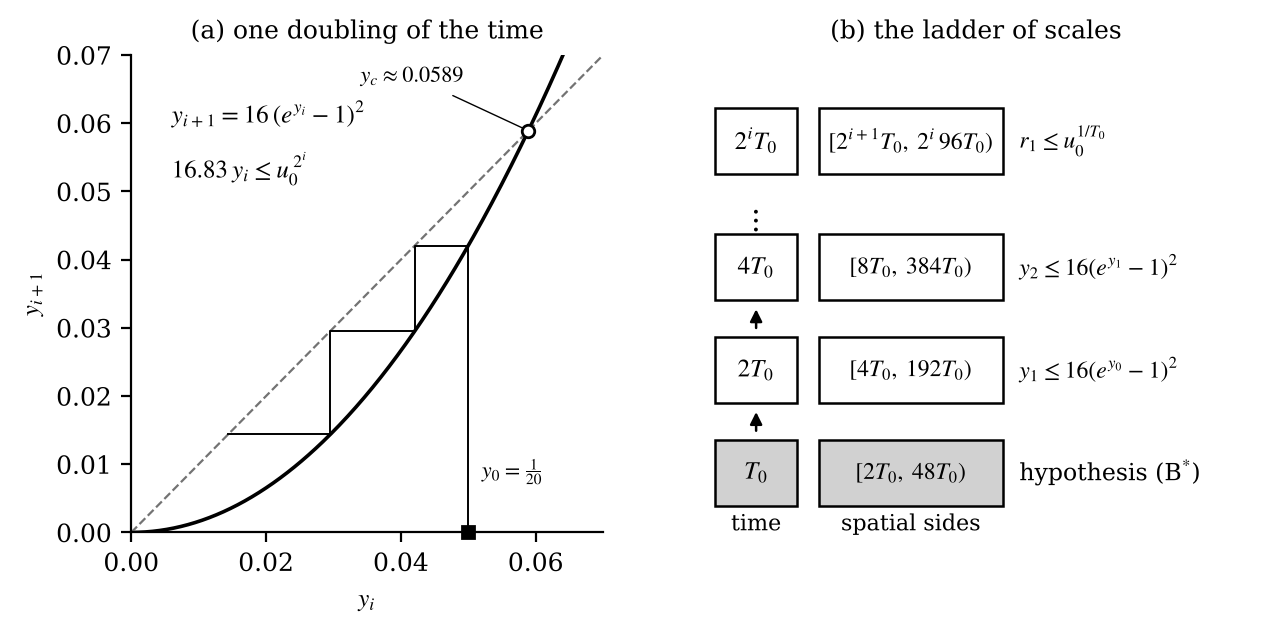
\includegraphics[width=\textwidth]{figures/fig_ascent.png}
\caption{The ascent of Theorem~\ref{thm:ascentfree}. (a) One doubling of the time extent maps the normalised pressure $y_i$ to at most $16(e^{y_i}-1)^2$; below the fixed point $y_c$ the iteration decreases doubly exponentially, and the starting value $y_0\le\frac1{20}$ lies below it. (b) The hypothesis is made at the single time extent $T_0$ (grey); every larger scale, with its gap, is a consequence.}
\label{fig:ascent}
\end{figure}

\begin{mainthmF}[the mass gap from one scale]\label{thm:F}
Let a continuum family satisfy \textup{(W)}, and suppose there are $t_0>0$,
$y_0\le\frac1{20}$ and $p_0$, $N_0(p)$ such that for all $p\ge p_0$ and $N\ge
N_0(p)$ there is an integer $T_0$ with $3\le T_0\le Nt_0$ for which
\textup{(B$^*$)} holds at the coupling $\beta_{N,p}$ with $\gamma=y_0/(2(96
T_0)^3)$. Put $u_0=16.83\,y_0$ and
\[
\Delta=\frac{\log(1/u_0)}{t_0}\ge\frac{0.172}{t_0} .
\]
Then, for $L_p\ge2t_0$:
\begin{enumerate}[label=\textup{(\roman*)},leftmargin=*]
\item $\mathcal Z_{N,p}-1\le1.9\cdot10^{-11}e^{-\Delta L_p/2}$, so the family
satisfies \textup{(Z)};
\item every eigenvalue $\lambda\ne\lambda_0$ of the transfer matrix of the
cylinder of spatial side $NL_p$ satisfies $0\le\lambda\le e^{-\Delta/N}
\lambda_0$;
\item the conclusion of Theorem~\ref{thm:E} holds with this $\Delta$: $S^\chi$
does not depend on $\chi$, and the Wightman theory of \textup{(W)} has
$\sigma(H)\subset\{0\}\cup[\Delta,\infty)$ with $0$ a simple eigenvalue.
\end{enumerate}
Neither \textup{(U)}, nor \textup{(D$_\ell$)}, nor the slab hypothesis
\textup{(M)}, nor \textup{(G$_{24}$)} is assumed.
\end{mainthmF}

\begin{proof}
Put $n=NL_p$; then $n\ge2Nt_0\ge2T_0$. (i) is
Theorem~\ref{thm:ascentfree}(c), with $u_0^{\,n/(2T_0)}\le u_0^{L_p/(2t_0)}=
e^{-\Delta L_p/2}$ because $T_0\le Nt_0$ and $u_0<1$; and $L_p\to\infty$.
(ii) is Theorem~\ref{thm:ascentfree}(b) for the cube of side $n$: $r_1\le
u_0^{1/T_0}\le u_0^{1/(Nt_0)}=e^{-\Delta/N}$, the eigenvalues being
nonnegative by Lemma~\ref{lem:transfer}(vii). (iii) In Step~1 of
Section~\ref{ssec:assembly}, hypothesis (D$_\ell$) enters only through
Proposition~\ref{prop:cylindergap}, which gives the transfer matrix of the
cylinder of side $NL_p$ a gap $m$ with $mN\ge\Delta$, and
Lemma~\ref{lem:gaptodecay} then gives~\eqref{eq:latticeineq} with the factor
$e^{-mN(\sigma-\sigma_1)}\le e^{-\Delta(\sigma-\sigma_1)}$. Here (ii) is that
gap, with $m=\Delta/N$, so~\eqref{eq:latticeineq} holds with the factor
$e^{-\Delta(\sigma-\sigma_1)}$. By (i) and Proposition~\ref{prop:ZgivesU},
\textup{(W)} gives \textup{(U$_w$)}, and the proof of
Corollary~\ref{cor:Z} derives~\eqref{eq:limitineq} from~\eqref{eq:latticeineq}
and \textup{(U$_w$)}, using the gap only through that factor. Steps~3
and~4 use~\eqref{eq:limitineq} and \textup{(W)} alone.
\end{proof}

Theorem~F replaces the hypotheses (D$_\ell$) or (M), (G$_{24}$), (Z) and (U)
by one bound at one scale. That bound does not involve the side $L_p$, an
insertion or a renormalisation constant, and it has a finite form.

\begin{proposition}[finite form]\label{prop:Bfinite}
With $\psi_s(T)=2\log Z(s,T)-\log Z(s,2T)$ as in Section~\ref{ssec:onescale},
hypothesis \textup{(B$^*$)} with the constant $\gamma$ follows from
\[
\textup{(B$^{**}$)}\qquad Z(s,T_0)^2\le e^{\gamma V(s)}\,Z(s,2T_0)\qquad
\text{for every }s\text{ with all its sides in }[2T_0,48T_0),
\]
and \textup{(B$^*$)} with $\gamma$ implies \textup{(B$^{**}$)} with $2\gamma$.
\textup{(B$^{**}$)} compares the partition functions of $2\cdot(46T_0)^3$
finite four-dimensional tori and is unchanged when $Z(n)$ is multiplied by
$e^{a|n|}$.
\end{proposition}

\begin{proof}
Lemma~\ref{lem:doubling} for the time transfer matrix of $s$ gives $\log
\mathcal Z_s(T_0)\le\psi_s(T_0)\le2\log\mathcal Z_s(T_0)$, and (B$^{**}$) is
$\psi_s(T_0)\le\gamma V(s)$.
\end{proof}

With $\rho=\mathbb R^{T_0}/\Tr\mathbb R^{T_0}$, the thermal state of the
torus $s$ at the time extent $T_0$, the ratio $Z(s,2T_0)/Z(s,T_0)^2$ is
$\Tr\rho^2$, so (B$^{**}$) says that this state is nearly pure: $\Tr\rho^2\ge
e^{-\gamma V(s)}$. In physical terms (B$^{**}$) asks that the thermal part of the free energy
at the temperature $1/t_0$, in boxes of sides between $2t_0$ and $48t_0$, be
at most $y_0/(2\cdot96^3t_0^3)\le2.9\cdot10^{-8}\,t_0^{-3}$ per unit volume.
Two results delimit what a proof of it must contain.

\begin{proposition}[\textup{(B$^*$)} contains the lattice mass gap]
\label{prop:Bhard}
Suppose \textup{(B$^*$)} holds at a coupling $\beta$ for some $T_0$, and let
$\mu^0_n$ be the zero-temperature state of the cylinder of spatial side $n$.
Then for every $n\ge2T_0$, every bounded measurable function $F$ of a slab
$[0,w]$ and every integer $s\ge0$,
\[
0\le\mu^0_n(\vartheta\bar F\,\tau_sF)-|\mu^0_n(F)|^2\le\|F\|_\infty^2\,
e^{-\delta_*s},\qquad\delta_*=\frac{\log(1/u_0)}{T_0},
\]
and the same bound holds, for local $F$, for every weak-$*$ limit point of
$(\mu^0_n)_n$ on $\Z^3\times\Z$.
\end{proposition}

\begin{proof}
By Lemma~\ref{lem:transfer}(v) the middle term is $\ip{\Psi'_F}{\mathbb R^s
\Psi'_F}$ with $\Psi'_F\perp\Omega_0$. By Theorem~\ref{thm:ascentfree}(b),
$0\le\mathbb R\le e^{-\delta_*}$ on $\Omega_0^\perp$, and $\|\Psi'_F\|^2\le
\|\Psi_F\|^2=\mu^0_n(\vartheta\bar F\,F)\le\|F\|_\infty^2$. The bound is
uniform in $n$, so it passes to limit points.
\end{proof}

A proof of (B$^*$) along couplings $\beta\to\infty$ therefore proves
exponential clustering of four-dimensional lattice Yang--Mills theory at
arbitrarily weak coupling, with a rate $\log(1/u_0)/T_0(\beta)$. The base
scale $T_0(\beta)$ cannot stay bounded, by the next theorem: at a fixed
lattice size the gap closes as $\beta\to\infty$. We state it for $\SU(2)$,
where the weight of Section~\ref{sec:lattice} is $\exp(c\sum_p\ReTr Q_p)$
with $c=2\beta$.

\begin{theorem}[the gap closes at a fixed lattice size]\label{thm:gapcloses}
Let $G=\SU(2)$, $c=2\beta\ge\frac1{32}$ and
\[
\varepsilon(c)=\frac{12(\log c+5.42)}{c} .
\]
For every spatial torus $t=(\ell_1,\ell_2,\ell_3)$ with sides at least $3$
and $(\ell_1\ell_2)^2\varepsilon(c)<3$,
\[
1-r_1(t)\le\frac{2(\ell_1+\ell_2)^2\,\varepsilon(c)}{1-(\ell_1\ell_2)^2
\varepsilon(c)/3} .
\]
\end{theorem}

\begin{proof}
Write $A_p=2-\Tr Q_p=\frac12\|Q_p-1\|_F^2\in[0,4]$, with the Frobenius norm,
since $\|U-1\|_F^2=4-2\Tr U$ for $U\in\SU(2)$.

\emph{Step 1: an energy bound uniform in the torus.} On a torus with $|n|$
sites, $4|n|$ links and $6|n|$ plaquettes let $A=\sum_pA_p$ and $\tilde Z(c)=
\int e^{-cA}\prod_edQ_e\le1$, so that the Wilson measure is $\tilde Z(c)^{-1}
e^{-cA}\prod_edQ_e$ and $\E_c[A]=-(\log\tilde Z)'(c)$. Since $(\log\tilde
Z)''=\Var_c(A)\ge0$, the mean $\E_c[A]$ is nonincreasing in $c$, and
\[
\frac c2\,\E_c[A]\le\int_{c/2}^c\E_{c'}[A]\,dc'=\log\tilde Z(c/2)-\log\tilde
Z(c)\le-\log\tilde Z(c).
\]
If every link has $\|Q_e-1\|_F\le r$, then $\|Q_p-1\|_F\le4r$ and $A_p\le8r^2$.
In the class angle $\theta\in[0,\pi]$, with $\Tr U=2\cos\theta$, Haar
measure is $\frac2\pi\sin^2\theta\,d\theta$ and $\|U-1\|_F=\sqrt8\sin(\theta/
2)$. The ball of radius $r\le2$ is $\{\theta\le\theta_r\}$ with $\theta_r=2
\arcsin(r/\sqrt8)\in[r/\sqrt2,\pi/2]$, and by $\sin\theta\ge2\theta/\pi$ on
$[0,\pi/2]$ its measure is at least $\frac2\pi\int_0^{\theta_r}(2\theta/\pi)^2
d\theta=8\theta_r^3/(3\pi^3)\ge2\sqrt2\,r^3/(3\pi^3)\ge r^3/33$. With $r^2=1/
(8c)$, which has $r\le2$ because $c\ge\frac1{32}$, restricting the integral
to these balls gives $\tilde Z(c)\ge e^{-6|n|}(r^3/33)^{4|n|}$, so
\[
\E_c[A]\le\frac2c\,|n|\bigl(6+4\log33+6\log(8c)\bigr)\le\frac{12}c\,|n|\,
(\log c+5.42).
\]
The $|n|$ translates of a plaquette have equal expectation and $A_p\ge0$,
so $\E_c[A_p]\le\varepsilon(c)$ for every plaquette on every torus, and by
Lemma~\ref{lem:transfer}(v) the same bound holds for $\mu^0_t=\lim_M\mu_{t,M}$.

\emph{Step 2: three slice functions of mean zero.} On the slice at time $0$
let $P_1$ and $P_2$ be the ordered products of the links from the origin
once around the directions $1$ and $2$, and $F_1=\Tr P_1$, $F_2=\Tr P_2$,
$F_3=\Tr(P_1P_2)$; they are real, continuous and gauge invariant, being
traces of closed loops. The centre flip $z_1$, which replaces $Q_{(x,1)}$ by
$-Q_{(x,1)}$ on all links in the direction $1$ with $x_1=0$, at all times,
preserves Haar measure and every plaquette variable, because the two links
in the direction $1$ of a plaquette have the same coordinate $x_1$, so a
plaquette contains none or two of the flipped links. It therefore preserves
$\mu_{t,M}$ and $\mu^0_t$, and it maps $F_1$ to $-F_1$ and $F_3$ to $-F_3$.
The flip $z_2$ maps $F_2$ to $-F_2$. So $\mu^0_t(F_k)=0$ for $k=1,2,3$, that
is, $F_k\Omega_0\perp\Omega_0$.

\emph{Step 3: the three functions are not all small.} For $A,B\in\SU(2)$
with $x=\Tr A$, $y=\Tr B$ and $z=\Tr AB$, Fricke's identity is
\[
\Tr(ABA^{-1}B^{-1})=x^2+y^2+z^2-xyz-2 ;
\]
it follows from $\Tr(AB)+\Tr(AB^{-1})=xy$, applied three times.\footnote{The
Cayley--Hamilton identity $B+B^{-1}=y\cdot1$ gives $\Tr(AB)+\Tr(AB^{-1})=xy$
for $A,B\in\SU(2)$. Hence $\Tr(ABA^{-1}B^{-1})=\Tr(AB)\Tr(A^{-1}B^{-1})-
\Tr(ABBA)$, $\Tr(A^{-1}B^{-1})=\Tr(BA)=z$, and $\Tr(ABBA)=\Tr(A^2B^2)=\Tr(A^2B)
y-\Tr(A^2)$, with $\Tr(A^2B)=xz-y$ and $\Tr(A^2)=x^2-2$; so the commutator has
trace $z^2-(xz-y)y+x^2-2$.} Put $\sigma=x^2+y^2+z^2$ and $\eta=2-\Tr(ABA^{-1}
B^{-1})\ge0$. Since $|xyz|\le(\sigma/3)^{3/2}$, the function $\phi(\sigma)=
\sigma+(\sigma/3)^{3/2}$ satisfies $\phi(\sigma)\ge4-\eta$. As $\phi(3)=4$ and
$\phi'\ge1$, $\sigma<3$ gives $3-\sigma\le\phi(3)-\phi(\sigma)\le\eta$; so
$\sigma\ge3-\eta$ in every case. Apply this to $A=P_1$ and $B=P_2$. The
commutator $K=P_1P_2P_1^{-1}P_2^{-1}$ is the holonomy of the boundary of the
sheet of the $\ell_1\ell_2$ plaquettes of the $(1,2)$-plane through the
origin, cut open along the two cycles. Adding the plaquettes of the sheet
one at a time, row by row, so that each step keeps a disc, multiplies the
boundary holonomy by a conjugate of $Q_p^{\pm1}$; so $K$ is a product of
$\ell_1\ell_2$ conjugates of the $Q_p^{\pm1}$, and $\|UV-1\|_F\le\|U-1\|_F+
\|V-1\|_F$ for unitary matrices gives $\|K-1\|_F\le\sum_p\|Q_p-1\|_F$.
Hence, by the Cauchy--Schwarz inequality,
\[
\eta=\tfrac12\|K-1\|_F^2\le\tfrac12\Bigl(\sum_p\sqrt{2A_p}\Bigr)^2\le\ell_1
\ell_2\sum_{p}A_p,\qquad\mu^0_t(\eta)\le(\ell_1\ell_2)^2\varepsilon ,
\]
the sums over the plaquettes of the sheet. So $\sum_k\mu^0_t(F_k^2)\ge3-(\ell_1
\ell_2)^2\varepsilon$, and some $k$ has $\|F_k\Omega_0\|^2=\mu^0_t(F_k^2)\ge1-
(\ell_1\ell_2)^2\varepsilon/3$.

\emph{Step 4: the Dirichlet form.} For a real function $F$ of the slice,
Lemma~\ref{lem:transfer}(v) with $w=w'=0$ and $s=1$, and the invariance of
$\mu^0_t$ under time translations, give
\[
\ip{F\Omega_0}{(1-\mathbb R)F\Omega_0}=\mu^0_t(F^2)-\mu^0_t(F\,\tau_1F)=\tfrac
12\,\mu^0_t\bigl((F-\tau_1F)^2\bigr).
\]
The loop of $F_k$ at time $0$ and its translate at time $1$, joined by the
temporal link at the origin, bound a strip of $m_k$ temporal plaquettes,
with $m_1=\ell_1$, $m_2=\ell_2$ and $m_3=\ell_1+\ell_2$. As in Step~3 the two
holonomies $X$ and $Y$, the second conjugated by the temporal link, satisfy
$\|X-Y\|_F\le\sum_p\|Q_p-1\|_F$ over the strip, and $|\Tr X-\Tr Y|\le\sqrt2\,
\|X-Y\|_F$. So $(F_k-\tau_1F_k)^2\le4m_k\sum_pA_p$ and
\[
\tfrac12\,\mu^0_t\bigl((F_k-\tau_1F_k)^2\bigr)\le2m_k^2\,\varepsilon\le2(\ell_1+
\ell_2)^2\varepsilon .
\]

\emph{Step 5.} On $\Omega_0^\perp$ one has $\mathbb R\le r_1$, so for the $k$
of Step~3, $1-r_1\le\ip{F_k\Omega_0}{(1-\mathbb R)F_k\Omega_0}/\|F_k\Omega_0\|^2$,
which is the claim.
\end{proof}

\begin{corollary}[the base scale diverges]\label{cor:basescale}
If \textup{(B$^*$)} holds for $\SU(2)$ with the base scale $T_0$ at a
coupling with $\varepsilon=\varepsilon(2\beta)\le10^{-3}$, then
\[
T_0>\Bigl(\frac3{32\,\varepsilon}\Bigr)^{1/4}=\Bigl(\frac{\beta}{64(\log2\beta
+5.42)}\Bigr)^{1/4}.
\]
\end{corollary}

\begin{proof}
On the cube $t$ of side $2T_0$, (B$^*$) gives $r_1^{T_0}\le D_t(T_0)\le e^{8
\gamma T_0^3}-1=e^{4y_0/96^3}-1\le2.3\cdot10^{-7}$, so $r_1\le e^{-x}$ with $x=
15.28/T_0$, and by concavity $1-r_1\ge(1-e^{-1})\min\{1,x\}\ge\min\{0.632,\,
9.6/T_0\}$. Suppose $T_0^4\varepsilon\le\frac3{32}$. Then $(2T_0)^4\varepsilon
\le\frac32$, and Theorem~\ref{thm:gapcloses} with $\ell_1=\ell_2=2T_0$ gives
$1-r_1\le64T_0^2\varepsilon$. If $T_0\le15$ this is at most $64\sqrt{3/32}\,
\sqrt\varepsilon\le0.62<0.632$, and if $T_0\ge16$ it gives $T_0^3\varepsilon
\ge0.15$, while $T_0^3\varepsilon\le\frac3{32\cdot16}<0.006$. Both are
impossible.
\end{proof}

Thus no tuning with $\beta_N\to\infty$ has its base scale at a bounded
number of lattice units, and a bound of the shape of
Proposition~\ref{prop:Zstrongsharp}, with a rate fixed in lattice units,
cannot serve along it (Proposition~\ref{prop:nofixedrate}); the mechanism
is the centre symmetry, which gives the Polyakov loops mean zero while the
action no longer suppresses their fluctuation at a fixed lattice size. The
proof of Theorem~\ref{thm:ascentfree} uses of the Wilson action only that
$Z$ is symmetric in the four sides and is, in each direction, the trace of
a power of a nonnegative self-adjoint Hilbert--Schmidt operator with a
simple largest eigenvalue.
What remains open for four-dimensional Yang--Mills theory at weak coupling
is therefore (W) and the one bound \textup{(B$^{**}$)}, for integers $T_0
(\beta)\to\infty$ along a sequence $\beta\to\infty$:
\[
Z(s,T_0)^2\le\exp\Bigl(\frac{V(s)}{40\,(96T_0)^3}\Bigr)Z(s,2T_0)\qquad
\text{for every }s\text{ with all its sides in }[2T_0,48T_0).
\]
Neither is proved here.

\section{Positive torus systems and a single-cube datum}\label{sc:sec:psts}

The one-scale criterion of Theorem~\ref{thm:F} asks for a window of box shapes.
We now replace that window by one cube and improve the physical gap constant.
Every argument in this section and the next is a theorem about positive transfer
operators and permutation symmetry. These properties do not supply the
weak-coupling datum; their role is to propagate it once it has been proved.
The new notation is local to these sections: $N_c$ is the dimension of a faithful
unitary representation, while $N=1/a_N$ is the inverse lattice spacing.

\subsection{The positive torus system}
For $n=(n_1,n_2,n_3,n_4)\in\Z^4$ with all $n_\mu\ge3$ let $\Lambda(n)=\prod_{\mu=1}^4\Z/n_\mu\Z$ and $|n|=n_1n_2n_3n_4$. A \emph{spatial torus} is a triple $s=(s_1,s_2,s_3)$ of integers $s_j\ge3$, with volume $\Vol{s}=s_1s_2s_3$. We write $(s,M)$ for $(s_1,s_2,s_3,M)$ and call its last entry time; $L^3$ stands for $(L,L,L)$ and $L^4$ for $(L^3,L)$, so that $\cube{T}$ is the spatial cube of side $2T$.

A \emph{positive symmetric torus system} (\PSTS) is a function $n\mapsto Z(n)$ on $\{n\in\Z^4:n_\mu\ge3\}$ with the following two properties.
\begin{enumerate}[label=(P\arabic*),leftmargin=3em]
\item $Z(n)\ge1$, and $Z(\pi n)=Z(n)$ for every permutation $\pi$ of the four entries of $n$.
\item For every spatial torus $s$ there is a nonzero self-adjoint Hilbert--Schmidt operator $\TT_s\ge0$ on a separable Hilbert space $\Kspace_s$ such that $\Zpart{s}{M}=\Tr\TT_s^M$ for all $M\ge3$.
\end{enumerate}
The system is \emph{simple} if the largest eigenvalue of every $\TT_s$ is simple. Simplicity is not part of the definition. The proofs below use the eigenvalue list with multiplicity; Theorem~\ref{sc:thm:ascent} subsequently proves simplicity on the large cubes covered by the datum.

Let $\lzero(s)=\norm{\TT_s}>0$; it is an eigenvalue of finite multiplicity, and $E_0(s)=-\log\lzero(s)$. The operator $R_s=\TT_s/\lzero(s)$ has eigenvalues $1=r_0(s)\ge r_1(s)\ge r_2(s)\ge\dots\ge0$, listed with multiplicity, and $\sum_ir_i(s)^2<\infty$. If there is only one nonzero eigenvalue, append zeros to the eigenvalue list. We use $-\log0=+\infty$, so a rank-one transfer operator has no finite-energy excited state. Thus $r_1(s)=1$ exactly when $\lzero(s)$ is degenerate, and $-\log r_1(s)$ is the spectral gap of $\TT_s$ in lattice units. For $T\ge2$ the operator $R_s^T$ is trace class, and we set
\begin{equation}\label{sc:eq:normalised}
\Zs{s}{T}=\Tr R_s^T=\sum_{i\ge0}r_i(s)^T,\qquad \XT{s}{T}=\log\Zs{s}{T},\qquad \Dexc{s}{T}=\Zs{s}{T}-1 .
\end{equation}
For $T\ge3$ one has $\Zs{s}{T}=\Zpart{s}{T}/\lzero(s)^T$, and the purity defect is
\begin{equation}\label{sc:eq:psi-def}
\psiT{s}{T}=2\log\Zpart{s}{T}-\log\Zpart{s}{2T}=2\XT{s}{T}-\XT{s}{2T}.
\end{equation}
Multiplying $Z(n)$ by $e^{a|n|}$, $a\in\R$, replaces $\TT_s$ by $e^{a\Vol{s}}\TT_s$ and changes neither $R_s$ nor any of the quantities in \eqref{sc:eq:normalised} and \eqref{sc:eq:psi-def}.

\smallskip
\noindent\emph{The datum.} Let $\Tzero\ge3$ be an integer. The system satisfies \Mcirc{} at $\Tzero$ if
\begin{equation}\label{sc:eq:datum-M}
\psiT{\cube{T_0}}{T_0}\le\dconst,\qquad\text{equivalently}\qquad \Zpart{\cube{T_0}}{T_0}^2\le e^{\dconstinl}\,Z\bigl((2T_0)^4\bigr),
\end{equation}
and it satisfies \Bcirc{} at $\Tzero$ if
\begin{equation}\label{sc:eq:datum-B}
\XT{\cube{T_0}}{T_0}\le\xconst .
\end{equation}
By \cref{sc:lem:purity-conversion}, \Mcirc{} at $T_0$ implies \Bcirc{} at $T_0$, which in turn implies $\psiT{\cube{T_0}}{T_0}\le1/4096$. For the continuum family of Definition~\ref{def:family} we say that \Mcirc{} holds \emph{along the tuning} with $\tzero>0$ if for every sufficiently large $p$ there is $N_0(p)$ such that for every $N\ge N_0(p)$ of the family the Wilson system at coupling $\betaNp$ satisfies \Mcirc{} at some integer $\Tzero$ with $3\le\Tzero\le N\tzero$; the same convention is used for \Bcirc{}. The strong-coupling and two-dimensional results retained above do not establish this datum along a four-dimensional weak-coupling tuning.

\subsection{Wilson systems and the scope in the gauge group}
\begin{proposition}[Wilson positivity]\label{sc:prop:wilson}
For every closed subgroup $G\subset\U(N_c)$ and $\beta\ge0$, the Wilson
partition functions with weight
$\exp(N_c\beta\sum_p\ReTr Q_p)$ form a simple positive symmetric torus system.
The criterion therefore applies to each compact simple gauge group whenever
its single-cube datum holds; it does not assert that datum for any group.
\end{proposition}
\begin{proof}
Use the transfer kernel of Lemma~\ref{lem:transfer} on a spatial torus $s$.
Its proof uses only compactness, Haar measure and the faithful unitary
representation; the argument does not use simplicity or connectedness of $G$.
For clarity, positivity follows from $\mathbb T_s=D\Pi K\Pi D$, where $D$ is
multiplication by the positive square root of the spatial weight, $\Pi$ is
Haar averaging over gauge transformations, and
$K(Q,Q')=\exp(N_c\beta\sum_e\ReTr(Q_eQ_e'^*))$. Identify matrix entries with
real coordinates. Expanding the exponential makes $K$ a uniformly convergent
nonnegative sum of tensor inner-product kernels, hence $K\ge0$ and
$\mathbb T_s\ge0$. The transfer kernel is continuous, symmetric and strictly
positive on the compact configuration space. It is Hilbert--Schmidt and its
top eigenvalue is simple by the positivity argument in
Lemma~\ref{lem:transfer}. Splitting the spatial plaquette action equally
between adjacent slices and integrating the temporal links gives
$Z(s,M)=\operatorname{Tr}\mathbb T_s^M$. Permuting the four lattice directions
preserves Haar measure and the real plaquette trace, so $Z$ is symmetric.
Finally Jensen's inequality gives $Z(n)\ge1$: each plaquette is Haar distributed
under the product Haar law, and $\int_G g\,dg$ is the orthogonal projection
onto invariant vectors, whose real trace is nonnegative. This proves (P1)
and (P2), including simplicity.
\end{proof}

The conclusion is conditional even for a connected simply connected group.
For a quotient group, or a theory with extra flux sectors, the entire thermal
trace must satisfy the datum; it is insufficient to check only one selected
sector. Thus the generality of the transfer argument is not a proof of its
weak-coupling hypothesis for every compact simple group.

\subsection{Trace inequalities}
\begin{lemma}[elementary trace bounds]\label{sc:lem:E1-E3}
Let $Z$ be a \PSTS{} and $s$ a spatial torus.
\begin{enumerate}[label=(E\arabic*),leftmargin=3em]
\item $\lzero(s)=\lim_{M\to\infty}\Zpart{s}{M}^{1/M}\ge1$, so $E_0(s)\le0$; $\lzero(s)$ and $\Zs{s}{M}$, $M\ge3$, are invariant under permutations of $s_1,s_2,s_3$.
\item $1\le\Zs{s}{M}\le\Zs{s}{2}<\infty$, and $M\mapsto\Zs{s}{M}$ is nonincreasing on $M\ge2$. For $M',M''\ge2$, $\Dexc{s}{M'+M''}\le\Dexc{s}{M'}\Dexc{s}{M''}$. If $r_1(s)\le e^{-\delta}$ with $\delta\ge0$, then $\Dexc{s}{M}\le e^{-\delta(M-M')}\Dexc{s}{M'}$ for $M\ge M'\ge2$.
\item For $T\ge3$ let $p_i=r_i(s)^T/\Zs{s}{T}$. Then $e^{-\psiT{s}{T}}=\sum_ip_i^2$, $p_0\ge p_i$ for all $i$, and
\begin{equation}\label{sc:eq:X-psi}
\XT{s}{T}\le\psiT{s}{T}\le2\,\XT{s}{T}.
\end{equation}
The constants $1$ and $2$ cannot be improved.
\end{enumerate}
\end{lemma}

\begin{proof}
(E1) By (P2), $\Zpart{s}{M}=\sum_i\lambda_i^M$ over the eigenvalues $\lambda_i\ge0$ of $\TT_s$, with multiplicity. For $M\ge3$, $\lzero^M\le\Zpart{s}{M}\le\lzero^{M-2}\sum_i\lambda_i^2$, so $\Zpart{s}{M}^{1/M}\to\lzero(s)$, and $\lzero(s)\ge1$ because $Z\ge1$. By (P1), $\Zpart{s}{M}$ is invariant under permutations of $s$ at fixed $M$, hence so are $\lzero(s)$ and $\Zs{s}{M}=\Zpart{s}{M}/\lzero(s)^M$.

(E2) $\Zs{s}{M}=\sum_ir_i^M$ with $r_0=1$ and $0\le r_i\le1$ gives the first two claims. Next, $\Dexc{s}{M'+M''}=\sum_{i\ge1}r_i^{M'}r_i^{M''}\le\sum_{i\ge1}r_i^{M'}\sum_{k\ge1}r_k^{M''}$, the omitted cross terms being nonnegative. If $r_i\le e^{-\delta}$ for $i\ge1$, then $\Dexc{s}{M}=\sum_{i\ge1}r_i^{M'}r_i^{M-M'}\le e^{-\delta(M-M')}\Dexc{s}{M'}$.

(E3) By \eqref{sc:eq:psi-def}, $e^{-\psiT{s}{T}}=\Zs{s}{2T}/\Zs{s}{T}^2=\sum_ip_i^2$, and $p_0=1/\Zs{s}{T}\ge p_i$ since $r_i\le1$. Hence $p_0^2\le\sum_ip_i^2\le p_0\sum_ip_i=p_0=e^{-\XT{s}{T}}$, which is \eqref{sc:eq:X-psi}. For sharpness take $Z(n)=1+q\rho^{|n|}$ with an integer $q\ge1$ and $0<\rho<1$. It is a \PSTS{} with $\TT_s=\mathrm{diag}(1,\rho^{\Vol{s}},\dots,\rho^{\Vol{s}})$ on $\C^{1+q}$. With $a=\rho^{\Vol{s}T}$ one has $\XT{s}{T}=\log(1+qa)$ and $\psiT{s}{T}=2\log(1+qa)-\log(1+qa^2)$. As $\rho\uparrow1$ at fixed $q$ both tend to $\log(1+q)$, so $\psi/X\to1$; as $\rho\downarrow0$ with $q=1$, $\psi/X\to2$.
\end{proof}
\subsection{Exchange of directions and elongation}

Permutation symmetry lets one read the same torus with a spatial direction as time. For fixed transverse sides this turns the thermal trace of a long box into that of a short box, at the price of a free energy per unit length. The exchange identity follows directly from the two readings of the same partition function.

\begin{lemma}[exchange of directions]\label{sc:lem:exchange}
Let $Z$ be a \PSTS{}, fix integers $b,c\ge3$, and put $g(\ell)=\log\lzero(\ell,b,c)$ for $\ell\ge3$.
\begin{enumerate}[label=(\alph*)]
\item The limit $\bar e=\lim_{M\to\infty}g(M)/M$ exists and equals $\inf_{\ell\ge3}g(\ell)/\ell\in[0,g(3)/3]$. The function $\zeta(\ell)=g(\ell)-\ell\bar e$ satisfies $\zeta(\ell)=\lim_{M\to\infty}M^{-1}\log\Zs{(M,b,c)}{\ell}$, and it is nonnegative and nonincreasing on $\ell\ge3$.
\item For all integers $m,T\ge3$,
\begin{equation}\label{sc:eq:exchange}
\log\Zs{(m,b,c)}{T}=m\,\zeta(T)-T\,\zeta(m)+\log\Zs{(T,b,c)}{m}.
\end{equation}
\item For every integer $T\ge3$, $\log\Zs{(2T,b,c)}{T}=\log\Zs{(T,b,c)}{2T}+T\delta_T$ with $\delta_T=2\zeta(T)-\zeta(2T)\in[\zeta(T),2\zeta(T)]$.
\end{enumerate}
By (E1) the same holds with the varying side in any of the three spatial positions.
\end{lemma}

\begin{proof}
By (P1), $Z((\ell,b,c),M)=Z((M,b,c),\ell)$ for $\ell,M\ge3$, that is,
\begin{equation}\label{sc:eq:exchange-basic}
M\,g(\ell)+\log\Zs{(\ell,b,c)}{M}=\ell\,g(M)+\log\Zs{(M,b,c)}{\ell}.
\end{equation}
Divide by $\ell M$. Since $\log\Zs{(M,b,c)}{\ell}\ge0$ and $0\le\log\Zs{(\ell,b,c)}{M}\le\log\Zs{(\ell,b,c)}{2}<\infty$ by (E2), $g(M)/M\le g(\ell)/\ell+\log\Zs{(\ell,b,c)}{2}/(\ell M)$. Hence $\limsup_Mg(M)/M\le\inf_\ell g(\ell)/\ell\le\liminf_Mg(M)/M$, which gives $\bar e$ and the formula for it; $\bar e\ge0$ because $g\ge0$ by (E1). Dividing \eqref{sc:eq:exchange-basic} by $M$ and letting $M\to\infty$ gives $g(\ell)=\ell\bar e+\lim_MM^{-1}\log\Zs{(M,b,c)}{\ell}$, the formula for $\zeta$. Then $\zeta\ge0$ since $\Zs{(M,b,c)}{\ell}\ge1$, and $\zeta$ is nonincreasing because $\ell\mapsto\Zs{(M,b,c)}{\ell}$ is, by (E2). Substituting $g(\ell)=\zeta(\ell)+\ell\bar e$ and $g(M)=\zeta(M)+M\bar e$ in \eqref{sc:eq:exchange-basic}, the terms $\ell M\bar e$ cancel, and renaming $(M,\ell)$ as $(m,T)$ gives \eqref{sc:eq:exchange}. Part (c) is \eqref{sc:eq:exchange} at $m=2T$, and $\zeta(T)\le\delta_T\le2\zeta(T)$ follows from $0\le\zeta(2T)\le\zeta(T)$.
\end{proof}

Since $\zeta(m)\ge0$ and the last term of \eqref{sc:eq:exchange} does not increase with $m$, one side of a box can be made long at a cost proportional to its length.

\begin{lemma}[elongation]\label{sc:lem:elongation}
Let $Z$ be a \PSTS{}, $b,c\ge3$, and let $m\ge m_0>T\ge3$ be integers. Put $L_0=\log\Zs{(m_0,b,c)}{T}$ and $Y_0=\log\Zs{(T,b,c)}{m_0}$. Then $0\le Y_0\le L_0$, $(m_0-T)\,\zeta(T)\le L_0-Y_0$, and
\begin{equation}\label{sc:eq:elongation}
\log\Zs{(m,b,c)}{T}\le\frac{m}{m_0-T}\,(L_0-Y_0)+Y_0\le\frac{m}{m_0-T}\,\log\Zs{(m_0,b,c)}{T}.
\end{equation}
Consequently $\psiT{(m,b,c)}{T}\le\frac{2m}{m_0-T}\,\psiT{(m_0,b,c)}{T}$.
\end{lemma}

\begin{proof}
By \eqref{sc:eq:exchange} at $m_0$, $L_0-Y_0=m_0\zeta(T)-T\zeta(m_0)\ge(m_0-T)\zeta(T)\ge0$, because $0\le\zeta(m_0)\le\zeta(T)$; and $Y_0\ge0$ by (E2). By \eqref{sc:eq:exchange} at $m$, with $\zeta(m)\ge0$ and $\Zs{(T,b,c)}{m}\le\Zs{(T,b,c)}{m_0}$ from (E2),
\[
\log\Zs{(m,b,c)}{T}\le m\,\zeta(T)+Y_0\le\frac{m}{m_0-T}(L_0-Y_0)+Y_0 .
\]
As $m/(m_0-T)\ge1$, the right-hand side is at most $\frac{m}{m_0-T}L_0$. The last claim follows from \eqref{sc:eq:X-psi}: $\psiT{(m,b,c)}{T}\le2\log\Zs{(m,b,c)}{T}\le\frac{2m}{m_0-T}L_0\le\frac{2m}{m_0-T}\psiT{(m_0,b,c)}{T}$.
\end{proof}


\subsection{From purity to thermal pressure}
\begin{lemma}[purity conversion]\label{sc:lem:purity-conversion}
Let $Z$ be a \PSTS{}, $s$ a spatial torus, $T\ge3$ and $0<x\le1/8$. If $\psiT{s}{T}\le2x-3x^2$, then $\XT{s}{T}\le x$. In particular \Mcirc{} at $T_0$ implies \Bcirc{} at $T_0$, and \Bcirc{} at $T_0$ implies $\psiT{\cube{T_0}}{T_0}\le1/4096$.
\end{lemma}

\begin{proof}
Let $P=e^{-\psiT{s}{T}}=\sum_ip_i^2$ and $q=p_0=e^{-\XT{s}{T}}$, with $p_i$ as in (E3). Then $P\le q$ by (E3), and $P\le q^2+\bigl(\sum_{i\ge1}p_i\bigr)^2=h(q)$ with $h(y)=y^2+(1-y)^2$. Since $\psiT{s}{T}\le2x\le1/4$, $q\ge P\ge1-\psiT{s}{T}\ge3/4$. Suppose $\XT{s}{T}>x$, that is, $q<e^{-x}$. Now $e^{-x}\le q_U=1-x+\frac12x^2\le1$ and $h$ is strictly increasing on $[\frac12,1]$, so
\[
P\le h(q)<h(q_U)=1-2x+3x^2-2x^3+\tfrac12x^4\le1-2x+3x^2 .
\]
On the other hand $P=e^{-\psiT{s}{T}}\ge1-\psiT{s}{T}\ge1-2x+3x^2$, a contradiction. For $x=\xconstinl$, $2x-3x^2=16381/2^{26}$, and $\dconstinl\le16381/2^{26}$ because $16381\cdot4097=67\,112\,957\ge2^{26}=67\,108\,864$. So \Mcirc{} at $T_0$ implies \Bcirc{} at $T_0$.\footnote{The converse fails at the same $T_0$. For the \PSTS{} $Z(n)=1+\rho^{|n|}$ with $\rho^{8T_0^4}=a=e^{\xconstinl}-1$ one has $\XT{\cube{T_0}}{T_0}=\xconstinl$ and $\psiT{\cube{T_0}}{T_0}=1/4096-\log(1+a^2)>\dconstinl$, since $a=e^{1/8192}-1<1/8191$ (from $e^y-1\le y/(1-y)$ for $0\le y<1$), so $\log(1+a^2)\le a^2<1/8191^2<1/(4096\cdot4097)$.} The last claim is \eqref{sc:eq:X-psi}.
\end{proof}
\section{A single cube controls all larger scales}\label{sc:sec:ascent}
Throughout this section $Z$ is a positive symmetric torus system; simplicity
of its largest eigenvalue is not assumed. Write
$X(T)=\XT{\cube T}{T}$ for $T\ge3$. The trace bounds give
\begin{equation}\label{sc:eq:gap-step}
\Dexc{s}{M'+M''}\le\Dexc{s}{M'}\Dexc{s}{M''},\qquad
\Dexc{s}{M}\le r_1(s)^{M-M'}\Dexc{s}{M'}\quad(M\ge M'\ge2).
\end{equation}
Indeed $\Dexc{s}{M}=\sum_{i\ge1}r_i^{M}$ and $0\le r_i\le r_1\le1$.
Also $r_1(s)^T\le\Dexc{s}{T}$ and
$\XT{s}{T}=\log(1+\Dexc{s}{T})\le\Dexc{s}{T}$.

\subsection{The comparison of boxes}
\begin{theorem}[one box controls all larger boxes]\label{sc:thm:cube-control}
Let $T\ge3$, and let $a=(a_1,a_2,a_3)$ and $t=(t_1,t_2,t_3)$ be spatial tori with $t_j\ge a_j>T$ for $j=1,2,3$. Then
\begin{equation}\label{sc:eq:box-control}
\log\Zs{t}{T}\le\prod_{j=1}^3\frac{t_j}{a_j-T}\cdot\log\Zs{a}{T}.
\end{equation}
In particular every spatial torus $t$ with all sides at least $2T$ satisfies
\begin{equation}\label{sc:eq:cube-control}
\log\Zs{t}{T}\le\frac{\Vol{t}}{T^3}\,X(T).
\end{equation}
\end{theorem}

\begin{proof}
By \cref{sc:lem:elongation} with $(m,m_0,b,c)=(t_1,a_1,t_2,t_3)$, $\log\Zs{(t_1,t_2,t_3)}{T}\le\frac{t_1}{a_1-T}\log\Zs{(a_1,t_2,t_3)}{T}$. By (E1), $\Zs{(a_1,t_2,t_3)}{T}=\Zs{(t_2,a_1,t_3)}{T}$, and the lemma with $(m,m_0,b,c)=(t_2,a_2,a_1,t_3)$ gives the factor $t_2/(a_2-T)$ and the box $(a_2,a_1,t_3)$. A third application, with $(m,m_0,b,c)=(t_3,a_3,a_1,a_2)$ after a permutation, gives the factor $t_3/(a_3-T)$ and a permutation of $a$. All sides that occur are at least $T+1\ge4$, all factors are at least $1$ and all logarithms are nonnegative, so the three bounds compose to \eqref{sc:eq:box-control}. For $a=(2T,2T,2T)$ the product is $\prod_jt_j/T=\Vol{t}/T^3$.
\end{proof}
\subsection{The ascent and the improved gap constant}
Put $f(x)=(e^{64x}-1)^2$, $u=32/63$ and $\theta=127/126$.
The proof below derives a superexponentially decreasing envelope from one
small datum; it does not estimate the value of that datum at weak coupling.
\begin{theorem}[ascent from one cube]\label{sc:thm:ascent}
Let $T_0\ge3$, $T_i=2^iT_0$, and suppose \Bcirc{} at $T_0$, that is $X(T_0)\le\xconstinl$. Put $x_0=\xconstinl$, $x_{i+1}=f(x_i)$ and $v_i=e^{64x_i}-1$. Then the following hold.
\begin{enumerate}[label=(\alph*)]
\item $X(T_i)\le x_i$ and $v_i\le u^{2^i}/64$ for every $i\ge0$, and every spatial torus $t$ with all sides at least $2T_i$ satisfies $\log\Zs{t}{T_i}\le x_i\Vol{t}/T_i^3$.
\item If all sides of $t$ lie in $[2T_i,4T_i)$ for some $i\ge0$, in particular if $t=n^3$ with $n\ge2T_0$, then $r_1(t)\le u^{1/T_0}$. So $\lzero(t)$ is simple and the spectral gap $-\log r_1(t)$ is at least $T_0^{-1}\log\frac{63}{32}>0.677/T_0$.
\item Every cube of side $n\ge2T_0$ satisfies $\Zs{n^3}{n}-1\le u^{n/(2T_0)}/4096$.
\end{enumerate}
Moreover \Bcirc{} at $T_0$ follows from \Mcirc{} at $T_0$, that is from $\Zpart{\cube{T_0}}{T_0}^2\le e^{\dconstinl}\Zpart{\cube{T_0}}{2T_0}$.
\end{theorem}

\begin{proof}
(a) We prove $X(T_i)\le x_i$ by induction on $i$; given it, the last claim of (a) is \eqref{sc:eq:cube-control} at $T=T_i$. The case $i=0$ is \Bcirc{}. Let $s=(4T_i,4T_i,4T_i)=\cube{T_{i+1}}$. Its sides are at least $2T_i$ and $\Vol{s}/T_i^3=64$, so $\log\Zs{s}{T_i}\le64x_i$ and $\Dexc{s}{T_i}\le e^{64x_i}-1=v_i$. By \eqref{sc:eq:gap-step},
\[
X(T_{i+1})=\log\Zs{s}{2T_i}\le\Dexc{s}{2T_i}\le\Dexc{s}{T_i}^2\le v_i^2=x_{i+1}.
\]
For the numbers we show $v_i\le\theta^{-1}u^{2^i}/64$, which is stronger than the claim. We use $e^y-1\le y/(1-y)$ for $0\le y<1$. For $i=0$, $v_0=e^{1/128}-1\le1/127=\theta^{-1}u/64$. Suppose $v_i\le\theta^{-1}u^{2^i}/64$; then $v_i\le1/127$, and $y=64x_{i+1}=64v_i^2\le64/16\,129<1/252$, because $64\cdot252=16\,128$. Hence
\[
v_{i+1}=e^y-1\le\frac{252}{251}\,y\le\theta\cdot64v_i^2\le\theta\cdot64\,\theta^{-2}\frac{u^{2^{i+1}}}{4096}=\theta^{-1}\frac{u^{2^{i+1}}}{64},
\]
using $252/251\le127/126$, that is $252\cdot126=31\,752\le31\,877=251\cdot127$.

(b) Since every side of $t$ is less than $4T_i$, $\Vol{t}<64T_i^3$, and (a) gives $\log\Zs{t}{T_i}\le64x_i$. Hence $r_1(t)^{T_i}\le\Dexc{t}{T_i}\le v_i\le u^{2^i}$ and $r_1(t)\le u^{2^i/T_i}=u^{1/T_0}<1=r_0(t)$, so $\lzero(t)$ is simple. For a cube of side $n\ge2T_0$ let $i$ be the largest index with $2T_i\le n$; then $n<4T_i$. The bound $\log\frac{63}{32}>0.677$ is among the certificates of \cref{app:sc-certificates}.

(c) With this $i$ and $t=n^3$, the monotonicity in the time, $n\ge2T_i$, \eqref{sc:eq:gap-step} and the proof of (b) give
\[
\Dexc{t}{n}\le\Dexc{t}{2T_i}\le\Dexc{t}{T_i}^2\le v_i^2\le\frac{u^{2^{i+1}}}{4096}\le\frac{u^{n/(2T_0)}}{4096},
\]
because $n/(2T_0)<4T_i/(2T_0)=2^{i+1}$ and $u<1$.

For the last sentence, \Mcirc{} at $T_0$ implies \Bcirc{} at $T_0$ by \cref{sc:lem:purity-conversion}, since $\dconstinl\le2x-3x^2$ at $x=\xconstinl$.
\end{proof}
\subsection{The zero--one law}

Two one-step bounds hold in every \PSTS{}: for integers $T'\ge T\ge3$,
\begin{equation}\label{sc:eq:one-step}
X(T')\le8\Bigl(\frac{T'}{T}\Bigr)^3X(T),\qquad X(2T)\le f\bigl(X(T)\bigr).
\end{equation}
For the first, the cube $\cube{T'}$ has sides at least $2T$, so \eqref{sc:eq:cube-control} gives $\log\Zs{\cube{T'}}{T}\le8(T'/T)^3X(T)$, and $\Zs{\cube{T'}}{T'}\le\Zs{\cube{T'}}{T}$ because $T'\ge T$. The second is the induction step in the proof of \cref{sc:thm:ascent}(a) with $X(T)$ in place of $x_i$: for $s=(4T)^3$, $\Dexc{s}{T}\le e^{64X(T)}-1$, and $X(2T)=\log\Zs{s}{2T}\le\Dexc{s}{2T}\le\Dexc{s}{T}^2$.

Let $(Z_{N,p})$ be a family of \PSTS{} indexed by integers $N,p\ge1$,\footnote{$N$ may run through an infinite set of positive integers, such as the arithmetic progression of Definition~\ref{def:family}; the proofs below are pointwise in $(N,p)$ and do not change.} and let $X_{N,p}(T)$ be $X(T)$ computed in $Z_{N,p}$. As in \cref{sc:sec:psts}, \Mcirc{} holds \emph{along the family} with $\tzero>0$ if for every sufficiently large $p$ there is $N_0(p)$ such that for every $N\ge N_0(p)$ the system $Z_{N,p}$ satisfies \Mcirc{} at some integer $T_0$ with $3\le T_0\le N\tzero$; the same convention is used for \Bcirc{}. For the continuum family of Definition~\ref{def:family}, $Z_{N,p}$ is the Wilson system at $\betaNp$, and this is \Mcirc{} along the tuning. The cube datum involves no $\Lp$; if $Z_{N,p}$ does not depend on $p$, the quantifier over $p$ is void. For $t>0$ put
\[
y(t)=\limsup_{p\to\infty}\,\limsup_{N\to\infty}\,X_{N,p}(\lfloor Nt\rfloor)\in[0,\infty],
\]
the free energy of the cube of physical side $2t$ at the temperature $1/t$, measured along the family.

\begin{theorem}[zero--one law]\label{sc:thm:zero-one}
The map $f$ has exactly one fixed point $x_c$ in $(0,\infty)$, and $x_c\in(1/4160,1/4159)$; moreover $f(x)<x$ on $(0,x_c)$ and $f(x)>x$ on $(x_c,\infty)$.
\begin{enumerate}[label=(\alph*)]
\item In every \PSTS{}, if $X(T_0)\le\xconstinl$ for an integer $T_0\ge3$, then $X(T)<u^{T/(2T_0)}/64$ for every integer $T\ge T_0$.
\item For every $c\in(0,x_c)$ there is an integer $i_0(c)\ge0$ with $f^{i_0(c)}(c)\le\xconstinl$. In every \PSTS{}, if $X(T_1)\le c$ for an integer $T_1\ge3$, then $X(2^{i_0(c)}T_1)\le\xconstinl$, and hence $X(T)<u^{T/(2^{i_0(c)+1}T_1)}/64$ for every integer $T\ge2^{i_0(c)}T_1$.
\item For a family $(Z_{N,p})$ as above, exactly one of the following holds:
\begin{enumerate}[label=(\Roman*)]
\item $y(t)\ge x_c$ for every $t>0$;
\item there is $\tzero>0$ such that $y(t)\le u^{t/(2t_0)}/64=e^{-\Delta t/2}/64$ for every $t>\tzero$, where $\Delta=\tzero^{-1}\log\frac{63}{32}$.
\end{enumerate}
The following are equivalent: \textup{(II)}; \Mcirc{} along the family; \Bcirc{} along the family; $\lim_{t\to\infty}y(t)=0$; $y(t_1)<x_c$ for some $t_1>0$. If \Mcirc{} or \Bcirc{} holds along the family with $\tzero$, then \textup{(II)} holds with the same $\tzero$. In particular, if $y(t)\to0$ then $t^ay(t)\to0$ for every $a>0$: $y$ cannot tend to $0$ at only a power-law rate.
\end{enumerate}
\end{theorem}

\begin{proof}
The functions $x\mapsto(e^{64x}-1)/x$ and $x\mapsto e^{64x}-1$ are positive and strictly increasing on $(0,\infty)$, and the second tends to $0$ as $x\downarrow0$. So $f(x)/x$, their product, increases strictly from $0$ to $\infty$. Hence $f$ has one positive fixed point $x_c$, with $f(x)<x$ below it and $f(x)>x$ above it. The comparisons $f(1/4160)<1/4160$ and $f(1/4159)>1/4159$ are certificates of \cref{app:sc-certificates}.

(a) Let $T_i=2^iT_0$ and $x_i$, $v_i$ be as in \cref{sc:thm:ascent}. By the second bound of \eqref{sc:eq:one-step}, the monotonicity of $f$ and induction, $X(T_i)\le x_i$. Further $64x_0=1/128\le1/126=u/64$, and for $i\ge1$, $64x_i=64v_{i-1}^2\le64(u^{2^{i-1}}/64)^2=u^{2^i}/64$ by \cref{sc:thm:ascent}(a). So
\begin{equation}\label{sc:eq:envelope}
64x_i\le\frac{u^{2^i}}{64}\qquad(i\ge0).
\end{equation}
For $T\in[T_i,T_{i+1})$ the first bound of \eqref{sc:eq:one-step} gives $X(T)\le8(T/T_i)^3X(T_i)\le64x_i\le u^{2^i}/64$, and $u^{2^i}<u^{T/(2T_0)}$ because $T/(2T_0)<2^i$ and $u<1$.

(b) Since $f$ is increasing and $f(x)<x$ on $(0,x_c)$, the iterates $f^i(c)$ decrease and stay positive. Their limit is a fixed point of $f$ in $[0,c]$, hence $0$, so $i_0(c)$ is well defined. By the second bound of \eqref{sc:eq:one-step}, the monotonicity of $f$ and induction, $X(2^iT_1)\le f^i(c)$; in particular $X(2^{i_0(c)}T_1)\le\xconstinl$. The last claim is (a) with $T_0=2^{i_0(c)}T_1$.

(c) We prove the cycle \Mcirc{} $\Rightarrow$ \Bcirc{} $\Rightarrow$ (II) $\Rightarrow$ $\lim y=0$ $\Rightarrow$ \Mcirc{}, keeping $\tzero$ in the first two steps, and the implications $\lim y=0\Rightarrow y(t_1)<x_c$ for some $t_1$ $\Rightarrow$ \Bcirc{}.

\Mcirc{} along the family with $\tzero$ implies \Bcirc{} with the same $\tzero$, by \cref{sc:lem:purity-conversion}.

Suppose \Bcirc{} along the family with $\tzero$. For all large $p$ and $N\ge N_0(p)$ there is $T_0\le N\tzero$ with $X_{N,p}(T_0)\le\xconstinl$. Let $t>\tzero$. If $N\ge1/(t-\tzero)$, then $\lfloor Nt\rfloor\ge Nt-1\ge N\tzero\ge T_0$, and by (a)
\[
X_{N,p}(\lfloor Nt\rfloor)<\frac{u^{\lfloor Nt\rfloor/(2T_0)}}{64}\le\frac{u^{(Nt-1)/(2N\tzero)}}{64}.
\]
Letting $N\to\infty$ and then $p\to\infty$ gives $y(t)\le u^{t/(2\tzero)}/64$, which is (II) with the same $\tzero$; and $u^{t/(2t_0)}=e^{-\Delta t/2}$.

(II) implies $\lim_{t\to\infty}y(t)=0$, which implies $y(t_1)<x_c$ for some $t_1$.

Suppose $\lim_{t\to\infty}y(t)=0$, and choose $t_1$ with $y(t_1)<1/8194$. There is $p_0$ such that $\limsup_NX_{N,p}(\lfloor Nt_1\rfloor)<1/8194$ for $p\ge p_0$, and then $N_0(p)$ such that $X_{N,p}(\lfloor Nt_1\rfloor)<1/8194$ and $\lfloor Nt_1\rfloor\ge3$ for $N\ge N_0(p)$. By \eqref{sc:eq:X-psi}, $T_0=\lfloor Nt_1\rfloor\le Nt_1$ satisfies $\psiT{\cube{T_0}}{T_0}\le2X_{N,p}(T_0)<2/8194=\dconstinl$. This is \Mcirc{} along the family with $\tzero=t_1$.

Suppose $y(t_1)<x_c$, and choose $c$ with $y(t_1)<c<x_c$. As in the previous step, for $p\ge p_0$ and $N\ge N_0(p)$ the integer $T_1=\lfloor Nt_1\rfloor\ge3$ satisfies $X_{N,p}(T_1)<c$. By (b), $X_{N,p}(2^{i_0(c)}T_1)\le\xconstinl$ with $3\le2^{i_0(c)}T_1\le N2^{i_0(c)}t_1$. This is \Bcirc{} along the family with $\tzero=2^{i_0(c)}t_1$.

So the five statements are equivalent. Alternative (I) is the negation of the last of them, so exactly one of (I) and (II) holds. If $y(t)\to0$, then (II) holds, and $y(t)\le e^{-\Delta t/2}/64$ for $t>\tzero$ gives $t^ay(t)\to0$.
\end{proof}

\noindent\emph{Remark.} Both alternatives occur among families of \PSTS{}. For $0<q<1$ the function $Z(n)=1+q^{|n|}$ is a \PSTS{} with $\TT_s=\mathrm{diag}(1,q^{\Vol{s}})$, so $\Zs{s}{T}=1+q^{\Vol{s}T}$ and $X(T)=\log(1+q^{8T^4})$. A fixed $q$ gives $X(\lfloor Nt\rfloor)\to0$, hence $y\equiv0$ and alternative (II). The choice $q_N=e^{-N^{-5}}$ gives $X_N(\lfloor Nt\rfloor)=\log\bigl(1+e^{-8\lfloor Nt\rfloor^4/N^5}\bigr)\to\log2$, because $\lfloor Nt\rfloor^4/N^5\le t^4/N$; so $y\equiv\log2>x_c$ and alternative (I) holds. No property of these systems beyond (P1) and (P2) is claimed. For the Wilson theory along the continuum tuning it is not known which alternative holds.


\section{The continuum gap from the single-cube datum}\label{sc:sec:continuum}

We now apply the single-cube ascent to the continuum family of
Definition~\ref{def:family}. The phase hypothesis \textup{(W)} is precisely
that of Definition~\ref{def:WUD}; no particular proposed construction is
used. Its fixed-stencil insertions may have divergent normalisations.
The cube datum controls the thermal trace, so these normalisations do not
enter the partition-function estimate. They enter only separated smears,
whose convergence is already part of \textup{(W)}.

\begin{theorem}[the single-cube continuum criterion]\label{sc:thm:continuum}
Let a continuum family satisfy \textup{(W)}. Suppose there is $t_0>0$ such
that for every sufficiently large $p$ there is $N_0(p)$ such that, for every
$N\ge N_0(p)$ on the family's mesh sequence, the Wilson system at
$\beta_{N,p}$ satisfies \Mcirc{} at an integer $T_0$ with
$3\le T_0\le Nt_0$. Set
\[
\Delta=t_0^{-1}\log\frac{63}{32}>\frac{0.677}{t_0}.
\]
For $L_p\ge2t_0$ and $N\ge N_0(p)$, write
$\mathcal Z_{N,p}=\mathcal Z_{(NL_p)^3}(NL_p)$. Then:
\begin{enumerate}[label=\textup{(\roman*)},leftmargin=*]
\item $\mathcal Z_{N,p}-1\le4096^{-1}e^{-\Delta L_p/2}$;
\item every eigenvalue $\lambda\ne\lambda_0$ of the cylinder transfer matrix
of spatial side $NL_p$ satisfies $0\le\lambda\le e^{-\Delta/N}\lambda_0$;
\item all phase Schwinger functions of \textup{(W)} coincide, and the
Hamiltonian of that Wightman theory satisfies
$\sigma(H)\subset\{0\}\cup[\Delta,\infty)$ and $\ker H=\mathbb C\Omega$.
\end{enumerate}
The theorem does not establish \Mcirc{} along a weak-coupling tuning,
\textup{(W)}, or the nontriviality of the resulting theory.
\end{theorem}

\begin{proof}
Put $n=NL_p$ and $u=32/63$. Since $n\ge2Nt_0\ge2T_0$, purity conversion
and Theorem~\ref{sc:thm:ascent} apply at the actual coupling $\beta_{N,p}$.
They give
\[
\mathcal Z_{N,p}-1\le\frac{u^{n/(2T_0)}}{4096}
\le\frac{u^{L_p/(2t_0)}}{4096}
=\frac{e^{-\Delta L_p/2}}{4096},
\qquad
r_1(n^3)\le u^{1/T_0}\le u^{1/(Nt_0)}=e^{-\Delta/N}.
\]
The strict bound $r_1<1$ also proves simplicity of the top eigenvalue.
This proves (i) and (ii). It remains to identify a physical spectral gap
rather than a statement in lattice units.

\emph{Thermal states and renormalised insertions.}
Let $c$ be a fixed cluster. Translate it in physical time, by an integer
amount independent of $N,p$, so that all its time coordinates are positive;
call the translated cluster $c_0$. At large $N$, its lattice function $G$ is
bounded and lies in a slab $[0,w]$, with $w\le CN$ for a constant depending
only on this fixed cluster and its finite stencils. At large $p$, the
symmetric torus has $M=NL_p\ge2w+2$. Lemma~\ref{lem:thermaldiscrepancy}
gives
\begin{equation}\label{sc:eq:thermal-transfer}
\bigl|S_{N,p}(c)-S^0_{N,p}(c)\bigr|^2
\le(\mathcal Z_{N,p}-1)
\left(S_{N,p}(c_0^\vartheta c_0)-|S_{N,p}(c)|^2\right).
\end{equation}
The bracket is nonnegative. Reflection separates the two sets of insertion
times, so $c_0^\vartheta c_0$ is a legitimate separated cluster. Under
\textup{(W)} the bracket has a finite iterated limit, first in $N$ and then
in $p$. Part (i) tends to zero uniformly in $N$ at large $p$. Thus the
zero-temperature and symmetric-torus smears have the same iterated limit,
in the precise upper-limit sense of Proposition~\ref{prop:ZgivesU}.
This is the weak order-of-limits conclusion \textup{(U$_w$)} used in
Corollary~\ref{cor:Z}; it is not a claim of convergence of the cylinder
smears at each fixed $p$.

\emph{The limiting decay inequality.}
For two clusters $c,d$ whose tests have strictly ordered positive time support, let $F,G$ be their
lattice functions. Their fixed stencils fit in slabs once $N$ is large.
By (ii) and Lemma~\ref{lem:gaptodecay}, for integers
$\sigma\ge\sigma_1\ge1$,
\[
\bigl|S^0_{N,p}(c^\vartheta\tau_\sigma d)
-\overline{S^0_{N,p}(c)}S^0_{N,p}(d)\bigr|
\le e^{-\Delta(\sigma-\sigma_1)}
\sqrt{S^{0,c}_{N,p}(c;\sigma_1)S^{0,c}_{N,p}(d;\sigma_1)},
\]
where $S^{0,c}_{N,p}(c;s)=S^0_{N,p}(c^\vartheta\tau_s c)
-|S^0_{N,p}(c)|^2\ge0$.
Every smear in this inequality is separated. Applying
\eqref{sc:eq:thermal-transfer} to its finitely many clusters, and using
convergence in \textup{(W)}, passes the inequality to their common limit
exactly as in the proof of Corollary~\ref{cor:Z}. With
$\bar S(c)=\int_XS^\chi(c)\,d\nu(\chi)$, it reads
\begin{equation}\label{sc:eq:limit-decay}
\left|\bar S(c^\vartheta\tau_\sigma d)
-\overline{\bar S(c)}\bar S(d)\right|
\le e^{-\Delta(\sigma-\sigma_1)}
\sqrt{\bar S^c(c;\sigma_1)\bar S^c(d;\sigma_1)}.
\end{equation}
For example, the passage does not interchange two uncontrolled limits:
\eqref{sc:eq:thermal-transfer} bounds each replacement error in upper
limit by a constant times $e^{-\Delta L_p/4}$, and that constant remains
bounded as $p\to\infty$ by \textup{(W)}.

\emph{Phases.}
For each such ordered-time cluster $c$ and almost every $\chi$, Lemma~\ref{lem:wightman} identifies
$S^{\chi,c}(c;\sigma)$ with
$\|e^{-\sigma H_\chi/2}\psi'_\chi(c)\|^2\ge0$.
Consequently
\[
\bar S^c(c;\sigma)
=\int_X S^{\chi,c}(c;\sigma)\,d\nu(\chi)
+\operatorname{Var}_\nu(S^\chi(c))
\ge\operatorname{Var}_\nu(S^\chi(c)).
\]
The variance is finite, since its second moment is bounded by the
integrable reflected two-cluster function supplied by \textup{(W)}.
Equation~\eqref{sc:eq:limit-decay}, with $d=c$ and $\sigma_1=1$, makes the
left side tend to zero as $\sigma\to\infty$. Thus $S^\chi(c)$ is almost
surely independent of $\chi$. Use the countability of the tokens and a
countable dense set of tests on each ordered-time configuration space to
choose one null set for all these tests. Smoothness in the configuration
variables, time translation and permutation symmetry then identify the
phase kernels on every separated configuration. Continuity in $\chi$
and full support of $\nu$ extend equality from almost every phase to
every phase, as in Step~3 of Section~\ref{ssec:assembly}.

\emph{Spectrum.}
The common Schwinger functions are those of the Wightman theory in
\textup{(W)}. For a positive-time Euclidean cluster vector put
$\psi'=\psi(c)-\langle\Omega,\psi(c)\rangle\Omega$. By
Lemma~\ref{lem:wightman}, \eqref{sc:eq:limit-decay} gives
\[
\langle\psi',e^{-\sigma H}\psi'\rangle
\le e^{-\Delta(\sigma-1)}\|\psi'\|^2
\quad(\sigma\ge1\text{ an integer}).
\]
If its spectral measure is $\kappa$, then for $0<\eta<\Delta$,
\[
\kappa([0,\Delta-\eta])
\le e^\Delta\|\psi'\|^2e^{-\eta\sigma}\longrightarrow0.
\]
Hence the spectral projection of $[0,\Delta)$ annihilates every such
$\psi'$. These vectors together with $\Omega$ span a dense subspace by
Lemma~\ref{lem:wightman}(iii). The projection is therefore precisely the
projection onto $\mathbb C\Omega$. This proves (iii), including vacuum
uniqueness. The conversion in (ii) is $m_{\rm phys}=Nm_{\rm lat}$, because
$a_N=1/N$; it is this conversion that preserves the positive constant
$\Delta$.
\end{proof}

\subsection{What remains for the Clay statement}\label{sc:ssec:clay}

\begin{figure}[htbp]
\centering
\begin{tikzpicture}[node distance=9mm, every node/.style={align=center,font=\small},
 box/.style={draw,rounded corners,text width=.77\textwidth,inner sep=6pt}]
\node[box] (datum) {Actual Wilson measures along $\beta\to\infty$:\\
$\psi_{(2T_0)^3}(T_0)\le1/4097$, $T_0\le Nt_0$\\
\textbf{Unproved input}};
\node[box,below=of datum] (ascent) {Purity conversion $\longrightarrow$ box comparison $\longrightarrow$ ascent\\
$\mathcal Z_{N,p}-1\le4096^{-1}e^{-\Delta L_p/2}$,
$r_1\le e^{-\Delta/N}$\\\textbf{Proved implication}};
\node[box,below=of ascent] (limit) {A compatible nontrivial Wightman continuum theory\\
\textbf{Existence input, not supplied by the ascent}};
\node[box,below=of limit] (gap) {$\sigma(H)\subset\{0\}\cup[\Delta,\infty)$,
$\ker H=\mathbb C\Omega$, $\Delta=t_0^{-1}\log(63/32)$\\
\textbf{Conditional continuum conclusion}};
\draw[->,thick] (datum)--(ascent);
\draw[->,thick] (ascent)--(limit);
\draw[->,thick] (limit)--(gap);
\end{tikzpicture}
\caption{The exact logical role of the single-cube criterion. The two
boxes marked as inputs are independent obligations. Finite arithmetic
checks and proofs of the arrows do not verify these inputs.}
\label{sc:fig:clay-map}
\end{figure}

The Clay problem asks for a nontrivial theory on $\mathbb R^4$ for every
compact simple gauge group, with the required axioms and a positive mass
gap. The preceding theorem proves an implication for each such group;
it does not prove its antecedents. In particular:
\begin{enumerate}[leftmargin=*]
\item The datum must hold for the full Wilson thermal trace at the
actual weak couplings and with a physical scale bounded independently
of the cutoff. A selected charged sector or a fixed finite lattice
certificate is insufficient.
\item A nontrivial renormalised continuum theory must be constructed and
identified with the scaling limit. Reflection positivity and compactness
of some separated smears do not, by themselves, prove full rotation
invariance, the reconstruction growth bounds, or nontriviality.
\item These two obligations must be discharged for every compact simple
group, including the relevant quotient groups and their flux sectors.
The fact that Proposition~\ref{sc:prop:wilson} covers a group does not
prove the one-cube datum for it.
\end{enumerate}
There is no proof here that the first or second obligation holds along a
four-dimensional weak-coupling tuning. The strengthened criterion and
its verified constants therefore do not constitute an unconditional
solution of the Millennium Prize problem.

\section{The cube condition at strong coupling}\label{sec:bpstrong}

Keep the setting of Sec.~\ref{sec:cube}, with a bi-invariant metric $\delta$
of diameter $D$ on $G$, invariant under inversion, and $d_E(U,U')=\sum_e
\delta(U_e,U'_e)$. Two distinct links are \emph{partners} if they share a
plaquette; two links share at most one plaquette, and every link has eighteen
partners, three in each of its six plaquettes. The direction field $\sigma$ of
Sec.~\ref{sec:linefield} has period two, so it is defined on $\Lambda_L$. By
Lemma~\ref{lem:structure}(i) the links of $F$ with an end point $v$ are exactly
$(v,\sigma(v))$ and $(v-e_{\sigma(v)},\sigma(v))$, and $\sigma(v-e_{\sigma(v)})=
\sigma(v)$.

\begin{proposition}\label{prop:bpsup}
At $\beta=0$, $\BP(n,1)$ holds for every $n$.
\end{proposition}

\begin{proof}
For $\varphi\equiv1$, $\mu$ is a product of Haar measures. Write $f=\sum_Sf_S$
with $f_S$ a function of the links of $S$ and $\int f_S\,dU_e=0$ for $e\in S$;
the $f_S$ are orthogonal and $\mathcal P_xf=\sum_{S\cap V_x=\emptyset}f_S$, so
$\sum_x\mu((f-\mathcal P_xf)^2)=\sum_{S\ne\emptyset}\|f_S\|^2\#\{x:S\cap V_x\ne
\emptyset\}\ge n^4\Var_\mu(f)$.
\end{proof}

\subsection*{Gauge fixing inside a cube}
For a cube $Q_x=x+[0,n)^4$ write $\hat v=v-x$ and call $v$ \emph{interior} if
$\hat v\in[1,n-1]^4$; let $I_x$ be the set of interior vertices. For $z\in I_x$
put $\tau(z)=(z-e_{\sigma(z)},\sigma(z))$, a link of $F$ with head $z$, and
$T_x=\{\tau(z):z\in I_x\}$. Every link with an end point in $I_x$ has its base
point in $Q_x$, so $T_x\subset V_x$, the map $\tau$ is injective, and no link
outside $V_x$ touches $I_x$. Call the links of $V_x\setminus T_x$ \emph{free}.
For $\psi\in G^{V_x\setminus T_x}$ let $[\psi,U]$ be the configuration equal to
$\psi$ on the free links, to $1$ on $T_x$ and to $U$ outside $V_x$, and let
$\gamma^T_{x,U}$ be the probability measure on $G^{V_x\setminus T_x}$ with
density proportional to $\prod_{p\cap V_x\ne\emptyset}\varphi([\psi,U]_p)$.

\begin{lemma}\label{lem:cubegauge}
For every bounded measurable $f\in\mathcal A$,
$\mathcal P_xf(U)=\int f([\psi,U])\,\gamma^T_{x,U}(d\psi)$.
\end{lemma}

\begin{proof}
Let $\sigma'\in G^{V_x}$ and write $(\sigma',U)$ for the configuration equal to
$\sigma'$ on $V_x$ and to $U$ elsewhere. Order $I_x$ by the sum of the
coordinates of $\hat z$; then $z-e_{\sigma(z)}$ precedes $z$ or is not
interior. Put $g_v=1$ for $v\notin I_x$ and recursively $g_z=g_{z-e_{\sigma(z)}}
\sigma'_{\tau(z)}$. The gauge transformation $g$ sets every link of $T_x$ to $1$
and fixes every link outside $V_x$, so $g\cdot(\sigma',U)=[\psi,U]$ with
$\psi=(g\cdot\sigma')|_{V_x\setminus T_x}$. Since $g$ depends only on
$\sigma'_{T_x}$, for fixed $\sigma'_{T_x}$ the map $\sigma'_{V_x\setminus T_x}
\mapsto\psi$ multiplies each coordinate on both sides by fixed elements, so
$\sigma'\mapsto(\psi,\sigma'_{T_x})$ preserves Haar measure. Plaquette variables
change by conjugation and $\varphi$ is a class function, so the density of
$\gamma^0_{V_x}(\cdot\mid U)$ at $\sigma'$ is proportional to
$\prod_{p\cap V_x\ne\emptyset}\varphi([\psi,U]_p)$, while $f(\sigma',U)=
f([\psi,U])$. Integrating out $\sigma'_{T_x}$ gives the claim.
\end{proof}

A link $(b,\mu)$ of $V_x$ is a \emph{face link} if $\hat b_i=0$ for some
$i\ne\mu$, that is, if both its end points lie in one lower face
$\{\hat v_i=0\}$ of the cube.

\begin{lemma}\label{lem:fifteen}
\begin{enumerate}[label=\textup{(\roman*)},leftmargin=*]
\item If all four links of a plaquette are free, its link of $F$ is a face
link.
\item Every free link has at most fifteen free partners.
\end{enumerate}
\end{lemma}

\begin{proof}
(i) Let $\phi=(y,s)$ be the link of $F$ of the plaquette $p$ and $h=y+e_s$.
If $h$ were interior, then $\sigma(h)=s$ and $\phi=\tau(h)\in T_x$. Since $y\in
Q_x$, $\hat h_i=\hat y_i\in[0,n-1]$ for $i\ne s$ and $\hat h_s\in[1,n]$, so
$\hat h_s=n$ or $\hat y_i=0$ for some $i\ne s$. If $\hat h_s=n$, the link of
$p$ parallel to its second direction $\nu$ through $h$ has a base point with
$s$-coordinate $n$ and is not in $V_x$. Hence $\phi$ is a face link.

(ii) Let $k=(b,\mu)$ be free and $m(p)$ the number of free links of a
plaquette $p\ni k$; $k$ has $\sum_{p\ni k}(m(p)-1)$ free partners. If $k$ is a
face link, $\hat b_i=0$ with $i\ne\mu$, the plaquette of $k$ with base point
$b-e_i$ in the plane $\{\mu,i\}$ has its other three links based at
$i$-coordinate $-1$, outside $V_x$; the other five plaquettes give at most $3$
each, $15$ in all. Otherwise $k$ has at most $12+M$ free partners, where $M$
counts the plaquettes $p\ni k$ with $m(p)=4$, whose link $\phi$ of $F$ is a face
link by (i), so $\phi\ne k$. If $k\in F$ then $M=0$; let $k$ be active and
$\phi$ lie in the face $\{\hat v_i=0\}$. If $\phi$ shares an end point $v$ with
$k$, then $v=b$ (for $v=b+e_\mu$ either $k$ is a face link or $\hat b_i=-1$),
$\hat b_i=0$ and $i=\mu$; there are two links of $F$ at $b$, each in at most
one plaquette of $k$. If $\phi$ is opposite to $k$, it is $(b\pm e_\nu,\mu)$
in a plaquette of the plane $\{\mu,\nu\}$; as $k$ is not a face link, $\nu=i$,
the sign is $-$ and $\hat b_i=1$, and by Lemma~\ref{lem:structure}(ii) the
plane $\{\mu,\nu\}$ is the one plane in which the link of $F$ is opposite to
$k$, so this happens for at most one plaquette. Hence $M\le3$.
\end{proof}

For a free link $e$ the conditional law $\gamma^T_e(\cdot\mid\psi,U)$ of
$\psi_e$ under $\gamma^T_{x,U}$ has density proportional to $\prod_{p\ni e}
\varphi([\psi,U]_p)$. Let $C^T_{ek}$ be the supremum of $W_1(\gamma^T_e(\cdot
\mid\psi,U),\gamma^T_e(\cdot\mid\psi',U'))/\delta([\psi,U]_k,[\psi',U']_k)$ over
pairs for which $[\psi,U]$ and $[\psi',U']$ differ only at a link $k$, free or
outside $V_x$; it vanishes unless $e$ and $k$ are partners. For $j\notin V_x$
let $b(V_x,j)$ be the number of links of $V_x$ that are partners of $j$, and
\[
R_x(j)=\sup\frac{W_1^{d_x}(\gamma^T_{x,U},\gamma^T_{x,U'})}{\delta(U_j,U'_j)},
\qquad d_x(\psi,\psi')=\sum_{e\in V_x\setminus T_x}\delta(\psi_e,\psi'_e),
\]
the supremum over configurations that differ only at $j$.

\begin{lemma}\label{lem:bpblock}
If $C^T_{ek}\le c$ for all free $e$ and all $k$, with $15c<1$, then
$R_x(j)\le c\,b(V_x,j)/(1-15c)$.
\end{lemma}

\begin{proof}
Let $U,U'$ differ only at $j$, let $\pi$ minimise $\int d_x\,d\pi$ over
couplings of $\gamma^T_{x,U}$ and $\gamma^T_{x,U'}$, and let $\varrho(e)=\int
\delta(\psi_e,\psi'_e)\,d\pi$. Replacing $(\psi_e,\psi'_e)$ by a measurably
chosen optimal coupling of the two conditional laws of $\psi_e$
\cite[Cor.~5.22]{Vil09} gives another coupling, so by minimality and the
triangle inequality $\varrho(e)\le c\sum_k\varrho(k)+c[e\text{ a partner of }j]
\delta(U_j,U'_j)$, the sum over the free partners $k$ of $e$. Summing over $e$
and using Lemma~\ref{lem:fifteen}(ii), $(1-15c)\sum_e\varrho(e)\le
c\,b(V_x,j)\delta(U_j,U'_j)$.
\end{proof}

\begin{lemma}\label{lem:bpcount}
For $n\ge2$, $L\ge2n+4$ and a link $j$, $\sum_{x:\,j\notin V_x}b(V_x,j)=
18n^3-3n^2$.
\end{lemma}

\begin{proof}
Let $b$ be the base point of $j$ and $\nu$ its direction. For each $\mu\ne\nu$
the partners in the two plaquettes of the plane $\{\mu,\nu\}$ have base points
$b+\Delta$, $\Delta\in\{e_\nu,e_\mu,0,-e_\mu,-e_\mu,e_\nu-e_\mu\}$. With $z=b-x$
and $Q=[0,n)^4$, a link based at $b+\Delta$ lies in $V_x$ exactly when $z+\Delta\in
Q$, and $j\in V_x$ when $z\in Q$. The sum is $\sum_\Delta(n^4-|Q\cap(Q-\Delta)|)$,
which is $0$ for $\Delta=0$, $n^3$ for $\Delta=\pm e_\mu,e_\nu$ and $2n^3-n^2$ for
$\Delta=e_\nu-e_\mu$, that is $6n^3-n^2$ for each of the three $\mu$.
\end{proof}

\begin{lemma}\label{lem:onelink}
\begin{enumerate}[label=\textup{(\roman*)},leftmargin=*]
\item For $G=\SU(2)$, the chordal metric and $\varphi=e^{2\beta\ReTr(\cdot)}$,
$C^T_{ek}\le|\beta|=|\beta_W|/4$.
\item Let $G$ have semisimple Lie algebra, $\delta$ the geodesic distance of
$\ip XY=-\Tr(XY)$, and $6N|\beta|<\kappa_G$. Then $C^T_{ek}\le N|\beta|/
(\kappa_G-6N|\beta|)$.
\end{enumerate}
\end{lemma}

\begin{proof}
(i) The conditional law of $\psi_e$ is the von Mises--Fisher law $\nu_b$ with
$b=4\beta\sum_{p\ni e}\bar s_p$, where $s_p$ is the product of the other three
variables of $p$, as in Sec.~\ref{sec:state}. A partner $k$ enters one
$s_p$, and moving it by $\delta_k$ moves $\bar s_p$ by $\delta_k$, since left and
right multiplication and inversion are isometries; the sharp quarter,
Theorem~\ref{q-thm:quarter}, gives the bound. Links of $T_x$ do not move.

(ii) The conditional law is $\nu\propto e^{-V}d\psi_e$ with $V=-N\beta
\sum_{p\ni e}\ReTr[\psi,U]_p$; by~\eqref{eq:fp} each term has second
derivative $\ReTr(Y^2W)$ with $|Y|=|X|$, so $\Ric_G+\Hess V\ge K_1=
\kappa_G-6N|\beta|$. Lemma~\ref{lem:weighted} with one factor and the argument
of Lemma~\ref{lem:decayrate} give $|\Cov_\nu(g,h)|\le\|\nabla g\|_\infty
\|\nabla h\|_\infty/K_1$. Move the partner $k$ along a unit-speed geodesic; the
derivative of $\nu_s(g)$ is $-\Cov_{\nu_s}(g,\partial_sV_s)$, and $\partial_sV_s$
comes from the one plaquette containing $e$ and $k$, with gradient in $\psi_e$
of norm at most $N|\beta|$ by~\eqref{eq:mixed}. For smooth $1$-Lipschitz $g$
this gives $|\nu_0(g)-\nu_\delta(g)|\le N|\beta|\delta/K_1$; convolution on $G$
preserves Lipschitz constants for a bi-invariant metric, and
Kantorovich--Rubinstein duality concludes.
\end{proof}

\begin{proposition}\label{prop:interiorbp}
If $\sum_{x:\,i\notin V_x}R_x(i)\le\alpha n^4$ for every link $i$, with
$\alpha<1$, then $\BP(n,1-\alpha)$ holds.
\end{proposition}

\begin{proof}
For a function $h$ let $\mathrm{Lip}(h)$ be the least constant with
$|h(U)-h(U')|\le\mathrm{Lip}(h)\delta(U_i,U'_i)$ whenever $U,U'$ differ only at
one link $i$; then $|h(U)-h(U')|\le\mathrm{Lip}(h)d_E(U,U')$. Let $h\in\mathcal A$
be Lipschitz and $U,U'$ differ only at $i$. If $i\in V_x$,
$\mathcal P_xh(U)=\mathcal P_xh(U')$. If $i\notin V_x$, Lemma~\ref{lem:cubegauge}
and an optimal coupling $\pi$ of $\gamma^T_{x,U}$ and $\gamma^T_{x,U'}$ give
\[
|\mathcal P_xh(U)-\mathcal P_xh(U')|\le\int|h([\psi,U])-h([\psi',U'])|\,d\pi
\le\mathrm{Lip}(h)\bigl(R_x(i)+1\bigr)\delta(U_i,U'_i).
\]
Since $i$ lies in $n^4$ of the cubes, $\mathrm{Lip}(\mathcal Kh)\le(1-\kappa_0)
\mathrm{Lip}(h)$ with $\kappa_0=(1-\alpha)n^4/L^4$, and as $\mathcal K$
preserves $\mathcal A$, $\Var_\mu(\mathcal K^th)\le\frac12(1-\kappa_0)^{2t}
\mathrm{Lip}(h)^2D^2|E|^2$. The restriction of $\mathcal K$ to the mean-zero
part of $\mathcal A$ is self-adjoint with $0\le\mathcal K\le I$, and
$\Var_\mu(\mathcal K^th)=\int\lambda^{2t}d\nu_h$ for its spectral measure $\nu_h$
at $h-\mu(h)$, so $\nu_h$ lives on $[0,1-\kappa_0]$. Lipschitz functions are
dense in $L^2(\mu)$, and averaging over the compact gauge group, the
orthogonal projection onto $\mathcal A$, does not increase $\mathrm{Lip}$,
because gauge transformations act link by link by isometries; so Lipschitz
functions are dense in $\mathcal A$, and $\ip f{(I-\mathcal K)f}\ge\kappa_0
\Var_\mu(f)$ for real $f\in\mathcal A$, which is $\BP(n,1-\alpha)$.
\end{proof}

\begin{theorem}\label{thm:bpstrong}
Let $n\ge2$ and $L\ge2n+4$. If $C^T_{ek}\le c$ for all cubes, free links $e$
and links $k$, with $15c<1$, then $\BP(n,1-\alpha_n)$ holds whenever
\[
\alpha_n=\frac{c\,(18n-3)}{(1-15c)\,n^2}<1 .
\]
In particular:
\begin{enumerate}[label=\textup{(\roman*)},leftmargin=*]
\item for $G=\SU(2)$ and $|\beta_W|<\frac4{15}$, with $\alpha_n=|\beta_W|(18n-3)/
((4-15|\beta_W|)n^2)$;
\item for $G\subset\U(N)$ with semisimple Lie algebra and $21N|\beta|<\kappa_G$,
with $\alpha_n=N|\beta|(18n-3)/((\kappa_G-21N|\beta|)n^2)$.
\end{enumerate}
For fixed $\beta$ in these ranges $\alpha_n$ decreases to $0$, so $\BP(n,\varpi)$
holds with $\varpi\to1$ as $n\to\infty$, uniformly in the torus.
\end{theorem}

\begin{proof}
Lemmas~\ref{lem:bpblock} and~\ref{lem:bpcount} give $\sum_{x:\,i\notin V_x}
R_x(i)\le c(18n^3-3n^2)/(1-15c)=\alpha_nn^4$, and
Proposition~\ref{prop:interiorbp} applies. Lemma~\ref{lem:onelink} gives
$c=|\beta_W|/4$ for $\SU(2)$, and $c=N|\beta|/(\kappa_G-6N|\beta|)$ in
general, for which $15c<1$ reads $21N|\beta|<\kappa_G$ and $c/(1-15c)=
N|\beta|/(\kappa_G-21N|\beta|)$.
\end{proof}

For $\SU(2)$ the condition $\alpha_n<1$ reads $|\beta_W|(15n^2+18n-3)<4n^2$; at
$|\beta_W|=\frac14$ it holds for $n\ge18$, and its threshold increases to
$\frac4{15}$ as $n\to\infty$. At strong coupling the condition is therefore
\emph{easier} for large cubes, because the response of a cube to one boundary
link is spread over $n^4$ links while it touches only $O(n^3)$ of them.

\subsection*{A weighted count}
For a free link $e$ let $N(e)$ be its set of free partners. The proof of
Lemma~\ref{lem:bpblock} gives, for each free $e$,
\begin{equation}\label{eq:rho}
\varrho(e)\le\sum_{k\in N(e)}C^T_{ek}\varrho(k)+C^T_{ej}[e\text{ a partner of }j]
\,\delta(U_j,U'_j).
\end{equation}

\begin{lemma}\label{lem:weightedresp}
Let $w$ be a function on the free links with values in $[w_-,w_+]$, $w_->0$,
with $\sum_{k\in N(e)}w(k)\le\lambda w(e)$ for every free $e$. If $C^T_{ek}\le
c$ for all free $e$ and all $k$, and $c\lambda<1$, then
$R_x(j)\le(w_+/w_-)\,c\,b(V_x,j)/(1-c\lambda)$.
\end{lemma}

\begin{proof}
Multiply~\eqref{eq:rho} by $w(e)$ and sum over $e$. Since $k\in N(e)$ exactly
when $e\in N(k)$, $\sum_ew(e)\varrho(e)\le c\lambda\sum_kw(k)\varrho(k)+
c\,w_+b(V_x,j)\delta(U_j,U'_j)$, and $\sum_e\varrho(e)\le w_-^{-1}\sum_ew(e)
\varrho(e)$.
\end{proof}

Write a link of $V_x$ as $(x+b,\mu)$ with $b\in[0,n-1]^4$, let
$z(e)=\#\{i\ne\mu:b_i=0\}$ be the number of lower faces containing it, and
call it a \emph{foot} if $b_\mu=0$. On free links put $w=45$ if $z=1$ and $e$
is active and not a foot, $w=47$ if $z=1$ and $e\in F$ or $e$ is a foot,
$w=48$ if $z=0$ and $e$ is an active foot, and $w=40$ otherwise.

\begin{proposition}\label{prop:weights}
For every $n\ge2$, every cube and every free link $e$,
$\sum_{k\in N(e)}w(k)\le\frac{72}5w(e)$.
\end{proposition}

\begin{proof}
Work in the coordinates $b$, so that $(y,\nu)\in F$ when $\sigma(x+y)=\nu$.
Let $e=(b,\mu)$. For $\nu\ne\mu$ the other links of the plaquette $p^+_\nu$ of
base point $b$ in the plane $\{\mu,\nu\}$ are $P_1=(b+e_\mu,\nu)$,
$P_2=(b+e_\nu,\mu)$, $P_3=(b,\nu)$, and those of the plaquette $p^-_\nu$ of base
point $b-e_\nu$ are $P_4=(b-e_\nu,\mu)$, $P_5=(b-e_\nu+e_\mu,\nu)$,
$P_6=(b-e_\nu,\nu)$. If $e$ is active, with $s=\sigma(x+b)$,
$t=\sigma(x+b+e_\mu)$ and $\rho$ the fourth direction, the links of $F$ among
them are $P_3,P_6$ for $\nu=s$, $P_1,P_5$ for $\nu=t$ and $P_2,P_4$ for
$\nu=\rho$: the first four by Lemma~\ref{lem:structure}(i) at $b$ and at
$b+e_\mu$, and in the plane $\{\mu,\rho\}$ the link of $F$ is opposite to $e$
by Lemma~\ref{lem:structure}(ii). If $e\in F$, none of them is in $F$.

\emph{Reduction to the orthant.} Call a link with base point in
$O=\Z^4_{\ge0}$ \emph{$O$-free} if it is active or has $z\ge1$, extend $w$ to
such links by the same rule, and count as partners of $e$ the $O$-free links
of the plaquettes of $e$ with base point in $O$. If $b_\nu=0$, the links of
$p^-_\nu$ other than $e$ lie outside $V_x$. A link $(y,\mu')\in V_x$ lies in
$T_x$ exactly when it is in $F$ and its head is interior, that is, $z=0$ and
$y_{\mu'}\le n-2$; so free links are $O$-free except the \emph{exceptional}
ones, links of $F$ with $z=0$ and $y_{\mu'}=n-1$, of weight $40$. An
exceptional link $\phi$ in a plaquette $p$ is its link of $F$, and $p$ has a
link $\ell$ based at $\mu'$-coordinate $n$, which lies outside $V_x$, is
active, has its base point in $O$ (as $z(\phi)=0$), and has $w(\ell)\ge40$;
exchanging $\phi$ for $\ell$ shows that the orthant sum dominates the sum over
$N(e)$ for non-exceptional $e$. An exceptional $e$ has at most two partners in
$V_x$ in each plaquette, each of weight at most $48$, and $12\cdot48=576=
\frac{72}5\cdot40$.

\emph{The orthant count.} Fix $\nu\ne\mu$, put $f=[b_\mu=0]$, $\beta=b_\nu$,
and let $z'$ be the number of zeros among $b_i$, $i\notin\{\mu,\nu\}$. From
the base points, $z(P_1)=z(P_2)=z(P_5)=z'$, $z(P_3)=z(P_6)=z'+f$,
$z(P_4)=z'+[\beta=1]$; $P_2,P_4$ are feet when $f=1$, $P_1,P_3$ when
$\beta=0$, $P_5,P_6$ when $\beta=1$; and $p^-_\nu$ counts only when
$\beta\ge1$. An $O$-free link has weight $40$ if $z\ge2$, $47$ or $45$ if
$z=1$ according as it is in $F$ or a foot or neither, and $48$ or $40$ if
$z=0$ (then it is active) according as it is a foot or not; a link of $F$ with
$z=0$ contributes nothing. Let $C(\text{role},f,\beta,z')$ be the resulting
weight of the $O$-free links among $P_1,\dots,P_6$, the role of $\nu$ being
$s$, $t$, $\rho$, or $\mathrm F$ when $e\in F$. For $z'=2$, $C=120$ if
$\beta=0$ and $C=240$ otherwise; for $z'\le1$ the values are
\begin{center}
\small
\begin{tabular}{cc|rrr|rrr}
\toprule
&&\multicolumn{3}{c|}{$z'=0$, $\beta=$}&\multicolumn{3}{c}{$z'=1$, $\beta=$}\\
role&$f$&$0$&$1$&${\ge}2$&$0$&$1$&${\ge}2$\\
\midrule
$s$&0&88&173&160&139&271&274\\
$s$&1&143&277&270&134&259&264\\
$t$&0&88&173&160&139&271&274\\
$t$&1&95&187&186&134&261&268\\
$\rho$&0&96&223&160&141&271&274\\
$\rho$&1&95&227&170&134&259&264\\
$\mathrm F$&0&136&261&240&139&269&270\\
$\mathrm F$&1&143&275&266&134&259&264\\
\bottomrule
\end{tabular}
\end{center}
For instance, for the role $s$, $f=1$, $\beta=1$, $z'=0$ the weights of
$P_1,\dots,P_6$ are $40,48,47,47,48,47$. The orthant sum is
$\sum_{\nu\ne\mu}C(\text{role}(\nu),f,b_\nu,z'_\nu)$, where $z'_\nu=z(e)-1$ if
$b_\nu=0$ and $z'_\nu=z(e)$ otherwise, and $\frac{72}5w(e)$ is $576$, $648$,
$676.8$ or $691.2$ for $w(e)=40,45,47,48$. For active $e$ with $z=0$ the sum
is at most $173+173+223=569$ ($f=0$, $w=40$) or $277+187+227=691$ ($f=1$,
$w=48$). For active $e$ with $z=1$ it is at most $96+274+274=644$ ($f=0$,
$w=45$), and for $f=1$, $w=47$, at most $143+268+264$, $95+264+264$ or
$95+264+268$ as the zero direction has role $s$, $t$ or $\rho$, all at most
$675$. For active $e$ with $z=2$ it is at most $141+139+240=520$, for $z=3$
it is $360$, with $w=40$. For $e\in F$ (then $z\ge1$) it is at most
$136+270+270=676$ or $143+264+264=671$ when $z=1$, $w=47$; at most $518$ when
$z=2$; and $360$ when $z=3$, with $w=40$.
\end{proof}

\begin{theorem}\label{thm:bpweighted}
Let $n\ge2$ and $L\ge2n+4$. If $C^T_{ek}\le c$ for all cubes, free links $e$
and links $k$, with $\frac{72}5c<1$, then $\BP(n,1-\alpha_n)$ holds whenever
$\alpha_n=6c(18n-3)/((5-72c)n^2)<1$. In particular:
\begin{enumerate}[label=\textup{(\roman*)},leftmargin=*]
\item for $G=\SU(2)$ and $|\beta_W|<\frac5{18}$, with
$\alpha_n=3|\beta_W|(18n-3)/(2(5-18|\beta_W|)n^2)$;
\item for $G=\SU(3)$, the Hilbert--Schmidt distance and $0\le\beta_W\le0.45$.
\end{enumerate}
\end{theorem}

\begin{proof}
Lemma~\ref{lem:weightedresp} with Proposition~\ref{prop:weights},
$\lambda=\frac{72}5$ and $w_+/w_-=\frac65$, and Lemma~\ref{lem:bpcount} give
$\sum_{x:\,i\notin V_x}R_x(i)\le\frac65c(18n^3-3n^2)/(1-\frac{72}5c)=
\alpha_nn^4$, and Proposition~\ref{prop:interiorbp} applies; its proof uses
only that $\delta$ is bi-invariant and invariant under inversion. For (i),
$c=|\beta_W|/4$ by Lemma~\ref{lem:onelink}. For (ii) let $r=2\beta_W$,
$Z_*(r)=\int_{\SU(3)}e^{r\ReTr U}dU$, $\epsilon(r)=1-5e^{-r/5}/(9Z_*(r))$ and
$\gamma(r)=\frac{283}{128}-\frac r2$. The conditional law of a free link is
$\nu_b\propto e^{\ReTr(Ub)}dU$ with $b$ a sum of $N\beta=r/6$ times six
products of elements of $\SU(3)$ and identities, the links of $T_x$ being
$1$, so Lemma~\ref{lem:su3modulus} of Appendix~\ref{app:su3} gives
$c=r\sqrt{\epsilon(r)}/(6\gamma(r))$, increasing in $r$. With the moments
$m_k=\int(\ReTr U)^kdU$, $(m_0,\dots,m_8)=(1,0,\frac12,\frac14,\frac34,
\frac{15}{16},\frac{65}{32},\frac{231}{64},\frac{973}{128})$, and $|m_k|\le
3^{k-8}m_8$ for $k\ge8$,
\[
Z_*(r)\le\sum_{k=0}^8\frac{m_kr^k}{k!}+\frac{m_8}{3^8}\frac{(3r)^9}{9!}
\Bigl(1-\frac{3r}{10}\Bigr)^{-1}.
\]
At $r=0.9$ the sum is at most $1.2599146$ and the tail at most
$3.4\cdot10^{-5}$, so $Z_*(0.9)\le1.2599486$; with $e^{-0.18}\ge1-0.18+0.0162
-0.000972$ this gives $\epsilon(0.9)\le0.63172<0.7949^2$, and with
$\gamma(0.9)=\frac{1127}{640}$, $\frac{72}5c\le2.16\cdot0.7949\cdot640/1127
\le0.9751$.
\end{proof}

For fixed $n$ the threshold of (i) exceeds that of
Theorem~\ref{thm:bpstrong}(i) exactly when $n^2-6n+1>0$, that is for $n\ge6$;
both theorems hold. The same arithmetic at $r=0.88$, where $Z_*\le1.246559$,
$\epsilon\le0.62627$ and $\gamma=\frac{5667}{3200}$, gives $15c\le0.9832$, so
Theorem~\ref{thm:bpstrong} holds for $\SU(3)$ with $0\le\beta_W\le0.44$.

Without the gauge fixing every link has eighteen partners, and the same
argument needs $18c<1$, that is $|\beta_W|<\frac29$ for $\SU(2)$. No choice of
gauge-fixed links and weights goes much further:

\begin{proposition}\label{prop:methodlimit}
Let $T\subset V_x$ have at most $(n-1)^4$ links and $A$ be the partner matrix
of $V_x\setminus T$. Then $\lambda_{\max}(A)\ge6r(4-r)(3-r)/(4-r^2)$ with
$r=(1-1/n)^2$, which tends to $12$. If $c\lambda_{\max}(A)\ge1$, the
inequalities $0\le\varrho\le cA\varrho+s$ used in Lemma~\ref{lem:bpblock}
admit solutions with $\sum_e\varrho(e)$ arbitrarily large, so for $\SU(2)$ the
argument cannot pass $|\beta_W|=\frac13$.
\end{proposition}

\begin{proof}
The $P=6n^2(n-1)^2=6rn^4$ plaquettes with all links in $V_x$ contain at most
$6|T|=aP$ links of $T$ in all, $a\le r$, so their numbers $m(p)$ of links outside
$T$ have mean at least $4-a\ge3$; by convexity $\mathbf1^{\top}A\mathbf1\ge
\sum_pm(p)(m(p)-1)\ge P(4-a)(3-a)$, and the Rayleigh quotient of $\mathbf1$ is
at least $6r(4-a)(3-a)/(4-ar)$, which decreases in $a$ because
$r/(4-ar)\le1/(4-a)$. For a Perron vector $v\ge0$ of $A$, $\varrho=tv$
satisfies $cA\varrho\ge\varrho$ for every $t>0$.
\end{proof}


\section{Stars: the cube condition for \texorpdfstring{$\SU(2)$}{SU(2)} past \texorpdfstring{$\beta_W=\frac13$}{beta\_W=1/3}}\label{sec:stars}

Proposition~\ref{prop:methodlimit} shows that no argument built on single-link
updates and gauge-fixed links passes $\beta_W=\frac13$ for $\SU(2)$. This
section replaces single links by \emph{stars}, the eight links at a vertex of
one parity, and passes that value: the cube condition holds uniformly in the
cube size for $|\beta_W|\le\frac7{20}$
(Theorem~\ref{thm:starsuniform}), and a block condition giving a lattice gap
holds for $|\beta_W|\le\frac9{25}$ (Theorem~\ref{thm:stars}). The gain is
visible at first order: the perturbation of one plaquette at a vertex enters
the law of the star only through the relative variable of two of its links,
so a star responds with the coefficient $c$ where two single links respond
with $2c$, and no plaquette is internal to a star.\footnote{A Dobrushin
certificate bounds the response of a block to a change of its boundary by a
matrix of local influences, and contraction means that this matrix has
spectral radius below one. Grouping links into blocks changes the matrix:
interactions inside a block are treated exactly instead of being bounded.}

\begin{figure}[t]
\centering
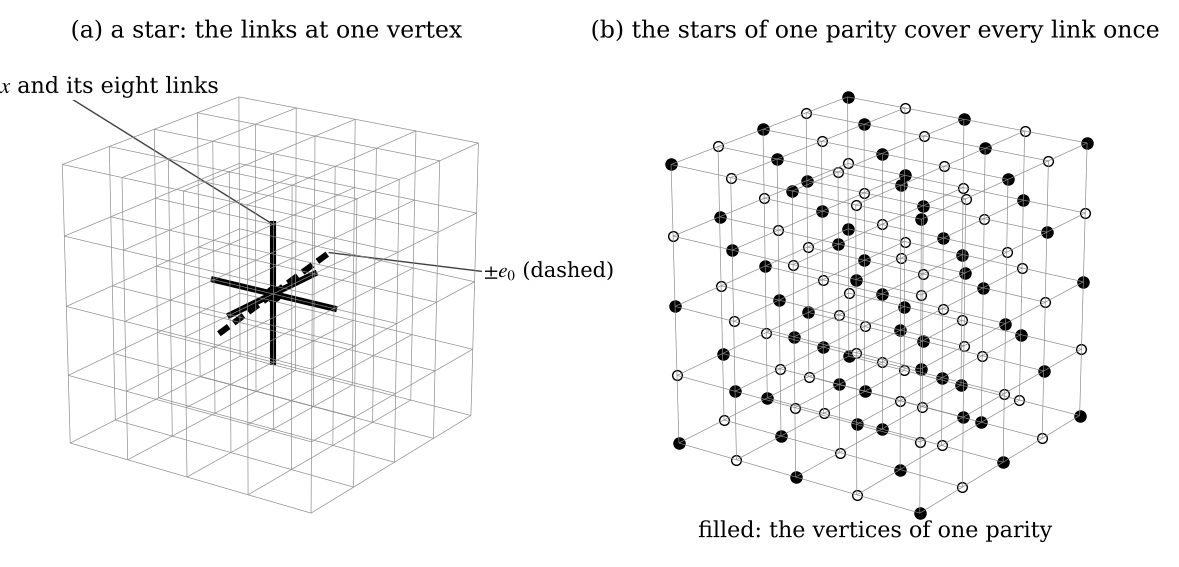
\includegraphics[width=\textwidth]{figures/fig_star.png}
\caption{(a) A star: the eight links at a vertex $x$ of the four-dimensional lattice, three spatial pairs drawn as axes and the pair $\pm e_0$ as a dashed stub. (b) The vertices of one parity (filled) on a three-dimensional slice of a torus of even side: every link has exactly one end point of each parity, so the stars of one parity partition the links and no plaquette is internal to a star.}
\label{fig:star}
\end{figure}

\emph{Setting.} Throughout the section $G=\SU(2)$, identified with the unit
quaternions $S^3\subset\R^4$, with the Euclidean inner product
$\ip\cdot\cdot$ of $\R^4$ and the chordal metric $\delta(U,V)=|U-V|$, which is
bi-invariant, invariant under inversion, and of diameter $2$. For unit
quaternions $\ReTr U=2\ip U1$, and for unit $p,q$ and $x,y\in\R^4$,
$\ip{px}y=\ip x{\bar py}$, $\ip{xq}y=\ip x{y\bar q}$ and $|pxq|=|x|$. The
Wilson measure is $\mu(dU)=Z^{-1}\prod_pe^{2\beta\ReTr U_p}\prod_edU_e$ on
$\Lambda_L$, $L$ even, with $\beta_W=4\beta$, and $\mathcal A$, $V_x$,
$\mathcal P_x$ and $\BP(n,\varpi)$ are as in Sec.~\ref{sec:cube}. For a set
$V$ of links, $\mathcal P_V$ is the conditional expectation given the links
outside $V$. For $b\in\R^4$, $\nu_b(dx)\propto e^{\ip xb}dx$ is the von
Mises--Fisher law on $S^3$, and the sharp quarter (Theorem~\ref{q-thm:quarter}
in Appendix~\ref{app:sharp}) states
\begin{equation}\label{eq:Q}
W_1(\nu_b,\nu_{b'})\le\theta\,|b-b'|\quad\text{for all }b,b'\in\R^4,
\qquad\theta=\tfrac14,
\end{equation}
with $W_1$ the Kantorovich distance for $\delta$. This is the only property of
$\nu_b$ used in the section. We put
\[
c=4\theta|\beta|=|\beta|=\tfrac14|\beta_W| .
\]
Every argument below uses only~\eqref{eq:Q}, and with a constant $\theta$ in
place of $\frac14$ the ranges become $4\theta|\beta|\le\frac7{80}$ and
$4\theta|\beta|\le\frac9{100}$.

\subsection{Even stars and two-paths}

Call a vertex \emph{even} if the sum of its coordinates is even. For an even
vertex $v$ the \emph{star} $B_v$ is the set of the eight links with an end
point at $v$. Write the eight directions as $\pm1,\dots,\pm4$, and for the link
of $B_v$ in direction $\sigma$ let $X_\sigma$ be its parallel transporter from
$v$ outwards: $X_{+\mu}=U_{(v,\mu)}$ and $X_{-\mu}=U_{(v-e_\mu,\mu)}^{-1}$. Two
directions are \emph{adjacent} if they are distinct and not opposite; each
direction is adjacent to six others, and there are $24$ adjacent pairs.

\begin{lemma}\label{lem:stars}
Let $L\ge4$ be even.
\begin{enumerate}[label=\textup{(\roman*)},leftmargin=*]
\item Every link has exactly one even end point, so the stars partition $E$.
\item Every plaquette has exactly two even corners $v,v'$, which are opposite
corners, and two of its links lie in $B_v$, two in $B_{v'}$. The plaquettes
with corner $v$ correspond bijectively to the adjacent pairs $\{\sigma,\tau\}$:
the plaquette $p_{\sigma\tau}$ has corners $v$, $v+\sigma$, $v+\sigma+\tau$,
$v+\tau$.
\item For such a plaquette, $\ReTr U_p=2\ip{h_p}{X_\sigma^{-1}X_\tau}$, where
the \emph{two-path} $h_p$ is the transporter from $v+\sigma$ to $v+\tau$
through the opposite even corner $v'=v+\sigma+\tau$, the product of the two
links of $p$ in $B_{v'}$, suitably inverted. $h_p$ is unchanged by a gauge
transformation at $v'$, and changing one of its two links by $\eta$ in
$\delta$ changes $h_p$ by exactly $\eta$.
\item The conditional law of $(X_\sigma)_\sigma$ given the links outside $B_v$ is
\[
\gamma_{v,h}(dX)=\frac1{Z_v}\prod_{\{\sigma,\tau\}}e^{4\beta\ip{h_{\sigma\tau}}
{X_\sigma^{-1}X_\tau}}\prod_\sigma dX_\sigma ,
\]
with one ordering fixed in each adjacent pair. It depends on the
configuration only through the $24$ two-paths $h=(h_{\sigma\tau})$, and it is
invariant under $X_\sigma\mapsto gX_\sigma$, the gauge transformation at $v$.
\item A link $i$ with even end point $v_i$ lies in exactly six plaquettes;
their even corners other than $v_i$ are six distinct even vertices, and for
each of them, $v$, the link $i$ is a factor of exactly one two-path $h_p$ with
$p$ at $v$.
\end{enumerate}
\end{lemma}

\begin{proof}
(i) The end points of a link differ by a unit vector, so their parities
differ. (ii) The corners of a plaquette are $y$, $y+e_\mu$, $y+e_\mu+e_\nu$,
$y+e_\nu$, of parities $\epsilon,\epsilon+1,\epsilon,\epsilon+1$, and each
link joins consecutive corners. A plaquette with even corner $v$ is spanned by
two adjacent directions at $v$, and conversely; since $L\ge4$ these $24$
squares are distinct. (iii) Going around $p$ from $v$, $U_p$ is conjugate to
$X_\sigma h_pX_\tau^{-1}$ or to its inverse, and $\ReTr$ is a class function,
invariant under inversion on $\SU(2)$; so $\ReTr U_p=\ReTr(X_\sigma h_p
X_\tau^{-1})=2\ip{X_\sigma h_p}{X_\tau}=2\ip{h_p}{X_\sigma^{-1}X_\tau}$. A gauge
transformation $g$ at $v'$ multiplies the first factor of $h_p$ on the right
by $g^{-1}$ and the second on the left by $g$, and multiplication by unit
quaternions is an isometry. (iv) The plaquettes containing a link of $B_v$
are those with corner $v$, by (ii), and their weights are given by (iii); the
gauge transformation at $v$ changes no two-path. (v) If $i$ joins $v_i$ to
$w=v_i+\sigma$, its plaquettes are spanned by $\sigma$ and the six directions
$\tau\perp\sigma$, with opposite even corners $v_i+\sigma+\tau$, which are
distinct since $L\ge4$; in the plaquette with corner $v$, the link $i$ is one
of the two links at $v_i$, hence a factor of the two-path.
\end{proof}

For the star at $v$ define the quotient pseudometric
\[
\bar d_v(X,X')=\min_{g\in G}\sum_\sigma\delta(gX_\sigma,X'_\sigma).
\]

\subsection{The seven-spin system}

Fix an adjacent pair $\{a,b\}$, let $S_a$ be the set of the seven directions
other than $a$, $A_7$ its adjacency matrix and $e_b$ the indicator of $b$.
In $S_a$, the direction $b$ is adjacent to $\bar a=-a$ and to the four
directions $C$ of the other two axes; $\bar a$ is adjacent to $b$,
$\bar b=-b$ and $C$; $\bar b$ to $\bar a$ and $C$; and each element of $C$ to
$b$, $\bar a$, $\bar b$ and the two elements of $C$ on the other axis. The
largest degree is $6$. For $0\le c<\frac16$ put
\[
s(c)=\mathbf 1^{\mathsf T}(I-cA_7)^{-1}e_b=\sum_{k\ge0}c^k\,\mathbf 1^{\mathsf T}
A_7^ke_b ,
\]
a nondecreasing function of $c$ with $s(c)\ge1$. The symmetries fixing $a$ and
$b$ permute $C$ transitively, so $x=(I-cA_7)^{-1}e_b$ is constant, equal to
$z$, on $C$, and $(x_b,x_{\bar a},x_{\bar b},z)$ is the unique solution of
\begin{equation}\label{eq:sevensys}
\begin{aligned}
x_b&=1+c(x_{\bar a}+4z),&\quad x_{\bar a}&=c(x_b+x_{\bar b}+4z),\\
x_{\bar b}&=c(x_{\bar a}+4z),&\quad z&=c(x_b+x_{\bar a}+x_{\bar b}+2z),
\end{aligned}
\end{equation}
with $s(c)=x_b+x_{\bar a}+x_{\bar b}+4z$.

\begin{lemma}\label{lem:svalues}
\begin{enumerate}[label=\textup{(\roman*)},leftmargin=*]
\item $s(\frac1{12})=\frac{26}{15}$, with $(x_b,x_{\bar a},x_{\bar b},z)=
\frac1{210}(221,28,11,26)$.
\item $s(\frac7{80})=\frac{3480}{1933}$, with $(x_b,x_{\bar a},x_{\bar b},z)=
\frac1{181702}(192531,26320,10829,24360)$.
\item $s(\frac9{100})=\frac{5450}{2957}$, with $(x_b,x_{\bar a},x_{\bar b},z)=
\frac1{348926}(371363,53100,22437,49050)$.
\end{enumerate}
Hence $6c\,s(c)$ equals $\frac{13}{15}$ at $c=\frac1{12}$, $\frac{1827}{1933}$
at $c=\frac7{80}$ and $\frac{2943}{2957}$ at $c=\frac9{100}$, and
$6c\,s(c)\le\frac{2943}{2957}$ for $0\le c\le\frac9{100}$.
\end{lemma}

\begin{proof}
Since $c\lambda_{\max}(A_7)\le6c<1$, the matrix $I-cA_7$ is invertible and it
suffices to check~\eqref{eq:sevensys}. (i) Multiplied by $12\cdot210$ the four
equations read $12\cdot221-(28+104)=2520$, $12\cdot28-(221+11+104)=0$,
$12\cdot11-132=0$ and $12\cdot26-(221+28+11+52)=0$; the sum is
$364/210=26/15$. (ii) Multiplied by $80\cdot181702=14536160$:
\begin{align*}
80\cdot192531-7(26320+4\cdot24360)&=15402480-866320=14536160,\\
80\cdot26320-7(192531+10829+4\cdot24360)&=2105600-7\cdot300800=0,\\
80\cdot10829-7(26320+4\cdot24360)&=866320-7\cdot123760=0,\\
80\cdot24360-7(192531+26320+10829+2\cdot24360)&=1948800-7\cdot278400=0.
\end{align*}
The sum is $327120/181702=3480/1933$, as $327120=94\cdot3480$ and
$181702=94\cdot1933$. (iii) Multiplied by $100\cdot348926$:
$100\cdot371363-9(53100+196200)=34892600$,
$100\cdot53100-9(371363+22437+196200)=5310000-9\cdot590000=0$,
$100\cdot22437-9(53100+196200)=0$ and
$100\cdot49050-9(371363+53100+22437+98100)=4905000-9\cdot545000=0$. The sum
is $643100/348926=5450/2957$, as $348926=118\cdot2957$ and
$643100=118\cdot5450$. The last claim follows from the monotonicity of $s$.
\end{proof}

\begin{lemma}[one star]\label{lem:onestar}
Assume~\eqref{eq:Q} and $c<\frac16$. Let $h,h'$ be two families of two-paths
at $v$ that differ only at one adjacent pair $\{a,b\}$. Then
\[
W_1^{\bar d_v}(\gamma_{v,h},\gamma_{v,h'})\le c\,s(c)\,|h_{ab}-h'_{ab}| .
\]
\end{lemma}

\begin{proof}
Under $\gamma_{v,h}$ put $Z_\sigma=X_a^{-1}X_\sigma$. The map $X\mapsto(X_a,Z)$
preserves Haar measure, and by Lemma~\ref{lem:stars}(iv) the density depends
only on $Z$, with $Z_a=1$; so $X_a$ is Haar distributed and independent of
$Z_S=(Z_\sigma)_{\sigma\in S_a}$, whose law $\mu^{(a)}_h$ has density
proportional to $\prod e^{4\beta\ip{h_{\sigma\tau}}{Z_\sigma^{-1}Z_\tau}}$. Given
a coupling of $\mu^{(a)}_h$ and $\mu^{(a)}_{h'}$, take $X_a=X'_a$ Haar and
independent, $X_\sigma=X_aZ_\sigma$ and $X'_\sigma=X_aZ'_\sigma$; this couples
$\gamma_{v,h}$ and $\gamma_{v,h'}$, and with $g=1$ in the definition,
$\bar d_v(X,X')\le\sum_{\sigma\in S_a}\delta(Z_\sigma,Z'_\sigma)$. It suffices
to bound the Kantorovich distance of $\mu^{(a)}_h$ and $\mu^{(a)}_{h'}$ for the
cost $\sum_{\sigma\in S_a}\delta$.

For $\sigma\in S_a$ the conditional law of $Z_\sigma$ given the others is
$\nu_{B_\sigma}$ with $B_\sigma=4\beta\sum_{\tau\text{ adj.\ }\sigma}w_{\sigma\tau}$,
where $w_{\sigma\tau}=Z_\tau\bar h_{\sigma\tau}$ or $Z_\tau h_{\tau\sigma}$
according to the ordering of the pair, since $\ip{h_{\sigma\tau}}{Z_\sigma^{-1}
Z_\tau}=\ip{Z_\sigma}{Z_\tau\bar h_{\sigma\tau}}$; changing $Z_\tau$ by $\eta$
changes $w_{\sigma\tau}$ by $\eta$, and changing $h_{ab}$ changes only $B_b$, by
at most $4|\beta||h_{ab}-h'_{ab}|$. Let $\pi$ minimise
$\int\sum_\sigma\delta(Z_\sigma,Z'_\sigma)\,d\pi$ over couplings of
$\mu^{(a)}_h$ and $\mu^{(a)}_{h'}$ (one exists by compactness) and put
$\varrho_\sigma=\int\delta(Z_\sigma,Z'_\sigma)\,d\pi$. Replacing
$(Z_\sigma,Z'_\sigma)$ by a measurably chosen optimal coupling of the two
conditional laws~\cite[Cor.~5.22]{Vil09} gives another coupling that changes
only the $\sigma$-term of the cost, so by minimality and~\eqref{eq:Q}
\[
\varrho_\sigma\le\theta\int|B_\sigma-B'_\sigma|\,d\pi\le c\sum_{\tau\in S_a,\
\tau\text{ adj.\ }\sigma}\varrho_\tau+c\,|h_{ab}-h'_{ab}|\,[\sigma=b],
\]
that is, $\varrho\le cA_7\varrho+c|h_{ab}-h'_{ab}|e_b$ componentwise. Iterating,
$\varrho\le\sum_{k<K}(cA_7)^kc|h_{ab}-h'_{ab}|e_b+(cA_7)^K\varrho$, and
$(cA_7)^K\to0$ since the spectral radius of $cA_7$ is at most $6c<1$.
Summing the components gives $\sum_\sigma\varrho_\sigma\le c\,s(c)|h_{ab}-
h'_{ab}|$.
\end{proof}

\subsection{The star condition and a lattice gap up to \texorpdfstring{$\beta_W=\frac9{25}$}{beta\_W=9/25}}

Let $\mathcal P_v=\mathcal P_{B_v}$ and let $N_s=L^4/2$ be the number of even
vertices. For a function $h$ on $G^E$ let $\Lip(h)$ be the least constant
with $|h(U)-h(U')|\le\Lip(h)\delta(U_i,U'_i)$ whenever $U,U'$ differ only at
one link $i$; changing links one at a time, $|h(U)-h(U')|\le\Lip(h)\sum_e
\delta(U_e,U'_e)$.

\begin{proposition}[star condition]\label{prop:starcond}
Assume~\eqref{eq:Q} and put $\gamma=c\,s(c)$, with $c<\frac16$ and $6\gamma<1$.
Then for every real $f\in\mathcal A$
\[
\sum_{v\text{ even}}\mu\bigl((f-\mathcal P_vf)^2\bigr)\ge(1-6\gamma)\Var_\mu(f).
\]
\end{proposition}

\begin{proof}
Let $h\in\mathcal A$ be Lipschitz, gauge invariant at every configuration, and
let $U,U'$ differ only at $i$. If $i\in B_v$, then $\mathcal P_vh(U)=\mathcal
P_vh(U')$. Otherwise let $\pi$ be a coupling of $\gamma_v(\cdot\mid U)$ and
$\gamma_v(\cdot\mid U')$ minimising the integral of $\bar d_v$, a continuous
pseudometric on a compact space. For $\sigma,\sigma'\in G^{B_v}$ and $g\in G$
the gauge transformation $g$ at $v$ changes only the links of $B_v$, so by
gauge invariance $h(\sigma',U')=h(g\sigma',U')$ and
\[
|h(\sigma,U)-h(\sigma',U')|\le\Lip(h)\Bigl(\sum_{e\in B_v}\delta(\sigma_e,
(g\sigma')_e)+\delta(U_i,U'_i)\Bigr);
\]
the infimum over $g$ gives $\Lip(h)(\bar d_v(\sigma,\sigma')+\delta(U_i,U'_i))$.
By Lemma~\ref{lem:stars}(iv),~(v), the laws $\gamma_v(\cdot\mid U)$ and
$\gamma_v(\cdot\mid U')$ differ only through the two-path of one plaquette,
which moves by $\delta(U_i,U'_i)$, if $v$ is one of the six vertices of
Lemma~\ref{lem:stars}(v), and coincide otherwise. Lemma~\ref{lem:onestar}
gives
\[
|\mathcal P_vh(U)-\mathcal P_vh(U')|\le\Lip(h)\,\bigl(1+\gamma\,[v\text{ one of
the six}]\bigr)\,\delta(U_i,U'_i).
\]
For $\mathcal K_s=N_s^{-1}\sum_v\mathcal P_v$, summing over $v$ (exactly one
star contains $i$) gives $\Lip(\mathcal K_sh)\le(1-\kappa_0)\Lip(h)$ with
$\kappa_0=(1-6\gamma)/N_s$. Each $\mathcal P_v$ maps $\mathcal A$ to itself, by
gauge covariance of $\gamma_v$, and for a Lipschitz $g\in\mathcal A$,
$\Var_\mu(g)\le\frac12\iint(g(U)-g(U'))^2\,\mu(dU)\mu(dU')\le2\Lip(g)^2|E|^2$.
So $\Var_\mu(\mathcal K_s^th)\le2(1-\kappa_0)^{2t}\Lip(h)^2|E|^2$. On the
mean-zero part of $\mathcal A$ the operator $\mathcal K_s$ is self-adjoint with
$0\le\mathcal K_s\le I$, and $\Var_\mu(\mathcal K_s^th)=\int\lambda^{2t}\,
d\nu_h(\lambda)$ for its spectral measure $\nu_h$ at $h-\mu(h)$; hence $\nu_h$
lives on $[0,1-\kappa_0]$. Lipschitz functions are dense in $L^2(\mu)$, and
the orthogonal projection onto $\mathcal A$, averaging over the compact gauge
group, which acts link by link by isometries, does not increase $\Lip$; so
such $h$ are dense in $\mathcal A$, and the spectral projection of $\mathcal K_s$
on $(1-\kappa_0,1]$ vanishes on the mean-zero part of $\mathcal A$. Thus
$\ip f{(I-\mathcal K_s)f}\ge\kappa_0\Var_\mu(f)$, and $\ip f{(I-\mathcal P_v)f}=
\mu((f-\mathcal P_vf)^2)$.
\end{proof}

\begin{theorem}\label{thm:stars}
Let $G=\SU(2)$ and $|\beta_W|\le\frac9{25}$. Then for every even $L\ge4$ and
every real $f\in\mathcal A$,
\[
\sum_{v\text{ even}}\mu\bigl((f-\mathcal P_vf)^2\bigr)\ge\frac{14}{2957}
\Var_\mu(f),
\]
and for every $n\ge2$ and even $L\ge2n+4$, $\BP(n,\varpi_n)$ holds with
\[
\varpi_n=\frac{14}{2957}\cdot\frac{(n-1)^4}{n^4\lceil(n-1)^4/2\rceil},\qquad
\varpi_2=\frac{14}{16\cdot2957}.
\]
For $0\le\beta_W\le\frac9{25}$ every torus limit is translation invariant and
reflection positive, and its transfer matrix has spectral gap at least
$\varpi_2/(2e^2q_2)=7/(625\cdot2957\,e^2)$.
\end{theorem}

\begin{proof}
Here $c=|\beta|\le\frac9{100}$, and by Lemma~\ref{lem:svalues}
$1-6c\,s(c)\ge\frac{14}{2957}$; the first claim is
Proposition~\ref{prop:starcond}. For a cube $V_x$, an even vertex $v$ with
$v-x\in[1,n-1]^4$ has its eight links based in $x+[0,n)^4$, so $B_v\subset
V_x$. The $\sigma$-algebra of the links outside $V_x$ is contained in that of
the links outside $B_v$, so $\mu((f-\mathcal P_xf)^2)=\mu(f^2)-\mu((\mathcal
P_xf)^2)\ge\mu(f^2)-\mu((\mathcal P_vf)^2)=\mu((f-\mathcal P_vf)^2)$. Each cube
contains at most $N=\lceil(n-1)^4/2\rceil$ such vertices, and each even $v$ is
in this position in exactly $(n-1)^4$ cubes. Averaging over those $v$ in each
cube,
\[
\sum_x\mu((f-\mathcal P_xf)^2)\ge\frac{(n-1)^4}{N}\sum_{v\text{ even}}
\mu((f-\mathcal P_vf)^2)\ge\frac{(n-1)^4}N\cdot\frac{14}{2957}\Var_\mu(f),
\]
which is $\BP(n,\varpi_n)$. The last claim is Corollary~\ref{cor:latticegap}
with $n=2$ and $q_2=\frac{625}{16}$.
\end{proof}

The same proof works whenever $6c\,s(c)<1$. The exact threshold is the root
$c_*$ of $6c\,s(c)=1$, and Lemma~\ref{lem:svalues}(iii) shows
$c_*>\frac9{100}$.\footnote{Solving~\eqref{eq:sevensys} numerically gives
$c_*\approx0.09023$, that is $\beta_W\approx0.3609$. No statement of the paper
uses this value.} At $\beta_W=\frac13$ the star condition holds with
$6c\,s(c)=\frac{13}{15}$, while the single-link argument of
Sec.~\ref{sec:bpstrong} is exactly marginal there. The constant $\varpi_n$ of
Theorem~\ref{thm:stars} decays like $\frac{28}{2957}n^{-4}$, so that theorem is
a cube condition for each fixed $n$, enough for the lattice gap but not for
Theorem~\ref{thm:B}. The lower faces of a cube are the reason, and the next
proposition shows that they stop every certificate that treats their links
one at a time.

\begin{proposition}[the face barrier]\label{prop:facebarrier}
For a lower face $\{\hat v_i=0\}$ of the cube $V_x$, $\hat v=v-x$, let $F_i$ be
the set of links $(b,\mu)\in V_x$ with $\hat b_i=0$ and $\mu\ne i$, and let
$A_F$ be the matrix on $F_i$ with $(A_F)_{ek}=1$ when $e\ne k$ lie in a common
plaquette all of whose links are in $F_i$. Then $\lambda_{\max}(A_F)\ge
12(1-\frac1n)^2$. Consequently, if a certificate for the response of a cube
treats the links of $F_i$ as single sites with influence matrix $C\ge cA_F$ on
$F_i\times F_i$, the inequalities $0\le\varrho\le C\varrho+\mathfrak s$ admit
solutions with $\sum\varrho$ arbitrarily large as soon as
$12c(1-\frac1n)^2\ge1$; as $n\to\infty$ such a certificate cannot pass
$c=\frac1{12}$, that is $|\beta_W|=\frac13$.
\end{proposition}

\begin{proof}
$|F_i|=3n^3$. A plaquette in a plane $\{\mu,\nu\}\not\ni i$ with base point
$y$, $\hat y_i=0$, has all four links in $F_i$ exactly when its three base
points lie in $x+[0,n)^4$, that is $\hat y_\mu,\hat y_\nu\le n-2$; there are
$3n(n-1)^2$ of them. Two links share at most one plaquette, so
$\mathbf 1^{\mathsf T}A_F\mathbf 1=12\cdot3n(n-1)^2$, and the Rayleigh quotient
of $\mathbf 1$ is $12(1-\frac1n)^2$. If $c\lambda_{\max}(A_F)\ge1$ and $w\ge0$
is a Perron vector of $A_F$, extended by $0$, then $\varrho=tw$ satisfies
$C\varrho\ge tcA_Fw\ge\varrho$ on $F_i$ for every $t>0$.
\end{proof}

For single-link updates the hypothesis $C\ge cA_F$ holds with $c=|\beta|$: at
$b=0$ the derivative of $b\mapsto\nu_b$ has Kantorovich norm exactly
$\frac14$ (Lemma~\ref{q-lem:rate}(i)), and the staples of a face link can
cancel while one of them moves. The forest of Sec.~\ref{sec:bpstrong} does not
help, since its links $T_x$ have interior heads and the face links are free.
What does help is to let the gauge transformation act at the vertices of the
faces as well, and to pay for it.

\subsection{The cube as a block system}

Fix $x$ and $n\ge2$, and write $\hat v=v-x$, computed in a window
$x+[-2,n+2]^4$ that embeds in $\Z^4$ because $L\ge2n+4$. Let $V=V_x$ and
$Q=\{v:\hat v\in[0,n-1]^4\}$. Call $v$ \emph{lower} if $v\in Q$, with zero set
$Z(v)=\{a:\hat v_a=0\}$ and $z(v)=|Z(v)|$, and \emph{upper} if $\hat v\in
[0,n]^4$ has exactly one coordinate equal to $n$. If $k$ is a link with odd end
point $o$ and direction $\mu$, its six plaquettes are indexed by $(\nu,
\epsilon)$, $\nu\ne\mu$, $\epsilon=\pm1$; the even corner of the plaquette
$(\nu,\epsilon)$ other than the even end point of $k$ is $o+\epsilon e_\nu$,
and there $k$ is a factor of the two-path of this plaquette only
(Lemma~\ref{lem:stars}(v)).

\begin{lemma}\label{lem:cubestars}
Let $n\ge2$.
\begin{enumerate}[label=\textup{(\roman*)},leftmargin=*]
\item If $v$ is lower and even, $B_v\cap V$ consists of $B_v$ minus the
$z(v)$ \emph{outside links} $(v-e_a,a)$, $a\in Z(v)$; we call the directions
$-a$, $a\in Z(v)$, \emph{fixed} and the others \emph{free}. If $v$ is upper
and even with $\hat v_a=n$, then $B_v\cap V=\{(v-e_a,a)\}$. Other even vertices
carry no link of $V$. Hence $V$ is partitioned into the \emph{blocks}
$B_v\cap V$, $v$ even and lower or upper, and the \emph{owner} $w(k)$ of
$k\in V$ is its even end point.
\item Let $k\in V$ have odd end point $o$, direction $\mu$ and owner
$o+\varsigma e_\mu$, $\varsigma=\pm1$, and let $p$ be its plaquette
$(\nu,\epsilon)$, $v=o+\epsilon e_\nu$. The links of $p$ at $v$ are in the
directions $-\epsilon\nu$ and $\varsigma\mu$. If $v$ is lower, both lie in
$V$. If $v$ is upper with $\hat v_a=n$, the links of $p$ at $v$ other than
$(v-e_a,a)$ lie outside $V$.
\item Let $v$ be lower and even and $a\in Z(v)$. The outside link $(v-e_a,a)$
is a factor of no two-path $h_p$ at a lower or upper vertex. If a plaquette
$p$ at $v$ has one of its links at $v$ outside $V$, then both links of $p$ at
the opposite even corner lie outside $V$.
\end{enumerate}
\end{lemma}

\begin{proof}
(i) The outgoing links $(v,b)$ of a lower $v$ have base point in $Q$, and an
incoming link $(v-e_b,b)$ lies in $V$ if and only if $\hat v_b\ge1$. If
$\hat v_a=n$ for exactly one $a$, no outgoing link and no incoming link
$(v-e_b,b)$, $b\ne a$, has its base point in $Q$, while $(v-e_a,a)$ has. If
$\hat v\notin[0,n]^4$ or two coordinates equal $n$, no link at $v$ has its base
point in $Q$.

(ii) The corners of $p$ are $o$, $o+\varsigma e_\mu$, $o+\varsigma e_\mu+
\epsilon e_\nu$ and $v$, so the links at $v$ go to $o$, in direction
$-\epsilon\nu$, and to $v+\varsigma e_\mu$, in direction $\varsigma\mu$. Let $v$
be lower. If $\epsilon=+1$ the first link is $(o,\nu)$, and $\hat o=\hat v-e_\nu$
lies in $Q$, its $\nu$-coordinate being $\hat o_\nu\ge0$; if $\epsilon=-1$ it is
$(v,\nu)$, with base point $v\in Q$. The second link is $(v,\mu)$ if
$\varsigma=+1$; if $\varsigma=-1$ it is $(v-e_\mu,\mu)$, which lies in $V$
because $\hat v_\mu=\hat o_\mu\ge1$, as $k=(o-e_\mu,\mu)\in V$. If $v$ is upper,
(i) gives the claim.

(iii) The plaquettes of $(v-e_a,a)$ have the even corners $v$ and
$v-e_a\pm e_\nu$, whose $a$-coordinate is $-1$, so these are neither lower nor
upper; and a link is a factor of a two-path only at the even corner opposite
to its own even end point. If $p$ at $v$ is spanned by $-a$ and $\tau$, the
opposite corner $v'=v-e_a+\tau$ and both its neighbours in $p$, $v-e_a$ and
$v+\tau$, are joined to it by links based at $a$-coordinate $-1$.
\end{proof}

For a block vertex $v$ the conditional law $\gamma_v(\cdot\mid\sigma,U)$ of
the links of $B_v\cap V$, given the other links of $V$ (values $\sigma$) and
the links off $V$ (values $U$), has density proportional to the product of
the weights $e^{4\beta\ip{h_p}{X_\sigma^{-1}X_\tau}}$ of the plaquettes $p$ at
$v$ with a link at $v$ in $V$. It depends on $(\sigma,U)$ only through these
two-paths and the values of the links at $v$ off $V$.

\subsection{The soft quotient}

At a vertex of a lower face the gauge transformation moves the outside links
at that vertex, and the conditional law of the cube does not see it. The
following pseudometric allows it anyway, at the price of the displacement it
causes on those links. The price is legitimate in the Lipschitz contraction
argument of Proposition~\ref{prop:interiorbp}, because the test function
depends on all links.

\begin{definition}\label{def:dtilde}
For a lower even $v$ and configurations $X,X'$ of $B_v\cap V$, written as
outward transporters, put
\[
\tilde d_v(X,X')=\min_{g\in G}\Bigl[\sum_{\sigma\text{ free}}\delta(gX_\sigma,
X'_\sigma)+z(v)\,\delta(g,1)\Bigr],
\]
and for an upper even $v$ let $\tilde d_v$ be $\delta$ on its single link. For
$\sigma,\sigma'\in G^V$ let $D(\sigma,\sigma')=\sum_v\tilde d_v(\sigma_{B_v},
\sigma'_{B_v})$, the sum over the block vertices, and for $j\notin V$
\[
\tilde R_x(j)=\sup\Bigl\{\frac{W^D(\gamma^0_{V,U},\gamma^0_{V,U'})}
{\delta(U_j,U'_j)}:U,U'\text{ differ only at }j\Bigr\},
\]
where $\gamma^0_{V,U}=\gamma^0_V(\cdot\mid U)$ and $W^D$ is the Kantorovich
distance for the cost $D$.
\end{definition}

The minimum exists by compactness, and $\tilde d_v$ and $D$ are continuous,
symmetric, since $\delta(gX,X')=\delta(X,g^{-1}X')$ and
$\delta(g,1)=\delta(g^{-1},1)$, and satisfy the triangle inequality, by
composing the minimising elements. For $z(v)=0$, $\tilde d_v=\bar d_v$.

\begin{lemma}\label{lem:softlip}
Let $h$ be a function on $G^E$, gauge invariant at every configuration, with
$|h(W)-h(W')|\le\Lip(h)\sum_e\delta(W_e,W'_e)$. If $U,U'$ differ only at
$j\notin V$, then for all $\sigma,\sigma'\in G^V$
\[
|h(\sigma,U)-h(\sigma',U')|\le\Lip(h)\bigl(D(\sigma,\sigma')+\delta(U_j,U'_j)
\bigr).
\]
\end{lemma}

\begin{proof}
For each lower even $v$ choose $g_v$ attaining $\tilde d_v(\sigma_{B_v},
\sigma'_{B_v})$, and let $g$ be the gauge transformation equal to $g_v$ at
these vertices and to $1$ elsewhere; then $h(\sigma,U)=h(g\cdot(\sigma,U))$. A
link of $V$ has exactly one even end point $v$, and $g$ acts on it by $X\mapsto
g_vX$ on its outward transporter at $v$, or trivially if $v$ is upper. A link
$e\notin V$ has at most one end point where $g\ne1$, namely an even lower
$v$, and then $e$ is one of the $z(v)$ outside links at $v$, by
Lemma~\ref{lem:cubestars}(i); there $\delta((g\cdot U)_e,U'_e)\le\delta(g_v,1)+
\delta(U_e,U'_e)$ by bi-invariance. Summing over all links,
$|h(g\cdot(\sigma,U))-h(\sigma',U')|\le\Lip(h)\bigl(\sum_v\tilde d_v+
\delta(U_j,U'_j)\bigr)$.
\end{proof}

\subsection{Block responses}

\begin{lemma}[Dobrushin on $S^3$]\label{lem:dobS3}
Assume~\eqref{eq:Q}. Let $S$ be finite and $\nu,\nu'$ probability measures on
$G^S$ with continuous positive densities with respect to Haar measure, such
that for every $s\in S$ the conditional law of $x_s$ given $x_{S\setminus s}$
is $\nu_{B_s(x)}$ under $\nu$ and $\nu_{B'_s(x)}$ under $\nu'$, where
$|B_s(x)-B_s(y)|\le4|\beta|\sum_ta_{st}\delta(x_t,y_t)$ and
$|B_s(x)-B'_s(x)|\le4|\beta|\eta_s$ for all $x,y$, with $a_{st}\ge0$,
$a_{ss}=0$ and $\eta_s\ge0$. Then there is a coupling $\pi$ of $\nu,\nu'$ whose
$\varrho_s=\int\delta(x_s,x'_s)\,d\pi$ satisfy $\varrho\le cA\varrho+c\eta$
componentwise. Consequently:
\begin{enumerate}[label=\textup{(\alph*)},leftmargin=*]
\item if $\sum_sa_{st}\le d$ for every $t$ and $cd<1$, then
$\sum_s\varrho_s\le c\sum_s\eta_s/(1-cd)$;
\item if the spectral radius of $cA$ is less than $1$ and $y\in[0,\infty)^S$
satisfies $y\ge cAy+c\eta$, then $\varrho\le y$;
\item if $y\ge0$ satisfies $y\ge c_0Ay+\eta$ and $c\le c_0$, then $cy\ge
cA(cy)+c\eta$, so $\varrho\le cy$ when the spectral radius of $cA$ is less
than $1$.
\end{enumerate}
\end{lemma}

\begin{proof}
Let $\pi$ minimise $\int\sum_s\delta(x_s,x'_s)\,d\pi$ over couplings. Fix $s$
and replace under $\pi$ the pair $(x_s,x'_s)$ by a sample of an optimal
coupling of $\nu_{B_s(x)}$ and $\nu_{B'_s(x')}$, chosen measurably in
$(x_{S\setminus s},x'_{S\setminus s})$~\cite[Cor.~5.22]{Vil09}. This is again
a coupling of $\nu,\nu'$, and only the $s$-term of the cost changes, so by
minimality,~\eqref{eq:Q} and the triangle inequality, $\varrho_s\le\theta\int
|B_s(x)-B'_s(x')|\,d\pi\le c\sum_ta_{st}\varrho_t+c\eta_s$. (a) Summing over
$s$, $\sum\varrho\le cd\sum\varrho+c\sum\eta$. (b) The vector $y-\varrho$
satisfies $y-\varrho\ge cA(y-\varrho)$, hence $y-\varrho\ge(cA)^K(y-\varrho)
\to0$. (c) $cy-c^2Ay\ge c(y-c_0Ay)\ge c\eta$; apply (b).
\end{proof}

From now on $c\le c_0=\frac7{80}$, that is $|\beta_W|\le\frac7{20}$, and
$\kappa_0=s(c_0)=\frac{3480}{1933}<1.8004$, so that $6c_0\kappa_0=
\frac{1827}{1933}$. For a direction $a$ and a family $h$ of two-paths let
$\mu^{(a)}_h$ be the law on $G^{S_a}$ with density proportional to
$\prod_{\{\sigma,\tau\}}e^{4\beta\ip{h_{\sigma\tau}}{Z_\sigma^{-1}Z_\tau}}$,
$Z_a=1$, as in the proof of Lemma~\ref{lem:onestar}. By that proof,
Lemma~\ref{lem:svalues}(ii) and Lemma~\ref{lem:dobS3}(c), if $h,h'$ differ only
at the pair $\{a,b\}$ there is a coupling of $\mu^{(a)}_h$ and $\mu^{(a)}_{h'}$
with
\begin{equation}\label{eq:sevenbound}
\int\sum_{\sigma\in S_a}\delta(Z_\sigma,Z'_\sigma)\le\kappa_0c\,
|h_{ab}-h'_{ab}|\qquad(c\le c_0).
\end{equation}

\begin{lemma}\label{lem:partial}
Let $c\le c_0$ and $v$ a block vertex, and write $\gamma^{h,Y}$ for its block
law as a function of the two-paths $h$ at $v$ and of the values $Y$ of the
links at $v$ off $V$. Put $\kappa_1=\kappa_0$, $\kappa_2=\frac94$,
$\kappa_3=\frac{40}{13}$ and $\kappa_4=\frac{160}{59}$.
\begin{enumerate}[label=\textup{(\alph*)},leftmargin=*]
\item Let $v$ be lower, and let $(h,Y)$ and $(h',Y)$ differ only at the
two-path $h_p$ of a plaquette $p$ whose two links at $v$ are free. Then
$W^{\tilde d_v}(\gamma^{h,Y},\gamma^{h',Y})\le\kappa_{z(v)}c\,|h_p-h'_p|$, with
$\kappa_0$ for $z(v)=0$.
\item In particular, for $z(v)=1$ the constant is the full-star constant
$\kappa_0c$.
\item Let $v$ be lower and $p$ a plaquette at $v$ with one link at $v$ free and
one fixed. Then the bound of \textup{(a)} holds with $\kappa_0c$ if $z(v)=1$
and with $\frac{16}9c$ if $z(v)\ge2$.
\item Let $v$ be lower and let $(h,Y)$ and $(h,Y')$ differ only at one
outside link, by $\eta$ in $\delta$. Then $W^{\tilde d_v}(\gamma^{h,Y},
\gamma^{h,Y'})\le\eta$.
\item Let $v$ be upper. If $(h,Y)$ and $(h',Y')$ differ only at one two-path
$h_p$ with $p\ni(v-e_a,a)$, or only at one outside link at $v$, the distance is
at most $c|h_p-h'_p|$, respectively $c\eta$.
\end{enumerate}
\end{lemma}

\begin{proof}
\emph{Representation.} Let $v$ be lower and $F$ its set of fixed directions,
let $\Phi_h(X)=\prod e^{4\beta\ip{h_{\sigma\tau}}{X_\sigma^{-1}X_\tau}}$ over all
$24$ adjacent pairs, so that $\Phi_h(gX)=\Phi_h(X)$, and note that
$\gamma^{h,Y}$ has density proportional to $\Phi_h$ evaluated at $X_F=Y_F$. Fix
a free direction $\sigma_0$. If $F=\emptyset$, the map
$X\mapsto(X_{\sigma_0},(X_{\sigma_0}^{-1}X_\rho)_{\rho\ne\sigma_0})$ preserves
Haar measure and carries $\gamma^h$ to $\mathrm{Haar}\otimes\mu^{(\sigma_0)}_h$,
as in the proof of Lemma~\ref{lem:onestar}. If $F\ne\emptyset$, fix $f_1\in F$
and let $\Psi(X)$ consist of $W_\rho=X_{\sigma_0}^{-1}X_\rho$ for the free
$\rho\ne\sigma_0$ and of $W_m=X_{\sigma_0}^{-1}Y_{f_1}$. Then $\Psi$ is a
bijection of the free coordinates, with inverse $X_{\sigma_0}=Y_{f_1}W_m^{-1}$,
$X_\rho=Y_{f_1}W_m^{-1}W_\rho$, and it preserves Haar measure: $X_{\sigma_0}
\mapsto X_{\sigma_0}^{-1}Y_{f_1}$ does, and for fixed $X_{\sigma_0}$ so does
each $X_\rho\mapsto X_{\sigma_0}^{-1}X_\rho$. Since $\Phi_h(X)=\Phi_h(
X_{\sigma_0}^{-1}X)$ and $X_{\sigma_0}^{-1}X_f=W_mK_f$ with $K_f=Y_{f_1}^{-1}
Y_f$, the image of $\gamma^{h,Y}$ has density proportional to $\Phi_h$ at
$X_{\sigma_0}=1$, $X_\rho=W_\rho$, $X_f=W_mK_f$. If $(W,W')$ couples the images
for $(h,Y)$ and $(h',Y)$ and $X=\Psi^{-1}W$, $X'=\Psi^{-1}W'$, then
$g=Y_{f_1}W'^{-1}_mW_mY_{f_1}^{-1}$ satisfies $gX_{\sigma_0}=X'_{\sigma_0}$,
$\delta(gX_\rho,X'_\rho)=\delta(W_\rho,W'_\rho)$ and $\delta(g,1)=
\delta(W_m,W'_m)$, so
\begin{equation}\label{eq:transfer}
\tilde d_v(X,X')\le\sum_\rho\delta(W_\rho,W'_\rho)+z(v)\,\delta(W_m,W'_m).
\end{equation}

(a), (b) for $z(v)\le1$. Take $\sigma_0$ and $\tau$ to be the two directions of
$p$ at $v$. For $z(v)=1$, $F=\{f_1\}$, the image is exactly
$\mu^{(\sigma_0)}_h$, the coordinate $W_m$ being $Z_{f_1}$, and the change of
$h_p=h_{\sigma_0\tau}$ is a change of the field on $Z_\tau$;
\eqref{eq:sevenbound} and~\eqref{eq:transfer} give $\kappa_0c|h_p-h'_p|$. For
$z(v)=0$ couple with the same $X_{\sigma_0}$ and use $g=1$; this is
Lemma~\ref{lem:onestar} with~\eqref{eq:sevenbound}.

(a) for $z(v)=2$. Let $F=\{-i,-j\}$; the free directions are $P=+i$, $Q=+j$,
$K_\pm=\pm k$ and $L_\pm=\pm l$. Up to the symmetries $i\leftrightarrow j$,
$k\leftrightarrow l$, $k\mapsto-k$ and $l\mapsto-l$ of the star, which fix
$F$, the pair of $p$ is one of $\{P,Q\}$, $\{P,K_+\}$ and $\{K_+,L_+\}$. In the
image the terms of the density are: for adjacent free $\rho,\rho'\ne\sigma_0$,
$\ip h{W_\rho^{-1}W_{\rho'}}$; for $\{\sigma_0,\rho\}$, a field on $W_\rho$; for
$\{f,\rho\}$, $\ip h{(W_mK_f)^{-1}W_\rho}=\ip{K_fh}{W_m^{-1}W_\rho}$, linear in
$W_m$ and in $W_\rho$; for $\{\sigma_0,f\}$, a field on $W_m$; and for
$\{-i,-j\}$, a constant. So Lemma~\ref{lem:dobS3} applies with
$a_{\rho\rho'}=1$ for adjacent free $\rho,\rho'\ne\sigma_0$,
$a_{\rho m}=a_{m\rho}$ equal to the number of $f\in F$ adjacent to $\rho$
(one for $P,Q$, two for $K_\pm,L_\pm$), and $\eta=|h_p-h'_p|e_\tau$. Every row
sum of $A$ is at most $9$, so $c_0A$ has spectral radius at most
$\frac{63}{80}$. By~\eqref{eq:transfer} the cost is at most
$\sum_\rho\varrho_\rho+2\varrho_m$. We give $\hat y\ge c_0A\hat y+e_\tau$ and
use Lemma~\ref{lem:dobS3}(c); each item lists $\hat y$ and the inequalities
multiplied by $80$ and by the denominator of $\hat y$.

\emph{The pair $\{P,Q\}$}, $\sigma_0=P$, $\tau=Q$. The spins are $Q$, $K_\pm$,
$L_\pm$, each of the last four adjacent to $Q$ and to the two of the other
axis, and $m$; $100\hat y=(Q,K_\pm,L_\pm,m)=(108,16,21)$. The inequalities
are $8640\ge7(4\cdot16+21)+8000=8595$, $1280\ge7(108+2\cdot16+2\cdot21)=1274$
and $1680\ge7(108+8\cdot16)=1652$, and the cost is at most
$(108+4\cdot16+2\cdot21)/100=2.14$.

\emph{The pair $\{P,K_+\}$}, $\sigma_0=K_+$, $\tau=P$. The spins are $P$ and
$Q$, adjacent to each other and to $K_-$, $L_\pm$; $K_-$, adjacent to $P,Q,
L_\pm$; $L_\pm$, adjacent to $P,Q,K_-$; and $m$; $200\hat y=(P,Q,K_-,L_\pm,m)=
(216,32,35,32,40)$. The inequalities are $17280\ge7(32+35+64+40)+16000=17197$,
$2560\ge7(216+35+64+40)=2485$, $2800\ge7(216+32+64+80)=2744$,
$2560\ge7(216+32+35+80)=2541$ and $3200\ge7(216+32+70+128)=3122$, and the
cost is at most $(216+32+35+64+80)/200=2.135$.

\emph{The pair $\{K_+,L_+\}$}, $\sigma_0=K_+$, $\tau=L_+$, with the same spins
and adjacencies; $200\hat y=(P,Q,K_-,L_+,L_-,m)=(32,32,36,219,19,54)$. The
inequalities are $2560\ge7(32+36+219+19+54)=2520$ for $P$ and for $Q$,
$2880\ge7(64+219+19+108)=2870$, $17520\ge7(64+36+108)+16000=17456$,
$1520\ge7(64+36+108)=1456$ and $4320\ge7(64+72+2\cdot238)=4284$, and the cost
is at most $(64+36+219+19+108)/200=2.23$.

In all cases the response is at most $2.23\,c|h_p-h'_p|\le\kappa_2c|h_p-h'_p|$.

(a) for $z(v)\ge3$, and (c), (d) for $z(v)\ge2$. Use the coordinates
$X_\sigma$, $\sigma$ free, directly, and $g=1$ in $\tilde d_v$. Each conditional
law is $\nu_B$ with $B=4\beta$ times the sum of the unit vectors of the
plaquettes at $v$ through $\sigma$, those through free neighbours depending
isometrically on them; so Lemma~\ref{lem:dobS3}(a) applies with $A$ the
adjacency matrix of the free directions, whose largest degree is $d=5,4,3$
for $z(v)=2,3,4$ (for $z=2$, $+i$ is adjacent to $+j$, $\pm k$, $\pm l$; for
$z=3$, $+i$ to $+j$, $+k$, $\pm l$; for $z=4$ the free directions are the four
positive ones). A change of $h_p$ with both links free gives $\sum\eta=
2|h_p-h'_p|$, with one link free $\sum\eta=|h_p-h'_p|$, and a change of the
outside link in direction $f$ by $\eta$ gives $\eta$ on each free neighbour of
$f$, at most $d$ of them. With $c\le c_0$: $\frac{2c}{1-4c}\le\frac{40}{13}c$,
$\frac{2c}{1-3c}\le\frac{160}{59}c$, $\frac c{1-cd}\le\frac c{1-5c_0}=
\frac{16}9c$ and $\frac{dc}{1-dc}\le\frac{5c_0}{1-5c_0}=\frac79$.

(c), (d) for $z(v)=1$. Let $F=\{f\}$ and $X_f=Y$. The map $X\mapsto Z=(Y^{-1}
X_\rho)_\rho$ carries $\gamma^{h,Y}$ to $\mu^{(f)}_h$, which does not depend on
$Y$. A change of $h_p$, $p$ spanned by $f$ and $\tau$, is a change of the
field on $Z_\tau$, so~\eqref{eq:sevenbound} gives a coupling with
$\int\sum\delta(YZ_\rho,YZ'_\rho)\le\kappa_0c|h_p-h'_p|$, with $g=1$. For a
change $Y\to Y'$ couple $X=YZ$ and $X'=Y'Z$ and take $g=Y'Y^{-1}$; then
$\tilde d_v(X,X')\le\delta(Y'Y^{-1},1)=\delta(Y,Y')$.

(e) The block law is $\nu_b$ with $b=4\beta$ times the sum of the six vectors
of the plaquettes through $(v-e_a,a)$; such a change moves $b$ by at most
$4|\beta||h_p-h'_p|$, respectively $4|\beta|\eta$, since an outside link lies
in at most one plaquette with $(v-e_a,a)$. Apply~\eqref{eq:Q}.
\end{proof}

Part (b) is the point of the soft quotient: a star with one fixed link is
exactly as good as a full star, and the price $z(v)\delta(g,1)$ never feeds
back into the system, because an outside link of a lower vertex is a factor
of no two-path at a block (Lemma~\ref{lem:cubestars}(iii)). The margin is lost
at the edges of the cube, $z(v)=2$, and the next lemma pays for them with
weights.

\subsection{The column inequality}

For a block vertex $v$ and a plaquette $p$ at $v$ let $\Gamma_v(p)$ be the
constant of Lemma~\ref{lem:partial}(a), (c) or (e), and $\Gamma_v(p)=0$ if no
link of $p$ at $v$ lies in $V$. Put $u_v=1$ for upper $v$ and $u_v=u_{z(v)}$
for lower $v$, with
\[
u_0=u_1=1,\quad u_2=\tfrac56,\quad u_3=\tfrac7{10},\quad u_4=\tfrac35;
\qquad\lambda=\tfrac{97}{100}.
\]

\begin{lemma}\label{lem:column}
Let $n\ge4$ and $c\le c_0$. For every $k\in V$, with plaquettes
$p_{(\nu,\epsilon)}$ and even corners $v_{(\nu,\epsilon)}=o+\epsilon e_\nu$ as
above,
\[
\sum_{(\nu,\epsilon)}u_{v_{(\nu,\epsilon)}}\Gamma_{v_{(\nu,\epsilon)}}
(p_{(\nu,\epsilon)})\le\lambda\,u_{w(k)} .
\]
\end{lemma}

\begin{proof}
Put $f(z)=u_z\kappa_zc$: $f(0)=f(1)=\kappa_0c<1.8004\,c$, $f(2)=\frac{15}8c$,
$f(3)=\frac{28}{13}c<2.1539\,c$ and $f(4)=\frac{96}{59}c<1.6272\,c$, all at
least $c$. By Lemma~\ref{lem:cubestars}(ii) a lower $v_{(\nu,\epsilon)}$ has
both links of $p$ free, so it contributes $f(z(v_{(\nu,\epsilon)}))$; an upper
one contributes at most $c$, and other vertices contribute $0$. Let $o$, $\mu$
and $\varsigma$ be as in Lemma~\ref{lem:cubestars}(ii).

\emph{Case A: $\hat o$ has a coordinate equal to $n$.} Since $k\in V$ is
$(o,\mu)$, which needs $o\in Q$, or $(o-e_\mu,\mu)$, which needs $\hat o-e_\mu
\in[0,n-1]^4$, this coordinate is $\hat o_\mu$, and $w(k)=o-e_\mu$ with
$\hat w_\mu=n-1\ge1$; so $z(w)\le3$ and $u_w\ge\frac7{10}$. Every
$v_{(\nu,\epsilon)}$ has $\mu$-coordinate $n$, so the sum is at most
$6c\le6c_0=0.525<\frac7{10}\cdot0.97$.

\emph{Case B: $o\in Q$.} Let $Z=z(o)$ be the number of zeros of $\hat o$,
$a=\#\{\nu\ne\mu:\hat o_\nu=0\}$ and $b=\#\{\nu\ne\mu:\hat o_\nu=1\}$. As
$n\ge4$, the classes $\{0\}$, $\{1\}$, $[2,n-2]$ and $\{n-1\}$ are disjoint.
For $\nu\ne\mu$: if $\hat o_\nu=0$, $\epsilon=-1$ gives no block and
$\epsilon=+1$ a lower vertex with $z=Z-1$; if $\hat o_\nu=1$, $\epsilon=+1$
gives $z=Z$ and $\epsilon=-1$ gives $z=Z+1$; if $2\le\hat o_\nu\le n-2$ both
give $z=Z$; and if $\hat o_\nu=n-1$, $\epsilon=-1$ gives $z=Z$ and
$\epsilon=+1$ an upper vertex, which contributes at most $c\le f(Z)$. Hence the
sum is at most
\[
a\,f(Z-1)+b\bigl(f(Z)+f(Z+1)\bigr)+2(3-a-b)f(Z).
\]
If $\hat o_\mu=0$, then $\varsigma=+1$, $Z=a+1$ and $z(w)=a$, and the sum is at
most $h(a,b)=af(a)+b(f(a+1)+f(a+2))+2(3-a-b)f(a+1)$, to be compared with
$\lambda u_a$. If $\hat o_\mu\ge1$, then $Z=a$ and $w$ is upper, with $u_w=1$,
or lower with $z(w)\in\{a,a+1\}$, so $u_w\ge u_{a+1}$; the sum is at most
$g(a,b)=af(a-1)+b(f(a)+f(a+1))+2(3-a-b)f(a)$, to be compared with $\lambda
u_{a+1}$. Here $a+b\le3$. Since $f(0)=f(1)\le f(2)\le f(3)$, the quantities
$h(0,b)$, $g(1,b)$, $h(1,b)$ and $g(2,b)$ increase with $b$, and
$g(0,b)=6f(0)$. Every term is $c$ times a constant, so it suffices to take
$c=c_0$; with $\hat\lambda=\lambda/c_0=\frac{388}{35}>11.0857$ and $f$ in units
of $c$, the cases are
\begin{align*}
h(0,3)&=3f(0)+3f(2)<5.4012+5.625=11.0262<\hat\lambda,\\
g(0,b)&=6f(0)<10.8024<\hat\lambda,\\
g(1,2)&=3f(0)+2f(2)<9.1512<\tfrac56\hat\lambda,\quad\tfrac56\hat\lambda>9.2380,\\
h(1,2)&=f(0)+2f(2)+2f(3)<9.8582<\hat\lambda,\\
g(2,1)&=2f(0)+f(2)+f(3)<7.6297<\tfrac7{10}\hat\lambda,\quad
\tfrac7{10}\hat\lambda>7.7599,\\
h(2,0)&=2f(2)+2f(3)<8.0578<\tfrac56\hat\lambda,\\
h(2,1)&=2f(2)+f(3)+f(4)<7.5311<\tfrac56\hat\lambda,\\
g(3,0)&=3f(2)=5.625<\tfrac35\hat\lambda,\quad\tfrac35\hat\lambda>6.6514,\\
h(3,0)&=3f(3)<6.4617<\tfrac7{10}\hat\lambda.
\end{align*}
All inequalities hold.
\end{proof}

\subsection{The cube condition uniformly in the cube size}

\begin{proposition}\label{prop:starresponse}
Let $c\le c_0$, $n\ge4$ and $L\ge2n+4$ even. For every link $j$,
\[
\sum_{x:\,j\notin V_x}\tilde R_x(j)\le259\,n^3 .
\]
\end{proposition}

\begin{proof}
Fix $x$, $j\notin V=V_x$ and $U,U'$ differing only at $j$, and write
$\eta=\delta(U_j,U'_j)$. Let $\pi$ minimise $\int D\,d\pi$ over couplings of
$\gamma^0_{V,U}$ and $\gamma^0_{V,U'}$, and put $\varrho_v=\int\tilde d_v\,d\pi$.
As in Lemma~\ref{lem:dobS3}, replacing the block of $v$ by an optimal
coupling for $\tilde d_v$ of $\gamma_v(\cdot\mid\sigma,U)$ and
$\gamma_v(\cdot\mid\sigma',U')$ changes only the $v$-term, so $\varrho_v\le\int
\Omega_v\,d\pi$ with $\Omega_v=W^{\tilde d_v}(\gamma_v(\cdot\mid\sigma,U),
\gamma_v(\cdot\mid\sigma',U'))$.

\emph{Pointwise bound.} Changing the two-paths at $v$ one at a time, and then
the outside link $j$ if it is a link at $v$, the triangle inequality for
$W^{\tilde d_v}$ and Lemma~\ref{lem:partial} give $\Omega_v\le\sum_p\Gamma_v(p)
|h_p(\sigma,U)-h_p(\sigma',U')|+r_v\eta$, where $r_v\le1$ if $v$ is lower and
$j$ is an outside link at $v$, $r_v\le c$ if $v$ is upper and $j$ is a link at
$v$, and $r_v=0$ otherwise. For each block vertex $w$ fix $g^*_w$ attaining
$\tilde d_w(\sigma_{B_w},\sigma'_{B_w})$, with $g^*_w=1$ for upper $w$, and put
$\delta_k=\delta(g^*_{w(k)}X_k(\sigma),X_k(\sigma'))$ for $k\in V$, so that
$\sum_{k\in B_w\cap V}\delta_k\le\tilde d_w$. If both links of $p$ at the
opposite corner $v'$ lie in $V$, then $v'$ is lower, an upper vertex carrying
one link of $V$, and by invariance of $h_p$ under $X\mapsto g^*_{v'}X$ at $v'$,
$|h_p(\sigma,U)-h_p(\sigma',U')|$ is at most the sum of their $\delta_k$. If
exactly one lies in $V$, the other is off $V$ and is not an outside link of a
lower vertex (Lemma~\ref{lem:cubestars}(iii)), so $v'$ is upper and the bound
is $\delta_k+[j\in p]\eta$. If none lies in $V$, the bound is $[j\in p]\eta$.
Each $k\in V$ is a factor of a two-path at $v$ for at most one $p$ at $v$, and
these $v$ are the vertices $v_{(\nu,\epsilon)}$ of $k$, so
Lemma~\ref{lem:column} gives, pointwise,
\[
\sum_vu_v\Omega_v\le\lambda\sum_{k\in V}u_{w(k)}\delta_k+B\eta\le\lambda\sum_w
u_w\tilde d_w+B\eta,
\]
with $B=\sum_{p\ni j}u_{v(p)}\Gamma_{v(p)}(p)+\max_vu_vr_v$, where $v(p)$ is
the even corner of $p$ opposite to the even end point of $j$.

\emph{Constants.} By Lemma~\ref{lem:partial}, $u_v\Gamma_v(p)\le\frac{28}{13}c$
in all cases ($\max_zf(z)=f(3)$; with one fixed link $\kappa_0c$ or
$\frac{16}9c$; upper vertices $c$), and only the plaquettes $p\ni j$
containing a link of $V$ contribute. Integrating, $\sum_vu_v\varrho_v\le
\lambda\sum_vu_v\varrho_v+B_x(j)\eta$, with $B_x(j)=\frac{28}{13}c\,P_x(j)+
R_x(j)$, where $P_x(j)$ is the number of plaquettes $p\ni j$ with a link in
$V_x$, and $R_x(j)=1$ if $j$ is an outside link at a lower vertex of the
cube, $c$ if $j$ is a link off $V_x$ at an upper even vertex of the cube, and
$0$ otherwise. All terms are finite, so $\sum_vu_v\varrho_v\le
B_x(j)\eta/(1-\lambda)$ and
\[
W^D(\gamma^0_{V,U},\gamma^0_{V,U'})\le\sum_v\varrho_v\le\frac{B_x(j)\,\eta}
{u_4(1-\lambda)}=\frac{500}9B_x(j)\,\eta .
\]

\emph{Summation over $x$.} A plaquette counted in $P_x(j)$ contains a partner
$k$ of $j$ with $k\in V_x$, and distinct plaquettes give distinct partners.
For $j=(b,\nu)$ the eighteen partners have base points $b+\Delta$ with
$\sum\|\Delta\|_1=18$, $\Delta\in\{0,e_\mu,e_\nu,-e_\mu,-e_\mu,e_\nu-e_\mu\}$
for each $\mu\ne\nu$, and $\#\{x:k\in V_x,\ j\notin V_x\}=|Q_0\setminus(Q_0-
\Delta)|\le n^3\|\Delta\|_1$ with $Q_0=[0,n)^4$, by moving one coordinate at a
time; so $\sum_xP_x(j)\le18n^3$. For $R_x$, let $v$ be the even end point of
$j$. If $v$ is the head of $j=(v-e_a,a)$, it is a lower vertex with $a\in
Z(v)$ for exactly $n^3$ cubes, and an upper vertex of the cube with $j$ off
$V_x$ for at most $3n^3$ cubes, the coordinate equal to $n$ not being $a$; if
$v$ is the base point of $j$, it is never lower with $j\notin V_x$ and is upper
for at most $4n^3$ cubes. So $\sum_xR_x(j)\le(1+3c)n^3$. With $c\le c_0$,
\[
\sum_x\tilde R_x(j)\le\frac{500}9\Bigl(\frac{28}{13}\cdot18c_0+1+3c_0\Bigr)n^3
=\frac{500}9\cdot\frac{4841}{1040}\,n^3<258.61\,n^3 .\qedhere
\]
\end{proof}

\begin{theorem}\label{thm:starsuniform}
Let $G=\SU(2)$ and $|\beta_W|\le\frac7{20}$.
\begin{enumerate}[label=\textup{(\roman*)},leftmargin=*]
\item For every $n\ge260$ and even $L\ge2n+4$, $\BP(n,1-259/n)$ holds; in
particular $\BP(n,\frac12)$ holds for $n\ge518$.
\item For every $n\ge2$ and even $L\ge2n+4$, $\BP(n,\varpi)$ holds with
$\varpi=\frac{106}{1933}\cdot517^{-4}$, independent of $n$ and $L$.
\end{enumerate}
\end{theorem}

\begin{proof}
(i) Let $\mathcal K=L^{-4}\sum_x\mathcal P_x$ and let $h$ be gauge invariant at
every configuration with $\Lip(h)<\infty$, and let $U,U'$ differ only at $i$.
If $i\in V_x$, then $\mathcal P_xh(U)=\mathcal P_xh(U')$. If $i\notin V_x$,
Lemma~\ref{lem:softlip} and any coupling $\pi$ of $\gamma^0_{V_x,U}$ and
$\gamma^0_{V_x,U'}$ give $|\mathcal P_xh(U)-\mathcal P_xh(U')|\le\Lip(h)(\int
D\,d\pi+\delta(U_i,U'_i))$, and the infimum over $\pi$ gives
$\Lip(h)(\tilde R_x(i)+1)\delta(U_i,U'_i)$. As $i$ lies in $n^4$ cubes,
Proposition~\ref{prop:starresponse} gives $\Lip(\mathcal Kh)\le(1-\kappa)
\Lip(h)$ with $\kappa=(1-259/n)n^4/L^4>0$, and $\mathcal Kh$ is again gauge
invariant at every configuration, by gauge covariance of $\gamma^0_{V_x,U}$.
The spectral argument of Proposition~\ref{prop:starcond} gives
$\ip h{(I-\mathcal K)h}\ge\kappa\Var_\mu(h)$, first for such $h$ and then, by
density, for every real $f\in\mathcal A$; and $L^{-4}\sum_x\mu((f-\mathcal
P_xf)^2)=\ip f{(I-\mathcal K)f}$, which is $\BP(n,1-259/n)$.

(ii) For $n\ge518$ use (i). For $2\le n\le517$ use the proof of
Theorem~\ref{thm:stars}, which gives $\BP(n,(1-6c\,s(c))(n-1)^4/(n^4\lceil
(n-1)^4/2\rceil))$ whenever $6c\,s(c)<1$; here $1-6c\,s(c)\ge1-\frac{1827}
{1933}=\frac{106}{1933}$ by Lemma~\ref{lem:svalues}(ii), and $(n-1)^4\ge
\lceil(n-1)^4/2\rceil$, so $\BP(n,\frac{106}{1933}n^{-4})$ holds, and
$\frac{106}{1933}n^{-4}\ge\varpi$.
\end{proof}

Theorem~\ref{thm:starsuniform} extends the uniform range $\frac5{18}$ of
Theorem~\ref{thm:bpweighted} past $\beta_W=\frac13$, where
Proposition~\ref{prop:methodlimit} stops every gauge-fixed single-link
scheme and Proposition~\ref{prop:facebarrier} every scheme that treats face
links as single sites. The faces cost nothing here; the margin is lost at the
cube edges, through the column $h(0,3)$ of Lemma~\ref{lem:column}.\footnote{A
linear programme over weights depending on the block, with the exact
constants for $z(v)=2$, suggests on cubes of side up to $8$ that the method
reaches the star threshold $\beta_W\approx0.3609$ of Theorem~\ref{thm:stars};
with weights depending only on $z(v)$ it stops near $\beta_W\approx0.345$.
These are numerical observations and no statement rests on them.} The value
$\beta_W\le\frac7{20}$ is far below the scaling region of four-dimensional
$\SU(2)$, where $\beta_W$ is of order $2$ and above, and the next proposition
explains why no one-step contraction of this kind reaches it.

\subsection{Single links near flat configurations}

Let $A(\kappa)=\int x_1\,\nu_{\kappa e_1}(dx)$ be the mean resultant length of
$\nu_b$ at $|b|=\kappa$. By symmetry $\int x\,\nu_b(dx)=A(|b|)b/|b|$; $A$ is
nondecreasing, its derivative being the variance of $x_1$, and
$A(\kappa)\to1$ as $\kappa\to\infty$.

\begin{proposition}\label{prop:flat}
Let $\beta>0$, let $e$ be a link whose six plaquettes contain no link fixed at a
value other than $1$, and let $k$ be a partner of $e$. The single-link influence
satisfies
\[
C_{ek}=\sup\frac{W_1(\nu_b,\nu_{b'})}{\delta(U_k,U'_k)}\ge\frac{A(24\beta)}6 .
\]
Hence in any single-link scheme in which every link has at least twelve free
partners, as for the forest of Theorem~\ref{thm:A}, every row sum of the
influence matrix is at least $2A(24\beta)$, which tends to $2$ as
$\beta\to\infty$.
\end{proposition}

\begin{proof}
Take all links equal to $1$, so every staple is $1$ and $b=24\beta\cdot1$.
Change $U_k$ so that the staple of the plaquette containing $e$ and $k$
becomes $\cos\vartheta+t\sin\vartheta$ with a unit imaginary quaternion $t$;
then $\delta(U_k,U'_k)=2\sin\frac\vartheta2$ and $b'=4\beta(5+\cos\vartheta+
t\sin\vartheta)$. The function $x\mapsto\ip xt$ is $1$-Lipschitz, so
$W_1(\nu_b,\nu_{b'})\ge\ip{\int x\,d\nu_{b'}-\int x\,d\nu_b}t=A(|b'|)\,
4\beta\sin\vartheta/|b'|$. Divide by $2\sin\frac\vartheta2$ and let
$\vartheta\to0$. For the limit of $A$: the law of $x_1$ under
$\nu_{\kappa e_1}$ has density proportional to $e^{\kappa t}\sqrt{1-t^2}$ on
$[-1,1]$, and for $0<\epsilon<\frac12$ the mass of $[-1,1-2\epsilon]$ divided
by that of $[1-\epsilon,1]$ is at most $e^{-\kappa\epsilon}\pi/\int_{1-
\epsilon}^1\sqrt{1-t^2}\,dt\to0$.
\end{proof}

At weak coupling the Gibbs measure concentrates near flat configurations, so
even an influence matrix computed only on typical configurations does not
contract there: per link it approaches $\frac16$ per partner, and
$12\cdot\frac16=2$.\footnote{Numerically $A(\kappa)=\frac12$ at
$\kappa\approx2.45$, that is $\beta_W\approx0.41$.} Larger blocks with better
internal estimates push the threshold to some finite $\beta_W$, but the mass at
weak coupling is non-perturbative, $m\sim\Lambda e^{-c\beta}$, and a
contraction can appear only at block sizes of order $e^{c\beta}$ lattice units.
Section~\ref{sec:weak} and Appendix~\ref{app:obstructions} make this precise.

\section{Free massive fields}\label{sec:free}

Here $d\ge1$, $n\ge2$, $L\ge n+1$, $\mathbb T=(\Z/L\Z)^d$, $\mu>0$ is a lattice
mass, $-\Delta$ is the lattice Laplacian and $Q=-\Delta+\mu^2$. For a positive
definite $Q$ on $\R^N$ let $\gamma_Q$ be the centred Gaussian law with
covariance $C=Q^{-1}$, and for $V\subset\{1,\dots,N\}$ let $\mathcal P_V$ be the
conditional expectation given the coordinates outside $V$. For the cubes
$V_x=x+\{0,\dots,n-1\}^d$, $x\in\mathbb T$, put
\begin{equation}\label{eq:ffvarpi}
\varpi(Q)=\inf_f\frac{n^{-d}\sum_x\|f-\mathcal P_{V_x}f\|^2}{\Var_{\gamma_Q}(f)},
\end{equation}
the infimum over nonconstant $f\in L^2(\gamma_Q)$, the best constant in
$\BP(n,\cdot)$. With $s=n\mu$ and $\mu=ma$, $n=\ell/a$, the parameter $s=m\ell$
is the mass times the physical size of the cube.

\begin{lemma}[linear functions suffice]\label{lem:chaos}
For a positive definite $Q$ and any family of coordinate sets $(V_x)$, the
infimum in~\eqref{eq:ffvarpi} equals its infimum over the linear functions
$\ell_h(\phi)=\ip h\phi$, and
\[
\|\ell_h-\mathcal P_V\ell_h\|^2=\ip{h_V}{Q_{VV}^{-1}h_V},\qquad
\Var(\ell_h)=\ip h{Q^{-1}h},
\]
with $h_V$ the restriction of $h$ to $V$ and $Q_{VV}$ the block of $Q$ on $V$.
\end{lemma}

\begin{proof}
The conditional law of $\phi_V$ given $\phi_{V^c}$ is Gaussian with covariance
$Q_{VV}^{-1}$, which gives the formula for $\ell_h$. Write $\phi=Q^{-1/2}\xi$ with
$\xi$ standard Gaussian. Conditioning on $\phi_{V^c}$ is conditioning on the
Gaussian subspace $K_V=\{\ip u\xi:u\in Q^{-1/2}\R^{V^c}\}$, and on the $m$-th
Wiener chaos, identified with the symmetric tensors $\mathrm{Sym}^m(\R^N)$, it
acts as $\pi_V^{\otimes m}$, with $\pi_V$ the orthogonal projection onto $Q^{-1/2}
\R^{V^c}$~\cite[Ch.~4]{Jan97}. The chaoses are orthogonal and invariant under
every $\mathcal P_V$, so it suffices to treat one chaos $m\ge1$. The projection
$I-\pi_V^{\otimes m}$ dominates $(I-\pi_V)\otimes I^{\otimes(m-1)}$, as both are
projections that commute and the range of the second lies in that of the
first. For a symmetric tensor $F$, therefore,
\[
\sum_x\|F-\pi_{V_x}^{\otimes m}F\|^2\ge\Bigl\langle F,\Bigl(\sum_x(I-\pi_{V_x})\Bigr)
\otimes I^{\otimes(m-1)}F\Bigr\rangle\ge\lambda\|F\|^2,
\]
where $\lambda$ is the least eigenvalue of $\sum_x(I-\pi_{V_x})$ on $\R^N$, which is
the infimum of the quotient over linear functions ($m=1$).
\end{proof}

\begin{theorem}[the exact constant]\label{thm:free}
Let $V=\{0,\dots,n-1\}^d$, $-\Delta_D$ its Dirichlet Laplacian and $\mathbf 1$ its
constant function. Then
\[
\varpi(-\Delta+\mu^2)=\frac{\mu^2}{n^d}\ip{\mathbf 1}{(-\Delta_D+\mu^2)^{-1}\mathbf 1},
\]
attained only at multiples of $\ell_{\mathbf 1}$ among linear functions, and
\[
\Bigl(\frac56\Bigr)^d\frac{s^2}{s^2+10d}\le\varpi(-\Delta+\mu^2)\le\frac{s^2}
{s^2+4dn^2\sin^2\frac\pi{2n+2}}\le\frac{s^2}{s^2+16d/9}.
\]
\end{theorem}

\begin{proof}
Since $L\ge n+1$, the block $Q_{V_xV_x}$ is the translate of $Q_{VV}=-\Delta_D+
\mu^2$; put $G_V=Q_{VV}^{-1}$. By Lemma~\ref{lem:chaos}, $n^d\varpi$ is the least
value of $\ip h{Sh}/\ip h{Q^{-1}h}$ with $S=\sum_xR_{V_x}^{\mathsf T}Q_{V_xV_x}^{-1}
R_{V_x}$, that is, the least eigenvalue of $Q^{1/2}SQ^{1/2}$. Translations commute
with $Q$ and $S$, so the plane waves $e_k(y)=e^{ik\cdot y}$ diagonalise it with
eigenvalues $\lambda_k=\hat q(k)\ip{e_k^V}{G_Ve_k^V}$, where $\hat q(k)=\mu^2+
\sum_i(2-2\cos k_i)$ and $e_k^V$ is the restriction to $V$.

Let $B$ map $f$ to the function $u\mapsto\sum_{w\sim u,\,w\notin V}f(w)$ on $V$.
Then $Q_{VV}R_Vf=R_VQf+Bf$, so $Q_{VV}e_k^V=\hat q(k)e_k^V+Be_k$, and pairing
$G_V$ of this with $e_k^V$ gives
\[
\lambda_k=n^d-\sum_{u,u'\in V}\sum_{w\sim u',\,w\notin V}G_V(u,u')\cos\bigl(k\cdot
(w-u)\bigr).
\]
Write $Q_{VV}=(2d+\mu^2)(I-K)$ with $K$ entrywise nonnegative and $\|K\|\le
2d/(2d+\mu^2)<1$; the Neumann series shows that $G_V$ has positive entries.
Hence $\lambda_k-\lambda_0=\sum G_V(u,u')(1-\cos(k\cdot(w-u)))\ge0$, with equality only
at $k=0$ (take $u=u'$ on a face and $w=u+e_i$). Since $Q\mathbf 1=\mu^2\mathbf 1$,
$\lambda_0=\mu^2\ip{\mathbf 1}{G_V\mathbf 1}$, which is the formula.

\emph{Upper bound.} $G_V\le(\lambda_1+\mu^2)^{-1}$ with $\lambda_1=4d\sin^2\frac\pi
{2n+2}$ the least eigenvalue of $-\Delta_D$, and $\|\mathbf 1\|^2=n^d$; then
$\sin t\ge2t/\pi$ gives $n^2\lambda_1\ge4dn^2/(n+1)^2\ge16d/9$.

\emph{Lower bound.} By the variational formula $\ip{\mathbf 1}{G_V\mathbf 1}\ge
\ip{\mathbf 1}w^2/\ip w{Q_{VV}w}$, take $w(u)=\prod_i\tau(u_i)$ with the parabolic
profile $\tau(s)=6(s+1)(n-s)/(n(n+1)(n+2))$ on $\{0,\dots,n-1\}$, zero
outside. Then $\sum\tau=1$, $S_2=\sum\tau^2=\alpha_n/n$ and $D_2=\sum_{s\in\Z}
(\tau(s+1)-\tau(s))^2=\beta_n/n^3$ with
\[
\alpha_n=\frac{6(n^2+2n+2)}{5(n+1)(n+2)}\le\frac65,\qquad
\beta_n=\frac{12n^2}{(n+1)(n+2)}=10\rho_n\alpha_n,\quad
\rho_n=\frac{n^2}{n^2+2n+2}<1,
\]
by the power sums $\sum_{u=1}^nu(n+1-u)=n(n+1)(n+2)/6$, $\sum_{u=1}^nu^2(n+1-u)^2=
n(n+1)(n+2)(n^2+2n+2)/30$ and $\sum_{u=0}^n(n-2u)^2=n(n+1)(n+2)/3$. The Dirichlet
form of the product is $\ip w{-\Delta_Dw}=dS_2^{d-1}D_2$ and $\ip{\mathbf 1}w=1$, so
\[
\varpi\ge\frac{\mu^2}{n^d(\mu^2S_2^d+dS_2^{d-1}D_2)}=\frac1{\alpha_n^d+d\alpha_n^{d-1}
\beta_ns^{-2}}=\alpha_n^{-d}\frac{s^2}{s^2+10d\rho_n}\ge\Bigl(\frac56\Bigr)^d
\frac{s^2}{s^2+10d}.\qedhere
\]
\end{proof}

At $n=2$ the two bounds coincide with $s^2/(s^2+4d)$. For $d=4$ the lower
bound is $0.0118$ at $s=1$ and $0.0438$ at $s=2$; the upper bound vanishes as
$s\to0$, so a massless free field satisfies no cube condition uniform in the
lattice spacing. The same computation applies, with the Hodge decomposition of the
torus, to the free massive vector field on gauge-invariant functions; it is
not used here.


\subsection{The Casimir defect of the free field}\label{ssec:freecasimir}

The Casimir condition (C) of Proposition~\ref{prop:Zonescale} asks that the
physical side of a spatial torus times its Casimir defect under halving be
at most $\frac1{70}$ at one scale and tend to zero at large scales. For the
free field both quantities can be computed exactly in the continuum limit,
and the computation calibrates the condition: it fails for a massless field
at every scale, and it holds for a field of mass $\mu$ exactly beyond the
scale $17.7/\mu$. Throughout this subsection the spatial torus is
$\Lambda_{\vec\ell}=\prod_{i=1}^3\Z/\ell_i\Z$ with all $\ell_i\ge2$, $V=
\ell_1\ell_2\ell_3$, its dual momenta are $k\in\prod_i\frac{2\pi}{\ell_i}
\Z/\ell_i\Z$, $\hat k^2=\sum_i4\sin^2(k_i/2)$, and $\mu_0\ge0$ is a lattice
mass. The transfer matrix of the free field of mass $\mu_0>0$ is the
operator $\mathbb T_{\vec\ell}$ on $L^2(\R^{\Lambda_{\vec\ell}})$ with the
kernel
\begin{equation}\label{eq:freekernel}
\mathbb T_{\vec\ell}(\varphi,\varphi')=\exp\Bigl(-\tfrac12|\varphi'-\varphi|^2
-\tfrac14\ip\varphi{Q\varphi}-\tfrac14\ip{\varphi'}{Q\varphi'}\Bigr),\qquad
Q=-\Delta+\mu_0^2,
\end{equation}
the spatial part of the action being split symmetrically between the two
slices as in Lemma~\ref{lem:transfer}; $\Tr\mathbb T_{\vec\ell}^M$ is the
partition function $Z(\vec\ell,M)$ of the free field on $\Lambda_{\vec\ell}
\times\Z/M\Z$ for every $M\ge1$, which is symmetric in its four arguments.
Put
\[
\omega(k)=\operatorname{arccosh}\Bigl(1+\frac{\mu_0^2+\hat k^2}2\Bigr),
\qquad E_0(\vec\ell)=-\log\lambda_0(\mathbb T_{\vec\ell}),
\]
and define $\kappa(\vec\ell)=E_0(\vec\ell)-\sum_{s\in\mathcal S}E_0(s)$ and
$\eta(N;s)$ as in Section~\ref{ssec:onescale}, with the eight halves $s\in
\mathcal S$ of sides $\lfloor\ell_i/2\rfloor$ and $\lceil\ell_i/2\rceil$;
there is no coupling and hence no index $p$. Let $p_t(x)=\frac1{2\pi}
\int_{-\pi}^{\pi}e^{iqx-4t\sin^2(q/2)}\,dq=e^{-2t}I_{|x|}(2t)$, $x\in\Z$, be
the heat kernel of the Laplacian of $\Z$, and $h_L(t)=\sum_{j\in\Z/L\Z}
e^{-4t\sin^2(\pi j/L)}=\Tr e^{t\Delta_{\Z/L\Z}}$.

\begin{lemma}[the free vacuum energy]\label{lem:freevacuum}
Let $\mu_0>0$. Then $\mathbb T_{\vec\ell}$ is a positive Hilbert--Schmidt
operator with a continuous strictly positive kernel, its largest eigenvalue
is simple, and
\begin{gather*}
E_0(\vec\ell)=\frac12\sum_k\omega(k)-\frac V2\log2\pi,\\
\kappa(\vec\ell)=\frac12\int_0^\infty\frac{dt}t\,e^{-\mu_0^2t}p_t(0)\Bigl[
\prod_{j=1}^3\bigl(h_{\lfloor\ell_j/2\rfloor}(t)+h_{\lceil\ell_j/2\rceil}(t)
\bigr)-\prod_{j=1}^3h_{\ell_j}(t)\Bigr]\ge0 .
\end{gather*}
The integral converges absolutely also at $\mu_0=0$, and $\kappa_0(\vec\ell)
:=\lim_{\mu_0\downarrow0}\kappa(\vec\ell)$ exists, equals that integral at
$\mu_0=0$, and equals $\frac12\sum_{k\ne0}\omega_0(k)-\frac12\sum_s\sum_{k\ne
0}\omega_0(k)$ with $\omega_0(k)=\operatorname{arccosh}(1+\hat k^2/2)$.
\end{lemma}

\begin{proof}
The kernel~\eqref{eq:freekernel} is $e^{-\ip\varphi{Q\varphi}/4}G(\varphi-
\varphi')e^{-\ip{\varphi'}{Q\varphi'}/4}$ with $G$ a Gaussian, a positive
definite function, so $\mathbb T_{\vec\ell}$ is a positive operator; its
kernel is continuous, strictly positive and square integrable because $Q>0$,
so it is Hilbert--Schmidt and, by Jentzsch's theorem, its largest eigenvalue
is simple with a positive eigenfunction. In the orthonormal basis of
real Fourier modes the quadratic forms $|\varphi'-\varphi|^2$ and
$\ip\varphi{Q\varphi}$ are diagonal, so $\mathbb T_{\vec\ell}$ is the tensor
product over the modes of the one-dimensional operators with kernel
$K_a(x,y)=\exp(-\frac12(x-y)^2-\frac a4(x^2+y^2))$, $a=\mu_0^2+\hat k^2>0$. For
$c>0$ and $b=c-1-a/2$,
\[
\int_\R K_a(x,y)e^{-by^2/2}dy=\sqrt{\frac{2\pi}c}\exp\Bigl(-\frac{x^2}2+
\frac{x^2}{2c}-\frac a4x^2\Bigr),
\]
which equals $\sqrt{2\pi/c}\,e^{-bx^2/2}$ exactly when $c^2-(2+a)c+1=0$, that
is $c=e^{\omega}$ with $\cosh\omega=1+a/2$, and then $b=e^{\omega}-\cosh\omega=\sinh\omega>0$. The positive function $e^{-bx^2/2}$ is therefore an
eigenfunction of the positive kernel $K_a$, hence its Perron eigenfunction,
with eigenvalue $\sqrt{2\pi}\,e^{-\omega/2}$; the largest eigenvalue of the
tensor product is the product, which is the formula for $E_0$.

For the integral representation, $\frac1{2\pi}\int_{-\pi}^\pi\log(A-2\cos q)
\,dq=\log\frac{A+\sqrt{A^2-4}}2$ for $A\ge2$ (write $A-2\cos q=c|1-e^{iq}/c|^2$
with $c+1/c=A$, $c\ge1$, and use $\int_{-\pi}^{\pi}\log|1-e^{iq}/c|\,dq=0$), so with
$A=2+a$,
$\omega(k)=\frac1{2\pi}\int_{-\pi}^{\pi}\log\bigl(a+4\sin^2\tfrac q2\bigr)dq$.
By Frullani's formula $\log\lambda=\int_0^\infty(e^{-t}-e^{-\lambda t})\frac
{dt}t$, applied with $\lambda=a+4\sin^2\frac q2\in[a,a+4]$ and the two
integrals exchanged, which is legitimate because $\lambda$ ranges over a
compact subset of $(0,\infty)$,
\[
\omega(k)=\int_0^\infty\frac{dt}t\Bigl[e^{-t}-e^{-\mu_0^2t}p_t(0)\prod_{j=1}^3
e^{-4t\sin^2(k_j/2)}\Bigr].
\]
Summing over $k$ gives $\sum_k\omega(k)=\int\frac{dt}t[Ve^{-t}-e^{-\mu_0^2t}
p_t(0)\prod_jh_{\ell_j}(t)]$, each bracket being $O(t)$ at $0$ and $O(e^{-t}+
e^{-\mu_0^2t})$ at infinity. The extensive terms cancel in $\kappa$ because
$\sum_sV(s)=V$, and $\sum_s\prod_jh_{s_j}=\prod_j(h_{\lfloor\ell_j/2\rfloor}+
h_{\lceil\ell_j/2\rceil})$, which is the formula. Positivity of $\kappa$ is
the proof of Proposition~\ref{prop:halving}: Lemma~\ref{lem:cutside}, which
uses only the positivity and the Hilbert--Schmidt property of the transfer
matrices in the three spatial directions and the symmetry of $Z$, gives
$Z(\vec\ell,M)\le\prod_sZ(s,M)$, and the $M$-th root gives $\lambda_0(\vec
\ell)\le\prod_s\lambda_0(s)$.

At $\mu_0=0$ the integrand is still absolutely integrable: as $t\to0$, $h_L(t)=
L-2Lt+O(t^2)$ for $L\ge2$ because $\sum_{j}\sin^2(\pi j/L)=L/2$, so the bracket
is $O(t^2)$; as $t\to\infty$ the bracket is bounded by $9\max_j\ell_j^3$ and
$p_t(0)\le(4\pi t)^{-1/2}$ (the bound of Lemma~\ref{lem:freelimit}(ii) below).
Dominated convergence as $\mu_0\downarrow0$ identifies the limit of the
integral with its value at $\mu_0=0$. On the other side, $\omega(0)=
\operatorname{arccosh}(1+\mu_0^2/2)\to0$ and the other $\omega(k)$ are
continuous in $\mu_0$, which gives the mode sum.
\end{proof}

For $v>0$ put $\vartheta(v)=\sum_{j\in\Z}e^{-4\pi^2j^2v}$, $\beta(v)=8
\vartheta(v)^3-\vartheta(v/4)^3$, and for $x\ge0$
\begin{equation}\label{eq:cdef}
c(x)=\frac1{\sqrt{4\pi}}\int_0^\infty v^{-3/2}e^{-x^2v/4}\beta(v)\,dv .
\end{equation}

\begin{proposition}[the continuum Casimir function]\label{prop:cfunction}
\begin{enumerate}[label=\textup{(\roman*)},leftmargin=*]
\item $\beta$ is positive, with the Poisson form
\[
\beta(v)=8(4\pi v)^{-3/2}\sum_{w\in\Z^3\setminus0}\bigl(e^{-|w|^2/4v}-
e^{-|w|^2/v}\bigr),
\]
and $c$ is finite, strictly decreasing on $[0,\infty)$ and tends to $0$ at
infinity.
\item For $x>0$, with $K_2$ the modified Bessel function of the second kind,
\begin{gather*}
c(x)=\frac{x^2}{4\pi^2}\sum_{w\in\Z^3\setminus0}\frac{4K_2(x|w|/2)-K_2(x|w|)}
{|w|^2},\\
c(0)=\frac{15}{2\pi^2}\sum_{w\in\Z^3\setminus0}|w|^{-4}>6.8,\qquad c(0)=12.5630\ldots
\end{gather*}
\item For $x>0$, with $\varepsilon(x)=\sum_{|w|>1}|w|^{-5/2}e^{-x(|w|-1)/2}$,
\[
\frac9{2\pi^{3/2}}\,x^{3/2}e^{-x/2}\Bigl(1+\frac2x\Bigr)\le c(x)\le
\frac6{\pi^{3/2}}\,x^{3/2}e^{-x/2}\Bigl(1+\frac6x+\frac{12}{x^2}\Bigr)\Bigl(1+
\frac{\varepsilon(x)}6\Bigr).
\]
\item The equation $c(x)=\frac1{70}$ has exactly one root $X_*$, and
$16.75\le X_*\le17.99$.
\end{enumerate}
\end{proposition}

\begin{proof}
(i) Poisson summation gives $\vartheta(u)=(4\pi u)^{-1/2}\sum_{j}e^{-j^2/4u}$,
so that $\vartheta(v)^3=(4\pi v)^{-3/2}\sum_{w\in\Z^3}e^{-|w|^2/4v}$ and
$\vartheta(v/4)^3=8(4\pi v)^{-3/2}\sum_{w\in\Z^3}e^{-|w|^2/v}$; the terms
$w=0$ cancel in $\beta$ and every other term is positive. The integrand
of~\eqref{eq:cdef} is positive and strictly decreasing in $x$; it is
integrable because $\beta(v)=O(v^{-3/2}e^{-1/4v})$ at $0$ and $\beta(v)\to7$
at infinity, and dominated convergence gives $c(x)\to0$.

(ii) For $p,q>0$, $\int_0^\infty v^{-3}e^{-pv-q/v}dv=2(p/q)K_2(2\sqrt{pq})$
\cite[\S6.22]{Wat44}, and at $p=0$ the integral is $q^{-2}$. Inserting the
Poisson form of $\beta$ into~\eqref{eq:cdef}, the prefactor is $(4\pi)^{-1/2}
\cdot8(4\pi)^{-3/2}=1/(2\pi^2)$, and the terms $p=x^2/4$, $q=|w|^2/4$ and $q=
|w|^2$ give the series; at $x=0$ each $w$ contributes $(16-1)|w|^{-4}$. The
sum $Z_4=\sum_{w\ne0}|w|^{-4}$ exceeds the six terms $|w|=1$ and the twelve
terms $|w|^2=2$, so $Z_4>9$ and $c(0)>135/(2\pi^2)>6.8$; the value
$Z_4=16.5323\ldots$ gives $c(0)=12.5630\ldots$.\footnote{$Z_4=\int_0^\infty t
\bigl(\theta(t)^3-1\bigr)dt$ with $\theta(t)=\sum_je^{-tj^2}$, by $\int_0^
\infty te^{-t|w|^2}dt=|w|^{-4}$; the integral is computed with the Poisson
form of $\theta$ for $t<1$. Values of $c$ from the Bessel series: $c(8)=
0.787$, $c(12)=0.158$, $c(16)=0.0297$, $c(18)=0.0126$, $c(20)=0.0053$, and
the root of $c=\frac1{70}$ is $X_*=17.7106$. Nothing below rests on these
numbers; the bracket in (iv) is proved from the bounds (iii).}

(iii) From $K_\nu(z)=\int_0^\infty e^{-z\cosh u}\cosh\nu u\,du$, $K_\nu(z)$ is
decreasing in $z>0$ and increasing in $\nu\ge0$, and $K_{3/2}(z)=\sqrt{\pi/2z}
\,e^{-z}(1+1/z)$, $K_{5/2}(z)=\sqrt{\pi/2z}\,e^{-z}(1+3/z+3/z^2)$. For the
lower bound keep the six terms $|w|=1$ of the series, where $4K_2(x/2)-
K_2(x)\ge3K_2(x/2)\ge3K_{3/2}(x/2)$. For the upper bound drop the negative
terms, replace $K_2$ by $K_{5/2}$ and use, for $r=|w|\ge1$ and $z=x/2$,
$K_{5/2}(rz)\le r^{-1/2}e^{-(r-1)z}K_{5/2}(z)$, which is read off from the
closed form; the terms $|w|=1$ give the factor $6$ and the others give
$\varepsilon(x)$.

(iv) Uniqueness is (i). The lower bound of (iii) is $\frac9{2\pi^{3/2}}(x^{3/2}+
2x^{1/2})e^{-x/2}$, decreasing for $x>2$ since $(x^{3/2}+2x^{1/2})'-\frac12
(x^{3/2}+2x^{1/2})=x^{-1/2}(1+\frac x2-\frac{x^2}2)$; its value at $x=16.75$
exceeds $\frac1{70}$ (it is $\frac1{70}$ at $16.7521$), so $c>\frac1{70}$ on
$[0,16.75]$. The upper bound of (iii) is a product of decreasing functions of
$x$ (the factor $(x^{3/2}+6x^{1/2}+12x^{-1/2})e^{-x/2}$ has logarithmic
derivative $-\frac12\,\frac{x^3+3x^2+6x+12}{x^3+6x^2+12x}<0$, and
$\varepsilon$ is decreasing); it equals $\frac1{70}$ at $x=17.9870$, where
$\varepsilon=0.1246$, so $c<\frac1{70}$ on $[17.99,\infty)$.
\end{proof}

\begin{lemma}[two bounds on the heat kernel]\label{lem:freelimit}
\begin{enumerate}[label=\textup{(\roman*)},leftmargin=*]
\item For $0\le t\le2$ and $x\in\Z$, $p_t(x)\le t^{|x|}/|x|!$, and $p_t(0)\le1$
for all $t$.
\item For $t>0$, $p_t(0)\le(\pi/16t)^{1/2}$ and $p_t(x)\le(\pi/16t)^{1/2}
\exp\bigl(-x^2/(4t+2|x|)\bigr)$.
\item $\sqrt{4\pi t}\,p_t(0)\to1$ as $t\to\infty$.
\end{enumerate}
\end{lemma}

\begin{proof}
(i) $p_t(x)=e^{-2t}\sum_{j\ge0}t^{2j+|x|}/(j!(j+|x|)!)\le e^{-2t}e^{t^2}t^{|x|}/
|x|!$, and $t^2\le2t$ for $t\le2$; $p_t(0)\le1$ because $I_0(z)\le e^z$.
(ii) The integrand of $p_t(x)$ is entire and $2\pi$-periodic in $q$, so the
contour may be shifted to $q+i\eta$, $\eta\ge0$, which gives for $x\ge0$
$p_t(x)\le e^{-\eta x}\frac1{2\pi}\int e^{-2t(1-\cos q\cosh\eta)}dq=e^{-\eta x}
e^{2t(\cosh\eta-1)}\,e^{-z}I_0(z)$ with $z=2t\cosh\eta$. Since $\sin(\theta/2)
\ge\theta/\pi$ on $[0,\pi]$,
\[
e^{-z}I_0(z)=\frac1\pi\int_0^\pi e^{-2z\sin^2(\theta/2)}d\theta\le\frac1\pi
\int_0^\infty e^{-2z\theta^2/\pi^2}d\theta=\sqrt{\frac\pi{8z}}\le\sqrt{\frac
\pi{16t}} .
\]
With $\sinh\eta=y:=x/2t$ the exponent is $-2t\Psi(y)$, $\Psi(y)=y\operatorname{
arcsinh}y-\sqrt{1+y^2}+1$, and $\Psi(y)\ge y^2/(2(1+y))$ because both vanish at
$0$ and $\Psi'(y)=\operatorname{arcsinh}y\ge\log(1+y)\ge\frac12(1-(1+y)^{-2})=
\frac d{dy}\frac{y^2}{2(1+y)}$; and $2t\cdot\frac{y^2}{2(1+y)}=\frac{x^2}{4t+2x}$.
(iii) is $I_0(z)\sim e^z/\sqrt{2\pi z}$ \cite[\S7.23]{Wat44}.
\end{proof}

\begin{theorem}[the exact Casimir limit of the free field]\label{thm:freelimit}
\begin{enumerate}[label=\textup{(\roman*)},leftmargin=*]
\item Let $m\to\infty$, $\ell_i\in\{m,m+1\}$ and $\mu_0m\to x\in[0,\infty]$.
Then $(m+1)\kappa(\vec\ell)\to c(x)$, with $c(\infty)=0$.
\item For the free field of physical mass $\mu\ge0$, lattice mass $\mu_0=
\mu/N$, and every $s>0$: $\lim_{N\to\infty}\eta(N;s)=c(\mu s)$.
\end{enumerate}
\end{theorem}

\begin{proof}
(i) Substitute $t=m^2\tau$ in Lemma~\ref{lem:freevacuum}:
\begin{gather*}
m\kappa(\vec\ell)=\frac12\int_0^\infty\frac{d\tau}\tau\,e^{-\mu_0^2m^2\tau}
\bigl(m\,p_{m^2\tau}(0)\bigr)\,\mathcal B_m(\tau),\\
\mathcal B_m(\tau)=
\prod_j\bigl(h_{s_j'}+h_{s_j''}\bigr)(m^2\tau)-\prod_jh_{\ell_j}(m^2\tau),
\end{gather*}
with $s_j'=\lfloor\ell_j/2\rfloor$, $s_j''=\lceil\ell_j/2\rceil$. For fixed
$\tau>0$, $m\,p_{m^2\tau}(0)\to(4\pi\tau)^{-1/2}$ by Lemma~\ref{lem:freelimit}
(iii). If $L/m\to\lambda>0$, then, taking the representatives $|j|\le L/2$,
$h_L(m^2\tau)=\sum_{|j|\le L/2}e^{-4m^2\tau\sin^2(\pi j/L)}\to\sum_je^{-4\pi^2
j^2\tau/\lambda^2}=\vartheta(\tau/\lambda^2)$, by dominated convergence in $j$
with the dominating sequence $e^{-16j^2m^2\tau/L^2}\le e^{-4j^2\tau}$, from
$\sin(\pi j/L)\ge2|j|/L$ and $m/L\ge\frac12$. Here $\lambda=1$ for the sides
and $\lambda=\frac12$ for the halves, so $\mathcal B_m(\tau)\to8\vartheta(4\tau)
^3-\vartheta(\tau)^3$, and $e^{-\mu_0^2m^2\tau}\to e^{-x^2\tau}$ (which is $0$
for $x=\infty$). The substitution $\tau=v/4$ turns the limiting integral into
$c(x)$. It remains to dominate the integrand by a function of $\tau$ alone.
By the Poisson identity $h_L(t)=L\sum_{w\in\Z}p_t(Lw)$, the discrete Fourier
inversion of $\sum_wp_t(x+Lw)=\frac1L\sum_ke^{ikx-4t\sin^2(k/2)}$ at $x=0$,
the terms $w=0$ cancel in $\mathcal B_m$ and
\[
|\mathcal B_m(\tau)|\le\sum_{s\in\mathcal S}V(s)\sum_{w\ne0}\prod_jp_t(s_jw_j)+V
\sum_{w\ne0}\prod_jp_t(\ell_jw_j),\qquad t=m^2\tau,
\]
where every side involved lies in $[m/3,m+1]$. Write $r=\lceil m/3\rceil$ for
the least of them. \emph{Region $t\le1$.} By Lemma~\ref{lem:freelimit}(i),
for a side $L\ge r$ and $k\ge1$, $p_t(Lk)\le t^{Lk}/(Lk)!\le(t^{L}/L!)^k\le\delta
^k$ with $\delta=t^r/r!\le\frac12$, so $\sum_{k\ge1}p_t(Lk)\le2\delta$, and
$\sum_{w\ne0}\prod_jp_t(L_jw_j)\le(p_t(0)+4\delta)^3-p_t(0)^3\le108\,\delta$.
The region contributes at most $m\cdot9(m+1)^3\cdot108\int_0^1t^r\frac{dt}{t\,
r!}=\frac{972\,m(m+1)^3}{r\cdot r!}\to0$. \emph{Region $1\le t\le m^2$, that
is $m^{-2}\le\tau\le1$.} Put $A=(\pi/16\tau)^{1/2}$, so that $m\,p_t(0)\le A$
and $p_t(0)\le A/m$. For a side $L\ge m/3$ and $k\ge1$, Lemma~\ref
{lem:freelimit}(ii) and $a/(b+c)\ge\frac12\min(a/b,a/c)$ give
\[
\frac{L^2k^2}{4t+2Lk}\ge\frac12\min\Bigl(\frac{k^2}{36\tau},\frac{mk}6\Bigr)
\ge\frac k{72\sqrt\tau},
\]
using $m\ge\tau^{-1/2}$ and $\tau\le1$, so $\sum_{k\ge1}p_t(Lk)\le\frac Am
\sum_{k\ge1}e^{-k/72\sqrt\tau}\le\frac Am\,B(\tau)$ with $B(\tau)=\frac{e^{-1/72
\sqrt\tau}}{1-e^{-1/72}}$, and $\sum_{w\ne0}\prod_jp_t(L_jw_j)\le\bigl(\tfrac Am
\bigr)^3\bigl[(1+2B)^3-1\bigr]\le\bigl(\tfrac Am\bigr)^3\,6B(1+2B)^2$. The
integrand is therefore at most $\frac12\cdot A\cdot9\cdot8m^3\cdot(A/m)^3\cdot
6B(1+2B)^2=216\,A^4B(\tau)(1+2B(\tau))^2$, a function of $\tau$ alone which is
integrable against $d\tau/\tau$ on $(0,1]$, since $A^4=(\pi/16\tau)^2$ and
$B(\tau)\le73\,e^{-1/72\sqrt\tau}$. \emph{Region $\tau\ge1$.} For a side
$L\le m+1\le2m$, $h_L(m^2\tau)\le1+2\sum_{j\ge1}e^{-4j^2\tau}\le1+\frac{2e^{-4}}
{1-e^{-4}}\le1.04$, so $|\mathcal B_m|\le9\cdot1.04^3\le10.2$ and the integrand
is at most $5.1\,A\le5.1(\pi/16)^{1/2}\tau^{-1/2}$, integrable against
$d\tau/\tau$ on $[1,\infty)$. Dominated convergence proves (i), as $(m+1)/m
\to1$.

(ii) Lower bound: the supremum defining $\eta(N;s)$ contains the cube of side
$m=2\lceil Ns/2\rceil$, whose halves are cubes, and $\mu_0m=\mu m/N\to\mu s$
as $N\to\infty$, so $\liminf_N\eta(N;s)\ge\lim(m+1)\kappa=c(\mu s)$ by (i). Upper bound: if $\limsup_N\eta(N;s)>c(\mu s)+\epsilon$,
there are $N_k\to\infty$, $m_k\ge N_ks$ and admissible $\vec\ell_k$ with
$(m_k+1)\kappa(\vec\ell_k)\ge c(\mu s)+\epsilon$; along a subsequence $\mu m_k/
N_k\to x\in[\mu s,\infty]$, and (i) gives the limit $c(x)\le c(\mu s)$ because
$c$ is decreasing, a contradiction.
\end{proof}

\begin{corollary}[the Casimir condition for the free field]\label{cor:freeC}
For the free field of physical mass $\mu\ge0$:
\begin{enumerate}[label=\textup{(\roman*)},leftmargin=*]
\item if $\mu=0$, then $\eta(N;s)\ge c(0)>6.8$ (numerically $12.56$) for every
$N$ and every $s$,
so both clauses of \textup{(C)} fail at every scale $s_0$;
\item if $\mu>0$, then \textup{(C)} holds at the scale $s_0$ when $\mu s_0>
X_*$ and fails when $\mu s_0<X_*$; in particular \textup{(C)} requires $\mu s_0
\ge16.75$, that is, a torus of at least $16.75$ Compton wavelengths;
\item the rate $e^{-m_*s/2}$ of Proposition~\ref{prop:FSC} is attained: for
the free field $\lim_N\eta(N;s)=c(\mu s)\ge\frac9{2\pi^{3/2}}(\mu s)^{3/2}
e^{-\mu s/2}$.
\end{enumerate}
\end{corollary}

\begin{proof}
(i) The supremum defining $\eta(N;s)$ contains the even cubes of every side
$m\ge Ns$, along which $(m+1)\kappa_0\to c(0)$ by Theorem~\ref{thm:freelimit}
(i) at $x=0$. (ii) By Theorem~\ref{thm:freelimit}(ii) and the monotonicity
of $c$, $\lim_N\eta(N;s_0)=c(\mu s_0)$ is below $\frac1{70}$ exactly when
$\mu s_0>X_*$, and $\lim_s\lim_N\eta(N;s)=\lim_sc(\mu s)=0$. (iii) is
Proposition~\ref{prop:cfunction}(iii).
\end{proof}

The free gluons of the weak-coupling limit give the same function with a
multiplicity. Consider $\dim G$ independent copies of the Gaussian lattice
Maxwell field: real link variables $A_{x,i}$ on the spatial links, the
transfer kernel $\exp(-\frac12\sum_{x,i}(A'_{x,i}-A_{x,i})^2-\frac14S(A)-
\frac14S(A'))$ with $S(A)=\sum_{x,i<j}F_{ij}(x)^2$, $F_{ij}=\partial_iA_j-
\partial_jA_i$ the lattice curl, acting on functions invariant under the gauge
transformations $A_{x,i}\mapsto A_{x,i}+\chi_{x+e_i}-\chi_x$; the three
constant modes $\sum_xA_{x,i}$ of each colour, which the curl does not see, are
taken on the circle $\R/2\pi\Z$, as they are for the gauge field.

\begin{proposition}[free gluons]\label{prop:freegluons}
In this model $E_0(\vec\ell)=\dim G\bigl[\sum_{k\ne0}\omega_0(k)-\frac{3V}2
\log2\pi\bigr]$, hence $\kappa^{\mathrm{Max}}(\vec\ell)=2\dim G\cdot\kappa_0(
\vec\ell)$ and
\[
\lim_{N\to\infty}\eta^{\mathrm{Max}}(N;s)=2\dim G\cdot c(0)=
\begin{cases}75.38\ldots&G=\SU(2),\\201.00\ldots&G=\SU(3),\end{cases}
\]
at every scale $s$. The free gluons violate \textup{(C)} at every scale.
\end{proposition}

\begin{proof}
In momentum space $F_{ij}(k)=q_iA_j(k)-q_jA_i(k)$ with $q_i=e^{ik_i}-1$, $|q_i|^2
=4\sin^2(k_i/2)$, and Lagrange's identity gives $\sum_{i<j}|q_iA_j-q_jA_i|^2=
|q|^2|A|^2-|\ip qA|^2$. So for $k\ne0$ the form $S$ has the eigenvalue
$\hat k^2$ on the two-dimensional orthogonal complement of $q$ and $0$ on $A
\propto q$, which is the Fourier transform of a gradient, that is, a gauge
direction; the Fourier change of variables is orthogonal. A gauge-invariant
function depends only on the transverse coordinates and the three constant
modes, and the kinetic form $\frac12\sum(A'-A)^2$ is the sum of the kinetic
forms of these orthogonal coordinates, so the transfer operator is the tensor
product of the one-dimensional operators $K_{\hat k^2}$ of Lemma~\ref
{lem:freevacuum} over the two transverse modes of each $k\ne0$, with largest
eigenvalue $\sqrt{2\pi}e^{-\omega_0(k)/2}$ each, and of the three wrapped
Gaussian kernels on the circle, whose Perron eigenfunction is the constant with
eigenvalue $\sqrt{2\pi}$, the mass of the wrapped normalised Gaussian. The
constants are proportional to $V$ and cancel in $\kappa$; the two transverse
modes give $2\kappa_0$ per colour; and Theorem~\ref{thm:freelimit} at $\mu=0$
gives the limit.
\end{proof}

The pressure bound~\eqref{eq:pressureX} of Section~\ref{ssec:pressure}
is also explicit for the free field. It needs the whole spectrum of the
one-mode kernel, not only its Perron eigenvalue.

\begin{lemma}[the spectrum of the one-mode kernel]\label{lem:freemodes}
Let $a>0$, $\cosh\omega=1+a/2$ with $\omega>0$, and $K_a(x,y)=\exp(-\frac12
(x-y)^2-\frac a4(x^2+y^2))$ on $L^2(\R)$. The eigenvalues of $K_a$ are
$\sqrt{2\pi}\,e^{-\omega/2}e^{-j\omega}$, $j=0,1,2,\dots$, each simple, with
eigenfunctions $q_j(x)e^{-bx^2/2}$, $q_j$ a polynomial of degree $j$ and
$b=\sinh\omega$. Hence $K_a$ is trace class and $\Tr K_a^M=(2\pi)^{M/2}e^{-M
\omega/2}/(1-e^{-M\omega})$ for $M\ge1$, and for the transfer
matrix~\eqref{eq:freekernel} of the free field of mass $\mu_0>0$ on
$\Lambda_{\vec\ell}$,
\[
\log\mathcal Z_{\vec\ell}(M)=-\sum_k\log\bigl(1-e^{-M\omega(k)}\bigr),\qquad
M\ge1 ,
\]
and every eigenvalue $\lambda\ne\lambda_0$ of $\mathbb T_{\vec\ell}$
satisfies $\lambda\le e^{-\omega(0)}\lambda_0$, with equality for the one-mode
excitation of the constant mode.
\end{lemma}

\begin{proof}
Put $c=e^\omega$, so that $b=c-1-a/2$ as in Lemma~\ref{lem:freevacuum}. For a
polynomial $q$, completing the square in $y$,
\[
\int_\R K_a(x,y)\,q(y)e^{-by^2/2}dy=e^{-bx^2/2}\int_\R e^{-\frac c2(y-x/c)^2}
q(y)\,dy=\sqrt{\frac{2\pi}c}\,e^{-bx^2/2}\,\mathbb E\bigl[q(x/c+\xi/\sqrt c)
\bigr],
\]
$\xi$ a standard Gaussian variable, because $-\frac12(x-y)^2-\frac a4(x^2+y^2)
-\frac b2y^2=-\frac c2(y-x/c)^2-\frac b2x^2$ when $c=1+a/2+b$ and $c^2-(2+a)c
+1=0$, which is the case for $c=e^\omega$, $b=\sinh\omega$. For $q(y)=y^j$
the right side is $\sqrt{2\pi/c}\,e^{-bx^2/2}$ times a polynomial of degree
$j$ with leading coefficient $c^{-j}$. So the finite-dimensional space of
polynomials of degree at most $j$ times $e^{-bx^2/2}$ is invariant, and $K_a$
acts on it by a triangular matrix with the diagonal entries $\sqrt{2\pi/c}\,
c^{-i}=\sqrt{2\pi}e^{-\omega/2}e^{-i\omega}$, $0\le i\le j$, which are distinct;
hence there are eigenfunctions $q_je^{-bx^2/2}$ with $\deg q_j=j$ and these
eigenvalues. Since $K_a$ is self-adjoint, eigenfunctions of distinct
eigenvalues are orthogonal, and the $q_je^{-bx^2/2}$ span the polynomials
times $e^{-bx^2/2}$, which are dense in $L^2(\R)$; so they form an orthogonal
basis of eigenfunctions, every eigenvalue is simple, and there are no others.
The trace is the geometric series. The transfer matrix is the tensor product
over the $V$ real Fourier modes of the $K_{a(k)}$, $a(k)=\mu_0^2+\hat k^2$, so
its eigenvalues are $\prod_k\sqrt{2\pi}e^{-\omega(k)/2}e^{-j_k\omega(k)}$ over
all $(j_k)\in\N_0^V$, the largest being $j\equiv0$ and the second $j=1$ at the
$k$ with the least $\omega(k)$, which is $k=0$; dividing by $\lambda_0^M$ and
taking the trace gives the mode sum.
\end{proof}

For $\vartheta>0$ and $x>0$ put
\begin{equation}\label{eq:Fdef}
F_\vartheta(x)=\sum_{n\in\Z^3}-\log\Bigl(1-\exp\bigl(-\vartheta\sqrt{x^2+4\pi^2
|n|^2}\bigr)\Bigr),\qquad F=F_{1/2},
\end{equation}
a convergent series of positive terms, strictly decreasing in $x$ and in
$\vartheta$.

\begin{theorem}[the pressure bound of the free field]\label{thm:pressfree}
Let $\mu>0$ and $s>0$, put $x=\mu s$, and for $N$ with $c=Ns$ an even integer
let the free field of mass $\mu_0=\mu/N$ live on the cube of side $c$; let
$X_N=\log\mathcal Z_{(c,c,c)}(c/2)$ and $D_N=D_{(c,c,c)}(c)$.
\begin{enumerate}[label=\textup{(\roman*)},leftmargin=*]
\item $X_N=\sum_{n\in(-c/2,c/2]^3}-\log\bigl(1-e^{-\frac c2\omega(2\pi n/c)}
\bigr)$, and $\log(1+D_N)$ is the same sum with $\frac c2$ replaced by $c$.
\item If $N\ge\mu/2$, then $X_N\le F_{0.2297}(x)$ and $\log(1+D_N)\le
F_{0.4595}(x)$.
\item $\lim_{N\to\infty}X_N=F(x)$ and $\lim_{N\to\infty}D_N=e^{F_1(x)}-1$; and
$F(x)=\log(2/x)+O(1)$ as $x\downarrow0$.
\item On every spatial torus the second eigenvalue of the time transfer
matrix is $e^{-\Delta_N/N}\lambda_0$ with $\Delta_N=2N\operatorname{arsinh}
(\mu/2N)$, which increases to $\mu$.
\end{enumerate}
Consequently the pressure bound~\eqref{eq:pressureX} holds at every scale and
every mass, with $c_b=\sup_NX_N<\infty$; the clause $\Delta_Ns\ge2(X_N+\log
10)$ of Corollary~\ref{cor:gapbridge}\textup{(ii)}, with the actual gap in
place of $\Delta_E$, holds for all large $N$ if $x>x_*$ and fails for all
large $N$ if $x<x_*$, where $x_*=5.2063\ldots$ is the root of $x/2=F(x)+\log
10$; and \textup{(Z$_0^{\rm dy}$)}, $D_N\le\frac1{10}$, holds for all large
$N$ if $x>x_1$ and fails for all large $N$ if $x<x_1$, where $x_1=2.4851\ldots$
is the root of $F_1(x)=\log1.1$.
\end{theorem}

\begin{proof}
(i) is Lemma~\ref{lem:freemodes} with $M=c/2$ and $M=c$, the dual momenta of
the cube being $2\pi n/c$ with $n\in(-c/2,c/2]^3$.

(ii) For $|k_i|\le\pi$, $\sin^2(k_i/2)\ge k_i^2/\pi^2$, so $\mu_0^2+\hat k^2\ge
(4/\pi^2)(\mu_0^2+|k|^2)$. Put $u=\frac12\sqrt{\mu_0^2+\hat k^2}$; as $\mu_0\le
2$ when $N\ge\mu/2$, $u\le\frac12\sqrt{4+12}=2$, and the concavity of
$\operatorname{arsinh}$ on $[0,\infty)$ with $\operatorname{arsinh}0=0$ gives
$\operatorname{arsinh}u\ge\frac u2\operatorname{arsinh}2$. Since $\omega=
\operatorname{arccosh}(1+2u^2)=2\operatorname{arsinh}u$,
\[
\omega(k)\ge\operatorname{arsinh}(2)\,u\ge\frac{\operatorname{arsinh}2}{\pi}
\sqrt{\mu_0^2+|k|^2}\ge0.4595\sqrt{\mu_0^2+|k|^2},
\]
and with $c\mu_0=x$, $c|k|=2\pi|n|$ this gives $\frac c2\omega\ge0.2297\sqrt{
x^2+4\pi^2|n|^2}$ and $c\,\omega\ge0.4595\sqrt{x^2+4\pi^2|n|^2}$. As $y\mapsto
-\log(1-e^{-y})$ is decreasing and the sums in (i) run over part of $\Z^3$,
(ii) follows.

(iii) For fixed $n$, $c^2\bigl(\mu_0^2+\hat k^2\bigr)\to x^2+4\pi^2|n|^2$ with
$k=2\pi n/c$, and $\omega=2\operatorname{arsinh}(\frac12\sqrt a)=\sqrt a\,(1+
O(a))$, so $\frac c2\omega\to\frac12\sqrt{x^2+4\pi^2|n|^2}$ and $c\,\omega\to
\sqrt{x^2+4\pi^2|n|^2}$. Dominated convergence, with the termwise bounds of
(ii), gives the limits. The term $n=0$ of $F$ is $-\log(1-e^{-x/2})=\log(2/x)+
O(x)$, and the others are bounded uniformly for $x\le1$.

(iv) By Lemma~\ref{lem:freemodes} the second eigenvalue is $e^{-\omega(0)}
\lambda_0$ with $\omega(0)=2\operatorname{arsinh}(\mu_0/2)$, so $\Delta_N=N
\omega(0)$; and $y^{-1}\operatorname{arsinh}y$ decreases on $(0,\infty)$ to
the limit $1$ at $0$, so $\Delta_N=\mu\,y^{-1}\operatorname{arsinh}y$ with $y=
\mu/2N$ increases to $\mu$.

For the consequences: by (ii), $\sup_{N\ge\mu/2}X_N\le F_{0.2297}(x)$, and the
finitely many smaller $N$ give finite values, so $c_b<\infty$. Next, $\Delta_N
s-2(X_N+\log10)\to x-2F(x)-2\log10$, which is strictly increasing in $x$, since
$F$ decreases, tends to $-\infty$ at $0$ and to $+\infty$ at $\infty$; so it
has one root $x_*$ and the sign of the limit decides for all large $N$. In
the same way $D_N\to e^{F_1(x)}-1$ is strictly decreasing in $x$, from
$+\infty$ to $0$, and crosses $\frac1{10}$ once, at $x_1$.
\end{proof}

The same three thresholds, $17.71$ for (C) by Corollary~\ref{cor:freeC},
$5.21$ for the clause of Corollary~\ref{cor:gapbridge}(ii) and $2.49$ for
(Z$_0^{\rm dy}$) itself, measure the slack of the three routes on the one
model where everything is explicit: the Casimir route pays for its
generality in the scale it needs, the dyadic route with a pressure bound
pays a factor of two, and (Z$_0^{\rm dy}$) is what the free field actually
provides beyond two and a half correlation lengths.

For the gauge theory itself nothing of this is proved. At weak coupling the
analysis of L\"uscher~\cite{Lus83} (see also~\cite{KvB87}) writes the vacuum
energy of a torus of side $\ell$, for $\ell\Lambda\ll1$, as the sum of the free
gluon energies and a zero-mode energy $\varepsilon_0g^{2/3}/\ell+O(g^{4/3}/
\ell)$ with $\varepsilon_0>0$, the ground energy of the quartic Hamiltonian of
the constant modes; the latter enters $(m+1)\kappa$ with the coefficient $1-
8\cdot2=-15$, so that in this regime $\eta$ is $2\dim G\,c(0)$ decreased by a
term of order $g^{2/3}$, far above $\frac1{70}$. We do not control the
exchange of the weak-coupling and large-volume limits on the lattice, and
the statement is recorded as a heuristic only. Its consequence is a
delimitation. For a theory whose lightest states have masses $m_i$ and
multiplicities $n_i$, the free-field picture gives $\eta\approx\sum_in_i\,c(m_i
s)$, so that (C) at the scale $s_0$ needs $m_{\mathrm{gap}}s_0\gtrsim17.7$: the
Casimir condition is a statement about tori of about eighteen correlation
lengths, beyond perturbation theory and of the same strength as a finite-size
bound on the gap itself. This is consistent with Theorem~\ref{thm:gapcasimir},
where the condition is derived from the gap on the tori of the halving chain,
and with Corollary~\ref{cor:freeC}(iii), where its rate is that of the gap.

\section{Mass generation at one scale implies the cube condition}\label{sec:massgen}

Theorem~\ref{thm:B} reduces the continuum gap to statement (D), a cube
condition uniform along the tuning. This section reduces (D) in turn to a
hypothesis of a different kind, closer to the physics: a uniform decay of
correlations between the gauge-invariant observables of two slabs of a box
separated by a slab of physical width about $\ell/2$, for every boundary
condition. If the maximal correlation is at most $c<\frac12$, then the cube
condition holds with $\varpi=(1-2c)^4/32$ (Theorem~\ref{thm:D}). The value
$\frac12$ is the exact limit of the method (Proposition~\ref{prop:gausschain}
in Appendix~\ref{app:obstructions}); the hypothesis implies exponential decay
of gauge-invariant correlations under every boundary condition
(Proposition~\ref{prop:alldecay}); and it holds in two dimensions along the
weak-coupling tuning (Theorem~\ref{thm:twod}). In four dimensions it is a
form of mass generation at the physical scale and it is not proved here.

\subsection{Boxes, boundary conditions and gauge-invariant observables}

In this section $G\subset\U(N)$ is compact and nontrivial, $\varphi$ is a
positive continuous class function on $G$, $\lambda$ denotes normalised Haar
measure on $G$ or on a product of copies of $G$, and
$\omega_\varphi=\log(\max\varphi/\min\varphi)$. Links of $\Z^4$ are written
$(y,\nu)$ with base point $y$, from $y$ to $y+e_\nu$. A \emph{box} is a set
$Q=\prod_{i=1}^4[\alpha_i,\alpha_i+s_i)\cap\Z$ with integers $s_i\ge1$, its
\emph{widths}, and $V(Q)$ is the set of links with base point in $Q$. For an
exterior configuration $\omega\in G^{E(\Z^4)\setminus V(Q)}$ let
$\nu^\omega_Q$ be the probability measure on $G^{V(Q)}$ with density
proportional to $\prod_{p\cap V(Q)\ne\emptyset}\varphi((\sigma,\omega)_p)$
with respect to $\lambda$, a finite product. It is the conditional law of
$U_{V(Q)}$ given the other links under any Gibbs measure with weight
$\varphi$, and on a torus $\Lambda_L$ with all $s_i\le L-3$ it is the
conditional law of the torus measure.\footnote{The plaquettes meeting $V(Q)$
have their links based in $\prod_i[\alpha_i-1,\alpha_i+s_i]$, which embeds in
$\Lambda_L$ when $s_i\le L-3$.} For $A\subset V(Q)$ write $E_A$ for the
conditional expectation under $\nu^\omega_Q$ given $\sigma_{V(Q)\setminus A}$;
its regular version is integration against the measure on $G^A$ with density
proportional to $\prod_{p\cap A\ne\emptyset}\varphi(U_p)$, which is jointly
continuous in all variables. In particular, if $Q'\subset Q$ is a box, the
conditional law of $\sigma_{V(Q')}$ under $\nu^\omega_Q$ given
$\sigma_{V(Q)\setminus V(Q')}=\eta$ is $\nu^{(\eta,\omega)}_{Q'}$.

A vertex $v$ is \emph{interior} to $Q$ if the eight links incident to $v$ lie
in $V(Q)$. Let $\mathcal G_Q$ be the group of $h\in G^{\Z^4}$ with $h_v=1$ at
every vertex not interior to $Q$, acting by $(h\sigma)_{(y,\nu)}=h_y
\sigma_{(y,\nu)}h_{y+e_\nu}^{-1}$; it fixes every link outside $V(Q)$, whose
end points are not interior. Let $\mathcal A^\omega_Q$ be the set of real
$F\in L^2(\nu^\omega_Q)$ with $F\circ h=F$ almost surely for every $h\in
\mathcal G_Q$: the gauge-invariant observables of the box, the boundary
condition having fixed the gauge on the boundary.

\begin{lemma}\label{lem:boxinv}
Let $Q$ be a box, $\omega$ an exterior configuration and $\nu=\nu^\omega_Q$.
\begin{enumerate}[label=\textup{(\roman*)},leftmargin=*]
\item $\nu$ is invariant under $\mathcal G_Q$.
\item For every $S\subset V(Q)$, each $h\in\mathcal G_Q$ maps
$\sigma(\sigma_S)$ onto itself, and $E_A(F\circ h)=(E_AF)\circ h$ for
$A\subset V(Q)$ and $F\in L^2(\nu)$.
\item $\mathcal A^\omega_Q$ is a closed subspace that contains the constants
and is preserved by every $E_A$. Every $F\in\mathcal A^\omega_Q$ has a
version $\tilde F$ with $\tilde F(h\sigma)=\tilde F(\sigma)$ for all $h$ and
$\sigma$, and if $F$ is $\sigma(\sigma_S)$-measurable, $\tilde F$ can be taken
$\sigma(\sigma_S)$-measurable.
\end{enumerate}
\end{lemma}

\begin{proof}
(i) $h$ multiplies each link on the left and on the right by fixed elements,
so it preserves $\lambda$. Since $h$ fixes the links outside $V(Q)$,
$(h\sigma,\omega)=h\cdot(\sigma,\omega)$, and the holonomy of a plaquette
with base point $y$ is conjugated by $h_y$; $\varphi$ is a class function,
so the density is invariant.

(ii) $(h\sigma)_e$ is a function of $\sigma_e$ alone and $h^{-1}\in\mathcal
G_Q$, so $h$ maps $\sigma(\sigma_S)$ onto itself. For a bounded
$\sigma(\sigma_{V(Q)\setminus A})$-measurable $K$, by (i),
$\nu((F\circ h)K)=\nu(F\,(K\circ h^{-1}))=\nu((E_AF)(K\circ h^{-1}))=
\nu(((E_AF)\circ h)K)$, and $(E_AF)\circ h$ is
$\sigma(\sigma_{V(Q)\setminus A})$-measurable.

(iii) By (i) each map $F\mapsto F\circ h$ is unitary, so its fixed space is
closed, and so is the intersection of these spaces; (ii) gives the
invariance under $E_A$. The group $\mathcal G_Q\cong G^I$, $I$ the finite set
of interior vertices, is compact and acts continuously. For a measurable
version $F_0$ put $\tilde F(\sigma)=\int F_0(h\sigma)\,dh$ where
$\int|F_0(h\sigma)|\,dh<\infty$, and $\tilde F(\sigma)=0$ elsewhere. By the
invariance of Haar measure under right translations, the set where the
integral converges and $\tilde F$ are invariant under every $k\in\mathcal
G_Q$. For each $h$, $F_0(h\sigma)=F_0(\sigma)$ for almost every $\sigma$, so
by Fubini's theorem, for almost every $\sigma$ the equality holds for almost
every $h$, and $\tilde F=F_0$ almost surely. If $F_0$ is a function of
$\sigma_S$, so is $\sigma\mapsto F_0(h\sigma)$ for each $h$, and so is
$\tilde F$.
\end{proof}

\begin{definition}\label{def:rho}
Let $Q$ be a box, $i$ a coordinate, and $Q=Q_-\cup Q_0\cup Q_+$ a splitting
into three nonempty boxes, consecutive in the coordinate $i$ in this order:
the \emph{outer parts} $Q_\pm$ and the \emph{middle} $Q_0$. For an exterior
configuration $\omega$ put $\nu=\nu^\omega_Q$ and
\[
\rho^\omega(Q_-,Q_+)=\sup|\nu(XY)|,
\]
the supremum over $X\in\mathcal A^\omega_Q$ measurable with respect to
$\sigma_{V(Q_-)}$ and $Y\in\mathcal A^\omega_Q$ measurable with respect to
$\sigma_{V(Q_+)}$ with $\nu(X)=\nu(Y)=0$ and $\nu(X^2)=\nu(Y^2)=1$ (the
supremum of the empty set being $0$).
\end{definition}

This is the maximal correlation\footnote{The maximal correlation of two
random variables, the supremum of the correlations of square-integrable
functions of each, was introduced by Hirschfeld and by
Gebelein~\cite{Geb41}; for jointly Gaussian variables it equals the
absolute value of the ordinary correlation.} between the gauge-invariant
observables of the two outer parts, the middle being integrated out, under
the boundary condition $\omega$. By the Cauchy--Schwarz inequality
$\rho^\omega\le1$.

\begin{definition}\label{def:M}
Let $d\ge2$, $m\ge4$ and $w\ge1$ be integers and $0\le c\le1$.
\begin{enumerate}[label=\textup{(\roman*)},leftmargin=*]
\item $(\mathrm M_{d,m}(c))$: $\rho^\omega(Q_-,Q_+)\le c$ for every box $Q$
all of whose widths lie in $[2d-1,md-1]$, every coordinate $i$ in which $Q$
has width $3d-1$, the splitting in which $Q_-$, $Q_0$, $Q_+$ have widths
$d$, $d-1$, $d$ in the coordinate $i$, and every exterior configuration
$\omega$.
\item $(\mathrm M^*_w(c))$: $\rho^\omega(Q_-,Q_+)\le c$ for every box $Q$,
every coordinate $i$, every splitting whose middle has width $w$ in the
coordinate $i$, the outer parts being of any widths, and every $\omega$.
\end{enumerate}
\end{definition}

\begin{figure}[t]
\centering
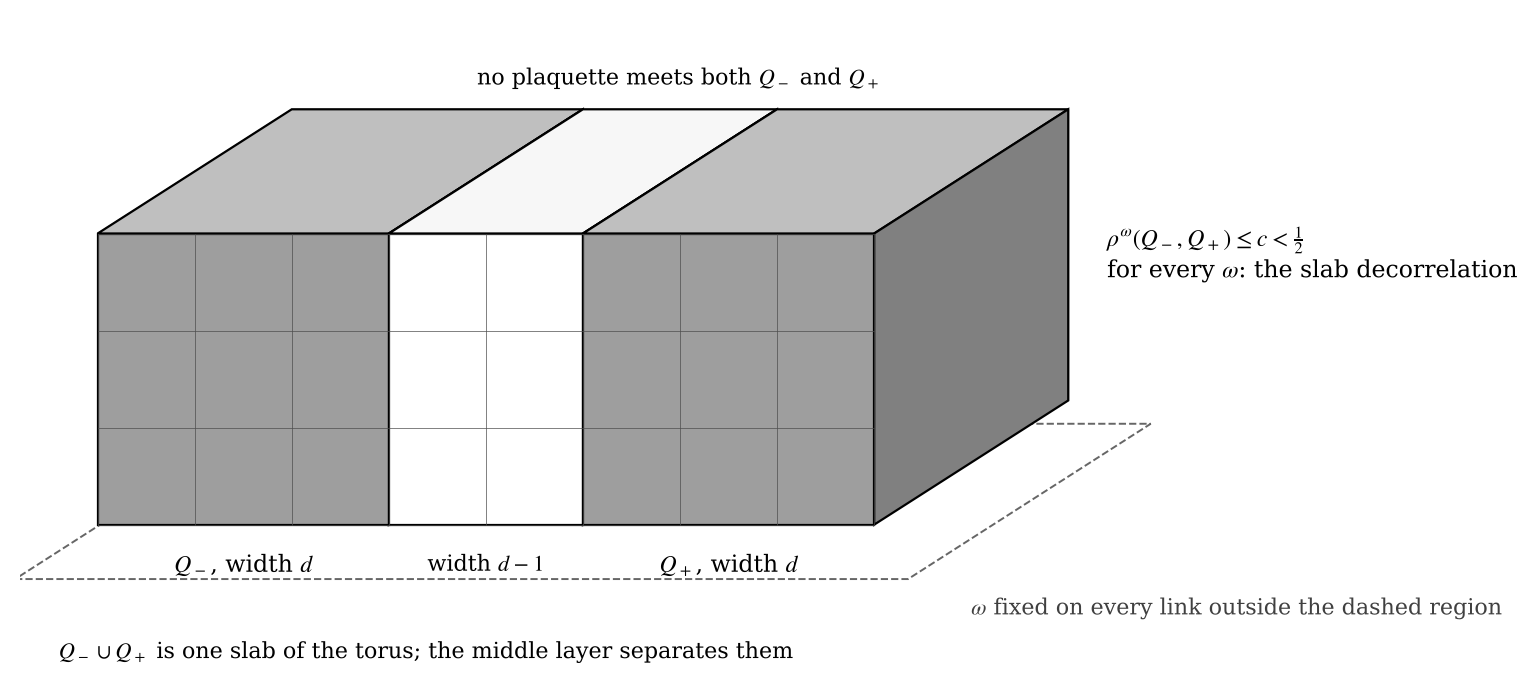
\includegraphics[width=\textwidth]{figures/fig_slab.png}
\caption{The splitting of Definition~\ref{def:M}: in the coordinate $i$ a box $Q$ of width $3d-1$ is cut into $Q_-$, $Q_0$, $Q_+$ of widths $d$, $d-1$, $d$; the middle is integrated out, the exterior configuration $\omega$ is fixed, and $\rho^\omega(Q_-,Q_+)$ is the maximal correlation of gauge-invariant observables of the two outer parts. No plaquette meets both $Q_-$ and $Q_+$, since the base points of the links of a plaquette differ by at most one in each coordinate and $d\ge2$.}
\label{fig:slab}
\end{figure}

The boxes of $(\mathrm M_{d,m}(c))$ are fat: all their widths are at least
$2d-1$. The restriction matters. In two dimensions the same condition for
boxes of width one in a transverse direction fails along the weak-coupling
tuning, through a broken global symmetry of a pinned strip, while the fat
form holds there (Theorem~\ref{thm:twod} and Proposition~\ref{prop:strip}
in Appendix~\ref{app:obstructions}). At $\varphi\equiv1$ the links are
independent under $\nu^\omega_Q$, so $\rho^\omega=0$ and both conditions hold
with $c=0$. Along the tuning, with $d\approx\ell/(2a)$, $(\mathrm
M_{d,m}(c))$ is a statement at the physical separation $(d-1)a\approx\ell/2$
in boxes of physical size at most about $m\ell/2$, uniform in the boundary
condition, and stated for all square-integrable gauge-invariant observables
of the two regions rather than for pairs of local ones.

\subsection{Two projections and a chain of projections}

\begin{lemma}\label{lem:friedrichs}
Let $P_1,P_2$ be orthogonal projections on a real Hilbert space $\mathcal K$,
$\mathcal N$ a closed subspace of $\operatorname{ran}P_1\cap
\operatorname{ran}P_2$, and suppose that $|\ip xy|\le c\|x\|\|y\|$ for all
$x\in\operatorname{ran}P_1\ominus\mathcal N$ and $y\in\operatorname{ran}P_2
\ominus\mathcal N$. Put $Q_k=I-P_k$ and $X=Q_1+Q_2$. Then $X^2\ge(1-c)X$,
that is, $Q_1Q_2+Q_2Q_1\ge-c(Q_1+Q_2)$.
\end{lemma}

\begin{proof}
For $n\in\mathcal N$, $P_kn=n$, so $Xn=0$; as $X$ is self-adjoint it also
preserves $\mathcal N^\perp$. Let $g\in\mathcal N^\perp$. Then $P_kg\perp
\mathcal N$, since $\ip{P_kg}n=\ip g{P_kn}=\ip gn=0$, so with $p=\|P_1g\|$
and $q=\|P_2g\|$, $|\ip{P_1g}{P_2g}|\le cpq$. Put $s=\ip g{(P_1+P_2)g}=
p^2+q^2$. Then $\|(P_1+P_2)g\|^2=p^2+q^2+2\ip{P_1g}{P_2g}\le(1+c)(p^2+q^2)$
and $s\le\|g\|\|(P_1+P_2)g\|\le\|g\|((1+c)s)^{1/2}$, so $s\le(1+c)\|g\|^2$
and $\ip g{Xg}=2\|g\|^2-s\ge(1-c)\|g\|^2$. So $X=0$ on $\mathcal N$, and on
$\mathcal N^\perp$ the operator $X-(1-c)$ is nonnegative and commutes with
$X\ge0$; hence $X^2-(1-c)X=X^{1/2}(X-(1-c))X^{1/2}\ge0$ there. Finally
$X^2-X=Q_1Q_2+Q_2Q_1$.
\end{proof}

The angle between $\operatorname{ran}P_1\ominus\mathcal N$ and
$\operatorname{ran}P_2\ominus\mathcal N$ is the Friedrichs angle of the two
ranges, and the lemma is a form of the classical relation between that angle
and the rate of the alternating projections~\cite{Deu01}.

\begin{lemma}\label{lem:chain}
Let $Q_0,\dots,Q_M$ be orthogonal projections on a real Hilbert space
$\mathcal K$ with $Q_tQ_{t'}=Q_{t'}Q_t$ whenever $|t-t'|\ge2$ and
$Q_tQ_{t+1}+Q_{t+1}Q_t\ge-c(Q_t+Q_{t+1})$ for $0\le t<M$, with $0\le c<
\frac12$. Then $H=\sum_tQ_t$ satisfies $H^2\ge(1-2c)H$, and $\ip g{Hg}\ge
(1-2c)\|g\|^2$ for every $g\perp\ker H$.
\end{lemma}

\begin{proof}
$H^2=\sum_tQ_t+\sum_{t<M}(Q_tQ_{t+1}+Q_{t+1}Q_t)+\sum Q_tQ_{t'}$, the last
sum over the ordered pairs with $|t-t'|\ge2$. Each such $Q_tQ_{t'}$ is a
product of commuting projections, hence a projection and nonnegative. The
middle sum is at least $-c\sum_{t<M}(Q_t+Q_{t+1})\ge-2cH$. So $H^2-(1-2c)H
\ge0$, and by the spectral theorem the spectrum of the nonnegative operator
$H$ lies in $\{0\}\cup[1-2c,\infty)$, which gives the second claim.
\end{proof}

\begin{lemma}\label{lem:constant}
Let $Q$ be a box, $\omega$ an exterior configuration, and $R_0,\dots,R_M$
subsets of $V(Q)$ with union $V(Q)$. If $F\in L^2(\nu^\omega_Q)$ is, for every
$t$, almost surely equal to a $\sigma(\sigma_{V(Q)\setminus
R_t})$-measurable function, then $F$ is almost surely constant.
\end{lemma}

\begin{proof}
The density of $\nu=\nu^\omega_Q$ with respect to $\lambda$ is bounded above
and below by positive constants, so $L^2(\nu)=L^2(\lambda)$ with the same
null sets. Let $\Lambda_t$ be the conditional expectation under $\lambda$
given $\sigma_{V(Q)\setminus R_t}$, which integrates out $\sigma_{R_t}$. By
hypothesis $F=F_t$ almost surely with $F_t$ a function of
$\sigma_{V(Q)\setminus R_t}$, so $\Lambda_tF=F_t=F$. By Fubini's theorem
$\Lambda_0\cdots\Lambda_M$ integrates out all of $\bigcup_tR_t=V(Q)$, so
$F=\Lambda_0\cdots\Lambda_MF$ is constant.
\end{proof}

\subsection{One direction}

Fix a box $R=\prod_iI_i$ and a coordinate $i$ with $I_i=[\alpha,\alpha+
(M+2)d-1)$ for an integer $M\ge0$. For $0\le t\le M$ let $R_t$ be the box
obtained from $R$ by replacing $I_i$ with $\alpha+dt+[0,2d-1)$, and for
$t<M$ let $Q_t$ be the box obtained by replacing $I_i$ with $\alpha+dt+
[0,3d-1)$, split into $Q_t^-$, $Q_t^0$, $Q_t^+$ by $\alpha+dt+[0,d)$,
$\alpha+dt+[d,2d-1)$ and $\alpha+dt+[2d-1,3d-1)$. Then
\begin{equation}\label{eq:slabs}
V(Q_t)=V(R_t)\cup V(R_{t+1}),\quad V(Q_t^-)=V(R_t)\setminus V(R_{t+1}),
\quad V(Q_t^+)=V(R_{t+1})\setminus V(R_t),
\end{equation}
and $\bigcup_tV(R_t)=V(R)$, since the intervals $\alpha+dt+[0,2d-1)$ cover
$I_i$.

\begin{proposition}[one direction]\label{prop:slab}
In this setting let $\omega$ be an exterior configuration of $R$,
$\nu=\nu^\omega_R$, $P_t=E_{V(R_t)}$, and suppose that $\rho^{\omega'}(Q^-_t,
Q^+_t)\le c<\frac12$ for every $t<M$ and every exterior configuration
$\omega'$ of $Q_t$. Then every $F\in\mathcal A^\omega_R$ satisfies
\[
(1-2c)\Var_\nu(F)\le\sum_{t=0}^M\nu\bigl((F-P_tF)^2\bigr).
\]
\end{proposition}

\begin{proof}
For $M=0$, $P_0F=\nu(F)$ and the claim is trivial; let $M\ge1$. Put
$\mathcal K=\mathcal A^\omega_R$. By Lemma~\ref{lem:boxinv}(iii) each $P_t$
preserves $\mathcal K$ and restricts to an orthogonal projection of
$\mathcal K$; let $Q_t=I-P_t$ on $\mathcal K$.

\emph{Non-adjacent moves commute.} Let $t'\ge t+2$. The base points of the
links of $V(R_t)$ have $i$-th coordinate at most $\alpha+dt+2d-2$ and those
of $V(R_{t'})$ at least $\alpha+dt+2d$, so no plaquette meets both sets.
Given $\sigma$ off $V(R_t)\cup V(R_{t'})$, the conditional density of
$(\sigma_{V(R_t)},\sigma_{V(R_{t'})})$ is a product of factors each of which
involves the links of only one of the two sets. So they are conditionally
independent, and $P_tP_{t'}F$ and $P_{t'}P_tF$ are both the integral of $F$
against the product of the two conditional laws. Hence $P_tP_{t'}=
P_{t'}P_t$, and the $Q_t$ commute.

\emph{Adjacent moves.} Fix $t<M$ and write $a=V(Q_t^-)$, $b=V(Q_t^0)$,
$c'=V(Q_t^+)$, $e=V(R)\setminus V(Q_t)$. By~\eqref{eq:slabs},
$V(R)\setminus V(R_t)=c'\cup e$ and $V(R)\setminus V(R_{t+1})=a\cup e$, so
the ranges of $P_t$ and of $P_{t+1}$ in $\mathcal K$ are the elements of
$\mathcal K$ measurable with respect to $(\sigma_{c'},\sigma_e)$ and to
$(\sigma_a,\sigma_e)$. Let $\mathcal N$ be the elements of $\mathcal K$
measurable with respect to $\sigma_e$, a closed subspace of both ranges. We
check the hypothesis of Lemma~\ref{lem:friedrichs}. Let $x$ and $y$ be in
the ranges of $P_t$ and $P_{t+1}$ and orthogonal to $\mathcal N$. The
conditional expectation $E_e$ given $\sigma_e$ is $E_{V(Q_t)}$, which
preserves $\mathcal K$, so $E_ex\in\mathcal N$ and $\|E_ex\|^2=\ip x{E_ex}=0$;
likewise $E_ey=0$. By Lemma~\ref{lem:boxinv}(iii) for the box $R$ take
versions $x=\tilde x(\sigma_{c'},\sigma_e)$ and $y=\tilde y(\sigma_a,\sigma_e)$
invariant at every point under $\mathcal G_R$. Every vertex interior to $Q_t$
is interior to $R$, so $\mathcal G_{Q_t}\subset\mathcal G_R$, and
$\mathcal G_{Q_t}$ fixes $\sigma_e$. Hence for each $\eta\in G^e$ the
functions $X_\eta=\tilde x(\cdot,\eta)$ of $\sigma_{V(Q^+_t)}$ and $Y_\eta=
\tilde y(\cdot,\eta)$ of $\sigma_{V(Q^-_t)}$ are invariant under
$\mathcal G_{Q_t}$ at every point. The conditional law of $\sigma_{V(Q_t)}$
given $\sigma_e=\eta$ is $\nu_\eta=\nu^{(\eta,\omega)}_{Q_t}$, so for almost
every $\eta$, $X_\eta,Y_\eta\in L^2(\nu_\eta)$, $\nu_\eta(X_\eta)=(E_ex)(\eta)
=0$, $\nu_\eta(Y_\eta)=0$, and by the hypothesis with $\omega'=(\eta,\omega)$,
\[
|\nu_\eta(X_\eta Y_\eta)|\le c\,\nu_\eta(X_\eta^2)^{1/2}\nu_\eta(Y_\eta^2)^{1/2}.
\]
Integrating over $\eta$ and using the Cauchy--Schwarz inequality,
$|\ip xy|\le c\|x\|\|y\|$, and Lemma~\ref{lem:friedrichs} gives
$Q_tQ_{t+1}+Q_{t+1}Q_t\ge-c(Q_t+Q_{t+1})$ on $\mathcal K$.

\emph{Conclusion.} Lemma~\ref{lem:chain} applies. If $Hg=0$ for $g\in
\mathcal K$, then $\sum_t\|Q_tg\|^2=\ip g{Hg}=0$, so $g=P_tg$ for all $t$ and
$g$ is constant by Lemma~\ref{lem:constant}. For $F\in\mathcal K$ the
function $g=F-\nu(F)$ is orthogonal to the constants, hence to $\ker H$, and
$\ip g{Hg}=\sum_t\nu((F-P_tF)^2)$.
\end{proof}

\subsection{The patch gap and the cube condition}

For $d\ge2$, $m\ge4$ and $r\in\Z^4$ let $\Pi=r+[0,md-1)^4$, the box of
base points of a patch, and for $j\in[0,m-2]^4$ let $B_j=V(r+dj+
[0,2d-1)^4)$, as in Appendix~\ref{app:finite}. For an exterior
configuration $\omega$ of $\Pi$ write $\nu=\nu^\omega_\Pi$ and $P_j=E_{B_j}$.

\begin{theorem}[patch gap from slab decorrelation]\label{thm:patch}
Let $d\ge2$, $m\ge4$, $0\le c<\frac12$, and assume $(\mathrm M_{d,m}(c))$.
Then for every $r$, every $\omega$ and every $F\in\mathcal A^\omega_\Pi$,
\[
(1-2c)^4\Var_\nu(F)\le\sum_{j\in[0,m-2]^4}\nu\bigl((F-P_jF)^2\bigr).
\]
\end{theorem}

\begin{proof}
For $0\le k\le4$ and $\tau\in[0,m-2]^k$ let $R^{(k)}_\tau=r+\prod_{i\le k}
(d\tau_i+[0,2d-1))\times[0,md-1)^{4-k}$ and $P^{(k)}_\tau=
E_{V(R^{(k)}_\tau)}$, under $\nu$. We prove by induction on $k$ that
\[
(1-2c)^k\Var_\nu(F)\le\sum_{\tau\in[0,m-2]^k}\nu\bigl((F-P^{(k)}_\tau F)^2
\bigr)\qquad(F\in\mathcal A^\omega_\Pi).
\]
For $k=0$, $R^{(0)}=\Pi$ and $P^{(0)}F=\nu(F)$. Let $k<4$, fix $\tau$, write
$R=R^{(k)}_\tau$, and split $\sigma=(\sigma',\omega')$ with $\sigma'=
\sigma_{V(R)}$ and $\omega'=\sigma_{V(\Pi)\setminus V(R)}$. Take $F$
invariant at every point under $\mathcal G_\Pi$ (Lemma~\ref{lem:boxinv}(iii)).
Since $\mathcal G_R\subset\mathcal G_\Pi$ fixes $\omega'$, each
$F(\cdot,\omega')$ is invariant under $\mathcal G_R$. The conditional law of
$\sigma'$ given $\omega'$ is $\nu'=\nu^{(\omega',\omega)}_R$, so
\[
\nu\bigl((F-P^{(k)}_\tau F)^2\bigr)=\int\Var_{\nu'}\bigl(F(\cdot,\omega')
\bigr)\,d\nu(\omega').
\]
In the coordinate $k+1$ the box $R$ has width $md-1=((m-2)+2)d-1$. The
boxes $R_u$ and $Q_u$ of Proposition~\ref{prop:slab} built from $R$ with
$i=k+1$ and $M=m-2$ are $R_u=R^{(k+1)}_{(\tau,u)}$ and boxes whose widths are
$2d-1$ in the coordinates $\le k$, $3d-1$ in the coordinate $k+1$ and $md-1$
in the coordinates $>k+1$, split as in $(\mathrm M_{d,m}(c))$; all these
widths lie in $[2d-1,md-1]$. By Proposition~\ref{prop:slab}, for almost every
$\omega'$,
\[
(1-2c)\Var_{\nu'}(F(\cdot,\omega'))\le\sum_{u=0}^{m-2}\nu'\bigl((F(\cdot,
\omega')-P'_uF(\cdot,\omega'))^2\bigr),
\]
with $P'_u$ the conditional expectation under $\nu'$ given $\sigma'$ off
$V(R^{(k+1)}_{(\tau,u)})$. The conditional law of the links of that set given
the other links of $\Pi$ is the same under $\nu$ and under $\nu'$, both
having density proportional to $\prod_p\varphi(U_p)$ over the plaquettes
meeting it; so $P'_uF(\cdot,\omega')=(P^{(k+1)}_{(\tau,u)}F)(\cdot,\omega')$,
and integrating over $\omega'$ gives $\nu((F-P^{(k+1)}_{(\tau,u)}F)^2)$.
Multiplying the induction hypothesis by $1-2c$ and inserting these bounds
proves the case $k+1$. For $k=4$, $V(R^{(4)}_\tau)=B_\tau$.
\end{proof}

\begin{mainthm}[mass generation implies the cube condition]\label{thm:D}
Let $d\ge2$, $0\le c<\frac12$ and $m\ge4$ with $m-1\ge148/(1-2c)^4$, and
assume $(\mathrm M_{d,m}(c))$. Then for every even $L$ with $d\mid L$ and
$L\ge2md$ the measure $\mu_L$ with weight $\varphi$ satisfies
\[
\BP\Bigl(2d-1,\frac{(1-2c)^4}{32}\Bigr).
\]
Consequently, let $(\beta_k,a_k)$ be a tuning with $a_k\to0$ and Wilson
weights, and $d_k\ge2$ integers with $(2d_k-1)a_k\le\ell$. If
$(\mathrm M_{d_k,m}(c))$ holds for every $k$ with $c<\frac12$ and $m$ as
above independent of $k$, then statement (D) holds with $n_k=2d_k-1$ and
$\varpi=(1-2c)^4/32$, and every continuum limit as in Theorem~\ref{thm:B}
along the tori with $d_k\mid L$ satisfies
\[
\sigma(H)\subset\{0\}\cup\Bigl[\frac{(1-2c)^4}{1250\,e^2\ell},\infty\Bigr),
\]
with $0$ a simple eigenvalue; a nontrivial limit has a mass gap at least
this large.
\end{mainthm}

\begin{proof}
Theorem~\ref{thm:patch} says that the gauge-invariant patch gap of
Definition~\ref{def:patchgap} satisfies $\gamma_{d,m}\ge(1-2c)^4$, and
Theorem~\ref{thm:finite} with $\gamma=(1-2c)^4$ gives
$\BP(2d-1,(1-2c)^4/32)$. Along the tuning this holds on an infinite set of
even tori with $L\ge2(2d_k-1)+4$ for each $k$, with $(2d_k-1)a_k\le\ell$, and
Theorem~\ref{thm:B} gives the gap $16\varpi/(625e^2\ell)$ with
$\varpi=(1-2c)^4/32$.
\end{proof}

\begin{corollary}[cylinders and anisotropic tori]\label{cor:cylinders}
Under the hypotheses of Theorem~\ref{thm:D}, $\BP(2d-1,(1-2c)^4/32)$ holds
for the measure with weight $\varphi$ on every torus $\prod_{i=1}^4(\Z/L_i\Z)$
with $d\mid L_i$ and $L_i\ge2md$ for every $i$; in particular on every
cylinder $\Lambda_{L,M}=(\Z/L\Z)^3\times(\Z/M\Z)$ with $d\mid L$, $d\mid M$
and $L,M\ge2md$.
\end{corollary}

\begin{proof}
The side of the torus enters the proof of Theorem~\ref{thm:D} only through
Appendix~\ref{app:finite}, and there only coordinate by coordinate. With
$K_i=L_i/d\ge2m$ the coarse torus is $\prod_i(\Z/K_i\Z)$ and the blocks
$B_j$ are as before. Lemma~\ref{lem:fcommute}(ii) needs $K_i\ge4$ in the
coordinate $i$ in which $|v_i|\ge2$. In Lemma~\ref{lem:knabe}, two indices
$j$, $j+v$ lie in a common patch only if $|v_i|\le m-2$ for every $i$,
which uses $K_i\ge2m$ in each coordinate, and then for exactly $c_v=
\prod_i(p-|v_i|)$ patches; the rest of that proof is algebra in $p$ and
$\gamma$. The patch inequality of Theorem~\ref{thm:finite} needs the patch
and its exterior to be disjoint, that is $L_i\ge md+2$ in each coordinate;
the averaging over the shifts $a\in[0,d)^4$ and the bound $L_i\ge8d\ge2n+4$
are unchanged, and Theorem~\ref{thm:decay} is stated for such tori. Parity
of the sides is used nowhere.
\end{proof}

The patch gap obtained, $(1-2c)^4$, does not decay with $m$, whereas the
finite-size criterion needs only $148/(m-1)$; this slack is what allows a
large but fixed number $m$ of blocks per patch. The threshold $c<\frac12$
cannot be raised for this argument: for the massless Gaussian chain every
adjacent pair of moves has maximal correlation exactly $\frac12$, the
non-adjacent moves commute, and the gap of the slab dynamics tends to zero
(Proposition~\ref{prop:gausschain}).

\subsection{Decay of correlations under every boundary condition}

\begin{lemma}\label{lem:boxmarkov}
Let $Q$ be a box, $\omega$ an exterior configuration, $i$ a coordinate, and
$Y_0,\dots,Y_K$ the sets $V(Q\cap\{x_i\in J_k\})$ for consecutive nonempty
integer intervals $J_0<J_1<\dots<J_K$ whose union is the $i$-th side of $Q$.
Under $\nu^\omega_Q$, for each $k$, the families $(\sigma_{Y_l})_{l<k}$ and
$(\sigma_{Y_l})_{l>k}$ are conditionally independent given $\sigma_{Y_k}$.
\end{lemma}

\begin{proof}
The links in $V(Q)$ of a plaquette are based at points whose $i$-th
coordinates take at most two consecutive values, so they lie in one $Y_l$ or
in two consecutive ones. Grouping the factors of the density by the least
$l$ met, the density of $\nu^\omega_Q$ with respect to $\lambda$ is
$\prod_l\psi_l(\sigma_{Y_l},\sigma_{Y_{l+1}})$, with $\psi_K$ a function of
$\sigma_{Y_K}$, which gives the conditional independence.
\end{proof}

\begin{proposition}\label{prop:alldecay}
Assume $(\mathrm M^*_w(c))$ with $w\ge1$ and $0\le c\le1$. Let $Q$ be a box,
$\omega$ an exterior configuration, $\nu=\nu^\omega_Q$, $i$ a coordinate,
$s\in\Z$, $r\ge1$, and let $f,g\in\mathcal A^\omega_Q$ be measurable with
respect to $\sigma_{V(Q\cap\{x_i\le s\})}$ and $\sigma_{V(Q\cap\{x_i\ge
s+r\})}$. Then
\[
|\Cov_\nu(f,g)|\le c^{\lfloor r/(w+1)\rfloor}\|f-\nu(f)\|\,\|g-\nu(g)\|.
\]
\end{proposition}

\begin{proof}
If one of the two parts of $Q$ is empty, $f$ or $g$ is constant and the
covariance vanishes. Otherwise the $i$-th side of $Q$ contains $[s,s+r]$.
Let $J=\lfloor r/(w+1)\rfloor$; for $J=0$ the claim is the Cauchy--Schwarz
inequality. Let $J\ge1$ and split the $i$-th side into consecutive
intervals: $T_0$, the values $\le s$; for $1\le k\le J$, $M_k=[s+(k-1)(w+1)+
1,\,s+(k-1)(w+1)+w]$; for $1\le k\le J-1$, $T_k=\{s+k(w+1)\}$; and $T_J$, the
values $\ge s+J(w+1)$, which contain the values $\ge s+r$. Use the same
letters for the corresponding sets of links. By Lemma~\ref{lem:boxmarkov}
the sequence $T_0,M_1,T_1,\dots,M_J,T_J$ is Markov, and by
Lemma~\ref{lem:boxinv} the conditional expectations given $\sigma_{T_k}$
preserve $\mathcal A^\omega_Q$.

For $1\le k\le J$ let $u\in\mathcal A^\omega_Q$ be a centred function of
$\sigma_{T_{k-1}}$ and $v=E[u\mid\sigma_{T_k}]$, which is centred and lies
in $\mathcal A^\omega_Q$. The box $Q$ splits in the coordinate $i$ into the
values $\le s+(k-1)(w+1)$, the middle $M_k$ of width $w$, and the values
$\ge s+k(w+1)$; $u$ is a function of the first part and $v$ of the last, so
by $(\mathrm M^*_w(c))$, $\|v\|^2=\nu(uv)\le c\|u\|\|v\|$, that is,
$\|v\|\le c\|u\|$. Let $f_0=f-\nu(f)$ and $u_k=E[f_0\mid\sigma_{T_k}]$. By
the Markov property $u_k=E[u_{k-1}\mid\sigma_{T_k}]$, so $\|u_k\|\le
c\|u_{k-1}\|$ and $\|u_J\|\le c^J\|f_0\|$. As $g$ is
$\sigma_{T_J}$-measurable, $\Cov_\nu(f,g)=\nu(u_J(g-\nu(g)))$, and the
Cauchy--Schwarz inequality gives the claim.
\end{proof}

So $(\mathrm M^*_{d-1}(c))$ with $c<1$, which contains $(\mathrm
M_{d,m}(c))$ for every $m$, gives exponential decay of the covariances of
gauge-invariant observables of a box, uniformly in the box and in the
boundary condition, at rate $\log(1/c)/d$ per lattice spacing, that is, of
order $\log(1/c)/\ell$ in physical units along the tuning. This is close to
the decay hypothesis of Chatterjee~\cite[Def.~2.3]{Cha21}, under which an
area law for Wilson loops follows; there the observables are local
functions of a cube with prescribed boundary, and the geometries differ, so
neither condition is claimed to imply the other. The converse direction is
the weak point of any pairwise form: a bound $K_1e^{-K_2r}$ for pairs of
local functions, summed over the pairs of two slabs of transverse size
$(md)^3$, bounds $\rho^\omega$ only up to a factor of order $(md)^6$, which
is not uniform in the lattice spacing.

\subsection{The hypothesis reduced to one layer, and its vacuum form}
\label{ssec:layers}

Two reductions locate what $(\mathrm M_{d,m}(c))$ asks beyond a mass gap.
The first says that the maximal correlation of the two outer parts of a box
is the maximal correlation of their two inner layers, and that it is
multiplicative over the layers in between; the second computes the same
quantity, with the Dirichlet law of a box replaced by the vacuum of a
cylinder, in terms of the spectral gap of the transfer matrix. Together they
show that the content of the hypothesis is the uniformity in the boundary
condition, and nothing else.

Let $Q$ be a box, $i$ a coordinate in which $Q$ has width $s$, and for
$0\le j<s$ let $Y_j$ be the set of links of $V(Q)$ whose base points have
$i$-th coordinate equal to the $j$-th value of the $i$-th side of $Q$: the
\emph{layers} of $Q$ in the coordinate $i$. For an exterior configuration
$\omega$, $\nu=\nu^\omega_Q$, and two layers $Y,Y'$ put
\[
\rho^\omega(Y,Y')=\sup|\nu(XX')|,
\]
the supremum over $X,X'\in\mathcal A^\omega_Q$ measurable with respect to
$\sigma_Y$ and $\sigma_{Y'}$ respectively, with $\nu(X)=\nu(X')=0$ and
$\nu(X^2)=\nu(X'^2)=1$. This is the maximal correlation of the gauge-invariant
observables of the two layers; it is defined also for adjacent layers,
which share plaquettes.

\begin{lemma}[layers]\label{lem:layers}
Let $Q$, $i$, $\omega$ and the layers $Y_0,\dots,Y_{s-1}$ be as above.
\begin{enumerate}[label=\textup{(\roman*)},leftmargin=*]
\item For a splitting $Q=Q_-\cup Q_0\cup Q_+$ in the coordinate $i$ as in
Definition~\textup{\ref{def:rho}}, with $Q_-$ and $Q_0$ of widths $s_-$ and
$s_0$,
\[
\rho^\omega(Q_-,Q_+)=\rho^\omega(Y_{s_--1},Y_{s_-+s_0}).
\]
\item For $0\le j<j+r<s$,
\[
\rho^\omega(Y_j,Y_{j+r})\le\prod_{l=j}^{j+r-1}\rho^\omega(Y_l,Y_{l+1}).
\]
\end{enumerate}
In particular, if $\rho^\omega(Y_l,Y_{l+1})\le\theta$ for every box $Q$ all
of whose widths lie in $[2d-1,md-1]$, every coordinate, every $l$ and every
$\omega$, then $(\mathrm M_{d,m}(\theta^d))$ holds.
\end{lemma}

\begin{proof}
Write $k=s_--1$ and $k'=s_-+s_0$, so that $V(Q_-)=Y_0\cup\dots\cup Y_k$ and
$V(Q_+)=Y_{k'}\cup\dots\cup Y_{s-1}$. By Lemma~\ref{lem:boxmarkov}, applied
to the layers themselves, the families $(\sigma_{Y_l})_{l<k}$ and
$(\sigma_{Y_l})_{l>k}$ are conditionally independent given $\sigma_{Y_k}$.
Hence for an integrable $X$ measurable with respect to
$\sigma(\sigma_{Y_l}:l\le k)$,
\begin{equation}\label{eq:layermarkov}
E[X\mid\sigma_{Y_l}:l\ge k]=E[X\mid\sigma_{Y_k}],
\end{equation}
and symmetrically with the two sides exchanged, at every layer $k$.

(i) The inequality $\ge$ holds because a pair admissible for the right side
is admissible for the left. For $\le$ let $X,X'$ be admissible for
$\rho^\omega(Q_-,Q_+)$ and put $\tilde X=E[X\mid\sigma_{Y_k}]$, $\tilde
X'=E[X'\mid\sigma_{Y_{k'}}]$. Both are centred, of norm at most $1$, and lie
in $\mathcal A^\omega_Q$ by Lemma~\ref{lem:boxinv}(iii), since each is a
conditional expectation given the links of a subset of $V(Q)$. As $X'$ is
measurable with respect to $\sigma(\sigma_{Y_l}:l\ge k)$,
\eqref{eq:layermarkov} gives $\nu(XX')=\nu(\tilde XX')$, and as $\tilde X$ is
measurable with respect to $\sigma(\sigma_{Y_l}:l\le k')$, the symmetric
identity at the layer $k'$ gives $\nu(\tilde XX')=\nu(\tilde X\tilde X')$. So
$|\nu(XX')|\le\rho^\omega(Y_k,Y_{k'})\|\tilde X\|\,\|\tilde X'\|\le
\rho^\omega(Y_k,Y_{k'})$.

(ii) It suffices to treat $r\ge2$ and to show $\rho^\omega(Y_j,Y_{j+r})\le
\rho^\omega(Y_j,Y_l)\,\rho^\omega(Y_l,Y_{j+r})$ for $j<l<j+r$; the product
follows by induction on $r$. Let $X$, $X'$ be admissible for
$\rho^\omega(Y_j,Y_{j+r})$ and $Z=E[X'\mid\sigma_{Y_l}]$, which is centred
and lies in $\mathcal A^\omega_Q$. By~\eqref{eq:layermarkov} at the layer $l$,
$\nu(XX')=\nu(XZ)$ and $\nu(X'Z)=\nu(Z^2)=\|Z\|^2$. The first identity gives
$|\nu(XX')|\le\rho^\omega(Y_j,Y_l)\|Z\|$, the second $\|Z\|^2\le
\rho^\omega(Y_l,Y_{j+r})\|Z\|$, that is, $\|Z\|\le\rho^\omega(Y_l,Y_{j+r})$,
and the claim follows.

For the last assertion, in the splitting of Definition~\ref{def:M} the two
layers of (i) are $Y_{d-1}$ and $Y_{2d-1}$, at distance $d$, and (ii) gives
$\rho^\omega(Q_-,Q_+)\le\theta^d$.
\end{proof}

So the hypothesis is a bound, uniform in the boundary condition, on the
second singular value of the $d$-step transfer operator of the box between
two of its layers, on gauge-invariant functions; and it follows from a bound
$\theta$ on the one-step operator between adjacent layers whenever
$\theta^d\le c$. In the vacuum of a cylinder the corresponding quantity is
known exactly.

\begin{proposition}[the vacuum form of the hypothesis]\label{prop:vacuumlayers}
Let $L\ge1$, let $\mathbb T$, $\lambda_0$, $\Omega_0$ and $\mu^0_L$ be as in
Lemma~\textup{\ref{lem:transfer}}, and let $\lambda_0\rho_1$ be the largest
modulus of an eigenvalue $\lambda\ne\lambda_0$ of $\mathbb T$, so that
$0\le\rho_1<1$. For $s\ge1$ let $\rho^{\mathrm{vac}}_L(s)$ be the supremum
of $\mu^0_L(F\,\tau_sH)$ over the real bounded gauge-invariant functions
$F,H$ of the slice $E_0$ with $\mu^0_L(F)=\mu^0_L(H)=0$ and $\mu^0_L(F^2)=
\mu^0_L(H^2)=1$. Then
\[
\rho^{\mathrm{vac}}_L(s)=\rho_1^{\,s}\qquad(s\ge1).
\]
\end{proposition}

\begin{proof}
By Lemma~\ref{lem:transfer}(v) with $w=w'=0$, and $\vartheta\bar F=F$ for a
real function of the slice $E_0$, $\mu^0_L(F\,\tau_sH)=\ip{F\Omega_0}
{\mathbb R^sH\Omega_0}$, $\mu^0_L(F)=\ip{\Omega_0}{F\Omega_0}$ and
$\mu^0_L(F^2)=\|F\Omega_0\|^2$, with $\mathbb R=\mathbb T/\lambda_0$ and
$\|\Omega_0\|=1$. Let $\mathcal K^G$ be the closed subspace of gauge-invariant
elements of $\mathcal K$ and $\mathcal K^G_0=\mathcal K^G\ominus\Omega_0$;
$\Omega_0\in\mathcal K^G$ by Lemma~\ref{lem:transfer}(i). The map $F\mapsto
u=F\Omega_0$ sends the admissible $F$ to unit vectors of $\mathcal K^G_0$,
since the product of two gauge-invariant functions is gauge invariant. Its
image is dense in the unit sphere of $\mathcal K^G_0$: given a unit
$u\in\mathcal K^G_0$, the function $u/\Omega_0$ is gauge invariant,
measurable, and in $L^2(\Omega_0^2\lambda)$; its truncations $F_n=
(u/\Omega_0)\mathbf 1\{|u/\Omega_0|\le n\}$ are bounded and gauge invariant,
$F_n\Omega_0\to u$ in $\mathcal K$ by dominated convergence, and $F_n'=F_n-
\mu^0_L(F_n)$ is admissible after normalisation, with $F_n'\Omega_0\to u-
\ip{\Omega_0}{u}\Omega_0=u$. Hence
\[
\rho^{\mathrm{vac}}_L(s)=\sup\{\ip u{\mathbb R^sv}:u,v\in\mathcal K^G_0,\
\|u\|=\|v\|=1\}=\|\mathbb R^s|_{\mathcal K^G_0}\|,
\]
the supremum of a continuous function over a dense subset being its
supremum over the set. By the proof of Lemma~\ref{lem:transfer}(i),
$\mathbb T$ maps $\mathcal K$ into $\mathcal K^G$, and it is self-adjoint and
maps $\Omega_0$ to $\lambda_0\Omega_0$; so $\mathbb R$ maps $\mathcal K^G_0$
into itself, and its restriction is compact and self-adjoint. The nonzero
eigenvalues of that restriction are the numbers $\lambda/\lambda_0$ for the
eigenvalues $\lambda\ne\lambda_0$ of $\mathbb T$: every eigenvector with
nonzero eigenvalue is gauge invariant by Lemma~\ref{lem:transfer}(i), and
those with $\lambda\ne\lambda_0$ are orthogonal to $\Omega_0$. The norm of
the $s$-th power of a compact self-adjoint operator is the $s$-th power of
its largest eigenvalue modulus, which is $\rho_1$.
\end{proof}

Under the vacuum law of the cylinder the maximal correlation of the
gauge-invariant observables of two slices at distance $s$ is thus
$e^{-m_{\mathrm{lat}}s}$ with $m_{\mathrm{lat}}=-\log\rho_1$ the lattice
gap, with no constant in front; a physical gap $m$ gives $\rho^{\mathrm
{vac}}_L(d)\le e^{-mda}<\frac12$ as soon as $da>(\log2)/m$, and for
adjacent slices it gives exactly $\rho_1$, so that the product of
Lemma~\ref{lem:layers}(ii) is an equality in the vacuum.\footnote{The
two statements concern different laws. Proposition~\ref{prop:vacuumlayers}
is about the state $\mu^0_L$ of the infinite cylinder, in which the slices
outside $[0,s]$ are integrated against the vacuum; $(\mathrm M_{d,m}(c))$ is
about the law $\nu^\omega_Q$ of a box of bounded physical size whose
exterior is held fixed at an arbitrary $\omega$. Along the tuning of
Section~\ref{sec:weak} the box has physical side between $\ell$ and $m\ell/2$,
and $d$ layers correspond to the physical distance $\ell/2$, so the vacuum
form of the bound $c<\frac12$ reads $m\ell>2\log2$.} Theorem~\ref{thm:D}
with Corollary~\ref{cor:cylinders} and Proposition~\ref{prop:cylindergap}
goes from $(\mathrm M_{d,m}(c))$ to a gap; the proposition goes from a gap
back to the vacuum form of $(\mathrm M_{d,m}(c))$ without loss. The two do
not close into a proof because the hypothesis is stated under every exterior
configuration, and the vacuum is one law among them: what is missing is
precisely that the second singular value of the one-layer transfer operator
of a box of physical size $\ell$ stays below $c^{1/d}$ for every boundary
condition, uniformly along the tuning. Appendix~\ref{app:obstructions} shows
in two dimensions that a twisted boundary condition can drive the
correlation of a thin strip to $1$, so the uniformity is not a formality;
in four dimensions it is the statement that no boundary condition at the
distance $\ell/2$ orders the gauge-invariant observables of the box, and it
is here that the non-abelian input must enter.

The uniformity cannot fail at any fixed box: in the class of weights
considered here no boundary condition locks a layer, so the question is
asymptotic, in the size of the box at fixed coupling or along the tuning
in boxes of fixed physical size.

\begin{proposition}[no boundary condition locks a layer]\label{prop:nolock}
Let $G$ be compact, $\varphi$ a positive continuous class function, $Q$ a box
and $Y,Y'\subset V(Q)$ disjoint. Then the supremum over all exterior
configurations $\omega$ and all centred unit $X\in L^2(\nu^\omega_Q)$
measurable with respect to $\sigma_Y$ and $X'$ measurable with respect to
$\sigma_{Y'}$ of $|\nu^\omega_Q(XX')|$ is less than $1$. In particular
$\sup_\omega\rho^\omega(Y_k,Y_{k+1})<1$ and $\sup_\omega\rho^\omega(Q_-,Q_+)<1$
for every box and splitting, and $(\mathrm M_{d,m}(c))$ holds for some
$c<1$ for every $d$, $m$ and $\varphi$.
\end{proposition}

\begin{proof}
The density $f_\omega$ of $\nu^\omega_Q$ with respect to the Haar measure
$\lambda$ of $G^{V(Q)}$ depends on finitely many exterior links, those of
the plaquettes meeting $V(Q)$, so $\omega$ ranges over a compact set
$\Omega$, $\omega\mapsto f_\omega$ is continuous from $\Omega$ to
$C(G^{V(Q)})$, and $m_0\le f_\omega\le M_0$ with $m_0=(\min\varphi/
\max\varphi)^P>0$, $P$ the number of those plaquettes, and $M_0=1/m_0$. Let
$k_\omega(y,y')$ be the joint density of $(\sigma_Y,\sigma_{Y'})$ with
respect to $\lambda_Y\otimes\lambda_{Y'}$ and $k^{Y'}_\omega$ the marginal
density of $\sigma_{Y'}$, integrals of $f_\omega$ over the other links,
hence continuous in $(\omega,y,y')$ and between $m_0$ and $M_0$. The
conditional expectation given $\sigma_{Y'}$ of a function $g$ of $\sigma_Y$
is $(B_\omega g)(y')=\int g(y)k_\omega(y,y')\,d\lambda_Y(y)/k^{Y'}_\omega(y')$,
an operator from $L^2(\lambda_Y)$ to $L^2(\lambda_{Y'})$ with a continuous
kernel depending continuously on $\omega$ in the uniform norm; so each
$B_\omega$ is Hilbert--Schmidt, hence compact, and $\omega\mapsto B_\omega$
is continuous in the Hilbert--Schmidt norm.

Suppose the claim fails: there are $\omega_n\in\Omega$ and admissible
$X_n,X'_n$ with $\nu^{\omega_n}(X_nX'_n)\to1$. Pass to a subsequence with
$\omega_n\to\omega$. In $L^2(\nu^{\omega_n})$, $\|X_n-X'_n\|^2=2-2\nu^{\omega_n}
(X_nX'_n)\to0$, and since the densities lie in $[m_0,M_0]$ the $X_n,X'_n$ are
bounded in $L^2(\lambda)$ with $\|X_n-X'_n\|_{L^2(\lambda)}\to0$. Pass to a
further subsequence with $X_n\rightharpoonup X$ and $X'_n\rightharpoonup X'$
weakly in $L^2(\lambda)$; $X$ is a function of $\sigma_Y$, $X'$ one of
$\sigma_{Y'}$, and $X=X'$ almost everywhere. Under the product measure
$\lambda$ a function of $\sigma_Y$ that agrees almost everywhere with a
function of the disjoint variables $\sigma_{Y'}$ is almost everywhere a
constant $\kappa$, and $0=\nu^{\omega_n}(X_n)=\int X_nf_{\omega_n}\,d\lambda\to
\int Xf_\omega\,d\lambda=\kappa$ by the weak convergence of $X_n$ and the
uniform convergence of $f_{\omega_n}$. So $X=0$. Now
$\nu^{\omega_n}(X_nX'_n)=\nu^{\omega_n}\bigl((B_{\omega_n}X_n)X'_n\bigr)\le
\|B_{\omega_n}X_n\|_{L^2(\nu^{\omega_n})}\le M_0^{1/2}\|B_{\omega_n}X_n\|_{L^2
(\lambda)}$, and $B_{\omega_n}X_n=B_\omega X_n+(B_{\omega_n}-B_\omega)X_n\to
B_\omega X=0$ strongly, because $B_\omega$ is compact and $\|B_{\omega_n}-
B_\omega\|\to0$. This contradicts $\nu^{\omega_n}(X_nX'_n)\to1$.
\end{proof}

A model in which a boundary condition locks a layer must therefore have a
weight with zeros, outside the class of Lemma~\ref{lem:transfer}; and the
two-dimensional strip of Appendix~\ref{app:obstructions} drives the
correlation to $1$ only in the limit along the tuning.

The supremum in Proposition~\ref{prop:nolock} is attained, because the
slab correlation depends continuously on the boundary condition.

\begin{lemma}[continuity in the boundary condition]\label{lem:rhocont}
Fix a box $Q$ and a splitting $Q_\pm$. The map $\omega\mapsto\rho^\omega
(Q_-,Q_+)$ is uniformly continuous on the compact space $\Omega$ of the
exterior configurations that enter $\nu^\omega_Q$. Consequently $\sup_\omega
\rho^\omega(Q_-,Q_+)$ is attained, it equals the supremum over any dense set
of $\omega$, and $\{\omega:\rho^\omega(Q_-,Q_+)>c\}$ is open for every $c$.
\end{lemma}

\begin{proof}
Write $\sigma=(x,z,y)$ with $x=\sigma_{V(Q_-)}$ and $y=\sigma_{V(Q_+)}$, let
$f^\omega$ be the density of $\nu^\omega_Q$ with respect to Haar measure,
$j^\omega(x,y)=\int f^\omega\,dz$ the joint density of $(x,y)$ with marginals
$j^\omega_\pm$, and $k^\omega=j^\omega/(j^\omega_-\otimes j^\omega_+)^{1/2}$.
As in the proof of Proposition~\ref{prop:nolock} these are jointly
continuous in $(\omega,x,y)$ and bounded above and below by positive
constants. Let $I_-\subset L^2(dx)$ and $I_+\subset L^2(dy)$ be the
subspaces of functions invariant under the action of $\mathcal G_Q$ on the
links of $Q_-$ and of $Q_+$; they do not depend on $\omega$, and $j^\omega_
\pm$ are invariant by Lemma~\ref{lem:boxinv}(i). The substitution $X=u/
(j^\omega_-)^{1/2}$, $Y=v/(j^\omega_+)^{1/2}$ identifies the $\sigma_{V(Q_-)}
$-measurable elements of $\mathcal A^\omega_Q$ with $u\in I_-$, and gives
$\nu^\omega_Q(XY)=\ip v{K^\omega u}$, $\nu^\omega_Q(X^2)=\|u\|^2$, $\nu^\omega
_Q(X)=\ip u{(j^\omega_-)^{1/2}}$, where $K^\omega$ is the integral operator
with kernel $k^\omega$. It commutes with the unitary action of $\mathcal G_Q$,
so maps $I_-$ into $I_+$; $\|K^\omega\|\le1$ by the Cauchy--Schwarz
inequality; and $K^\omega(j^\omega_-)^{1/2}=(j^\omega_+)^{1/2}$, $K^{\omega*}
(j^\omega_+)^{1/2}=(j^\omega_-)^{1/2}$. Hence $A^\omega=K^\omega|_{I_-}$ splits
as $1\oplus A'$ on $\C(j^\omega_-)^{1/2}\oplus(j^\omega_-)^{1/2\,\perp}$, and
$\rho^\omega(Q_-,Q_+)=\|A'\|=s_2(A^\omega)$ is the second singular value of
$A^\omega$. By $s_k(A)=\inf\{\|A-R\|:\operatorname{rank}R<k\}$,
\[
|s_2(A^\omega)-s_2(A^{\omega'})|\le\|K^\omega-K^{\omega'}\|\le\|k^\omega-
k^{\omega'}\|_{L^2}\le\sup|k^\omega-k^{\omega'}|,
\]
which tends to $0$ uniformly by the uniform continuity of $k$ on the
compact set $\Omega\times G^{V(Q_-)}\times G^{V(Q_+)}$.
\end{proof}

Two consequences fix the status of the slab hypothesis among the
hypotheses on the torus measure. First, when $Q$ sits in a torus
$\Lambda_L$ with $L$ at least the width of $Q$ plus $2$, the conditional
law of $\sigma_{V(Q)}$ given the exterior links is $\nu^\omega_Q$, and the
law of $\omega$ under $\mu$ has a density bounded below with respect to Haar
measure, so every nonempty open set of boundary conditions has positive
mass; by the lemma, $\sup_\omega\rho^\omega$ is the essential supremum over
$\omega$ of the conditional maximal correlation of the two slabs under
$\mu$. The slab hypothesis is therefore a statement about the torus measure
alone, a bound on a conditional correlation that holds almost surely, and
not about exceptional boundary data of measure zero. Second, the vacuum
form of Proposition~\ref{prop:vacuumlayers} is an unconditional
correlation, and conditioning can create correlation: for independent fair
signs $W$ and $\omega$, the variables $X=W$ and $Y=\omega W$ are uncorrelated,
while given $\omega$ their correlation is $1$. So no inequality of general
validity bounds the conditional correlation by the vacuum decay
$\rho_1^{\,d}$, and the models below show that none holds in the class of
reflection-positive systems with a gap.

A boundary condition can, however, push the slab correlation above
$\frac12$ at a fixed physical scale while the transfer matrix has a gap at
that scale and the vacuum value of Proposition~\ref{prop:vacuumlayers} is
small. The following exact model has the layer structure of
Lemma~\ref{lem:boxmarkov}, a symmetric positive-definite transfer matrix
with a simple vacuum and a physical gap $\Delta$ at every $N$, and it
violates $(\mathrm M_{d,m}(c))$ for every $c\le\frac12$ under one boundary
condition. It is a spin system and not a gauge theory, so it decides only
the abstract implication: no statement about the transfer matrix or about
the vacuum alone can supply the slab hypothesis.

\begin{lemma}[pinned two-state chain]\label{lem:pinnedchain}
Let $J>0$, $h\in\R$ and $d\ge1$, and let $s_0,\dots,s_{3d-2}\in\{\pm1\}$
carry the weight $\prod_{k=-1}^{3d-2}w(s_k,s_{k+1})$ with $w(x,y)=e^{Jxy+h
(x+y)/2}$ and the pinned boundary spins $s_{-1}=s_{3d-1}=-1$. Let $A=(s_0,
\dots,s_{d-1})$ and $B=(s_{2d-1},\dots,s_{3d-2})$. The matrix $T=(w(x,y))$
has eigenvalues $\lambda_0>\lambda_1>0$ with orthonormal eigenvectors
$\Omega=(\cos\alpha,\sin\alpha)$ and $\varphi=(-\sin\alpha,\cos\alpha)$ in
the basis $(+,-)$, $\alpha\in(0,\pi/2)$. Put $Q=(\lambda_1/\lambda_0)^d$ and
$t=\tan^2\alpha$. Then
\[
\rho(A;B)=C(t,Q):=\frac{Q(Q+t)}{(1+Q)(Q^2+t)} .
\]
The function $t\mapsto C(t,Q)$ decreases from $1/(1+Q)$ to $Q/(1+Q)$ on
$(0,\infty)$, and $C(t,Q)>\frac12$ exactly when $t<Q^2$.
\end{lemma}

\begin{proof}
The weight is a nearest-neighbour product, so given $(s_{d-1},s_{2d-1})$ the
blocks $A$ and $B$ are conditionally independent of each other and of the
spins between them, exactly as in the proof of Lemma~\ref{lem:layers}(i);
hence $\rho(A;B)=\rho(s_{d-1};s_{2d-1})$, and for two-valued variables the
centred square-integrable functions form a line, so this is the absolute
correlation of $s_{d-1}$ and $s_{2d-1}$. Write $S=\bigl(\begin{smallmatrix}
\cos2\alpha&-\sin2\alpha\\-\sin2\alpha&-\cos2\alpha\end{smallmatrix}\bigr)$ for
the spin operator $\operatorname{diag}(1,-1)$ in the basis $(\Omega,
\varphi)$, $D(x)=\operatorname{diag}(1,x)$ in that basis, and $a=(\sin
\alpha,\cos\alpha)$ for the coordinates of the pinned vector $e_-$. Each of
the three legs, from $s_{-1}$ to $s_{d-1}$, from there to $s_{2d-1}$ and from
there to $s_{3d-1}$, carries $d$ bonds, so after division by
$\lambda_0^{3d}$ the partition function, the one-spin and the two-spin sums
are
\begin{gather*}
Z=a^{\mathsf T}D(Q^3)a,\qquad M=a^{\mathsf T}D(Q)SD(Q^2)a=a^{\mathsf T}D
(Q^2)SD(Q)a,\\ W=a^{\mathsf T}D(Q)SD(Q)SD(Q)a,
\end{gather*}
and the correlation is $(WZ-M^2)/(Z^2-M^2)$. With $\sigma=\sin\alpha$,
$\gamma=\cos\alpha$, expanding the products gives $Z=\sigma^2+Q^3\gamma^2$,
$M=-Q^3\gamma^4+(Q^3-2Q^2-2Q+1)\gamma^2\sigma^2-\sigma^4$,
\begin{gather*}
WZ-M^2=4Q\sigma^2\gamma^2(1-Q)^2(Q\gamma^2+\sigma^2)^2,\\
Z^2-M^2=4\sigma^2\gamma^2(1-Q)^2(1+Q)(Q\gamma^2+\sigma^2)(Q^2\gamma^2+
\sigma^2),
\end{gather*}
the first an identity of polynomials and the second one modulo
$\sigma^2+\gamma^2=1$; dividing by $\gamma^4$ gives $C(t,Q)$. Since
$\partial_t\frac{Q+t}{Q^2+t}=\frac{Q^2-Q}{(Q^2+t)^2}<0$ for $0<Q<1$, $C$
decreases in $t$, with the limits $1/(1+Q)$ at $t=0$ and $Q/(1+Q)$ at
$t=\infty$; and $2Q(Q+t)>(1+Q)(Q^2+t)$ is $(1-Q)(Q^2-t)>0$.
\end{proof}

\begin{proposition}[a transfer gap does not imply the slab hypothesis]
\label{prop:fieldrings}
Fix $K_0\ge1$, $\Delta>0$ and $r>0$, put $\kappa=\Delta/(2\sqrt{1+r^2})$
and $\eta=r\kappa$, and for $N\in K_0\N$ let $e^{-2J_N}=\kappa/N$, $h_N=
\eta/N$ and $d=N/K_0$. On a layer of any finite set of sites let every site
carry an independent chain as in Lemma~\textup{\ref{lem:pinnedchain}}, of
width $3d-1$ in the coordinate of the splitting, with the exterior spins
$\omega\equiv-1$. Then:
\begin{enumerate}[label=\textup{(\roman*)},leftmargin=*]
\item the transfer matrix $T_N=e^{J_N}\bigl(\begin{smallmatrix}e^{h_N}&\epsilon_N
\\\epsilon_N&e^{-h_N}\end{smallmatrix}\bigr)$, $\epsilon_N=\kappa/N$, is symmetric
and positive definite with a simple largest eigenvalue, its ratio is
$\theta_N=(\cosh h_N-R_N)/(\cosh h_N+R_N)$ with $R_N=(\sinh^2h_N+\epsilon_N^2
)^{1/2}$, the vacuum slab correlation at the separation $d$ is $\theta_N^d$,
and $\theta_N^d\to e^{-\Delta/K_0}$: the physical gap is $\Delta$ for every
$N$;
\item $\rho^\omega(Q_-,Q_+)=C(t_N,\theta_N^d)$ exactly, with $t_N=\bigl((R_N
-\sinh h_N)/\epsilon_N\bigr)^2\to t_\infty=\bigl(\sqrt{1+r^2}-r\bigr)^2$;
\item if $Q_0=e^{-\Delta/K_0}<\frac12$ and $\sqrt{1+r^2}+r>1/Q_0$, then
$\rho^\omega(Q_-,Q_+)>\frac12$ for all large $N$, so that $(\mathrm M_{d,m}
(c))$ fails for every $c\le\frac12$ and every $m$, while the vacuum value
$Q_0$ satisfies the hypotheses $c<\frac12$ and $m-1\ge148/(1-2c)^4$ of
Theorem~\textup{\ref{thm:D}} for $m$ large.
\end{enumerate}
For $Q_0=\frac1{20}$ and $r=20$ the limit of $\rho^\omega$ is $0.7716\ldots$,
against the vacuum value $0.05$, which would satisfy Theorem~\ref{thm:D}
with $m=227$; as $r\to\infty$ the limit tends to $1/(1+Q_0)$.
\end{proposition}

\begin{proof}
(i) The eigenvalues of the bracketed matrix are $\cosh h_N\pm R_N$, both
positive since its determinant is $1-\epsilon_N^2>0$. The vacuum slab
correlation is $\rho_1^{\,d}=\theta_N^d$ by Proposition~\ref{prop:vacuumlayers},
whose proof applies verbatim to a two-state chain. Since $NR_N\to
(\eta^2+\kappa^2)^{1/2}=\Delta/2$ and $\cosh h_N=1+O(N^{-2})$,
$\log\theta_N=\log\bigl(1-2R_N/(\cosh h_N+R_N)\bigr)=-\Delta/N+O(N^{-2})$,
and $d\log\theta_N\to-\Delta/K_0$.
(ii) The chains at different sites are independent, so by
Lemma~\ref{lem:tensorrho} $\rho^\omega$ is the common single-chain value,
which is $C(t_N,\theta_N^d)$ by Lemma~\ref{lem:pinnedchain}; there $\tan
\alpha=(\cosh h_N+R_N-e^{h_N})/\epsilon_N=(R_N-\sinh h_N)/\epsilon_N$, and
$N(R_N-\sinh h_N)\to(\eta^2+\kappa^2)^{1/2}-\eta=\kappa(\sqrt{1+r^2}-r)$.
(iii) By Lemma~\ref{lem:pinnedchain}, $C(t_\infty,Q_0)>\frac12$ exactly when
$t_\infty<Q_0^2$, that is $\sqrt{1+r^2}+r>1/Q_0$, since $(\sqrt{1+r^2}-r)
(\sqrt{1+r^2}+r)=1$; by continuity $\rho^\omega>\frac12$ for large $N$. For
$Q_0=\frac1{20}$, $r=20$: $t_\infty=(\sqrt{401}-20)^2<6.25\cdot10^{-4}<Q_0^2$,
$C(t_\infty,Q_0)=0.7716\ldots$, and $148/0.9^4=225.6\ldots$.
\end{proof}

The model fails the slab hypothesis through one boundary condition whose
state is nearly orthogonal to the vacuum, $t\ll Q^2$; and since $C>Q$
whenever $t<1-Q-Q^2$, even the adjacent-layer bound $\rho^\omega(Y_l,Y_{l+1})
\le\theta_N$ of Lemma~\ref{lem:layers} fails for some $l$ there. In a gauge
theory the role of the boundary $-1$ against the field is played by the
twisted boundary conditions of Proposition~\ref{prop:strip}; the slab
hypothesis is a statement about the boundary-conditioned measures, uniform
in the boundary condition, and Theorem~\ref{thm:D} cannot be fed by the
spectrum of the transfer matrix alone.

The model admits a sharper statement, in which the field $h_N$ is free and
the cube condition is tested on the same system. It shows that the gap and
the uniqueness of the vacuum do not imply the slab hypothesis at any scale
without (D$_\ell$), and that inside this class (D$_\ell$) does imply it,
with explicit constants, by a tunnelling test function.

\begin{proposition}[the field rings with an arbitrary field]
\label{prop:fieldringsall}
Fix $K_0\ge1$ and $\Delta>0$, let $r_N>0$ be arbitrary, and put $\kappa_N=
\Delta/(2\sqrt{1+r_N^2})$, $\eta_N=r_N\kappa_N$, $\epsilon_N=e^{-2J_N}=\kappa_N
/N$, $h_N=\eta_N/N$, $d=N/K_0$, $Q_0=e^{-\Delta/K_0}$ and $S_\Delta=\sinh
\frac\Delta2+(\sinh^2\frac\Delta2+\frac{\Delta^2}4)^{1/2}$; the chains are
those of Proposition~\textup{\ref{prop:fieldrings}}, with $\theta_N$, $R_N$,
$t_N$ and $C(t,Q)$ as there.
\begin{enumerate}[label=\textup{(\roman*)},leftmargin=*]
\item Uniformly in $r_N$: $d\log\theta_N=-\Delta/K_0+O(N^{-1})$, and
$t_N^{1/2}=\kappa_N/(NR_N+N\sinh h_N)$ satisfies $\kappa_N/S_\Delta\le t_N^
{1/2}\le2\kappa_N/\Delta\le1$.
\item Over the four exterior configurations $\omega=(s_{-1},s_{3d-1})\in\{
\pm1\}^2$ of a chain of width $3d-1$,
\begin{gather*}
\rho^{(-,-)}=C(t_N,\theta_N^d)=\max_\omega\rho^\omega(Q_-,Q_+),\qquad
\rho^{(+,+)}=C(1/t_N,\theta_N^d),\\
\rho^{(+,-)}=\rho^{(-,+)}=\bigl(\rho^{(+,+)}\rho^{(-,-)}\bigr)^{1/2}.
\end{gather*}
\item \textup{(Tunnelling.)} Let the chains run along the time axis of the
cylinder $\Lambda_{L,M_c}$ with $M_c=2n+4$ and $n\le\ell N$, $n\ge2$. If
$\BP(n,\varpi)$ holds for the product measure of the chains, then
\[
\varpi\le8\,e^{\Delta\ell}\bigl(\cosh((\ell+1)\kappa_N)-1\bigr).
\]
\item If $r_N\to\infty$, then the physical gap is $\Delta$ and the vacuum is
simple for every $N$, while at every scale $K_0$, $\max_\omega\rho^\omega
(Q_-,Q_+)\to1/(1+Q_0)>\frac12$, so $(\mathrm M_{d,m}(c))$ fails for every
$c\le\frac12$ and every $m$ for large $N$, and \textup{(D$_\ell$)} fails for
every $\ell$ and $\varpi>0$.
\item Conversely, if \textup{(D$_\ell$)} holds with the constant $\varpi$ on
the cylinders $M=2n_N+4$, define $\kappa_*>0$ by $8e^{\Delta\ell}(\cosh((\ell
+1)\kappa_*)-1)=\varpi$ and $\tau=\kappa_*^2/S_\Delta^2$. Then for every $K_0$
with $Q_0^2<\tau$ and every $m$, $(\mathrm M_{d,m}(c))$ holds for all large
$N$ with $c=\frac12(\frac12+C(\tau,Q_0))<\frac12$; and $c\to0$ as $K_0\to0$,
so the hypotheses of Theorem~\ref{thm:D} are met at a scale depending only
on $\varpi$, $\ell$ and $\Delta$.
\end{enumerate}
\end{proposition}

\begin{proof}
(i) Since $\eta_N\le\Delta/2$ and $N\sinh(x/N)=x+O(x^3N^{-2})$, $NR_N=(N^2
\sinh^2h_N+\kappa_N^2)^{1/2}=\Delta/2+O(N^{-2})$ uniformly in $r_N$, and the
first claim follows as in Proposition~\ref{prop:fieldrings}(i). From $R_N^2-
\sinh^2h_N=\epsilon_N^2$, $t_N^{1/2}=(R_N-\sinh h_N)/\epsilon_N=\epsilon_N/
(R_N+\sinh h_N)$, which is the stated expression. The denominator is at
least $NR_N\ge(\eta_N^2+\kappa_N^2)^{1/2}=\Delta/2$, because $N\sinh(x/N)\ge
x$, and at most $(\sinh^2\eta_N+\kappa_N^2)^{1/2}+\sinh\eta_N\le S_\Delta$,
because $N\sinh(x/N)\le\sinh x$ and $\eta_N,\kappa_N\le\Delta/2$; and $2\kappa
_N/\Delta\le1$.

(ii) Write $T$ for the bracketed matrix, $u=T^de_{s_{-1}}$, $v=T^de_{s_{3d-1}
}$. The joint law of $(s_{d-1},s_{2d-1})$ is $P=D_uT^dD_v/\mathrm{tr}$ with
$D_w=\operatorname{diag}(w_+,w_-)$, and for a $2\times2$ table the absolute
correlation of two signs is $|\det P|$ divided by the square root of the
product of the four marginals, which gives
\[
\rho^\omega=\det(T^d)\,\bigl(g(u)g(v)\bigr)^{1/2},\qquad g(w)=\frac{w_+w_-}
{(T^dw)_+(T^dw)_-}.
\]
So $\rho^{(+,-)}=(\rho^{(+,+)}\rho^{(-,-)})^{1/2}$; $\rho^{(-,-)}=C(t_N,\theta_N
^d)$ is Lemma~\ref{lem:pinnedchain}; the same lemma with the labels $\pm$
exchanged, that is $h\to-h$, has the vacuum vector $(\sin\alpha,\cos\alpha)$,
so $\alpha\to\frac\pi2-\alpha$ and $\rho^{(+,+)}=C(1/t_N,\theta_N^d)$; and $C$
decreases in $t$ with $t_N\le1$, so the maximum is $\rho^{(-,-)}$. For a
splitting in another coordinate $\rho^\omega=0$ by Lemma~\ref{lem:tensorrho}.

(iii) Let $E$ be the event that one fixed chain is all $-$, and $f=\mathbf 1_
E$. A cube of side $n$ meets that chain in a window $w$ of $n$ consecutive
sites or not at all, and given the links outside the cube the chains are
independent, so $\mathcal P_xf$ is the resampling of the window; each window
belongs to exactly $n^3$ cubes, so $n^{-4}\sum_x\mu((f-\mathcal P_xf)^2)=n^{-1}
\sum_w\mu((f-\mathcal P_wf)^2)$. Now $f-\mathcal P_wf\ne0$ only when the chain
is all $-$ outside $w$, and then, with $q$ the probability that the window
is all $-$ given its two pinned neighbours $-$, it equals $1-q$ with
probability $q$ and $-q$ otherwise: $\mu((f-\mathcal P_wf)^2)=\pi(E)(1-q)$.
Since $\Var f=\pi(E)(1-\pi(E))$ and $\pi(E)<\frac12$, the all-$+$
configuration having the larger weight by the factor $e^{2h_NM_c}$,
\[
\varpi\le\frac{M_c}n\,\frac{1-q}{1-\pi(E)}\le\frac{2M_c}n(1-q)\le8(1-q).
\]
A window configuration with $k\ge1$ domains of $+$ has $2k$ walls among its
$n+1$ bonds, each costing the factor $\epsilon_N$ against a $-$ bond, and a
field factor at most $e^{2h_Nn}\le e^{\Delta\ell}$; so $1-q\le\sum_{k\ge1}
\binom{n+1}{2k}\epsilon_N^{2k}e^{\Delta\ell}\le e^{\Delta\ell}(\cosh((n+1)
\epsilon_N)-1)$, and $(n+1)\epsilon_N\le(\ell+1)\kappa_N$.

(iv) By (i), $t_N\le4\kappa_N^2/\Delta^2\to0$ and $\theta_N^d\to Q_0$, so
$\max_\omega\rho^\omega=C(t_N,\theta_N^d)\to C(0,Q_0)=1/(1+Q_0)$ by the
continuity of $C$; the gap and the simple vacuum are
Proposition~\ref{prop:fieldrings}(i); and (iii) with $\kappa_N\to0$ excludes
every fixed $\varpi$.

(v) By (iii), $\kappa_N\ge\kappa_*$, hence $t_N\ge\tau$ by (i), and as $C$
decreases in $t$, $\max_\omega\rho^\omega=C(t_N,\theta_N^d)\le C(\tau,\theta_N
^d)\to C(\tau,Q_0)$, which is below $\frac12$ exactly when $\tau>Q_0^2$
(Lemma~\ref{lem:pinnedchain}) and tends to $0$ with $Q_0$.
\end{proof}

The model is not a gauge theory and does not satisfy (W), its continuum
limit being ultralocal across the sites; it decides two abstract
questions. The gap at every $N$, a simple vacuum, reflection positivity and
Markov layers do not imply the slab hypothesis at any scale, by (iv), so no
proof of $(\mathrm M)$ can proceed from the spectrum of the transfer matrix
without the cube condition; and in this class the cube condition excludes
the bad boundary state by the tunnelling function $\mathbf 1_E$, by (v). The
bound (iii) is of the right order: for $K_0=\Delta=1$ the constant of
$\BP(2d-1,\varpi)$ on periodic rings, computed by exact diagonalisation for
$N\le5$, lies within a factor three of the middle expression of (iii) for
$r$ between $1$ and $100$, and decays like $\kappa_N^2\sim r^{-2}$ as (iii)
predicts.

\subsection{The slab hypothesis as a block gap}\label{ssec:blockgap}

The slab hypothesis is a statement about two projections, and the cube
condition it produces is a Poincar\'e inequality for many; the two are
closer than this suggests. First, the slab hypothesis is itself a
Poincar\'e inequality, exactly, for the chain with two overlapping blocks.
For a splitting $Q=Q_-\cup Q_0\cup Q_+$ in the coordinate $i$ put $A_-=
V(Q_-\cup Q_0)$ and $A_+=V(Q_0\cup Q_+)$, so that $E_{A_-}$ projects onto
the functions of $\sigma_{V(Q_+)}$ and $E_{A_+}$ onto those of
$\sigma_{V(Q_-)}$, and for $g\in\mathcal A^\omega_Q$ let
\[
\mathcal D^\omega_Q(g)=\nu\bigl((g-E_{A_-}g)^2\bigr)+\nu\bigl((g-E_{A_+}g)^2
\bigr),
\]
the Dirichlet form of the chain that resamples, with probability $\frac12$
each, everything but $Q_+$ or everything but $Q_-$.

\begin{proposition}[the two-slab form]\label{prop:twoslab}
For every box $Q$, splitting, exterior configuration $\omega$ and
$R\in[0,1]$,
\[
\rho^\omega(Q_-,Q_+)\le R\quad\Longleftrightarrow\quad\mathcal D^\omega_Q(g)
\ge(1-R)\Var_\nu(g)\ \text{ for every }g\in\mathcal A^\omega_Q .
\]
Hence $\rho^\omega(Q_-,Q_+)=\max\{0,1-\inf\mathcal D^\omega_Q(g)\}$, the
infimum over $g\in\mathcal A^\omega_Q$ with $\Var_\nu(g)=1$, and
$(\mathrm M_{d,m}(c))$ is the inequality $\mathcal D^\omega_Q\ge(1-c)\Var_\nu$
on $\mathcal A^\omega_Q$ for all the boxes, splittings and $\omega$ of
Definition~\ref{def:M}\textup{(i)}.
\end{proposition}

\begin{proof}
On $\mathcal K=\mathcal A^\omega_Q$ let $P_1=E_{A_-}$ and $P_2=E_{A_+}$,
orthogonal projections of $\mathcal K$ by Lemma~\ref{lem:boxinv}(iii), and
$\mathcal N=\R\mathbf1$. An element of $\operatorname{ran}P_1\cap
\operatorname{ran}P_2$ is almost surely a function of $\sigma_{V(Q_+)}$ and
one of $\sigma_{V(Q_-)}$, hence constant by Lemma~\ref{lem:constant} with
$R_0=A_-$, $R_1=A_+$; so $\operatorname{ran}P_1\cap\operatorname{ran}P_2=
\mathcal N$. The pairs of Definition~\ref{def:rho} are exactly the unit
vectors $y\in\operatorname{ran}P_2\ominus\mathcal N$ and $x\in
\operatorname{ran}P_1\ominus\mathcal N$, so $\rho^\omega(Q_-,Q_+)=\sup|\ip xy|$
over them, and for $g\perp\mathbf1$, $\mathcal D^\omega_Q(g)=\ip g{Xg}$ with
$X=(I-P_1)+(I-P_2)$.

If $\rho^\omega(Q_-,Q_+)\le R$, Lemma~\ref{lem:friedrichs} gives $X^2\ge(1-R)X$,
so the spectrum of $X\ge0$ lies in $\{0\}\cup[1-R,\infty)$, and $Xg=0$ forces
$\|(I-P_1)g\|^2+\|(I-P_2)g\|^2=0$, that is $g\in\mathcal N$. Hence
$\mathcal D^\omega_Q(g)\ge(1-R)\|g\|^2$ for $g\perp\mathbf1$, and for general
$g$ apply this to $g-\nu(g)$, which changes neither side. Conversely, let
$x,y$ be admissible unit vectors with $r=\ip xy\ge0$, and $g=x+y$, so that
$g\perp\mathbf1$ and $\|g\|^2=2+2r$. Then $P_1g=x+P_1y$ with $\|P_1y\|\ge
|\ip{P_1y}x|=r$, so $\|P_1g\|^2=1+2r+\|P_1y\|^2\ge(1+r)^2$, and likewise
$\|P_2g\|^2\ge(1+r)^2$; as $\|P_1g\|^2+\|P_2g\|^2=2\|g\|^2-\mathcal D^\omega_Q
(g)\le(1+R)(2+2r)$, this gives $2(1+r)^2\le(1+R)(2+2r)$, that is $r\le R$.
The formula follows by taking $R=\rho^\omega(Q_-,Q_+)$ in the first direction
and $R=\max\{0,1-\inf\mathcal D^\omega_Q\}$ in the second.
\end{proof}

So the hypothesis is a Poincar\'e inequality, uniform in $\omega$, for the
heat-bath chain with the two overlapping blocks $A_\pm$, and
Lemma~\ref{lem:twoproj} says that a Lipschitz contraction of that chain
implies its $L^2$ gap. The question is then whether the Poincar\'e
inequality for the many small blocks of Theorem~\ref{thm:patch} implies the
one for the two big blocks. The naive comparison goes the wrong way: $B\subset
A$ gives $\nu((g-E_Ag)^2)\ge\nu((g-E_Bg)^2)$ for each small block, not for
their sum. The answer is nevertheless yes, up to constants and a change of
scale, and the mechanism is the finite speed of Section~\ref{sec:cube}, run
under a fixed boundary condition and in $L^2$.

For $d\ge2$ and $m\ge4$ call a box $Q=r+\prod_{i=1}^4[0,(k_i+2)d-1)$ with
integers $0\le k_i\le m-2$ a \emph{$d$-box}; its \emph{blocks} are $B_j=
V(r+dj+[0,2d-1)^4)$ for $j\in J_Q=\prod_i[0,k_i]$, $n_B=|J_Q|=\prod_i(k_i+1)
\le(m-1)^4$ in number, and they cover $V(Q)$; put $P_j=E_{B_j}$ under
$\nu^\omega_Q$. The patch box $\Pi$ is the $d$-box with all $k_i=m-2$.
\begin{enumerate}[label=\textup{(B$_{d,m}(\gamma)$)},leftmargin=*]
\item for every $d$-box $Q$, every exterior configuration $\omega$ and every
$F\in\mathcal A^\omega_Q$,
\[
\gamma\Var_{\nu}(F)\le\sum_{j\in J_Q}\nu\bigl((F-P_jF)^2\bigr).
\]
\end{enumerate}
Let $(\mathrm M^\flat_{d,m}(c))$ be $(\mathrm M_{d,m}(c))$ restricted to the
boxes all of whose widths are $\equiv-1\pmod d$, the $d$-boxes of width
$3d-1$ in the coordinate $i$.

\begin{lemma}\label{lem:flatboxes}
\begin{enumerate}[label=\textup{(\roman*)},leftmargin=*]
\item $(\mathrm M^\flat_{d,m}(c))$ with $c<\frac12$ implies
$(\mathrm B_{d,m}((1-2c)^4))$.
\item Theorem~\ref{thm:patch}, Theorem~\ref{thm:D},
Corollary~\ref{cor:cylinders} and Proposition~\ref{prop:bridgeM} hold with
$(\mathrm M_{d,m}(c))$ replaced by $(\mathrm M^\flat_{d,m}(c))$.
\end{enumerate}
\end{lemma}

\begin{proof}
(i) The proof of Theorem~\ref{thm:patch}, with $k_i$ in place of $m-2$ in
the coordinate $i$ and Proposition~\ref{prop:slab} applied with $M=k_{k+1}$
(the case $M=0$ being trivial), evaluates $\rho^{\omega'}$ only on boxes of
widths $2d-1$, $3d-1$ and $(k_i+2)d-1$, all in $[2d-1,md-1]$ and all
$\equiv-1\pmod d$. (ii) Theorem~\ref{thm:D} uses $(\mathrm M_{d,m}(c))$
only through Theorem~\ref{thm:patch}, and the others only through
Theorem~\ref{thm:D} and the patch gap.
\end{proof}

\begin{proposition}[block gap to slab bound at the same scale]
\label{prop:blockslab}
Assume $(\mathrm B_{d,m}(\gamma))$. Let $Q$ be a $d$-box with $k_i=1$ in the
coordinate $i$, split into $Q_-$, $Q_0$, $Q_+$ of widths $d$, $d-1$, $d$ in
that coordinate, and let $n_\perp=\prod_{i'\ne i}(k_{i'}+1)\le(m-1)^3$. Then
for every $\omega$
\[
\rho^\omega(Q_-,Q_+)\le1-\frac{\gamma}{n_\perp}\le1-\frac{\gamma}{(m-1)^3}.
\]
In particular $(\mathrm B_{d,m}(\gamma))$ implies $(\mathrm M^\flat_{d,m}(1-
\gamma/(m-1)^3))$.
\end{proposition}

\begin{proof}
Write $j=(j_i,j')$ with $j_i\in\{0,1\}$. The block $B_{(0,j')}$ has
$i$-range $[0,2d-1)$ relative to $Q$, so $B_{(0,j')}\subset A_-$, and
$B_{(1,j')}$ has $i$-range $[d,3d-1)$, so $B_{(1,j')}\subset A_+$. If
$B\subset A$ then every function of $\sigma_{V(Q)\setminus A}$ is a function
of $\sigma_{V(Q)\setminus B}$, so $E_A\le E_B$ and $\nu((g-E_Ag)^2)\ge
\nu((g-E_Bg)^2)$. Hence
\[
\mathcal D^\omega_Q(g)\ge\max_{j'}\nu\bigl((g-P_{(0,j')}g)^2\bigr)+\max_{j'}
\nu\bigl((g-P_{(1,j')}g)^2\bigr)\ge\frac1{n_\perp}\sum_{j\in J_Q}\nu\bigl((g-
P_jg)^2\bigr),
\]
which is at least $(\gamma/n_\perp)\Var_\nu(g)$,
and Proposition~\ref{prop:twoslab} with $R=1-\gamma/n_\perp$ gives the claim.
\end{proof}

This is the weakest form of the comparison, at the same scale and with a
constant below $1$ only. The dynamics gives more. Fix a $d$-box $Q$, $\omega$,
$\nu=\nu^\omega_Q$, and let $\mathcal K=n_B^{-1}\sum_{j\in J_Q}P_j$, which is
self-adjoint on $L^2(\nu)$ with $0\le\mathcal K\le I$ and $\mathcal K\mathbf1=
\mathbf1$ and preserves $\mathcal A^\omega_Q$, and $S_t=e^{-t(I-\mathcal K)}$
for $t\ge0$. For a block $B$ let $\partial B$ be the set of links of $V(Q)$
outside $B$ that share a plaquette with a link of $B$, and write
$j\rightsquigarrow j'$ if $B_j\cap\partial B_{j'}\ne\emptyset$. The links of
$\partial B_{j'}$ have base points in $r+dj'+[-1,2d-1]^4$ and those of $B_j$
in $r+dj+[0,2d-2]^4$, so $j\rightsquigarrow j'$ implies $|j-j'|_\infty\le1$,
and at most $3^4=81$ indices $j$ satisfy $j\rightsquigarrow j'$ for a given
$j'$. For a set $S$ of links of $V(Q)$ let $J_1(S)=\{j:B_j\cap S\ne\emptyset
\}$ and $J_{l+1}(S)=J_l(S)\cup\{j:j\rightsquigarrow j'\text{ for some }j'\in
J_l(S)\}$, $J_0(S)=\emptyset$; for $Y\subset J_Q$ let $\mathcal K_Y=n_B^{-1}
(\sum_{j\in Y}P_j+(n_B-|Y|)I)$ and $S^Y_t=e^{-t(I-\mathcal K_Y)}$.

\begin{lemma}[finite speed in $L^2$]\label{lem:blockspeed}
Let $f\in L^2(\nu)$ be a function of the links of $S\subset V(Q)$, $m_0\ge0$
and $Y=J_{m_0}(S)$. Then $S^Y_tf$ is a function of the links of
$S\cup\bigcup_{j\in Y}\partial B_j$, and for every $t\ge0$
\[
\|S_tf-S^Y_tf\|^2_{L^2(\nu)}\le4\,\|f\|^2_{L^2(\nu)}\,\frac{|J_1(S)|}{81}
\sum_{m>m_0}\frac{(81\tau)^m}{m!},\qquad\tau=\frac t{n_B}.
\]
\end{lemma}

\begin{proof}
Realise $S_t$ and $S^Y_t$ by the continuous-time chains in which the points
of a rate-one Poisson process on $[0,t]$ carry independent uniform labels in
$J_Q$; at a point with label $j$ the first chain resamples $B_j$ from its
conditional law given the other links, and the second does so only if $j\in
Y$. Since $e^{-t(I-\mathcal K)}=\sum_le^{-t}t^l\mathcal K^l/l!$ and
$\mathcal K^l$ is the average over $l$ independent uniform labels of the
product of the $P_j$, one has $S_tf(U)=E[f(\xi_t)\mid\xi_0=U]$ and likewise
for $S^Y_t$; the first claim follows by induction over the points, as in
Lemma~\ref{lem:speed}. Couple the two chains from the same $U$ with the same
labelled points, using one common sample when the label is in $Y$ and the two
configurations agree on $\partial B_j$, and independent samples otherwise.
As in the proof of Lemma~\ref{lem:speed}, a link where the two configurations
differ at time $t$ lies in $B_{x_m}$ for labels $x_1,\dots,x_m$ carried by
points $s_1<\dots<s_m\le t$ with $x_1\notin Y$ and $x_l\rightsquigarrow
x_{l+1}$; if such a link lies in $S$ then $x_m\in J_1(S)$, $x_{m-l}\in
J_{l+1}(S)$, hence $m>m_0$. Let $\mathcal B$ be the event that the labelled
points contain such a chain with $x_m\in J_1(S)$ and $m>m_0$; it depends on
the labelled points only. For a fixed sequence $x_1,\dots,x_m$ the expected
number of increasing $m$-tuples of points with these labels is $t^m/(n_B^m
m!)$, since the labels are independent marks, so $P(\mathcal B)\le\sum_{m>
m_0}|J_1(S)|\,81^{m-1}t^m/(n_B^mm!)$. Now $S_tf(U)-S^Y_tf(U)=E[f(\xi_t)-
f(\xi'_t)\mid U]$, so by Jensen's inequality, with $\xi_0=\xi'_0\sim\nu$,
\[
\|S_tf-S^Y_tf\|^2\le E\bigl[(f(\xi_t)-f(\xi'_t))^2\mathbf 1_{\mathcal B}\bigr]
\le2E\bigl[(f(\xi_t)^2+f(\xi'_t)^2)\mathbf 1_{\mathcal B}\bigr],
\]
because off $\mathcal B$ the two configurations agree on $S$. Conditionally
on the labelled points, $\xi_t\sim\nu$ and $\xi'_t\sim\nu$, every resampling
preserving $\nu$; so the last expectation is $4\nu(f^2)P(\mathcal B)$.
\end{proof}

\begin{theorem}[layer decay from the block gap]\label{thm:blockdecay}
Assume $(\mathrm B_{d,m}(\gamma))$. Let $Q$ be a $d$-box, $\omega$ an
exterior configuration, $i$ a coordinate, and $Y_a,Y_b$ layers of $Q$ in the
coordinate $i$ with $b-a\ge2d$; put $k=\lfloor(b-a)/d\rfloor-1\ge1$ and let
$n_1\le2(m-1)^3$ be the number of blocks meeting $Y_a$. Then for every $T>0$
\[
\rho^\omega(Y_a,Y_b)\le e^{-\gamma T/n_B}+2T\Bigl(\frac{n_1}{81}\Bigr)^{1/2}
\Bigl(\sum_{m'\ge k}\frac{(81T/n_B)^{m'}}{m'!}\Bigr)^{1/2},
\]
and with $T=kn_B/(81e^2)$
\[
\rho^\omega(Y_a,Y_b)\le e^{-\gamma k/(81e^2)}+\frac{2k(m-1)^4}{81e^2}\Bigl(
\frac{2(m-1)^3}{81}\Bigr)^{1/2}e^{-k(1-e^{-2})/2}.
\]
By Lemma~\ref{lem:layers}\textup{(i)} the same bounds hold for
$\rho^\omega(Q_-,Q_+)$ for every splitting of $Q$ in the coordinate $i$ whose
middle has width $b-a-1\ge2d-1$.
\end{theorem}

\begin{proof}
Let $X,X'\in\mathcal A^\omega_Q$ be centred unit functions of $\sigma_{Y_a}$
and $\sigma_{Y_b}$. For $h\in\mathcal A^\omega_Q\ominus\mathbf1$,
$\ip h{(I-\mathcal K)h}=n_B^{-1}\sum_j\nu((h-P_jh)^2)\ge(\gamma/n_B)\|h\|^2$
by $(\mathrm B_{d,m}(\gamma))$, and $\mathcal K$ is self-adjoint and preserves
$\mathcal A^\omega_Q\ominus\mathbf1$, so $\|S_th\|\le e^{-\gamma t/n_B}\|h\|$
there. Since $X-S_TX=\int_0^T(I-\mathcal K)S_tX\,dt$,
\[
\ip X{X'}=\ip{S_TX}{X'}+\int_0^T\ip{S_tX}{(I-\mathcal K)X'}\,dt,\qquad
|\ip{S_TX}{X'}|\le e^{-\gamma T/n_B}.
\]
Now $(I-\mathcal K)X'=n_B^{-1}\sum_{j\in J_1(Y_b)}(X'-P_jX')$, as $P_jX'=X'$
when $B_j\cap Y_b=\emptyset$, and $\ip h{X'-P_jX'}=\ip{h-P_jh}{X'-P_jX'}=0$
whenever $h$ does not depend on the links of $B_j$. Put $m_0=k-1$ and $Y=
J_{m_0}(Y_a)$. In coordinates relative to $Q$, $B_j$ meets $Y_a$ if and only
if $dj_i\le a\le dj_i+2d-2$, so $J_1(Y_a)\subset\{j_i\le\lfloor a/d\rfloor\}$,
with at most two values of $j_i$, which gives $n_1\le2\prod_{i'\ne i}(k_{i'}+1)$;
each step of $\rightsquigarrow$ changes $j_i$ by at most one, so $J_k(Y_a)
\subset\{j_i\le\lfloor a/d\rfloor+k-1\}$, while $J_1(Y_b)\subset\{j_i\ge
(b-2d+2)/d\}$. As $\lfloor a/d\rfloor+\lfloor(b-a)/d\rfloor-2\le b/d-2<
(b-2d+2)/d$, the sets $J_k(Y_a)$ and $J_1(Y_b)$ are disjoint. Hence for $j\in
J_1(Y_b)$, $B_j\cap Y_a=\emptyset$, and $B_j\cap\partial B_y=\emptyset$ for
all $y\in Y$, since $j\rightsquigarrow y$ would put $j$ in $J_k(Y_a)$; by
Lemma~\ref{lem:blockspeed}, $S^Y_tX$ does not depend on the links of $B_j$,
and $\ip{S^Y_tX}{(I-\mathcal K)X'}=0$. Therefore, using $\|(I-\mathcal K)X'\|
\le1$ and the lemma with $|J_1(Y_a)|=n_1$, monotonically in $t\le T$,
\[
\Bigl|\int_0^T\ip{S_tX}{(I-\mathcal K)X'}\,dt\Bigr|\le\int_0^T\|S_tX-S^Y_tX\|
\,dt\le2T\Bigl(\frac{n_1}{81}\Bigr)^{1/2}\Bigl(\sum_{m'\ge k}\frac{(81T/n_B)
^{m'}}{m'!}\Bigr)^{1/2}.
\]
The supremum over $X,X'$ gives the first bound. For the second put $z=81T/
n_B=k/e^2$: $\sum_{m'\ge k}z^{m'}/m'!\le(z^k/k!)e^z\le(ez/k)^ke^z=e^{-k}
e^{k/e^2}$, and $\gamma T/n_B=\gamma k/(81e^2)$; finally $n_B\le(m-1)^4$ and
$n_1\le2(m-1)^3$.
\end{proof}

\begin{corollary}[the two hypotheses are equivalent up to constants]
\label{cor:blockequiv}
Let $d\ge2$, $m\ge4$, $\gamma>0$, let $\kappa\ge2$ be an integer with
$m\ge4\kappa$, and put $d'=\kappa d$, $m'=\lfloor m/\kappa\rfloor\ge4$ and
\[
c'(\kappa)=e^{-\gamma(\kappa-1)/(81e^2)}+\frac{2(\kappa-1)(m-1)^4}{81e^2}
\Bigl(\frac{2(m-1)^3}{81}\Bigr)^{1/2}e^{-(\kappa-1)(1-e^{-2})/2}.
\]
\begin{enumerate}[label=\textup{(\roman*)},leftmargin=*]
\item $(\mathrm B_{d,m}(\gamma))$ implies $(\mathrm M^\flat_{d',m'}(c'(\kappa)))$.
\item For $\eta\in(0,1)$, $c'(\kappa)\le\eta$ as soon as $\kappa-1\ge\max\{
600\log(2/\eta)/\gamma,\ 13\log(m-1)+5\log(2/\eta)+10\}$.
\item Hence, for $c<\frac12$ and $\gamma=(1-2c)^4$, $(\mathrm M^\flat_{d,m}
(c))$ implies $(\mathrm B_{d,m}(\gamma))$, which implies $(\mathrm M^\flat_{
\kappa d,\lfloor m/\kappa\rfloor}(\eta))$ for every $\eta\in(0,1)$ and every
$\kappa$ as in \textup{(ii)} with $m\ge4\kappa$; and conversely
$(\mathrm B_{d,m}(\gamma))$ implies $(\mathrm M^\flat_{\kappa d,m'}(\eta))$,
which implies $(\mathrm B_{\kappa d,m'}((1-2\eta)^4))$ for $\eta<\frac12$.
\end{enumerate}
\end{corollary}

\begin{proof}
(i) A box of $(\mathrm M^\flat_{d',m'})$ has widths $(k'+2)\kappa d-1$ with
$0\le k'\le m'-2$, that is $(k+2)d-1$ with $k=(k'+2)\kappa-2\in[0,m-2]$, and
width $3\kappa d-1\le md-1$ in the coordinate $i$ since $3\kappa\le m$; so it
is a $d$-box, to which $(\mathrm B_{d,m}(\gamma))$ applies. Its splitting into
widths $d'$, $d'-1$, $d'$ has $\rho^\omega(Q_-,Q_+)=\rho^\omega(Y_{d'-1},
Y_{2d'-1})$ by Lemma~\ref{lem:layers}(i), with $b-a=\kappa d\ge2d$ and
$k=\kappa-1$, and Theorem~\ref{thm:blockdecay} gives the bound $c'(\kappa)$.
(ii) Since $81e^2<600$, the first term is at most $\eta/2$ when $\kappa-1\ge
600\log(2/\eta)/\gamma$. For the second term write $k=\kappa-1$ and note that
$k\,e^{-k(1-e^{-2})/2}$ decreases for $k\ge3$; at $k=13\log(m-1)+5\log(2/\eta)
+10$ one has $e^{k(1-e^{-2})/2}\ge(m-1)^{5.62}(2/\eta)^{2.16}e^{4.32}$, which
exceeds the required $4\sqrt2\,k(m-1)^{5.5}/(729e^2\eta)$ for every $m\ge4$
and $\eta\le1$, since that amounts to $k\le\frac{729e^{6.32}}{2\sqrt2}(m-1)^{
0.12}(2/\eta)^{1.16}=1.43\times10^5(m-1)^{0.12}(2/\eta)^{1.16}$, which the
logarithmic $k$ satisfies by a factor above $7000$ at $m=4$, $\eta=1$, and
the right side grows faster than $k$ in both variables.
(iii) is the composition of Lemma~\ref{lem:flatboxes}(i), (i) and (ii).
\end{proof}

So on the boxes with widths $\equiv-1\pmod d$, the only ones on which the
chain from $(\mathrm M)$ to the cube condition evaluates the hypothesis, the
slab hypothesis at scale $d$ with $c<\frac12$ and the block gap $\gamma>0$ at
scale $d$, uniform in the boundary condition, are equivalent up to constants
and a change of scale $d\to\kappa d$ with $\kappa$ depending on $\gamma$ and
$m$ only, not on $d$ or on the lattice spacing: the block form is the input of
Theorem~\ref{thm:patch} and of the finite-size criterion, the slab form that
of Proposition~\ref{prop:bridgeM}, and the block gap even gives exponential
decay of the layer correlation in the number of block steps, uniformly in
$\omega$, with a prefactor polynomial in $m$. They are one hypothesis in two
coordinates, and neither is closer to the vacuum data of
Proposition~\ref{prop:vacuumlayers}: what both ask, beyond the gap, is the
uniformity in $\omega$. A same-scale bound below $\frac12$ does not follow
from $\gamma$ alone. On a $d$-box with $k_i=1$ and $k_{i'}=0$ for $i'\ne i$,
so $n_\perp=1$, the two blocks are $B_{(0)}=Q_-\cup Q_0$ and $B_{(1)}=Q_0\cup
Q_+$, so $P_{(0)}=E_{A_-}$, $P_{(1)}=E_{A_+}$, $\sum_j\nu((g-P_jg)^2)=
\mathcal D^\omega_Q(g)$, and by Proposition~\ref{prop:twoslab} the best
constant in $(\mathrm B_{d,m}(\gamma))$ on that box is exactly $1-\rho^\omega
(Q_-,Q_+)$: at the same scale the block gap and the slab bound are one
number, $\gamma\le1-\rho^\omega(Q_-,Q_+)$, and a constant $c'<\frac12$ needs
$\gamma>\frac12$ there, which $\gamma>0$ does not give. A one-dimensional
example in the manner of Proposition~\ref{prop:ringsM}, with a pinning field,
shows the two numbers apart with exact values: for spins $s_0,\dots,s_4\in\{\pm1\}$ with the weight
$\prod_{j=-1}^{4}w(s_j,s_{j+1})$, the ends pinned at $s_{-1}=s_5=-1$, $w(+,+)
=8$, $w(+,-)=\frac14$, $w(-,-)=2$ (the Ising weight $e^{Jss'+h(s+s')/2}$ with
$J=\log4$, $h=\log2$), and $d=2$, $Q_-=\{0,1\}$, $Q_0=\{2\}$, $Q_+=\{3,4\}$,
the law is Markov, so the maximal correlation of $Q_-$ and $Q_+$ is that of
$s_1$ and $s_3$, which for two-valued variables is the modulus of their
correlation coefficient, $(1143318969/2580030436)^{1/2}=0.6657>\frac12$,
while the two-block Poincar\'e constant on this chain is $1-0.6657>0$: the
chain, pinned against its field at both ends, flips as a whole, and the two
outer blocks are nearly functions of that one bit.

\subsection{What is known about the hypothesis}

\emph{Strong coupling, uniformly in the box.} The hypothesis is not
vacuous, and at strong coupling the layer bound of Lemma~\ref{lem:layers}
holds with a constant that depends neither on the widths of the box nor on
the boundary condition. The mechanism is the one of
Proposition~\ref{prop:interiorbp}: a contraction of the heat-bath moves in
the Wasserstein metric, turned into a bound in $L^2$ by the spectral
theorem. Keep the metric $\delta$ of diameter $D$ on $G$ and the notion of
partners of Section~\ref{sec:bpstrong}, and for $A\subset V(Q)$ and a
configuration $U$ of the other links of $V(Q)$, $\omega$ being fixed, let
$\gamma_A(\cdot\mid U)$ be the conditional law of $\sigma_A$ under
$\nu^\omega_Q$, with density proportional to $\prod_{p\cap A\ne\emptyset}
\varphi(\cdot_p)$ on $G^A$, and $d_A(\psi,\psi')=\sum_{e\in A}\delta(\psi_e,
\psi'_e)$. A function $h$ on $G^{V(Q)}$ is Lipschitz with constant
$\Lip(h)$ if $|h(U)-h(U')|\le\Lip(h)\delta(U_i,U'_i)$ whenever $U,U'$ differ
only at the link $i$.

\begin{lemma}[two projections]\label{lem:twoproj}
Let $\nu=\nu^\omega_Q$, let $Y,Y'\subset V(Q)$ be disjoint, $A=V(Q)\setminus
Y'$, $A'=V(Q)\setminus Y$, and let $E_A$, $E_{A'}$ be the conditional
expectations given $\sigma_{Y'}$ and given $\sigma_Y$, the orthogonal
projections of $L^2(\nu)$ onto the functions of $\sigma_{Y'}$ and of
$\sigma_Y$. Suppose that for some $R\ge0$, for every link $i\in Y'$ and every
pair $U,U'$ differing only at $i$,
\[
W_1^{d_A}\bigl(\gamma_A(\cdot\mid U),\gamma_A(\cdot\mid U')\bigr)\le
R\,\delta(U_i,U'_i),
\]
and the same with $(Y,A')$ in place of $(Y',A)$. Then $|\nu(XX')|\le R$ for
all centred unit vectors $X\in L^2(\nu)$ measurable with respect to
$\sigma_Y$ and $X'$ measurable with respect to $\sigma_{Y'}$; in particular
$\rho^\omega(Y,Y')\le R$ when $Y,Y'$ are layers, and $\rho^\omega(Q_-,Q_+)
\le R$ when $Y=V(Q_-)$, $Y'=V(Q_+)$.
\end{lemma}

\begin{proof}
Put $M=\frac12(E_A+E_{A'})$, self-adjoint with $0\le M\le I$ and $M\mathbf1=
\mathbf1$. Let $h$ be Lipschitz and $U,U'$ differ only at $i$. The function
$E_Ah(U)=\int h(\psi,U_{Y'})\,\gamma_A(d\psi\mid U)$ depends on $U$ only
through $U_{Y'}$, so it does not move if $i\in A$; if $i\in Y'$, an optimal
coupling $\pi$ of $\gamma_A(\cdot\mid U)$ and $\gamma_A(\cdot\mid U')$, which
exists because the cost is continuous on a compact space, gives
\begin{align*}
|E_Ah(U)-E_Ah(U')|&\le\int|h(\psi,U_{Y'})-h(\psi',U'_{Y'})|\,d\pi\\
&\le\Lip(h)\int\bigl(d_A(\psi,\psi')+\delta(U_i,U'_i)\bigr)d\pi\le
\Lip(h)(1+R)\,\delta(U_i,U'_i).
\end{align*}
The same holds for $E_{A'}$ with $Y$ in place of $Y'$, and since $Y\cap
Y'=\emptyset$ at most one of the two terms of $M$ moves: $\Lip(Mh)\le
\frac{1+R}2\Lip(h)$, hence $\Lip(M^th)\le(\frac{1+R}2)^t\Lip(h)$. If
$\nu(h)=0$ then $\nu(M^th)=0$ and $M^th$ has oscillation at most
$\Lip(M^th)D|V(Q)|$, so $\|M^th\|^2\le(\frac{1+R}2)^{2t}\Lip(h)^2D^2|V(Q)|^2$.
With $\mu_h$ the spectral measure of $M$ at $h$, $\|M^th\|^2=\int\lambda^{2t}
d\mu_h\ge\lambda_1^{2t}\mu_h([\lambda_1,1])$ for every $\lambda_1>\frac{1+R}2$,
so $\mu_h([\lambda_1,1])=0$ and $\ip h{Mh}\le\frac{1+R}2\|h\|^2$. Lipschitz
functions are dense in $L^2(\nu)$, both sides are continuous in $L^2$, and
$M$ preserves the mean-zero functions, so the inequality holds for every
mean-zero $h\in L^2(\nu)$.

Now let $X,X'$ be as in the statement with $r=\nu(XX')\ge0$, replacing $X$
by $-X$ if necessary, and $g=X+X'$, $\|g\|^2=2+2r$. As $X'$ is a function of
$\sigma_{Y'}$, $E_AX'=X'$, so $E_Ag=E_AX+X'$ and $\|E_Ag\|^2=\|E_AX\|^2+2r+1$,
with $\|E_AX\|\ge|\ip{E_AX}{X'}|=|\ip X{X'}|=r$; hence $\|E_Ag\|^2\ge(1+r)^2$,
and symmetrically $\|E_{A'}g\|^2\ge(1+r)^2$. Since $E_A,E_{A'}$ are
projections,
\[
(1+r)^2\le\tfrac12\bigl(\|E_Ag\|^2+\|E_{A'}g\|^2\bigr)=\ip g{Mg}\le
\tfrac{1+R}2\,(2+2r),
\]
that is, $r\le R$. The last two assertions follow because the admissible pairs of
Definition~\ref{def:rho} and of Section~\ref{ssec:layers} are among the pairs
considered.
\end{proof}

\begin{lemma}[response of a block to one link]\label{lem:blockresponse}
For links $e,k$ let $C_{ek}$ be the supremum of $W_1(\gamma_e(\cdot\mid U),
\gamma_e(\cdot\mid U'))/\delta(U_k,U'_k)$ over configurations differing only
at $k$, where $\gamma_e(\cdot\mid U)$ is the conditional law of $\sigma_e$
given all other links, with density proportional to $\prod_{p\ni e}
\varphi(U_p)$; it vanishes unless $k$ is a partner of $e$. Suppose
$C_{ek}\le c$ for all $e,k$ with $18c<1$. Let $A\subset V(Q)$ and let $i\in
V(Q)\setminus A$ be a link with $b$ partners in $A$. Then for $U,U'$
differing only at $i$,
\[
W_1^{d_A}\bigl(\gamma_A(\cdot\mid U),\gamma_A(\cdot\mid U')\bigr)\le
\frac{c\,b}{1-18c}\,\delta(U_i,U'_i).
\]
\end{lemma}

\begin{proof}
This is the proof of Lemma~\ref{lem:bpblock} without the gauge fixing. Let
$\pi$ minimise $\int d_A\,d\pi$ over couplings of the two laws and
$\varrho(e)=\int\delta(\psi_e,\psi'_e)\,d\pi$ for $e\in A$. For a fixed $e$,
drawing $(\psi_{A\setminus e},\psi'_{A\setminus e})$ from $\pi$ and then
$(\psi_e,\psi'_e)$ from a measurably chosen optimal coupling of
$\gamma_e(\cdot\mid\psi,U)$ and $\gamma_e(\cdot\mid\psi',U')$
\cite[Cor.~5.22]{Vil09} gives another coupling of the two laws, which
differs from $\pi$ only in the $e$-th coordinates; by minimality of $\pi$
and the triangle inequality for $W_1$, changing the partners of $e$ one at
a time,
\[
\varrho(e)\le c\sum_{k\in A\text{ a partner of }e}\varrho(k)+c\,[i\text{ a
partner of }e]\,\delta(U_i,U'_i).
\]
Every link has eighteen partners, so summing over $e\in A$ gives
$(1-18c)\sum_e\varrho(e)\le c\,b\,\delta(U_i,U'_i)$, and $W_1^{d_A}\le\int
d_A\,d\pi=\sum_e\varrho(e)$.
\end{proof}

\begin{proposition}[the layer bound at strong coupling]\label{prop:layersstrong}
Let $C_{ek}\le c$ for all links with $18c<1$, and $\theta=6c/(1-18c)$. For
every box $Q\subset\Z^4$, every coordinate, every $k$, $r\ge1$ and every
exterior configuration $\omega$,
\[
\rho^\omega(Y_k,Y_{k+1})\le\theta,\qquad\rho^\omega(Y_k,Y_{k+r})\le\theta^r,
\]
so $(\mathrm M_{d,m}(\theta^d))$ holds for all $d\ge2$, $m\ge4$ and
$(\mathrm M^*_w(\theta^{w+1}))$ for all $w\ge1$. By
Lemma~\textup{\ref{lem:onelink}}, for $G=\SU(2)$ and the Wilson weight
$c=|\beta_W|/4$ and $\theta=3|\beta_W|/(2-9|\beta_W|)$, which is less than
$1$ for $|\beta_W|<\frac16$; for $G$ with semisimple Lie algebra and
$30N|\beta|<\kappa_G$, $\theta=6N|\beta|/(\kappa_G-24N|\beta|)$.
\end{proposition}

\begin{proof}
Let $Y=Y_k$, $Y'=Y_{k+1}$ be adjacent layers in the coordinate $i$ and
$A=V(Q)\setminus Y_{k+1}$. A link $(y,i)$ of $Y_{k+1}$ lies in two
plaquettes of each plane $\{i,\mu\}$, with base points $y$ and $y-e_\mu$,
whose links are $(y,i)$, $(y+e_i,\mu)$, $(y+e_\mu,i)$, $(y,\mu)$ and
$(y-e_\mu,i)$, $(y-e_\mu+e_i,\mu)$, $(y,i)$, $(y-e_\mu,\mu)$; exactly two per
plane are based in the layer $k+2$ and the others in $Y_{k+1}$, so $(y,i)$
has at most six partners in $A$. A link $(y,\mu)$ with $\mu\ne i$ has all
its partners in $Y_{k+1}$ except in the plane $\{\mu,i\}$, where the
plaquette at $y$ contributes $(y+e_i,\mu)$ and the plaquette at $y-e_i$
contributes $(y-e_i,\mu)$, $(y-e_i+e_\mu,i)$, $(y-e_i,i)$: four partners in
$A$. So $b\le6$ in Lemma~\ref{lem:blockresponse}, and symmetrically for
$A'=V(Q)\setminus Y_k$ and the links of $Y_k$. Lemma~\ref{lem:blockresponse}
gives the hypothesis of Lemma~\ref{lem:twoproj} with $R=\theta$, and
Lemma~\ref{lem:twoproj} the bound for adjacent layers; Lemma~\ref{lem:layers}
gives the power and the two hypotheses. The single-link constant $C_{ek}$ is
the constant $C^T_{ek}$ of Section~\ref{sec:bpstrong} without gauge fixing,
and the proof of Lemma~\ref{lem:onelink} bounds it as stated, since it
concerns the law of one link given its partners whatever the other links
are.
\end{proof}

Theorem~\ref{thm:D} then applies with $c=\theta^d<\frac12$ as soon as
$d>\log2/\log(1/\theta)$, with $m$ unrestricted. For $G=\SU(2)$ along any tuning with $\sup_N|\beta_{W,N}|\le b<\frac16$,
the bound holds with $\theta_b=3b/(2-9b)$ uniformly in $N$ and in $\omega$,
twisted boundary conditions included: at $b=\frac1{10}$, $\theta_b=0.2727
\ldots$, $d=2$ gives $c=\theta_b^2=0.07438\ldots$, $(1-2c)^4=0.5250\ldots$,
$m=283$ and $\BP(3,0.0164)$, while at $b=0.15$, $\theta_b=0.6923\ldots$ and
the same $c$ needs $d\ge8$. Nothing physical is gained:
at a fixed coupling the lattice gap is of order one in lattice units, and
the range $|\beta_W|<\frac16$ is below that of Theorem~\ref{thm:C}. What the
proposition shows is the only mechanism known to us that produces a bound
uniform in the boundary condition, a Dobrushin contraction in lattice
units, and the exact form in which the hypothesis would follow at weak
coupling: by Lemma~\ref{lem:twoproj} applied to $Y=V(Q_-)$, $Y'=V(Q_+)$,
with the links grouped into cells of lattice side of the order of $d$ and
$\delta$ replaced by any metric on the configurations of a cell inducing
the product topology, for which the proof is unchanged,
$(\mathrm M_{d,m}(\mathfrak r))$ follows from the response bound
\begin{equation}\label{eq:response}
W_1\Bigl(\nu^\omega_Q\bigl(\sigma_{V(Q_-\cup Q_0)}\in\cdot\bigm|\sigma_{V(Q_+)}
=U\bigr),\,\nu^\omega_Q\bigl(\sigma_{V(Q_-\cup Q_0)}\in\cdot\bigm|
\sigma_{V(Q_+)}=U'\bigr)\Bigr)\le\mathfrak r\,\delta_B(U_B,U'_B)
\end{equation}
for configurations $U,U'$ of $V(Q_+)$ differing only on one cell $B$, and
symmetrically, for every fat box and every $\omega$: a Dobrushin condition
for the degrees of freedom at the scale $\ell/2$ in every box of physical
size at most $m\ell/2$, uniformly along the tuning. In lattice units the
left side of~\eqref{eq:response} summed over the links of a box of side
$W$ is, for a nearly free field, of the order of $W^2$, so the condition
can hold only after the blocking; whether it holds at the scale $\ell/2$
is the hypothesis in another form, and no result we know of bears on it.
The expansions of Ba\l aban~\cite{Bal84a,Bal85a,Bal89b} and of Magnen,
Rivasseau and S\'en\'eor~\cite{MRS93} control effective actions and the
free energy in finite periodic volume while the running coupling is small,
not Dirichlet boxes of fixed physical size at a scale where it is of order
one, and the decay of correlations of Adhikari and Cao~\cite{AC25} is at a
fixed lattice coupling for finite groups.

\emph{Two dimensions.} In two dimensions the seam between the outer parts
of a box is one-dimensional, and after an axial gauge the middle slab
integrates out exactly to a convolution power of the weight. This proves the
two-dimensional form of the hypothesis along the weak-coupling tuning, with
$c\to0$ as the physical size of the box grows, uniformly in the boundary
condition (Theorem~\ref{thm:twod} in Appendix~\ref{app:obstructions}). In
four dimensions the seam carries a three-dimensional layer of links, and
$(\mathrm M_{d,m}(c))$ is a bound, uniform in the boundary condition, on the
second singular value of the $(d-1)$-step transfer operator of the box on
gauge-invariant functions. Boundary conditions with values in the centre,
't~Hooft's twisted ones~\cite{tH79}, leave a global conjugation symmetry of
the box, and in the two-dimensional strip such a symmetry is broken at weak
coupling (Proposition~\ref{prop:strip}); in four dimensions the hypothesis
asks that the twisted sectors be disordered at the scale $\ell/2$, which is
the form that confinement takes here. We know no boundary condition that
refutes $(\mathrm M_{d,m}(c))$ along the four-dimensional tuning, and no
proof of it.

\emph{The slab correlation as an operator norm.} The number $\rho^\omega$
of Definition~\ref{def:rho} is not a two-point function: it is the norm of
a conditional expectation between the gauge-invariant observables of the
two outer parts, equivalently the second singular value of the density of
their joint law.

\begin{proposition}[the slab correlation as an operator norm]\label{prop:rhonorm}
Let $Q$, the splitting and $\omega$ be as in Definition~\ref{def:rho},
$\nu=\nu^\omega_Q$, let $\mathcal H_\pm\subset\mathcal A^\omega_Q$ be the
closed subspaces of the centred elements measurable with respect to
$\sigma_{V(Q_\pm)}$, and let $E_\pm$ be the conditional expectation given
$\sigma_{V(Q_\pm)}$, the projection $E_{A_\mp}$ of
Section~\ref{ssec:blockgap}.
\begin{enumerate}[label=\textup{(\roman*)},leftmargin=*]
\item $\rho^\omega(Q_-,Q_+)=\|E_+|_{\mathcal H_-}\|=\|E_-|_{\mathcal H_+}\|
=\|E_-E_+|_{\mathcal H_-}\|^{1/2}$.
\item Let $k^\omega$ be the density of the joint law of $(\sigma_{V(Q_-)},
\sigma_{V(Q_+)})$ under $\nu$ with respect to the product $\nu_-\otimes
\nu_+$ of its two marginals. Then $k^\omega$ is continuous and bounded,
$E_+X(\sigma_+)=\int X(\sigma_-)k^\omega(\sigma_-,\sigma_+)\,d\nu_-(\sigma_-)$
for $X\in\mathcal H_-$, and
\[
\rho^\omega(Q_-,Q_+)^2\le\iint(k^\omega)^2\,d\nu_-\,d\nu_+-1 .
\]
\end{enumerate}
\end{proposition}

\begin{proof}
(i) Let $X\in\mathcal H_-$ and $Y\in\mathcal H_+$ be unit vectors. Then
$\nu(XY)=\nu((E_+X)Y)\le\|E_+X\|$ by the Cauchy--Schwarz inequality, with
equality at $Y=E_+X/\|E_+X\|$ when $E_+X\ne0$; this $Y$ is admissible, being
centred, $\sigma_{V(Q_+)}$-measurable and in $\mathcal A^\omega_Q$ by
Lemma~\ref{lem:boxinv}(iii). So the supremum of Definition~\ref{def:rho} is
$\sup_X\|E_+X\|=\|E_+|_{\mathcal H_-}\|$, and the symmetry of $\nu(XY)$ gives
the second equality. For the third, $E_+$ maps $\mathcal H_-$ into
$\mathcal H_+$ and $E_-$ maps $\mathcal H_+$ into $\mathcal H_-$, and for
$X,X'\in\mathcal H_-$, $\ip{X}{E_-E_+X'}=\ip{E_+X}{E_+X'}$; so $E_-E_+|_{
\mathcal H_-}=(E_+|_{\mathcal H_-})^*(E_+|_{\mathcal H_-})$ is a nonnegative
self-adjoint operator on $\mathcal H_-$ whose norm is $\|E_+|_{\mathcal
H_-}\|^2$.

(ii) The measure $\nu$ has a continuous density with respect to Haar
measure on $G^{V(Q)}$, bounded above and below, since $\varphi$ is positive
and continuous on the compact group $G$. Integrating out the links of
$V(Q_0)$ gives a density $j(\sigma_-,\sigma_+)$ of the joint law with respect
to $\lambda_-\otimes\lambda_+$, continuous and bounded above and below, and
the marginals have the densities $j_\pm=\int j\,d\lambda_\mp$ with the same
properties; so $k^\omega=j/(j_-j_+)$ is continuous and bounded, and
$E_+X(\sigma_+)=\int X(\sigma_-)j(\sigma_-,\sigma_+)\,d\lambda_-(\sigma_-)/
j_+(\sigma_+)=\int Xk^\omega\,d\nu_-$. Let $\mathcal K$ be the integral
operator with the kernel $k^\omega$ from $L^2(\nu_-)$ to $L^2(\nu_+)$; it is
Hilbert--Schmidt, with $\|\mathcal K\|_{HS}^2=\iint(k^\omega)^2d\nu_-d\nu_+$,
and $\mathcal K\mathbf1=\mathbf1$ because $\int k^\omega d\nu_-=1$. Choosing
an orthonormal basis of $L^2(\nu_-)$ that contains $\mathbf1$, the
restriction of $\mathcal K$ to the orthogonal complement of the constants
has squared Hilbert--Schmidt norm $\|\mathcal K\|_{HS}^2-1$; as $\mathcal
H_-$ lies in that complement and $E_+|_{\mathcal H_-}$ is the restriction of
$\mathcal K$, the operator norm, which the Hilbert--Schmidt norm dominates,
gives the bound.
\end{proof}

So $\rho^\omega$ is the second singular value of the density $k^\omega$ of
the two slabs, and by Lemma~\ref{lem:layers} the slabs may be replaced by
their two inner layers. It is determined by second moments for a Gaussian
law only, and the two-point functions of the links bound it in no general
way: for $X$ uniform on $\{-1,0,1\}$ and $Y=X^2-\frac23$ the covariance
vanishes while the maximal correlation is $1$. The Hilbert--Schmidt bound of
(ii) is what a convergent expansion of $k^\omega-1$ would give, and it is
not uniform in the transverse size of the box: if $\nu$ were a product of
$n$ independent pairs, each with $\iint k_j^2-1=h_j$, the right side would
be $\prod_j(1+h_j)-1\ge n\min_jh_j$ while $\rho^\omega$ would be the largest
of the $n$ maximal correlations. A bound on $\rho^\omega$ uniform in the
transverse widths must therefore come from the operator norm itself, as in
Proposition~\ref{prop:layersstrong}, and not from the size of the density.

\emph{An area law does not suffice.} The next proposition shows that the
Wilson loops of the defining representation carry no information about the
observables that (D) constrains.

\begin{proposition}[central extensions]\label{prop:cover}
Let $\tilde G\subset\U(\tilde N)$ and $G\subset\U(N)$ be compact,
$\pi:\tilde G\to G$ a continuous surjective homomorphism with finite central
kernel $Z$, $\varphi$ a positive continuous class function on $G$ and
$\tilde\varphi=\varphi\circ\pi$. On $\Lambda_L$ let $\tilde\mu$, $\mu$ be the
measures with weights $\tilde\varphi$, $\varphi$, and $\Pi:\tilde G^E\to G^E$
the map $\pi$ applied to every link.
\begin{enumerate}[label=\textup{(\roman*)},leftmargin=*]
\item $\tilde\varphi$ is a positive continuous class function and
$\Pi_*\tilde\mu=\mu$.
\item For every $x$ and $F\in L^2(\mu)$, $\tilde{\mathcal P}_x(F\circ\Pi)=
(\mathcal P_xF)\circ\Pi$ and $\Var_{\tilde\mu}(F\circ\Pi)=\Var_\mu(F)$; if $F$
is gauge invariant, so is $F\circ\Pi$. Hence $\BP(n,\varpi)$ for $\tilde\mu$
implies $\BP(n,\varpi)$ for $\mu$.
\item If some $z\in Z$ acts on $\C^{\tilde N}$ as a scalar $\zeta\ne1$, then
$\tilde\mu(\Tr\tilde U_C)=0$ for every closed lattice path $C$ that traverses
some link exactly once.
\end{enumerate}
\end{proposition}

\begin{proof}
(i) $\pi(hgh^{-1})=\pi(h)\pi(g)\pi(h)^{-1}$, so $\tilde\varphi$ is a class
function. The image under $\pi$ of Haar measure on $\tilde G$ is a
left-invariant probability measure on $G$, hence Haar measure, so
$\Pi_*\tilde\lambda=\lambda$. As $\pi$ is a homomorphism, $\pi(\tilde U_p)=
(\Pi\tilde U)_p$, so $\tilde\mu$ has density $\Psi\circ\Pi$ with respect to
$\tilde\lambda$, with $\Psi(U)=\tilde Z^{-1}\prod_p\varphi(U_p)$, and
$\Pi_*((\Psi\circ\Pi)\tilde\lambda)=\Psi\lambda$; both being probability
measures, $\Psi\lambda=\mu$.

(ii) $\tilde{\mathcal P}_x(F\circ\Pi)(\tilde U)$ is the integral of
$F(\Pi\tilde\sigma,\Pi\tilde U_{\rm out})$ against the density proportional to
$\prod_{p\cap V_x\ne\emptyset}\varphi((\Pi\tilde\sigma,\Pi\tilde U_{\rm
out})_p)$ on $\tilde G^{V_x}$; by the change of variables $\sigma=\Pi\tilde
\sigma$ and (i) on $V_x$ it equals $(\mathcal P_xF)(\Pi\tilde U)$. The variance
identity follows from (i), and $\Pi(\tilde g\tilde U)=\pi(\tilde g)\Pi(\tilde
U)$ for a gauge transformation $\tilde g$ gives the invariance. Then for
gauge-invariant $F$, $\varpi\Var_\mu(F)=\varpi\Var_{\tilde\mu}(F\circ\Pi)\le
n^{-4}\sum_x\tilde\mu((F\circ\Pi-\tilde{\mathcal P}_x(F\circ\Pi))^2)=n^{-4}
\sum_x\mu((F-\mathcal P_xF)^2)$.

(iii) Let $e$ be a link traversed once by $C$ and $T$ the map $\tilde U_e
\mapsto z\tilde U_e$, the other links being fixed. It preserves $\tilde
\lambda$, and as $z$ is central with $\pi(z)=1$, each plaquette variable
through $e$ becomes $z^{\pm1}\tilde U_p$ with $\tilde\varphi(z^{\pm1}\tilde
U_p)=\tilde\varphi(\tilde U_p)$; so $\tilde\mu$ is $T$-invariant. Moving the
central factor out of the product, $\Tr\tilde U_C\circ T=\zeta^{\pm1}\Tr
\tilde U_C$, so $\tilde\mu(\Tr\tilde U_C)=\zeta^{\pm1}\tilde\mu(\Tr\tilde U_C)
=0$.
\end{proof}

For instance, with $\tilde G=G=\U(1)$, $\pi(z)=z^2$ and the Wilson weight
$\varphi$ of $\U(1)$, every Wilson loop of charge one under $\tilde\varphi(z)
=e^{\beta\operatorname{Re}z^2}$ that traverses some link once vanishes for
every $\beta$, so Wilson's area law holds with every string tension, while
by part (ii) the cube condition for $\tilde\varphi$ is at least as hard as for
the $\U(1)$ theory, in which it fails at weak coupling in the Coulomb phase
(Section~\ref{sec:weak}). The vanishing is kinematic, a consequence
of a local symmetry and not of confinement; what the example shows is that
an argument deriving (D) from an area law of the defining representation
cannot be valid for all compact groups and weights. For $\SU(N)$ with the
Wilson action no such example is known, and nothing is claimed about whether
an area law and (D) hold together there.

\section{Weak coupling: what a proof of the mass gap still needs}\label{sec:weak}

The continuum limit of four-dimensional Yang--Mills theory is taken along the
tuning dictated by asymptotic freedom: for $\SU(N)$ the bare coupling
$g^2=2N/\beta_W$ tends to zero like $1/(2b_0\log(1/(a\Lambda)))$ with
$b_0=11N/(48\pi^2)$, the first coefficient of the $\beta$-function
\cite{GW73,Pol73} and a fixed physical scale $\Lambda$, so $\beta_W\to\infty$
logarithmically in $1/a$. Theorems~\ref{thm:A} and~\ref{thm:bpstrong} hold for
$\beta_W<N^2/29$ and $\beta_W<N^2/42$ respectively; at fixed $\beta$ the lattice
gap in physical units, $m_G(\beta)/a$, diverges as $a\to0$, and no continuum
limit exists at fixed $\beta$. The results of this paper therefore say nothing
about the continuum theory without statement (D). Three facts show what (D)
asks for.

\emph{(a) A cube condition is a mass.} By Theorem~\ref{thm:free} the best
constant for a free field is at most $s^2/(s^2+16d/9)$ with $s=m\ell$. At weak
coupling the leading approximation of the Wilson measure, in any gauge, is a
massless Gaussian field, for which the constant vanishes as $a\to0$ at fixed
$\ell$. Hence (D) does not follow from perturbation theory to any finite order:
it holds only if the interaction generates a mass of order $1/\ell$, and it is
a quantitative form of that mass generation.

\emph{(b) The cube must grow.} Proposition~\ref{prop:fixedblocks} shows that
a spectral gap for blocks of a fixed lattice size, with a constant $C_k$ such
that $C_ka_k\to0$, forces every continuum limit to be trivial; so a cube
condition with $n$ bounded along the tuning is incompatible with (E), and (D)
can hold only with $n_k=\ell/a_k$ growing like a power of $1/a_k$ while
$\beta_k$ grows like $\log(1/a_k)$. Every argument at fixed cube size is
excluded.

\begin{figure}[t]
\centering
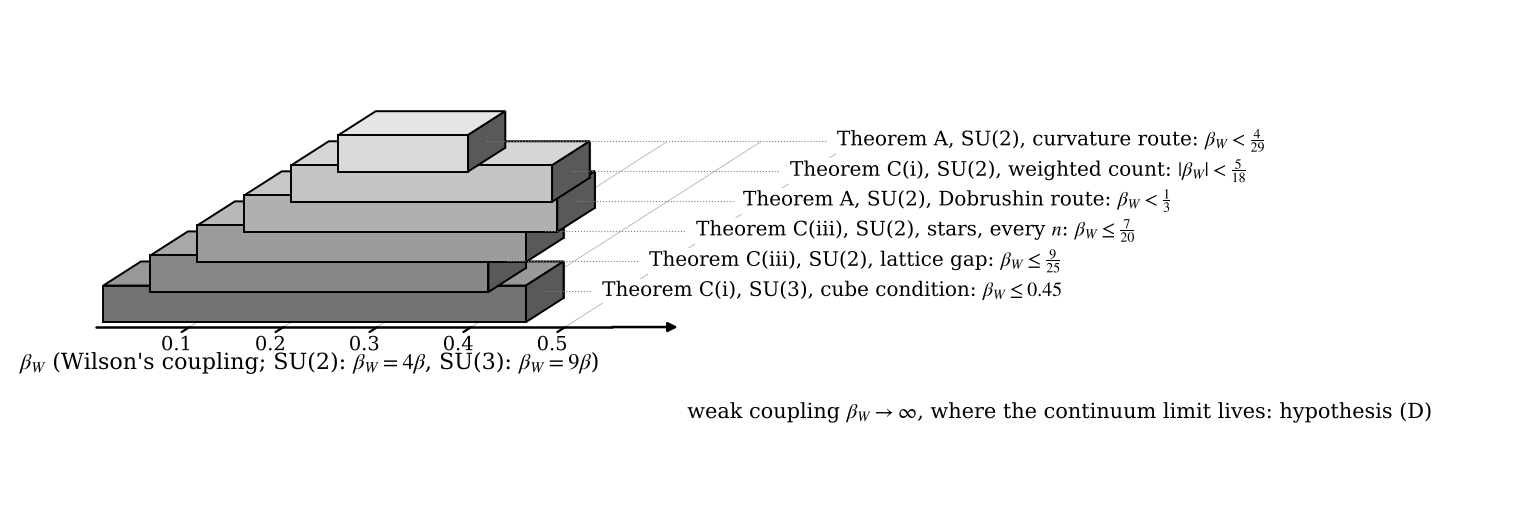
\includegraphics[width=\textwidth]{figures/fig_couplings.png}
\caption{The ranges of Wilson's coupling $\beta_W$ ($\beta_W=4\beta$ for $\SU(2)$, $9\beta$ for $\SU(3)$) covered by the theorems of this paper, from the curvature route of Theorem~\ref{thm:A} to the cube condition of Theorem~\ref{thm:C}(i) for $\SU(3)$; the continuum limit lives at $\beta_W\to\infty$, where (D) is a hypothesis.}
\label{fig:couplings}
\end{figure}

\emph{(c) The group must be non-abelian.} For $G=\U(1)$ with the Villain
action at large $\beta$ the theory is in a massless phase \cite{FS82}: the
gauge-invariant two-point function of the field strength decays only like a
power of the distance. By Theorem~\ref{thm:decay} a cube condition at any
fixed cube size would make that correlation decay exponentially, so the cube
condition fails at every cube size in the Coulomb phase. Every proof of (D)
must therefore use the non-abelian structure of $G$, exactly as a proof of
the mass gap must.

\emph{The two ends.} Ba{\l}aban's renormalisation group
\cite{Bal84a,Bal85a,Bal89b} controls the effective actions of the lattice
theory from the scale $a$ up to scales at which the running coupling is still
small, uniformly in the lattice spacing, in finite volume. The theorems of
Secs.~\ref{sec:curvature}--\ref{sec:bpstrong} control the theory when the
coupling is large: they need $N\beta$ small, that is, $g$ large. The running
coupling grows towards the infrared, so a proof of (D) would follow the
renormalisation group from the weak-coupling regime, where Ba{\l}aban's
estimates hold, through the regime of coupling of order one, to a scale
$\ell$ at which the effective theory satisfies a strong-coupling criterion of
the kind proved here, and would then transport the resulting cube estimate
back to the fine lattice. Neither the middle step nor the final transport is
available: the effective actions are not of Wilson form, Ba{\l}aban's analysis
stops before the coupling is of order one, and no known criterion accepts the
effective theory at that scale. This gap between the two ends is the Yang--Mills
mass gap problem in the form isolated here.

Statement (E) is the construction problem. Ba{\l}aban's ultraviolet stability
bounds give compactness of suitably smeared observables in finite volume, but
the infinite-volume limit, Euclidean invariance and nontriviality of the limit
are open \cite{JW06}. Given (E), Theorem~\ref{thm:B} reduces the mass gap to
(D) with the explicit constant $\Delta\ge16\varpi/(625e^2\ell)$.


\section{The Wilson bound as an exact connected response}\label{cl:sec:replica}

The single-cube criterion concerns partition functions at the same coupling.
It can be written as a connected response without changing that coupling or
replacing the Wilson law by a product law. We give the construction explicitly
for $G=\SU(2)$. Write $b=\beta_W$, so a plaquette contributes
$(b/2)\ReTr Q_p$ to the exponent. All Haar measures below are probability
measures. Fix a spatial torus $s$, let $V=V(s)$, and let $T\ge3$.

\subsection{Two sheets and two cuts}
Take two copies of the time circle $\Z/T\Z$, with sheet labels $a=0,1$.
Choose two distinct cuts, immediately before time $0$ and immediately before
time $d$, where $1\le d<T$. Denote the cuts by $c$ and $c'$.
At each cut introduce four independent temporal-link bundles
$U^{ab}_x\in\SU(2)$, $a,b\in\{0,1\}$, $x\in s$.
An active bundle joins sheet $a$ below the cut to sheet $b$ above it.
If $Q^a_{x,i,-}$ and $Q^b_{x,i,+}$ are the spatial links immediately
below and above the cut, the associated temporal plaquette is
\[
P^{ab}_{x,i}=Q^a_{x,i,-}U^{ab}_{x+e_i}
                 (Q^b_{x,i,+})^*(U^{ab}_x)^*.
\]
For a permutation $\pi$ of the two sheets define the cut action
\[
S_c^\pi=\frac b2\sum_{a=0}^1\sum_{x\in s}\sum_{i=1}^3
                         \ReTr P^{a,\pi(a)}_{x,i}.
\]
Let $S_c^0$ use the identity permutation and $S_c^1$ the transposition;
put $\Delta_c=S_c^1-S_c^0$. Define $S_{c'}^0,S_{c'}^1,\Delta_{c'}$
in the same way. The bulk action contains every other plaquette, including
all spatial plaquettes. On this one fixed product Haar space set
\begin{equation}\label{cl:eq:replica-F}
F(u,v)=\log\int\exp\{S_{\rm bulk}+S_c^0+S_{c'}^0
                              +u\Delta_c+v\Delta_{c'}\}\,dQ,
\qquad 0\le u,v\le1.
\end{equation}
At each corner, an unused bundle has zero action and integrates to one.
With neither cut swapped there are two time circles of length $T$.
With exactly one swapped cut there is one time circle of length $2T$.
With both cuts swapped there are again two length-$T$ circles: relabel
the sheets on the segment between the cuts. Spatial plaquettes are
preserved by this relabelling. Thus
\begin{equation}\label{cl:eq:replica-corners}
F(0,0)=F(1,1)=2\log Z(s,T),\qquad
F(1,0)=F(0,1)=\log Z(s,2T).
\end{equation}
These are exact identities on the finite Wilson lattice, including all
normalisations and all link fields.

\begin{figure}[htbp]
\centering
\begin{tikzpicture}[x=1cm,y=1cm,>=stealth,every node/.style={font=\small}]
\node at (2.5,1.45) {straight matching};
\draw[thick] (0,1)--(2,1);\draw[thick] (3,1)--(5,1);
\draw[thick] (0,0)--(2,0);\draw[thick] (3,0)--(5,0);
\draw[->,thick] (2,1)--(3,1);\draw[->,thick] (2,0)--(3,0);
\node[left] at (0,1) {$a=0$};\node[left] at (0,0) {$a=1$};
\node at (8.5,1.45) {swapped matching};
\draw[thick] (6,1)--(8,1);\draw[thick] (9,1)--(11,1);
\draw[thick] (6,0)--(8,0);\draw[thick] (9,0)--(11,0);
\draw[->,thick] (8,1)--(9,0);\draw[->,thick] (8,0)--(9,1);
\node at (2.5,-.55) {one cut};\node at (8.5,-.55) {one cut};
\end{tikzpicture}
\caption{The two allowed matchings at a cut. There are two independently
switchable cuts on the doubled time circle. Four Haar bundles keep the
integration space fixed throughout the interpolation.}
\label{cl:fig:seams}
\end{figure}

\begin{proposition}[exact replica response]\label{cl:prop:replica}
Let $\operatorname{Cov}_{u,v}$ denote covariance for the probability law
in \eqref{cl:eq:replica-F}. Then
\begin{equation}\label{cl:eq:replica-covariance}
2\psi_s(T)=\int_0^1\!\int_0^1
          \operatorname{Cov}_{u,v}(\Delta_c,\Delta_{c'})\,du\,dv.
\end{equation}
Write $\Delta_c=\sum_x A_x$ and $\Delta_{c'}=\sum_y B_y$, assigning
the three directions and two sheets at each cut to their bottom site.
The quantity
\[
I_{b,s,T}=\int_0^1\!\int_0^1\sum_{y\in s}
                  \operatorname{Cov}_{u,v}(A_0,B_y)\,du\,dv
\]
satisfies $\psi_s(T)=VI_{b,s,T}/2$. In particular, on $s=(2T)^3$,
the datum \Mcirc{} is equivalent to
\begin{equation}\label{cl:eq:replica-target}
I_{b,(2T)^3,T}\le\frac1{16388T^3}.
\end{equation}
\end{proposition}
\begin{proof}
At finite volume the exponent and its derivatives are bounded on the
compact integration space. Differentiating under the integral gives
$\partial_u\partial_vF=\operatorname{Cov}_{u,v}(\Delta_c,\Delta_{c'})$.
The fundamental theorem of calculus and \eqref{cl:eq:replica-corners}
give
\[
\int_{[0,1]^2}\partial_u\partial_vF
=F(1,1)-F(1,0)-F(0,1)+F(0,0)
=4\log Z(s,T)-2\log Z(s,2T)=2\psi_s(T).
\]
The interpolating measure is invariant under spatial translations, so
$\sum_{x,y}\operatorname{Cov}(A_x,B_y)
=V\sum_y\operatorname{Cov}(A_0,B_y)$. This proves the second identity.
For the cube $V=8T^3$, it reads $\psi=4T^3I$; multiplication by
$4097$ gives \eqref{cl:eq:replica-target}.
\end{proof}

The target is a signed integrated covariance bound.\footnote{An absolute
covariance bound would suffice, but it is stronger: the exact identity
permits cancellations both in space and in the interpolation parameters.}
It is not supplied by boundedness of the action. Indeed $|A_x|,|B_y|\le12b$,
because a cut has six plaquettes per bottom site and the difference of
two real traces is at most $4$. Cauchy--Schwarz therefore gives only
$|\operatorname{Cov}(A_x,B_y)|\le144b^2$ and
$|I_{b,s,T}|\le144b^2V$. This grows with the volume, whereas
\eqref{cl:eq:replica-target} decreases as $T^{-3}$.

\subsection{An exact conditional trace factorisation}
There is a second formulation that uses the vacuum measure of the
finite-volume transfer operator. Let $h>0$ be its unit Perron eigenvector,
let $R=\mathbb T/\lambda_0$, and put $\pi(dx)=h(x)^2dx$.
The Markov operator $P=h^{-1}Rh$ is reversible on $L^2(\pi)$.
For an integer $t\ge1$ let $p_t(x,y)$ be the transition density of $P^t$
relative to $\pi$. The kernel is continuous and positive at fixed volume,
so all conditional densities below are defined and finite. Unitary
equivalence and the Hilbert--Schmidt identity give
\begin{equation}\label{cl:eq:chi-trace}
\operatorname{Tr}R^{2t}=\int p_t(x,y)^2\,\pi(dx)\pi(dy).
\end{equation}
Partition the terminal links into $k$ blocks and write $y=(y_1,\ldots,y_k)$.
Let $\ell_j$ be the density of the conditional distribution of $y_j$ under
$P^t(x,dy)$, given $y_1,\ldots,y_{j-1}$, relative to the corresponding
conditional distribution under $\pi$. For each history, this density has
mean one. Set
\[
\chi_j^2(x,y_{<j})=\int(\ell_j-1)^2\,\pi(dy_j\mid y_{<j}),\qquad
S_j=\mathbb E_{\pi\otimes\pi}\prod_{i=1}^j\ell_i^2,
\quad S_0=1.
\]
The conditional-density chain rule gives $\prod_{j=1}^k\ell_j=p_t(x,y)$.
Let $\theta_{j-1}$ be the probability measure on $(x,y_{<j})$ with density
$S_{j-1}^{-1}\prod_{i<j}\ell_i^2$ relative to their
$\pi\otimes\pi$ marginal. Integrating the next block gives
\begin{equation}\label{cl:eq:chi-chain}
\frac{S_j}{S_{j-1}}=1+\mathbb E_{\theta_{j-1}}\chi_j^2,
\qquad
\log\operatorname{Tr}R^{2t}
=\sum_{j=1}^k\log\bigl(1+\mathbb E_{\theta_{j-1}}\chi_j^2\bigr).
\end{equation}
In fact $\int\ell_j^2\,d\pi(\cdot\mid y_{<j})=1+\chi_j^2$;
substitution into $S_j$ proves the first equality, and telescoping with
\eqref{cl:eq:chi-trace} proves the second.

For an even $T=2t$, estimates
\begin{equation}\label{cl:eq:chi-target}
\mathbb E_{\theta_{j-1}}\chi_j^2\le\frac1{8194k}
\quad(1\le j\le k)
\end{equation}
would imply $X_s(T)\le1/8194$, since $\log(1+x)\le x$ for $x\ge0$.
Consequently $\psi_s(T)\le2X_s(T)\le1/4097$.
The measure $\theta_{j-1}$ is essential: an estimate under the untilted
stationary law does not give \eqref{cl:eq:chi-target}.
For an explicit comparison, take the uniform law on four states
$x=(x_1,x_2)\in\{0,1\}^2$ and the reversible transition matrix
$P=\theta I+(1-\theta)J$, where $J(x,y)=1/4$ and $0<\theta<1$.
Reveal the terminal bits in order. Then
$\ell_1=1+\theta$ if $y_1=x_1$, and $\ell_1=1-\theta$ otherwise,
so $S_1=1+\theta^2$. On a matching first-bit history, the two possible
second-bit likelihoods are $1\pm2\theta/(1+\theta)$; on a mismatching
history both are one. Consequently
\[
\mathbb E_{\pi\otimes\pi}\chi_2^2
=\frac{2\theta^2}{(1+\theta)^2},\qquad
\mathbb E_{\theta_1}\chi_2^2
=\frac{(1+\theta)^2}{2S_1}
                       \frac{4\theta^2}{(1+\theta)^2}
=\frac{2\theta^2}{1+\theta^2}.
\]
For $\theta=1/3$ these means are $1/8$ and $1/5$, respectively.
The matrix has eigenvalues $1,\theta,\theta,\theta$, hence
$S_2=\operatorname{Tr}P^2=1+3\theta^2$ and
$S_2/S_1=1+\mathbb E_{\theta_1}\chi_2^2$ as required.
Equations \eqref{cl:eq:replica-target} and \eqref{cl:eq:chi-target}
are concrete analytical targets for the actual Wilson measures.
Neither is established here along the four-dimensional continuum tuning.

\section{Large fields obstruct a global kernel certificate}\label{cl:sec:kernel}

Gauge integration alone does not give a uniform pointwise contraction
estimate at weak coupling. The following calculation uses the complete
$\SU(2)$ Wilson transfer kernel and an explicit admissible large field.
It concerns a global kernel certificate, not the existence of a mass gap.

Let the spatial torus have even side $L\ge6$, and put $V=L^3$.
For spatial link configurations $Q,Q'$ write
\begin{align}
A_b(Q,Q')&=\int\exp\left\{\frac b2\sum_{x,i}
\ReTr\bigl(Q_{x,i}U_{x+e_i}Q_{x,i}'{}^*U_x^*\bigr)\right\}
\prod_xdU_x,\label{cl:eq:kernel-A}\\
\mathbb T_b(Q,Q')&=D_b(Q)A_b(Q,Q')D_b(Q'),\qquad
D_b(Q)=\exp\left\{\frac b4\sum_{p\text{ spatial}}\ReTr Q_p\right\}.
\end{align}
The measure in \eqref{cl:eq:kernel-A} is product probability Haar measure.
\subsection{An explicit gap at every finite coupling and volume}
\begin{proposition}[finite-volume Wilson gap]\label{cl:prop:finite-gap}
For every finite $b>0$ and every spatial torus with sides at least three,
the $\SU(2)$ Wilson transfer operator has a simple largest eigenvalue and
\begin{equation}\label{cl:eq:finite-gap}
r_1\le\tanh\frac{3bV}{2},\qquad
m_{\rm lat}\ge-\log\tanh\frac{3bV}{2}>0.
\end{equation}
At $b=0$ it has rank one. The estimate is valid at weak coupling on each
finite lattice, but is not uniform in physical volume or cutoff.
\end{proposition}
\begin{proof}
For fixed $Q,Q'$, each term of the temporal trace sum in
\eqref{cl:eq:kernel-A} has zero product-Haar mean: the distinct endpoint
variables are independent and the mean of the defining $\SU(2)$
representation is zero. Jensen's inequality therefore gives
$A_b(Q,Q')\ge1$. Each real trace is at most two and there are $3V$
terms, so $A_b(Q,Q')\le B=e^{3bV}$.

Let $h>0$ be the continuous unit Perron eigenfunction of $\mathbb T_b$.
The associated Markov transition has density proportional to
$A_b(Q,Q')D_b(Q')h(Q')$ in its second argument. Thus all its rows are
obtained by weighting one common finite measure by functions in $[1,B]$.
Normalize that common measure to a probability $\nu$. For two such
functions $f,g$ and an event $E$ with $p=\nu(E)$, their normalized laws
$\mu_f,\mu_g$ obey
\[
\mu_f(E)-\mu_g(E)
\le\frac{Bp}{Bp+1-p}-\frac{p}{p+B(1-p)}
=\frac{(B^2-1)p(1-p)}{B+(B-1)^2p(1-p)}
\le\frac{B-1}{B+1}.
\]
The last fraction increases with $p(1-p)\le1/4$. Interchanging $f,g$
gives the same bound for the opposite difference. Hence every pair of
rows has total-variation distance at most
$\tau=(B-1)/(B+1)$, and the Markov operator satisfies
$\operatorname{osc}(Pf)\le\tau\operatorname{osc}(f)$ for bounded real $f$.

For a nonzero excited eigenvalue $r$ of $R=\mathbb T_b/\lambda_0$,
choose a real eigenfunction $u$. It is continuous, since the integral operator maps
$L^2$ into continuous functions. Compactness gives $\min h>0$, so
$u/h$ is bounded and is an eigenfunction of $P$ with eigenvalue $r$.
It is nonconstant. Consequently $r\le\tau$, proving
\eqref{cl:eq:finite-gap} since $\tau=\tanh(3bV/2)$.
Zero eigenvalues do not affect this bound. At $b=0$ the kernel is one,
which proves the rank-one assertion.
\end{proof}

The same estimate holds for every closed subgroup $G\subset\U(N_c)$,
with $b=N_c^2\beta\ge0$ and temporal exponent
$(b/N_c)\sum_e\ReTr(Q_eU_yQ_e'^*U_x^*)$.
Indeed $P_G=\int_Gg\,dg$ is the orthogonal projection onto the invariant
vectors, and $QP_G=P_GQ=P_G$ for $Q\in G$. The product-Haar mean of
each temporal real trace is therefore
$\ReTr(Q_eP_GQ_e'^*P_G)=\operatorname{Tr}P_G\ge0$.
Jensen again gives $A_b\ge1$, and $\ReTr g\le N_c$ gives
$A_b\le e^{3bV}$. Positivity of the transfer operator is
Proposition~\ref{sc:prop:wilson}; the remaining proof is unchanged.
In particular \eqref{cl:eq:finite-gap} holds at every finite positive
coupling and finite volume for every compact simple gauge group.

For a cube of fixed physical side $L$ and cutoff $a$, the volume in
\eqref{cl:eq:finite-gap} is $V=(L/a)^3$. Thus the resulting lower-bound
expression in physical units is
\[
-a^{-1}\log\tanh\!\left(\frac{3b(a)L^3}{2a^3}\right).
\]
It tends to zero as $a\downarrow0$ whenever $b(a)$ is bounded below by a
positive constant, in particular along a weak-coupling tuning. Indeed
$-\log\tanh x=\log((1+e^{-2x})/(1-e^{-2x}))\sim2e^{-2x}$ as
$x\to\infty$. The finite-volume theorem therefore gives no positive
lower bound for the continuum mass. It also does not imply that the
actual mass tends to zero.

\subsection{An admissible large-field witness}
For a positive kernel define its cross-ratio diameter by
\[
\Gamma(K)=\sup_{x,y,u,v}\log
                   \frac{K(x,u)K(y,v)}{K(x,v)K(y,u)}.
\]

\begin{theorem}[a frustrated Wilson-kernel witness]\label{cl:thm:frustrated}
For $b\ge1/4$, the gauge-integrated Wilson kernel satisfies
\begin{equation}\label{cl:eq:diameter-lower}
\Gamma(\mathbb T_b)\ge2V\max\{0,B(b)\},\qquad
B(b)=\frac{3b}{8}-\frac32\log b-\frac32-\log\frac{432\pi}{25}.
\end{equation}
The witness is invariant under passage to gauge orbits and requires no
small-field or chart restriction.
\end{theorem}
\begin{proof}
Let $Q^0_e=I$ for every link, and for $x=(x_1,x_2,x_3)$ put
\[
z_{x,1}=1,\qquad z_{x,2}=(-1)^{x_1},\qquad
z_{x,3}=(-1)^{x_1+x_2},\qquad Q^z_{x,i}=z_{x,i}I.
\]
Evenness of $L$ makes these signs periodic. In each coordinate plane
the product of the four signs on a plaquette is $-1$; hence every
spatial plaquette of $Q^z$ equals $-I$. This configuration is not gauge
equivalent to $Q^0$. Centrality and $z_e^2=1$ give
\[
A_b(Q^0,Q^0)=A_b(Q^z,Q^z)=:A_0,\qquad
A_b(Q^0,Q^z)=A_b(Q^z,Q^0)=:A_z.
\]

Identify $\SU(2)$ with the unit quaternions, using the Euclidean chord
metric $d(g,h)^2=2-\ReTr(gh^*)$. It is bi-invariant, and $d(I,-I)=2$.
For arbitrary temporal variables let $W_{x,i}=U_xz_{x,i}U_{x+e_i}^*$.
Every plaquette of $W$ is $-I$. Its four oriented links $w_1,\ldots,w_4$
therefore satisfy
\[
2\le\sum_{j=1}^4d(I,w_j),\qquad
1\le\sum_{j=1}^4d(I,w_j)^2.
\]
The first inequality is the triangle inequality applied to their
product; the second follows by Cauchy--Schwarz. Each spatial link
belongs to four plaquettes, and there are $3V$ plaquettes. Summing yields
$\sum_ed(I,W_e)^2\ge3V/4$. The mixed temporal real-trace sum is consequently
at most $6V-3V/4=21V/4$. This holds for every temporal field, and gives
\begin{equation}\label{cl:eq:frustrated-upper}
A_z\le\exp(21bV/8).
\end{equation}

For the opposite bound, restrict every $U_x$ to the chord ball
$B_\delta=\{g:d(I,g)\le\delta\}$, $0<\delta\le1$.
Adjacent variables then have distance at most $2\delta$, so the
unfrustrated temporal trace sum is at least $6V-12\delta^2V$.
Writing $g=\cos\theta+\mathbf n\sin\theta$, Haar angle measure is
$(2/\pi)\sin^2\theta\,d\theta$. The interval $0\le\theta\le\delta$
lies in $B_\delta$, and $\sin\theta\ge\theta-\theta^3/6\ge5\theta/6$
there. Hence
\[
\operatorname{Haar}(B_\delta)\ge\frac{25\delta^3}{54\pi},\qquad
A_0\ge\left(\frac{25\delta^3}{54\pi}\right)^V
                  e^{(3b-6b\delta^2)V}.
\]
For $b\ge1/4$ choose $\delta=1/(2\sqrt b)\le1$. Division by
\eqref{cl:eq:frustrated-upper} gives $A_0/A_z\ge e^{VB(b)}$.
All factors $D_b$ cancel from a cross ratio. The choice
$(x,y,u,v)=(Q^0,Q^z,Q^0,Q^z)$ therefore gives
$\Gamma(\mathbb T_b)\ge2\log(A_0/A_z)\ge2VB(b)$.
Also $\Gamma\ge0$, proving \eqref{cl:eq:diameter-lower}.
The kernels are gauge invariant in both arguments, so the same
cross ratio is defined on the gauge quotient.
\end{proof}

\begin{figure}[htbp]
\centering
\begin{tikzpicture}[x=1cm,y=1cm,every node/.style={font=\small}]
\draw[thick] (0,0) rectangle (2,2);\node at (1,1) {$Q_p=I$};
\node at (1,-.45) {flat field $Q^0$};
\draw[thick] (5,0) rectangle (7,2);\node at (6,1) {$Q_p=-I$};
\node[above] at (6,2) {$-I$};\node[below] at (6,0) {$I$};
\node[left] at (5,1) {$I$};\node[right] at (7,1) {$I$};
\node at (6,-.45) {one frustrated plaquette};
\node[align=center] at (3.5,1) {different\\gauge orbits};
\end{tikzpicture}
\caption{A coordinate-plane plaquette of the explicit central-link
field. Every spatial plaquette is frustrated, and temporal gauge
variables cannot remove its chord-energy cost.}
\label{cl:fig:frustration}
\end{figure}

Because $B(b)\to\infty$, a certificate of the form
$\tanh(\Gamma_{\rm upper}/4)$ cannot stay below one uniformly in
coupling and volume: any valid $\Gamma_{\rm upper}$ must obey
\eqref{cl:eq:diameter-lower}.\footnote{Continuity gives the same obstruction
for an essential supremum: every neighbourhood of either witness has
positive product Haar measure. The issue is not an isolated exceptional point.}
This is not a lower bound for the actual subleading eigenvalue.
The equilibrium weight suppresses $Q^z$, and a useful averaged or
multiscale estimate could exploit that suppression. Such an estimate
must control conditional responses as well as probabilities.
For the physical cube $L=2T$, the loss in
\eqref{cl:eq:diameter-lower} is extensive in its actual volume $8T^3$.
It cannot be removed by a scalar normalisation of the transfer matrix.

\section{An exact criterion for retaining a continuum excitation}\label{cl:sec:retention}

A lower spectral gap controls slow decay. It does not prevent every
nonvacuum vector from escaping to infinite physical energy. We separate
these two issues and give the precise Wilson quadratic form that a
trial-observable construction would have to bound.

\begin{proposition}[physical-energy control]\label{cl:prop:retention}
For $a\downarrow0$, let $R_a$ be a nonnegative self-adjoint contraction
with a unit vacuum $\Omega_a$, $R_a\Omega_a=\Omega_a$. Let
$\psi_a\perp\Omega_a$ and $v_a=\|\psi_a\|^2$. Suppose
\begin{equation}\label{cl:eq:trial-energy}
0<v_*\le v_a\le V_*<\infty,\qquad
\langle\psi_a,(I-R_a)\psi_a\rangle\le aE_*v_a
\end{equation}
for a finite $E_*>0$. If $aE_*<1$, then for every integer $n\ge1$,
\[
\langle\psi_a,R_a^n\psi_a\rangle\ge v_a(1-aE_*)^n.
\]
For each fixed physical $t>0$ this implies
\begin{equation}\label{cl:eq:retention-limit}
\liminf_{a\downarrow0}
\langle\psi_a,R_a^{\lceil t/a\rceil}\psi_a\rangle
\ge v_*e^{-E_*t}>0.
\end{equation}
\end{proposition}
\begin{proof}
Let $\nu_a$ be the probability spectral measure of $R_a$ in
$\psi_a/\sqrt{v_a}$, supported on $[0,1]$. The last inequality in
\eqref{cl:eq:trial-energy} gives $\int r\,d\nu_a\ge1-aE_*$.
Convexity of $r\mapsto r^n$ gives
$\int r^n\,d\nu_a\ge(\int r\,d\nu_a)^n\ge(1-aE_*)^n$.
For $n=\lceil t/a\rceil$ one has $na\to t$ and
$n\log(1-aE_*)\to-E_*t$, which proves
\eqref{cl:eq:retention-limit}. No logarithm of $R_a$ is needed, so
the spectral measure may have mass at zero. If $E_*=0$, the measure
is concentrated at $r=1$ and the correlation is identically $v_a$.
\end{proof}

\begin{proposition}[filtering a retained vector]\label{cl:prop:filtering}
Let $H_a\ge0$, $\psi_a\perp\Omega_a$, $\|\psi_a\|^2\le V_*$.
Suppose for a fixed $s>0$ that
$\langle\psi_a,e^{-2sH_a}\psi_a\rangle\ge c_*>0$.
For $\chi_a=e^{-sH_a}\psi_a$,
\[
\|\chi_a\|^2\ge c_*,\qquad
\langle\chi_a,H_a\chi_a\rangle\le\frac{V_*}{2es},\qquad
\frac{\langle\chi_a,H_a\chi_a\rangle}{\|\chi_a\|^2}
\le\frac{V_*}{2es c_*}.
\]
\end{proposition}
\begin{proof}
The norm is the assumed correlation. The energy numerator is the
integral of $E e^{-2sE}$ against the spectral measure in $\psi_a$.
This function has maximum $1/(2es)$ at $E=1/(2s)$, and the total
spectral mass is at most $V_*$. Division by the norm lower bound
proves the last inequality.
\end{proof}

Filtering is a vector construction over a fixed physical time interval.
It does not establish the assumed correlation, and it does not turn
the vector into a fixed-stencil local token.\footnote{A fixed physical
smear or loop generally involves a number of lattice links that grows
as the cutoff is removed. Its admissibility and renormalisation must
be checked in the chosen continuum reconstruction.}

\subsection{The exact Wilson Dirichlet form}
At each finite cutoff and volume let $T_a(Q,Q')$ be the positive
Wilson transfer kernel, with unit positive eigenfunction $\Omega_a$
and top eigenvalue $\lambda_a$. Define
\[
\pi_a(dQ)=\Omega_a(Q)^2dQ,\qquad
P_a(Q,dQ')=\frac{T_a(Q,Q')\Omega_a(Q')}
                         {\lambda_a\Omega_a(Q)}\,dQ'.
\]
The eigenvalue equation makes $P_a$ a probability kernel, and symmetry
of $T_a$ gives detailed balance. Multiplication by $\Omega_a$ is a
unitary map from $L^2(\pi_a)$ to the transfer Hilbert space, intertwining
$P_a$ with $R_a=T_a/\lambda_a$. Thus for every $f\in L^2(\pi_a)$,
\begin{equation}\label{cl:eq:wilson-dirichlet}
\langle\Omega_af,(I-R_a)\Omega_af\rangle
=\frac12\iint|f(Q)-f(Q')|^2\,\pi_a(dQ)P_a(Q,dQ').
\end{equation}
To verify the identity, expand the square. Stationarity gives
$\int|f|^2d\pi_a$ for each square term, while the two cross terms
give twice $\operatorname{Re}\langle f,P_af\rangle$.
Reversibility makes this inner product real, and unitary equivalence
gives \eqref{cl:eq:wilson-dirichlet}.

For a centered gauge-invariant observable $f_a$, a sufficient concrete
construction for retention would therefore be
\begin{align}
v_*\le\operatorname{Var}_{\pi_a}(f_a)&\le V_*,\label{cl:eq:variance-target}\\
\frac12\iint|f_a(Q)-f_a(Q')|^2\,\pi_a(dQ)P_a(Q,dQ')
&\le aE_*\operatorname{Var}_{\pi_a}(f_a).\label{cl:eq:dirichlet-target}
\end{align}
These estimates must be uniform along the actual tuning and the
required volume limits. Proposition~\ref{cl:prop:retention} would
then give a positive fixed-distance two-point function, provided that
observable is among the limits defining the continuum theory.
Neither \eqref{cl:eq:variance-target} nor
\eqref{cl:eq:dirichlet-target} is proved here for that Wilson family.
Choosing an excited eigenfunction rewrites the required energy
estimate; it does not prove it.

\subsection{Retention without an upper bound on the whole trial energy}
The Dirichlet estimate above is sufficient. An observable can retain a
finite-energy component even when another component escapes to arbitrarily
high energy. The following equivalence isolates exactly what must remain.

\begin{proposition}[bounded-energy spectral mass]\label{cl:prop:spectral-mass}
Let $H_a\ge0$, $\psi_a\perp\Omega_a$ and $\|\psi_a\|^2\le V_*<\infty$.
Write $\nu_a(B)=\langle\psi_a,\mathbf1_B(H_a)\psi_a\rangle$.
The following statements are equivalent, with constants uniform for all
sufficiently small $a$:
\begin{enumerate}[label=\textup{(\roman*)},leftmargin=*]
\item At one fixed physical time $t>0$,
$\langle\psi_a,e^{-tH_a}\psi_a\rangle\ge c_*>0$.
\item There exist $E_*<\infty$ and $\eta_*>0$ such that
$\nu_a([0,E_*])\ge\eta_*$.
\end{enumerate}
More precisely, \textup{(i)} implies
\[
\nu_a([0,E])\ge c_*-V_*e^{-tE}
\qquad(E>0),
\]
and \textup{(ii)} implies a correlation lower bound
$\eta_*e^{-uE_*}$ at every fixed physical time $u\ge0$.
\end{proposition}
\begin{proof}
Split the spectral integral at $E$. Its part below $E$ is at most
$\nu_a([0,E])$, and its part above $E$ is at most $V_*e^{-tE}$.
For $E=t^{-1}\log(2V_*/c_*)$, the first implication gives a spectral
mass of at least $c_*/2$. Conversely $e^{-u\lambda}\ge e^{-uE_*}$ on
$[0,E_*]$, which proves the second implication. The assumption
$\psi_a\perp\Omega_a$ removes the vacuum contribution; it does not
remove any additional low-energy excited spectral mass.
\end{proof}

The spectral projection $\mathbf1_{[0,E_*]}(H_a)\psi_a$ then has squared
norm at least $\eta_*$ and energy quotient at most $E_*$.
This is a Hilbert-space construction after the spectral-mass bound has
been proved, and is not a construction of a local field. It allows the
retention problem to be attacked without bounding the energy of an
entire unfiltered observable. To see the distinction, take an excited
spectral measure
\[
\nu_a=\tfrac12\delta_1+\tfrac12\delta_{a^{-2}},\qquad R_a=e^{-aH_a}.
\]
Its correlation is at least $e^{-t}/2$ at every $t>0$, while
\[
a^{-1}\langle\psi_a,(I-R_a)\psi_a\rangle
=\frac{1-e^{-a}}{2a}+\frac{1-e^{-1/a}}{2a}\longrightarrow\infty.
\]
Thus the raw Dirichlet quotient in \eqref{cl:eq:trial-energy} need not
remain bounded for a retained vector. Proposition~\ref{cl:prop:spectral-mass}
does not prove its hypothesis for a Wilson observable; it identifies a
weaker, necessary and sufficient spectral target.

\begin{figure}[htbp]
\centering
\begin{tikzpicture}[>=stealth,every node/.style={align=center,font=\small}]
\node[draw,rounded corners,text width=3.1cm] (a) at (0,0)
{variance lower bound\\and energy upper bound};
\node[draw,rounded corners,text width=3.1cm] (b) at (4.25,0)
{positive correlation\\at fixed physical time};
\node[draw,rounded corners,text width=3.1cm] (c) at (8.5,0)
{a nonvacuum vector\\in a compatible limit};
\draw[->,thick] (a)--node[above] {Jensen} (b);
\draw[->,thick] (b)--node[above] {convergence} (c);
\end{tikzpicture}
\caption{Energy retention is a separate obligation from a lower
spectral gap. The first arrow is Proposition~\ref{cl:prop:retention};
the second also requires a continuum reconstruction containing these
correlations.}
\label{cl:fig:retention}
\end{figure}

\subsection{A gap does not by itself give nontriviality}
On $\C^2$, let $\Omega=(1,0)$, $\psi=(0,1)$ and
$R_a=\operatorname{diag}(1,e^{-\sqrt a})$.
The only excitation has physical energy $a^{-1/2}\ge1$ for $a\le1$,
and $\|\psi\|=1$. Nevertheless
\[
\langle\psi,R_a^{\lceil t/a\rceil}\psi\rangle
=e^{-\sqrt a\,\lceil t/a\rceil}\longrightarrow0
\qquad(t>0).
\]
The thermal trace tends to one at every fixed positive physical
inverse temperature. This is a spectral counterexample, not a Wilson
model. It shows precisely why a lower gap and unit normalisation do
not supply \eqref{cl:eq:dirichlet-target}: here
$a^{-1}\langle\psi,(I-R_a)\psi\rangle\sim a^{-1/2}$ diverges.

Nonzero retained two-point functions would still not prove the full
Yang--Mills identification or the remaining reconstruction axioms.
For example, if all moments of four centered separated smears converge,
their connected four-point function is the limit of the fourth moment
minus the three products of paired second moments. A uniform positive
lower bound on its absolute value would exclude a jointly Gaussian
law for those particular fields. Upper moment bounds alone give no
such lower bound. Moreover composite fields in a free theory can have
nonzero fourth cumulants, so this test alone does not establish an
interacting Yang--Mills theory.

\section{Conditional Wilson inequalities and a score criterion}\label{cl:sec:fisher}

The trace identity of Section~\ref{cl:sec:replica} requires a bound under
squared-likelihood tilted histories. We first prove a conditional
inequality for the actual Wilson vacuum, without a restriction to calm
fields, and then use it to obtain a sufficient score estimate for the
cube datum. The conditional inequality is uniform in volume. The score
estimate still requires control across a physical time interval.

\subsection{Every one-link conditional vacuum law}
Let $s$ be a three-dimensional spatial torus whose sides are at least three,
and let $b=\beta_W\ge0$. Use the exact $\SU(2)$ transfer kernel
\eqref{cl:eq:kernel-A}, with
\[
S_{\rm sp}(Q)=\frac b2\sum_{p\text{ spatial}}\ReTr Q_p,
\qquad D_b(Q)=e^{S_{\rm sp}(Q)/2}.
\]
Let $h_b>0$ be its unit Perron eigenfunction and
$\pi_b(dQ)=h_b(Q)^2dQ$. Order the spatial links arbitrarily. A prefix
history fixes an initial segment of this order; all later links remain
integrated over. Each $\SU(2)$ factor in this section has the unit-round
$S^3$ metric.\footnote{This metric convention applies to the gradients in
this section. The metric $-\Tr(XY)$ used for curvature earlier in the
paper is twice the unit-round metric on $\SU(2)$. A constant rescaling
of the metric rescales both the Poincar\'e constant and the squared
gradient inversely, leaving their product unchanged.}

\begin{theorem}[conditional vacuum comparison]\label{cl:thm:link-poincare}
For every finite $b\ge0$, every link ordering and every prefix history,
the conditional density $\rho_j$ of the next link relative to probability
Haar measure obeys
\begin{equation}\label{cl:eq:prefix-density}
\frac{\rho_j(u)}{\rho_j(v)}\le e^{12b}
\qquad(u,v\in\SU(2)).
\end{equation}
Consequently every smooth real $f$ on that link satisfies
\begin{equation}\label{cl:eq:prefix-poincare}
\operatorname{Var}_{\pi_{b,j}}(f)
\le \frac{e^{12b}}3\int |\nabla f|^2\,d\pi_{b,j}.
\end{equation}
The constants are independent of spatial volume and the prefix history.
\end{theorem}
\begin{proof}
Suppose $Q,\widetilde Q$ differ on one spatial link. That link belongs
to four spatial plaquettes. Each contribution $(b/2)\ReTr Q_p$ lies in
$[-b,b]$, hence
\[
|S_{\rm sp}(Q)-S_{\rm sp}(\widetilde Q)|\le8b.
\]
For fixed $Q'$ and temporal links, exactly one term in the temporal
action contains the changed bottom link. Its change is at most $2b$.
Comparison before the temporal Haar integration therefore gives
\[
e^{-2b}\le\frac{A_b(Q,Q')}{A_b(\widetilde Q,Q')}\le e^{2b}.
\]
Put $g_b=h_b/D_b$. The Perron equation reads
\[
\lambda_b g_b(Q)=\int A_b(Q,Q')D_b(Q')h_b(Q')\,dQ'.
\]
Its integrand, apart from $A_b$, has a positive weight independent of $Q$.
Thus $g_b(Q)/g_b(\widetilde Q)$ lies in $[e^{-2b},e^{2b}]$.
As $h_b^2=e^{S_{\rm sp}}g_b^2$, we obtain
\begin{equation}\label{cl:eq:vacuum-local-ratio}
e^{-12b}\le\frac{h_b(Q)^2}{h_b(\widetilde Q)^2}\le e^{12b}.
\end{equation}
Fix any prefix, replace the next link $u$ by $v$, and integrate all
unrevealed links with product Haar measure. The same bounds hold pointwise
before integration, and hence after integration. Normalising the
conditional law cancels in the density ratio. This proves
\eqref{cl:eq:prefix-density} for every history. All densities are smooth
and positive: the kernel is smooth and positive on a compact space, and
the Perron equation preserves smoothness.

On the unit round $S^3$, Haar measure has Poincar\'e constant $1/3$.
Indeed the eigenvalues of $-\Delta_{S^3}$ on restrictions of homogeneous
harmonic polynomials of degree $r$ are $r(r+2)$. This follows by writing
the Euclidean Laplacian in polar coordinates and applying it to
$R^rY(\omega)$. Harmonic decomposition of polynomials and density of their
restrictions in $L^2(S^3)$ give a complete orthogonal decomposition;
the least nonconstant eigenvalue is therefore $3$.
If $m=\min\rho_j$ and $M=\max\rho_j$, then $M/m\le e^{12b}$.
Writing $\sigma$ for probability Haar measure and taking its mean as a
comparison constant in the variance gives
\[
\operatorname{Var}_{\rho_j\sigma}f
\le M\operatorname{Var}_{\sigma}f
\le \frac M3\int|\nabla f|^2d\sigma
\le \frac{M}{3m}\int|\nabla f|^2\rho_jd\sigma.
\]
This is \eqref{cl:eq:prefix-poincare}.
\end{proof}

No coupling-dependent excluded set occurs in this proof. In particular,
large fields remain in every integral. The result concerns prefix
conditionals of the unconditioned vacuum law. It does not assert a
Poincar\'e inequality on a chart, a label-restricted set or a prescribed
coarse-field fibre, whose support can be disconnected. Nor can the
one-link inequalities be tensorised without a separate control of
dependence between links.

The proof also applies to a compact connected matrix group
$G\subset\U(N_c)$ with temporal coefficient $b/N_c$. Each normalised
plaquette term still lies in $[-b,b]$, and each spatial link still belongs
to four spatial plaquettes. If $C_G$ is a Haar Poincar\'e constant for a
chosen bi-invariant metric, the conditional constant is at most
$C_Ge^{12b}$. Connectedness matters here; a gradient-only Poincar\'e
inequality cannot control different components of a disconnected group.

\subsection{From conditional variance to a tilted score budget}
Let $y=(y_1,\ldots,y_k)$ be an ordering of the terminal links, and retain
$\ell_j,S_j,\theta_{j-1}$ from \eqref{cl:eq:chi-chain}. Let $\theta_j$
be the law on $(x,y_{\le j})$ whose density relative to the corresponding
$\pi\otimes\pi$ marginal is
\[
S_j^{-1}\prod_{i=1}^j\ell_i^2.
\]
In contrast to $\theta_{j-1}$, this law includes the next revealed link
$y_j$. The gradient $\nabla_j$ below acts on that link with its history
held fixed.

\begin{proposition}[conditional score bound]\label{cl:prop:fisher-chain}
Suppose the conditional law $\pi_j(dy_j\mid y_{<j})$ has Poincar\'e
constant at most a finite measurable $C_j(x,y_{<j})$. Define
\[
\eta_j=\mathbb E_{\theta_j}
       \bigl[C_j(x,y_{<j})|\nabla_j\log\ell_j|^2\bigr].
\]
If $0\le\eta_j<1$ for every $j$, then
\begin{equation}\label{cl:eq:fisher-log}
\log\operatorname{Tr}R^{2t}
\le\sum_{j=1}^k-\log(1-\eta_j).
\end{equation}
If also $\delta=\sum_j\eta_j<1$, then
\begin{equation}\label{cl:eq:fisher-total}
\log\operatorname{Tr}R^{2t}
\le-\log(1-\delta)\le\frac{\delta}{1-\delta}.
\end{equation}
\end{proposition}
\begin{proof}
Each conditional density $\ell_j$ has mean one. Its variance is therefore
$\chi_j^2$. Apply the conditional Poincar\'e inequality to $\ell_j$,
multiply by $\prod_{i<j}\ell_i^2$ and integrate. With the base measure
$\pi\otimes\pi$ this gives
\[
S_j-S_{j-1}
\le\int\!\left(\prod_{i<j}\ell_i^2\right)C_j|\nabla_j\ell_j|^2
=S_j\eta_j.
\]
The last equality uses strict positivity and
$\nabla\ell_j=\ell_j\nabla\log\ell_j$. Hence
$S_j/S_{j-1}\le(1-\eta_j)^{-1}$. Multiplication over $j$ and the exact
identity $S_k=\operatorname{Tr}R^{2t}$ prove \eqref{cl:eq:fisher-log}.
Induction gives $\prod_j(1-\eta_j)\ge1-\sum_j\eta_j$ for nonnegative
$\eta_j$ whose sum is below one. Finally
\[
-\log(1-\delta)=\int_0^\delta\frac{du}{1-u}
\le\frac{\delta}{1-\delta},
\]
which proves \eqref{cl:eq:fisher-total}.
\end{proof}

\begin{corollary}[a sufficient Wilson score estimate]\label{cl:cor:wilson-score}
On the $\SU(2)$ spatial cube $s=(2T)^3$, with even $T=2t\ge4$, suppose
the actual Wilson transition and vacuum law satisfy
\begin{equation}\label{cl:eq:wilson-score-target}
\sum_{j=1}^{3V(s)}\mathbb E_{\theta_j}
       |\nabla_j\log\ell_j|^2\le\frac{3e^{-12b}}{8195}.
\end{equation}
Then $X_s(T)\le1/8194$ and $\psi_s(T)\le1/4097$, so \Mcirc{} holds.
\end{corollary}
\begin{proof}
Take $C_j=e^{12b}/3$ from Theorem~\ref{cl:thm:link-poincare}.
Then $\delta\le1/8195$, and
$\delta/(1-\delta)\le1/8194$. Proposition~\ref{cl:prop:fisher-chain}
and $X_s(T)=\log\operatorname{Tr}R^T$ give the first bound. Since
$\psi_s(T)=2X_s(T)-X_s(2T)$ and $X_s(2T)\ge0$, the second follows.
\end{proof}

\begin{figure}[htbp]
\centering
\begin{tikzpicture}[>=stealth,every node/.style={font=\small,align=center}]
\node[draw,rounded corners,text width=3cm] (a) at (0,0)
{one-link density ratio\\$\rho_j(u)/\rho_j(v)\le e^{12b}$};
\node[draw,rounded corners,text width=3cm] (b) at (4.1,0)
{conditional Poincar\'e\\$C_j\le e^{12b}/3$};
\node[draw,rounded corners,text width=3cm] (c) at (8.2,0)
{thermal trace bound\\$X_s(T)\le\delta/(1-\delta)$};
\draw[->,thick] (a)--node[above]{proved} (b);
\draw[->,thick] (b)--node[above]{score budget} (c);
\node[text width=7cm] at (6.1,-1.3)
{The score budget in \eqref{cl:eq:wilson-score-target} remains unproved
along the continuum tuning.};
\end{tikzpicture}
\caption{The conditional comparison is independent of volume and includes
all link fields. Its use in the cube criterion also requires decay of
the transition likelihood scores over a physical time interval.}
\label{cl:fig:fisher}
\end{figure}

The corollary separates two estimates. The conditional comparison has
been proved for every finite coupling. The time-dependent score budget
\eqref{cl:eq:wilson-score-target} has not. The factor $e^{12b}$ grows
along weak-coupling tuning; it cannot be hidden in a cutoff-independent
constant. Even a fixed physical cube has $3V(s)=24T^3$ revealed links,
so a bound on each score that is merely uniform in $j$ is insufficient.
A block ordering with a better conditional constant, a genuinely
time-decaying score bound or direct cancellation in the signed response
\eqref{cl:eq:replica-covariance} would require further estimates.

\subsection{The accuracy required of a free-energy remainder}
The leading weak-coupling free energy is a bulk quantity. Recent explicit
evaluation of its Maxwell constant \cite{Bre26} does not by itself
control the thermal defect. To quantify the distinction, fix the same
spatial torus and coupling and suppose
\[
\log Z(s,T)=VTf(b)+r_T,\qquad
\log Z(s,2T)=2VTf(b)+r_{2T}.
\]
The cancellation is exact: $\psi_s(T)=2r_T-r_{2T}$. Separate estimates
$|r_T|\le\varepsilon VT$ and $|r_{2T}|\le2\varepsilon VT$ give only
\[
\psi_{(2T)^3}(T)\le4\varepsilon VT=32\varepsilon T^4.
\]
Thus this method would require $\varepsilon\le1/(131104T^4)$ to prove
\Mcirc{}. A remainder stated only as $o(1)$ in the free-energy density
has no such rate. These error assumptions concern the periodic boxes
actually used here; asymptotics with other boundary conditions need an
additional boundary comparison. Likewise the weak-coupling decay theorem
for finite gauge groups \cite{AC25} supplies no uniform estimate for
continuous $\SU(2)$ merely by replacing the group in its statement.

\section{A bounded seam observable on one spatial cube}\label{cl:sec:bounded-seam}

Consider the two temporal cuts in Section~\ref{cl:sec:replica}. At each cut
choose a matching sign $\sigma,\tau\in\{-1,1\}$, with equal independent
prior probabilities, as in the Anaxia replica-seam construction.%
\footnote{The construction workspace is linked in Data and Code Availability.}
Conditional on the signs, use the corresponding
Wilson weight on both sheets and integrate all links against Haar measure.
The probability below is taken after jointly normalising the four
weighted ensembles. The argument applies to each Wilson group in
Proposition~\ref{sc:prop:wilson}: relabelling the sheets preserves the
plaquette traces and inactive Haar bundles have integral one.

For a fixed spatial box $s$, write $A=Z(s,T)^2$ and $B=Z(s,2T)$.
Each equal-sign corner has weight proportional to $A$, and each
opposite-sign corner has weight proportional to $B$. Thus the probability
of different matchings and the correlation of the signs are
\begin{equation}\label{cl:eq:seam-disagreement}
 p_{\rm diff}=\frac{B}{A+B},\qquad
 \mathbb E[\sigma\tau]=1-2p_{\rm diff}=\tanh\bigl(\psi_s(T)/2\bigr).
\end{equation}
The signs have mean zero. This identity concerns the Wilson-weighted
probability. The prior probability of disagreement is $1/2$.

\begin{theorem}[A single seam-disagreement test]\label{cl:thm:seam-disagreement}
Fix an integer $T\ge3$ and one bare coupling. If
\begin{equation}\label{cl:eq:two-fifths}
 p_{\rm diff}\ge 2/5 \quad\hbox{on the spatial cube } (24T)^3,
\end{equation}
then, writing $q=3^{-1/7}$, every spatial cube of integer side $n\ge24T$
satisfies
\[
 r_1(n^3)\le q^{1/T},\qquad
 \Dexc{n^3}{n}\le q^{n/T}.
\]
Suppose there is $t_0>0$ such that for all sufficiently large $p$ and,
for each such $p$, all sufficiently large $N$ in its mesh sequence,
\eqref{cl:eq:two-fifths} holds at the actual coupling $\beta_{N,p}$ for
some integer $3\le T\le Nt_0$. The physical gap in a compatible Wightman
limit under hypothesis \textup{(W)} is then at least $\log(3)/(7t_0)$.
\end{theorem}
\begin{proof}
Put $x_j=r_j(s)^T$ for the excited eigenvalues, counted with multiplicity,
$D=\sum_{j\ge1}x_j$ and $E=\sum_{j\ge1}x_j^2$. Equation
\eqref{cl:eq:two-fifths} yields $(1+D)^2/(1+E)=A/B\le3/2$.
Since $E\le D$, this first gives $D\le1/2$. Since also $E\le D^2$,
it gives $D^2-4D+1\ge0$. Hence $D\le2-\sqrt3<2/7=:d$.

Let $T_i=8^iT$, and put $D_i=\Dexc{(24T_i)^3}{T_i}$.
Raise the transfer operator to a higher power on the \emph{same} box
before enlarging that box. Positivity of the excited weights gives
$\Dexc{(24T_i)^3}{8T_i}\le D_i^8$. At time $8T_i$ apply
Theorem~\ref{sc:thm:cube-control} with initial spatial sides $24T_i$.
For each integer $24T_i\le n\le192T_i$ the enlargement factor is at
most $(192/16)^3=1728$. It follows that
\begin{equation}\label{cl:eq:eightfold-bound}
 \Dexc{n^3}{8T_i}\le(1+D_i^8)^{1728}-1.
\end{equation}
The endpoint $n=192T_i$ gives $D_{i+1}$ on the left.
For $0\le x\le d$ one has $1728d^8<1/8$ and therefore
\[
 (1+x^8)^{1728}-1
 \le e^{1728x^8}-1
 \le \frac{1728x^8}{1-1728d^8}\le2048x^8 .
\]
Also $2048d^7=262144/823543<1/3$. Induction gives
$D_i\le d q^{8^i-1}$: if this holds at $i$, the right-hand side of
\eqref{cl:eq:eightfold-bound} is at most
$d(2048d^7)q^{8(8^i-1)}\le d q^{8^{i+1}-1}$.

For any $n\ge24T$ take $i$ with $24T_i\le n<192T_i$. Since $d<q$,
\eqref{cl:eq:eightfold-bound} gives
$r_1(n^3)^{8T_i}\le\Dexc{n^3}{8T_i}\le q^{8^{i+1}}$.
Taking the $8T_i$-th root gives the claimed eigenvalue bound. Multiplying
each term of the excited trace by the remaining power of its eigenvalue
gives $\Dexc{n^3}{n}\le q^{8^{i+1}}q^{(n-8T_i)/T}=q^{n/T}$.
On $n=NL_p$, once $L_p\ge24t_0$, these bounds give
$r_1\le e^{-\Delta/N}$ and $\Dexc{n^3}{n}\le e^{-\Delta L_p}$ with
$\Delta=\log(3)/(7t_0)$. The first gives the exponential bound on
centered transfer matrix elements and the second removes the excited
thermal trace in the large-volume limit. The thermal comparison and
spectral argument in the proof of Theorem~\ref{sc:thm:continuum}
now apply under the same hypothesis \textup{(W)}.
\end{proof}

An elementary bound for the actual Wilson ensemble illustrates the scale
of \eqref{cl:eq:two-fifths}. Write $b=N_c^2\beta$, so each plaquette
term in the exponent lies in $[-b,b]$. Switching one cut changes six
terms per spatial site (three directions on each sheet). The exponent
changes by at most $12bV$ on the common link space. Integrating gives
$A/B\le e^{12bV}$ and hence $p_{\rm diff}\ge(1+e^{12bV})^{-1}$.
This lower bound tends to zero on expanding weak-coupling cubes.
Improving it to $2/5$ requires control of the integrated response
between the cuts.

This test retains information about all excited states. For illustration,
take the even occupation numbers of one free massless lattice oscillator
of momentum $2\pi/(24T)$, with the vacuum energy subtracted. Its energy
spacing before the even projection is
$E_1=2\operatorname{arsinh}(\sin(\pi/(24T)))\le\pi/(12T)$.
Writing $z=e^{-2TE_1}$, the two traces are $(1-z)^{-1}$ and
$(1-z^2)^{-1}$. Formula~\eqref{cl:eq:seam-disagreement} gives
$1-2p_{\rm diff}=z\ge e^{-\pi/6}>1/5$. Even this single oscillator
fails \eqref{cl:eq:two-fifths}. The interacting Wilson probability along
the tuning requires an independent estimate. No estimate of that
probability follows from the prior on the matching signs or from the
one-link vacuum comparison.

\section{Conclusion}\label{sec:conclusion}

For unequal couplings the partition ratio itself can be bounded:
Theorem~\ref{cl:thm:unequal-gap} gives a physical lattice gap uniform
in spatial volume. The continuous-time $\SU(2)$ result also retains
spectral weight at a finite energy in a gauge-invariant observable.
Extending that proof to the isotropic tuning would require controlling
the spatial plaquette action when its coefficient grows along with the
temporal one; the absolute expansion in Section~\ref{cl:sec:unequal}
loses smallness in precisely that regime.

The strengthened criterion of Theorem~\ref{sc:thm:continuum} replaces the
window of tori by one cube: the inequality
$\psi_{(2T_0)^3}(T_0)\le1/4097$ at $T_0\le Nt_0$ implies
$\Delta=t_0^{-1}\log(63/32)$. The proof derives vacuum dominance and the
lattice-to-physical spectral conversion directly from that datum. The
zero--one law of Theorem~\ref{sc:thm:zero-one} further shows that the
normalised physical cube pressure either stays above a fixed threshold
at every scale or enters the exponentially decaying branch. It does not
select the branch of the tuned Wilson system.

Theorem~\ref{cl:thm:rough-cells} controls joint rough-cell events at weak
coupling. On even cubes the removal of all rough clusters of size at
least half the time period changes the seam probability by the explicit
error in Corollary~\ref{cl:cor:seam-clusters}. It remains to compare the
weights of the two matchings on the retained configurations. On the cube
of side $24T$, Theorem~\ref{cl:thm:seam-aspect} reduces the sufficient
unconditional seam probability to $97/266$. Proposition~\ref{cl:prop:seam-winding}
shows why the comparison has to average over the spatial fields.
For $\SU(2)$, Proposition~\ref{cl:prop:row-pins} permits all straight
windings in one spatial direction to be fixed to the identity with a
vanishing error in that comparison when $n/(1+4b)-3\log n\to+\infty$.
The remaining integrals couple the transverse layers at the original
Wilson coupling. Theorem~\ref{cl:thm:charged-gap} bounds the charged
spectrum uniformly in volume for every compact connected matrix group;
the gauge-invariant excited spectrum remains the physical target.
At $T\asymp N$ and $b=O(\log N)$ the same seam odds can be computed
before gauge projection with error smaller than every inverse power of
$N$ (Corollary~\ref{cl:cor:temporal-physical}).

The replica construction gives the exact single-cube target
$I_{b,(2T)^3,T}\le1/(16388T^3)$. Its conditional trace counterpart
requires bounds in squared-likelihood tilted histories, rather than the
stationary average alone. The large-field witness rules out a uniform
global diameter certificate, and the Wilson Dirichlet identity isolates
the upper energy and lower variance estimates needed to retain a
continuum excitation. None of these identities supplies the corresponding
uniform estimate for the tuned Wilson measure.


The conditional Wilson comparison of Theorem~\ref{cl:thm:link-poincare}
is independent of volume and includes every prefix history. Its constant
grows as $e^{12b}$, so it does not supply a coupling-uniform gap.
Corollary~\ref{cl:cor:wilson-score} identifies the remaining score budget
that would suffice for the single-cube datum. The bounded-energy
criterion of Proposition~\ref{cl:prop:spectral-mass} permits retained
observables with a divergent high-energy component, and
Appendix~\ref{cl:app:flow} gives a regularisation that preserves
positive-time support. Neither construction proves the required
Wilson spectral-mass lower bound or the continuum convergence estimates.

The full four-dimensional weak-coupling problem remains unresolved:
the datum must still be proved along the continuum tuning, and a
nontrivial continuum theory satisfying the required axioms must be
constructed for every compact simple group. The single-cube criterion
complements the following strong-coupling and slab results.



Lattice Yang--Mills theory in four dimensions has a mass gap with the explicit
lower bound $m_G(\beta)$ for every compact simple gauge group in the range
$N\beta<\frac2{29}\kappa_G$, and for $\SU(2)$ up to $\beta_W=\frac13$ with
the bound $-\log(3\beta_W)$ and up to $\beta_W=\frac9{25}$ by resampling stars. A
single
spectral gap $\varpi$ of the dynamics that resamples cubes of a fixed physical
size $\ell$, uniform along the continuum tuning, gives every nontrivial
continuum limit the mass gap $16\varpi/(625e^2\ell)$. That spectral gap holds
at strong coupling, for $\SU(2)$ up to $\beta_W=\frac7{20}$ uniformly in the
cube size and for $\SU(3)$ up to $\beta_W=0.45$, and for massive free fields;
it fails for massless fields, at fixed cube size at weak coupling, and in the
abelian Coulomb phase.

For a continuum theory built in the other order, by scaling limits on tori
of fixed physical side, the same cube condition on cylinders, together with
the independence of the volume limit from the order of its two limits, gives
the gap $16\varpi/(625e^2\ell)$, a unique vacuum, and a single phase
(Theorem~\ref{thm:E}); the proof passes through the transfer matrix of the
cylinder and the Euclidean vectors of the Wightman theory, and uses nothing
beyond the three hypotheses. The independence of the order of the limits
follows from a single renormalisation-free statement, that the partition
function of the symmetric torus relative to the vacuum of the cylinder tends
to one (Corollary~\ref{cor:Z}), and the cube condition on cylinders follows
from the slab decorrelation of Theorem~\ref{thm:D}, which holds on cylinders
(Proposition~\ref{prop:bridgeM}). With a construction of the torus theories
taken as the existence input, the statement of the Clay problem for those
theories reduces to these two conditions; neither is proved here.

All of these conditions follow from one. If, at a single time extent of
fixed physical size, the thermal part of the free energy of the tori whose
sides are between two and forty-eight times that extent is at most a small
explicit multiple of their volume, then the ascent of
Theorem~\ref{thm:ascentfree} gives the gap on every larger torus and the
vacuum dominance~(Z), and Theorem~F gives the Wightman theory the mass gap
$0.172/t_0$ and a unique vacuum. The statement of the Clay problem for the
theories of~(W) is thereby reduced to (W) itself and to this one bound,
which is an inequality between two partition functions. The bound contains
the lattice gap at weak coupling and is open; and the constructions that
would avoid it, by taking the transporters without renormalisation, by
lifting the two-dimensional theory, or by keeping the lattice, give trivial
theories or violate the axioms (Appendix~\ref{app:degenerate}).

The cube gap follows from a decay of correlations, below the sharp threshold
$\frac12$, between the gauge-invariant observables on the two sides of a slab
of physical width $\ell/2$, uniformly in the boundary condition. This
hypothesis is a form of mass generation at one scale: it is a bound on the
maximal correlation of two layers of a box, a quantity which in the vacuum
of a cylinder equals exactly $e^{-m_{\mathrm{lat}}s}$ at distance $s$
(Proposition~\ref{prop:vacuumlayers}), so that its whole content is the
uniformity in the boundary condition. It holds in two dimensions along the
weak-coupling tuning and fails there for strips one link wide; in four
dimensions it is not proved. Curvature arguments, with or
without gauge fixing, stop at explicit couplings of order one; spectral gaps
for blocks of fixed lattice size force a trivial continuum limit; and a
lattice gap tending to zero at the right rate produces a gap in a continuum
limit that is not identified with Yang--Mills theory. Statements (D) and (E)
remain open, as do (U), (Z) and (D$_\ell$) for the theories built on tori,
and with them the Clay problem; (Z) holds at strong coupling and in two
dimensions and follows from an entropy bound on the cylinder, and no
correlation, gap, slab or cube hypothesis reaches it
(Section~\ref{ssec:thermalvacuum}, Proposition~\ref{prop:Ztwod}), and it
reduces exactly to an entropy bound at one physical scale together with a
Casimir-energy condition on the halving of the spatial torus
(Proposition~\ref{prop:Zonescale}), both of which are doubling defects of
the free energies of finite tori, out of reach of the gap and of the free
energy per site, and the second of which follows from a finite-size bound
of massive type (Propositions~\ref{prop:Zdoubling}, \ref{prop:ringsfour}
and~\ref{prop:FSC}); given the gap on the tori of the halving chain, the
Casimir condition reduces to the physical Casimir energy lying below the
gap, and (C) to the exclusion of a linearly growing branch of thermal
corrections (Theorem~\ref{thm:gapcasimir}, Proposition~\ref{prop:dichotomy}),
a branch that positivity and the gap exclude once the one-scale bound is
taken on elongated boxes, so that (Z) then follows with no hypothesis at a
second scale (Theorem~\ref{thm:ascentZ}, Corollary~\ref{cor:branch}),
and the free field shows that (C) is a statement about tori of about eighteen
correlation lengths, violated by the free gluons at every scale
(Corollary~\ref{cor:freeC}, Proposition~\ref{prop:freegluons}); while the
slab hypothesis is a block Poincar\'e inequality uniform in the boundary
condition and the norm of a conditional expectation between the two sides
(Section~\ref{ssec:blockgap}, Proposition~\ref{prop:rhonorm}), and it is
not a consequence of a gap of the transfer matrix
(Propositions~\ref{prop:fieldrings} and~\ref{prop:fieldringsall}), while
the patch inequality that implies it is exactly the local Knabe inequality
on the torus (Proposition~\ref{prop:fibre}); what this paper contributes is an
explicit strong-coupling theory for every gauge group, a reduction of the
continuum gap to one estimate on one scale and of that estimate to a decay of
correlations across one slab, and a map of what the present methods can reach.


\appendix
\section{The line field}\label{app:table}

Table~\ref{tab:sigma} lists, for each residue class of $x$ modulo two, the
direction $\sigma(x)$ and the values $\pi_x(\mu)=\sigma(x+e_\mu)$. In every row
$\pi_x$ fixes $\sigma(x)$ and is a three-cycle on the other directions.

\begin{table}[h]
\caption{The line field: $x$ modulo two (digits $x_0x_1x_2x_3$), $\sigma(x)$, and
$\sigma(x+e_\mu)$ for $\mu=0,1,2,3$.}
\label{tab:sigma}
\begin{tabular}{cccccc|cccccc}
\toprule
$x$&$\sigma$&$0$&$1$&$2$&$3$&$x$&$\sigma$&$0$&$1$&$2$&$3$\\
\midrule
0000 & 0 & 0 & 2 & 3 & 1 & 0001 & 1 & 2 & 1 & 3 & 0 \\
1000 & 0 & 0 & 3 & 1 & 2 & 1001 & 2 & 1 & 3 & 2 & 0 \\
0100 & 2 & 3 & 0 & 2 & 1 & 0101 & 1 & 3 & 1 & 0 & 2 \\
1100 & 3 & 2 & 0 & 1 & 3 & 1101 & 3 & 1 & 2 & 0 & 3 \\
0010 & 3 & 1 & 2 & 0 & 3 & 0011 & 3 & 2 & 0 & 1 & 3 \\
1010 & 1 & 3 & 1 & 0 & 2 & 1011 & 2 & 3 & 0 & 2 & 1 \\
0110 & 2 & 1 & 3 & 2 & 0 & 0111 & 0 & 0 & 3 & 1 & 2 \\
1110 & 1 & 2 & 1 & 3 & 0 & 1111 & 0 & 0 & 2 & 3 & 1 \\
\bottomrule
\end{tabular}
\end{table}


\section{The blocks of Lemma~\ref{lem:local}}\label{app:blocks}

\emph{Diagonal blocks.} Let $w_a=e^{i\phi}$. On the diagonal part
$f_p=-\cos\phi\,(y_1+y_2-y_3-y_4)^2$ and $c_p=2(y_1y_4-y_1y_2+y_2y_3-y_3y_4)$, so
\[
\mathcal F=\sum_i\alpha_iy_i^2+\cos\phi\,(y_1+y_2-y_3-y_4)^2-\tfrac95(y_1y_4-y_1y_2
+y_2y_3-y_3y_4),
\]
with $y_k=0$, $\alpha_{k\pm1}=\frac{21}{10}$, $\alpha_{k+2}=\frac54$. It is affine in
$\cos\phi$, so positivity at $\cos\phi=\pm1$ suffices. For $k=1$ and $\cos\phi=1$
the matrix in $(y_2,y_3,y_4)$ is
\[
\begin{pmatrix}\frac{31}{10}&-\frac{19}{10}&-1\\[2pt]-\frac{19}{10}&\frac94&
\frac{19}{10}\\[2pt]-1&\frac{19}{10}&\frac{31}{10}\end{pmatrix},
\]
with leading principal minors $\frac{31}{10}$, $\frac{673}{200}$,
$\frac{8421}{2000}$. In general the leading principal minors are
$\frac{31}{10},\frac{673}{200},\frac{8421}{2000}$ (fixed link $e_1$ or $e_4$),
$\frac{31}{10},\frac{861}{100},\frac{8421}{2000}$ ($e_2$) and
$\frac94,\frac{673}{200},\frac{8421}{2000}$ ($e_3$) at $\cos\phi=1$, and
$\frac{11}{10},\frac{53}{200},\frac{21}{2000}$ ($e_1$, $e_4$),
$\frac{11}{10},\frac{21}{100},\frac{21}{2000}$ ($e_2$) and
$\frac14,\frac{53}{200},\frac{21}{2000}$ ($e_3$) at $\cos\phi=-1$; all are
positive.

\emph{Pair blocks.} Let $w_a=e^{i(\chi+\vartheta)}$ and $w_b=e^{i(\chi-\vartheta)}$. The
terms of $f_p$ carry $w_a+\bar w_b=2\cos\chi\,e^{i\vartheta}$ or its conjugate, and
$c_p$ carries $w_a\bar w_b=e^{2i\vartheta}$, so the Hermitian matrix $M(m,\vartheta)$ of
$\mathcal F$, $m=\cos\chi$, is affine in $m$ with $M(-1,\vartheta)=M(1,\vartheta+\pi)$,
and $m=1$ suffices. For the fixed link $e_2$, in the variables $(z_1,z_3,z_4)$
and with $c=\cos\vartheta$,
\[
M=\begin{pmatrix}\frac{21}5+2c&-2e^{i\vartheta}&-\frac95-2e^{i\vartheta}\\[2pt]
-2e^{-i\vartheta}&\frac{21}5+2c&\frac95+2e^{-i\vartheta}\\[2pt]
-\frac95-2e^{-i\vartheta}&\frac95+2e^{i\vartheta}&\frac52+2c\end{pmatrix}.
\]
With $u=\cos^2(\vartheta/2)\in[0,1]$ its leading principal minors are
\[
\tfrac{20u+11}5,\qquad\tfrac{(20u+1)(20u+21)}{25},\qquad
\tfrac{400u(40u^2-23u+4)+21}{250},
\]
and $40u^2-23u+4$ has negative discriminant $529-640$. The other positions give
the same determinant and the leading minors $\frac{20u+11}5$ or $\frac{8u+1}2$
and $\frac{800u^2-180u+53}{50}$, whose discriminant $32400-169600$ is negative.
Every block is positive definite.


\section{The single-link law of SU(2)}\label{app:sharp}

This appendix proves the sharp quarter, $W_1(\nu_b,\nu_{b'})\le\frac14|b-b'|$
for the one-link law of $\SU(2)$ in the chordal metric, which
the proof of Theorem~\ref{thm:A} for $\SU(2)$, Lemma~\ref{lem:onelink}(i) and the whole of
Sec.~\ref{sec:stars} use, together with the exact value $\frac14$ at $b=0$,
which shows that the single-link argument of Sec.~\ref{sec:state} stops at
$\beta_W=\frac13$. It is given in full, so that the paper is self-contained. The computations it calls on are in
Appendix~\ref{app:vmfcomp}, and the facts about Bessel functions in
Appendix~\ref{app:bessel}.

\subsection{The von Mises--Fisher law}

Identify $\SU(2)$ with the unit quaternions, that is with the unit sphere
$S^3\subset\R^4$, so that $\ReTr U=2x_0(U)$ and $\ReTr(UV)=2\ip u{\bar v}$
for the Euclidean inner product of $\R^4$ and quaternion conjugation
$v\mapsto\bar v$. Fix a link $e$ and the field off $e$. Every plaquette
through $e$ can be rotated cyclically so that its trace reads $\ReTr(Q_eA_p)$
with $A_p\in\SU(2)$, the staple of $e$ in $p$. The action therefore depends on
$Q_e$ only through
\[
N\beta\sum_{p\ni e}\ReTr(Q_eA_p)=\ip{x}{b},\qquad
b=4\beta\sum_{p\ni e}\bar A_p\in\R^4,
\]
with $x=Q_e\in S^3$. Since there are six staples, each of norm one,
\begin{equation}\label{q-eq:kappamax}
\kappa:=|b|\le y:=24|\beta| .
\end{equation}
The conditional law of $Q_e$ is the von Mises--Fisher law\footnote{On the
sphere $S^{p-1}\subset\R^p$ the von Mises--Fisher law with mean direction
$\mu$ and concentration $\kappa$ has density proportional to
$e^{\kappa\ip x\mu}$ with respect to the surface measure, and its normalising
constant is $(2\pi)^{p/2}I_{p/2-1}(\kappa)/\kappa^{p/2-1}$; it is the maximum
entropy law with prescribed mean resultant, and it plays on the sphere the
role of the Gaussian in $\R^p$. For $p=4$ the Bessel index is $1$. The mean
resultant length $\E\ip x\mu=I_{p/2}(\kappa)/I_{p/2-1}(\kappa)$ is the
function $A$ of Lemma~\ref{q-lem:moments}. See Mardia and Jupp~\cite{MJ00},
Ch.~9, for these facts and for the tangent-normal decomposition used in
Appendix~\ref{app:vmfcomp}.}
\begin{equation}\label{q-eq:vmf}
\nu_b(dx)=Z(\kappa)^{-1}e^{\ip xb}\,\sigma(dx)
\end{equation}
on the unit sphere, with $\sigma$ the normalised surface measure. We use
coordinates in which $b=\kappa e_1$. The density of $t=x_1$ is proportional
to $(1-t^2)^{1/2}e^{\kappa t}$ on $[-1,1]$, so $Z(\kappa)=2I_1(\kappa)/\kappa$
with the modified Bessel function $I_1$, normalised so that $Z(0)=1$.

\begin{lemma}\label{q-lem:vmf}
For every $\kappa\ge0$ the law $\nu_b$ on the unit sphere $S^3$ satisfies
the Poincar\'e inequality $\Var_{\nu_b}(g)\le\frac13\int|\nabla g|^2d\nu_b$,
and the constant $\frac13$ is attained at $\kappa=0$.
\end{lemma}

\begin{proof}
In the polar angle $\theta\in(0,\pi)$ from $e_1$ the generator of the
reversible diffusion of $\nu_b$ is $L=\partial_\theta^2+b(\theta)
\partial_\theta+\sin^{-2}\theta\,\Delta_{S^2}$ with $b(\theta)=2\cot\theta-
\kappa\sin\theta$. On spherical harmonics of degree $\ell$ on $S^2$ it acts as
a Sturm--Liouville operator $L_\ell$ with potential
$\ell(\ell+1)\sin^{-2}\theta$. A ground state comparison of Barta's
type~\cite{Bar37} with the trial function $\psi=\sin\theta\,
e^{a\kappa\cos\theta}$ gives $-L_1\psi\ge3\psi$ for $a=-\frac15$, and the same
trial function with $a=-\frac25$ gives the bound $3$ for the derivatives of
zonal eigenfunctions; Appendix~\ref{app:vmfcomp} carries out both computations.
Hence every nonzero eigenvalue of $-L$ is at least $3$. At $\kappa=0$ the
first eigenvalue of the Laplacian of the unit $S^3$ is $3$.
\end{proof}

\subsection{Moments}

Let $A(\kappa)=\E_{\nu_b}x_1=Z'(\kappa)/Z(\kappa)=I_2(\kappa)/I_1(\kappa)$.

\begin{lemma}\label{q-lem:moments}
For every $\kappa>0$, in coordinates with $b=\kappa e_1$,
\begin{enumerate}[label=\textup{(\roman*)},leftmargin=*]
\item $\E x_2^2=\E x_3^2=\E x_4^2=A/\kappa$, $\E(1-x_1^2)=3A/\kappa$, the
covariance matrix of $x$ is $\operatorname{diag}(A',A/\kappa,A/\kappa,
A/\kappa)$, and $A'=1-A^2-3A/\kappa$;
\item $\displaystyle\frac{\kappa}{2+\sqrt{\kappa^2+4}}\le
A(\kappa)\le\frac{\kappa}{1+\sqrt{\kappa^2+9}}$;
\item $A'\le A/\kappa\le\bigl(1+\sqrt{\kappa^2+9}\bigr)^{-1}\le\frac14$;
\item $A(\kappa)\ge\kappa\big/\bigl(\frac32+\sqrt{\kappa^2+25/4}\bigr)$.
\end{enumerate}
\end{lemma}

\begin{proof}
(i) Integrating by parts against $\frac{d}{dt}(1-t^2)^{3/2}=-3t(1-t^2)^{1/2}$
gives $\kappa\,\E(1-x_1^2)=3\E x_1$, and the three coordinates
$x_2,x_3,x_4$ are exchangeable under $\nu_b$, with $\sum_ix_i^2=1$. The
off-diagonal covariances vanish by the reflections $x_i\mapsto-x_i$,
$i\ge2$, and $A'=\Var x_1$ because $A=(\log Z)'$.
(ii) By (i), $A$ solves the Riccati equation $A'=1-A^2-3A/\kappa$ with
$A(\kappa)=\kappa/4+O(\kappa^3)$. Appendix~\ref{app:vmfcomp} shows that the left
side of (ii) is a subsolution and the right side a supersolution of this
equation, with the same behaviour at $0$, and concludes by comparison.
(iii) The middle inequality is (ii). For the first, put $s=\sqrt{\kappa^2+4}$.
By (ii), $4A/\kappa\ge4/(2+s)$ and $1-A^2\le1-\kappa^2/(2+s)^2$, and
\[
\begin{aligned}
1-\frac{\kappa^2}{(2+s)^2}\le\frac4{2+s}
&\iff(2+s)^2-\kappa^2\le4(2+s)\\
&\iff s^2-\kappa^2\le4,
\end{aligned}
\]
which holds with equality. So $A'=1-A^2-3A/\kappa\le A/\kappa$.
(iv) is the comparison of (ii) with a third barrier, which improves the
lower bound of (ii); it is carried out in the same appendix.
\end{proof}

\subsection{The Lipschitz rate of the family}

Let $\delta$ be the chordal metric $\delta(x,x')=|x-x'|$ on $S^3$ and $W_1$
the Kantorovich distance for $\delta$. For $c\in\R^4$ and a unit vector
$h\in\R^4$ put
\begin{equation}\label{q-eq:rate}
L(c,h)=\sup_g\Cov_{\nu_c}\bigl(g,\ip hx\bigr),
\end{equation}
the supremum over $1$-Lipschitz functions $g$ for $\delta$. Since
$\frac{d}{dt}\nu_{c+th}(g)=\Cov_{\nu_{c+th}}(g,\ip hx)$, the
Kantorovich--Rubinstein duality gives, for all $b,b'$,
\begin{equation}\label{q-eq:w1segment}
W_1(\nu_b,\nu_{b'})\le|b-b'|\sup_{c\in[b,b']}L\Bigl(c,\frac{b'-b}{|b'-b|}
\Bigr).
\end{equation}
By rotation invariance $L(c,h)$ depends only on $\kappa=|c|$ and on the angle
$\varphi$ between $h$ and $c^\perp$, and we write $L(\kappa,\varphi)$.

\begin{lemma}\label{q-lem:rate}
For all $c$ and $h$, $L(c,h)\le1/(2\sqrt3)$. Moreover:
\begin{enumerate}[label=\textup{(\roman*)},leftmargin=*]
\item at $c=0$, $L(0,h)=\frac14$ for every $h$;
\item if $h\perp c$, then $L(c,h)=\E_{\nu_c}x_2^2=A(\kappa)/\kappa\le\frac14$;
\item if $\kappa\ge\sqrt{88}/3\approx3.127$, then $L(c,h)\le\frac14$ for
every $h$.
\end{enumerate}
\end{lemma}

\begin{proof}
A $1$-Lipschitz function for $\delta$ is $1$-Lipschitz for the geodesic
distance, which is larger, so $|\nabla g|\le1$ almost everywhere, and
Lemma~\ref{q-lem:vmf} gives $\Var g\le\frac13$. By Lemma~\ref{q-lem:moments}(i),
(iii) the largest eigenvalue of the covariance of $x$ is $A/\kappa\le\frac14$,
so $\Var\ip hx\le A/\kappa$. The Cauchy--Schwarz inequality gives
\begin{equation}\label{q-eq:csbound}
L(c,h)\le\bigl(\tfrac13A/\kappa\bigr)^{1/2}\le\Bigl(3\bigl(1+
\sqrt{\kappa^2+9}\bigr)\Bigr)^{-1/2}\le\frac1{2\sqrt3}.
\end{equation}
(i) and (ii) are reflection arguments. Let $R$ be the reflection in the
hyperplane $h^\perp$, and suppose $\nu_c$ is $R$-invariant, which is the case
when $c=0$ or $h\perp c$. Then $\E\ip hx=0$ and
\[
\begin{aligned}
\Cov(g,\ip hx)&=\E\bigl[(g(x)-g(Rx))\ip hx;\ \ip hx>0\bigr]\\
&\le\E\bigl[2\ip hx^2;\ \ip hx>0\bigr]=\E\ip hx^2,
\end{aligned}
\]
since $\delta(x,Rx)=2|\ip hx|$. Equality holds for $g=\ip hx$, which is
$1$-Lipschitz. At $c=0$, $\E\ip hx^2=\frac14$; for $h\perp c$, $\E\ip
hx^2=A/\kappa$. (iii) By~\eqref{q-eq:csbound}, $L\le\frac14$ as soon as
$1+\sqrt{\kappa^2+9}\ge\frac{16}3$, that is $\kappa^2\ge\frac{88}9$.
\end{proof}

The reflection settles the directions
$h\perp c$ and the point $c=0$; for an oblique $h$ the reflection no longer
preserves $\nu_c$, and the Cauchy--Schwarz bound~\eqref{q-eq:csbound} is too
weak for $\kappa<\sqrt{88}/3$. The next theorem closes this case.

\begin{theorem}[The sharp quarter]\label{q-thm:quarter}
For every $c\in\R^4$ and every unit vector $h\in\R^4$,
\[
L(c,h)\le\tfrac14 ,
\]
with equality at $c=0$. Equivalently, $W_1(\nu_b,\nu_{b'})\le\frac14|b-b'|$
for all $b,b'\in\R^4$, and the constant $\frac14$ is the best possible.
\end{theorem}

The equivalence is~\eqref{q-eq:w1segment} in one direction and the derivative
formula above it in the other; the sharpness is Lemma~\ref{q-lem:rate}(i). The
metric matters.\footnote{In the geodesic metric of $S^3$ the statement is
false already at $c=0$: the function $\arcsin x_2$ is geodesically
$1$-Lipschitz and its covariance with $x_2$ under the uniform law is
$\frac8{9\pi}\approx0.283>\frac14$. A proof therefore has to use that the
chordal distance between two points is shorter than their geodesic distance,
that is, it has to see the sphere from the ball it bounds. The proof below
does exactly this: it extends a chordally Lipschitz function to the ball and
integrates by parts there.} The proof has four steps. A Lipschitz function
on $S^3$ extends to the unit ball $B\subset\R^4$, and Green's formula in $B$
bounds the covariance by a negative Sobolev norm of the density
(Lemma~\ref{q-lem:harmonic}). This norm splits into a zonal and a transverse
part, both explicit series in modified Bessel functions
(Lemma~\ref{q-lem:spectral}). The transverse part is at most $\frac14$ because a
certain power series has nonnegative coefficients
(Proposition~\ref{q-prop:transverse}), and the zonal part is at most $\frac14$
by a Riccati comparison (Proposition~\ref{q-prop:zonal}).

\subsection{Harmonic extension}

Let $\sigma$ be the normalised surface measure of $S^3$ and $H_k$ the space
of spherical harmonics of degree $k$, the restrictions to $S^3$ of harmonic
homogeneous polynomials of degree $k$ on $\R^4$. The spaces $H_k$ are
orthogonal in $L^2(\sigma)$ and span it; we write $u_k$ for the component of
$u$ in $H_k$, and for $u$ with $\int u\,d\sigma=0$ we put
\begin{equation}\label{q-eq:Qnorm}
\mathcal Q(u)=\sum_{k\ge1}\frac1k\,\|u_k\|_{L^2(\sigma)}^2 .
\end{equation}
This is $\ip u{\Lambda^{-1}u}$ for the Dirichlet-to-Neumann operator
$\Lambda$ of $B$, which acts on $H_k$ as multiplication by $k$.

\begin{lemma}\label{q-lem:harmonic}
Let $u$ be a real-analytic function on $S^3$ with $\int u\,d\sigma=0$ and let
$g$ be $1$-Lipschitz for the chordal metric. Then
\[
\int_{S^3}g\,u\,d\sigma\le\tfrac12\,\mathcal Q(u)^{1/2}.
\]
\end{lemma}

\begin{proof}
The chordal metric is the Euclidean metric of $\R^4$ restricted to $S^3$,
so McShane's extension $G(y)=\inf_{x\in S^3}\bigl(g(x)+|x-y|\bigr)$
is $1$-Lipschitz on $\R^4$ and equals $g$ on $S^3$~\cite{McS34}; by
Rademacher's theorem $|\nabla G|\le1$ almost everywhere. Let
$\psi=\sum_{k\ge1}k^{-1}r^ku_k(\omega)$ in polar coordinates $y=r\omega$. Each
term is a harmonic polynomial, the series converges with all derivatives on
the closed ball because $u$ is real-analytic,\footnote{For real-analytic
$u$ the norms $\|u_k\|$ decay geometrically in $k$, and the supremum of a
function in $H_k$ is at most $(\dim H_k)^{1/2}=k+1$ times its $L^2(\sigma)$
norm, so the series for $\psi$ and for each of its derivatives converge
uniformly on $\bar B$.} and $\partial_r\psi=u$ on $S^3$. Green's formula for
the Lipschitz function $G$ and the smooth harmonic function $\psi$ reads
$\int_{S^3}G\,\partial_r\psi\,dS=\int_B\nabla G\cdot\nabla\psi\,dy$. With
$|S^3|=2\pi^2$ and $|B|=\pi^2/2$ the Cauchy--Schwarz inequality gives
\[
\int g\,u\,d\sigma=\frac1{2\pi^2}\int_B\nabla G\cdot\nabla\psi\,dy\le
\frac{|B|^{1/2}}{2\pi^2}\Bigl(\int_B|\nabla\psi|^2dy\Bigr)^{1/2}.
\]
Green's formula once more gives $\int_B|\nabla\psi|^2=\int_{S^3}\psi\,
\partial_r\psi\,dS=2\pi^2\sum_kk^{-1}\|u_k\|^2=2\pi^2\mathcal Q(u)$, and the
right side becomes $\frac12\mathcal Q(u)^{1/2}$.
\end{proof}

The lemma is a form of Thomson's principle. By Kantorovich--Rubinstein
duality, $\sup_g\int gu\,d\sigma$ is the least cost of a flow in $\R^4$ that
carries the positive part of $u\,d\sigma$ to its negative part, the cost
being the total length travelled by the mass.\footnote{This is the
Beckmann formulation of the transport problem with cost $|x-y|$: the
optimal cost equals the least $\int|V|$ over vector measures $V$ on $\R^4$
with divergence $u\,d\sigma$. Restricting the flow to the closed ball does
not change the infimum, since projecting onto $\bar B$ shortens paths. The
gradient $\nabla\psi$ on $B$ is one admissible flow. It minimises the energy
$\int|V|^2$ rather than the cost $\int|V|$, and the Cauchy--Schwarz inequality
converts one into the other at the price of the factor $|B|^{1/2}$.} The
harmonic field $\nabla\psi$ is one such flow, through the interior of the
ball, and the lemma computes its cost. At $c=0$ the flow is optimal: for
$u=\ip hx$ one has $\psi=\ip hy$, the field $\nabla\psi=h$ is constant,
the Cauchy--Schwarz inequality is an equality, and $\mathcal Q(u)=\|u\|^2=
\frac14$.

\subsection{Spectral decomposition}

Fix $c=\kappa e_1$ with $\kappa>0$ and write $h=\cos\varphi\,e_1+\sin\varphi
\,e_2$, which is no loss of generality by rotation invariance. Let
$\rho=d\nu_c/d\sigma=e^{\kappa x_1}/Z(\kappa)$, $Z(\kappa)=\int e^{\kappa x_1}
d\sigma=2I_1(\kappa)/\kappa$, and
\[
u=\bigl(\ip hx-\E_{\nu_c}\ip hx\bigr)\rho ,
\]
so that $\Cov_{\nu_c}(g,\ip hx)=\int gu\,d\sigma$ and $\int u\,d\sigma=0$.
Let $U_n$ be the Chebyshev polynomials of the second kind and put
\begin{equation}\label{q-eq:dn}
d_n(\kappa)=\frac{(n+1)\,I_{n+1}(\kappa)}{I_1(\kappa)},\qquad n\ge0 .
\end{equation}

\begin{lemma}\label{q-lem:spectral}
With this notation
\[
\mathcal Q(u)=\cos^2\varphi\,\mathcal Q_z(\kappa)+\sin^2\varphi\,
\mathcal Q_x(\kappa),
\]
where
\[
\mathcal Q_z=\sum_{n\ge1}\frac{d_n'(\kappa)^2}n,\qquad
\mathcal Q_x=\frac1{3\kappa^2}\sum_{n\ge1}(n+2)\,d_n(\kappa)^2 .
\]
\end{lemma}

\begin{proof}
The functions $U_n(x_1)$, $n\ge0$, are the zonal harmonics: $U_n(x_1)\in
H_n$, and they are orthonormal in $L^2(\sigma)$ (Appendix~\ref{app:bessel}).
The expansion $e^{\kappa t}=\frac2\kappa\sum_n(n+1)I_{n+1}(\kappa)U_n(t)$ of
the same appendix gives $\rho=\sum_nd_n(\kappa)U_n(x_1)$, with $d_0=1$.

Write $u=\cos\varphi\,u_z+\sin\varphi\,u_x$ with $u_z=(x_1-A)\rho$ and
$u_x=x_2\rho$; here $\E_{\nu_c}x_1=A$ and $\E_{\nu_c}x_2=0$. The reflection
$x_2\mapsto-x_2$ maps each $H_k$ to itself, fixes $u_z$ and reverses $u_x$,
so the components of $u_z$ and $u_x$ in each $H_k$ are orthogonal and the
cross term in $\mathcal Q(u)$ vanishes.

Since $A=Z'/Z$, we have $u_z=\partial_\kappa\rho=\sum_nd_n'(\kappa)U_n(x_1)$,
and the component of $u_z$ in $H_n$ is $d_n'U_n(x_1)$, of norm $|d_n'|$. This
gives $\mathcal Q_z$.

For $u_x$, let $y(t)=\cos t\,e_1+\sin t\,e_2$. The law $\nu_{\kappa y(t)}$ has
density $\rho_t=e^{\kappa\ip{y(t)}x}/Z(\kappa)=\sum_nd_n(\kappa)U_n(\ip{y(t)}x)$,
and $\partial_t\rho_t|_{t=0}=\kappa x_2\rho$. The function
$U_n(\ip{y(t)}x)$ lies in $H_n$ for every $t$, hence so does its derivative
$x_2U_n'(x_1)$ at $t=0$, and the component of $u_x$ in $H_n$ is
$\kappa^{-1}d_nx_2U_n'(x_1)$. Its norm follows from the eigenvalue
$n(n+2)$ of the Laplacian of $S^3$ on $H_n$. For $f=U_n(x_1)$,
\[
\begin{aligned}
n(n+2)&=n(n+2)\|f\|^2=\int|\nabla_{S^3}f|^2d\sigma\\
&=\int U_n'(x_1)^2(1-x_1^2)\,d\sigma ,
\end{aligned}
\]
since the tangential gradient of $x_1$ has squared length $1-x_1^2$. Given
$x_1$, the point $(x_2,x_3,x_4)$ is uniform on the sphere of radius
$(1-x_1^2)^{1/2}$, so $\E[x_2^2\mid x_1]=\frac13(1-x_1^2)$ and
$\|x_2U_n'(x_1)\|^2=\frac13n(n+2)$. Summing $n^{-1}\kappa^{-2}d_n^2\cdot\frac13
n(n+2)$ over $n\ge1$ gives $\mathcal Q_x$.
\end{proof}

By Lemmas~\ref{q-lem:harmonic} and~\ref{q-lem:spectral},
\begin{equation}\label{q-eq:Lbyq}
L(\kappa,\varphi)\le\tfrac12\max\bigl(\mathcal Q_z(\kappa),\mathcal Q_x(
\kappa)\bigr)^{1/2},
\end{equation}
and Theorem~\ref{q-thm:quarter} follows once both parts are at most
$\frac14$. Both are $\frac14$ at $\kappa=0$, by continuity from the values
$d_1\sim\kappa/2$, $d_1'\to\frac12$ and $d_n=O(\kappa^n)$.

\subsection{Three Bessel sums}

The series of Lemma~\ref{q-lem:spectral} reduce to closed forms. Write $I_j$
for $I_j(\kappa)$.

\begin{lemma}\label{q-lem:besselsums}
For every $\kappa>0$,
\begin{align*}
\sum_{j\ge1}j^2I_j^2&=\frac\kappa4\,I_1(2\kappa),\qquad
\sum_{j\ge1}j^3I_j^2=\frac{\kappa^2}4\bigl(I_0^2+I_1^2\bigr),\\
I_1(2\kappa)&=2\sum_{j\ge1}I_{j-1}I_j .
\end{align*}
\end{lemma}

The first and third identities follow from Parseval's formula for
$e^{\kappa\cos\theta}=\sum_{j\in\Z}I_je^{ij\theta}$, and the second from the
recurrences of $I_j$ by telescoping; Appendix~\ref{app:bessel} gives the
proofs.

\subsection{The transverse part}

\begin{proposition}\label{q-prop:transverse}
$\mathcal Q_x(\kappa)\le\frac14$ for every $\kappa\ge0$.
\end{proposition}

\begin{proof}
By~\eqref{q-eq:dn}, $\mathcal Q_x=(3\kappa^2I_1^2)^{-1}\sum_{j\ge2}j^2(j+1)
I_j^2$, and the sum equals $\sum_{j\ge1}(j^3+j^2)I_j^2-2I_1^2$. By
Lemma~\ref{q-lem:besselsums}, $\mathcal Q_x\le\frac14$ is equivalent to
\begin{equation}\label{q-eq:Dfunction}
\mathcal D(\kappa):=(8+2\kappa^2)I_1^2-\kappa^2I_0^2-\kappa I_1(2\kappa)\ge0 .
\end{equation}
Each term is an entire function of $\kappa$ that is even after the
factor $\kappa^2$ is removed, so $\mathcal D(\kappa)=\sum_{n\ge0}\mathcal D_n
\kappa^{2n}$. Lemma~\ref{q-lem:Dcoef} of Appendix~\ref{app:bessel} computes the
coefficients: $\mathcal D_0=\mathcal D_1=0$, and for $n=m+1\ge2$
\[
\mathcal D_n=\frac{N_m}{4^m\,m!\,(m+1)!\,(m+1)(m+2)},
\]
with
\[
\begin{aligned}
N_m={}&\binom{2m}m\bigl(4(2m+1)+(m-1)(m+1)(m+2)\bigr)\\
&-4^m(m+1)(m+2).
\end{aligned}
\]
The numerator $N_m$ vanishes for $m=0,1,2$ and is positive for $m\ge3$
(Lemma~\ref{q-lem:Dcoef}). So every coefficient of $\mathcal D$ is nonnegative
and $\mathcal D\ge0$.
\end{proof}

The first nonzero coefficient is $\mathcal D_4=\frac1{2304}$, so
$\frac14-\mathcal Q_x=\mathcal D/(12\kappa^2I_1^2)$ is of order $\kappa^4$ at $0$: the transverse part
leaves the value $\frac14$ very slowly, which is why no estimate that loses a
constant can prove the proposition.

\subsection{The zonal part}

Let $A=I_2/I_1$ as before, so that $d_1=2A$ and, by
Lemma~\ref{q-lem:moments}(i), $A'=1-A^2-3A/\kappa$.

\begin{proposition}\label{q-prop:zonal}
For $0<\kappa\le\sqrt{88}/3$,
\[
\mathcal Q_z(\kappa)\le\frac14+4A'^2+\frac{A^2}4-\frac A{2\kappa}-
\frac{2A^2}{\kappa^2}<\frac14 .
\]
\end{proposition}

\begin{proof}
\emph{The higher modes.} With $r_\nu=I_{\nu+1}/I_\nu$ the recurrence
$I_\nu'=I_{\nu+1}+\frac\nu\kappa I_\nu$ gives
\[
\frac{d_n'}{d_n}=\frac{I_{n+1}'}{I_{n+1}}-\frac{I_1'}{I_1}=\frac n\kappa+
r_{n+1}-r_1 .
\]
By Lemma~\ref{q-lem:ratio} of Appendix~\ref{app:bessel}, $r_{n+1}\le r_1$, and
$r_1=A\le\kappa/4$ by Lemma~\ref{q-lem:moments}(iii). Hence $-n/\kappa\le
n/\kappa-\kappa/4\le d_n'/d_n\le n/\kappa$ for $n\ge2$ and $\kappa^2\le16$, so
$d_n'^2\le n^2d_n^2/\kappa^2$. With $d_1'=2A'$,
\[
\mathcal Q_z\le4A'^2+\frac1{\kappa^2}\sum_{n\ge2}n\,d_n^2=4A'^2+\frac{S_3-
S_2-4I_2^2}{\kappa^2I_1^2},
\]
where $S_2=\sum_{j\ge1}j^2I_j^2$ and $S_3=\sum_{j\ge1}j^3I_j^2$; the
second form uses $n\,d_n^2I_1^2=(j-1)j^2I_j^2$ with $j=n+1$.

\emph{The closed form.} The recurrences $I_0-I_2=\frac2\kappa I_1$ and
$I_1-I_3=\frac4\kappa I_2$ give $I_0/I_1=2/\kappa+A$ and $I_2I_3/I_1^2=A-
4A^2/\kappa$. By Lemma~\ref{q-lem:besselsums},
$S_3/(\kappa^2I_1^2)=\frac14(2/\kappa+A)^2+\frac14$, and, keeping three
terms of the third identity,
\[
\frac{S_2}{\kappa^2I_1^2}\ge\frac{I_0I_1+I_1I_2+I_2I_3}{2\kappa I_1^2}=
\frac1{2\kappa}\Bigl(\frac2\kappa+3A-\frac{4A^2}\kappa\Bigr).
\]
Collecting terms, $\mathcal Q_z\le\frac14+4A'^2+T(A)$ with $T(a)=\frac{a^2}4-
\frac a{2\kappa}-\frac{2a^2}{\kappa^2}$, which is the first inequality.

\emph{The barrier.} Let $s=\sqrt{\kappa^2+25/4}$ and $A_\flat=\kappa/(\frac32
+s)$. By Lemma~\ref{q-lem:moments}(iv), $A_\flat\le A\le\kappa/4$. The function
$a\mapsto1-a^2-3a/\kappa$ decreases on $a\ge0$, and $A'\ge0$ because $A'=
\Var x_1$, so $0\le A'\le\alpha:=1-A_\flat^2-3A_\flat/\kappa$. For $\kappa^2\le
12$ the quadratic $T$ decreases on $[0,\kappa/4]$, since
\[
T(a)-T(a')=(a'-a)\,\frac{2\kappa-(a+a')(\kappa^2-8)}{4\kappa^2}
\]
and $(a+a')(\kappa^2-8)\le\frac\kappa2(\kappa^2-8)\le2\kappa$ there. So
$\mathcal Q_z\le\frac14+4\alpha^2+T(A_\flat)$. With $\kappa^2=s^2-\frac{25}4$
and $A_\flat/\kappa=2/(2s+3)$ both terms are rational in $s$:
$\alpha=16/(2s+3)^2$, and
\begin{equation}\label{q-eq:zonalfactor}
\begin{aligned}
4\alpha^2+T(A_\flat)&=\frac{(2s-5)\,p(s)}{4(2s+3)^4},\\
p(s)&=8s^3+28s^2-98s-695 .
\end{aligned}
\end{equation}
For $0<\kappa\le\sqrt{88}/3$ we have $\frac52<s\le\sqrt{577}/6<4.004$. On
$s\ge\frac52$ the cubic $p$ increases, since $p'(s)=24s^2+56s-98>0$, and
$p(4.004)<-120$. So the right side of~\eqref{q-eq:zonalfactor} is negative.
\end{proof}

\subsection{Proof of Theorem~\ref{q-thm:quarter}}

At $c=0$ the theorem is Lemma~\ref{q-lem:rate}(i), and for $|c|\ge\sqrt{88}/3$
it is Lemma~\ref{q-lem:rate}(iii). For $0<|c|<\sqrt{88}/3$,
Propositions~\ref{q-prop:transverse} and~\ref{q-prop:zonal} give $\mathcal Q_x,
\mathcal Q_z\le\frac14$, and~\eqref{q-eq:Lbyq} gives $L\le\frac14$. \qed


\section{Computations for the single-link law}\label{app:vmfcomp}

\subsection{Barta's inequality}

Let $\rho(\theta)=\sin^2\theta\,e^{\kappa\cos\theta}$ on $(0,\pi)$, let $V$
be a continuous potential, and let
\[
T=-\rho^{-1}\partial_\theta\,\rho\,\partial_\theta+V .
\] If $\psi>0$ is smooth on $(0,\pi)$ with
$\rho\psi^2=O(\sin^4\theta)$ at the end points and $T\psi\ge\lambda_0\psi$,
then
\[
\int(|h'|^2+Vh^2)\rho\,d\theta\ge\lambda_0\int h^2\rho\,d\theta
\]
for every smooth $h$ vanishing to first order at $0$ and $\pi$. Indeed, writing
$h=\psi u$ and integrating by parts, the boundary terms $\rho\psi\psi'u^2$
vanish and
\[
\int(|h'|^2+Vh^2)\rho=\int\rho\psi^2|u'|^2+\int\frac{T\psi}\psi\,h^2\rho
\ \ge\ \lambda_0\int h^2\rho .
\]
This is the inequality of Barta~\cite{Bar37} in the form of a ground state
transformation.

\subsection{The computations of Lemma~\ref{q-lem:vmf}}

The generator of the reversible diffusion of $\nu_b$ on $S^3$ is
$L=\Delta_{S^3}+\kappa\nabla x_1\cdot\nabla$. In the polar angle $\theta$
from $e_1$ the round metric is $d\theta^2+\sin^2\theta\,g_{S^2}$, so
$\Delta_{S^3}=\partial_\theta^2+2\cot\theta\,\partial_\theta+\sin^{-2}\theta\,
\Delta_{S^2}$, and $\nabla x_1\cdot\nabla=-\sin\theta\,\partial_\theta$. On
$h(\theta)Y_\ell$ with a spherical harmonic $Y_\ell$ of degree $\ell$ on $S^2$
the operator acts as $L_\ell=\partial_\theta^2+b\,\partial_\theta-\ell(\ell+1)
\sin^{-2}\theta$, $b=2\cot\theta-\kappa\sin\theta=\rho'/\rho$, so
$-L_\ell=T$ with $V=\ell(\ell+1)\sin^{-2}\theta$.

\emph{Degree $\ell\ge1$.} Take $\psi=\sin\theta\,e^{a\kappa\cos\theta}$. Then
$\psi'/\psi=\cot\theta-a\kappa\sin\theta$ and
$\psi''/\psi=(\psi'/\psi)^2+(\psi'/\psi)'$, and a short computation gives
\[
\frac{-L_1\psi}\psi=3+(1+5a)\kappa\cos\theta-a(1+a)\kappa^2\sin^2\theta .
\]
For $a=-\frac15$ this is $3+\frac4{25}\kappa^2\sin^2\theta\ge3$. Since
$V=\ell(\ell+1)\sin^{-2}\theta\ge2\sin^{-2}\theta$ for $\ell\ge1$, Barta's
inequality gives $-L_\ell\ge3$ on every sector with $\ell\ge1$.

\emph{Degree $\ell=0$.} Let $g(\theta)$ be a zonal eigenfunction,
$-L_0g=\lambda g$, $g$ not constant, so that $g'(0)=g'(\pi)=0$. Differentiating
$g''+bg'=-\lambda g$ gives, for $h=g'$,
\[
-\bigl(h''+bh'\bigr)-b'h=\lambda h,\qquad -b'=\frac2{\sin^2\theta}+\kappa
\cos\theta,
\]
so $h$ is an eigenfunction of $T$ with $V=2\sin^{-2}\theta+\kappa\cos\theta$,
with eigenvalue $\lambda$, and $h\not\equiv0$ vanishes at both ends. With the
same $\psi$,
\[
\frac{T\psi}\psi=3+(2+5a)\kappa\cos\theta-a(1+a)\kappa^2\sin^2\theta,
\]
which for $a=-\frac25$ is $3+\frac6{25}\kappa^2\sin^2\theta\ge3$. Barta's
inequality applied to $h$ gives $\lambda\ge3$. Together with the case
$\ell\ge1$ every nonzero eigenvalue of $-L$ is at least $3$, which is
Lemma~\ref{q-lem:vmf}; the spectrum is discrete because $S^3$ is compact and
the drift is smooth.

\subsection{Moments}

The density of $t=x_1$ under $\nu_b$ is proportional to $(1-t^2)^{1/2}e^{
\kappa t}$. For every smooth $\phi$ on $[-1,1]$,
\[
\frac d{dt}\Bigl[(1-t^2)^{3/2}e^{\kappa t}\Bigr]=(1-t^2)^{1/2}e^{\kappa t}
\bigl(\kappa(1-t^2)-3t\bigr),
\]
and integration by parts gives $\E[\phi'(t)(1-t^2)]=\E\bigl[\phi(t)\bigl(3t-
\kappa(1-t^2)\bigr)\bigr]$. With $\phi=1$ this is $\kappa\E(1-x_1^2)=3\E x_1$,
the identity of Lemma~\ref{q-lem:moments}(i). With $\phi=t^k$ it gives the
recursion
\[
m_{k+2}=m_k-\frac{k+3}\kappa\,m_{k+1}+\frac k\kappa\,m_{k-1},\qquad m_k=\E
x_1^k,
\]
from $m_0=1$ and $m_1=A$; all polynomial moments of $\nu_b$ are rational in
$\kappa$ and $A(\kappa)$.\footnote{For instance $m_2=1-3A/\kappa$,
$m_3=A-3/\kappa+12A/\kappa^2$ and $m_4=m_2-5m_3/\kappa+2A/\kappa$. The joint moments
with $x_2,x_3,x_4$ follow from exchangeability:
$\E[\phi(x_1)x_2^2]=\frac13\E[\phi(x_1)(1-x_1^2)]$.}

\subsection{The Riccati barriers}

By Lemma~\ref{q-lem:moments}(i), $A$ solves $A'=\mathcal F(\kappa,A):=1-A^2-
3A/\kappa$ on $(0,\infty)$, and $A(\kappa)=\frac\kappa4-\frac{\kappa^3}{96}+
O(\kappa^5)$ from the series of $I_1$ and $I_2$. Let $s=\sqrt{\kappa^2+4}$,
$u=\sqrt{\kappa^2+9}$, $\phi_-=\kappa/(2+s)$ and $\phi_+=\kappa/(1+u)$. Direct
differentiation gives
\[
\begin{aligned}
\phi_-'-\mathcal F(\kappa,\phi_-)&=-\frac{\kappa^2}{s(s+2)^2}\le0,\\
\phi_+'-\mathcal F(\kappa,\phi_+)&=\frac{(u-3)^2}{u(1+u)^2}\ge0,
\end{aligned}
\]
and $\phi_\pm=\frac\kappa4+O(\kappa^3)$.\footnote{For the first identity write
$\phi_-=(s-2)/\kappa$, which follows from $s^2-4=\kappa^2$; then
$\phi_-'=(\kappa^2/s-s+2)/\kappa^2$ and $1-\phi_-^2-3\phi_-/\kappa=
(\kappa^2-(s-2)^2-3(s-2))/\kappa^2$, and the difference simplifies with
$s^2=\kappa^2+4$. The second is the same computation with
$\phi_+=\kappa(u-1)/(u^2-1)=\kappa(u-1)/(\kappa^2+8)$ in place of $\phi_-$
and $u^2=\kappa^2+9$ in place of $s^2=\kappa^2+4$. After clearing the denominator $\kappa^2(1+u)^2$ the
numerator becomes $\kappa^2(u-3)^2/u$, which is the stated residual.} The comparison is singular at $0$
because of the term $3A/\kappa$, and we carry it out with an integrating
factor. Let $D=A-\phi_-$. Then
\[
\begin{aligned}
D'&=\mathcal F(\kappa,A)-\mathcal F(\kappa,\phi_-)-\bigl(\phi_-'-\mathcal F(
\kappa,\phi_-)\bigr)\\
&=-\Bigl(A+\phi_-+\frac3\kappa\Bigr)D+R,
\end{aligned}
\]
with $R=\kappa^2/(s(s+2)^2)\ge0$. Put $\mu(\kappa)=\kappa^3\exp\int_0^\kappa
(A+\phi_-)$. Then $(\mu D)'=\mu R\ge0$, and $\mu D=O(\kappa^6)\to0$ as
$\kappa\to0$, so $\mu D\ge0$ and $A\ge\phi_-$. The same argument with
$D=\phi_+-A$ and $R=(u-3)^2/(u(1+u)^2)$ gives $A\le\phi_+$. This is
Lemma~\ref{q-lem:moments}(ii).

For (iv) let $s=\sqrt{\kappa^2+25/4}$ and $\phi_\flat=\kappa/(\frac32+s)$.
Since $s^2-\frac94=\kappa^2+4$, the same differentiation gives
\[
\phi_\flat'-\mathcal F(\kappa,\phi_\flat)=-\frac{5\,(s-\frac52)}{2\,s\,
(\frac32+s)^2}\le0,
\]
so $\phi_\flat$ is a subsolution, and $\phi_\flat=\frac\kappa4-\frac{\kappa^3}
{80}+O(\kappa^5)$.\footnote{With $\phi_\flat=\kappa(s-\frac32)/(\kappa^2+4)$ one
has $\phi_\flat'=(\frac32 s+\frac{25}4)/(s(\frac32+s)^2)$, using $ds/d\kappa=
\kappa/s$; and $\mathcal F(\kappa,\phi_\flat)=1-\phi_\flat^2-3/(\frac32+s)$.
Clearing the denominator $s(\frac32+s)^2$ and replacing $\kappa^2$ by
$s^2-\frac{25}4$ leaves $-\frac52 s+\frac{25}4$ in the numerator, which is the
stated residual. The expansion follows from $s=\frac52+\frac{\kappa^2}5+
O(\kappa^4)$.} Hence $A-\phi_\flat=\frac{\kappa^3}{480}+O(\kappa^5)$, and the
integrating-factor argument above, with $D=A-\phi_\flat$, $R=\frac{5(s-5/2)}
{2s(3/2+s)^2}\ge0$ and $\mu=\kappa^3\exp\int_0^\kappa(A+\phi_\flat)$, gives
$\mu D=O(\kappa^6)$ at $0$, $(\mu D)'=\mu R\ge0$, and so $A\ge\phi_\flat$. Since
$\frac32+\sqrt{\kappa^2+25/4}<2+\sqrt{\kappa^2+4}$ for $\kappa>0$, this
improves the lower bound of (ii).


\section{Bessel functions}\label{app:bessel}

This appendix proves the auxiliary statements used in Appendix~\ref{app:sharp}
for Theorem~\ref{q-thm:quarter}. Throughout, $I_j=I_j(\kappa)$ with $\kappa>0$,
and $I_{-j}=I_j$ for integers $j$. We use the series
\[
I_\nu(\kappa)=\sum_{i\ge0}\frac{(\kappa/2)^{2i+\nu}}{i!\,(i+\nu)!},
\]
the integral $I_j(\kappa)=\pi^{-1}\int_0^\pi e^{\kappa\cos\theta}\cos
j\theta\,d\theta$, the Fourier series $e^{\kappa\cos\theta}=\sum_{j\in\Z}
I_je^{ij\theta}$ and the recurrences
\begin{equation}\label{q-eq:besselrec}
I_{j-1}-I_{j+1}=\frac{2j}\kappa\,I_j,\quad I_j'=I_{j+1}+\frac j\kappa\,I_j ,
\end{equation}
all of which are in Watson's treatise~\cite{Wat44}, \S\S3.7, 3.71,
2.22. All series below converge absolutely, because $0<I_j\le(\kappa/2)^j
e^\kappa/j!$.

\subsection{Zonal harmonics}

Under $\sigma$ the coordinate $x_1$ has the density $\frac2\pi(1-t^2)^{1/2}$
on $[-1,1]$, the area of the two-sphere $\{x_1=t\}$ being proportional to
$1-t^2$ and its normal speed to $(1-t^2)^{-1/2}$. The Chebyshev polynomials
$U_n(\cos\theta)=\sin((n+1)\theta)/\sin\theta$ satisfy
\[
\int U_nU_m\,d\sigma=\frac2\pi\int_0^\pi\sin((n+1)\theta)\sin((m+1)\theta)
\,d\theta=\delta_{nm},
\]
and $U_n=C_n^{(1)}$ is the Gegenbauer polynomial of index $\frac{4-2}2=1$, so
$U_n(\ip yx)$ is the zonal harmonic of degree $n$ on $S^3$ with pole $y$:
$|x|^nU_n(\ip yx/|x|)$ is a harmonic polynomial on $\R^4$~\cite{SW71},
Ch.~IV, \S2.

\begin{lemma}\label{q-lem:chebexp}
$e^{\kappa t}=\frac2\kappa\sum_{n\ge0}(n+1)I_{n+1}(\kappa)\,U_n(t)$ in
$L^2\bigl(\frac2\pi(1-t^2)^{1/2}dt\bigr)$, and uniformly on $[-1,1]$.
\end{lemma}

\begin{proof}
With $t=\cos\theta$ and $2\sin\theta\sin((n+1)\theta)=\cos n\theta-\cos(
n+2)\theta$, the $n$-th coefficient is
\[
\begin{aligned}
\frac2\pi\int_0^\pi e^{\kappa\cos\theta}\sin((n+1)\theta)\sin\theta\,d\theta
&=I_n-I_{n+2}\\
&=\frac{2(n+1)}\kappa I_{n+1},
\end{aligned}
\]
by~\eqref{q-eq:besselrec}. Since $|U_n|\le n+1$ and $I_{n+1}$ decays
factorially, the series converges uniformly.
\end{proof}

\subsection{Proof of Lemma~\ref{q-lem:besselsums}}

Let $F(\theta)=e^{\kappa\cos\theta}=\sum_jI_je^{ij\theta}$. Then
\[
F'(\theta)=-\kappa\sin\theta\,F(\theta)=\sum_jijI_je^{ij\theta},
\]
and Parseval's formula gives
\[
\begin{aligned}
\sum_{j\in\Z}j^2I_j^2&=\frac{\kappa^2}{2\pi}\int_0^{2\pi}\sin^2\theta\,
e^{2\kappa\cos\theta}d\theta\\
&=\frac{\kappa^2}2\bigl(I_0(2\kappa)-I_2(2\kappa)\bigr)=\frac\kappa2I_1(2\kappa),
\end{aligned}
\]
the last step by~\eqref{q-eq:besselrec} at the argument $2\kappa$. Halving gives
the first identity. The coefficient of $e^{i\theta}$ in $F^2=e^{2\kappa\cos
\theta}$ is $I_1(2\kappa)=\sum_{j\in\Z}I_jI_{1-j}$, and the terms with $j\le0$
repeat those with $j\ge1$; this is the third identity.

For the second, $jI_j=\frac\kappa2(I_{j-1}-I_{j+1})$ by~\eqref{q-eq:besselrec}, so
\[
\sum_{j\ge1}j^3I_j^2=\frac{\kappa^2}4\sum_{j\ge1}j\bigl(I_{j-1}^2+I_{j+1}^2-
2I_{j-1}I_{j+1}\bigr).
\]
Shifting indices gives
\[
\sum_{j\ge1}j\bigl(I_{j-1}^2+I_{j+1}^2\bigr)=I_0^2+\sum_{m\ge1}2mI_m^2,
\qquad
\sum_{m\ge1}2mI_m^2=\kappa\sum_{m\ge1}(I_{m-1}I_m-I_mI_{m+1})=\kappa I_0I_1,
\]
the last by telescoping. For the mixed term write $j=\frac12((j-1)+(j+1))$
and apply~\eqref{q-eq:besselrec} to $(j-1)I_{j-1}$ and to $(j+1)I_{j+1}$,
using $I_{-1}=I_1$ at $j=1$:
\[
\begin{aligned}
jI_{j-1}I_{j+1}=\frac\kappa4\bigl[&(I_{j-1}I_j-I_jI_{j+1})\\
&+(I_{j-2}I_{j+1}-I_{j-1}I_{j+2})\bigr].
\end{aligned}
\]
Both brackets telescope, to $I_0I_1$ and to $I_{-1}I_2=I_1I_2$, so
$\sum_{j\ge1}jI_{j-1}I_{j+1}=\frac\kappa4(I_0I_1+I_1I_2)$. Altogether
\[
\sum_{j\ge1}j^3I_j^2=\frac{\kappa^2}4\Bigl(I_0^2+\frac\kappa2I_1(I_0-I_2)
\Bigr)=\frac{\kappa^2}4\bigl(I_0^2+I_1^2\bigr). \qquad\qed
\]

\subsection{\texorpdfstring{The coefficients of $\mathcal D$}{The coefficients of D}}

\begin{lemma}\label{q-lem:Dcoef}
Write $\mathcal D(\kappa)=\sum_{n\ge0}\mathcal D_n\kappa^{2n}$ for the function
of~\eqref{q-eq:Dfunction}. Then $\mathcal D_0=\mathcal D_1=0$, and for $m\ge1$
\[
\mathcal D_{m+1}=\frac{N_m}{4^m\,m!\,(m+1)!\,(m+1)(m+2)},
\]
with $N_m=\binom{2m}m\bigl(4(2m+1)+(m-1)(m+1)(m+2)\bigr)-4^m(m+1)(m+2)$.
Moreover $N_m=0$ for $m\le2$ and $N_m>0$ for $m\ge3$.
\end{lemma}

\begin{proof}
\emph{The coefficients.} Multiplying the series of $I_0$ and $I_1$ and
collecting powers,
\[
\begin{gathered}
I_0^2=\sum_{m\ge0}\alpha_m\kappa^{2m},\qquad I_1^2=\sum_{m\ge0}\beta_m
\kappa^{2m+2},\\
\kappa I_1(2\kappa)=\sum_{m\ge0}\frac{\kappa^{2m+2}}{m!\,(m+1)!},
\end{gathered}
\]
where
\[
\begin{aligned}
\alpha_m&=\frac1{4^m}\sum_{i=0}^m\frac1{i!^2(m-i)!^2},\\
\beta_m&=\frac1{4^{m+1}}\sum_{i=0}^m\frac1{i!\,(i+1)!\,(m-i)!\,(m-i+1)!}.
\end{aligned}
\]
By Vandermonde's identity, $\sum_i\binom mi^2=\binom{2m}m$ and
$\sum_i\binom mi\binom{m+2}{i+1}=\binom{2m+2}{m+1}$, so
\[
\alpha_m=\frac{\binom{2m}m}{4^m\,m!^2},\qquad\beta_m=\frac{\binom{2m+2}{m+1}}
{4^{m+1}m!\,(m+2)!}.
\]
The coefficient of $\kappa^{2m+2}$ in $\mathcal D$ is $\mathcal D_{m+1}=8\beta_m
+2\beta_{m-1}-\alpha_m-1/(m!(m+1)!)$, with $\beta_{-1}=0$; for $m=0$ it is
$\frac84-1-1=0$, and $\mathcal D_0=0$ because every term of $\mathcal D$ is
$O(\kappa^2)$. For $m\ge1$ put $\Delta=4^m\,m!\,(m+1)!\,(m+1)(m+2)$ and
$b=\binom{2m}m$. With $\binom{2m+2}{m+1}=\frac{2(2m+1)}{m+1}b$,
\[
\begin{aligned}
8\beta_m&=\frac{4(2m+1)\,b}\Delta,\qquad\alpha_m=\frac{(m+1)^2(m+2)\,b}\Delta,\\
2\beta_{m-1}&=\frac{2m(m+1)(m+2)\,b}\Delta,\\
\frac1{m!(m+1)!}&=\frac{4^m(m+1)(m+2)}\Delta,
\end{aligned}
\]
and $2m-(m+1)=m-1$ gives $\mathcal D_{m+1}=N_m/\Delta$.

\emph{The sign.} Directly, $N_0=N_1=N_2=0$ ($2-2$, $24-24$, $192-192$),
$N_3=80$, $N_4=1140$ and $N_5=10416$. For $m\ge6$ we first show
$16^m\le4m\binom{2m}m^2$ for $m\ge1$ by induction: it is an equality at
$m=1$, and $(m+1)\binom{2m+2}{m+1}=2(2m+1)\binom{2m}m$ gives
\[
\begin{aligned}
4(m+1)\binom{2m+2}{m+1}^2&=\frac{16(2m+1)^2}{m+1}\binom{2m}m^2\\
&\ge\frac{16(2m+1)^2}{4m(m+1)}16^m\ge16^{m+1}.
\end{aligned}
\]
Since $(m-1)^2\ge4m$ for $m\ge6$, it follows that $\binom{2m}m^2(m-1)^2\ge
16^m$, that is $\binom{2m}m(m-1)\ge4^m$, and
\[
\begin{aligned}
N_m={}&\Bigl(\binom{2m}m(m-1)-4^m\Bigr)(m+1)(m+2)\\
&+4(2m+1)\binom{2m}m>0 .
\end{aligned}
\]
\end{proof}

\subsection{Monotonicity of Bessel ratios}

\begin{lemma}\label{q-lem:ratio}
For $n\ge1$ and $\kappa>0$, $I_{n+2}(\kappa)/I_{n+1}(\kappa)\le I_2(\kappa)/
I_1(\kappa)$.
\end{lemma}

\begin{proof}
We use a lemma of Biernacki and Krzy\.z~\cite{BK55}: if $f=\sum a_jx^j$ and
$g=\sum b_jx^j$ have positive coefficients and $a_j/b_j$ is nonincreasing in
$j$, then $f/g$ is nonincreasing on $x>0$. Indeed
\[
\begin{aligned}
f'g-fg'&=\sum_{i,j}(i-j)a_ib_jx^{i+j-1}\\
&=\frac12\sum_{i,j}(i-j)b_ib_j\Bigl(\frac{a_i}{b_i}-\frac{a_j}{b_j}\Bigr)
x^{i+j-1}\le0 .
\end{aligned}
\]
Take $x=\kappa^2$, $f=I_{n+1}(\kappa)/\kappa^{n+1}$ and $g=I_1(\kappa)/\kappa$.
Then $a_j/b_j=2^{-n}(j+1)!/(j+n+1)!$ decreases in $j$, so $I_{n+1}/(\kappa^n
I_1)$ is nonincreasing in $\kappa$. Its logarithmic derivative is, by the
second recurrence of~\eqref{q-eq:besselrec},
\[
\begin{aligned}
&\frac{n+1}\kappa+\frac{I_{n+2}}{I_{n+1}}-\frac n\kappa-\frac1\kappa-\frac{I_2}
{I_1}\\
&\qquad=\frac{I_{n+2}}{I_{n+1}}-\frac{I_2}{I_1}\le0 .
\end{aligned}\qedhere
\]
\end{proof}


\section{The single-link law of SU(3)}\label{app:su3}

This appendix\footnote{Throughout
this appendix the Lie algebra $\mathfrak{su}(3)$ carries the metric
$\ip XY=-\Tr(XY)$ of the defining representation, the irreducible
representations are labelled by their highest weight $(p,q)$ with respect
to the fundamental weights, of dimension $\frac12(p+1)(q+1)(p+q+2)$, and the
Casimir operator is the Laplace--Beltrami operator of the bi-invariant
metric acting on matrix coefficients; the defining representation is
$(1,0)$ and the adjoint is $(1,1)$.} proves the one-link estimate used in
Theorem~\ref{thm:bpweighted}(ii). Throughout $G=\SU(3)$, the distance is
$d(U,V)=\|U-V\|_{\rm HS}$, which is at most the geodesic distance of the
metric $\ip XY=-\Tr(XY)$ on $\mathfrak{su}(3)$, $K$ is the closed convex hull
of $\SU(3)$ in $\C^{3\times3}$, $A(M)=\frac12(M-M^*)$ is the anti-Hermitian
part of a matrix and $P$ removes the trace, $PX=X-\frac13(\Tr X)I$. With this
metric $\Ric=\frac32$, the Casimir operator acts on the irreducible
representation of highest weight $(p,q)$ by
\begin{equation}\label{eq:casimir}
C(p,q)=\tfrac23(p^2+q^2+pq+3p+3q),
\end{equation}
so that $\lambda_F=C(1,0)=\frac83$ on the fundamental representation and
$C(1,1)=6$ on the adjoint~\cite[Sec.~15.3]{FH91}.

\subsection{Reduction to one link}

For $b\in\C^{3\times3}$ let $\nu_b(dU)\propto e^{\ReTr(Ub)}dU$ on $\SU(3)$. In
the setting of Theorem~\ref{thm:bpweighted}(ii) the conditional law of a free
link $e$ is $\nu_b$ with $b=N\beta\sum_{p\ni e}S_p$, where $S_p$ is the staple
of $e$ in $p$, a product of three matrices each of which is an element of
$\SU(3)$ or the identity, or the adjoint of such a product; so $b\in rK$ with
$r=6N\beta=2\beta_W$. For a matrix $h$ put $\varphi_h(U)=\ReTr(Uh)$ and
\[
L_h(b)=\sup\{\Cov_{\nu_b}(g,\varphi_h):g\text{ $1$-Lipschitz for }d\},\qquad
\Lambda(r)=\sup_{b\in rK}\ \sup_{\|h\|_{\rm HS}=1}L_h(b).
\]
Changing a partner $k$ of $e$ by $d(Q_k,Q'_k)$ changes one staple by a matrix
of Hilbert--Schmidt norm $d(Q_k,Q_k')$, since multiplication by unitaries
preserves that norm, hence $b$ by $h$ with $\|h\|_{\rm HS}\le N\beta\,d(Q_k,
Q'_k)$. Along the segment $b_s=b+sh$, $0\le s\le1$, which stays in $rK$ by
convexity, $\frac d{ds}\nu_{b_s}(g)=\Cov_{\nu_{b_s}}(g,\varphi_h)$, so
by Kantorovich--Rubinstein duality
\begin{equation}\label{eq:su3onelink}
C^T_{ek}\le N\beta\,\Lambda(r)=\frac r6\,\Lambda(r).
\end{equation}
Since $K$ is convex and contains $0$, the mean of $I$, $\omega I$ and
$\omega^2I$ with $\omega=e^{2\pi i/3}$, $r'K\subset rK$ for $r'\le r$ and
$\Lambda$ is nondecreasing. The rest of the appendix bounds $\Lambda(r)$.

\subsection{Gradients and one-forms}

\begin{lemma}\label{lem:su3gradients}
In the left trivialisation, $\nabla\varphi_c(U)=-PA(cU)$; if $V=\varphi_b$
then $\Hess V(X,X)=\ReTr(UX^2b)$; and $\Delta\varphi_c=-\lambda_F\varphi_c$.
\end{lemma}

\begin{proof}
$\frac d{dt}\ReTr(Ue^{tX}c)|_{t=0}=\ReTr(cUX)=-\ip{PA(cU)}X$ for $X\in
\mathfrak{su}(3)$, because $\ReTr(MX)=\ReTr(A(M)X)=-\ip{A(M)}X$ and $X$ is
traceless. On a group with a bi-invariant metric $\nabla_XX=0$ for a
left-invariant field $X$, so the Hessian is the second derivative along
$t\mapsto Ue^{tX}$. The function $\varphi_c$ is a real part of a matrix
coefficient of the fundamental representation, on which the Casimir acts by
$\lambda_F$.
\end{proof}

\begin{lemma}\label{lem:su3rough}
The bottom of the spectrum of the rough Laplacian $\nabla^*\nabla$ on $L^2$
one-forms of $\SU(3)$ is $\mu_0=\frac76$.
\end{lemma}

\begin{proof}
Trivialise one-forms on the left, so that a one-form is a function
$f:\SU(3)\to\mathfrak{su}(3)$. For an orthonormal basis $X_a$ acting as
left-invariant vector fields, $\nabla_{X_a}Y=\frac12[X_a,Y]$ and
$\nabla_{X_a}X_a=0$, so $\nabla^*\nabla=-\sum_a(\rho(X_a)+\frac12\operatorname{ad}
X_a)^2$, with $\rho$ the right regular representation. On the isotypic part
$V_\pi\otimes V_\pi^*\otimes\mathfrak{su}(3)$ of $L^2\otimes\mathfrak{su}(3)$,
given by the Peter--Weyl theorem, put $A_a=\rho_\pi(X_a)$, $B_a=\operatorname{ad}
X_a$ and $T_a=A_a+B_a$, the action on the tensor product. Since $A_a$ and
$B_a$ commute, $A_a+\frac12B_a=\frac12(A_a+T_a)$ and $A_aT_a+T_aA_a=A_a^2+T_a^2
-B_a^2$, so on a component $\sigma\subset\pi\otimes\operatorname{ad}$
\[
\nabla^*\nabla=\tfrac12(C_\pi+C_\sigma)-\tfrac14C_{\rm ad}=\tfrac12(C_\pi+
C_\sigma)-\tfrac32 ,
\]
with $C$ as in~\eqref{eq:casimir}. The components of $(p,q)\otimes(1,1)$
are $(p+1,q+1)$, $(p+2,q-1)$, $(p-1,q+2)$, $(p+1,q-2)$, $(p-2,q+1)$,
$(p-1,q-1)$ and $(p,q)$, the last with multiplicity two, one or zero as both,
one or none of $p,q$ are positive, and only those with nonnegative labels
occur \cite[Sec.~13.2]{FH91}. For $\pi=(0,0)$ the only component is $(1,1)$,
with value $\frac32$. For $\pi=(1,0)$ the components are $(2,1)$, $(0,2)$,
$(1,0)$, with values $\frac{31}6$, $\frac{19}6$, $\frac76$, and $(0,1)$ is
conjugate. For $p+q\ge2$ the smallest values occur at $(p-1,q-1)$, $(p,q)$,
$(p-2,q+1)$ or $(p+1,q-2)$, and each is at least $\frac13(2(p^2+q^2+pq)+3(p+q)
-3)-\frac32\ge\frac32$.
\end{proof}

\subsection{The gap of the one-link measure}

\begin{lemma}\label{lem:su3gap}
For $b\in rK$ the spectral gap of $L=\Delta+\ip{\nabla V}{\nabla\cdot}$,
$V=\varphi_b$, on $L^2(\nu_b)$ is at least
\[
\gamma(r)=\tfrac{39}{64}\mu_0+\tfrac32-\tfrac r2=\tfrac{283}{128}-\tfrac r2 .
\]
\end{lemma}

\begin{proof}
Let $-Lf=\lambda f$ with $\lambda>0$, $\omega=df$ and $\eta=e^{V/2}\omega$;
norms are in $L^2(dU)$. Bochner's formula integrated against $\nu_b$ gives
$\lambda\nu_b|\omega|^2=\nu_b|\nabla\omega|^2+\nu_b((\Ric-\Hess V)(\omega,
\omega))$, and since $e^{V/2}\nabla\omega=\nabla\eta-\frac12dV\otimes\eta$,
\begin{equation}\label{eq:su3bochner}
\lambda\|\eta\|^2=\|\nabla\eta-\tfrac12dV\otimes\eta\|^2+\int(\Ric-\Hess V)
(\eta,\eta).
\end{equation}
Put $\mathcal A=\nabla\eta$ and $\mathcal B=\frac12dV\otimes\eta$. Then
\[
\ip{\mathcal A}{\mathcal B}=\tfrac14\int\ip{\nabla V}{\nabla|\eta|^2}
=\tfrac{\lambda_F}4\int V|\eta|^2 ,
\]
because $-\Delta V=\lambda_FV$ by Lemma~\ref{lem:su3gradients}. Writing
$\|\mathcal A-\mathcal B\|^2=\|\frac58\mathcal A-\mathcal B\|^2+\frac{39}{64}
\|\mathcal A\|^2-\frac34\ip{\mathcal A}{\mathcal B}$ and dropping the first
term,
\[
\|\mathcal A-\mathcal B\|^2\ge\tfrac{39}{64}\mu_0\|\eta\|^2-\tfrac12\int
V|\eta|^2
\]
by Lemma~\ref{lem:su3rough}. With $\Ric=\frac32$, \eqref{eq:su3bochner} gives
$\lambda\|\eta\|^2\ge(\frac{39}{64}\mu_0+\frac32)\|\eta\|^2-\int(\Hess V(\eta,
\eta)+\frac12V|\eta|^2)$, and the claim follows from the pointwise bound
\begin{equation}\label{eq:su3pointwise}
\ReTr(MX^2)+\tfrac12\ReTr(M)\,|X|^2\le\tfrac r2|X|^2,\qquad M=bU\in rK ,
\end{equation}
since $\Hess V(X,X)=\ReTr(MX^2)$ and $V=\ReTr M$. The maximum over $|X|=1$ of
the left side is convex in $M$, so it suffices to take $M=rW$ with $W\in
\SU(3)$ and, after a conjugation, $W=\operatorname{diag}(e^{i\theta_k})$ with
$\sum_k\theta_k=0$; put $c_k=\cos\theta_k$. Write $X=iH$ with $H$ Hermitian,
traceless, $\Tr H^2=1$, with diagonal $d_k$ and entries $H_{jk}$. Then
\[
\ReTr(WX^2)=-\sum_kc_kd_k^2-\sum_{j<k}(c_j+c_k)|H_{jk}|^2 ,
\]
with $\sum_kd_k^2+2\sum_{j<k}|H_{jk}|^2=1$, so the maximum is the larger of
$q_{\rm off}=\max_{j<k}-\frac12(c_j+c_k)$ and $q_{\rm diag}=\max\{-\sum c_kd_k^2:
\sum d_k=0,\ \sum d_k^2=1\}$. If $l$ is the third index, $q_{\rm off}+\frac12
\sum_kc_k=\frac12c_l\le\frac12$. The value $q_{\rm diag}$ is minus the smaller
eigenvalue of $\operatorname{diag}(c)$ compressed to the plane $\sum d_k=0$;
the eigenvalues of the compression solve $\sum_k(c_k-\mu)^{-1}=0$, that is
$3\mu^2-2e_1\mu+e_2=0$ with $e_1,e_2$ the elementary symmetric functions of
the $c_k$, so $q_{\rm diag}=\frac13(\sqrt{e_1^2-3e_2}-e_1)$. The inequality
$q_{\rm diag}+\frac12e_1\le\frac12$ is $\sqrt{e_1^2-3e_2}\le\frac12(3-e_1)$, that
is $e_1^2-4e_2+2e_1-3\le0$. When $\sum\theta_k=0$, $\sum c_k^2=1+2c_1c_2c_3$,
and with this identity the left side equals $-2(1-c_1)(1-c_2)(1-c_3)\le0$.
\end{proof}

The weight $\frac58$ is the one that gives the coefficient $\frac12$ of $V$,
and~\eqref{eq:su3pointwise} is an equality at $W=I$.

\subsection{Haar integrals}

For $h\in\C^{3\times3}$ let $E_2(h)=\frac12((\Tr h)^2-\Tr h^2)$, the sum
of the principal $2\times2$ minors of $h$. All integrals are over $\SU(3)$
with Haar measure; put $t=\Tr U$,
\[
Z_*(r)=\int e^{r\ReTr U}dU,\qquad m_k=\int(\ReTr U)^kdU .
\]

\begin{lemma}\label{lem:su3haar}
\begin{enumerate}[label=\textup{(\roman*)},leftmargin=*]
\item The integral of a monomial of degree $j$ in the entries of $U$ and
$k$ in those of $\bar U$ vanishes unless $j\equiv k$ modulo three;
$\int u_{ij}\bar u_{kl}dU=\frac13\delta_{ik}\delta_{jl}$ and $\int u_{ab}
u_{cd}u_{ef}dU=\frac16\varepsilon_{ace}\varepsilon_{bdf}$.
\item For every $h$ the integrals of $\Tr(hUhU)$ and $(\Tr hU)^2$
vanish, $\int|\Tr hU|^2dU=\frac13\|h\|_{\rm HS}^2$,
\[
\int\Tr(hUhU)\Tr U\,dU=-\tfrac13E_2(h),\qquad
\int(\Tr hU)^2\Tr U\,dU=\tfrac13E_2(h),
\]
and $|E_2(h)|\le\|h\|_{\rm HS}^2$.
\item $\int t^a\bar t^bdU$ vanishes unless $a\equiv b$ modulo three, does
not change when $a$ and $b$ are exchanged, and equals $1$ at $(a,b)=
(0,0)$, $(1,1)$, $(3,0)$, $2$ at $(2,2)$, $3$ at $(4,1)$, $5$ at $(6,0)$,
$6$ at $(3,3)$, $11$ at $(5,2)$, $21$ at $(7,1)$ and $23$ at $(4,4)$.
Hence $m_0=1$, $m_1=0$,
\[
(m_2,\dots,m_8)=\bigl(\tfrac12,\tfrac14,\tfrac34,\tfrac{15}{16},
\tfrac{65}{32},\tfrac{231}{64},\tfrac{973}{128}\bigr),
\]
and $|m_k|\le3^{k-8}m_8$ for $k\ge8$.
\end{enumerate}
\end{lemma}

\begin{proof}
(iii) By Schur--Weyl duality \cite[Thm.~6.3]{FH91}, $t^a=\sum_{\lambda\vdash
a}f^\lambda s_\lambda(U)$ with $f^\lambda$ the number of standard Young
tableaux of shape $\lambda$, and on $\SU(3)$ the Schur polynomial $s_\lambda$
vanishes when $\lambda$ has more than three rows and is otherwise the
irreducible character of highest weight $(\lambda_1-\lambda_3,\lambda_2-
\lambda_3)$. By Schur orthogonality~\cite[Ch.~2]{Bum13}, $\int t^a\bar
t^bdU$ is the sum of $f^\lambda f^\mu$ over the pairs $\lambda\vdash a$,
$\mu\vdash b$ with at most three rows and $\lambda-\mu$ a multiple of
$(1,1,1)$; such pairs exist only when $a\equiv b$ modulo three, and the sum
is symmetric in $a,b$. For $a\ge b$ and $a+b\le8$ the pairs are
$((1),(1))$; $((1,1,1),\varnothing)$; $\lambda=\mu\in\{(2),(1,1)\}$;
$((2,1,1),(1))$; $((2,2,2),\varnothing)$; $\lambda=\mu\in\{(3),(2,1),
(1,1,1)\}$; $((3,1,1),(2))$ and $((2,2,1),(1,1))$; $((3,2,2),(1))$; and
$\lambda=\mu\in\{(4),(3,1),(2,2),(2,1,1)\}$. The hook length formula gives
$f^{(2,1)}=2$, $f^{(3,1)}=f^{(2,1,1)}=3$, $f^{(2,2)}=2$, $f^{(2,2,2)}=5$,
$f^{(3,1,1)}=6$, $f^{(2,2,1)}=5$ and $f^{(3,2,2)}=21$, hence the values, the
last one being $1+9+4+9$. Since $(\ReTr U)^k=2^{-k}\sum_a\binom kat^a\bar
t^{k-a}$,
\begin{gather*}
m_2=\tfrac{2}{4},\quad m_3=\tfrac28,\quad m_4=\tfrac{6\cdot2}{16},\quad
m_5=\tfrac{2\cdot5\cdot3}{32},\\
m_6=\tfrac{2\cdot5+20\cdot6}{64},\quad m_7=\tfrac{2\cdot21\cdot11}{128},
\quad m_8=\tfrac{2\cdot8\cdot21+70\cdot23}{256}.
\end{gather*}
The eigenvalues of $U$ have modulus one, so $|\ReTr U|\le3$ and
$|\ReTr U|^k\le3^{k-8}(\ReTr U)^8$ for $k\ge8$.

(i) The map $U\mapsto\omega U$, $\omega=e^{2\pi i/3}$, preserves Haar
measure and multiplies the monomial by $\omega^{j-k}$. For a unitary
representation $\pi$ of $\SU(3)$, $\int\pi(U)dU$ is the orthogonal
projection onto the invariant vectors, whose dimension is the mean of the
character of $\pi$. On $\C^3\otimes\overline{\C^3}$ the invariant vectors
are the multiples of the identity, which gives the second formula. On
$(\C^3)^{\otimes3}$ the character is $t^3$, whose mean is $1$ by (iii), and
$\varepsilon$ is invariant because $\det U=1$; the projection onto the line
of $\varepsilon$, whose squared norm is $6$, gives the third formula.

(ii) The first two integrals have degree two in $U$ and none in $\bar U$,
and $\int|\Tr hU|^2dU=\frac13\sum|h_{ji}|^2$ by (i). By (i),
$\int h_{pa}u_{aq}h_{qc}u_{cp}u_{ee}dU=\frac16h_{pa}h_{qc}\varepsilon_{ace}
\varepsilon_{qpe}$, summed over repeated indices, and $\sum_e
\varepsilon_{ace}\varepsilon_{qpe}=\delta_{aq}\delta_{cp}-\delta_{ap}
\delta_{cq}$, which gives $\frac16(\Tr h^2-(\Tr h)^2)$; the second integral
is the same with $\varepsilon_{pqe}$ in place of $\varepsilon_{qpe}$, which
changes the sign. Finally $E_2(h)$ is the trace of the second exterior power
of $h$, whose singular values are the products $\sigma_i\sigma_j$, $i<j$, of
those of $h$; so $|E_2(h)|\le\sum_{i<j}\sigma_i\sigma_j=\frac12((\sum_i
\sigma_i)^2-\sum_i\sigma_i^2)\le\sum_i\sigma_i^2$.
\end{proof}

\subsection{The modulus}

\begin{lemma}\label{lem:su3modulus}
Let $r\ge0$ with $\gamma(r)>0$, put
\[
\epsilon(r)=1-\frac{5\,e^{-r/5}}{9\,Z_*(r)},
\]
and let $b\in rK$ and $\|h\|_{\rm HS}=1$. Then
\[
\nu_b|\nabla\varphi_h|^2\le\epsilon(r),\quad\Var_{\nu_b}(\varphi_h)\le
\frac{\epsilon(r)}{\gamma(r)},\quad L_h(b)\le\frac{\sqrt{\epsilon(r)}}
{\gamma(r)},
\]
so that $\Lambda(r)\le\sqrt{\epsilon(r)}/\gamma(r)$ and, by
\eqref{eq:su3onelink}, $C^T_{ek}\le r\sqrt{\epsilon(r)}/(6\gamma(r))$. The
function $\epsilon$ is nondecreasing on $[0,\infty)$.
\end{lemma}

\begin{proof}
By Lemma~\ref{lem:su3gradients}, $\nabla\varphi_h(U)=-PA(M)$ with $M=hU$, and
$\|M\|_{\rm HS}=1$. The anti-Hermitian part has $|A(M)|^2=\frac12(\|M\|^2-
\ReTr M^2)$, and $P$ removes from it the multiple $\frac13\Tr A(M)=\frac i3
\operatorname{Im}\Tr M$ of the identity, whose squared norm is
$\frac13(\operatorname{Im}\Tr M)^2$. Hence
\begin{gather*}
|\nabla\varphi_h|^2=1-\tfrac12F_h,\\
F_h(U)=1+\ReTr(hUhU)+\tfrac23(\operatorname{Im}\Tr hU)^2 ,
\end{gather*}
and $F_h\ge0$ because $|\ReTr M^2|\le\|M\|^2$. For complex numbers
$X,Y$, $\operatorname{Re}X\operatorname{Re}Y=\frac12\operatorname{Re}(XY)+
\frac12\operatorname{Re}(X\bar Y)$ and $(\operatorname{Im}X)^2=\frac12|X|^2-
\frac12\operatorname{Re}X^2$. With these identities, the vanishing of the
integrals of degree two in $U$ and one in $\bar U$, or the converse, and
Lemma~\ref{lem:su3haar}(ii),
\[
\int F_h\,dU=1+\tfrac23\cdot\tfrac16=\tfrac{10}9,\quad\int F_h\ReTr U\,dU=
-\tfrac29\operatorname{Re}E_2(h),
\]
the second as the sum of $-\frac16\operatorname{Re}E_2(h)$ and $\frac23
\cdot(-\frac1{12})\operatorname{Re}E_2(h)$. For $W\in\SU(3)$ the
substitution $U\mapsto W^{-1}U$ and Lemma~\ref{lem:su3haar}(ii) give
\[
\int F_h\ReTr(WU)\,dU=\int F_{hW^{-1}}\ReTr U\,dU\ge-\tfrac29 .
\]

Write $b=r\sum_i\lambda_iW_i$ as a convex combination of elements of
$\SU(3)$ and $V=\ReTr(Ub)$. Under the probability measure $\pi=\frac9{10}
F_h\,dU$ the mean of $V$ is at least $-\frac9{10}\cdot\frac29r=-\frac r5$,
so Jensen's inequality gives $\int F_he^VdU=\frac{10}9\pi(e^V)\ge\frac{10}9
e^{-r/5}$. The function $c\mapsto\log\int e^{\ReTr(Uc)}dU$ is convex by
H\"older's inequality and equals $\log Z_*(r)$ at every $c=rW$, $W\in
\SU(3)$, by the invariance of Haar measure; hence $\int e^VdU\le Z_*(r)$
and $\nu_b(F_h)\ge\frac{10}9e^{-r/5}/Z_*(r)$, which is the first bound.

The spectral gap of $\nu_b$ is at least $\gamma(r)$ by Lemma~\ref{lem:su3gap}.
The Poincar\'e inequality gives $\Var_{\nu_b}(\varphi_h)\le\nu_b|\nabla
\varphi_h|^2/\gamma(r)$, the second bound, and, for $g$ $1$-Lipschitz for
$d$, hence for the geodesic distance, $\Var_{\nu_b}(g)\le1/\gamma(r)$; so
$\Cov_{\nu_b}(g,\varphi_h)\le\Var_{\nu_b}(g)^{1/2}\Var_{\nu_b}(\varphi_h)^{1/2}
\le\sqrt{\epsilon(r)}/\gamma(r)$. Finally $\log Z_*$ is convex in $r$ with
derivative $m_1=0$ at $r=0$, so $Z_*$ and $\epsilon$ are nondecreasing on
$[0,\infty)$.
\end{proof}

The losses in this bound are Jensen's inequality, the Poincar\'e inequality
for $\varphi_h$, and the gap $\gamma(r)$ itself: at $b=0$ the variance of
$\varphi_h$ is $\frac16$ by Lemma~\ref{lem:su3haar}(ii) and the gap is
$\lambda_F=\frac83$, while the lemma uses $\epsilon(0)=\frac49$, which is
exact, and $\gamma(0)=\frac{283}{128}$, so at $b=0$ only the gap is lost.

\section{A finite-size criterion for the cube condition}\label{app:finite}

This appendix proves the finite-size criterion used in
Sec.~\ref{sec:massgen}: a gap for the dynamics that resamples the blocks of
one patch of $m^4$ blocks, uniform in the configuration outside the patch,
gives the cube condition on every large torus. Blocks that share no
plaquette give commuting projections, and this replaces the disjointness
used in the finite-size criteria of Knabe~\cite{Kna88} and of Gosset and
Mozgunov~\cite{GM16} for quantum spin systems.\footnote{In those criteria
the local terms of a Hamiltonian act on overlapping sets of sites, and the
gap of the whole system is bounded below by the gap of a finite patch minus
a correction that decays with the size of the patch. Here the local terms
are the complements $I-\mathcal P_j$ of conditional expectations, and two
of them commute as soon as the blocks are at distance at least two.}

\enlargethispage{5pt}
\emph{Setting.} The notation is that of Sec.~\ref{sec:cube} and of the
setting of Sec.~\ref{sec:massgen}. Fix integers $d\ge2$ and $m\ge4$ with
$d\mid L$, put $K=L/d$, $n=2d-1$, and fix a shift $a\in[0,d)^4$. For $j$ in
the coarse torus $T_K=(\Z/K\Z)^4$ let $r_j=a+dj$, let $B_j=V_{r_j}$ be the
set of links with base point in $r_j+[0,n)^4$, and write $\mathcal P_j=
\mathcal P_{r_j}$. Displacements $v=j'-j$ in $T_K$ are represented in
$(-K/2,K/2]^4$. Two sets $A,A'$ of links are \emph{non-interacting} if no
plaquette contains a link of each; for a set $A$ of links, $P_A$ is the
conditional expectation under $\mu$ given the links outside $A$.

\begin{lemma}\label{lem:fcommute}
\begin{enumerate}[label=\textup{(\roman*)},leftmargin=*]
\item For non-interacting sets $A,A'$ of links, $P_AP_{A'}=P_{A'}P_A=
P_{A\cup A'}$, and $(I-P_A)(I-P_{A'})$ is an orthogonal projection.
\item If $K\ge4$ and $|j'-j|_\infty\ge2$, then $B_j$ and $B_{j'}$ are
non-interacting.
\item The blocks $B_j$, $j\in T_K$, cover $E$.
\item If $f\in L^2(\mu)$ and $\mathcal P_jf=f$ for every $j\in T_K$, then
$f$ is almost surely constant.
\end{enumerate}
\end{lemma}

\begin{proof}
(i) Every link lies on a plaquette, so $A\cap A'=\emptyset$. Given the
links outside $A\cup A'$, the law of $(U_A,U_{A'})$ has density
proportional to $\prod_{p\cap(A\cup A')\ne\emptyset}\varphi(U_p)$, and each
factor involves the links of exactly one of $A$, $A'$. The density is
therefore a product of a function of $U_A$ and a function of $U_{A'}$,
with coefficients depending on the links outside $A\cup A'$. Hence $U_A$
and $U_{A'}$ are conditionally independent, the conditional law
$\gamma_A$ of $U_A$ given the links outside $A$ does not depend on
$U_{A'}$, and likewise for $A'$. So $P_AP_{A'}f$ and $P_{A'}P_Af$ are both
the integral of $f$ against $\gamma_A\otimes\gamma_{A'}$, which is
$P_{A\cup A'}f$, and $(I-P_A)(I-P_{A'})=I-P_A-P_{A'}+P_{A\cup A'}$ is
self-adjoint and idempotent.

(ii) Let $|v_i|\ge2$ for $v=j'-j$. In the coordinate $i$ the base points of
the links of $B_j$ and of $B_{j'}$ lie in $dj_i+a_i+[0,2d-2]$ and in
$dj_i+a_i+dv_i+[0,2d-2]$ modulo $L$. If $v_i\ge2$, their distance in
$\Z/L\Z$ is at least $\min\{(v_i-2)d+2,(K-v_i-2)d+2\}\ge2$, since $v_i\le
K/2$ and $K\ge4$; the case $v_i\le-2$ is symmetric. A plaquette meeting both
blocks would contain two links whose base points differ by at least two in
the coordinate $i$, while the base points of the links of a plaquette
differ by at most one in each coordinate.

(iii) The sets $r_j+[0,d)^4$ partition $\Lambda_L$, and $[0,d)\subset
[0,n)$.

(iv) The density of $\mu$ with respect to the Haar measure $h$ of $G^E$ is
bounded above and below by positive constants, so $\mu$ and $h$ have the
same null sets and $L^2(\mu)=L^2(h)$. If $\mathcal P_jf=f$, then $f$ is
almost surely a function of $U_{E\setminus B_j}$, and it is fixed by the
conditional expectation $Q_j$ of $h$ given $U_{E\setminus B_j}$, which
integrates out $U_{B_j}$. By Fubini's theorem the $Q_j$ commute and their
product integrates out the links of $\bigcup_jB_j=E$, so $f=\int f\,dh$
almost surely.
\end{proof}

In four dimensions the displacements $v$ with $|v|_\infty=1$ are $80$ in
number, and those with $|v|_\infty\ge2$ give commuting projections. For
$s\in T_K$ let $S_s=s+[0,m-1]^4$ be the \emph{patch} at $s$ and $S^\circ_s=
s+[0,m-2]^4$ the set of its $(m-1)^4$ block indices, and put
\[
H=\sum_{j\in T_K}(I-\mathcal P_j),\qquad H_s=\sum_{j\in S^\circ_s}(I-
\mathcal P_j).
\]
These are bounded nonnegative operators on $L^2(\mu)$ and preserve the
subspace $\mathcal A$ of gauge-invariant functions.

\begin{lemma}\label{lem:knabe}
Let $m\ge4$, $p=m-1$, $K\ge2m$, let $\mathcal K$ be $L^2(\mu)$ or
$\mathcal A$, and suppose that $H_s^2\ge\gamma H_s$ on $\mathcal K$ for
every $s\in T_K$, with $\gamma>0$. Then $H^2\ge\varepsilon H$ on
$\mathcal K$ with
\[
\varepsilon=1-\frac{(1-\gamma)p^4+72p^3-168p^2+96p-16}{p^3(p-2)}\ge
\frac{\gamma p-74}{p-2}.
\]
In particular $\varepsilon\ge\gamma/2$ if $m-1\ge148/\gamma$.
\end{lemma}

\begin{proof}
All operators below preserve $\mathcal K$, and a restriction of an
orthogonal projection to an invariant closed subspace is an orthogonal
projection; so it suffices to argue on $L^2(\mu)$ with inequalities read on
$\mathcal K$. Write $\mathbf P_j=I-\mathcal P_j$ and $A_v=\sum_j\mathbf P_j
\mathbf P_{j+v}$. Since $K\ge2m$, two indices $j$ and $j+v$ lie in a common
$S^\circ_s$ only if $|v_i|\le m-2$ for all $i$, and then for exactly
$c_v=\prod_{i=1}^4(p-|v_i|)$ points $s$. Let $O$ be the set of the $80$
displacements with $|v|_\infty=1$, $D$ the set of those with
$|v|_\infty\ge2$, and $D'$ the set of $v\in D$ with all $|v_i|\le m-2$. For
$v\in D$, $\mathbf P_j\mathbf P_{j+v}$ is an orthogonal projection by
Lemma~\ref{lem:fcommute}(i),(ii), so $A_v\ge0$. Summing the hypothesis over
$s$,
\[
\sum_sH_s^2=c_0H+\sum_{v\in O}c_vA_v+\sum_{v\in D'}c_vA_v\ge\gamma\sum_sH_s
=\gamma c_0H .
\]
Put $c_*=p^3(p-2)$; then $c_v\le c_*$ for $v\in D'$, since one factor of
$c_v$ is at most $p-2$ and the others are at most $p$. For orthogonal
projections $\mathbf P,\mathbf P'$, $(\mathbf P\pm\mathbf P')^2\ge0$ gives
$-(\mathbf P+\mathbf P')\le\mathbf P\mathbf P'+\mathbf P'\mathbf P\le
\mathbf P+\mathbf P'$, so $-2H\le A_v+A_{-v}\le2H$. As $O$ is symmetric and
$c_{-v}=c_v$,
\[
\sum_{v\in O}(c_*-c_v)A_v\ge-\Sigma H,\qquad\Sigma=\sum_{v\in O}|c_*-c_v|,
\]
and therefore
\[
c_*\sum_{v\in O}A_v=\sum_{v\in O}c_vA_v+\sum_{v\in O}(c_*-c_v)A_v\ge
-\bigl((1-\gamma)c_0+\Sigma\bigr)H-\sum_{v\in D'}c_vA_v .
\]
Since $H^2=\sum_vA_v=H+\sum_{v\in O}A_v+\sum_{v\in D}A_v$,
\[
H^2\ge\Bigl(1-\frac{(1-\gamma)c_0+\Sigma}{c_*}\Bigr)H+\sum_{v\in D'}\Bigl(1-
\frac{c_v}{c_*}\Bigr)A_v+\sum_{v\in D\setminus D'}A_v ,
\]
and the last two sums are nonnegative. It remains to compute $\Sigma$. A
displacement $v\in O$ with $k$ nonzero coordinates has $c_v=p^{4-k}(p-1)^k$,
and there are $8$, $24$, $32$ and $16$ of them for $k=1,2,3,4$. The
differences $c_v-c_*$ are
\[
p^3,\qquad p^2,\qquad-p(p^2-3p+1),\qquad-2p(p-1)(p-2)+1,
\]
with the signs shown since $p\ge3$. Hence
$\Sigma=8p^3+24p^2+32p(p^2-3p+1)+16(2p(p-1)(p-2)-1)=72p^3-168p^2+96p-16$,
and with $c_0=p^4$ this is the formula for $\varepsilon$. As $-168p^2+96p
-16<0$, $\varepsilon\ge1-((1-\gamma)p+72)/(p-2)=(\gamma p-74)/(p-2)$, and if
$\gamma p\ge148$ this is at least $(\gamma p-74)/p\ge\gamma/2$.
\end{proof}

For a patch $S_s$ let $\Pi_s=\bigcup_{j\in S^\circ_s}B_j$, the set of links
with base point in $r_s+[0,md-1)^4$. For $L\ge md+2$ the patch and the
plaquettes meeting it embed in $\Z^4$, and the conditional law of
$U_{\Pi_s}$ under $\mu$ given the links outside $\Pi_s$ is the measure
$\nu^\omega_{Q}$ of Sec.~\ref{sec:massgen} for the box $Q=r_s+[0,md-1)^4$,
with $\omega$ the configuration outside. For $j\in S^\circ_s$ write
$\mathcal P^\omega_j$ for the conditional expectation under $\nu^\omega_Q$
given the links of $\Pi_s\setminus B_j$.

\begin{definition}\label{def:patchgap}
The \emph{gauge-invariant patch gap} $\gamma_{d,m}$ is the largest
$\gamma\ge0$ such that
\[
\gamma\Var_{\nu^\omega_Q}(F)\le\sum_{j\in S^\circ_s}\nu^\omega_Q\bigl((F-
\mathcal P^\omega_jF)^2\bigr)
\]
for every patch box $Q=r+[0,md-1)^4$ of $\Z^4$, every exterior
configuration $\omega$ and every $F\in\mathcal A^\omega_Q$.
\end{definition}

By translation invariance $\gamma_{d,m}$ depends only on $G$, $\varphi$,
$d$ and $m$. It is the gap, on gauge-invariant functions, of the dynamics
that resamples the $(m-1)^4$ blocks of one patch, uniform in the
configuration outside the patch.

\begin{theorem}[finite-size criterion]\label{thm:finite}
Let $d\ge2$, $m\ge4$, $d\mid L$, $L$ even, $L\ge2md$, and suppose that
$\gamma_{d,m}\ge\gamma>0$ and that the number $\varepsilon$ of
Lemma~\ref{lem:knabe} is positive. Then
\[
\frac{\varepsilon}{16}\Var_\mu(f)\le\frac1{n^4}\sum_{x\in\Lambda_L}\mu\bigl(
(f-\mathcal P_xf)^2\bigr)\qquad\text{for every real }f\in\mathcal A,
\]
that is, $\BP(2d-1,\varepsilon/16)$. If $m-1\ge148/\gamma$, then
$\varepsilon/16\ge\gamma/32$.
\end{theorem}

\begin{proof}
Fix $a$. Since $L\ge2md$, $K\ge2m\ge8$.

\emph{The patch inequality on the torus.} Let $F\in\mathcal A$; replacing $F$
by $\int F(gU)\,dg$, the integral over all gauge transformations of
$\Lambda_L$ with Haar measure, we may take $F$ invariant at every point.
Write $U=(\sigma,\omega)$ with $\sigma$ the links of $\Pi_s$ and $\omega$ the
others. Under $\mu$ the conditional law of $\sigma$ given $\omega$ is
$\nu^\omega_Q$, and for $j\in S^\circ_s$ the conditional law of $U_{B_j}$
given the other links is the same under $\mu$ and under $\nu^\omega_Q$, so
$(\mathcal P_jF)(\cdot,\omega)=\mathcal P^\omega_j(F(\cdot,\omega))$ for almost
every $\omega$ and $H_s$ acts on each fibre as $H^\omega_s=\sum_{j\in
S^\circ_s}(I-\mathcal P^\omega_j)$. A gauge transformation of $\Lambda_L$
that is trivial at the vertices not interior to $Q$ fixes $\omega$, so each
fibre $F(\cdot,\omega)$ lies in $\mathcal A^\omega_Q$. On $\mathcal
A^\omega_Q$ the operator $H^\omega_s$ is self-adjoint and nonnegative,
preserves the constants and their orthogonal complement
(Lemma~\ref{lem:boxinv}(iii)), and by Definition~\ref{def:patchgap} is at
least $\gamma$ on that complement. So its spectrum there lies in
$\{0\}\cup[\gamma,\infty)$ and $(H^\omega_s)^2\ge\gamma H^\omega_s$.
Integrating over $\omega$, $\|H_sF\|^2\ge\gamma\ip F{H_sF}$ for $F\in
\mathcal A$, that is, $H_s^2\ge\gamma H_s$ on $\mathcal A$.

\emph{Conclusion.} By Lemma~\ref{lem:knabe} with $\mathcal K=\mathcal A$,
$H^2\ge\varepsilon H$ on $\mathcal A$, so the spectrum of $H$ on $\mathcal
A$ lies in $\{0\}\cup[\varepsilon,\infty)$. If $F\in\mathcal A$ and $HF=0$,
then $\sum_j\|F-\mathcal P_jF\|^2=\ip F{HF}=0$, so $F$ is constant by
Lemma~\ref{lem:fcommute}(iv). Hence for real $f\in\mathcal A$ the function
$g=f-\mu(f)\in\mathcal A$ is orthogonal to the kernel of $H$ on $\mathcal
A$, and
\[
\varepsilon\Var_\mu(f)\le\ip g{Hg}=\sum_{j\in T_K}\mu\bigl((f-\mathcal
P_{r_j}f)^2\bigr).
\]
As $a$ runs over $[0,d)^4$ and $j$ over $T_K$, $r_j=a+dj$ runs over
$\Lambda_L$ once. Averaging over $a$ gives $\varepsilon d^4\Var_\mu(f)\le
\sum_x\mu((f-\mathcal P_xf)^2)$, and $d^4\ge n^4/16$. Since $L\ge8d\ge2n+4$
this is $\BP(2d-1,\varepsilon/16)$, and the last claim is
Lemma~\ref{lem:knabe}.
\end{proof}

The passage from the patch to the torus costs a factor: at $\varphi\equiv1$
the links are independent, $\gamma_{d,m}\ge1$ by the Efron--Stein
inequality~\cite{ES81}, and the theorem gives $\BP(2d-1,\varepsilon/16)$
with $\varepsilon<1$, against $\BP(n,1)$ from Proposition~\ref{prop:bpsup}.

The hypothesis of Theorem~\ref{thm:finite} is a statement about every
boundary condition of the patch. It is in fact equivalent to the local
inequality $H_s^2\ge\gamma H_s$ on the torus, so that it is not a stronger
hypothesis than the one the proof uses, and it need only be imposed on the
functions that are even under the centre. Let $\mathcal G_{\rm ext}$ be the
group of gauge transformations of $\Lambda_L$ that are trivial at the
vertices interior to $Q$; it fixes the links of $\Pi_s$ with both end
points interior, acts on the other links of $\Pi_s$ and on $\omega$, and
commutes with $\mathcal G_Q$, and every gauge transformation of $\Lambda_L$
is a product of one element of each. For $x\in G$ let $c_x\in\mathcal G_{\rm
ext}$ be equal to $x$ at every non-interior vertex; it acts on $\omega$ by
conjugation, so $c_z\omega=\omega$ for $z$ in the centre $Z$ of $G$, while
$c_z$ multiplies the links of $\Pi_s$ with one interior end point by $z^{\pm
1}$. Write $\operatorname{Stab}(\omega)=\{g\in\mathcal G_{\rm ext}:g\omega=
\omega\}\ni c_z$, $H^\omega=\sum_{j\in S^\circ_s}(I-\mathcal P^\omega_j)$ on
$L^2(\nu^\omega_Q)$ and
\[
\Phi_\omega(F)=\|H^\omega F\|^2-\gamma\ip F{H^\omega F}\qquad(F\in L^2(\nu^
\omega_Q)).
\]
A function $F\in\mathcal A^\omega_Q$ is \emph{$Z$-even} if $F\circ c_z=F$ for
all $z\in Z$.

\begin{proposition}[the patch inequality fibre by fibre]\label{prop:fibre}
Let $d\ge2$, $m\ge4$, $d\mid L$, $L$ even, $L\ge2md$, and $\gamma>0$. The
following are equivalent.
\begin{enumerate}[label=\textup{(\alph*)},leftmargin=*]
\item $H_s^2\ge\gamma H_s$ on $\mathcal A$ for every $s\in T_K$.
\item $\Phi_\omega(F)\ge0$ for every $\omega$ and every $Z$-even $F\in
\mathcal A^\omega_Q$.
\item $\Phi_\omega(F)\ge0$ for every $\omega$ and every $\operatorname{Stab}
(\omega)$-invariant $F\in\mathcal A^\omega_Q$.
\item \textup{(b)} holds for a dense set of $\omega$, or for $\mu$-almost
every $\omega$.
\end{enumerate}
In particular Theorem~\ref{thm:finite} holds with Definition~\ref{def:patchgap}
restricted to $Z$-even functions, and no condition on a set of boundary
conditions that is not dense can replace~\textup{(b)}.
\end{proposition}

\begin{lemma}\label{lem:fibre}
\begin{enumerate}[label=\textup{(\roman*)},leftmargin=*]
\item For a continuous function $F$ of $\sigma$, $\omega\mapsto\Phi_\omega(F)$
is continuous and depends only on the exterior links of the plaquettes
meeting $V(Q)$.
\item For $g\in\mathcal G_{\rm ext}$, $\Phi_\omega(F\circ g)=\Phi_{g\omega}(F)$.
\item $|\Phi_\omega(F+R)-\Phi_\omega(F)|\le C_m\|R\|_\infty(2\|F\|_\infty+\|R
\|_\infty)$ with $C_m=(m-1)^8+\gamma(m-1)^4$.
\item The exterior graph, whose vertices are the non-interior vertices and
whose edges are the links outside $\Pi_s$, is connected. For a spanning tree
$\mathcal T$ with root $\mathfrak r$ there is a unique continuous $k(\omega)
\in\mathcal G_{\rm ext}$ with $k_{\mathfrak r}=1$ and $(k(\omega)\omega)_e=1$
for $e\in\mathcal T$, and $k(h\omega)=c_{h_{\mathfrak r}}k(\omega)h^{-1}$ for
$h\in\mathcal G_{\rm ext}$.
\item In a compact Lie group there are finitely many elements $g_1,\dots,
g_k$ whose centralisers intersect in the centre; for $\SU(2)$ two
non-commuting elements suffice.
\end{enumerate}
\end{lemma}

\begin{proof}
(i) $\mathcal P^\omega_jF(\sigma)=\int F(\sigma_{-B_j},\tau)p^\omega_j(\tau\mid
\sigma_{-B_j})\,d\tau$ with a density $p^\omega_j$ proportional to $\prod_{p
\cap B_j\ne\emptyset}\varphi(U_p)$, jointly continuous and bounded below, so
$\mathcal P^\omega_jF$ is jointly continuous in $(\sigma,\omega)$; expanding
$\Phi_\omega(F)$ into the terms $\nu^\omega_Q((F-\mathcal P_jF)(F-\mathcal P_{j'}
F))$ and $\nu^\omega_Q((F-\mathcal P_jF)^2)$, each is the integral of a
jointly continuous function against the jointly continuous density of
$\nu^\omega_Q$, and only the plaquettes meeting $V(Q)$ enter.
(ii) $\sigma\mapsto g\sigma$ preserves Haar measure, conjugates every
plaquette variable, hence carries $\nu^\omega_Q$ to $\nu^{g\omega}_Q$ since
$\varphi$ is a class function, and acts link by link, so it intertwines
$\mathcal P^\omega_j$ with $\mathcal P^{g\omega}_j$.
(iii) $\|H^\omega\|\le(m-1)^4$, $\|H(F+R)\|^2-\|HF\|^2=\ip{HR}{H(2F+R)}$,
likewise for the second term, and $\|\cdot\|_{L^2(\nu)}\le\|\cdot\|_\infty$.
(iv) The vertices outside the open box of side $md-1$ form a connected
subgraph of the torus since $L\ge2md$, and each vertex of the lower faces
of $Q$ is joined to its neighbour outside by an exterior link. Let $k_x$ be
the inverse of the holonomy of $\omega$ along the tree path from $\mathfrak r$
to $x$; uniqueness is clear, and $c_{h_{\mathfrak r}}k(\omega)h^{-1}$
trivialises $h\omega$ on $\mathcal T$ and is $1$ at $\mathfrak r$.
(v) For closed subgroups $H'\subsetneq H$ either $\dim H'<\dim H$ or $H'_0
=H_0$ and $H'$ has fewer components. Choose a finite set $S$ for which
$(\dim C(S),|\pi_0C(S)|)$ is lexicographically least; then $C(S\cup\{g\})=C
(S)$ for every $g$, so $C(S)\subset\bigcap_gC(g)=Z\subset C(S)$. In $\SU(2)$
two distinct maximal tori meet in $\{\pm1\}$.
\end{proof}

\begin{proof}[Proof of Proposition~\ref{prop:fibre}]
(b)$\Rightarrow$(a) and (c)$\Rightarrow$(a). Continuous elements are dense in
$\mathcal A$, by averaging continuous approximants over the compact gauge
group of $\Lambda_L$. For continuous $F\in\mathcal A$ and every $\omega$ the
fibre $F_\omega=F(\cdot,\omega)$ lies in $\mathcal A^\omega_Q$, since $\mathcal
G_Q$ fixes $\omega$, and is $\operatorname{Stab}(\omega)$-invariant, since
$F(g\sigma,\omega)=F(g\sigma,g\omega)=F(\sigma,\omega)$; in particular it is
$Z$-even. As in the proof of Theorem~\ref{thm:finite}, $(H_sF)_\omega=H^\omega
F_\omega$, so $\|H_sF\|^2-\gamma\ip F{H_sF}=\int\Phi_\omega(F_\omega)\,d\mu(
\omega)\ge0$, and (a) follows by density.

(b)$\Rightarrow$(c) and (b)$\Rightarrow$(d) are trivial, since
$\operatorname{Stab}(\omega)$-invariant functions are $Z$-even.

(d)$\Rightarrow$(b). Suppose $\Phi_{\omega_0}(F_0)<0$ for a $Z$-even $F_0\in
\mathcal A^{\omega_0}_Q$. Averaging continuous approximants in $L^2(\nu^{
\omega_0}_Q)$ over the compact group generated by $\mathcal G_Q$ and $c_Z$,
which preserves $\nu^{\omega_0}_Q$ by Lemma~\ref{lem:boxinv}(i) and
Lemma~\ref{lem:fibre}(ii), is an orthogonal projection, so $F_0$ may be
taken continuous, $\mathcal G_Q$-invariant pointwise and $Z$-even; these
properties do not depend on $\omega$. By Lemma~\ref{lem:fibre}(i), $\Phi_
\omega(F_0)<0$ on a neighbourhood of $\omega_0$, so the set where (b) holds
is closed, and (b) on a dense set gives (b) everywhere; and since the law
of $\omega$ under $\mu$ has a density bounded below, almost every $\omega$
is a dense set.

(a)$\Rightarrow$(b). Suppose $\Phi_{\omega_0}(F_0)<0$ with $F_0$ continuous,
$\mathcal G_Q$-invariant and $Z$-even, as just arranged. \emph{Generic
stabiliser.} Take $g_1,\dots,g_k$ from Lemma~\ref{lem:fibre}(v), exterior
links $e_1,\dots,e_k$ on no plaquette meeting $V(Q)$, and the tree $\mathcal
T$ avoiding them; this is possible since the exterior graph at distance at
least $2$ from $Q$ contains cycles through any $k$ prescribed links, and
removing links that lie on cycles keeps the graph connected. Let $\omega_1$
agree with $\omega_0$ except that $(k(\omega_0)\omega_1)_{e_i}=g_i$; then $k(
\omega_1)=k(\omega_0)$, since $k$ depends on the tree links only, and $\Phi_{
\omega_1}(F_0)=\Phi_{\omega_0}(F_0)$ by Lemma~\ref{lem:fibre}(i). The slice
point $\hat\omega_1=k(\omega_1)\omega_1$ has $\{x:c_x\hat\omega_1=\hat\omega_1\}
=\bigcap_iC(g_i)=Z$. \emph{Transport.} Put $F_1=F_0\circ k(\omega_1)^{-1}$; it
is $\mathcal G_Q$-invariant, since $\mathcal G_{\rm ext}$ commutes with
$\mathcal G_Q$, and $Z$-even, since $c_z$ commutes with $k(\omega_1)$, and by
Lemma~\ref{lem:fibre}(ii), $\Phi_{\hat\omega_1}(F_1)=\Phi_{\omega_1}(F_0)=-2
\delta<0$. \emph{Neighbourhoods.} By Lemma~\ref{lem:fibre}(i) there is an
open $U_1\ni\hat\omega_1$ with $\Phi_{\omega'}(F_1)\le-\delta$ on $U_1$. By
uniform continuity there is an open $W_0\ni1$ in $G$ such that $\varepsilon=
\sup\{|F_1(c_w\sigma)-F_1(\sigma)|:w\in W_0,\ \sigma\}$ satisfies $C_m
\varepsilon(2\|F_1\|_\infty+\varepsilon)\le\delta/2$. There is an open $U\subset
U_1$ containing $\hat\omega_1$ such that $c_xU\cap U\ne\emptyset$ implies
$x\in W_0Z$: otherwise there are $x_n\notin W_0Z$ and $\omega_n\to\hat\omega_1$
with $c_{x_n}\omega_n\to\hat\omega_1$, a subsequence $x_n\to x$ has $c_x\hat
\omega_1=\hat\omega_1$, so $x\in Z\subset W_0Z$, which is open, against $x_n
\notin W_0Z$. Let $\chi\ge0$ be continuous, supported in $U$, with $\chi(\hat
\omega_1)>0$. \emph{The test function.} Define
\[
F(\sigma,\omega)=\int_G\chi\bigl(c_xk(\omega)\omega\bigr)\,F_1\bigl(c_xk(\omega)
\sigma\bigr)\,dx .
\]
It is bounded, measurable and $\mathcal G_Q$-invariant, and for $h\in
\mathcal G_{\rm ext}$, Lemma~\ref{lem:fibre}(iv) gives $k(h\omega)h=c_{h_{
\mathfrak r}}k(\omega)$, so $F(h\sigma,h\omega)$ is the same integral with $x$
replaced by $xh_{\mathfrak r}$, which is $F(\sigma,\omega)$ by the invariance of
Haar measure; hence $F\in\mathcal A$. \emph{Its fibres.} Put $\hat\omega=k(
\omega)\omega$ and $a(\omega)=\int\chi(c_x\hat\omega)\,dx$, continuous with
$a(\omega_1)>0$. If $a(\omega)=0$, then $F_\omega=0$. Otherwise choose $x_0$
with $c_{x_0}\hat\omega\in U$; whenever $\chi(c_x\hat\omega)\ne0$, both $c_{x_0}
\hat\omega$ and $c_{xx_0^{-1}}(c_{x_0}\hat\omega)$ lie in $U$, so $x=wzx_0$
with $w\in W_0$, $z\in Z$, and by the centrality of $z$ and the $Z$-evenness
of $F_1$, $F_1(c_x\tau)=F_1(c_wc_{x_0}\tau)$ differs from $F_1(c_{x_0}\tau)$ by
at most $\varepsilon$. Hence $F_\omega=a(\omega)\bigl[F_1\circ(c_{x_0}k(\omega))
+R_\omega\bigr]$ with $\|R_\omega\|_\infty\le\varepsilon$, and by
Lemma~\ref{lem:fibre}(ii),(iii) and the homogeneity of $\Phi_\omega$,
\[
\Phi_\omega(F_\omega)\le a(\omega)^2\bigl(\Phi_{c_{x_0}\hat\omega}(F_1)+\delta/2
\bigr)\le-a(\omega)^2\delta/2 .
\]
The set $\{a>0\}$ is open and nonempty, hence of positive $\mu$-mass, so
$\|H_sF\|^2-\gamma\ip F{H_sF}=\int\Phi_\omega(F_\omega)\,d\mu(\omega)<0$,
against (a).

The last claims: the proof of Theorem~\ref{thm:finite} uses only
(b)$\Rightarrow$(a); and (a) forces (b) at every $\omega$.
\end{proof}

At a central boundary condition, one on which $c_x$ acts trivially for all
$x$, $\operatorname{Stab}(\omega)\supset\{c_x\}$ and (c) asks the inequality
for colour-singlet fibres only. The proposition identifies the hypothesis
of Theorem~\ref{thm:finite} with the local Knabe inequality on the torus,
in the sense that the one holds for one $L\ge2md$ if and only if the other
holds for every boundary condition, hence for every such $L$; the passage
from the global inequality $\BP(n_N,\varpi)$ of (D$_\ell$) to that local
inequality, the step that would make the slab hypothesis a consequence of
the cube condition, is the one implication that is not proved here, and
Proposition~\ref{prop:fieldringsall}(v) shows it only in the class of the
field rings.

\section{The threshold one half, two-dimensional models and limits of methods}
\label{app:obstructions}

This appendix proves the statements about the hypothesis of
Section~\ref{sec:massgen} and about other approaches to (D) that are used in
the text. Section~\ref{ssec:gausschain} shows that the threshold $c<\frac12$ of
Theorem~\ref{thm:D} is the exact limit of the slab mechanism, the boundary value
being attained by a massless Gaussian chain. Sections~\ref{ssec:twodfat}
and~\ref{ssec:strips} treat two dimensions: the slab hypothesis for fat boxes
holds along the weak-coupling tuning, uniformly in the boundary condition, while
the same condition for strips of width one fails. Sections~\ref{ssec:curvlimits}
to~\ref{ssec:transfer} prove that four other routes cannot give (D) without an
input of the same strength: curvature of the Wilson measure, entropy
factorisation, tensorisation over blocks of fixed lattice size, and the
transfer matrix taken alone.

\subsection{The Gaussian chain}\label{ssec:gausschain}

For a probability measure and $\sigma$-algebras $\mathcal F_1,\mathcal F_2$ let
$\rho(\mathcal F_1,\mathcal F_2)=\sup|E[XY]|$, the supremum over centred $X\in
L^2(\mathcal F_1)$ and $Y\in L^2(\mathcal F_2)$ with $E[X^2]=E[Y^2]=1$; this is
the maximal correlation of Definition~\ref{def:rho}, without the constraint of
gauge invariance.

\begin{lemma}\label{lem:gmarkov}
Let $(U,V,M,W,X)$ be random variables with values in standard Borel spaces whose
joint law has the form $\psi_1(u,v)\psi_2(v,m,w)\psi_3(w,x)\,d\lambda$ for a
product measure $\lambda$ and nonnegative functions $\psi_i$. Then
$\rho(\sigma(U,V),\sigma(W,X))\le\rho(\sigma(V),\sigma(W))$.
\end{lemma}

\begin{proof}
By the factorisation, the conditional law of $U$ given $(V,M,W,X)$ has density
proportional to $\psi_1(\cdot,V)$ and that of $X$ given $(U,V,M,W)$ has density
proportional to $\psi_3(W,\cdot)$, and given $(V,M,W)$ the variables $U$ and
$X$ are conditionally independent. Let $f=f(U,V)$ and $g=g(W,X)$ be centred and
square integrable. Then $E[f\mid V,M,W,X]=\tilde f(V)$ with $\tilde f=E[f\mid
V]$, and $E[g\mid U,V,M,W]=\tilde g(W)$ with $\tilde g=E[g\mid W]$. Hence
$E[fg]=E[E[fg\mid V,M,W]]=E[\tilde f(V)\tilde g(W)]$, where $\tilde f$ and
$\tilde g$ are centred with $\|\tilde f\|\le\|f\|$ and $\|\tilde g\|\le\|g\|$.
\end{proof}

\begin{lemma}[Gebelein]\label{lem:gebelein}
If $(V,W)$ is a nondegenerate Gaussian vector in $\R^2$ with correlation
coefficient $r$, then $\rho(\sigma(V),\sigma(W))=|r|$.
\end{lemma}

\begin{proof}
The choice $X=V$, $Y=\pm W$, standardised, gives $\rho\ge|r|$. For the converse
standardise $V$ and $W$. Let $H_n$ be the Hermite polynomials with generating
function $\sum_nH_n(x)s^n/n!=e^{sx-s^2/2}$; then $h_n=H_n/\sqrt{n!}$ is a
complete orthonormal system of $L^2(\R,\gamma)$, $\gamma$ the standard Gaussian
law~\cite[Sec.~1.1.1]{Nua06}. From $E[e^{sV-s^2/2}e^{uW-u^2/2}]=e^{rsu}$ and a
comparison of coefficients one gets $E[h_j(V)h_k(W)]=\delta_{jk}r^j$; the double
series converges absolutely, since $H_n(x)=E(x+iZ)^n$ with $Z\sim\gamma$ gives
$|H_n(x)|\le E(|x|+|Z|)^n$ and $Ee^{t(|V|+|W|+2|Z|)}<\infty$ for every $t$.
For centred $f=\sum_{j\ge1}a_jh_j$ and $g=\sum_{j\ge1}b_jh_j$ in $L^2(\gamma)$
the form $(f,g)\mapsto E[f(V)g(W)]$ is bounded by $\|f\|\|g\|$, so passing to
the limit in the partial sums, $E[f(V)g(W)]=\sum_{j\ge1}a_jb_jr^j$, whose
modulus is at most $|r|\sum_j|a_jb_j|\le|r|\|f\|\|g\|$.
\end{proof}

The inequality $\rho\le|r|$ is Gebelein's theorem~\cite{Geb41}.

\emph{The chain.} Let $\mu\ge0$ and define $\kappa\ge0$ by $2\cosh\kappa=2+
\mu^2$. For integers $p<q$ with $q-p\ge2$ and real boundary values $z_p,z_q$ let
$\nu$ be the Gaussian law of $(z_{p+1},\dots,z_{q-1})$ with density proportional
to
\[
\exp\Bigl(-\tfrac12\sum_{j=p}^{q-1}(z_{j+1}-z_j)^2-\tfrac12\mu^2\sum_{j=p+1}^{q-1}
z_j^2\Bigr),
\]
a nearest-neighbour Gaussian chain, massless for $\mu=0$. Its precision matrix
on the $q-p-1$ interior sites is $\mathsf L=\operatorname{tridiag}(-1,2+\mu^2,
-1)$, independent of $z_p$ and $z_q$, which only shift the mean, and its
conditional laws on subintervals are chains of the same form.

\begin{lemma}\label{lem:green}
Put $T=q-p$ and, for $0\le i\le T$, $u(i)=\sinh(\kappa i)$ and $v(i)=\sinh(
\kappa(T-i))$ if $\mu>0$, $u(i)=i$ and $v(i)=T-i$ if $\mu=0$. For $0<i\le j<T$,
$\Cov_\nu(z_{p+i},z_{p+j})=A\,u(i)v(j)$ with $A>0$ independent of $i$ and $j$;
for $\mu=0$, $A=1/T$. Hence the correlation of $z_{p+i}$ and $z_{p+j}$ is
$(u(i)v(j)/(v(i)u(j)))^{1/2}$.
\end{lemma}

\begin{proof}
Both $u$ and $v$ satisfy $(2+\mu^2)f(l)=f(l-1)+f(l+1)$ (for $\mu>0$ because
$\sinh(x-\kappa)+\sinh(x+\kappa)=2\cosh\kappa\sinh x$), $u(0)=v(T)=0$, and both
are positive on $(0,T)$. The covariance matrix is $G=\mathsf L^{-1}$, which is
symmetric. For fixed $j$ the column $G(\cdot,j)$, extended by $0$ at $0$ and
$T$, satisfies the recursion at every $l\ne j$, so $G(i,j)=\alpha_ju(i)$ for
$i\le j$ and $G(i,j)=\beta_jv(i)$ for $i\ge j$: a solution of the second-order
recursion on $[0,j]$ that vanishes at $0$ is a multiple of $u$, and similarly
for $v$. For $i<j$, $\alpha_ju(i)=G(i,j)=G(j,i)=\beta_iv(j)$, so $\alpha_j/v(j)
=\beta_i/u(i)$ for all $i<j$, a constant $A$; and $\alpha_ju(j)=\beta_jv(j)$
gives $G(j,j)=Au(j)v(j)$, so $A>0$. For $\mu=0$ the $j$-th entry of $\mathsf L
G(\cdot,j)$ equals one, that is $A[2j(T-j)-(j-1)(T-j)-j(T-j-1)]=AT=1$.
\end{proof}

\emph{Slab geometry.} Let $s\ge1$, $s\le w\le2s-1$ and $M\ge1$. Take the sites
$I=[0,sM+w)$ with the two exterior sites $-1$ and $sM+w$, the blocks
$R_t=[st,st+w)$ for $0\le t\le M$, and, for $t<M$, $Q_t=R_t\cup R_{t+1}$ split
into $Q_t^-=R_t\setminus R_{t+1}=[st,st+s)$, $Q_t^0=R_t\cap R_{t+1}=[st+s,
st+w)$ and $Q_t^+=R_{t+1}\setminus R_t=[st+w,st+s+w)$. The condition $w\le2s-1$
says that $R_t$ and $R_{t+2}$ contain no adjacent sites, so that, exactly as in
Proposition~\ref{prop:slab}, the resampling moves of non-adjacent blocks
commute; Section~\ref{sec:massgen} uses $s=d$ and $w=2d-1$. Let $\nu$ be the
chain on $I$ with any exterior values, $P_t$ the conditional expectation given
the sites outside $R_t$, and $\rho_t$ the supremum, over all values outside
$Q_t$, of $\rho(\sigma(z_{Q_t^-}),\sigma(z_{Q_t^+}))$ under the conditional law
of $z_{Q_t}$.

\begin{proposition}[the Gaussian chain]\label{prop:gausschain}
\leavevmode
\begin{enumerate}[label=\textup{(\roman*)},leftmargin=*]
\item For every $t<M$, $\rho_t=\sinh(\kappa s)/\sinh(\kappa(w+1))$ if $\mu>0$,
and $\rho_t=s/(w+1)$ if $\mu=0$. For $w=2s-1$ this is $1/(2\cosh(\kappa s))$,
and $\frac12$ for $\mu=0$. For $\mu=0$, $\rho_t\ge\frac12$ in every admissible
geometry, with equality only for $w=2s-1$.
\item For $\mu=0$ the best constant $\gamma_M$ in the inequality $\gamma_M
\Var_\nu(F)\le\sum_{t=0}^M\nu((F-P_tF)^2)$ for all $F\in L^2(\nu)$ satisfies
$\gamma_M\le16/(3M)$.
\item For a subinterval split into consecutive nonempty intervals of $A'$, $r$
and $C'$ sites, with the sites outside it conditioned, the maximal correlation
of the two outer intervals is
\[
\Bigl(\frac{\sinh(\kappa A')\sinh(\kappa C')}{\sinh(\kappa(A'+r+1))\sinh(\kappa(
C'+r+1))}\Bigr)^{1/2}\le e^{-\kappa(r+1)}\quad\text{if }\mu>0,
\]
with supremum $e^{-\kappa(r+1)}$ over $A'$ and $C'$, and $(A'C'/((A'+r+1)(C'+r
+1)))^{1/2}$ if $\mu=0$, with supremum $1$.
\end{enumerate}
\end{proposition}

\begin{proof}
(i) Given the values outside $Q_t$, the law of $z_{Q_t}$ is the chain with
$p=st-1$, $q=st+s+w$, $T=s+w+1$. Its density factorises as in
Lemma~\ref{lem:gmarkov} with $U=z_{[st,st+s-1)}$, $V=z_{st+s-1}$,
$M=z_{Q^0_t}$, $W=z_{st+w}$ and $X=z_{(st+w,st+s+w)}$, the interactions being
between nearest neighbours; so $\rho_t\le\rho(\sigma(V),\sigma(W))$, with
equality since $V$ and $W$ are functions of the two outer parts. By
Lemma~\ref{lem:gebelein} this is the modulus of the correlation of $V$ and $W$,
which by Lemma~\ref{lem:green} with $i=s$, $j=w+1$ and $T=s+w+1$ equals
$(u(s)v(w+1)/(v(s)u(w+1)))^{1/2}$. Here $v(w+1)=u(s)$ and $v(s)=u(w+1)$, which
gives the formulas; they do not depend on the conditioning values. For $w=2s-1$,
$\sinh(\kappa s)/\sinh(2\kappa s)=1/(2\cosh\kappa s)$. For $\mu=0$, $w+1\le2s$
gives $s/(w+1)\ge\frac12$, with equality only when $w=2s-1$.

(ii) Let $T=sM+w+1\ge sM\ge2$ and take $F=z_j$ with $j=\lfloor T/2\rfloor-1\in
I$. By Lemma~\ref{lem:green} with $p=-1$, $\Var_\nu(F)=i(T-i)/T$ with $i=
\lfloor T/2\rfloor$, so $\Var_\nu(F)\ge(T^2-1)/(4T)\ge3T/16$. If $j\notin R_t$,
then $P_tF=F$. If $j\in R_t$, then $\nu((F-P_tF)^2)$ is the mean conditional
variance of $z_j$ given $z_{st-1}$ and $z_{st+w}$, the variance of a chain of
$w+1$ steps at an interior site, which is at most $(w+1)/4\le s/2$ by
Lemma~\ref{lem:green}. The $t$ with $j\in R_t$ satisfy $(j-w)/s<t\le j/s$, an
interval of length $w/s<2$, so there are at most two. Hence $\sum_t\nu((F-P_t
F)^2)\le s$, and $\gamma_M\le16s/(3T)\le16/(3M)$.

(iii) Put the left conditioned site at $0$. The outer parts are $[1,A']$ and
$[A'+r+1,A'+r+C']$, and the right conditioned site is $T=A'+r+C'+1$. As in (i),
by Lemmas~\ref{lem:gmarkov} and~\ref{lem:gebelein}, the maximal correlation is
the modulus of the correlation of the inner ends $z_{A'}$ and $z_{A'+r+1}$,
which by Lemma~\ref{lem:green} is $(u(A')v(A'+r+1)/(v(A')u(A'+r+1)))^{1/2}$.
With $u_0(x)=\sinh\kappa x$, respectively $u_0(x)=x$, one has $u(i)=u_0(i)$ and
$v(i)=u_0(T-i)$, so $v(A'+r+1)=u_0(C')$ and $v(A')=u_0(C'+r+1)$, which gives the
formulas. For $\mu>0$ the inequality $\sinh x/\sinh(x+y)\le e^{-y}$ for $x,y\ge
0$, which is equivalent to $e^{-x-y}\le e^{-x+y}$, bounds both factors by
$e^{-\kappa(r+1)}$, and both tend to $e^{-\kappa(r+1)}$ as $A',C'\to\infty$.
For $\mu=0$ the expression tends to $1$.
\end{proof}

Three consequences explain the role of the chain in Section~\ref{sec:massgen}.
First, for $w=2s-1$ the massless chain satisfies the hypothesis of
Proposition~\ref{prop:slab} with $c=\frac12$ for every exterior condition, its
non-adjacent moves commute, and yet by (ii) no inequality $\gamma\Var_\nu(F)\le
\sum_t\nu((F-P_tF)^2)$ holds with $\gamma>0$ independent of $M$; in any geometry
with commuting non-adjacent moves the same holds for every $c\ge s/(w+1)\ge
\frac12$. So the threshold $\frac12$ of Lemma~\ref{lem:chain} cannot be raised
by an argument that uses only these two properties, and no slab geometry of
this kind improves it. Second, for $w=2s-1$ the slab constant of the chain is
$1/(2\cosh\kappa s)$, which is below $\frac12$ if and only if $\mu>0$: along a
tuning $s=\ell/(2a)$ with lattice mass $\mu=\mu_{\rm phys}a$ one has $\kappa/
\mu\to1$, so the constant tends to $1/(2\cosh(\mu_{\rm phys}\ell/2))<\frac12$.
In the chain the hypothesis is exactly a mass at the scale $\ell/2$. Third, the
condition $(\mathrm M^*_r(c))$ with a middle of width $r$ has in the chain
the best constant $e^{-\kappa(r+1)}$ by (iii), and for $\mu=0$ it fails for
every $c<1$ and every $r$; the iteration of Proposition~\ref{prop:alldecay} reproduces the
true decay up to the integer part of the ratio of widths, so it loses nothing,
but it only transports a mass present at the starting scale.

\subsection{Two dimensions: fat boxes}\label{ssec:twodfat}

In this section and the next, $G$ is a compact group with normalised Haar
measure $\lambda$, also on products of copies of $G$, and $\varphi$ is a
positive continuous class function on $G$ with $\varphi(g^{-1})=\varphi(g)$; for
$G=\SU(2)$ the last condition holds for every class function, since every
element of $\SU(2)$ is conjugate to its inverse. Multiplying $\varphi$ by a
constant changes no measure, so we normalise $\int\varphi\,d\lambda=1$. For
class functions put $(\alpha*\beta)(g)=\int\alpha(gy^{-1})\beta(y)\,dy$ and let
$\alpha^{*k}$ be the $k$-fold convolution power.

Links of $\Z^2$ are $(y,\nu)$, $\nu\in\{1,2\}$, from $y$ to $y+e_\nu$, and the
plaquette with base point $z$ has holonomy $U_p=U_{(z,1)}U_{(z+e_1,2)}
U_{(z+e_2,1)}^{-1}U_{(z,2)}^{-1}$. Boxes $Q=([\alpha_1,\alpha_1+s_1)\times[
\alpha_2,\alpha_2+s_2))\cap\Z^2$, the sets $V(Q)$, the measures $\nu^\omega_Q$,
the groups $\mathcal G_Q$, the spaces $\mathcal A^\omega_Q$, splittings and the
maximal correlation $\rho^\omega(Q_-,Q_+)$ are defined as in
Section~\ref{sec:massgen} and Definition~\ref{def:rho}, with $\Z^2$ in place of
$\Z^4$; a vertex $v$ is interior to $Q$ when its four incident links lie in
$V(Q)$, that is, when $v$, $v-e_1$ and $v-e_2$ lie in $Q$. The
\emph{two-dimensional form} of $(\mathrm M_{d,m}(c))$ is the condition
$\rho^\omega(Q_-,Q_+)\le c$ for every box of $\Z^2$ whose two widths lie in
$[2d-1,md-1]$, every coordinate in which it has width $3d-1$, the splitting into
widths $d$, $d-1$, $d$ in that coordinate, and every exterior configuration
$\omega$.

\begin{lemma}[merging]\label{lem:merge}
Let $\alpha,\beta$ be continuous class functions on $G$.
\begin{enumerate}[label=\textup{(\roman*)},leftmargin=*]
\item $\alpha*\beta$ is a continuous class function, positive if $\alpha$ and
$\beta$ are, and $\int\alpha(Ax)\beta(x^{-1}B)\,dx=(\alpha*\beta)(AB)$ for all
$A,B\in G$.
\item Let $\alpha_0,\dots,\alpha_M$ be continuous class functions, $M\ge1$, and
$g_j,c_j,V_0,V_{M+1}\in G$. Then
\[
\int\prod_{j=0}^M\alpha_j\bigl(V_{j+1}g_jV_j^{-1}c_j\bigr)\,dV_1\cdots dV_M=
(\alpha_0*\cdots*\alpha_M)\bigl(V_{M+1}\,g_M\cdots g_0\,V_0^{-1}\,c_0\cdots c_M
\bigr).
\]
\end{enumerate}
\end{lemma}

\begin{proof}
(i) The substitution $y=x^{-1}B$ preserves Haar measure and turns the integral
into $\int\alpha(ABy^{-1})\beta(y)\,dy$. For $h\in G$ the substitution $y=hy'
h^{-1}$ gives $(\alpha*\beta)(hgh^{-1})=\int\alpha(hgy'^{-1}h^{-1})\beta(hy'
h^{-1})\,dy'=(\alpha*\beta)(g)$. Continuity and positivity are clear.

(ii) For $M=1$: since $\alpha_0$ and $\alpha_1$ are class functions,
$\alpha_0(V_1g_0V_0^{-1}c_0)=\alpha_0(g_0V_0^{-1}c_0V_1)$ and $\alpha_1(V_2g_1
V_1^{-1}c_1)=\alpha_1(V_1^{-1}c_1V_2g_1)$, so by (i) the integral over $V_1$ is
$(\alpha_0*\alpha_1)(g_0V_0^{-1}c_0c_1V_2g_1)=(\alpha_0*\alpha_1)(V_2g_1g_0
V_0^{-1}c_0c_1)$. For $M\ge2$ integrate $V_1,\dots,V_{M-1}$ first; by
induction the result is $\beta(V_Mg_{M-1}\cdots g_0V_0^{-1}c_0\cdots c_{M-1})$
with $\beta=\alpha_0*\cdots*\alpha_{M-1}$, and the case $M=1$ with
$g_{M-1}\cdots g_0$ and $c_0\cdots c_{M-1}$ in place of $g_0$ and $c_0$ gives
the claim.
\end{proof}

Fix a box, after translation $Q=[0,s_1)\times[0,s)$ with $s_1=3d-1$, $d\ge2$,
$s\ge1$, split in the first coordinate into $Q_-=[0,d)\times[0,s)$, $Q_0=
[d,2d-1)\times[0,s)$ and $Q_+=[2d-1,3d-1)\times[0,s)$. Write $h(x,y)=
\sigma_{((x,y),1)}$ and $v(x,y)=\sigma_{((x,y),2)}$. The interior vertices are
$I=[1,s_1-1]\times[1,s-1]$. Let
\[
F'=\{((x,y),2):1\le x\le s_1-1,\ 0\le y\le s-2\},
\]
the vertical links entering the interior vertices from below ($F'=\emptyset$
if $s=1$), and $E'=V(Q)\setminus F'$: all $h(x,y)$, all $v(0,y)$, and
$v(x,s-1)$ for $x\ge1$.

\begin{lemma}[axial gauge]\label{lem:axial}
For $\sigma\in G^{V(Q)}$ define $H(\sigma)\in\mathcal G_Q$ recursively in the
second coordinate by $H_u=\sigma_{(u-e_2,2)}^{-1}H_{u-e_2}$ for $u\in I$, with
$H_w=1$ for $w\notin I$, and put $\tau(\sigma)=(H(\sigma)^{-1}\sigma)|_{E'}$.
\begin{enumerate}[label=\textup{(\roman*)},leftmargin=*]
\item $(H(\sigma)^{-1}\sigma)_e=1$ for $e\in F'$, and $H(\sigma)$ depends only
on $\sigma_{F'}$.
\item Under $\lambda$ on $G^{V(Q)}$, $\tau(\sigma)$ has law $\lambda$ on $G^{E'}$.
\item Under $\nu=\nu^\omega_Q$, $\tau(\sigma)$ has density proportional to
$\mathcal W(\tau)=\prod_{p\cap V(Q)\ne\emptyset}\varphi((\tau,1_{F'},\omega)_p)$.
\item If $X\in\mathcal A^\omega_Q$ is measurable with respect to
$\sigma_{V(Q_-)}$, there is a Borel function $\bar X$ with $X=\bar X(\tau(
\sigma)_{E'\cap V(Q_-)})$ $\nu$-almost surely; likewise for $Q_+$.
\end{enumerate}
\end{lemma}

\begin{proof}
(i) For $u\in I$, $(H^{-1}\sigma)_{(u-e_2,2)}=H_{u-e_2}^{-1}\sigma_{(u-e_2,2)}
H_u=1$ by the definition of $H_u$. The recursion terminates, since $u-e_2$ has
a smaller second coordinate, and it uses only the links $(u-je_2,2)$, $1\le j
\le u_2$, which lie in $F'$.

(ii) Under $\lambda$ the families $\sigma_{F'}$ and $\sigma_{E'}$ are
independent with laws $\lambda$. Given $\sigma_{F'}$, $H$ is fixed, and for a
link $e$ of $E'$ from $x$ to $y$, $\tau_e=H_x^{-1}\sigma_eH_y$ is a two-sided
translate of $\sigma_e$. Translations preserve $\lambda$, so the conditional
law of $\tau$ given $\sigma_{F'}$ is $\lambda$, and so is its law.

(iii) Let $w(\sigma)=\prod_{p\cap V(Q)\ne\emptyset}\varphi((\sigma,\omega)_p)$.
Every $h\in\mathcal G_Q$ fixes the links outside $V(Q)$, whose end points are
not interior, so $(h\sigma,\omega)=h\cdot(\sigma,\omega)$ and each plaquette
holonomy is conjugated; as $\varphi$ is a class function, $w(h\sigma)=
w(\sigma)$. Hence $w(\sigma)=w(H(\sigma)^{-1}\sigma)=\mathcal W(\tau(\sigma))$
by (i), and for bounded Borel $\Psi$, by (ii), $\int\Psi(\tau(\sigma))
w(\sigma)\,d\lambda(\sigma)=\int\Psi(\tau)\mathcal W(\tau)\,d\lambda(\tau)$.

(iv) The group $\mathcal G_Q\cong G^I$ acts on $G^{V(Q_-)}$ link by link. Let
$X=f(\sigma_{V(Q_-)})$ almost surely with $f$ Borel, and put $\bar f(\eta)=
\int f(h\eta)\,dh$ where the integral converges absolutely and $\bar f=0$
elsewhere; by invariance of Haar measure both the set of convergence and $\bar f$
are invariant under every $k\in\mathcal G_Q$. Since $\nu$ and $\lambda$ have the
same null sets, the density being bounded above and below, and $f(h\eta)=
f(\eta)$ for $\nu$-almost every configuration for each $h$, Fubini's theorem
gives $\bar f=f$ almost surely. Then $X=\bar f(\sigma_{V(Q_-)})=\bar f((H(
\sigma)^{-1}\sigma)_{V(Q_-)})$ almost surely, and by (i) the right side is a
function of $\tau(\sigma)_{E'\cap V(Q_-)}$, the coordinates in $F'$ being $1$.
\end{proof}

\begin{lemma}[near-product densities]\label{lem:nearproduct}
Let $(S_1,\mu_1)$ and $(S_2,\mu_2)$ be probability spaces and $\pi$ a
probability measure on $S_1\times S_2$ with density $r$ with respect to
$\mu_1\otimes\mu_2$, $|r-1|\le\delta<1$. If $X\in L^2(\pi)$ depends only on
$s_1$, $Y\in L^2(\pi)$ only on $s_2$, and $\pi(X)=\pi(Y)=0$, then $|\pi(XY)|\le
\frac{\delta+\delta^2}{1-\delta}\|X\|_{L^2(\pi)}\|Y\|_{L^2(\pi)}$. If $r=k/Z'$
with $1-\varepsilon\le k\le1+\varepsilon$ and $Z'=\int k\,d(\mu_1\otimes\mu_2)$,
then $\delta=2\varepsilon/(1-\varepsilon)$ is admissible, and for $\varepsilon\le
\frac1{10}$ the bound is at most $4\varepsilon$.
\end{lemma}

\begin{proof}
The marginal density $m_1(s_1)=\int r(s_1,\cdot)\,d\mu_2$ lies in $[1-\delta,1+
\delta]$, so $\int X^2d\mu_1\le(1-\delta)^{-1}\|X\|^2_{L^2(\pi)}$; and $\int X\,
d\mu_1=\int X(1-m_1)\,d\mu_1$ since $\int Xm_1\,d\mu_1=\pi(X)=0$, so $|\int X\,
d\mu_1|\le\delta\int|X|\,d\mu_1$. The same holds for $Y$. Now $\pi(XY)=\iint XY
(r-1)\,d\mu_1d\mu_2+\int X\,d\mu_1\int Y\,d\mu_2$, and by the Cauchy--Schwarz
inequality the two terms together are at most $(\delta+\delta^2)(\int X^2d\mu_1
\int Y^2d\mu_2)^{1/2}$, which gives the first claim. If $r=k/Z'$, then $Z'\in
[1-\varepsilon,1+\varepsilon]$ and $r\in[\frac{1-\varepsilon}{1+\varepsilon},
\frac{1+\varepsilon}{1-\varepsilon}]$, so $|r-1|\le2\varepsilon/(1-\varepsilon)$.
For $\varepsilon\le\frac1{10}$, $\delta\le\frac{20}9\varepsilon\le\frac29$ and
$\frac{\delta(1+\delta)}{1-\delta}\le\frac{11}7\delta\le\frac{220}{63}
\varepsilon<4\varepsilon$.
\end{proof}

For $G=\SU(2)$ write $\chi_j$ for the character of spin $j\in\frac12\Z_{\ge0}$,
$d_j=2j+1$ and $c_j=j(j+1)$, and let
\[
p_t=\sum_jd_je^{-tc_j}\chi_j\qquad(t>0)
\]
be the heat kernel. It is a uniformly convergent series of real class
functions, $\int p_t=1$, $p_t*p_{t'}=p_{t+t'}$ because $\chi_i*\chi_j=
\delta_{ij}\chi_j/d_j$, and $p_t>0$, as the heat kernel of a compact connected
Riemannian manifold~\cite[Chs.~7--8]{Gri09}. It is the weight of the
\emph{heat-kernel action}, for which the lattice theory in two dimensions
reproduces the continuum Yang--Mills measure on every lattice
\cite{GKS89,Dri89,Lev03}, and the two-dimensional tuning is $t=g^2a^2$ with a
coupling $g$ of the dimension of a mass. With $n=2j+1$, $c_j=(n^2-1)/4$ and
$|\chi_j|\le d_j$,
\begin{equation}\label{eq:hk}
\|p_\theta-1\|_\infty\le\sum_{n\ge2}n^2e^{-\theta(n^2-1)/4}\le\sum_{k\ge1}
(k+1)^2q^k\le\frac{4q}{(1-q)^3},\qquad q=e^{-3\theta/4},
\end{equation}
using $n^2-1\ge3(n-1)$ and $\sum_{k\ge1}(k+1)^2q^k=(4q-3q^2+q^3)/(1-q)^3$. For
$\theta\ge6$, $q\le e^{-4.5}<\frac1{20}$ and the right side is at most $5q\le
0.06$.

\begin{theorem}[two dimensions, fat boxes]\label{thm:twod}
\leavevmode
\begin{enumerate}[label=\textup{(\roman*)},leftmargin=*]
\item Let $d\ge2$, $s\ge1$, let $Q$ be a box of $\Z^2$ of widths $3d-1$ and $s$,
in either order, split in the coordinate of width $3d-1$ into widths $d$,
$d-1$, $d$, and put $N=1+(d-1)(s+1)$ and $\varepsilon_N=\|\varphi^{*N}-1
\|_\infty$. If $\varepsilon_N\le\frac1{10}$, then $\rho^\omega(Q_-,Q_+)\le4
\varepsilon_N$ for every exterior configuration $\omega$.
\item Let $G=\SU(2)$, $\varphi=p_t$ with $t=g^2a^2$, $d\ge2$ and $gda\ge\sqrt6$.
For every box of widths $3d-1$ and $s\ge2d-1$ and every $\omega$,
$\rho^\omega(Q_-,Q_+)\le20e^{-3Nt/4}$ with $N=1+(d-1)(s+1)$. In particular the
two-dimensional form of $(\mathrm M_{d,m}(c))$ holds for every $m\ge4$ with
\[
c=20\,e^{-3g^2(da)^2/4}.
\]
\end{enumerate}
\end{theorem}

\begin{proof}
(i) \emph{Reduction to the split in the first coordinate.} The exchange of the
two coordinates maps links to links, boxes to boxes, interior vertices to
interior vertices and $\mathcal G_Q$ to $\mathcal G_{Q'}$, and it maps the
holonomy of the plaquette at $z$ to the inverse of the holonomy of the
plaquette at the image of $z$; since $\varphi(g^{-1})=\varphi(g)$, it maps
$\nu^\omega_Q$ to $\nu^{\omega'}_{Q'}$. So we may take $Q$ as above.

\emph{Reduction to the axial model.} By Lemma~\ref{lem:axial}(iii) and (iv),
$\rho^\omega(Q_-,Q_+)$ is at most the supremum of $|\pi(\bar X\bar Y)|$ over
centred unit vectors $\bar X\in L^2(\pi)$ depending on $\tau_-=\tau_{E'\cap
V(Q_-)}$ and $\bar Y$ depending on $\tau_+=\tau_{E'\cap V(Q_+)}$, where $\pi$ is
the law on $G^{E'}$ with density proportional to $\mathcal W$.

\emph{Which plaquettes couple the three parts.} Every plaquette meeting $V(Q)$
contains a link of $E'$: the plaquette at $z\in Q$ contains $h(z)$, the
plaquette at $(-1,y)$ contains $v(0,y)$, and the plaquette at $(x,-1)$ contains
$h(x,0)$. The plaquette at $(x,y)$ contains $h(x,y)$, $h(x,y+1)$ and $v(x,y)$,
which lie in the part containing the column $x$, and $v(x+1,y)$, which lies in
the part containing the column $x+1$ and belongs to $F'$, so is fixed to $1$,
unless $y=s-1$. Hence the only plaquettes that contain free links of two
different parts are the two seam plaquettes at $(d-1,s-1)$, joining $Q_-$ and
$Q_0$, and at $(2d-2,s-1)$, joining $Q_0$ and $Q_+$, and no plaquette contains
free links of both $Q_-$ and $Q_+$. So $\mathcal W=\mathcal W_-(\tau_-)\mathcal
W_+(\tau_+)\widehat{\mathcal W}$, where $\widehat{\mathcal W}$ is the product of
the factors of the plaquettes that contain a free link of $Q_0$.

\emph{Integration of the middle.} Write $H_x=h(x,s-1)$, $V_x=v(x,s-1)$ and
$e_x=\sigma_{((x,s),1)}$, an exterior link. For a column $x\in[d,2d-2]$ the
factors of $\widehat{\mathcal W}$ are: the bottom plaquette at $(x,-1)$, which
equals $\varphi(h(x,0)^{-1}c_x)$ with $c_x$ a product of exterior links, by the
cyclic invariance of $\varphi$; the plaquettes at $(x,y)$, $0\le y\le s-2$,
which equal $\varphi(h(x,y)h(x,y+1)^{-1})$, both vertical links being in $F'$;
and the top plaquette $\varphi(H_xV_{x+1}e_x^{-1}V_x^{-1})$. Integrating
$h(x,0),\dots,h(x,s-2)$ successively with Lemma~\ref{lem:merge}(i), each step
having the form $\int\varphi(h_{y+1}^{-1}h_y)\psi(h_y^{-1}c_x)\,dh_y$, gives
$\varphi^{*s}(H_x^{-1}c_x)$, and then $\int\varphi(V_{x+1}e_x^{-1}V_x^{-1}H_x)
\varphi^{*s}(H_x^{-1}c_x)\,dH_x=\varphi^{*(s+1)}(V_{x+1}e_x^{-1}V_x^{-1}c_x)$,
again by Lemma~\ref{lem:merge}(i). The seam plaquette at $(d-1,s-1)$ is
$\varphi(H_{d-1}V_de_{d-1}^{-1}V_{d-1}^{-1})=\varphi(V_de_{d-1}^{-1}V_{d-1}^{-1}
H_{d-1})$, with $H_{d-1}$ and $V_{d-1}$ free links of $Q_-$, and the seam
plaquette at $(2d-2,s-1)$ is the top plaquette of the column $2d-2$, which
contains $V_{2d-1}$, a free link of $Q_+$. Lemma~\ref{lem:merge}(ii) with
$M=d-1$, $\alpha_0=\varphi$, $\alpha_j=\varphi^{*(s+1)}$ for $j\ge1$,
$V_0=V_{d-1}$, $c_0=H_{d-1}$, $g_j=e^{-1}_{d-1+j}$ and $c_j=c_{d-1+j}$ gives,
after a cyclic rearrangement,
\[
\int\widehat{\mathcal W}\,d\lambda(\tau_0)=\varphi^{*N}(\Phi_-\Phi_+),\qquad
\Phi_-=V_{d-1}^{-1}H_{d-1}C,\quad\Phi_+=V_{2d-1}\Gamma,
\]
with $C=c_d\cdots c_{2d-2}$ and $\Gamma=e_{2d-2}^{-1}\cdots e_{d-1}^{-1}$
exterior, and $N=1+(d-1)(s+1)$.

\emph{Conclusion.} Under $\pi$ the law of the pair $(\tau_-,\tau_+)$ has a
density proportional to
\[
\mathcal W_-(\tau_-)\,\mathcal W_+(\tau_+)\,\varphi^{*N}(\Phi_-\Phi_+).
\]
Let $\mu_1$ and $\mu_2$ be the probability measures proportional to
$\mathcal W_-\lambda$ and to $\mathcal W_+\lambda$. Then the law has density
$k/Z'$ with respect to $\mu_1\otimes\mu_2$, where
$k=\varphi^{*N}(\Phi_-\Phi_+)$ takes values in
$[1-\varepsilon_N,1+\varepsilon_N]$, and Lemma~\ref{lem:nearproduct} gives the
bound $4\varepsilon_N$.

(ii) For $s\ge2d-1$, $N\ge1+2d(d-1)\ge d^2$, so $Nt\ge g^2d^2a^2\ge6$. Since
$\varphi^{*N}=p_{Nt}$, \eqref{eq:hk} gives $\varepsilon_N\le5e^{-3Nt/4}\le0.06$,
and (i) gives $\rho^\omega\le20e^{-3Nt/4}\le20e^{-3g^2d^2a^2/4}$.
\end{proof}

The heat-kernel weight has string tension $\frac34g^2$, and $Nt$ is $g^2$ times
the area of the middle slab up to boundary terms, so the bound reads
$\rho\le20e^{-\frac34g^2\cdot\mathrm{area}}$: in two dimensions the slab
decorrelation of Section~\ref{sec:massgen} is the confinement of the middle
slab, and it holds uniformly in the boundary condition with $c\to0$ as the
physical size $da$ of the box grows. The proof rests on one fact. After the
axial gauge the plaquettes straddling each seam contain a single free link, so
the middle slab integrates out exactly to a function $\varphi^{*N}(\Phi_-\Phi_+)$
of one group element, uniformly close to $1$ once the middle slab is confined.
In four dimensions the same gauge leaves on each seam the free links of a
three-dimensional layer, and integrating out the middle produces the
$(d-1)$-step transfer operator of the box, a kernel on of order $(md)^3$ copies
of $G$; the hypothesis $(\mathrm M_{d,m}(c))$ is a bound on its second singular
value on gauge-invariant functions, uniform in the boundary condition, and the
argument above has no four-dimensional counterpart.

\emph{Vacuum dominance in two dimensions.} Hypothesis (Z) of
Definition~\ref{def:Zw} can also be decided in two dimensions, and exactly.
For integers $L\ge1$, $M\ge2$ let $\Lambda_{L,M}=(\Z/L\Z)\times(\Z/M\Z)$, the
first coordinate being space, carry the Wilson measure of
Section~\ref{sec:lattice} for a compact group $G\subset\U(N_c)$ (we write
$N_c$ for the rank of the unitary group in this paragraph, since $N$ is the
mesh index), with the one-plaquette weight $f(g)=e^{N_c\beta\ReTr g}$. The time
slice consists of the $L$ spatial links, $\mathcal K=L^2(G^L)$, the gauge
group $G^L$ acts by $(g\cdot Q)_x=g_xQ_xg_{x+1}^{-1}$, there are no spatial
plaquettes, so $S_s\equiv0$, and the kernel~\eqref{eq:transferkernel} is
$\mathbb T(Q,Q')=\int\prod_xf(Q_xU_{x+1}Q_x'^{\,*}U_x^*)\prod_xdU_x$. The proof
of Lemma~\ref{lem:transfer} uses nothing about the dimension, so its
statements, the quantity $\mathcal Z_L(M)=\Tr\mathbb R^M$ of
Section~\ref{ssec:thermalvacuum}, hypothesis (Z) with $\mathcal Z_{N,p}=
\mathcal Z_{NL_p}(NL_p)$, and the energies $\varepsilon_i$, the counting
function $\mathcal N_{N,p}$ and the bound~\eqref{eq:entropy} of
Proposition~\ref{prop:entropyZ} are read on $\Lambda_{L,M}$ without change.
For $R\in\hat G$, the irreducible unitary representations up to equivalence,
with dimension $d_R$ and character $\chi_R$, put
\[
b_R(\beta)=\frac1{d_R}\int_Gf\,\overline{\chi_R}\,d\lambda,\qquad\text{so that}
\qquad f=\sum_{R\in\hat G}d_R\,b_R\,\chi_R ;
\]
$b_0=\int_Gf>0$ is the coefficient of the trivial representation, and
$b_R\ge0$ for every $R$ by the proof of Lemma~\ref{lem:transfer}(vii). We
write $\kappa_0=\log(1+\sqrt2)=\operatorname{asinh}1$, and $I_\nu$ for the
modified Bessel function\footnote{For $\nu\ge0$ and $x>0$,
$I_\nu(x)=\sum_{k\ge0}(x/2)^{2k+\nu}/(k!\,\Gamma(\nu+k+1))$, a series of
positive terms, so $I_\nu>0$ on $(0,\infty)$; differentiating termwise gives
$I_\nu'=I_{\nu+1}+\frac\nu xI_\nu$ and $I_{\nu+1}'=I_\nu-\frac{\nu+1}xI_{\nu+1}$,
whence $I_{\nu-1}-I_{\nu+1}=\frac{2\nu}xI_\nu$; and for integers $n\ge0$,
$I_n(x)=\frac1\pi\int_0^\pi e^{x\cos\theta}\cos(n\theta)\,d\theta$
\cite[\S\S3.7, 3.71]{Wat44}. Only these four facts are used below.}
of order $\nu$.

\begin{lemma}[ratios of Bessel functions]\label{lem:bessel}
Let $\nu\ge0$, $x>0$, $r_\nu(x)=I_{\nu+1}(x)/I_\nu(x)$, and put
$u=\nu+\frac12$, $v=\nu+1$, $w=\nu+\frac32$. Then
\[
\max\Bigl\{\frac{x}{v+\sqrt{v^2+x^2}},\ \frac{x}{u+\sqrt{w^2+x^2}}\Bigr\}
<r_\nu(x)<\frac{x}{u+\sqrt{u^2+x^2}}<1,
\]
that is, $e^{-\operatorname{asinh}(v/x)}<r_\nu(x)<e^{-\operatorname{asinh}(u/x)}$,
and $-\log r_\nu(x)\le\frac ux+\frac{w^2}{2x^2}$. Consequently, for integers
$n\ge2$ and $\Phi_n(x)=-\log\bigl(I_n(x)/I_1(x)\bigr)=\sum_{\nu=1}^{n-1}
\bigl(-\log r_\nu(x)\bigr)$,
\begin{equation}\label{eq:besselratio}
\begin{aligned}
&\kappa_0\,\frac{n^2-1}{2(x+n)}\le\Phi_n(x)\le\frac{(n-1)(n+2)}{2x},\qquad
\Phi_n(x)\le(n-1)\log\Bigl(1+\frac{2n}x\Bigr),\\
&\Bigl|\Phi_n(x)-\frac{n^2-1}{2x}\Bigr|\le\frac{n^3}{2x^2}+\frac{n^4}{24x^3}.
\end{aligned}
\end{equation}
\end{lemma}

\begin{proof}
The two recurrences of the footnote give the Riccati equation\footnote{The
Riccati equation and the comparison with its constant-coefficient roots is the
method of Amos~\cite{Amo74} and Segura~\cite{Seg11}, where the bounds of the
lemma appear; the proof here is self-contained.}
\begin{equation}\label{eq:riccati}
r_\nu'=\frac{I_{\nu+1}'}{I_\nu}-r_\nu\frac{I_\nu'}{I_\nu}
=1-\frac{2\nu+1}{x}\,r_\nu-r_\nu^2,
\end{equation}
and the series gives $r_\nu(x)=\frac{x}{2v}\bigl(1-\frac{x^2}{4v(\nu+2)}+
O(x^4)\bigr)$ as $x\to0$. We use the following comparison principle: if $A$
is $C^1$ on $(0,\infty)$, $D=r_\nu-A$ is positive on some interval $(0,\delta)$
and $D'(x_c)>0$ at every $x_c>0$ with $D(x_c)=0$, then $D>0$ on $(0,\infty)$;
for otherwise $x_c=\inf\{x:D(x)\le0\}\ge\delta$ has $D(x_c)=0$ and $D>0$ on
$(0,x_c)$, while $D(x)=D'(x_c)(x-x_c)+o(x-x_c)<0$ for $x<x_c$ close to $x_c$.
The same holds with all signs reversed.

\emph{Upper bound.} $B(x)=x/(u+\sqrt{u^2+x^2})=1/\bigl(u/x+\sqrt{1+u^2/x^2}
\bigr)$ is the positive root of $\rho^2+\frac{2u}x\rho-1=0$, strictly
increasing, and less than $1$. By~\eqref{eq:riccati}, $r_\nu'=0$ wherever
$r_\nu=B$, so $(r_\nu-B)'=-B'<0$ at every zero of $r_\nu-B$; near $0$,
$B(x)=\frac x{2u}(1+O(x^2))$ and $r_\nu(x)=\frac x{2v}(1+O(x^2))$ with $u<v$,
so $r_\nu<B$ on some $(0,\delta)$, and the reversed principle gives $r_\nu<B$
everywhere.

\emph{First lower bound.} $A_1(x)=x/(v+\sqrt{v^2+x^2})$ is the positive root
of $\rho^2+\frac{2v}x\rho-1=0$, so at a zero $x_c$ of $r_\nu-A_1$,
\eqref{eq:riccati} gives $r_\nu'(x_c)=\frac{2(v-u)}{x_c}A_1(x_c)=
A_1(x_c)/x_c$, while $A_1(x)/x=1/(v+\sqrt{v^2+x^2})$ is strictly decreasing,
so $A_1'<A_1/x$ and $(r_\nu-A_1)'(x_c)>0$. Near $0$, $A_1(x)=\frac x{2v}\bigl(
1-\frac{x^2}{4v^2}+O(x^4)\bigr)$, so $r_\nu-A_1=\frac{x^3}{8v^2}\bigl(\frac1v-
\frac1{\nu+2}\bigr)+O(x^5)>0$, and the principle applies.

\emph{Second lower bound.} Put $S=\sqrt{w^2+x^2}$ and $A_2=x/(u+S)$. Then
$1-\frac{2u}xA_2-A_2^2=\frac{S^2-u^2-x^2}{(u+S)^2}=\frac{w^2-u^2}{(u+S)^2}=
\frac{2v}{(u+S)^2}$ and $A_2'=\frac{u+S-x^2/S}{(u+S)^2}=\frac{u+w^2/S}{(u+S)^2}$,
so at a zero $x_c$ of $r_\nu-A_2$, by~\eqref{eq:riccati} and $2v-u=w$,
$(r_\nu-A_2)'(x_c)=\frac{w(1-w/S)}{(u+S)^2}>0$, as $S>w$. Near $0$, $S=w+
\frac{x^2}{2w}+O(x^4)$ and $u+w=2v$ give $A_2=\frac x{2v}\bigl(1-\frac{x^2}
{4vw}+O(x^4)\bigr)$, so $r_\nu-A_2=\frac{x^3}{8v^2}\bigl(\frac1w-\frac1{\nu+2}
\bigr)+O(x^5)>0$, and the principle applies.

\emph{The exponential forms.} $B=\sqrt{1+(u/x)^2}-u/x=e^{-\operatorname{asinh}
(u/x)}$ and likewise $A_1=e^{-\operatorname{asinh}(v/x)}$. For the last
inequality of the first part, $S\le x+\frac{w^2}{2x}$ gives $-\log r_\nu<
\log\frac{u+S}x\le\log\bigl(1+\frac ux+\frac{w^2}{2x^2}\bigr)\le\frac ux+
\frac{w^2}{2x^2}$.

\emph{The sums.} Since $\operatorname{asinh}$ is concave with
$\operatorname{asinh}0=0$ and $\operatorname{asinh}1=\kappa_0$, one has
$\operatorname{asinh}s\ge\kappa_0\min\{s,1\}\ge\kappa_0\,s/(1+s)$ for $s\ge0$;
with $s=(\nu+\frac12)/x$ and $\nu+\frac12<n$ this gives $\Phi_n\ge\kappa_0
\sum_{\nu=1}^{n-1}\frac{\nu+\frac12}{x+n}=\kappa_0\frac{n^2-1}{2(x+n)}$. Next,
$\operatorname{asinh}s\le s$ gives $\Phi_n\le\sum_{\nu=1}^{n-1}\frac{\nu+1}x=
\frac{(n-1)(n+2)}{2x}$. Since $(\operatorname{asinh}s)'=(1+s^2)^{-1/2}\ge1-
\frac{s^2}2$, $\operatorname{asinh}s\ge s-\frac{s^3}6$, and $\sum_{\nu=1}^{n-1}
(\nu+\frac12)^3\le\int_1^nt^3\,dt\le\frac{n^4}4$ by the midpoint rule for a
convex function, so $\Phi_n\ge\frac{n^2-1}{2x}-\frac{n^4}{24x^3}$; and the
bound $-\log r_\nu\le\frac ux+\frac{w^2}{2x^2}$ with $\sum_{\nu=1}^{n-1}
(\nu+\frac32)^2\le\int_2^{n+1}t^2\,dt\le n^3$ for $n\ge3$ (and $\frac{25}4\le
8$ for $n=2$) gives $\Phi_n\le\frac{n^2-1}{2x}+\frac{n^3}{2x^2}$. Finally
$\sqrt{v^2+x^2}\le v+x$ gives $-\log r_\nu\le\log(1+2v/x)\le\log(1+2n/x)$ for
$\nu\le n-1$.
\end{proof}

\begin{lemma}[character coefficients of \textup{SU(2)}]\label{lem:su2coef}
For $G=\SU(2)$, $f(g)=e^{2\beta\ReTr g}$ with $\beta>0$, and $j\in\frac12\Z_{\ge0}$,
\[
b_j=\frac{I_{2j+1}(4\beta)}{2\beta},\qquad
\frac{b_j}{b_0}=\frac{I_{2j+1}(4\beta)}{I_1(4\beta)}=e^{-\Phi_{2j+1}(4\beta)} .
\]
\end{lemma}

\begin{proof}
Every element is conjugate to $\operatorname{diag}(e^{i\theta},e^{-i\theta})$,
$\theta\in[0,\pi]$, with $\ReTr=2\cos\theta$ and $\chi_j=\sin((2j+1)\theta)/
\sin\theta$, and the Weyl integration formula reads $\int_GF\,d\lambda=
\frac2\pi\int_0^\pi F(\theta)\sin^2\theta\,d\theta$ for class functions. With
$2\sin((2j+1)\theta)\sin\theta=\cos(2j\theta)-\cos((2j+2)\theta)$ and the
integral representation of the footnote,
\[
d_jb_j=\frac2\pi\int_0^\pi e^{4\beta\cos\theta}\sin((2j+1)\theta)\sin\theta\,
d\theta=I_{2j}(4\beta)-I_{2j+2}(4\beta)=\frac{2j+1}{2\beta}\,I_{2j+1}(4\beta),
\]
by the recurrence $I_{n-1}-I_{n+1}=\frac{2n}xI_n$; and $d_j=2j+1$.
\end{proof}

\begin{proposition}[vacuum dominance in two dimensions]\label{prop:Ztwod}
\leavevmode
\begin{enumerate}[label=\textup{(\roman*)},leftmargin=*]
\item For every compact $G\subset\U(N_c)$, $\beta>0$ and $L\ge1$, the functions
$\psi_R(Q)=\chi_R(Q_1Q_2\cdots Q_L)$, $R\in\hat G$, are orthonormal gauge
invariant eigenfunctions of $\mathbb T$ with $\mathbb T\psi_R=b_R^L\psi_R$,
and $\mathbb T$ vanishes on their orthogonal complement. Hence
$\lambda_0=b_0^L$, $\Omega_0=1$, $0\le b_R<b_0$ for $R\ne0$, and for $M\ge2$
\[
Z(\Lambda_{L,M})=\sum_{R\in\hat G}b_R^{LM},\qquad
\mathcal Z_L(M)=\sum_{R\in\hat G}\Bigl(\frac{b_R}{b_0}\Bigr)^{LM};
\]
the nonzero eigenvalues of $\mathbb R$ are $(b_R/b_0)^L$, one for each $R$,
and with $a_N=1/N$ and $L=NL_p$ the excitation energies are $\varepsilon_R=
-N^2L_p\log(b_R/b_0)$, $R\ne0$, each once.
\item Let $G=\SU(2)$. For all $j\in\frac12\N$ and $\beta>0$,
\[
\exp\Bigl(-\frac{3j(j+1)}{4\beta}\Bigr)\le\frac{b_j}{b_0}\le
\exp\Bigl(-\frac{2\kappa_0\,j(j+1)}{4\beta+2j+1}\Bigr),
\]
\[
\Bigl|\log\frac{b_j}{b_0}+\frac{j(j+1)}{2\beta}\Bigr|\le\frac{(2j+1)^3}{32\beta^2}
+\frac{(2j+1)^4}{1536\,\beta^3}.
\]
In particular $b_j/b_0\le e^{-\kappa_0j(j+1)/(4\beta)}$ when $2j+1\le4\beta$
and $b_j/b_0\le e^{-\kappa_0j/2}$ when $2j+1\ge4\beta$; and no bound
$b_j/b_0\le e^{-Kj(j+1)/\beta}$ with $K>0$ holds for all $j$, since
$-\log(b_j/b_0)\le2j\log(1+(2j+1)/(2\beta))$.
\item Let $G=\SU(2)$, $\beta_{N,p}=\kappa N^2$ with a fixed $\kappa>0$, $L=M=
NL_p$, and $\gamma=\kappa_0\min\{3/(8\kappa),\tfrac12\}$. Then for all $N\ge1$
and all $p$:
\begin{enumerate}[label=\textup{(\alph*)},leftmargin=*]
\item $\varepsilon_j\ge\gamma L_pj$ for every $j\ge\frac12$, so $\Delta_{N,p}=
\min_j\varepsilon_j\ge\gamma L_p/2$, and $\bigl|\varepsilon_j-L_pj(j+1)/
(2\kappa)\bigr|\le L_p\bigl((2j+1)^3/(32\kappa^2N^2)+(2j+1)^4/(1536\kappa^3
N^4)\bigr)$;
\item $\mathcal N_{N,p}(\varepsilon)\le\lfloor2\varepsilon/(\gamma L_p)\rfloor$
for all $\varepsilon>0$, and $\mathcal N_{N,p}(\varepsilon)=0$ for
$\varepsilon<\gamma L_p/2$;
\item $e^{-9L_p^2/(16\kappa)}\le\mathcal Z_{N,p}-1\le\bigl(e^{\gamma L_p^2/2}
-1\bigr)^{-1}$; hence \textup{(Z)} holds, along every progression and every
sequence of meshes;
\item for every $\delta\in(0,1)$, the bound~\eqref{eq:entropy} holds for all
$\varepsilon>0$ and all $N\ge1$ as soon as $L_p^2\ge2/(\gamma(1-\delta))$; it
fails for $\delta=1$.
\end{enumerate}
\end{enumerate}
\end{proposition}

The tuning of (iii) is the Wilson form of the heat-kernel tuning $t=g^2a^2$
of Theorem~\ref{thm:twod}: by (ii), $b_j/b_0=e^{-j(j+1)/(2\beta)+O(\beta^{-2})}$,
to be compared with the coefficient $e^{-tj(j+1)}$ of $p_t$, so $t=1/(2\beta)$
and $\kappa=1/(2g^2)$; for the heat-kernel weight itself (i) gives $b_j/b_0=
e^{-tj(j+1)}$ exactly, hence $\varepsilon_j=L_pj(j+1)/(2\kappa)$ and
$\mathcal Z_{N,p}-1=\sum_{j\ge1/2}e^{-L_p^2j(j+1)/(2\kappa)}$, independent of
$N$. All statements of (iii) hold for every $\kappa>0$.

\begin{proof}
(i) \emph{The operator is $K\Pi$.} Let $K$ be the operator on $\mathcal K$ with
the continuous kernel $K(Q,Q')=\prod_xf(Q_xQ_x'^{\,*})$ and $\Pi=\int_{G^L}
R_U\,dU$ the orthogonal projection on the gauge-invariant functions. With
$(U\cdot Q')_x=U_xQ'_xU_{x+1}^*$ one has $Q_xU_{x+1}Q_x'^{\,*}U_x^*=
Q_x(U\cdot Q')_x^*$, so $\mathbb T(Q,Q')=\int K(Q,U\cdot Q')\,dU$ and, by the
invariance of Haar measure, $\mathbb T=K\Pi$: this is the identity $\mathbb T=
DK\Pi D$ of the proof of Lemma~\ref{lem:transfer}(vii) with $D=1$.

\emph{$K$ on matrix coefficients.} $K=K_1^{\otimes L}$ on $\mathcal K=
L^2(G)^{\otimes L}$, where $(K_1\phi)(q)=\int f(qq'^{-1})\phi(q')\,dq'$. Let
$D^R_{ab}$ be the matrix coefficients of $R$ in a unitary basis and $M_R$
their span. The substitution $q'=y^{-1}q$ gives $K_1D^R_{ab}=\sum_c F_{ac}
D^R_{cb}$ with $F=\int f(y)D^R(y^{-1})\,dy$; $F$ commutes with every $D^R(g)$
because $f$ is a class function, so $F=\lambda I$ by Schur's lemma, and
$\lambda d_R=\Tr F=\int f\,\overline{\chi_R}=d_Rb_R$. Thus $K_1=b_R$ on $M_R$,
and $K$ is the scalar $\prod_xb_{R_x}$ on the block $B_{\mathbf R}=
\bigotimes_xM_{R_x}$, $\mathbf R=(R_x)_{x\in\Z/L\Z}$. By the Peter--Weyl
theorem the blocks are pairwise orthogonal and span a dense subspace.

\emph{The gauge invariants of a block.} For $g\in G^L$ and $\phi(y)=
\xi(D^R(y)v)$ with $\xi\in V_R^*$, $v\in V_R$, one has $\phi(g_xyg_{x+1}^{-1})
=(\xi\circ D^R(g_x))\bigl(D^R(y)D^R(g_{x+1})^{-1}v\bigr)$. So $R_g$ preserves
every $M_{R_x}$, hence every block, and as a $G^L$-module $B_{\mathbf R}\cong
\bigotimes_xW_x$ with $W_x=V_{R_x}^*\otimes V_{R_{x-1}}$ carrying the action of
the factor $G_x$ alone. The invariants of a product group in a tensor product
of modules of its factors are the tensor product of the invariants, the
averaging projection being the tensor product of the averaging projections, so
\[
\dim B_{\mathbf R}^{G^L}=\prod_x\dim\operatorname{Hom}_G(V_{R_x},V_{R_{x-1}})
=\prod_x\delta_{R_x,R_{x-1}}
\]
by Schur's lemma: $\Pi B_{\mathbf R}=0$ unless all $R_x$ equal one $R$, and
then $\Pi B_{\mathbf R}$ is one-dimensional. The function $\psi_R(Q)=
\sum_{a_1,\dots,a_L}D^R_{a_1a_2}(Q_1)D^R_{a_2a_3}(Q_2)\cdots D^R_{a_La_1}(Q_L)$
lies in the block $(R,\dots,R)$ and is gauge invariant, the holonomy of
$g\cdot Q$ being $g_1(Q_1\cdots Q_L)g_1^{-1}$; so $\Pi B_{(R,\dots,R)}=
\C\psi_R$. The $\psi_R$ are orthonormal, because $(Q_1,\dots,Q_L)\mapsto
Q_1\cdots Q_L$ pushes the product Haar measure to Haar measure and the
irreducible characters are orthonormal. Hence the range of $\Pi$ is the
closed span of the $\psi_R$.

\emph{Spectrum and traces.} By the three steps, $\mathbb T\psi_R=K\psi_R=
b_R^L\psi_R$ and $\mathbb T\phi=0$ for $\phi\perp\{\psi_R\}$, so $\mathbb T$
is diagonal in an orthonormal basis formed by the $\psi_R$ and a basis of
$\ker\Pi$, with eigenvalues $b_R^L$ and $0$. The constant $\psi_0=1$ is a
positive eigenfunction with eigenvalue $b_0^L$; by Lemma~\ref{lem:transfer}(i)
the largest eigenvalue is simple with a positive eigenfunction $\Omega_0$, and
since $\ip{\Omega_0}{1}>0$ and eigenfunctions of a self-adjoint operator for
distinct eigenvalues are orthogonal, $\lambda_0=b_0^L$ and $\Omega_0=1$; every
other eigenvalue is smaller, so $b_R<b_0$ for $R\ne0$. For $M\ge2$,
$\mathbb T^M$ is trace class and its trace is the sum of its eigenvalues with
multiplicity, which gives the two formulas by Lemma~\ref{lem:transfer}(ii).
The eigenvalues of $\mathbb R$ are $1$ and $(b_R/b_0)^L$, $R\ne0$, one for
each $R$ (coinciding values, as for $R$ and $\bar R$, are counted once per
representation), and $0$ on $\ker\Pi$, of energy $+\infty$, which
$\mathcal N_{N,p}$ does not count; so $\varepsilon_R=-N\log(b_R/b_0)^{NL_p}$.

(ii) By Lemma~\ref{lem:su2coef}, $b_j/b_0=e^{-\Phi_n(x)}$ with $n=2j+1\ge2$,
$x=4\beta$ and $n^2-1=4j(j+1)$, and the claims are the four bounds
of~\eqref{eq:besselratio}: the first gives $\Phi_n\ge\frac{2\kappa_0j(j+1)}
{4\beta+2j+1}$, whose denominator is at most $8\beta$ when $2j+1\le4\beta$ and
at most $2(2j+1)$ when $2j+1\ge4\beta$, where $j(j+1)/(2j+1)\ge j/2$; the
second gives $\Phi_n\le\frac{j(2j+3)}{4\beta}\le\frac{3j(j+1)}{4\beta}$; the
third is $\Phi_n\le2j\log(1+(2j+1)/(2\beta))$, which is $o(j^2/\beta)$ as
$j/\beta\to\infty$; and the last is the two-sided bound.

(iii) Throughout $\beta=\kappa N^2$ and, by (i), $\varepsilon_j=N^2L_p
\Phi_{2j+1}(4\kappa N^2)$ for $j\in\frac12\N$, each once.

(a) By (ii), $\varepsilon_j\ge N^2L_p\frac{2\kappa_0j(j+1)}{4\kappa N^2+2j+1}$,
and since $4\kappa N^2+2j+1\le2\max\{4\kappa N^2,2j+1\}$,
\[
\varepsilon_j\ge L_p\kappa_0\min\Bigl\{\frac{j(j+1)}{4\kappa},\ \frac{N^2j(j+1)}
{2j+1}\Bigr\}\ge L_p\kappa_0\,j\min\Bigl\{\frac{j+1}{4\kappa},\frac12\Bigr\}
\ge\gamma L_pj,
\]
using $N\ge1$ and $j+1\ge\frac32$. The bound is least at $j=\frac12$, whence
$\Delta_{N,p}\ge\gamma L_p/2$. The error bound is the two-sided inequality of
(ii) multiplied by $N^2L_p$.

(b) By (a), $\varepsilon_j\le\varepsilon$ forces $2j\le2\varepsilon/
(\gamma L_p)$, and the number of such $j\in\frac12\N$ is $\lfloor2\varepsilon
/(\gamma L_p)\rfloor$, which is $0$ for $\varepsilon<\gamma L_p/2$.

(c) By (i), $\mathcal Z_{N,p}-1=\sum_{j\ge1/2}(b_j/b_0)^{N^2L_p^2}=\sum_{j\ge
1/2}e^{-L_p\varepsilon_j}$. By (a) this is at most $\sum_{m\ge1}e^{-\gamma
L_p^2m/2}=(e^{\gamma L_p^2/2}-1)^{-1}$, and the term $j=\frac12$ alone is at
least $\exp(-\frac34\cdot\frac34\cdot N^2L_p^2/(\kappa N^2))=e^{-9L_p^2/(16
\kappa)}$ by (ii). The upper bound does not depend on $N$ and tends to $0$ as
$L_p\to\infty$.

(d) Let $\delta\in(0,1)$ and $y_0=\gamma L_p^2/2\ge1/(1-\delta)$. For
$\varepsilon<\gamma L_p/2$ the left side of~\eqref{eq:entropy} vanishes by
(b). For $\varepsilon\ge\gamma L_p/2$ put $y=L_p\varepsilon\ge y_0$; by (b),
$\mathcal N_{N,p}(\varepsilon)\le y/y_0$, and $h(y)=e^{(1-\delta)y}-y/y_0$ has
$h(y_0)\ge0$ and $h'(y)\ge(1-\delta)-1/y_0\ge0$ for $y\ge y_0$, so
$\mathcal N_{N,p}(\varepsilon)\le e^{(1-\delta)L_p\varepsilon}$. For
$\delta=1$ the right side of~\eqref{eq:entropy} is $1$ while
$\mathcal N_{N,p}(\varepsilon)\ge2$ for $\varepsilon\ge\varepsilon_1$.
\end{proof}

Through Proposition~\ref{prop:entropyZ}, (iii)(a) and (d) give $\mathcal Z_{N,p}
-1\le\delta^{-1}e^{-\delta\gamma L_p^2/2}$, the Gaussian rate of (c): the gap
of the two-dimensional cylinder grows linearly with its circumference, and the
thermal correction is the Boltzmann weight $e^{-L_p\cdot\sigma L_p}$ of one
flux line of string tension $\sigma\approx\frac3{8\kappa}=\frac34g^2$, the
string tension of the heat-kernel weight, wound once around the time circle.
What the two-dimensional case shows about (Z) is this. The gauge-invariant
part of the slice space is the space of class functions of the holonomy,
$\cong\ell^2(\hat G)$: one state per irreducible representation, no state
carrying a position or a momentum, the energy of the state $R$ being that of
an electric flux line in the representation $R$ stretched along the spatial
circle, $\varepsilon_R\to L_p\,g^2C_2(R)/2$ with $C_2(j)=2j(j+1)$, string
tension times length. The multiplicity of every level is one, independently
of the mesh $N$, and since every energy is proportional to $L_p$ the count
$\mathcal N_{N,p}(\varepsilon)\le2\varepsilon/(\gamma L_p)$ \emph{decreases}
with the physical size: the number of states per unit of physical volume below
any fixed energy is zero for large $L_p$. This is why~\eqref{eq:entropy} holds
for every $\delta<1$ and (Z) holds at the rate $e^{-cL_p^2}$ rather than the
rate $L_p^4e^{-\Delta L_p}$ of a gapped theory with particles; both facts are
the absence of local degrees of freedom. The mechanism is equally
two-dimensional: a slice has no spatial plaquettes, so the factor $D$ of
Lemma~\ref{lem:transfer}(vii) is the identity and $\mathbb T=K\Pi$ with $K$ a
tensor product of one-link convolutions, which the characters diagonalise
exactly. In four dimensions $D$ is a multiplication operator that does not
commute with $K$, the gauge-invariant slice functions are functions of all
spatial Wilson loops of a three-dimensional lattice of $N^3L_p^3$ sites, the
excitations are local, and a relativistic gapped theory with finitely many
species has $\mathcal N_{N,p}(\varepsilon)$ of order $\exp(c(L_p^3
\varepsilon^3)^{1/4})$, growing with the volume. Hypothesis (Z), equivalently
the entropy bound, asks that the multiplicities at fixed physical energy stay
bounded as $N\to\infty$ at fixed $L_p$, with no flat band of lattice-volume
size as in the rings of Proposition~\ref{prop:ringsM}: it concerns the density
of states per unit of physical volume. In two dimensions that density is zero,
and the proposition gives no information on the four-dimensional case, where
it is exactly what is unknown. For $G\ne\SU(2)$ part (i) still reduces (Z) to
the single sequence $b_R(\kappa N^2)/b_0(\kappa N^2)$, $R\in\hat G$; for
$G=\U(1)$ the same argument, with $b_n=I_{|n|}(\beta)$ and
Lemma~\ref{lem:bessel} from $\nu=0$, gives (iii) with $\gamma'=\kappa_0\min\{
1/(4\kappa),\frac14\}$ and a factor $2$ for the two signs of $n$; the
quantitative bound on $b_R/b_0$ for a general compact group is not carried out
here.

\subsection{Two dimensions: thin strips}\label{ssec:strips}

The restriction of $(\mathrm M_{d,m}(c))$ to boxes all of whose widths are at
least $2d-1$ is needed. We show that for strips of width one the same bound
fails along the two-dimensional tuning for every $c<1$.

Identify $\SU(2)$ with the unit quaternions $g=g_0+g_1\mathbf i+g_2\mathbf j+g_3
\mathbf k$; then $\chi:=\chi_{1/2}$ satisfies $\chi(g)=\Tr g=2g_0$, $\chi(g^{-1})
=\chi(g)$, and $\ip gh_{\R^4}=\frac12\chi(g^{-1}h)$. For $\epsilon\in\{1,-1\}$
and $a,b,c>0$ with $T=a+b+c$ let $\mu^\epsilon_{a,b,c}$ be the probability
measure on $\SU(2)^2$ with density
\[
p_a(x)\,p_b(x^{-1}y)\,p_c(\epsilon y)/p_T(\epsilon)
\]
with respect to $\lambda\otimes\lambda$: a Brownian bridge on $\SU(2)$ from $1$
to $\epsilon$ observed at the times $a$ and $a+b$. The normalisation follows
from $\int p_a(x)p_b(x^{-1}y)\,dx=p_{a+b}(y)$ and $\int p_{a+b}(y)p_c(\epsilon y)
\,dy=p_T(\epsilon)$, both instances of Lemma~\ref{lem:merge}(i).

\begin{lemma}[the strip is a bridge]\label{lem:striplaw}
Let $Q=[0,3d-1)\times\{0\}$, $d\ge2$, split in the first coordinate, let
$\varphi=p_t$, and let $\omega_\epsilon$ be the exterior configuration with all
links equal to $1$ except $\sigma_{((3d-1,0),2)}=\epsilon$. Then $\mathcal G_Q$
is trivial, so $\mathcal A^{\omega_\epsilon}_Q=L^2(\nu^{\omega_\epsilon}_Q)$,
and with $h_x=h(x,0)$ and $v_x=v(x,0)$ the pair $(x,y)=(v_{d-1}^{-1}h_{d-1},
v_{2d-1}^{-1})$, formed by a function of $\sigma_{V(Q_-)}$ and a function of
$\sigma_{V(Q_+)}$, has law $\mu^\epsilon_{a,b,c}$ with $a=c=2dt$ and
$b=(2d-1)t$.
\end{lemma}

\begin{proof}
No vertex $v$ of $Q$ has $v-e_2\in Q$, so there are no interior vertices. The
plaquettes meeting $V(Q)$ are those at $(-1,0)$, with holonomy $v_0$; at
$(x,-1)$, with holonomy $h_x^{-1}$; and at $(x,0)$, $0\le x\le3d-2$, with
holonomy $h_xv_{x+1}v_x^{-1}$, where $v_{3d-1}:=\epsilon$. So the density of
$\nu$ is proportional to $p_t(v_0)\prod_xp_t(h_x)\prod_xp_t(h_xv_{x+1}v_x^{-1})$.
For $x\ne d-1$, $\int p_t(h)p_t(hg)\,dh=(p_t*p_t)(g)=p_{2t}(g)$ by
Lemma~\ref{lem:merge}(i) and $p_t(h^{-1})=p_t(h)$. Integrating then
$v_0,\dots,v_{d-2}$, $v_{2d},\dots,v_{3d-2}$ and $v_d,\dots,v_{2d-2}$ with
Lemma~\ref{lem:merge}(i), in the form $\int\alpha(gy^{-1})\beta(yh)\,dy=(\alpha*
\beta)(gh)$, leaves the density of $(v_{d-1},h_{d-1},v_{2d-1})$ proportional to
\[
p_{(2d-1)t}(v_{d-1})\,p_t(h_{d-1})\,p_{(2d-1)t}(v_{2d-1}v_{d-1}^{-1}h_{d-1})\,
p_{2dt}(\epsilon v_{2d-1}^{-1}).
\]
Substituting $x=v_{d-1}^{-1}h_{d-1}$ for $h_{d-1}$, which preserves Haar measure
for fixed $v_{d-1}$, and integrating $v_{d-1}$ gives $(p_{(2d-1)t}*p_t)(x)=
p_{2dt}(x)$. With $y=v_{2d-1}^{-1}$ the third factor is $p_{(2d-1)t}(y^{-1}x)=
p_b(x^{-1}y)$, and the last is $p_{2dt}(\epsilon y)$.
\end{proof}

\begin{lemma}[moments of the bridge]\label{lem:moments}
Under $\mu^\epsilon_{a,b,c}$, $E[x_1]=E[y_1]=0$ and
\[
E[x_1y_1]=\tfrac13\bigl(\tfrac12D-\tfrac14C\bigr),\quad E[x_1^2]=\tfrac13
\bigl(1-\tfrac14A\bigr),\quad E[y_1^2]=\tfrac13\bigl(1-\tfrac14B\bigr),
\]
where $D=E\chi(x^{-1}y)$, $C=E[\chi(x)\chi(y)]$, $A=E\chi(x)^2$ and $B=E\chi(
y)^2$ are given, with $q_\theta(n)=e^{-\theta(n^2-1)/4}$ and $Z=p_T(\epsilon)$, by
\begin{align*}
Z&=\tfrac12\textstyle\sum_{n\in\Z}\epsilon^{n-1}n^2q_T(n),\qquad
DZ=\sum_{n\in\Z}\epsilon^{n-1}n(n+1)q_{a+c}(n)q_b(n+1),\\
CZ&=\textstyle\sum_{n\in\Z}\epsilon^n\bigl[(n+1)^2q_a(n+1)q_c(n+1)+(n^2-1)
q_a(n+1)q_c(n-1)\bigr]q_b(n),\\
AZ&=2Z+\textstyle\sum_{n\in\Z}\epsilon^{n-1}n(n+2)q_a(n+2)q_{b+c}(n),\\
BZ&=2Z+\textstyle\sum_{n\in\Z}\epsilon^{n-1}n(n+2)q_c(n+2)q_{a+b}(n).
\end{align*}
\end{lemma}

\begin{proof}
\emph{Symmetry.} Conjugation $(x,y)\mapsto(gxg^{-1},gyg^{-1})$ preserves
$\mu^\epsilon$, since $\epsilon$ is central and the $p_\theta$ are class
functions. It fixes $x_0$ and $y_0$ and rotates $(x_1,x_2,x_3)$ and
$(y_1,y_2,y_3)$ by the same element of $\SO(3)$. Conjugation by $\mathbf j$
maps $\mathbf i$ to $-\mathbf i$, so $E[x_1]=E[y_1]=0$; conjugation by
$\frac12(1+\mathbf i+\mathbf j+\mathbf k)$ permutes $\mathbf i,\mathbf j,
\mathbf k$ cyclically, so $E[x_1y_1]=\frac13E\sum_kx_ky_k$ and $E[x_1^2]=\frac13
E\sum_kx_k^2$. Finally $\sum_kx_ky_k=\ip xy-x_0y_0=\frac12\chi(x^{-1}y)-\frac14
\chi(x)\chi(y)$ and $\sum_kx_k^2=1-\frac14\chi(x)^2$.

\emph{Reduction to character sums.} Write class functions as $\sum_{n\ge1}F_n
\chi_{(n-1)/2}$. Then $p_\theta$ has coefficients $nq_\theta(n)$, and
$p_\theta(\epsilon\,\cdot)$ has coefficients $\epsilon^{n-1}nq_\theta(n)$, since
$\chi_j(\epsilon g)=\epsilon^{2j}\chi_j(g)$; moreover $\int(\sum F_n\chi)(\sum
G_n\chi)=\sum F_nG_n$, and $(\alpha*p_\theta*\gamma)(1)=\sum_n\alpha_n\gamma_n
q_\theta(n)$ because $\chi_i*\chi_j=\delta_{ij}\chi_j/d_j$ and $\chi_j(1)=d_j$.
By the Clebsch--Gordan rule $\chi\chi_j=\chi_{j-1/2}+\chi_{j+1/2}$ for $j\ge
\frac12$ and $\chi\chi_0=\chi$, multiplication by $\chi$ acts on coefficients
by $F_n\mapsto F_{n+1}+F_{n-1}$ with $F_0:=0$. The marginal of $x$ is $p_a(x)
p_{b+c}(\epsilon x)/Z$ and that of $y$ is $p_{a+b}(y)p_c(\epsilon y)/Z$;
substituting $z=x^{-1}y$, the law of $z$ is $p_b(z)p_{a+c}(\epsilon z)/Z$; and
$C=((\chi p_a)*p_b*\gamma)(1)/Z$ with $\gamma(w)=\chi(w)p_c(\epsilon w)$. All
series converge absolutely. Hence, with $P^{(\theta)}_n=nq_\theta(n)$ and
$\alpha^{(\theta)}_n=P^{(\theta)}_{n+1}+P^{(\theta)}_{n-1}$,
\begin{gather*}
Z=\sum_{n\ge1}\epsilon^{n-1}n^2q_T(n),\quad DZ=\sum_{n\ge1}\epsilon^{n-1}
\alpha^{(b)}_n\,nq_{a+c}(n),\quad CZ=\sum_{n\ge1}\epsilon^n\alpha^{(a)}_n
\alpha^{(c)}_nq_b(n),\\
AZ=\sum_{n\ge1}\epsilon^{n-1}(\alpha^{(a)}_{n+1}+\alpha^{(a)}_{n-1})\,nq_{b+c}
(n),\quad BZ=\sum_{n\ge1}\epsilon^{n-1}(\alpha^{(c)}_{n+1}+\alpha^{(c)}_{n-1})\,
nq_{a+b}(n),
\end{gather*}
where for $CZ$ we used that the coefficients of $\gamma$ are $\sum_\pm
\epsilon^{n\pm1-1}P^{(c)}_{n\pm1}=\epsilon^n\alpha^{(c)}_n$, and $\alpha_0:=0$.

\emph{Symmetrisation.} Extend $P^{(\theta)}_n=nq_\theta(n)$ to $n\in\Z$; it is
odd, so $\alpha^{(\theta)}$, now defined for all $n$, is odd with
$\alpha^{(\theta)}_0=0$ and agrees with the above for $n\ge1$, and so is
$\alpha_{n+1}+\alpha_{n-1}$. Each summand above is then an even function of $n$
vanishing at $0$, as $\epsilon^{n\pm1}$ is even in $n$, so $\sum_{n\ge1}=\frac12
\sum_{n\in\Z}$. Expanding the products and using the substitution $n\mapsto-n$,
under which $P_{n-1}\mapsto-P_{n+1}$ and $P_{n-2}\mapsto-P_{n+2}$, to identify
the terms in pairs gives the stated formulas; for $AZ$ the middle term
$2P^{(a)}_n\cdot nq_{b+c}(n)$ gives $2Z$, since $q_aq_{b+c}=q_T$.
\end{proof}

\begin{lemma}[Poisson summation]\label{lem:poisson}
Let $0<T\le1$, $\lambda=T/4$, $\gamma=\sqrt{4\pi/T}$, $\mu\in\R$, $\widetilde
Q(m)=q_2m^2+q_1m+q_0$ real, and $f(x)=\widetilde Q(x+\mu)e^{-\lambda(x+\mu)^2}$.
\begin{enumerate}[label=\textup{(\roman*)},leftmargin=*]
\item $|\sum_{n\in\Z}f(n)-\gamma(q_0+2q_2/T)|\le30\gamma(|q_0|+4|q_1|/T+16|q_2|/
T^2)e^{-4\pi^2/T}$.
\item If $q_2=1$, $|q_1|\le2$ and $|q_0|\le1$, then $\sum_{n\in\Z}(-1)^{n-1}f(n)
=\Lambda_0(\cos\pi\mu-\mathcal E)$ with $\Lambda_0=\frac{8\pi^2}{T^2}\gamma
e^{-\pi^2/T}$ and $|\mathcal E|\le0.22\,T$.
\end{enumerate}
\end{lemma}

\begin{proof}
$f$ is a Schwartz function. With $\widehat f(\xi)=\int f(x)e^{-2\pi i\xi x}dx$,
the substitution $y=x+\mu$ and the formulas $\int e^{-\lambda y^2-i\omega y}dy=
\gamma e^{-\omega^2/(4\lambda)}=:G(\omega)$, $\int ye^{-\lambda y^2-i\omega y}dy
=iG'(\omega)$, $\int y^2e^{-\lambda y^2-i\omega y}dy=-G''(\omega)$, $G'=-\frac
\omega{2\lambda}G$ and $G''=(\frac{\omega^2}{4\lambda^2}-\frac1{2\lambda})G$ give
\[
\widehat f(\xi)=e^{2\pi i\xi\mu}\gamma e^{-\pi^2\xi^2/\lambda}\Bigl[q_0-iq_1
\frac{\pi\xi}\lambda+q_2\Bigl(\frac1{2\lambda}-\frac{\pi^2\xi^2}{\lambda^2}
\Bigr)\Bigr].
\]
(i) By the Poisson summation formula~\cite[Ch.~5]{SS03}, $\sum_nf(n)=\sum_k
\widehat f(k)$, and $\widehat f(0)=\gamma(q_0+2q_2/T)$. For $k\ne0$, since
$\lambda\le\frac14$, each of $1$, $\pi|k|/\lambda$ and $\frac1{2\lambda}+
\frac{\pi^2k^2}{\lambda^2}$ is at most $M_k\lambda^{-e}$ with $e=0,1,2$
respectively and $M_k=1+\pi|k|+\pi^2k^2$; so $|\widehat f(k)|\le\gamma e^{-\pi^2
k^2/\lambda}M_k(|q_0|+|q_1|/\lambda+|q_2|/\lambda^2)$, and $\sum_{k\ne0}e^{-\pi^2
k^2/\lambda}M_k\le2e^{-\pi^2/\lambda}(M_1+\sum_{k\ge2}M_ke^{-12\pi^2(k-1)})\le
30e^{-\pi^2/\lambda}$, using $k^2-1\ge3(k-1)$ and $M_1<14.1$. Put $\lambda=T/4$.

(ii) Poisson summation for $f(x)e^{i\pi x}$ gives $\sum_n(-1)^nf(n)=\sum_{\xi\in
\frac12+\Z}\widehat f(\xi)$. The terms $\xi=\pm\frac12$ are complex conjugate
and add up to $2\gamma e^{-\pi^2/(4\lambda)}[\cos(\pi\mu)(q_0+\frac1{2\lambda}-
\frac{\pi^2}{4\lambda^2})+\sin(\pi\mu)\frac{q_1\pi}{2\lambda}]$. Hence
$\sum(-1)^{n-1}f(n)=\Lambda_0(\cos\pi\mu-\mathcal E)$ with $\Lambda_0=\frac{\pi^2}
{2\lambda^2}\gamma e^{-\pi^2/(4\lambda)}$, the stated value, and $\mathcal E=
\mathcal E_1+\mathcal E_2$, where $\mathcal E_1=\frac{2\lambda^2}{\pi^2}[\cos(\pi
\mu)(q_0+\frac1{2\lambda})+\sin(\pi\mu)\frac{q_1\pi}{2\lambda}]$ and $\mathcal
E_2=\Lambda_0^{-1}\sum_{|\xi|\ge3/2}\widehat f(\xi)$. First, $|\mathcal E_1|\le
\frac2{\pi^2}(\lambda^2+\frac\lambda2+\pi\lambda)\le\frac2{\pi^2}(\frac14+\frac12+
\pi)\lambda<0.79\lambda$. Second, for $|\xi|\ge\frac32$, $|\widehat f(\xi)|/
\Lambda_0\le e^{-\pi^2(\xi^2-1/4)/\lambda}(\frac{2\lambda^2}{\pi^2}+\frac{4\lambda
|\xi|}\pi+\frac\lambda{\pi^2}+2\xi^2)\le3\xi^2e^{-\pi^2(\xi^2-1/4)/\lambda}$, and
with $\xi=\pm(k+\frac12)$, $\xi^2-\frac14=k^2+k\ge2k$, so $|\mathcal E_2|\le6
\sum_{k\ge1}(k+\frac12)^2e^{-2\pi^2k/\lambda}\le14e^{-2\pi^2/\lambda}\le56
e^{-8\pi^2}\lambda$, as $e^{-2\pi^2/\lambda}/\lambda$ increases on $(0,\frac14]$.
So $|\mathcal E|\le0.8\lambda\le0.22\,T$.
\end{proof}

\begin{lemma}[the bridge from $1$ to $1$]\label{lem:bridge1}
Let $0<T\le1$ and suppose that $\kappa:=ac/T$, $\tau_x:=a(b+c)/T$ and $\tau_y:=
c(a+b)/T$ are all at least $T/10$. Under $\mu^1_{a,b,c}$,
\[
\operatorname{Corr}(x_1,y_1)\ge r_G(1-T),\qquad r_G=\Bigl(\frac{ac}{(a+b)(b+c)}
\Bigr)^{1/2}.
\]
\end{lemma}

Here $r_G$ is the correlation of a Euclidean Brownian bridge on $[0,T]$ at the
times $a$ and $a+b$.

\begin{proof}
\emph{Main terms.} Complete the squares in the exponents of
Lemma~\ref{lem:moments} with $\epsilon=1$: $q_T(n)=e^{T/4}e^{-Tn^2/4}$;
$q_{a+c}(n)q_b(n+1)=e^{E_D}e^{-T(n+\mu_D)^2/4}$ with $\mu_D=b/T$ and $E_D=
\frac{b^2}{4T}+\frac{a+c}4$; $q_a(n+1)q_c(n+1)q_b(n)=e^{E_1}e^{-T(n+\mu_1)^2/4}$
with $\mu_1=\frac{a+c}T$ and $E_1=\frac{(a+c)^2}{4T}+\frac b4$; $q_a(n+1)q_c(n-1)
q_b(n)=e^{E_2}e^{-T(n+\mu_2)^2/4}$ with $\mu_2=\frac{a-c}T$ and $E_2=\frac{(a-c)^2}
{4T}+\frac b4$; and $q_a(n+2)q_{b+c}(n)=e^{E_A}e^{-T(n+\mu_A)^2/4}$ with $\mu_A=
\frac{2a}T$ and $E_A=\frac{a^2}T-\frac{3a-b-c}4$. In the variable $m=n+\mu$ the
polynomial factors become $m^2$ for $Z$, $m^2+(1-2\mu_D)m+\mu_D^2-\mu_D$ for
$D$, $(m+1-\mu_1)^2$ with $1-\mu_1=b/T$ and $(m-\mu_2)^2-1$ for $C$, and
$(m-\mu_A)(m-\mu_A+2)$ for $A$. The main terms $\gamma(q_0+2q_2/T)$ of
Lemma~\ref{lem:poisson}(i), divided by the main term $\gamma e^{T/4}/T$ of $Z$,
give, after the simplifications $T-b=a+c$, $(a-c)^2-T(a+c)=-4ac-b(a+c)$ and
$a^2/T-a=-\tau_x$,
\begin{gather*}
D_0=e^{-u}(2-4u),\qquad C_0=e^{-u}\Bigl(2+\frac{b^2}T\Bigr)+e^{-u-\kappa}
\Bigl(2+\frac{(a-c)^2}T-T\Bigr),\\
A_0=2+e^{-\tau_x}(2-4\tau_x),\qquad B_0=2+e^{-\tau_y}(2-4\tau_y),\qquad
u=\frac{b(a+c)}{4T}.
\end{gather*}
Put $P=\frac{b(T+a+c)}{4T}$. Using $\frac{(a-c)^2-T^2}{4T}=-\frac{(2a+b)(2c+b)}
{4T}$ and $\frac{(2a+b)(2c+b)}{4T}=P+\kappa$, one finds
\[
X_0:=\tfrac12D_0-\tfrac14C_0=e^{-u}\bigl[(\tfrac12-P)(1-e^{-\kappa})+\kappa
e^{-\kappa}\bigr],\qquad V^x_0:=1-\tfrac14A_0=\tfrac12(1-e^{-\tau_x})+\tau_x
e^{-\tau_x}.
\]
Since $ac\le T^2/4$ and $b(a+c)\le T^2/4$, we have $\kappa\le T/4$, $u\le T/16$
and $P\le b/2\le T/2\le\frac12$. With $1-e^{-\kappa}\ge\kappa-\kappa^2/2$,
$e^{-\kappa}\ge1-\kappa$ and $e^{-u}\ge1-u$,
\[
X_0\ge(1-u)\kappa\bigl(\tfrac32-P-\tfrac54\kappa\bigr)\ge\tfrac32\kappa\bigl(1-
\tfrac T{16}\bigr)\bigl(1-\tfrac{13}{24}T\bigr)\ge\tfrac32\kappa\bigl(1-\tfrac{29}
{48}T\bigr).
\]
Also $V^x_0\le\frac32\tau_x$ and $V^y_0:=1-\frac14B_0\le\frac32\tau_y$.

\emph{Errors.} Each of the five sums is its main term times $1+\theta$ with
$|\theta|\le\eta:=750e^{-4\pi^2/T}/T$. This follows from
Lemma~\ref{lem:poisson}(i), with $T\le1$, the coefficient bounds $q_2=1$,
$|q_1|\le2$ and $|q_0|\le1$ read off above, and the lower bounds $2/T-1/4$,
$2/T$, $2/T-1$ and $2/T-1\ge1/T$ for the brackets $q_0+2q_2/T$ of the main
terms: the relative errors are at most $240e^{-4\pi^2/T}/T$ for $Z$ and $750
e^{-4\pi^2/T}/T$ for the others. As $e^{-4\pi^2/T}/T^3$ increases on $(0,1]$,
$\eta\le750e^{-4\pi^2}T^2<10^{-14}T^2$. Since $|D_0|\le2$, both parts of $C_0$
are at most $3$ in absolute value, and $0\le A_0-2\le2$, we get $|D-D_0|\le6
\eta$, $|C-C_0|\le18\eta$ and $|A-A_0|,|B-B_0|\le6\eta$, hence $|X-X_0|\le7.5
\eta$ and $|V^x-V^x_0|,|V^y-V^y_0|\le1.5\eta$, where $X=\frac12D-\frac14C$,
$V^x=1-\frac14A$ and $V^y=1-\frac14B$.

\emph{Conclusion.} By Lemma~\ref{lem:moments}, $\operatorname{Corr}(x_1,y_1)=X/
(V^xV^y)^{1/2}$. Using $\kappa,\tau_x,\tau_y\ge T/10$,
\[
\operatorname{Corr}(x_1,y_1)\ge\frac{\frac32\kappa(1-\frac{29}{48}T-50\eta/T)}
{\frac32(\tau_x\tau_y)^{1/2}(1+10\eta/T)}\ge r_G\Bigl(1-\frac{29}{48}T-60\frac
\eta T\Bigr)\ge r_G(1-T),
\]
since $\kappa/(\tau_x\tau_y)^{1/2}=r_G$ and $60\eta/T<10^{-12}T$.
\end{proof}

\begin{lemma}[the bridge from $1$ to $-1$]\label{lem:bridgem1}
Let $s_0>0$ and $0<T\le\min(1,s_0^2/4)$, and suppose $\sin(\pi a/T)\ge s_0$ and
$\sin(\pi c/T)\ge s_0$. Under $\mu^{-1}_{a,b,c}$,
\[
\operatorname{Corr}(x_1,y_1)\ge1-\frac{5T}{2s_0^2}.
\]
\end{lemma}

\begin{proof}
Write $r_a=a/T$, $r_b=b/T$, $r_c=c/T$, $s_a=\sin\pi r_a$ and $s_c=\sin\pi r_c$.
The sums of Lemma~\ref{lem:moments} with $\epsilon=-1$ have the exponents and
polynomial factors of the proof of Lemma~\ref{lem:bridge1}, all with $q_2=1$,
$|q_1|\le2$ and $|q_0|\le1$, and carry the sign $(-1)^{n-1}$, except $CZ$, which
carries $(-1)^n$. Lemma~\ref{lem:poisson}(ii) gives
\begin{gather*}
Z=\tfrac12e^{T/4}\Lambda_0(1-\mathcal E_Z),\qquad D=2e^{-u}\frac{\cos\pi r_b-
\mathcal E_D}{1-\mathcal E_Z},\\
C=-2\,\frac{e^{-u}(\cos\pi(r_a+r_c)-\mathcal E_1)+e^{-u-\kappa}(\cos\pi(r_a-r_c)
-\mathcal E_2)}{1-\mathcal E_Z},\\
A=2+2e^{-\tau_x}\frac{\cos2\pi r_a-\mathcal E_A}{1-\mathcal E_Z},\qquad
B=2+2e^{-\tau_y}\frac{\cos2\pi r_c-\mathcal E_B}{1-\mathcal E_Z},
\end{gather*}
with all $|\mathcal E_\bullet|\le0.22T$ and $u,\kappa,\tau_x,\tau_y$ as before;
the exponential prefactors are those of the main terms in the proof of
Lemma~\ref{lem:bridge1}. Each quotient has the form $w(\cos\theta-\mathcal E)/(1-
\mathcal E_Z)$ with $w\in[1-T/4,1]$, as $u+\kappa,\tau_x,\tau_y\le T/4$; since
$|1/(1-\mathcal E_Z)|\le1.29$ and $|1/(1-\mathcal E_Z)-1|\le0.29T$, it differs
from $\cos\theta$ by at most $0.25T\cdot1.29+0.29T+0.22T\cdot1.29<T$. Hence
\[
\bigl|\tfrac D2-\cos\pi r_b\bigr|\le T,\quad\bigl|\tfrac C4+\cos\pi r_a\cos\pi
r_c\bigr|\le T,\quad\bigl|\tfrac A4-\cos^2\pi r_a\bigr|\le\tfrac T2,\quad\bigl|
\tfrac B4-\cos^2\pi r_c\bigr|\le\tfrac T2,
\]
using $\frac12(\cos\pi(r_a+r_c)+\cos\pi(r_a-r_c))=\cos\pi r_a\cos\pi r_c$. Since
$r_b=1-r_a-r_c$, $\cos\pi r_b=-\cos\pi(r_a+r_c)$, so $\cos\pi r_b+\cos\pi r_a
\cos\pi r_c=s_as_c$. Thus $X=\frac12D-\frac14C\ge s_as_c-2T>0$, and $0<V^x=1-
\frac14A\le s_a^2+\frac T2$ and $0<V^y\le s_c^2+\frac T2$, positivity coming
from Lemma~\ref{lem:moments} and $T\le s_0^2/4$. By Lemma~\ref{lem:moments} and
$\sqrt{(1+x)(1+y)}\le1+\frac{x+y}2$,
\[
\operatorname{Corr}(x_1,y_1)\ge\frac{s_as_c-2T}{s_as_c(1+\frac T{4s_a^2}+\frac T
{4s_c^2})}\ge\frac{1-2T/s_0^2}{1+T/(2s_0^2)}\ge1-\frac{5T}{2s_0^2}.
\qedhere
\]
\end{proof}

\begin{proposition}[thin strips]\label{prop:strip}
Let $G=\SU(2)$, $\varphi=p_t$, $d\ge2$, let $Q=[0,3d-1)\times\{0\}$ be split in
the first coordinate into widths $d$, $d-1$, $d$, put $T=(6d-1)t$, and let
$\omega_{\pm1}$ be as in Lemma~\ref{lem:striplaw}.
\begin{enumerate}[label=\textup{(\roman*)},leftmargin=*]
\item If $T\le1$, then $\rho^{\omega_1}(Q_-,Q_+)\ge\frac{2d}{4d-1}(1-T)$.
\item If $T\le\frac3{16}$, then $\rho^{\omega_{-1}}(Q_-,Q_+)\ge1-\frac{10}3T$.
\item Along the tuning $t_k=g^2a_k^2$, $a_k\to0$, with integers $d_k\ge2$ and
$d_ka_k\le\ell$, for every $m\ge4$ and every $c<1$ the bound $\rho^\omega(Q_-,
Q_+)\le c$ fails for all large $k$ for the strip of widths $3d_k-1$ and $1$,
both at most $md_k-1$; already the trivial boundary condition gives $\rho\ge
\frac12(1-6g^2\ell a_k)$.
\end{enumerate}
\end{proposition}

\begin{proof}
By Lemma~\ref{lem:striplaw} the functions $X=x_1$ and $Y=y_1$ of
$\sigma_{V(Q_-)}$ and $\sigma_{V(Q_+)}$ lie in $\mathcal A^{\omega_\epsilon}_Q$,
and their joint law is that of $\mu^\epsilon_{a,b,c}$ with $a=c=2dt$ and $b=(2d-
1)t$; so $\rho^{\omega_\epsilon}\ge|\operatorname{Corr}(x_1,y_1)|$. (i) Here
$\kappa/T=4d^2/(6d-1)^2\ge\frac19$, $\tau_x/T=\tau_y/T=2d(4d-1)/(6d-1)^2\ge\frac15$
for $d\ge2$, and $r_G=2d/(4d-1)$; apply Lemma~\ref{lem:bridge1}. (ii) $a/T=c/T=
2d/(6d-1)\in(\frac13,\frac12)$, so $\sin(\pi a/T)\ge\sin\frac\pi3=\frac{\sqrt3}2=
:s_0$ with $s_0^2/4=\frac3{16}$; apply Lemma~\ref{lem:bridgem1}. (iii)
$T_k=(6d_k-1)t_k\le6g^2(d_ka_k)a_k\le6g^2\ell a_k\to0$, so for large $k$, by
(ii), $\rho^{\omega_{-1}}\ge1-\frac{10}3T_k>c$, and by (i), $\rho^{\omega_1}\ge
\frac{2d_k}{4d_k-1}(1-T_k)\ge\frac12(1-6g^2\ell a_k)$.
\end{proof}

The mechanism is a bridge. The fixed boundary pins the holonomy of the loop
surrounding the strip, and both outer parts read off the same collective
variable. For the condition $\omega_{-1}$ the measure is invariant under the
global conjugation $\sigma\mapsto g\sigma g^{-1}$ of all links of $V(Q)$, the
exterior links being central, and part (ii) shows that this global $\SU(2)$
symmetry is broken at small $T$: the bridge from $1$ to $-1$ concentrates near
the two-sphere of minimising geodesics, whose point is read off by both outer
parts, and the slab correlation tends to one. Theorem~\ref{thm:twod} and
Proposition~\ref{prop:strip} together show that in two dimensions, along the
weak-coupling tuning of a non-abelian theory, the slab hypothesis holds for fat
boxes uniformly in the boundary condition with $c\to0$, and fails for strips
of width one for every $c<1$. In four dimensions the boundary conditions with
values in the centre are 't~Hooft's twisted ones~\cite{tH79}, and for fat boxes
they are the natural test of $(\mathrm M_{d,m}(c))$; we have no estimate for
them along the four-dimensional tuning.

\subsection{Curvature}\label{ssec:curvlimits}

Theorem~\ref{thm:A} is a curvature argument on the gauge-fixed measure, and its
range is limited by the Hessian bound of Theorem~\ref{thm:hess}. We show that
no curvature argument applied to the Wilson measure itself, with or without the
gauge, can be uniform along the weak-coupling tuning. We use the notation of
Section~\ref{sec:curvature}: $G=\SU(N)$ with the metric $\ip XY=-\Tr(XY)$,
tangent vectors $v=(X_eQ_e)$, the transported vectors $Y_1,\dots,Y_4$ of a
plaquette, and $S_0=\sum_p\ReTr Q_p$. For a probability measure with density
proportional to $e^{-V}$ on a compact Riemannian manifold, the
\emph{Bakry--\'Emery constant} is $\inf(\Ric+\Hess V)(v,v)/|v|^2$ over all
points and nonzero tangent vectors; by Bochner's formula it is the largest $K$
with $\Gamma_2(f)\ge K\Gamma(f)$ pointwise for all smooth $f$, and it controls
the Poincar\'e and logarithmic Sobolev constants of the Langevin
dynamics~\cite{BGL14}. For a plaquette put $Z_p=Y_1+Y_2-Y_3-Y_4$.

\begin{lemma}[central plaquettes]\label{lem:central}
Let $Q$ be a field and $p$ a plaquette with $Q_p=wI$ central. Along the
geodesics $Q_e(t)=e^{tX_e}Q_e$,
\[
\frac{d^2}{dt^2}\Big|_{t=0}\ReTr Q_p(t)=-\operatorname{Re}(w)\,|Z_p|^2 .
\]
If $\varphi$ is a smooth class function on $G$, then $\frac{d^2}{dt^2}|_0
\varphi(Q_p(t))=H_w(Z_p,Z_p)$ for an $\operatorname{Ad}$-invariant quadratic
form $H_w$ on $\g$; for $G=\SU(2)$, $H_{\pm1}=h_\pm|\cdot|^2$ with real constants
$h_\pm$.
\end{lemma}

\begin{proof}
As in Section~\ref{sec:curvature}, $Q_p(t)=e^{tY_1}e^{tY_2}We^{-tY_3}e^{-tY_4}$
with $W=Q_p$. Since $W=wI$ is central, $Q_p(t)=w\,c(t)$ with $c(t)=e^{tY_1}
e^{tY_2}e^{-tY_3}e^{-tY_4}$. With $a=(1,1,-1,-1)$, $c''(0)=\sum_ia_i^2Y_i^2+2
\sum_{i<j}a_ia_jY_iY_j$, and as $\Tr(Y_iY_j)=\Tr(Y_jY_i)$, $\Tr c''(0)=\Tr(Z_p^2)
=-|Z_p|^2$. Hence $\frac{d^2}{dt^2}\ReTr Q_p=\operatorname{Re}(w\Tr Z_p^2)=
-\operatorname{Re}(w)|Z_p|^2$, the trace of a product of two skew-Hermitian
matrices being real. For $\varphi$, the curve $\gamma(t)=Q_p(t)$ has
$\gamma(0)=wI$ and $\gamma'(0)=Z_pwI$, and $(\varphi\circ\gamma)''(0)=\Hess
\varphi(\gamma'(0),\gamma'(0))+d\varphi(\nabla_t\gamma'(0))$. The gradient of
$\varphi$ at $wI$ is $YwI$ with $Y$ fixed by every $\operatorname{Ad}_g$, because
conjugation by $g$ is an isometry that fixes $wI$ and preserves $\varphi$; the
centre of $\mathfrak{su}(N)$ is trivial, so $Y=0$ and the second term vanishes.
The same isometries show that $H_w(Z,Z)=\Hess\varphi_{wI}(ZwI,ZwI)$ is
$\operatorname{Ad}$-invariant, and $\operatorname{Ad}$ is irreducible on
$\mathfrak{su}(2)$, so $H_{\pm1}$ is a multiple of the metric.
\end{proof}

The configuration
\begin{equation}\label{eq:piflux}
U^\pi_{x,\mu}=(-1)^{\sum_{\nu<\mu}x_\nu}I
\end{equation}
has every plaquette equal to $-I$: for $\mu<\nu$ the link $(x+e_\mu,\nu)$ sees
the coordinate $x_\mu$ raised by one and the link $(x+e_\nu,\mu)$ does not, so
the four signs of the plaquette at $x$ multiply to $-1$. It is defined on every
box and on $\Lambda_L$ for even $L$, and lies in $\SU(N)$ for even $N$. Put
$s(x)=(-1)^{|x|}$ with $|x|=\sum_\mu x_\mu$.

\begin{theorem}[full space]\label{thm:fullspace}
Let $N$ be even, $L\ge4$ even, and $\mu_L$ the $\SU(N)$ Wilson measure on
$\Lambda_L$ with density proportional to $e^{N\beta S_0}$. Its Bakry--\'Emery
constant satisfies
\[
K_{\rm full}\le\frac N2-16N|\beta|=\frac N2-\frac{16|\beta_W|}N .
\]
For $\SU(2)$, $K_{\rm full}\le1-8|\beta_W|$.
\end{theorem}

\begin{proof}
By Lemma~\ref{lem:ricci} and Table~\ref{tab:groups}, $\Ric=\frac N2\ip\cdot\cdot$.
Let $c\in\R^4$ with $\sum_\mu c_\mu=0$ and $c\ne0$, let $E\in\mathfrak{su}(N)$
with $|E|=1$, and put $X_{x,\mu}=c_\mu s(x)E$. For $\beta\ge0$ take the field
$U^\pi$, at which all transports are $\operatorname{Ad}_{\pm I}=\mathrm{id}$.
For the plaquette at $x$ in the plane $\mu<\nu$, $Y_1=c_\mu s(x)E$,
$Y_2=-c_\nu s(x)E$, $Y_3=-c_\mu s(x)E$ and $Y_4=c_\nu s(x)E$, so $Z_p=2s(x)(c_\mu-
c_\nu)E$. By Lemma~\ref{lem:central} with $w=-1$,
\[
\Hess S_0(v,v)=\sum_p|Z_p|^2=4L^4\sum_{\mu<\nu}(c_\mu-c_\nu)^2=4L^4\Bigl(4\sum_\mu
c_\mu^2-\Bigl(\sum_\mu c_\mu\Bigr)^2\Bigr)=16|v|^2 .
\]
With $V=-N\beta S_0$ this gives $(\Ric+\Hess V)(v,v)=(\frac N2-16N\beta)|v|^2$.
For $\beta<0$ take the field $Q\equiv I$, where Lemma~\ref{lem:central} with
$w=1$ gives $\Hess S_0(v,v)=-16|v|^2$ for the same $v$, hence $(\Ric+\Hess V)(v,
v)=(\frac N2-16N|\beta|)|v|^2$. Finally $\beta_W=N^2\beta$, and $\beta_W=4\beta$
for $\SU(2)$.
\end{proof}

Theorem~\ref{thm:fullspace} says that without the gauge no Bakry--\'Emery
constant exceeds $K_{\rm full}=\frac N2-16N|\beta|$. The Ricci curvature grows
with $N$, but so does the Hessian, and $K_{\rm full}>0$ exactly for
$|\beta_W|<N^2/32$; at fixed $N$ along the tuning $\beta_W\to\infty$ the
constant tends to $-\infty$ linearly. The Bakry--\'Emery constant is also the
best rate of contraction of the Langevin dynamics in the quadratic Kantorovich
distance~\cite{vRS05}, so no synchronous coupling of the dynamics does better.
The gauge of Section~\ref{sec:linefield} improves the constant $16$ to
$\frac{29}2$, and the next theorem shows that it cannot improve it below
$\frac{38}3$.

\begin{theorem}[the gauge slice]\label{thm:slice}
Let $G=\SU(2)$, $m\ge1$, $\Lambda_m=[0,2m]^4\cap\Z^4$ with free boundary, and
let $K_F(\Lambda_m)$ be the Bakry--\'Emery constant of the gauge-fixed measure
$\mu^F_{\Lambda_m}$ of Lemma~\ref{lem:gaugefix}. Then
\[
K_F(\Lambda_m)\le1-2|\beta|\rho_m,\qquad\rho_m=\frac{304\,m^4}{24\,m^4+8(2m+1)^3}
\xrightarrow[m\to\infty]{}\frac{38}3 .
\]
Hence the constant $\frac{29}2$ of Theorem~\ref{thm:hess} cannot be replaced by
any number below $\frac{38}3$, and asymptotically in $m$
\[
1-\tfrac{29}4|\beta_W|\le K_F\le1-\tfrac{19}3|\beta_W| ,
\]
so no Bakry--\'Emery argument for the gauge-fixed measure reaches $|\beta_W|=
\frac3{19}$.
\end{theorem}

\begin{proof}
\emph{The field.} For $\beta\ge0$ start from $U^\pi$ on $\Lambda_m$ and apply
the gauge transformation of the proof of Lemma~\ref{lem:gaugefix} along the
forest $F\cap E(\Lambda_m)$; the recursion $g_{x_{i+1}}=g_{x_i}U_{(x_i,x_{i+1})}$
produces $g_x\in\{\pm I\}$, so the result $Q$ takes values in $\{\pm I\}$,
equals $I$ on $F$, and has all plaquettes conjugate to those of $U^\pi$, that is
$-I$. For $\beta<0$ take $Q\equiv I$. For $v$ vanishing on $F$ the Hessian of
the gauge-fixed action is $\Hess S_{\Lambda_m}(v,v)$, which by
Lemma~\ref{lem:central} equals $\pm\sum_{p\in P(\Lambda_m)}|Z_p|^2$, with $+$ for
$\beta\ge0$ and $-$ for $\beta<0$; all transports are trivial.

\emph{The vector.} Let $c=(1,-1,0,0)$, $|E|=1$, and put $X_{x,\mu}=c_\mu s(x)E$
on the active links of $E(\Lambda_m)$ and $X=0$ on $F$. Let $p$ be a plaquette at
$x$ in the plane $\mu<\nu$ with all its links in $E(\Lambda_m)$; it contains
exactly one link of $F$. Without that link the computation of the proof of
Theorem~\ref{thm:fullspace} gives $Z_p=2s(x)(c_\mu-c_\nu)E$, the links $e_1,e_3$
of direction $\mu$ contributing $s(x)c_\mu E$ each and the links $e_2,e_4$ of
direction $\nu$ contributing $-s(x)c_\nu E$ each. Removing the link of $F$
gives $Z_p=s(x)(c_\mu-2c_\nu)E$ if that link has direction $\mu$, and $Z_p=
s(x)(2c_\mu-c_\nu)E$ if it has direction $\nu$.

\emph{Counting.} Let $B=[0,2m-1]^4$; every plaquette with base point in $B$ has
its links in $E(\Lambda_m)$. Fix $\mu<\nu$. The link of $F$ of the plaquette at
$x$ has direction $\mu$ exactly when $\sigma(x)=\mu$ or $\sigma(x+e_\nu)=\mu$,
and the two cases exclude each other. By Table~\ref{tab:sigma}, $\sigma$ has
period two and takes each value at four of the sixteen residues. $B$ and
$B+e_\nu$ are disjoint unions of $m^4$ translates of $\{0,1\}^4$, each
containing every residue once, so each case occurs for $4m^4$ base points in
$B$; of the $16m^4$ plaquettes of the plane with base point in $B$, exactly
$8m^4$ have their link of $F$ in direction $\mu$ and $8m^4$ in direction $\nu$.
Hence, with $|c|^2=2$ and $\sum_\mu c_\mu=0$,
\[
\sum_{p\in P(\Lambda_m)}|Z_p|^2\ge8m^4\sum_{\mu<\nu}\bigl[(c_\mu-2c_\nu)^2+
(2c_\mu-c_\nu)^2\bigr]=8m^4\Bigl(19|c|^2-4\Bigl(\sum_\mu c_\mu\Bigr)^2\Bigr)=
304m^4,
\]
using $\sum_{\mu<\nu}(5c_\mu^2+5c_\nu^2-8c_\mu c_\nu)=15|c|^2-4((\sum_\mu c_\mu
)^2-|c|^2)$. On the other side, for $\mu\in\{0,1\}$ the links $(x,\mu)$ with
$x\in B$ lie in $E(\Lambda_m)$, and exactly $16m^4-4m^4=12m^4$ of them are
active; they contribute $24m^4$ to $|v|^2$. The remaining links of
$E(\Lambda_m)$ with $X\ne0$ have direction $0$ or $1$ and base point in
$[0,2m]^4\setminus B$, at most $(2m+1)^4-(2m)^4\le4(2m+1)^3$ in each direction,
and each contributes at most $1$. So $|v|^2\le24m^4+8(2m+1)^3$, and
$|\Hess S_{\Lambda_m}(v,v)|\ge\rho_m|v|^2$ with the sign that gives $\Hess V(v,
v)\le-2|\beta|\rho_m|v|^2$, $V=-2\beta S_{\Lambda_m}$.

\emph{Conclusion.} $(\Ric+\Hess V)(v,v)\le(1-2|\beta|\rho_m)|v|^2$. If
Theorem~\ref{thm:hess} held with a constant $c'<\frac{38}3$, then $\rho_m\le c'$
for all $m$, contradicting $\rho_m\to\frac{38}3$. The lower bound for $K_F$ is
Lemma~\ref{lem:weighted} with $\lambda=0$, and $\beta_W=4\beta$.
\end{proof}

\begin{proposition}[plaquette actions at a coarse scale]\label{prop:coarse}
Let $L\ge4$ be even and $\nu(dU)\propto\exp(\sum_p\phi(U_p))\prod_edU_e$ on
$\SU(2)^{E(\Lambda_L)}$ with $\phi(U)=g(\frac12\ReTr U)$, $g\in C^2([-1,1])$. The
Bakry--\'Emery constant $K$ of $\nu$ satisfies
\[
K\le1-8\max\bigl(g'(-1),-g'(1)\bigr).
\]
\end{proposition}

\begin{proof}
$\frac12\ReTr(\pm e^{tZ})=\pm(1-\frac{t^2}4|Z|^2)+O(t^3)$, since $\Tr Z^2=
-|Z|^2$; so in Lemma~\ref{lem:central} $h_+=-\frac12g'(1)$ and $h_-=\frac12
g'(-1)$. The potential is $-\sum_p\phi(U_p)$. At $U^\pi$, with the vector of
the proof of Theorem~\ref{thm:fullspace}, $\Hess\sum_p\phi(U_p)(v,v)=h_-\sum_p
|Z_p|^2=16h_-|v|^2$, and at $Q\equiv I$ it is $16h_+|v|^2$. Hence $K\le1-16
h_\pm$.
\end{proof}

For the Wilson weight $g(s)=4\beta s$ this is Theorem~\ref{thm:fullspace}. For
an effective plaquette action at a coarse scale the Bakry--\'Emery route needs
$|g'(\pm1)|<\frac18$, an effective theory deep in strong coupling, and producing
such an effective measure from the weak-coupling lattice theory, and
transporting the resulting estimate back, are the two missing steps of
Section~\ref{sec:weak}.

\subsection{Entropy, link covariances and blocks of fixed size}
\label{ssec:entropy}

In the setting of Section~\ref{sec:cube}, say that $\mu$ satisfies \emph{block
entropy factorisation} with constant $C$ if $\operatorname{Ent}_\mu(F)\le C
n^{-4}\sum_x\mu(\operatorname{Ent}_{\gamma^0_{V_x}}F)$ for all bounded
gauge-invariant $F\ge0$, where $\operatorname{Ent}_{\gamma^0_{V_x}}F$ is the
entropy of $F$ under $\gamma^0_{V_x}(\cdot\mid U)$.

\begin{proposition}\label{prop:entbp}
Block entropy factorisation with constant $C$ implies $\BP(n,1/C)$.
\end{proposition}

\begin{proof}
Let $\Phi(s)=s\log s$. For $|u|\le\frac12$, $\Phi(1+u)=u+\frac{u^2}2+r(u)$ with
$r(u)=\sum_{k\ge3}(-u)^k/(k(k-1))$ and $|r(u)|\le|u|^3\sum_{k\ge3}2^{3-k}/(k(k-1))
\le|u|^3$. Let $g$ be real, bounded and gauge invariant, and $0<\varepsilon\le1/
(2\|g\|_\infty)$. Then $\operatorname{Ent}_\mu(1+\varepsilon g)=\mu\Phi(1+
\varepsilon g)-\Phi(1+\varepsilon\mu g)=\frac{\varepsilon^2}2\Var_\mu g+R$ with
$|R|\le2\varepsilon^3\|g\|_\infty^3$, and in the same way
$\operatorname{Ent}_{\gamma^0_{V_x}}(1+\varepsilon g)=\frac{\varepsilon^2}2
\Var_{\gamma^0_{V_x}}g+R_x$ with $|R_x|\le2\varepsilon^3\|g\|_\infty^3$. Inserting
$F=1+\varepsilon g$, dividing by $\varepsilon^2/2$ and letting $\varepsilon\to0$
gives $\Var_\mu g\le Cn^{-4}\sum_x\mu(\Var_{\gamma^0_{V_x}}g)=Cn^{-4}\sum_x\mu((g-
\mathcal P_xg)^2)$. Truncations of $f\in\mathcal A$ are bounded and gauge
invariant and converge in $L^2(\mu)$, and both sides are continuous on
$L^2(\mu)$.
\end{proof}

So entropy factorisation at the physical scale, uniform along the tuning,
implies (D) with $\varpi=1/C$, and every obstruction to the cube condition
applies to it: it fails for $\U(1)$ at weak coupling and at fixed cube size
(Section~\ref{sec:weak}). The methods that derive block factorisation from
spatial mixing uniformly in the boundary condition~\cite{CP21} need, at the
physical scale, an input of the strength of (D) itself.

\begin{proposition}[link covariances]\label{prop:linkcov}
Let $\mu$ be a gauge-invariant probability measure on $\SU(2)^E$, $E$ the links
of a box or of $\Lambda_L$ with $L\ge3$, and identify $U_e$ with a unit vector
$\sigma_e\in\R^4$. Then $E\sigma_e=0$, $E\sigma_e\sigma_e^T=\frac14I_4$ and
$E\sigma_e\sigma_{e'}^T=0$ for $e\ne e'$.
\end{proposition}

\begin{proof}
Distinct links have distinct sets of end points, so $e$ has an end point $x$
that is not an end point of $e'$. The gauge transformation $g$ at $x$ alone
maps $\sigma_e$ to $\ell_g\sigma_e$, where $\ell_g$ is left multiplication by
$g$ or right multiplication by $g^{-1}$, an orthogonal map, and fixes
$\sigma_{e'}$. By invariance $E\sigma_e\sigma_{e'}^T=\int\ell_g\,dg\;E\sigma_e
\sigma_{e'}^T=0$, since $\ell_g$ is linear in $g$ and $\int g\,dg=0$. The same
argument gives $E\sigma_e=0$ and shows that the law of $\sigma_e$ is invariant
under multiplication, hence Haar measure, so $E\sigma_e\sigma_e^T=\frac14I_4$.
\end{proof}

The influence and covariance matrices that spectral independence and
localisation schemes ask to be bounded are therefore exactly $\frac14I$ for the
Wilson measure at every $\beta$, weak coupling included, and carry no
information. Those methods need the bound for all tilted measures, and the
tilts break gauge invariance. Their output is a tensorisation inequality over
blocks of bounded lattice size, uniform in the volume, and the next
proposition shows that such an inequality cannot hold uniformly along the
tuning when the continuum limit is nontrivial.

\begin{proposition}[fixed blocks force triviality]\label{prop:fixedblocks}
Let $a_k=a_02^{-k}$ and $\beta_k$ be given, and suppose that for every $k$
there is $C_k<\infty$ such that the Wilson measure $\mu_{\beta_k,L}$ satisfies
\[
\Var_\mu(f)\le C_k\sum_{e\in E}\mu(\Var_ef)\qquad(f\in\mathcal A)
\]
for all $L$ in an infinite set $\mathcal L_k$ of even integers $L\ge8$, where
$\Var_ef$ is the conditional variance given the links other than $e$. Then
$\BP(2,1/(64C_k))$ holds on these tori, every torus limit along $\mathcal L_k$
has transfer-matrix gap at least $1/(5000e^2C_k)$, and every continuum limit
of such torus limits in the sense of Definition~\ref{def:limit} has
$\sigma(H)\subset\{0\}\cup[E_*,\infty)$ with $E_*=\limsup_k(5000e^2C_ka_k)^{-1}$.
In particular, if $C_ka_k\to0$, every continuum limit is trivial.
\end{proposition}

\begin{proof}
For $e\in V_x$ the $\sigma$-algebra of the links off $V_x$ is contained in that
of the links other than $e$, so $\mu(\Var_ef)=\|f-E[f\mid e^c]\|^2\le\|f-
\mathcal P_xf\|^2$. With $n=2$ each link lies in $16$ cubes $V_x$ and $|V_x|=4
\cdot2^4=64$, so
\[
\sum_e\mu(\Var_ef)\le\frac1{16}\sum_x\sum_{e\in V_x}\mu((f-\mathcal P_xf)^2)=4
\sum_x\mu((f-\mathcal P_xf)^2),
\]
and $\Var_\mu f\le64C_k\cdot2^{-4}\sum_x\mu((f-\mathcal P_xf)^2)$, which is
$\BP(2,1/(64C_k))$ on tori with $L\ge8=2\cdot2+4$. Corollary~\ref{cor:latticegap}
gives the gap $m_k=\varpi/(2e^2q_2)$ with $q_2=\frac{625}{16}$, that is $m_k=1/
(5000e^2C_k)$. For a continuum limit, as in the proof of Theorem~\ref{thm:B},
for $f\in\mathcal T$, $\varphi=\psi(f)-\ip\Omega{\psi(f)}\Omega$ and dyadic
$\tau>0$, $\ip\varphi{e^{-\tau H}\varphi}=\lim_k\ip{\varphi_k}{\mathbb T_k^{\tau/
a_k}\varphi_k}\le\liminf_ke^{-m_k\tau/a_k}\|\varphi_k\|^2=e^{-E_*\tau}\|\varphi
\|^2$, using $\|\varphi_k\|^2\to\|\varphi\|^2$, the case $\tau=0$ of the
definition. These $\varphi$ are dense in $\Omega^\perp$, and the spectral
argument of the proof of Theorem~\ref{thm:B} gives $\sigma(H|_{\Omega^\perp})
\subset[E_*,\infty)$. If $E_*=\infty$, then $\ip\varphi{e^{-\tau H}\varphi}=0$
for all dyadic $\tau>0$, and strong continuity of $e^{-\tau H}$ at $\tau=0$
gives $\varphi=0$, so $\Omega^\perp=\{0\}$.
\end{proof}

The same holds for blocks of any fixed lattice size $b$ in place of single
links, with $\BP(b,\cdot)$. So the tensorisation constants of single links or of
bounded blocks must grow at least like $1/a_k$ along the tuning whenever the
continuum limit is nontrivial; a usable version must work with blocks of
physical size, and is then a form of (D).

\subsection{The transfer matrix alone}\label{ssec:transfer}

The next results show what the continuum gap needs and that a lattice gap
tending to zero at the right rate is, by itself, a kinematic statement. In this
section Definition~\ref{def:limit} is used with $a_k=a_02^{-j_k}$ for a strictly
increasing sequence of integers $j_k$, with $\tau$ in $\mathbb D=\{a_0p2^{-q}:
p,q\in\Z_{\ge0}\}$, and with an arbitrary complex vector space $\mathcal T$ and
linear maps $O_k$ into the gauge-invariant local observables at nonnegative
times; the proof of Theorem~\ref{thm:B} uses nothing more. The states
$\omega_k$ are translation invariant and reflection positive, with transfer
matrices $0\le\mathbb T_k\le1$ on $\mathcal H_k$, vacua $\Omega_k$ and maps
$\Psi_k$ from observables at nonnegative times onto dense subspaces, as in
Section~\ref{sec:lattice}. Put $\gamma_k=\|\mathbb T_k|_{\Omega_k^\perp}\|$,
$m_k=-\log\gamma_k\in[0,\infty]$, and $\mathrm C_k(f;s)=\omega_k(\vartheta(
\overline{O_kf})\tau_{s/a_k}O_kf)-|\omega_k(O_kf)|^2$.

\begin{proposition}[the spectral input]\label{prop:spectralinput}
Let $(\mathcal H,\Omega,H,\psi)$ be a continuum limit of $(\omega_k,O_k)$ and
$\Delta>0$. The following are equivalent.
\begin{enumerate}[label=\textup{(\roman*)},leftmargin=*]
\item $\sigma(H|_{\Omega^\perp})\subset[\Delta,\infty)$.
\item For every $f\in\mathcal T$ there is $C_f<\infty$ with $\lim_k\mathrm C_k(
f;s)\le C_fe^{-\Delta s}$ for every $s\in\mathbb D$.
\end{enumerate}
\end{proposition}

\begin{proof}
For $f\in\mathcal T$ let $\phi_f=\psi f-\ip\Omega{\psi f}\Omega$. Since $e^{-sH}
\Omega=\Omega$ and $e^{-sH}$ is self-adjoint, $\ip{\phi_f}{e^{-sH}\phi_f}=\ip{
\psi f}{e^{-sH}\psi f}-|\ip\Omega{\psi f}|^2$, so $\lim_k\mathrm C_k(f;s)$ exists
and equals $\ip{\phi_f}{e^{-sH}\phi_f}$. If (i) holds, the spectral theorem
gives (ii) with $C_f=\|\phi_f\|^2$. Conversely, let $\mu_f$ be the spectral
measure of $H$ at $\phi_f$. If $\mu_f([0,\Delta-\eta])=c>0$ for some $\eta>0$,
then $\ip{\phi_f}{e^{-sH}\phi_f}\ge ce^{-(\Delta-\eta)s}>C_fe^{-\Delta s}$ for
large $s\in\mathbb D$, which contradicts (ii); so the spectral projection $P$ of
$H$ for $[0,\Delta)$ satisfies $P\phi_f=0$. The $\phi_f$ are dense in
$\Omega^\perp$, so $P=0$ on $\Omega^\perp$.
\end{proof}

So the continuum gap needs exponential decay, at physical times and only
asymptotically in $k$, of the autocorrelations of the observables that generate
the limit; it does not need a lattice gap, since lattice states of physical
energy below $\Delta$ are allowed if they decouple from every $O_k(f)$.

\begin{lemma}\label{lem:limsupgap}
Let $(\mathcal H,\Omega,H,\psi)$ be a continuum limit of $(\omega_k,O_k)$ along
a subsequence $\Lambda$ and $\bar E=\limsup_{k\in\Lambda}m_k/a_k\in[0,\infty]$.
Then $\ip\phi{e^{-sH}\phi}\le e^{-\bar Es}\|\phi\|^2$ for all $\phi\in\Omega^\perp$
and $s\ge0$; so $\sigma(H|_{\Omega^\perp})\subset[\bar E,\infty)$, and $\Omega^\perp
=\{0\}$ if $\bar E=\infty$.
\end{lemma}

\begin{proof}
For $f\in\mathcal T$ and $k\in\Lambda$ put $O=O_kf$ and $\phi_k=\Psi_k(O)-
\omega_k(O)\Omega_k\perp\Omega_k$. Since $\mathbb T_k\ge0$ is self-adjoint and
fixes $\Omega_k$, it preserves $\Omega_k^\perp$, and for $s\in\mathbb D$ and
$t=s/a_k\in\Z$, $\mathrm C_k(f;s)=\ip{\phi_k}{\mathbb T_k^t\phi_k}\le\gamma_k^t
\|\phi_k\|^2=e^{-(m_k/a_k)s}\|\phi_k\|^2$. Along a further subsequence $m_k/a_k
\to\bar E$, $\mathrm C_k(f;s)\to\ip{\phi_f}{e^{-sH}\phi_f}$ and $\|\phi_k\|^2=
\mathrm C_k(f;0)\to\|\phi_f\|^2$, with $e^{-\infty s}=0$ for $s>0$. The $\phi_f$
are dense in $\Omega^\perp$, both sides are continuous in $\phi$, and $s\mapsto
\ip\phi{e^{-sH}\phi}$ is continuous, so the inequality holds on $\Omega^\perp$
for all $s\ge0$. The spectral statement follows as in
Proposition~\ref{prop:spectralinput}; if $\bar E=\infty$, then $\ip\phi{e^{-sH}
\phi}=0$ for $s>0$, so $\phi=0$ by strong continuity.
\end{proof}

\begin{theorem}[gap tuning]\label{thm:gaptuning}
Suppose $0<m_k<\infty$ for all $k$ and $m_k\to0$, and let $E>0$ and $a_0>0$.
For each $k$ let $j_k$ be the integer with $E\le m_k2^{j_k}/a_0<2E$, pass to a
subsequence on which $j_k$ is strictly increasing, and put $a_k=a_02^{-j_k}$.
\begin{enumerate}[label=\textup{(\alph*)},leftmargin=*]
\item Every continuum limit of $(\omega_k,O_k)$ along any subsequence, for any
$\mathcal T$ and $O_k$, has $\sigma(H|_{\Omega^\perp})\subset[E,\infty)$.
\item There are a subsequence, a space $\mathcal T$ with maps $O_k$, and a
nontrivial continuum limit along it with $\inf\sigma(H|_{\Omega^\perp})=\lim_k
m_k/a_k\in[E,2E]$.
\end{enumerate}
\end{theorem}

\begin{proof}
The integer $j_k$ exists and is unique, because the condition reads
\[
2^{j_k}\in[Ea_0/m_k,\,2Ea_0/m_k),
\]
and $j_k\to\infty$ since $m_k\to0$. Part (a) is
Lemma~\ref{lem:limsupgap}, since $m_k/a_k\ge E$.

(b) Pass to a subsequence with $m_k/a_k\to\bar E\in[E,2E]$ and fix $k$. As
$\gamma_k>0$, $\Omega_k^\perp\ne\{0\}$, and $\gamma_k$, the norm of the positive
operator $\mathbb T_k|_{\Omega_k^\perp}$, lies in its spectrum; so the spectral
projection $P_k$ of $\mathbb T_k|_{\Omega_k^\perp}$ for $[\gamma_ke^{-a_k/k},
\gamma_k]$ is nonzero. Choose a unit vector $v_k$ in its range. The vectors
$\Psi_k(F-\omega_k(F))$ are the projections of $\Psi_k(F)$ onto $\Omega_k^\perp$,
hence dense in it; choose $F'_k$ with $\|u'_k-v_k\|\le\frac1{10}$ for $u'_k=
\Psi_k(F'_k-\omega_k(F'_k))$, and put $F_k=(F'_k-\omega_k(F'_k))/\|u'_k\|$ and
$u_k=\Psi_k(F_k)$. Then $\|u_k\|=1$, $u_k\perp\Omega_k$ and $\|P_ku_k\|\ge(1-
\frac1{10})/\frac{11}{10}=\frac9{11}$. Let $c_k(t)=\ip{u_k}{\mathbb T_k^tu_k}$.
Since $\mathbb T_k^t\ge0$ commutes with $P_k$ and has norm $\gamma_k^t$ on
$\Omega_k^\perp$,
\begin{equation}\label{eq:twosided}
\tfrac{81}{121}e^{-(m_k+a_k/k)t}\le\ip{P_ku_k}{\mathbb T_k^tP_ku_k}\le c_k(t)\le
e^{-m_kt}.
\end{equation}
Let $\sigma_k$ be the spectral measure of $\mathbb T_k$ at $u_k$, a probability
measure on $[0,1]$, and $\rho_k$ its image under $x\mapsto-a_k^{-1}\log x$, a
probability measure on the compact space $[0,\infty]$, with $0\mapsto\infty$.
Then $c_k(s/a_k)=\int e^{-sx}\,d\rho_k(x)$ for $s\in\mathbb D$, with $e^{-s\infty}
=0$ for $s>0$. Pass to a subsequence with $\rho_k\to\rho$ weakly on $[0,\infty]$.
For $s>0$ the function $x\mapsto e^{-sx}$ is continuous on $[0,\infty]$, so with
$\rho'=\rho|_{[0,\infty)}$,
\[
B(s):=\lim_kc_k(s/a_k)=\int_{[0,\infty)}e^{-sx}\,d\rho'(x)\qquad(s\in\mathbb D,
\ s>0).
\]
Let $\mathcal T$ be the free complex vector space on the symbols $\mathbf1$ and
$j_s$, $s\in\mathbb D$, $s>0$; put $O_k(\mathbf1)=1$ and $O_k(j_s)=\tau_{s/a_k}
F_k$ for the $k$ with $s/a_k\in\Z$, extended linearly. Let $\mathcal H=\C\Omega
\oplus L^2([0,\infty),\rho')$ with $\Omega=(1,0)$, $H=0\oplus x$, $\psi(\mathbf1)
=\Omega$ and $\psi(j_s)=(0,e^{-sx})$. Since $\Psi_k(O_kj_s)=\mathbb T_k^{s/a_k}
u_k$, for $s,s'>0$ and $r$ in $\mathbb D$,
\[
\omega_k\bigl(\vartheta(\overline{O_kj_s})\tau_{r/a_k}O_kj_{s'}\bigr)=c_k\bigl((s
+s'+r)/a_k\bigr)\to B(s+s'+r)=\ip{\psi j_s}{e^{-rH}\psi j_{s'}};
\]
moreover $\omega_k(\tau_{r/a_k}O_kj_s)=\ip{\Omega_k}{\mathbb T_k^{(r+s)/a_k}u_k}=
\ip{\Omega_k}{u_k}=0=\ip\Omega{e^{-rH}\psi j_s}$, the same holds with the roles
exchanged, and $\omega_k(1)=1=\ip\Omega{e^{-rH}\Omega}$. By sesquilinearity the
identities of Definition~\ref{def:limit} hold on $\mathcal T$. The span of
$\{e^{-sx}:s\in\mathbb D,s>0\}$ is an algebra of functions in $C_0([0,\infty))$
that separates points and vanishes nowhere, hence dense in $C_0([0,\infty))$ by
the Stone--Weierstrass theorem and dense in $L^2(\rho')$; so $\psi$ has dense
range, and $H\ge0$ is self-adjoint with $H\Omega=0$.

By~\eqref{eq:twosided} with $t=s/a_k$, $\frac{81}{121}e^{-\bar Es}\le B(s)\le e^{
-\bar Es}$ for $s\in\mathbb D$, $s>0$. The lower bound gives $\rho'\ne0$, so
$\mathcal H\ne\C\Omega$. The upper bound gives $\rho'([0,\bar E-\eta])=0$ for
every $\eta>0$, and the lower bound gives $\rho'([\bar E,\bar E+\eta])>0$ for
every $\eta>0$. Since $\sigma(H|_{\Omega^\perp})$ is the support of $\rho'$, its
infimum is $\bar E$.
\end{proof}

Theorem~\ref{thm:gaptuning} uses no property of the gauge theory: it applies
equally to the free scalar field with lattice masses tending to zero. A
nontrivial continuum limit with a gap, in the sense of
Definition~\ref{def:limit}, therefore exists as soon as the lattice gaps
$m(\beta_k)$ are positive and tend to zero along a sequence $\beta_k\to\infty$,
and neither property is known for four-dimensional $\SU(N)$. The limit so
obtained is generated by one sequence of observables chosen through spectral
projections; nothing identifies it with Yang--Mills theory, since it carries no
Euclidean invariance, no locality and no Wilson loops. The physical content of
(E) is the convergence of fixed physical observables, smeared fields and Wilson
loops of fixed physical size, and by Lemma~\ref{lem:limsupgap} a gap coming
from the transfer matrices requires $m_k/a_k$ to stay bounded below along a
subsequence: along the asymptotic-freedom tuning, the lattice gap must decay at
exactly the asymptotic-freedom rate.

\section{Degenerate constructions}
\label{app:degenerate}

A statement of the form ``there is a quantum field theory on $\R^4$ with a
mass gap'' is easy to satisfy if nothing ties the theory to the Yang--Mills
action: a generalised free field whose K\"all\'en--Lehmann measure is supported
in $[\Delta^2,\infty)$ obeys the Wightman axioms and has
$\sigma(H)\subset\{0\}\cup[\Delta,\infty)$. The problem as posed by Jaffe and
Witten~\cite{JW06} excludes such answers by asking for the local gauge-invariant
fields of the Yang--Mills theory and for its short-distance behaviour. This
appendix records what happens to three natural shortcuts that stay inside the
lattice theory: the limit of the parallel transporters themselves, without
renormalisation; a theory built from two-dimensional Yang--Mills theory on
parallel planes; and a lattice theory at fixed spacing. Each gives either a
trivial theory or one that fails the axioms, and the first two statements are
theorems. None of them is used elsewhere in the paper.

Throughout, $G\subset\U(N)$ is the gauge group, $\|\cdot\|$ is the operator
norm, $\mu_L$ is the Wilson measure of the torus $\Lambda_L$ with weight
$\exp(N\beta\sum_p\ReTr Q_p)$, $\beta\ge0$, as in Section~\ref{sec:lattice},
and each link lies in six plaquettes.

\subsection{One link}

Let $\pi$ be a unitary representation of $G$ on a finite-dimensional space $V$
such that no nonzero vector is annihilated by $d\pi(\g)$; every nontrivial
irreducible representation has this property, since a vector annihilated by
$d\pi(\g)$ is fixed by the connected group $G$ and spans an invariant line.
Put
\[
D_\pi=\sup_{\|X\|\le1}\|d\pi(X)\|,\qquad
\kappa_\pi=\inf_{|v|=1}\ \sup_{\|X\|\le1}|d\pi(X)v|,
\]
the suprema over $X\in\g$. The function $v\mapsto\sup_{\|X\|\le1}|d\pi(X)v|$
is continuous and positive on the unit sphere, so $\kappa_\pi>0$, and
$\kappa_\pi\le D_\pi$. Let
\[
s_\pi=\min\Bigl\{1,\frac{\kappa_\pi}{2D_\pi^2}\Bigr\},\qquad
c_\pi=\frac{s_\pi^2\kappa_\pi^2}{16(1+e^2)}.
\]

\begin{lemma}\label{lem:onelinkdecay}
Let $\varphi\colon G\to\R$ satisfy $|\varphi(Qg)-\varphi(Q)|\le\Lambda\|g-1\|$
for all $Q,g\in G$, and let $\nu$ be the probability measure proportional to
$e^{\varphi(Q)}dQ$. Then
\[
\Bigl\|\int\pi(Q)\,d\nu(Q)\Bigr\|\le1-\frac{c_\pi}{\max(1,\Lambda)^2}.
\]
\end{lemma}

\begin{proof}
Write $M=\int\pi\,d\nu$, let $u,v$ be unit vectors and
$I=\int|\pi(Q)v-u|^2d\nu(Q)$, so that $\operatorname{Re}\ip{u}{Mv}=1-I/2$.
For $g\in G$ and every $Q$,
\[
|\pi(g)v-v|=|\pi(Qg)v-\pi(Q)v|\le|\pi(Qg)v-u|+|\pi(Q)v-u|,
\]
hence $|\pi(g)v-v|^2\le2\int|\pi(Qg)v-u|^2d\nu(Q)+2I$. Haar measure is right
invariant, so for $F\ge0$
\[
\int F(Qg)e^{\varphi(Q)}dQ=\int F(Q)e^{\varphi(Qg^{-1})}dQ
\le e^{\Lambda\|g-1\|}\int F(Q)e^{\varphi(Q)}dQ,
\]
where $\|g^{-1}-1\|=\|g-1\|$ was used. Therefore
\begin{equation}\label{eq:onelinkI}
|\pi(g)v-v|^2\le2\bigl(1+e^{\Lambda\|g-1\|}\bigr)I.
\end{equation}
Choose $X\in\g$ with $\|X\|\le1$ and $|d\pi(X)v|\ge\kappa_\pi$, put
$s=s_\pi/\max(1,\Lambda)\le1$ and $g=e^{sX}$. Then $\|g-1\|\le e^s-1\le2s$, so
$\Lambda\|g-1\|\le2$. Since $sD_\pi\le\kappa_\pi/(2D_\pi)\le\frac12$ and
$e^x-1-x\le x^2$ on $[0,1]$,
\[
|\pi(g)v-v-s\,d\pi(X)v|\le e^{sD_\pi}-1-sD_\pi\le s^2D_\pi^2,
\]
and $s\le\kappa_\pi/(2D_\pi^2)$ gives $|\pi(g)v-v|\ge s\kappa_\pi-s^2D_\pi^2\ge
s\kappa_\pi/2$. With~\eqref{eq:onelinkI}, $I\ge s^2\kappa_\pi^2/(8(1+e^2))$,
that is, $\operatorname{Re}\ip{u}{Mv}\le1-c_\pi/\max(1,\Lambda)^2$. The
supremum over $u$ and $v$ is $\|M\|$.
\end{proof}

\subsection{Straight segments}

\begin{proposition}\label{prop:segments}
Let $e_1,\dots,e_n$, $n\ge3$, be consecutive collinear links of $\Lambda_L$,
$L\ge n+1$, and $U=Q_{e_1}\cdots Q_{e_n}$. Let $\pi$ be as in
Lemma~\ref{lem:onelinkdecay}, and let $\Phi(A;Q')$ be linear in
$A\in\operatorname{End}(V)$ and bounded measurable in the links
$Q'=(Q_e)_{e\ne e_2,\dots,e_{n-1}}$, with $|\Phi(A;Q')|\le C\|A\|$. Then
\[
\bigl|\mu_L\bigl(\Phi(\pi(U);Q')\bigr)\bigr|\le
C\Bigl(1-\frac{c_\pi}{\max(1,6N^2\beta)^2}\Bigr)^{n-2}.
\]
\end{proposition}

\begin{proof}
Two distinct links lie in a common plaquette only if they are perpendicular
and share a site, or are parallel and differ by one step in a transverse
direction; collinear links never do. So every plaquette contains at most one
of the links $e_2,\dots,e_{n-1}$, and conditionally on $Q'$ these links are
independent, the link $e$ having the law proportional to
$\exp(N\beta\ReTr(QA_e))dQ$ with $A_e$ a sum of six unitary matrices that
depend on $Q'$. For $g\in G$,
\[
|\Tr(Q(g-1)A_e)|\le\|g-1\|\,\Tr|A_eQ|\le6N\|g-1\|,
\]
so the exponent satisfies the hypothesis of Lemma~\ref{lem:onelinkdecay} with
$\Lambda=6N^2\beta$. The function $\Phi(\pi(Q_{e_1})\pi(Q_{e_2})\cdots
\pi(Q_{e_n});Q')$ is linear in each $\pi(Q_e)$, $e\in\{e_2,\dots,e_{n-1}\}$,
separately, so its conditional expectation given $Q'$ is
$\Phi(\pi(Q_{e_1})M_{e_2}\cdots M_{e_{n-1}}\pi(Q_{e_n});Q')$ with
$M_e=\int\pi\,d\nu_e$, and its modulus is at most
$C\prod_e\|M_e\|$. The lemma bounds each factor.
\end{proof}

\subsection{The limit of the transporters}

Let $a_k=2^{-k}a_0$ and let $\beta_k\ge0$ be couplings with
\begin{equation}\label{eq:tuningT}
a_k\max(1,\beta_k)^2\longrightarrow0.
\end{equation}
This holds whenever $\beta_k$ grows at most like a power of $\log(1/a_k)$, in
particular for the tuning $\beta_k\sim\log(1/a_k)$ suggested by asymptotic
freedom in four dimensions. Fix $j$ and a finite set $B$ of bonds of the
lattice $a_j\Z^4$. For $k\ge j+2$ a bond $b\in B$ is a straight segment of
$2^{k-j}$ links of $a_k\Z^4$; let $U_b^{(k)}$ be the ordered product of the
link variables along it, and let $\mu^{(k)}$ be the Wilson measure at
$\beta_k$ on a torus of any side large enough to contain $B$.

\begin{theorem}\label{thm:haarlimit}
Under~\eqref{eq:tuningT}, for every continuous $F\colon G^B\to\C$,
\[
\mu^{(k)}\bigl(F\bigl((U_b^{(k)})_{b\in B}\bigr)\bigr)\longrightarrow
\int F\prod_{b\in B}dQ_b\qquad(k\to\infty).
\]
The parallel transporters along the bonds of any fixed lattice become
independent and Haar distributed.
\end{theorem}

\begin{proof}
By the Peter--Weyl theorem the finite linear combinations of the products
of matrix coefficients $\prod_b\ip{u_b}{\pi_b(Q_b)v_b}$, with $\pi_b$ irreducible and $u_b,v_b$ unit
vectors, are uniformly dense in $C(G^B)$, and both sides are continuous for
the uniform norm; it is enough to treat one product. If every $\pi_b$ is
trivial the two sides are the same constant. Otherwise let $\pi_{b_0}$ be
nontrivial; the Haar integral vanishes. Distinct bonds of $a_j\Z^4$ share no
link of $a_k\Z^4$, so Proposition~\ref{prop:segments} applies to the segment
$b_0$ with $n=2^{k-j}$,
\[
\Phi(A;Q')=\ip{u_{b_0}}{Av_{b_0}}\prod_{b\ne b_0}\ip{u_b}{\pi_b(U_b^{(k)})v_b},
\qquad C=1,
\]
and bounds the left side by
\[
\Bigl(1-\frac{c}{\max(1,6N^2\beta_k)^2}\Bigr)^{2^{k-j}-2}
\le\exp\Bigl(-\frac{c\,(a_j/a_k-2)}{\max(1,6N^2\beta_k)^2}\Bigr),
\qquad c=c_{\pi_{b_0}},
\]
which tends to $0$ by~\eqref{eq:tuningT}.
\end{proof}

Gauge invariance of $F$ was not used. For the trace of the holonomy of a
lattice loop the theorem says that every Wilson loop of fixed physical size,
in every nontrivial irreducible representation, tends to its value at
$\beta=0$, which is zero for a simple loop. This is the perimeter divergence
in rigorous form, and it is the reason why the fields of a continuum limit
cannot be the transporters or the loops themselves: in the limit they carry
no correlation at all. Condition~\eqref{eq:tuningT} is where the dimension
enters; in two dimensions the coupling grows like $a^{-2}$ and Wilson loops
have nontrivial limits.

\subsection{Theories constant along a plane}

Two-dimensional Yang--Mills theory is exactly solvable and has a gap, and one
may try to read it as a theory on $\R^4$ that does not depend on two of the
coordinates.

\begin{proposition}\label{prop:planar}
Let $(\mathcal H,U,\Omega,\phi)$ be a Wightman theory on $\R^{1+3}$ with a
unique vacuum that is cyclic for the fields, and suppose $\phi(x+c)=\phi(x)$
for every $c$ in a spacelike two-plane $E$. Then $\mathcal H=\C\Omega$.
\end{proposition}

\begin{proof}
For $c\in E$ the unitary $U(c)$ commutes with the fields and fixes $\Omega$,
so $U(c)=1$ by cyclicity. The joint spectrum $\Sigma$ of the energy and
momentum is then contained in the two-plane $E^\perp$, which in suitable
coordinates is $\{p_2=p_3=0\}$. It is also a closed Lorentz-invariant subset
of the closed forward cone. If $p\in\Sigma$ and $p\ne0$, then either
$p_1\ne0$, and a rotation in the plane of the first and second coordinates
moves $p$ out of $\{p_2=0\}$, or $p_1=0$ and $p_0>0$, and a boost in the
second direction does. Hence $\Sigma=\{0\}$, every vector is translation
invariant, and the uniqueness of the vacuum gives $\mathcal H=\C\Omega$.
\end{proof}

Independent copies of the two-dimensional theory on the parallel planes
$E^\perp+z$ fare no better: the average $\epsilon^2\sum_zg(\epsilon z)X_z$ of
independent identically distributed variables against a test function has
variance $\epsilon^4\sum_zg(\epsilon z)^2\Var X\to0$, so every field smeared
across the planes is a constant, and no rotation mixes the planes.

\subsection{Fixed lattice spacing}

The lattice theory of Theorem~\ref{thm:A} has a gap at a fixed spacing $a$,
and its fields may be regarded as distributions on $\R^4$ supported on
$a\Z^4$. The Schwinger functions are then invariant under the lattice
translations and the hyperoctahedral group only. Averaging over a uniform
shift restores translation invariance, but not rotation invariance, and it
destroys reflection positivity. The mechanism is visible in one dimension.
Let $(\xi_n)_{n\in\Z}$ be the stationary Gaussian sequence with covariance
$\lambda^{|n-m|}$, $0<\lambda<1$, which is reflection positive, and let
$\phi_u=\sum_n\xi_n\delta_{n+u}$ with $u$ uniform on $[0,1)$. The averaged
two-point function is $\sum_{k\in\Z}\lambda^{|k|}\delta(t-s-k)$, and for a
test function $f$ supported in $(0,1)$ the reflection form is
\[
\sum_{k}\lambda^{|k|}\int\overline{f(t)}f(-t-k)\,dt
=\lambda\int_0^1\overline{f(t)}f(1-t)\,dt,
\]
only $k=-1$ contributing. For $f$ odd about $\frac12$ this equals
$-\lambda\int|f|^2<0$.

\medskip
The three shortcuts fail for one reason. The mass gap is a statement about
the renormalised local fields at a distance fixed in physical units, and a
construction that avoids renormalisation, or avoids four dimensions, or
avoids the continuum, does not produce those fields. What is left open in
this paper is the statement of Theorem~F: the Wightman limit~(W) and the
one-scale bound~\textup{(B$^{*}$)} of Section~\ref{ssec:onehyp}.

\section{Summary tables}
\label{app:tables}

The four tables of this appendix collect what is spread over the text: the
hypotheses with their status, the constants, and the contents of the two
supporting checks.

The source declarations and arithmetic checks cover specified finite,
algebraic and conditional statements. They do not formalise the entire
analytic paper or prove its weak-coupling and continuum inputs.
The single-cube constants are derived in Appendix~\ref{app:sc-certificates}
and reproduced by \texttt{anc/single\_cube\_constants.py}. The accompanying
verification record distinguishes source coverage, executed builds and
complete-project dependency audits.
With Lean~4.33.0 and the pinned Mathlib dependency, all $34$ project modules
compiled successfully. The complete imported-environment audit checked
$1192$ theorem declarations, including generated and private declarations;
their dependency sets contained only \texttt{propext},
\texttt{Classical.choice} and \texttt{Quot.sound}. This audit does not
discharge the hypotheses of the conditional theorems.

{
\small
\setlength{\LTcapwidth}{\textwidth}
\begin{longtable}{@{}>{\raggedright\arraybackslash}p{0.09\textwidth}>{\raggedright\arraybackslash}p{0.40\textwidth}>{\raggedright\arraybackslash}p{0.43\textwidth}@{}}
\caption{The hypotheses of the paper and their status. ``Strong coupling''
refers to the ranges of Theorems~\ref{thm:A} and~\ref{thm:C}.}\label{tab:hyp}\\
\toprule
Name & Statement & Status\\
\midrule
\endfirsthead
\toprule
Name & Statement & Status\\
\midrule
\endhead
\bottomrule
\endfoot
\bottomrule
\endlastfoot
(W) & the torus construction has a limit that is a mixture of Wightman theories with unique vacua & input from~\cite{OAI26,YMG26}, unrefereed; not proved here\\
(D) & cube condition $\BP(n_k,\varpi)$ with $n_ka_k\le\ell$ along the tuning & proved at strong coupling and for massive free fields; open at weak coupling\\
(D$_\ell$) & the same on cylinders & follows from (M) (Proposition~\ref{prop:bridgeM}); open at weak coupling\\
(M) & slab decorrelation below $\frac12$, uniform in the boundary condition & proved at strong coupling and in two dimensions for fat boxes; open in four dimensions at weak coupling\\
(U), (U$_w$) & the two orders of the volume limit agree & follow from (Z) (Corollary~\ref{cor:Z})\\
(Z) & $\mathcal Z_{N,p}\to1$ & proved at strong coupling and in two dimensions; follows from (B$^{*}$) (Theorem~F)\\
(G$_{24}$), (B$_{24}$) & gap and pressure bound on elongated tori & imply (Z) (Theorem~\ref{thm:ascentZ}); both follow from (B$^{*}$) (Theorem~\ref{thm:ascentfree})\\
(B$^{*}$), (B$^{**}$) & $\log\mathcal Z_s(T_0)\le\gamma V(s)$ at one time extent; $Z(s,T_0)^2\le e^{\gamma V(s)}Z(s,2T_0)$ & equivalent up to a factor two in $\gamma$ (Proposition~\ref{prop:Bfinite}); open at weak coupling\\
(E) & a nontrivial continuum limit exists & open\\
\end{longtable}
}

{
\small
\renewcommand{\arraystretch}{1.25}
\setlength{\LTcapwidth}{\textwidth}
\begin{longtable}{@{}>{\raggedright\arraybackslash}p{0.25\textwidth}>{\raggedright\arraybackslash}p{0.44\textwidth}>{\raggedright\arraybackslash}p{0.23\textwidth}@{}}
\caption{The principal constants.}\label{tab:const}\\
\toprule
Constant & Meaning & Where\\
\midrule
\endfirsthead
\toprule
Constant & Meaning & Where\\
\midrule
\endhead
\bottomrule
\endfoot
\bottomrule
\endlastfoot
$m_G(\beta)$ & lattice gap $\operatorname{arccosh}\bigl(1+\frac1{12}(\frac{\kappa_G}{N|\beta|}-\frac{29}2)\bigr)$, $N|\beta|<\frac2{29}\kappa_G$ & Theorem~\ref{thm:A}\\
$-\log(3\beta_W)$ & lattice gap of $\SU(2)$, $0\le\beta_W<\frac13$ & Theorem~\ref{thm:A}\\
$16\varpi/(625e^2\ell)$ & continuum gap from the cube condition & Theorems~\ref{thm:B}, \ref{thm:E}\\
$\frac12$ & sharp threshold of the slab decorrelation & Theorem~\ref{thm:D}\\
$y_0\le\frac1{20}$, $y_c=0.0589\ldots$ & normalised pressure at the base scale and the fixed point of $y\mapsto16(e^y-1)^2$ & Theorem~\ref{thm:ascentfree}\\
$u_0=16.83\,y_0\le0.8415$ & contraction per base time & Theorem~\ref{thm:ascentfree}\\
$0.172/t_0$ & lower bound of the gap $\log(1/u_0)/t_0$ & Theorem~F\\
$1.9\cdot10^{-11}$ & prefactor of $\mathcal Z_n(n)-1$ & Theorem~\ref{thm:ascentfree}(c)\\
$\varepsilon(c)=12(\log c+5.42)/c$ & mean plaquette action of $\SU(2)$ at $c=2\beta$ & Theorem~\ref{thm:gapcloses}\\
$c_\pi/\max(1,6N^2\beta)^2$ & loss per link of a straight segment & Proposition~\ref{prop:segments}\\
\end{longtable}
}

{
\footnotesize
\setlength{\LTcapwidth}{\textwidth}
\begin{longtable}{@{}>{\raggedright\arraybackslash}p{0.40\textwidth}r>{\raggedright\arraybackslash}p{0.45\textwidth}@{}}
\caption{The Lean~4 sources: $741$ theorem and lemma declarations, grouped by module. Source counts describe coverage, not a completed verification of the analytic paper.}\label{tab:lean}\\
\toprule
File & Theorems & Contents\\
\midrule
\endfirsthead
\toprule
File & Theorems & Contents\\
\midrule
\endhead
\bottomrule
\endfoot
\bottomrule
\endlastfoot
\texttt{AveragedCondition} & 38 & counting of cubes and translates, $\SU(2)$ trace identity, constants of $\BP(n,\varpi)$\\
\texttt{BoundEquiv} & 14 & equivalent finite trace and pressure criteria\\
\texttt{CountSectors} & 43 & spectral state counts and centre-sector identities\\
\texttt{CumulantCounterexample} & 3 & bounded local terms give no volume-uniform cumulant bound\\
\texttt{ErrorStableAscent} & 6 & ascent with an explicitly assumed error budget\\
\texttt{GapFree} & 11 & chord bound, the recursion $16(e^y-1)^2$, constants of Theorem~F, Haar ball, base scale\\
\texttt{HolleyStroock} & 11 & perturbation lemma on a finite state space\\
\texttt{LimitRatio} & 1 & the critical scaling of the lattice gap\\
\texttt{OneScale} & 88 & one-scale reduction, doubling, rings, Casimir defect, pressure bound, ascent\\
\texttt{OneCube/*} & 413 & exact constants, finite identities, transcendental bounds and rational endpoint comparisons\\
\texttt{RunningCoupling} & 5 & one-loop running coupling and the intermediate window\\
\texttt{SpectralNoGo} & 9 & no gap uniform in lattice units along a continuum limit\\
\texttt{WilsonAction} & 9 & bounds on the Wilson action and its oscillation\\
\texttt{StrongCoupling/BlockGauge} & 5 & block-rooted axial gauge on blocks of side two\\
\texttt{StrongCoupling/CouplingMinimality} & 4 & discrepancy recurrence from minimality\\
\texttt{StrongCoupling/CouplingMinimizer} & 5 & a continuous cost attains its minimum on a compact space\\
\texttt{StrongCoupling/CubeOpen} & 11 & arithmetic of perturbations of the cube condition\\
\texttt{StrongCoupling/DobrushinComparison} & 4 & arithmetic core of the Wasserstein comparison\\
\texttt{StrongCoupling/GaugeFix} & 7 & one fixed link in every plaquette, twelve partners\\
\texttt{StrongCoupling/IslandLayer} & 14 & layer bound and block-map growth\\
\texttt{StrongCoupling/QxCoefficients} & 9 & coefficient positivity for the sharp quarter\\
\texttt{StrongCoupling/Thresholds} & 7 & Dobrushin threshold of $\SU(2)$\\
\texttt{StrongCoupling/WassersteinBridge} & 15 & resolvent comparison and coupling interface\\
\texttt{StrongCoupling/ZonalBound} & 9 & Riccati comparison for the zonal bound\\
\texttt{YangMills (root)} & 0 & imports the complete project\\
\end{longtable}
}

{
\footnotesize
\setlength{\LTcapwidth}{\textwidth}
\begin{longtable}{@{}>{\raggedright\arraybackslash}p{0.78\textwidth}r@{}}
\caption{Julia verification on 18 November 2026. The legacy script passes $273$ checks; the additional interval, regression and exact-certificate groups are listed separately. Floating-point sanity experiments are not counted as proofs.}\label{tab:julia}\\
\toprule
Group & Checks\\
\midrule
\endfirsthead
\toprule
Group & Checks\\
\midrule
\endhead
\bottomrule
\endfoot
\bottomrule
\endlastfoot
Theorem A: the lattice gap $m_G(\beta)$ for $\SU(N)$, $\kappa_G=N/2$ & 3\\
Theorem B: the constant 16/625 & 3\\
Theorem C(i): $\SU(2)$ weighted count and $\SU(3)$ range & 2\\
Appendix H: the single-link law of $\SU(3)$ & 23\\
Theorem D and its cylinder form & 7\\
Thermal discrepancy lemma: the sharp two-state example & 4\\
Theorem E: the cylinder gap and $m_nN\ge\Delta$ & 1\\
Closed polymers, the strong-coupling range and the one-scale reduction & 35\\
Doubling defects, symmetrised rings and the finite-size bound & 22\\
The gap against the Casimir defect & 22\\
The pinned two-state chain and the field rings & 11\\
The Casimir defect of the free field & 17\\
The pressure bound at one scale & 33\\
Extensivity and the ascent in time & 12\\
The field rings with an arbitrary field & 12\\
Strong coupling, uniform in the boundary condition & 5\\
The ascent without a gap hypothesis (Theorem F) & 14\\
The gap closes at a fixed lattice size ($\SU(2)$) & 5\\
Equivalent pressure criteria and the twist defect & 11\\
State counts and centre sectors & 14\\
Finite groups, Maxwell theory, twist cost and two dimensions & 14\\
Appendix: the one-link constant & 3\\
One-cube constants with directed-rounding intervals & 282\\
Exact regression tests of rational interval operations & 75\\
Exact rational line-field certificates & 5\\
\end{longtable}
}

\section{Exact constants for the single-cube criterion}\label{app:sc-certificates}

The estimates below certify only the finite constants used in
Sections~\ref{sc:sec:psts}--\ref{sc:sec:continuum}. They do not estimate a
Wilson partition function at weak coupling. The accompanying
\texttt{anc/single\_cube\_constants.py} uses rational arithmetic to
reproduce every comparison in this appendix.

For $y\ge0$, let $S_m(y)=\sum_{k=0}^m y^k/k!$. If $y<m+2$, the exponential
series and the geometric bound on its tail give
\begin{equation}\label{sc:eq:exp-certificate}
S_m(y)\le e^y\le U_m(y):=S_m(y)+
\frac{y^{m+1}}{(m+1)!}\left(1-\frac{y}{m+2}\right)^{-1}.
\end{equation}
Indeed the ratio of any two consecutive tail terms is at most $y/(m+2)$.
Also $e^y-1\le y/(1-y)$ for $0\le y<1$, because $e^{-y}\ge1-y$.
These facts reduce the needed comparisons to the following finite
rational inequalities:
\begin{align*}
&\frac{2}{8192}-\frac{3}{8192^2}-\frac1{4097}
=\frac{4093}{274945015808}>0;\\
&64\cdot252=16128<16129=127^2,
\qquad \frac{252}{251}\le\frac{127}{126};\\
&4160\left(U_4\left(\frac{64}{4160}\right)-1\right)^2
<\frac{99991}{100000}<1;\\
&4159\left(S_4\left(\frac{64}{4159}\right)-1\right)^2
>\frac{50007}{50000}>1;\\
&U_8\left(\frac{677}{1000}\right)<\frac{246}{125}<\frac{63}{32}.
\end{align*}
All denominators in these expressions are positive; clearing them gives
integer comparisons. The first two lines justify purity conversion and
the inductive envelope. The next two bracket the unique positive fixed
point of $f(x)=(e^{64x}-1)^2$ by $1/4160$ and $1/4159$.
The last line implies $e^{0.677}<63/32$, hence
$\log(63/32)>0.677$. No rounded floating-point output is used in any of
these deductions.

\begin{remark}[zero eigenvalues]
Every gap statement in these sections uses $-\log0=+\infty$.
When all excited eigenvalues vanish, $\mathcal Z_s(T)=1$ for all $T\ge2$.
The resulting finite-temperature estimates remain valid, but this
rank-one example is a reminder that an arbitrarily large spectral gap
alone does not prove that a continuum theory has any nonvacuum states.
\end{remark}

\section{Regularised observables and reflection positivity}\label{cl:app:flow}

Gradient flow offers smooth gauge-covariant observables at positive flow
time. Its perturbative renormalisation theorem \cite{LW11} assumes that
the underlying four-dimensional theory has been renormalised; it does
not supply the nonperturbative correlation estimates in
Section~\ref{cl:sec:retention}. A second issue is that temporal smoothing
can destroy reflection positivity. We give a direct counterexample and
then a support-preserving construction that avoids this particular
obstruction. Spatial flow has also been used to avoid temporal smearing
in lattice spectral measurements \cite{SS23}.

\subsection{Reflection commutation is insufficient}
Let $\omega>0$ and $s>0$. Heat smoothing of the one-dimensional free
massive covariance gives the stationary Gaussian covariance
\[
C_s(t)=\int_{\R}e^{ipt}
       \frac{e^{-2s(p^2+\omega^2)}}{p^2+\omega^2}\,\frac{dp}{2\pi}.
\]
This is a positive covariance: its Fourier density is nonnegative.
The smoothing commutes with reflection $t\mapsto-t$.
All its derivatives exist by Gaussian decay. Put
\[
A=-C_s''(0)=\int_{\R}\frac{p^2e^{-2s(p^2+\omega^2)}}{p^2+\omega^2}
                  \,\frac{dp}{2\pi}>0,
\quad
B=\int_{\R}\frac{p^4e^{-2s(p^2+\omega^2)}}{p^2+\omega^2}
                  \,\frac{dp}{2\pi}>0.
\]
\begin{proposition}\label{cl:prop:flow-rp-fails}
The Gaussian law with covariance $C_s$ is not reflection positive for
any $s>0$, even for bounded smooth-cylinder positive-time tests.
\end{proposition}
\begin{proof}
For a positive-time linear test $F_h=X(h)-X(2h)$, its reflected
quadratic form is
\[
q(F_h)=C_s(2h)-2C_s(3h)+C_s(4h).
\]
Taylor's theorem, evenness and $|C_s^{(4)}(t)|\le B$ give
\[
q(F_h)\le-Ah^2+\frac{2^4+2\cdot3^4+4^4}{24}Bh^4
=-Ah^2+\frac{217}{12}Bh^4.
\]
Choose $0<h^2\le6A/(217B)$. Then $q(F_h)\le-Ah^2/2<0$.
Point evaluations may be replaced by unit-integral smooth smears in
small neighbourhoods of $h$ and $2h$, both contained in $(0,\infty)$.
Continuity of $C_s$ preserves the strict negative sign for sufficiently
small neighbourhoods. Finally choose smooth bounded truncations
$\varphi_M$ of the identity with $|\varphi_M(x)|\le|x|$ and
$\varphi_M(x)\to x$. The truncated tests converge in Gaussian $L^2$.
Reflection is an $L^2$ isometry, so Cauchy--Schwarz implies convergence
of their reflected quadratic forms. These remain negative for large $M$.
\end{proof}

The example concerns a free Gaussian covariance, not an interacting
Wilson measure. It disproves the general inference from reflection
commutation to reflection positivity for temporally smoothed observables.

\subsection{A construction preserving the positive-time algebra}
Let $(\Omega,\mu)$ carry a measure-preserving involution $\vartheta$ and
a positive-time algebra $\mathcal A_+$ on which
$q_\mu(F)=\int\overline{F\circ\vartheta}F\,d\mu\ge0$.

\begin{proposition}[support-preserving regularisation]\label{cl:prop:flow-rp}
Suppose a measurable map $W$ commutes with $\vartheta$ and
$F\circ W\in\mathcal A_+$ for every $F\in\mathcal A_+$.
Then $W_*\mu$ is reflection positive on $\mathcal A_+$.
\end{proposition}
\begin{proof}
The two hypotheses give
\[
q_{W_*\mu}(F)
=\int\overline{(F\circ W)\circ\vartheta}(F\circ W)\,d\mu\ge0.
\]
\end{proof}

On a finite lattice, evolve the spatial links of each Euclidean time
slice by the negative gradient of its spatial Wilson action, leaving
temporal links unchanged. The vector field is smooth on a compact
product of groups, so its ODE has a unique solution for all finite flow
times. The flow on one slice depends only on that slice. Uniqueness
and reflection symmetry make the flow commute with time reflection.
It therefore meets both hypotheses of
Proposition~\ref{cl:prop:flow-rp}, for the algebra generated by spatial
links on positive-time slices. Gauge covariance follows because the
action and product bi-invariant metric are gauge invariant.

\begin{figure}[htbp]
\centering
\begin{tikzpicture}[x=1cm,y=1cm,>=stealth,every node/.style={font=\small}]
\draw[thick] (0,0)--(5,0);\draw[thick] (6,0)--(11,0);
\draw[dashed] (2.5,-.4)--(2.5,2.6);
\draw[dashed] (8.5,-.4)--(8.5,2.6);
\node at (2.5,-.75){time reflection};\node at (8.5,-.75){time reflection};
\node at (2.5,3){space-time smoothing};\node at (8.5,3){spatial flow};
\fill (3.8,1.5) circle (2pt);\fill (9.8,1.5) circle (2pt);
\draw[->,thick] (3.8,1.5)--(1.1,1.5);
\draw[->,thick] (3.8,1.5)--(4.8,2.3);
\draw[->,thick] (9.8,1.5)--(9.8,.4);
\draw[->,thick] (9.8,1.5)--(9.8,2.5);
\node at (1.1,2.05){negative time};\node at (10.2,.17){positive time};
\end{tikzpicture}
\caption{Temporal smoothing can use fields across the reflection plane.
Spatial flow stays within each time slice and preserves the positive-time
algebra. The diagram describes support, not a continuum existence theorem.}
\label{cl:fig:flow-support}
\end{figure}

This construction proves finite-lattice reflection positivity for the
stated observables. It does not prove their continuum convergence,
rotation invariance or nonzero retained spectral mass. At fixed physical
flow time their lattice dependence is not confined to a fixed stencil.

\subsection{Quantitative approximation and large-field budgets}
If $F,G\in L^2(\mu)$ and $\|F-G\|_2\le\varepsilon$, reflection
invariance and Cauchy--Schwarz give
\begin{equation}\label{cl:eq:rp-error}
|q_\mu(F)-q_\mu(G)|
\le\varepsilon(\|F\|_2+\|G\|_2)
\le\varepsilon(2\|F\|_2+\varepsilon).
\end{equation}
Indeed change one factor at a time in the reflected product. Thus an
approximation by positive-time tests preserves positivity in a limit
when its right-hand error tends to zero and the reflected correlations
converge. A small fixed error is insufficient.

For a bad event $B$, H\"older's inequality supplies the compatible
moment requirement
\[
\|F\mathbf1_B\|_2\le\|F\|_q\mu(B)^{1/2-1/q}\qquad(q>2).
\]
For example, suppose $|F_a|\le Ca^{-d}$ and at most $C_Va^{-4}$
candidate blocks meet a fixed physical region. Assume each block is
bad with probability at most $C_Be^{-c\beta(a)}$, where
$\beta(a)\ge\kappa\log(1/a)-B_0$. No independence is needed for
the union bound, which gives
\[
\|F_a\mathbf1_{B_a}\|_2
\le C(C_VC_Be^{cB_0})^{1/2}
     a^{(c\kappa-4)/2-d}.
\]
It tends to zero if $c\kappa>4+2d$. This is a sufficient exponent
budget under the displayed assumptions, not a proved Wilson tail bound.
Centering the difference only decreases its $L^2$ norm. To use
\eqref{cl:eq:rp-error} with a positive-time truncation, the event
$B_a$ must itself be measurable in the positive-time algebra; a global
bad event crossing the reflection plane need not meet that condition.


\section*{Acknowledgements}

The constructive framework is that of Osterwalder, Schrader and Seiler, the
curvature criterion that of Bakry and \'Emery, and the uniqueness criterion
that of Dobrushin. The maximal correlation of Gaussian variables is
Gebelein's, the finite-size criterion follows Knabe and Gosset--Mozgunov, the
two-dimensional analysis rests on the heat kernel of the continuum measure of
Driver, Gross, King, Sengupta and L\'evy, and the twisted boundary conditions
are 't~Hooft's; the transfer matrix of a cylinder is built as in L\"uscher's
construction, and the positivity argument for its leading eigenvector is
Jentzsch's. The Lean~4 formalisation of the strong-coupling analysis
described in the introduction is the work of I.~J.~Sessford, and Lean files
for the lattice part of the project were written by J.~M.~Lockwood.

\section*{Author contributions}

Deep Bhattacharjee, who leads the project, posed the problem in the form
treated here, carried out the research and wrote the paper. The proofs are
his: the lattice gap and its constants, the cube condition and Theorems~B
to~E, the transfer matrix of the cylinder, the reduction to one scale, the
ascent and Theorem~F, and the appendices. He made all the computations: the
Lean~4 project of Table~\ref{tab:lean}, the Julia script of
Table~\ref{tab:julia} with its exact rational evaluations, the
numerical checks of the constants, and the figures; and he brought the work
to its present state. James Montgomery Lockwood wrote Lean developments for
the lattice part and proposed the block-projection metrics examined in
earlier versions. Tristan Romanov contributed to the strong-coupling
analysis, in particular the layer bound and the block responses, ran
numerical experiments on the cube gap of $\SU(2)$, and supplied computing
tools. Ikailo John Sessford formalised the strong-coupling analysis on
periodic lattices in Lean~4, in the separate development described in the
introduction. Ushashi Bhattacharya read the manuscript and verified its
arguments and references. Sanjeevan Singha Roy read the manuscript.

\section*{Open Gluon and Anaxia}

Two tools built by D.~B. stand behind the way this project was organised.
The workspace formerly named Open Gluon is now maintained as Anaxia at
\url{https://github.com/anaxia-research/anaxia}. It keeps pinned
copies of the mathematical libraries, the source record of the project and
the checks in one reproducible place. Anaxia, the engine of the eBLLM
project, is his construction engine: it stores each construction as a route
with its input, its output, the obligations that must be discharged and a
test that makes the route fail when an obligation is skipped, and it
certifies finite statements in exact rational arithmetic. He wrote both and
developed them from the constructions of his earlier papers. Three of their
constructions were used here. The first is exact certification: the Julia script recomputes the
constants of this paper, in exact rational arithmetic wherever the value is
rational. The second is the transfer of a boundary response
between a block law and its restriction to the complement of a rare event,
which was developed inside this project in its earlier versions, where the
cube condition of Section~\ref{sec:cube} originated. The third is tightness with observables that do not
escape to infinite energy, the route whose failure test, that a unit
normalisation does not prevent the mass from escaping, is illustrated by
Theorem~\ref{thm:haarlimit}. The engine proposes routes and tests them;
every statement of this paper is proved in the text.

\section*{Declarations}

\emph{Data and code availability.} The supporting Lean~4, Julia and Python
source, manuscript source and verification records are available at
\url{https://github.com/anaxia-research/4Y-M}.
Anaxia, the construction workspace formerly named Open Gluon, is available at
\url{https://github.com/anaxia-research/anaxia}.

\emph{Funding.} No funding of any kind, internal or external, was received
for this work. The authors met its costs themselves; U.~B. and S.~S.~R. took
part in their own time and with their own means.

\emph{Competing interests.} None of the authors has a competing interest,
and neither do the institutions with which they are or were affiliated,
which had no part in the work.

\emph{Ethics.} The work raises no ethical question; it involves no human
participants, no animals and no personal data.

\begin{thebibliography}{99}

\bibitem{AC25}
A.~Adhikari and S.~Cao, Correlation decay for finite lattice gauge theories at weak coupling, Ann. Probab. \textbf{53} (2025), 140--174, \href{https://doi.org/10.1214/24-AOP1702}{doi:10.1214/24-AOP1702}.

\bibitem{Amo74}
D.~E.~Amos, Computation of modified Bessel functions and their ratios, Math.\ Comp.\ \textbf{28} (1974), 239--251, \href{https://doi.org/10.1090/S0025-5718-1974-0333287-7}{doi:10.1090/S0025-5718-1974-0333287-7}.

\bibitem{Bal84a}
T.~Ba{\l}aban, Propagators and renormalization transformations for lattice
gauge theories.~I, Comm. Math. Phys. \textbf{95} (1984), 17--40,
\href{https://doi.org/10.1007/BF01215753}{doi:10.1007/BF01215753}.

\bibitem{Bal85a}
T.~Ba{\l}aban, Averaging operations for lattice gauge theories, Comm. Math.
Phys. \textbf{98} (1985), 17--51,
\href{https://doi.org/10.1007/BF01211042}{doi:10.1007/BF01211042}.

\bibitem{Bal89b}
T.~Ba{\l}aban, Large field renormalization. II. Localization,
exponentiation, and bounds for the $\mathbf R$ operation, Comm. Math. Phys.
\textbf{122} (1989), 355--392,
\href{https://doi.org/10.1007/BF01238433}{doi:10.1007/BF01238433}.

\bibitem{Bar37}
J.~Barta, Sur la vibration fondamentale d'une membrane, C. R. Acad. Sci. Paris \textbf{204} (1937), no.~7, 472--473.

\bibitem{BE85}
D.~Bakry and M.~\'Emery, Diffusions hypercontractives, in \emph{S\'eminaire
de Probabilit\'es XIX}, Lecture Notes in Math. 1123, Springer, Berlin, 1985,
177--206, \href{https://doi.org/10.1007/BFb0075847}{doi:10.1007/BFb0075847}.

\bibitem{BGL14}
D.~Bakry, I.~Gentil and M.~Ledoux, \emph{Analysis and Geometry of Markov
Diffusion Operators}, Grundlehren Math. Wiss. 348, Springer, Cham, 2014,
\href{https://doi.org/10.1007/978-3-319-00227-9}{doi:10.1007/978-3-319-00227-9}.

\bibitem{Biskup09}
M.~Biskup, Reflection positivity and phase transitions in lattice spin models,
in \emph{Methods of Contemporary Mathematical Statistical Physics},
Lecture Notes in Math. \textbf{1970}, Springer, 2009, pp.~1--86,
\href{https://doi.org/10.1007/978-3-540-92796-9_1}{publisher}.

\bibitem{BK55}
M.~Biernacki and J.~Krzy\.z, On the monotonity of certain functionals in the theory of analytic functions, Ann. Univ. Mariae Curie-Sk{\l}odowska Sect. A \textbf{9} (1955), 135--147.

\bibitem{Bre26}
C.~Brennecke, On the leading order term of the lattice Yang--Mills free energy,
J. Stat. Phys. \textbf{193} (2026), article 83,
\href{https://doi.org/10.1007/s10955-026-03649-4}{doi:10.1007/s10955-026-03649-4}.

\bibitem{Bum13}
D.~Bump, \emph{Lie Groups}, 2nd ed., Graduate Texts in Mathematics 225,
Springer, New York, 2013,
\href{https://doi.org/10.1007/978-1-4614-8024-2}{doi:10.1007/978-1-4614-8024-2}.

\bibitem{Cha21}
S.~Chatterjee, A probabilistic mechanism for quark confinement, Comm. Math. Phys. \textbf{385} (2021), 1007--1039, \href{https://doi.org/10.1007/s00220-021-04086-y}{doi:10.1007/s00220-021-04086-y}.

\bibitem{Chat19}
S.~Chatterjee, Yang--Mills for probabilists, in \emph{Probability and Analysis in Interacting Physical Systems}, Springer Proc. Math. Stat. 283, Springer, Cham, 2019, 1--16, \href{https://doi.org/10.1007/978-3-030-15338-0_1}{doi:10.1007/978-3-030-15338-0\_1}.

\bibitem{CP21}
P.~Caputo and D.~Parisi, Block factorization of the relative entropy via spatial mixing, Comm. Math. Phys. \textbf{388} (2021), 793--818, \href{https://doi.org/10.1007/s00220-021-04237-1}{doi:10.1007/s00220-021-04237-1}.

\bibitem{Cre77}
M.~Creutz, Gauge fixing, the transfer matrix, and confinement on a lattice,
Phys. Rev. D \textbf{15} (1977), 1128--1136,
\href{https://doi.org/10.1103/PhysRevD.15.1128}{doi:10.1103/PhysRevD.15.1128}.

\bibitem{Deu01}
F.~Deutsch, \emph{Best Approximation in Inner Product Spaces}, CMS Books in Mathematics, Springer, New York, 2001, \href{https://doi.org/10.1007/978-1-4684-9298-9}{doi:10.1007/978-1-4684-9298-9}.

\bibitem{Dim13}
J.~Dimock, The renormalization group according to Balaban, I. Small fields, Rev. Math. Phys. \textbf{25} (2013), 1330010, \href{https://doi.org/10.1142/S0129055X13300100}{doi:10.1142/S0129055X13300100}.

\bibitem{Dob68}
R.~L.~Dobrushin, The description of a random field by means of conditional
probabilities and conditions of its regularity, Theory Probab. Appl.
\textbf{13} (1968), 197--224,
\href{https://doi.org/10.1137/1113026}{doi:10.1137/1113026}.

\bibitem{Dob70}
R.~L.~Dobrushin, Prescribing a system of random variables by conditional
distributions, Theory Probab. Appl. \textbf{15} (1970), 458--486,
\href{https://doi.org/10.1137/1115049}{doi:10.1137/1115049}.

\bibitem{Dri89}
B.~K.~Driver, YM$_2$: continuum expectations, lattice convergence, and lassos, Comm. Math. Phys. \textbf{123} (1989), 575--616, \href{https://doi.org/10.1007/BF01218586}{doi:10.1007/BF01218586}.

\bibitem{ES81}
B.~Efron and C.~Stein, The jackknife estimate of variance, Ann. Statist. \textbf{9} (1981), 586--596, \href{https://doi.org/10.1214/aos/1176345462}{doi:10.1214/aos/1176345462}.

\bibitem{FH91}
W.~Fulton and J.~Harris, \emph{Representation Theory. A First Course},
Graduate Texts in Mathematics 129, Springer, New York, 1991,
\href{https://doi.org/10.1007/978-1-4612-0979-9}{doi:10.1007/978-1-4612-0979-9}.

\bibitem{FS82}
J.~Fr\"ohlich and T.~Spencer, Massless phases and symmetry restoration in abelian gauge theories and spin systems, Comm. Math. Phys. \textbf{83} (1982), 411--454, \href{https://doi.org/10.1007/BF01213610}{doi:10.1007/BF01213610}.

\bibitem{Geb41}
H.~Gebelein, Das statistische Problem der Korrelation als Variations- und Eigenwertproblem und sein Zusammenhang mit der Ausgleichsrechnung, Z. Angew. Math. Mech. \textbf{21} (1941), 364--379, \href{https://doi.org/10.1002/zamm.19410210604}{doi:10.1002/zamm.19410210604}.

\bibitem{GKS89}
L.~Gross, C.~King and A.~Sengupta, Two dimensional Yang--Mills theory via stochastic differential equations, Ann. Physics \textbf{194} (1989), 65--112, \href{https://doi.org/10.1016/0003-4916(89)90032-8}{doi:10.1016/0003-4916(89)90032-8}.

\bibitem{GM16}
D.~Gosset and E.~Mozgunov, Local gap threshold for frustration-free spin systems, J. Math. Phys. \textbf{57} (2016), 091901, \href{https://doi.org/10.1063/1.4962337}{doi:10.1063/1.4962337}.

\bibitem{Gri09}
A.~Grigor'yan, \emph{Heat Kernel and Analysis on Manifolds}, AMS/IP Studies in Advanced Mathematics 47, Amer. Math. Soc., Providence, RI, 2009, \href{https://doi.org/10.1090/amsip/047}{doi:10.1090/amsip/047}.

\bibitem{GW73}
D.~J.~Gross and F.~Wilczek, Ultraviolet behavior of non-Abelian gauge theories, Phys. Rev. Lett. \textbf{30} (1973), 1343--1346, \href{https://doi.org/10.1103/PhysRevLett.30.1343}{doi:10.1103/PhysRevLett.30.1343}.

\bibitem{HS87}
R.~Holley and D.~Stroock, Logarithmic Sobolev inequalities and stochastic Ising models, J. Stat. Phys. \textbf{46} (1987), 1159--1194, \href{https://doi.org/10.1007/BF01011161}{doi:10.1007/BF01011161}.

\bibitem{Jan97}
S.~Janson, \emph{Gaussian Hilbert Spaces}, Cambridge Tracts in Mathematics
\textbf{129}, Cambridge University Press, Cambridge, 1997,
\href{https://doi.org/10.1017/CBO9780511526169}{doi:10.1017/CBO9780511526169}.

\bibitem{Jen12}
R.~Jentzsch, \"Uber Integralgleichungen mit positivem Kern, J. Reine Angew.
Math. \textbf{141} (1912), 235--244,
\href{https://doi.org/10.1515/crll.1912.141.235}{doi:10.1515/crll.1912.141.235}.

\bibitem{JW06}
A.~Jaffe and E.~Witten, Quantum Yang--Mills theory, in \emph{The Millennium
Prize Problems}, Clay Mathematics Institute and American Mathematical
Society, Cambridge, MA and Providence, RI, 2006, 129--152,
\url{https://www.claymath.org/wp-content/uploads/2022/06/yangmills.pdf}.

\bibitem{Kac90}
V.~G.~Kac, \emph{Infinite-Dimensional Lie Algebras}, 3rd ed., Cambridge University Press, Cambridge, 1990, \href{https://doi.org/10.1017/CBO9780511626234}{doi:10.1017/CBO9780511626234}.

\bibitem{Kal21}
O.~Kallenberg, \emph{Foundations of Modern Probability}, 3rd ed., Springer,
Cham, 2021, \href{https://doi.org/10.1007/978-3-030-61871-1}{doi:10.1007/978-3-030-61871-1}.

\bibitem{Kna88}
S.~Knabe, Energy gaps and elementary excitations for certain VBS-quantum antiferromagnets, J. Stat. Phys. \textbf{52} (1988), 627--638, \href{https://doi.org/10.1007/BF01019721}{doi:10.1007/BF01019721}.

\bibitem{KvB87}
P.~van Baal and J.~Koller, QCD on a torus, and electric flux energies from
tunneling, Ann. Physics \textbf{174} (1987), 299--371,
\href{https://doi.org/10.1016/0003-4916(87)90032-7}{doi:10.1016/0003-4916(87)90032-7}.

\bibitem{KP86}
R.~Koteck\'y and D.~Preiss, Cluster expansion for abstract polymer models, Comm. Math. Phys. \textbf{103} (1986), 491--498, \href{https://doi.org/10.1007/BF01211762}{doi:10.1007/BF01211762}.

\bibitem{KS75}
J.~Kogut and L.~Susskind, Hamiltonian formulation of Wilson's lattice gauge
theories, Phys. Rev. D \textbf{11} (1975), 395--408,
\href{https://doi.org/10.1103/PhysRevD.11.395}{doi:10.1103/PhysRevD.11.395}.

\bibitem{Lev03}
T.~L\'evy, Yang--Mills measure on compact surfaces, Mem. Amer. Math. Soc. \textbf{166} (2003), no.~790, \href{https://doi.org/10.1090/memo/0790}{doi:10.1090/memo/0790}.

\bibitem{Lus77}
M.~L\"uscher, Construction of a selfadjoint, strictly positive transfer
matrix for Euclidean lattice gauge theories, Comm. Math. Phys. \textbf{54}
(1977), 283--292, \href{https://doi.org/10.1007/BF01614090}{doi:10.1007/BF01614090}.

\bibitem{Lus83}
M.~L\"uscher, Some analytic results concerning the mass spectrum of Yang--Mills
gauge theories on a torus, Nuclear Phys. B \textbf{219} (1983), 233--261,
\href{https://doi.org/10.1016/0550-3213(83)90436-4}{doi:10.1016/0550-3213(83)90436-4}.

\bibitem{McS34}
E.~J.~McShane, Extension of range of functions, Bull. Amer. Math. Soc. \textbf{40} (1934), 837--842, \href{https://doi.org/10.1090/S0002-9904-1934-05978-0}{doi:10.1090/S0002-9904-1934-05978-0}.

\bibitem{Mil76}
J.~Milnor, Curvatures of left invariant metrics on Lie groups, Adv.
Math. \textbf{21} (1976), 293--329,
\href{https://doi.org/10.1016/S0001-8708(76)80002-3}{doi:10.1016/S0001-8708(76)80002-3}.

\bibitem{LW11}
M.~L\"uscher and P.~Weisz, Perturbative analysis of the gradient flow in
non-abelian gauge theories, J. High Energy Phys. \textbf{2011} (2011),
no.~2, article 051,
\href{https://doi.org/10.1007/JHEP02(2011)051}{doi:10.1007/JHEP02(2011)051}.

\bibitem{MJ00}
K.~V.~Mardia and P.~E.~Jupp, \emph{Directional Statistics}, Wiley, Chichester, 2000, \href{https://doi.org/10.1002/9780470316979}{doi:10.1002/9780470316979}.

\bibitem{MRS93}
J.~Magnen, V.~Rivasseau and R.~S\'en\'eor, Construction of YM$_4$ with an infrared cutoff, Comm. Math. Phys. \textbf{155} (1993), 325--383, \href{https://doi.org/10.1007/BF02097397}{doi:10.1007/BF02097397}.

\bibitem{Nua06}
D.~Nualart, \emph{The Malliavin Calculus and Related Topics}, 2nd ed., Probability and its Applications, Springer, Berlin, 2006, \href{https://doi.org/10.1007/3-540-28329-3}{doi:10.1007/3-540-28329-3}.

\bibitem{OAI26}
OpenAI, Wilson Yang--Mills construction, Lean~4 development submitted to the
Yang--Mills group on 28 October 2026. Public source released 10 November 2026,
\href{https://github.com/yang-mills-group/OpenAI-YM-20261028/tree/3456e5e75cf8d4cd558955a5c7638fba2d68f464}{archived source revision}.

\bibitem{OS73}
K.~Osterwalder and R.~Schrader, Axioms for Euclidean Green's functions,
Comm. Math. Phys. \textbf{31} (1973), 83--112,
\href{https://doi.org/10.1007/BF01645738}{doi:10.1007/BF01645738}.

\bibitem{OS75}
K.~Osterwalder and R.~Schrader, Axioms for Euclidean Green's functions.~II,
Comm. Math. Phys. \textbf{42} (1975), 281--305,
\href{https://doi.org/10.1007/BF01608978}{doi:10.1007/BF01608978}.

\bibitem{OSei78}
K.~Osterwalder and E.~Seiler, Gauge field theories on a lattice, Ann. Physics
\textbf{110} (1978), 440--471,
\href{https://doi.org/10.1016/0003-4916(78)90039-8}{doi:10.1016/0003-4916(78)90039-8}.

\bibitem{PPR83}
G.~Parisi, R.~Petronzio and F.~Rapuano, A measurement of the string tension near the continuum limit, Phys.\ Lett.\ B \textbf{128} (1983), 418--420, \href{https://doi.org/10.1016/0370-2693(83)90930-9}{doi:10.1016/0370-2693(83)90930-9}.

\bibitem{Pol73}
H.~D.~Politzer, Reliable perturbative results for strong interactions?, Phys. Rev. Lett. \textbf{30} (1973), 1346--1349, \href{https://doi.org/10.1103/PhysRevLett.30.1346}{doi:10.1103/PhysRevLett.30.1346}.

\bibitem{Sch74}
H.~H.~Schaefer, \emph{Banach Lattices and Positive Operators}, Grundlehren
der mathematischen Wissenschaften 215, Springer, Berlin, 1974,
\href{https://doi.org/10.1007/978-3-642-65970-6}{doi:10.1007/978-3-642-65970-6}.

\bibitem{Seg11}
J.~Segura, Bounds for ratios of modified Bessel functions and associated Tur\'an-type inequalities, J.\ Math.\ Anal.\ Appl.\ \textbf{374} (2011), 516--528, \href{https://doi.org/10.1016/j.jmaa.2010.09.030}{doi:10.1016/j.jmaa.2010.09.030}.

\bibitem{Sei82}
E.~Seiler, \emph{Gauge Theories as a Problem of Constructive Quantum Field
Theory and Statistical Mechanics}, Lecture Notes in Phys. 159, Springer,
Berlin, 1982, \href{https://doi.org/10.1007/3-540-11559-5}{doi:10.1007/3-540-11559-5}.

\bibitem{SS03}
E.~M.~Stein and R.~Shakarchi, \emph{Fourier Analysis: An Introduction}, Princeton Lectures in Analysis I, Princeton University Press, Princeton, NJ, 2003.

\bibitem{SS23}
K.~Sakai and S.~Sasaki, Glueball spectroscopy in lattice QCD using gradient
flow, Phys. Rev. D \textbf{107} (2023), 034510,
\href{https://doi.org/10.1103/PhysRevD.107.034510}{doi:10.1103/PhysRevD.107.034510}.

\bibitem{SW64}
R.~F.~Streater and A.~S.~Wightman, \emph{PCT, Spin and Statistics, and All
That}, Princeton Landmarks in Mathematics and Physics, Princeton University
Press, Princeton, NJ, 2000 (first published 1964),
\href{https://doi.org/10.1515/9781400884230}{doi:10.1515/9781400884230}.

\bibitem{SW71}
E.~M.~Stein and G.~Weiss, \emph{Introduction to Fourier Analysis on Euclidean Spaces}, Princeton University Press, Princeton, NJ, 1971, \href{https://doi.org/10.1515/9781400883899}{doi:10.1515/9781400883899}.

\bibitem{SZZ23}
H.~Shen, R.~Zhu and X.~Zhu, A stochastic analysis approach to lattice
Yang--Mills at strong coupling, Comm. Math. Phys. \textbf{400} (2023),
805--851, \href{https://doi.org/10.1007/s00220-022-04609-1}{doi:10.1007/s00220-022-04609-1}.

\bibitem{tH79}
G.~'t~Hooft, A property of electric and magnetic flux in non-Abelian gauge theories, Nuclear Phys. B \textbf{153} (1979), 141--160, \href{https://doi.org/10.1016/0550-3213(79)90595-9}{doi:10.1016/0550-3213(79)90595-9}.

\bibitem{Vil09}
C.~Villani, \emph{Optimal Transport: Old and New}, Grundlehren Math. Wiss.
338, Springer, Berlin, 2009,
\href{https://doi.org/10.1007/978-3-540-71050-9}{doi:10.1007/978-3-540-71050-9}.

\bibitem{vRS05}
M.-K.~von Renesse and K.-T.~Sturm, Transport inequalities, gradient estimates, entropy and Ricci curvature, Comm. Pure Appl. Math. \textbf{58} (2005), 923--940, \href{https://doi.org/10.1002/cpa.20060}{doi:10.1002/cpa.20060}.

\bibitem{Wat44}
G.~N.~Watson, \emph{A Treatise on the Theory of Bessel Functions}, 2nd ed., Cambridge University Press, Cambridge, 1944.

\bibitem{Wil74}
K.~G.~Wilson, Confinement of quarks, Phys.\ Rev.\ D \textbf{10} (1974), no.~8, 2445--2459,
\href{https://doi.org/10.1103/PhysRevD.10.2445}{doi:10.1103/\allowbreak PhysRevD.10.2445}.

\bibitem{YMG26}
Yang--Mills group, Validation of the OpenAI Yang--Mills construction: summary
of results and independent validation, assessment of 10 November 2026.
\href{https://github.com/yang-mills-group/YM/blob/55ba9fc36293b3f4d52c6b1f813169a0be76ee98/docs/assessment-1.pdf}{Archived assessment PDF}.

\bibitem{FO25}
P.~A.~Faria da Veiga and M.~O'Carroll, On Yang--Mills stability bounds
and plaquette field generating function, Rep. Math. Phys. \textbf{95}
(2025), 303--380,
\href{https://doi.org/10.1016/S0034-4877(25)00035-7}{doi:10.1016/S0034-4877(25)00035-7}.

\end{thebibliography}

\end{document}
